\documentclass[twoside]{book}

% Packages required by doxygen
\usepackage{calc}
\usepackage{doxygen}
\usepackage{graphicx}
\usepackage[utf8]{inputenc}
\usepackage{makeidx}
\usepackage{multicol}
\usepackage{multirow}
\usepackage{textcomp}
\usepackage[table]{xcolor}

% Font selection
\usepackage[T1]{fontenc}
\usepackage{mathptmx}
\usepackage[scaled=.90]{helvet}
\usepackage{courier}
\usepackage{amssymb}
\usepackage{sectsty}
\renewcommand{\familydefault}{\sfdefault}
\allsectionsfont{%
  \fontseries{bc}\selectfont%
  \color{darkgray}%
}
\renewcommand{\DoxyLabelFont}{%
  \fontseries{bc}\selectfont%
  \color{darkgray}%
}

% Page & text layout
\usepackage{geometry}
\geometry{%
  letterpaper,%
  top=2.5cm,%
  bottom=2.5cm,%
  left=2.5cm,%
  right=2.5cm%
}
\tolerance=750
\hfuzz=15pt
\hbadness=750
\setlength{\emergencystretch}{15pt}
\setlength{\parindent}{0cm}
\setlength{\parskip}{0.2cm}
\makeatletter
\renewcommand{\paragraph}{%
  \@startsection{paragraph}{4}{0ex}{-1.0ex}{1.0ex}{%
    \normalfont\normalsize\bfseries\SS@parafont%
  }%
}
\renewcommand{\subparagraph}{%
  \@startsection{subparagraph}{5}{0ex}{-1.0ex}{1.0ex}{%
    \normalfont\normalsize\bfseries\SS@subparafont%
  }%
}
\makeatother

% Headers & footers
\usepackage{fancyhdr}
\pagestyle{fancyplain}
\fancyhead[LE]{\fancyplain{}{\bfseries\thepage}}
\fancyhead[CE]{\fancyplain{}{}}
\fancyhead[RE]{\fancyplain{}{\bfseries\leftmark}}
\fancyhead[LO]{\fancyplain{}{\bfseries\rightmark}}
\fancyhead[CO]{\fancyplain{}{}}
\fancyhead[RO]{\fancyplain{}{\bfseries\thepage}}
\fancyfoot[LE]{\fancyplain{}{}}
\fancyfoot[CE]{\fancyplain{}{}}
\fancyfoot[RE]{\fancyplain{}{\bfseries\scriptsize Generated on Thu Mar 10 2016 12\-:17\-:40 for C\-R\-C\-L F\-A\-N\-U\-C by Doxygen }}
\fancyfoot[LO]{\fancyplain{}{\bfseries\scriptsize Generated on Thu Mar 10 2016 12\-:17\-:40 for C\-R\-C\-L F\-A\-N\-U\-C by Doxygen }}
\fancyfoot[CO]{\fancyplain{}{}}
\fancyfoot[RO]{\fancyplain{}{}}
\renewcommand{\footrulewidth}{0.4pt}
\renewcommand{\chaptermark}[1]{%
  \markboth{#1}{}%
}
\renewcommand{\sectionmark}[1]{%
  \markright{\thesection\ #1}%
}

% Indices & bibliography
\usepackage{natbib}
\usepackage[titles]{tocloft}
\setcounter{tocdepth}{3}
\setcounter{secnumdepth}{5}
\makeindex

% Hyperlinks (required, but should be loaded last)
\usepackage{ifpdf}
\ifpdf
  \usepackage[pdftex,pagebackref=true]{hyperref}
\else
  \usepackage[ps2pdf,pagebackref=true]{hyperref}
\fi
\hypersetup{%
  colorlinks=true,%
  linkcolor=blue,%
  citecolor=blue,%
  unicode%
}

% Custom commands
\newcommand{\clearemptydoublepage}{%
  \newpage{\pagestyle{empty}\cleardoublepage}%
}


%===== C O N T E N T S =====

\begin{document}

% Titlepage & ToC
\hypersetup{pageanchor=false}
\pagenumbering{roman}
\begin{titlepage}
\vspace*{7cm}
\begin{center}%
{\Large C\-R\-C\-L F\-A\-N\-U\-C }\\
\vspace*{1cm}
{\large Generated by Doxygen 1.8.6}\\
\vspace*{0.5cm}
{\small Thu Mar 10 2016 12:17:40}\\
\end{center}
\end{titlepage}
\clearemptydoublepage
\tableofcontents
\clearemptydoublepage
\pagenumbering{arabic}
\hypersetup{pageanchor=true}

%--- Begin generated contents ---
\chapter{Fanuc lrmate200id Descarte Demo}
\label{md_Readme}
\hypertarget{md_Readme}{}
\subsection*{Setting up R\-O\-S with Descartes }

Copy repositories from \href{https://github.com/ros-industrial:}{\tt https\-://github.\-com/ros-\/industrial\-:} fanuc fanuc experimental motoman ros industrial core

Repositories from R\-O\-S-\/\-I Consortium \href{https://github.com/ros-industrial-consortium}{\tt https\-://github.\-com/ros-\/industrial-\/consortium} github site\-: descartes descartes\-\_\-tutorials

Assume catkin\-\_\-ws has been setup) \begin{DoxyVerb}cd ~/catkin_ws/src
git clone  https://github.com/ros-industrial/fanuc.git
\end{DoxyVerb}


\subsection*{How to build just one package using catkin\-\_\-make? }

A\-: catkin\-\_\-make --pkg $<$my\-\_\-package\-\_\-name$>$

so \begin{DoxyVerb}`catkin_make --pkg nist_fanuc
\end{DoxyVerb}


\subsection*{Is there a way to enable c++11 support for catkin packages? }

\begin{DoxyVerb}http://catkin-tools.readthedocs.org/en/latest/cheat_sheet.html (kinda wrong)

set(CMAKE_CXX_FLAGS "-std=c++0x ${CMAKE_CXX_FLAGS}")
set(CMAKE_CXX_FLAGS "-Wwrite-strings ${CMAKE_CXX_FLAGS}")
\end{DoxyVerb}


how to resolve g++ warning with -\/std=c++11\-: ‘auto\-\_\-ptr’ is deprecated \mbox{[}duplicate\mbox{]} \href{https://gcc.gnu.org/bugzilla/show_bug.cgi?id=59325}{\tt https\-://gcc.\-gnu.\-org/bugzilla/show\-\_\-bug.\-cgi?id=59325}

\subsection*{Compiling Fanuc Demo with Debug Information }

\begin{DoxyVerb}cd ~/catkin_ws
catkin_make -DCMAKE_BUILD_TYPE=Debug &> log.log
more log.log
\end{DoxyVerb}


\subsection*{Using I\-D\-E to Debug }

After Compiling Fanuc Demo with Debug Information, Use netbeans to create binary C++ project and read binary file to debug (found at /home/michalos/catkin\-\_\-ws/devel/lib/nist\-\_\-fanuc/nist\-\_\-fanuc)

\subsection*{Compiling Fanuc Demo with Debug and Error Information Redirected to log file }

\begin{DoxyVerb}catkin_make -DCMAKE_BUILD_TYPE=Debug &> log.log
\end{DoxyVerb}


\subsection*{Location of exe directory to save ini and other runtime files }

path \char`\"{}/home/michalos/catkin\-\_\-ws/devel/lib/nist\-\_\-fanuc/nist\-\_\-fanuc\char`\"{}

\subsection*{Adding urdfdom and independent package }

catkin\-\_\-make\-\_\-isolated

\subsection*{Installing Xerces c with Ubuntu }

\href{https://www.daniweb.com/hardware-and-software/linux-and-unix/threads/409769/ubuntu-11-10-xerces-c}{\tt https\-://www.\-daniweb.\-com/hardware-\/and-\/software/linux-\/and-\/unix/threads/409769/ubuntu-\/11-\/10-\/xerces-\/c} As far as I'm aware libxerces is the same as pretty much any other library in Debian based systems. It should be available in the repositories (the exact version will depend on which version of Ubuntu you're running).

You can use apt-\/get to install the packages for the library and the dev files. Then to use them in your C/\-C++ programs you simply \#include the appropriate headers and link with the library when compiling/linking. \begin{DoxyVerb}sudo apt-get update
apt-cache search libxerces
sudo apt-get install libxerces-c3.1 libxerces-c-dev
\end{DoxyVerb}


Need include file path C\-Make\-Lists.\-txt\-: include\-\_\-directories(/usr/include/xercesc)

Link library in C\-Make\-Lists.\-txt\-: link\-\_\-directories(/usr/lib/x86\-\_\-64-\/linux-\/gnu/)

Need to link against libxerces.\-a in C\-Make\-Lists.\-txt\-: link\-\_\-directories(/usr/lib/x86\-\_\-64-\/linux-\/gnu/)

\subsection*{Installing Code\-Synthesis X\-S\-D }

\href{http://www.codesynthesis.com/products/xsd/download.xhtml}{\tt http\-://www.\-codesynthesis.\-com/products/xsd/download.\-xhtml} 1) Chose the linux deb install file that matches you computer (below 64 bit amd). 2) Download xsd\-\_\-4.\-0.\-0-\/1\-\_\-amd64.\-deb and it will say open with Ubuntu Software Center 3) Click to install, authenticate and add /usr/include/xsd/cxx/xml as include path.

Need include file path in C\-Make\-Lists.\-txt\-: include\-\_\-directories(/usr/include/xsd/cxx/xml)

\subsection*{Running Netbeans without Environment setup properly }

Unfortunately, you need to source $\sim$/catkin\-\_\-ws/devel/setup.bash to set up Unix shell enironment variables properly. Since it was not obvious how to run a bash shell before debugging the executable, it was decided a different approach must be used. (running a bash script with gdb was attempted). Instead environment variables were hard coded into the nist\-\_\-fanuc program, with the use of the posix function \char`\"{}setenv\char`\"{} to set the environment variables (not perfect, but close enough between addition of new R\-O\-S packages).

To make it work, I did $>$ env $\vert$ grep indigo to find all the related R\-O\-S environment variables. From \href{http://answers.ros.org/question/123581/rosrun-cannot-find-my-executable/}{\tt http\-://answers.\-ros.\-org/question/123581/rosrun-\/cannot-\/find-\/my-\/executable/} found\-: catkin\-\_\-find uses the environment variable C\-M\-A\-K\-E\-\_\-\-P\-R\-E\-F\-I\-X\-\_\-\-P\-A\-T\-H to find catkin workspaces. These workspaces in turn are used in rosrun. R\-O\-S\-\_\-\-P\-A\-C\-K\-A\-G\-E\-\_\-\-P\-A\-T\-H is no longer enough.

This works, no claims of robustness. The following code was placed at the beginning of the \hyperlink{nist__fanuc_8cpp}{nist\-\_\-fanuc.\-cpp} to set up the environment variables before connecting to the roscore (master). (This assumes that all the basic rviz, robot model, etc. has been launched.) In the code\-: \begin{DoxyVerb}static void SetupRos(std::string  envname, std::string envval, int overwrite=1)
{
        setenv( envname.c_str(),envval.c_str(),1 );
}

       // Setup up environment for netbeans that allows ros utilities to work...
        SetupRos("ROS_MASTER_URI", "http://localhost:11311");
        SetupRos("ROS_DISTRO", "indigo");
        SetupRos("ROS_ROOT", "/opt/ros/indigo/share/ros");
        SetupRos("ROS_ETC_DIR", "/opt/ros/indigo/etc/ros");
        SetupRos("ROS_PACKAGE_PATH", "/home/michalos/catkin_ws/src:/opt/ros/indigo/share:/opt/ros/indigo/stacks");
        SetupRos("ROS_TEST_RESULTS_DIR", "/home/michalos/catkin_ws/build/test_results");
        SetupRos("ROS_ETC_DIR", "/opt/ros/indigo/etc/ros");
        SetupRos("OSLISP_PACKAGE_DIRECTORIES", "/home/michalos/catkin_ws/devel/share/common-lisp");
        SetupRos("PYTHONPATH", "/home/michalos/catkin_ws/devel/lib/python2.7/dist-packages:/opt/ros/indigo/lib/python2.7/dist-packages");
        SetupRos("CMAKE_PREFIX_PATH", "/home/michalos/catkin_ws/devel:/opt/ros/indigo");
        SetupRos("PATH", "/home/michalos/catkin_ws/devel/bin:/opt/ros/indigo/bin:/home/michalos/bin:/usr/local/sbin:/usr/local/bin:/usr/sbin:/usr/bin:/sbin:/bin");
        SetupRos("PKG_CONFIG_PATH", "/home/michalos/catkin_ws/devel/lib/x86_64-linux-gnu/pkgconfig:/opt/ros/indigo/lib/x86_64-linux-gnu/pkgconfig:/home/michalos/catkin_ws/devel/lib/pkgconfig:/opt/ros/indigo/lib/pkgconfig");
\end{DoxyVerb}


This does not improve the performance of Netbeans.(Often hogging up to 750\-M per executable.) I could rant/rave about Java, but won't. And I won't complain about lameness of gdb either.

\section*{Running }

\begin{DoxyVerb} source ~/catkin_ws/devel/setup.bash
 cd catkin_ws
 roslaunch nist_fanuc lrmate200id_sim.launch
\end{DoxyVerb}


\subsection*{Naming problem with Robot links }

\begin{DoxyVerb}[ WARN] [1456003348.287916295]: World frame 'base_link' does not match model root frame '/base_link', all poses will be transformed to world frame 'base_link'
\end{DoxyVerb}


\subsection*{Problem with Descartes running in Netbeans, even with R\-O\-S env set }

\begin{DoxyVerb}[ INFO] [1456005198.420170539]: Loading robot model 'fanuc_lrmate200id'...
sh: 1: catkin_find: not found
[ERROR] [1456005198.949779328]: The kinematics plugin (manipulator) failed to load. Error: Could not find library corresponding to plugin fanuc_lrmate200id_manipulator_kinematics/IKFastKinematicsPlugin. Make sure the plugin description XML file has the correct name of the library and that the library actually exists.
[ERROR] [1456005198.949844984]: Kinematics solver could not be instantiated for joint group manipulator.
[ INFO] [1456005199.039875870]: Generated 10 random seeds
Group 'manipulator' using 6 variables
  * Joints:
    'joint_1' (Revolute)
    'joint_2' (Revolute)
    'joint_3' (Revolute)
    'joint_4' (Revolute)
    'joint_5' (Revolute)
    'joint_6' (Revolute)
    'joint_6-tool0' (Fixed)
  * Variables:
    'joint_1', index 0 in full state, index 0 in group state
        P.bounded [-2.965, 2.965]; V.bounded [-7.85, 7.85]; A.bounded [-1.57, 1.57];
    'joint_2', index 1 in full state, index 1 in group state
        P.bounded [-1.74533, 2.53073]; V.bounded [-6.63, 6.63]; A.bounded [-1.326, 1.326];
    'joint_3', index 2 in full state, index 2 in group state
        P.bounded [-2.45097, 4.88692]; V.bounded [-9.08, 9.08]; A.bounded [-1.816, 1.816];
    'joint_4', index 3 in full state, index 3 in group state
        P.bounded [-3.315, 3.315]; V.bounded [-9.6, 9.6]; A.bounded [-1.92, 1.92];
    'joint_5', index 4 in full state, index 4 in group state
        P.bounded [-2.18, 2.18]; V.bounded [-9.51, 9.51]; A.bounded [-1.902, 1.902];
    'joint_6', index 5 in full state, index 5 in group state
        P.bounded [-6.285, 6.285]; V.bounded [-17.45, 17.45]; A.bounded [-3.49, 3.49];
  * Variables Index List:
    0 1 2 3 4 5 (contiguous)

[ WARN] [1456005199.040243338]: World frame 'base_link' does not match model root frame '/base_link', all poses will be transformed to world frame 'base_link'
\end{DoxyVerb}


\subsection*{Problem with Descartes joint planning }

unable to calculate edge weight of joint transitions for joint trajectories No I\-K either when run from bash terminal

\subsection*{Standalone method to read U\-R\-D\-F file without R\-O\-S }

T\-His is a headache since C++ doesn't allow mutliple definitions of the same classes and typedefs, so there will be naming and typing collisions between the R\-O\-S urdf model and the Standalone reader. Useful for testing when you dont want the pain and overhead of R\-O\-S. \begin{DoxyVerb}#ifdef STANDALONE
        // The following is an example of how to read a urdf file
        RCS::Controller.wm.robot_model = urdf::parseURDFFile(Globals.ExeDirectory + "lrmate200id.urdf");

        if (!RCS::Controller.wm.robot_model) {
            throw std::runtime_error("ERROR: Model Parsing the xml failed");
        }
        std::string str = urdf::GenerateTable(RCS::Controller.wm.robot_model);
        Globals.WriteFile(Globals.ExeDirectory + "robotmodel.html", str);
#endif
\end{DoxyVerb}


\subsection*{How does the Crcl\-Session work? }

in the main cpp program we declar the controller session thread (with default cycle time). \begin{DoxyVerb}// This thread handles new XML messages received from  crcl asio socket.
RCS::ControllerSession session(DEFAULT_LOOP_CYCLE);
session.Start(); // start the thread
\end{DoxyVerb}


It uses the Thread template to run cyclically. \begin{DoxyVerb} class Thread
       void Cycle ( )
        {
            Init( ); <--- calls ControllerSession::Init() 
            _timer.sync( );

            while ( _bThread )
            {
                Action( );
                _timer.wait( );
            }

            Cleanup( );
        }

   void ControllerSession::Init() {
        std::string info;
       crclinterface= boost::shared_ptr<Crcl::CrclDelegateInterface>(
               new Crcl::CrclDelegateInterface() );
        _kinematics =  boost::shared_ptr<IKinematics>(new DummyKinematics());
        std::string sStatus = DumpHeader(",") + "\n";
        CsvLogging.Timestamping() = false;
        CsvLogging.LogMessage("Timestamp," + sStatus);
    }
\end{DoxyVerb}


\subsection*{G\-D\-B }

\begin{DoxyVerb}b main
r
s (step)
n (next)
print *(points._M_impl._M_start)@points.size()

(gdb) break source.cpp:8
(gdb) run
(gdb) p vec.begin()
$1 = {
   _M_current = 0x300340
}
(gdb) p $1._M_current->c_str()
$2 = 0x3002fc "Hello"
(gdb) p $1._M_current +1
$3 = (string *) 0x300344
(gdb) p $3->c_str()
$4 = 0x30032c "world"
\end{DoxyVerb}


\subsection*{S\-T\-O\-P\-P\-I\-N\-G P\-O\-S\-T\-G\-R\-E\-S\-Q\-L-\/9.\-4 }

sudo pkill postgres sudo update-\/rc.\-d postgresql-\/9.\-4 disable

\subsection*{An easy way to create a ubuntu desktop shortcut? }

Open Nautilus Navigate to /usr/share/applications Right-\/click on the application you want to use and select copy Click on your desktop and select paste Right click on the icon that has just been created and select properties On the Permissions tab check Execute then click Close

\begin{DoxyVerb}http://gazebosim.org/tutorials?tut=drcsim_ros_cmds&cat=drcsim
RCSInterpreter::ParseCommand
RobotStatus::Action

PID: http://wiki.ros.org/pr2_mechanism/Tutorials/Adding%20a%20PID%20to%20a%20realtime%20joint%20controller
Joint XML https://github.com/RethinkRobotics/baxter_simulator/blob/master/baxter_sim_controllers/src/baxter_velocity_controller.cpp
\end{DoxyVerb}


\href{http://gazebosim.org/tutorials?tut=drcsim_ros_cmds&cat=drcsim}{\tt http\-://gazebosim.\-org/tutorials?tut=drcsim\-\_\-ros\-\_\-cmds\&cat=drcsim}

\subsection*{How to publish joints to R\-O\-S }

\href{http://answers.ros.org/question/43157/trying-to-use-get-joint-state-with-my-urdf/}{\tt http\-://answers.\-ros.\-org/question/43157/trying-\/to-\/use-\/get-\/joint-\/state-\/with-\/my-\/urdf/}

\subsection*{How to visualize trajectory path in moveit }

So I think I have a workable answer to my own question. Using the Python A\-P\-I, the following code snippet appears to alter the trajectory speed as desired (here the speed is doubled)\-: \begin{DoxyVerb}     traj = right_arm.plan()
     new_traj = RobotTrajectory()
     new_traj.joint_trajectory = traj.joint_trajectory
     n_joints = len(traj.joint_trajectory.joint_names)
     n_points = len(traj.joint_trajectory.points)

     spd = 2.0

     for i in range(n_points):
         traj.joint_trajectory.points[i].time_from_start =
traj.joint_trajectory.points[i].time_from_start / spd
         for j in range(n_joints):
new_traj.joint_trajectory.points[i].velocities[j] =
traj.joint_trajectory.points[i].velocities[j] * spd
new_traj.joint_trajectory.points[i].accelerations[j] =
traj.joint_trajectory.points[i].accelerations[j] * spd
new_traj.joint_trajectory.points[i].positions[j] =
traj.joint_trajectory.points[i].positions[j]

     self.right_arm.execute(new_traj) 
Web references:
https://github.com/ros-controls/ros_controllers/blob/jade-devel/joint_trajectory_controller/test/joint_trajectory_controller_test.cpp
https://github.com/nttputus/wp6_manipulator/blob/master/crops_wp6_arm_navigation_tutorials/src/display_trajectory_tutorial.cpp
\end{DoxyVerb}


\subsection*{How the fanuc lrmate 200id I\-K\-Fast kinematics plug in is installed }

\href{http://sdk.rethinkrobotics.com/wiki/MoveIt_Tutorial}{\tt http\-://sdk.\-rethinkrobotics.\-com/wiki/\-Move\-It\-\_\-\-Tutorial}

rosed $<$myrobot\-\_\-name$>$\-\_\-moveit\-\_\-config/config/kinematics.\-yaml

Edit these parts\-: \begin{DoxyVerb}<planning_group_name>:
  kinematics_solver: <moveit_ik_plugin_pkg>/IKFastKinematicsPlugin
\end{DoxyVerb}


-\/\-O\-R-\/ \begin{DoxyVerb}  kinematics_solver: kdl_kinematics_plugin/KDLKinematicsPlugin
\end{DoxyVerb}


I\-B\-I\-D\-: /home/michalos/catkin\-\_\-ws/src/fanuc\-\_\-experimental/fanuc\-\_\-lrmate200ib3l\-\_\-moveit\-\_\-config/config/kinematics.yaml manipulator\-:

kinematics\-\_\-solver\-: fanuc\-\_\-lrmate200id\-\_\-manipulator\-\_\-kinematics/\-I\-K\-Fast\-Kinematics\-Plugin kinematics\-\_\-solver\-\_\-attempts\-: 3 kinematics\-\_\-solver\-\_\-search\-\_\-resolution\-: 0.\-005 kinematics\-\_\-solver\-\_\-timeout\-: 0.\-005

You will now need to recompile and install the I\-K\-Fast plugins. \begin{DoxyVerb}   catkin_make
   catkin_make install --pkg fanuc_lrmate200ib3l_manipulator_kinematics_plugin



michalos@rufous:~/catkin_ws$ rospack list
....
fanuc_lrmate200id_moveit_config /home/michalos/catkin_ws/src/fanuc_experimental/fanuc_lrmate200id_moveit_config
fanuc_lrmate200id_moveit_plugins /home/michalos/catkin_ws/src/fanuc_experimental/fanuc_lrmate200id_moveit_plugins
fanuc_lrmate200id_support /home/michalos/catkin_ws/src/fanuc_experimental/fanuc_lrmate200id_support
\end{DoxyVerb}
 ...

\subsection*{installing uncrustify -\/ C++ code formatter }

\begin{DoxyVerb}sudo apt-get install uncrustify
sudo apt-get install universalindentgui

michalos@rufous:~/catkin_ws$ universalindentgui
\end{DoxyVerb}


\subsection*{Diplay contents of rostopic to see current robot pose }

rostopic echo /move\-\_\-group/goal

header\-: seq\-: 30 stamp\-: secs\-: 1456420731 nsecs\-: 958832629 frame\-\_\-id\-: '' goal\-\_\-id\-: stamp\-: secs\-: 1456420731 nsecs\-: 958833341 id\-: /rviz\-\_\-rufous\-\_\-6391\-\_\-9202004766824814528-\/31-\/1456420731.958833341 goal\-: request\-: workspace\-\_\-parameters\-: header\-: seq\-: 0 stamp\-: secs\-: 1456420731 nsecs\-: 958705952 frame\-\_\-id\-: /base\-\_\-link min\-\_\-corner\-: x\-: -\/1.\-0 y\-: -\/1.\-0 z\-: -\/1.\-0 max\-\_\-corner\-: x\-: 1.\-0 y\-: 1.\-0 z\-: 1.\-0 start\-\_\-state\-: joint\-\_\-state\-: header\-: seq\-: 0 stamp\-: secs\-: 0 nsecs\-: 0 frame\-\_\-id\-: /base\-\_\-link name\-: \mbox{[}'joint\-\_\-1', 'joint\-\_\-2', 'joint\-\_\-3', 'joint\-\_\-4', 'joint\-\_\-5', 'joint\-\_\-6'\mbox{]} position\-: \mbox{[}-\/0.\-9951596824786128, -\/1.\-161361427138559, 0.\-6456418463565006, 3.\-1368453900839213, 2.\-0662861177525222, -\/1.\-4036373909368032\mbox{]} velocity\-: \mbox{[}\mbox{]} effort\-: \mbox{[}\mbox{]} multi\-\_\-dof\-\_\-joint\-\_\-state\-: header\-: seq\-: 0 stamp\-: secs\-: 0 nsecs\-: 0 frame\-\_\-id\-: /base\-\_\-link joint\-\_\-names\-: \mbox{[}\mbox{]} transforms\-: \mbox{[}\mbox{]} twist\-: \mbox{[}\mbox{]} wrench\-: \mbox{[}\mbox{]} attached\-\_\-collision\-\_\-objects\-: \mbox{[}\mbox{]} is\-\_\-diff\-: False goal\-\_\-constraints\-:
\begin{DoxyItemize}
\item name\-: '' joint\-\_\-constraints\-:
\begin{DoxyItemize}
\item joint\-\_\-name\-: joint\-\_\-1 position\-: 1.\-75594190178 tolerance\-\_\-above\-: 0.\-0001 tolerance\-\_\-below\-: 0.\-0001 weight\-: 1.\-0
\item joint\-\_\-name\-: joint\-\_\-2 position\-: -\/1.\-50958199864 tolerance\-\_\-above\-: 0.\-0001 tolerance\-\_\-below\-: 0.\-0001 weight\-: 1.\-0
\item joint\-\_\-name\-: joint\-\_\-3 position\-: 2.\-60972229461 tolerance\-\_\-above\-: 0.\-0001 tolerance\-\_\-below\-: 0.\-0001 weight\-: 1.\-0
\item joint\-\_\-name\-: joint\-\_\-4 position\-: -\/1.\-55001527988 tolerance\-\_\-above\-: 0.\-0001 tolerance\-\_\-below\-: 0.\-0001 weight\-: 1.\-0
\item joint\-\_\-name\-: joint\-\_\-5 position\-: 1.\-68989821207 tolerance\-\_\-above\-: 0.\-0001 tolerance\-\_\-below\-: 0.\-0001 weight\-: 1.\-0
\item joint\-\_\-name\-: joint\-\_\-6 position\-: 2.\-29309630865 tolerance\-\_\-above\-: 0.\-0001 tolerance\-\_\-below\-: 0.\-0001 weight\-: 1.\-0 position\-\_\-constraints\-: \mbox{[}\mbox{]} orientation\-\_\-constraints\-: \mbox{[}\mbox{]} visibility\-\_\-constraints\-: \mbox{[}\mbox{]} path\-\_\-constraints\-: name\-: '' joint\-\_\-constraints\-: \mbox{[}\mbox{]} position\-\_\-constraints\-: \mbox{[}\mbox{]} orientation\-\_\-constraints\-: \mbox{[}\mbox{]} visibility\-\_\-constraints\-: \mbox{[}\mbox{]} trajectory\-\_\-constraints\-: constraints\-: \mbox{[}\mbox{]} planner\-\_\-id\-: '' group\-\_\-name\-: manipulator num\-\_\-planning\-\_\-attempts\-: 1 allowed\-\_\-planning\-\_\-time\-: 1.\-0 max\-\_\-velocity\-\_\-scaling\-\_\-factor\-: 1.\-0 planning\-\_\-options\-: planning\-\_\-scene\-\_\-diff\-: name\-: '' robot\-\_\-state\-: joint\-\_\-state\-: header\-: seq\-: 0 stamp\-: secs\-: 0 nsecs\-: 0 frame\-\_\-id\-: '' name\-: \mbox{[}\mbox{]} position\-: \mbox{[}\mbox{]} velocity\-: \mbox{[}\mbox{]} effort\-: \mbox{[}\mbox{]} multi\-\_\-dof\-\_\-joint\-\_\-state\-: header\-: seq\-: 0 stamp\-: secs\-: 0 nsecs\-: 0 frame\-\_\-id\-: '' joint\-\_\-names\-: \mbox{[}\mbox{]} transforms\-: \mbox{[}\mbox{]} twist\-: \mbox{[}\mbox{]} wrench\-: \mbox{[}\mbox{]} attached\-\_\-collision\-\_\-objects\-: \mbox{[}\mbox{]} is\-\_\-diff\-: True robot\-\_\-model\-\_\-name\-: '' fixed\-\_\-frame\-\_\-transforms\-: \mbox{[}\mbox{]} allowed\-\_\-collision\-\_\-matrix\-: entry\-\_\-names\-: \mbox{[}\mbox{]} entry\-\_\-values\-: \mbox{[}\mbox{]} default\-\_\-entry\-\_\-names\-: \mbox{[}\mbox{]} default\-\_\-entry\-\_\-values\-: \mbox{[}\mbox{]} link\-\_\-padding\-: \mbox{[}\mbox{]} link\-\_\-scale\-: \mbox{[}\mbox{]} object\-\_\-colors\-: \mbox{[}\mbox{]} world\-: collision\-\_\-objects\-: \mbox{[}\mbox{]} octomap\-: header\-: seq\-: 0 stamp\-: secs\-: 0 nsecs\-: 0 frame\-\_\-id\-: '' origin\-: position\-: x\-: 0.\-0 y\-: 0.\-0 z\-: 0.\-0 orientation\-: x\-: 0.\-0 y\-: 0.\-0 z\-: 0.\-0 w\-: 0.\-0 octomap\-: header\-: seq\-: 0 stamp\-: secs\-: 0 nsecs\-: 0 frame\-\_\-id\-: '' binary\-: False id\-: '' resolution\-: 0.\-0 data\-: \mbox{[}\mbox{]} is\-\_\-diff\-: True plan\-\_\-only\-: False look\-\_\-around\-: False look\-\_\-around\-\_\-attempts\-: 0 max\-\_\-safe\-\_\-execution\-\_\-cost\-: 0.\-0 replan\-: False replan\-\_\-attempts\-: 0 \subsection*{replan\-\_\-delay\-: 2.\-0 }
\end{DoxyItemize}
\end{DoxyItemize}

\subsection*{Display only the pose of the robot }

\begin{DoxyVerb}sudo apt-get install ros-indigo-robot-pose-publisher
rosrun robot_pose_publisher robot_pose_publisher
\end{DoxyVerb}


F\-A\-I\-L\-E\-D!

\subsection*{Moveit failed to plan also }

\begin{DoxyVerb}[ INFO] [1456439525.551846365]: Planning request received for MoveGroup action. Forwarding to planning pipeline.
[ WARN] [1456439525.554072295]: Orientation constraint for link 'tool0' is probably incorrect: 0.000000, 0.000000, 0.000000, 0.000000. Assuming identity instead.
[ WARN] [1456439525.554147337]: Orientation constraint for link 'tool0' is probably incorrect: 0.000000, 0.000000, 0.000000, 0.000000. Assuming identity instead.
[ INFO] [1456439525.554827784]: LBKPIECE1: Starting planning with 1 states already in datastructure
[ INFO] [1456439526.966671637]: Found a contact between 'link_4' (type 'Robot link') and 'base_link' (type 'Robot link'), which constitutes a collision. Contact information is not stored.
[ INFO] [1456439526.966721656]: Collision checking is considered complete (collision was found and 0 contacts are stored)
[ INFO] [1456439526.967459590]: Found a contact between 'link_6' (type 'Robot link') and 'base_link' (type 'Robot link'), which constitutes a collision. Contact information is not stored.
[ INFO] [1456439526.967502013]: Collision checking is considered complete (collision was found and 0 contacts are stored)
[ INFO] [1456439526.968228658]: Found a contact between 'link_4' (type 'Robot link') and 'base_link' (type 'Robot link'), which constitutes a collision. Contact information is not stored.
[ INFO] [1456439526.968269033]: Collision checking is considered complete (collision was found and 0 contacts are stored)
[ INFO] [1456439526.969014693]: Found a contact between 'link_6' (type 'Robot link') and 'base_link' (type 'Robot link'), which constitutes a collision. Contact information is not stored.
[ INFO] [1456439526.969054959]: Collision checking is considered complete (collision was found and 0 contacts are stored)
[ERROR] [1456439528.325962429]: LBKPIECE1: Unable to sample any valid states for goal tree
[ INFO] [1456439528.325996844]: LBKPIECE1: Created 1 (1 start + 0 goal) states in 1 cells (1 start (1 on boundary) + 0 goal (0 on boundary))
[ INFO] [1456439528.326030131]: No solution found after 2.771767 seconds
[ INFO] [1456439528.326055767]: Unable to solve the planning problem
\end{DoxyVerb}


\subsection*{Moveit planner hangs }

\begin{DoxyVerb}    if (!group->plan(my_plan))
        return false;
\end{DoxyVerb}


You must have multithreaded enabled before any moveit planning. \begin{DoxyVerb}        // Required for multithreaded communication with moveit components
        ros::AsyncSpinner spinner(1);
        spinner.start();
\end{DoxyVerb}


\subsection*{moveit planning with joints }

\begin{DoxyVerb}    joints.position = moveit.SetRandomJoints();
    std::cout << "Random assigned joints=" << VectorDump<double> (joints.position).c_str();
    moveit.Plan(joints);
    sleep(15.0);
    js = moveit.GetJointValues();
    std::cout << "Current joints=" << VectorDump<double> (js);
\end{DoxyVerb}


You must wait for rviz to move. You get all kinds of plans.

\subsection*{rviz not moving }

\begin{DoxyVerb}pub <topic-name> <topic-type> [data...]

rostopic pub -1 /joint_states sensor_msgs/JointState '{header: auto, name: ['joint_1', 'joint_2', 'joint_3', 'joint_4', 'joint_5', 'joint_6'], position: [0.0, 0.0, 0.0, 0.0, 0.0, 0.0 ], velocity: [], effort: []}'

rostopic pub -1 /joint_states sensor_msgs/JointState '{header: auto, name: ['joint_1', 'joint_2', 'joint_3', 'joint_4', 'joint_5', 'joint_6'], position: [0.097, 0.007, -0.590, -0.172, 0.604, -0.142 ], velocity: [], effort: []}'

rostopic pub /joint_states sensor_msgs/JointState '{header: auto, name: ['joint_1', 'joint_2', 'joint_3', 'joint_4', 'joint_5', 'joint_6'], position: [0.0, 0.0, 0.0, 0.0, 0.0, 0.0 ], velocity: [], effort: []}'
\end{DoxyVerb}


\subsection*{Writing joint values to rviz and then moving robot and \char`\"{}waiting\char`\"{} until rviz reaches goal }

Fixed To\-Vector and made template parameter mandatory. T\-Hen added wait until \char`\"{}\-At\-Goal\char`\"{} motion control. Rviz need processing and that only comes when waiting. Again, make sure ros\-::\-Async\-Spinner is running! \begin{DoxyVerb}        joint.position=ToVector<double>(6, 0.097, 0.007, -0.590, -0.172, 0.604, -0.142 );
        jointWriter->JointTrajectoryPositionWrite(joint);
        while( !MotionControl::AtGoal(joint, curjoints) && n++ < 100) {
            curjoints = jointReader->GetCurrentReadings();
            std::cout << "Goal joints=" << VectorDump<double> (joint.position).c_str();
            std::cout << "Cur  joints=" << VectorDump<double> (curjoints.position).c_str();
            Globals.Sleep(100); // 100 milliseconds
        }

template<typename T>
static bool epsiloncompare (T &i, T& j) {
  return (fabs(i-j) < MotionControl::epsilon);
}
template<typename T>
static bool VectorCompare(std::vector<T> vec1,std::vector<T> vec2 )
{
   return std::equal (vec1.begin(), vec1.end(),  vec2.begin() , epsiloncompare) ;
}
bool MotionControl::AtGoal(JointState goal, JointState current,  double epsilon)
{
    MoveitTrajectory::epsilon=epsilon;
    return VectorCompare<double>(goal.position, current.position);
}
\end{DoxyVerb}


\subsection*{Turn off Planned Path visualization in Rviz -\/ confusing }

In Rviz G\-U\-I, navigate to Planned Path, and uncheck \char`\"{}\-Show Robot Visual\char`\"{}

Not sure how this parameter is set in /move\-\_\-group/display\-\_\-planned\-\_\-path

\subsection*{Using waypoints in moveit }

Calculated a waypoint every 1mm \begin{DoxyVerb}std::vector<JointState> MoveitTrajectory::Plan(std::vector<urdf::Pose>& pwaypoints) {
    std::vector<geometry_msgs::Pose> waypoints;
    for(size_t i=0; i< pwaypoints.size(); i++)
    {    
        waypoints.push_back(PoseMsg2UrdfPose(pwaypoints[i]));
    }

    moveit_msgs::RobotTrajectory trajectory;
    double fraction = group->computeCartesianPath(waypoints,
            0.001, // cartesian path to be interpolated at a resolution of 1 mm 
            0.0, // NO jump_threshold
            trajectory);  // trajectory.joint_trajectory.points  (position)
    std::vector<JointState> points;
    for(size_t j=0; j< trajectory.joint_trajectory.points.size(); j++)
    {
        JointState traj;
        traj.position = trajectory.joint_trajectory.points[j].positions;
        points.push_back(traj);
    }
    return points;
}
\end{DoxyVerb}


Test code\-: \begin{DoxyVerb}       MoveitTrajectory moveit(nh);
        MotionControl motioncontrol;
        urdf::Pose goalpose;
        goalpose.position =urdf::Vector3(.28,-0.7,1.0);
        goalpose.rotation.setFromRPY(0.,0.,0.);

        int nIncr=motioncontrol.computeIncrements (RCS::Controller.status.currentpose, goalpose);
        std::vector<urdf::Pose> poses = motioncontrol.computeWaypoints(RCS::Controller.status.currentpose, goalpose, nIncr, true );
        std::vector<JointState> points = moveit.Plan(poses);
        for(size_t k=0; k< points.size(); k++)
        {
            std::cout <<  VectorDump<double> (points[k].position);
            jointWriter->JointTrajectoryPositionWrite(points[k]);
        }
\end{DoxyVerb}


\subsection*{Running Fanuc Robot -\/ notes }

Powerup\-:
\begin{DoxyEnumerate}
\item Turn on power on front of controller (keyed)
\item If auto mode, make sure teach pendant upper left corner knob is O\-F\-F
\item If in fault-\/ hold deadman switch halfway, Hold \mbox{[}Shift\mbox{]}, press \mbox{[}Reset\mbox{]} key
\item reset to local mode Menu -\/$>$ \mbox{[}32\mbox{]} Remote/\-Local/... \mbox{[}F4\mbox{]} Local \mbox{[}Enter\mbox{]}
\item Start R\-O\-S programs \mbox{[}Teach\mbox{]}\mbox{[}Select\mbox{]} =$>$ scroll down to R\-O\-S, number 39 hit \mbox{[}Enter\mbox{]} (starts 2 programs)
\item Cycle start Green Auto button on front controller panel, press/release, green light should go on.
\end{DoxyEnumerate}

Powerdown\-:
\begin{DoxyEnumerate}
\item Kill R\-O\-S programs -\/ D\-O T\-W\-I\-C\-E -\/ 2 programs running \mbox{[}F\-C\-N\-T\mbox{]} -\/$>$ 1 -\/$>$ \mbox{[}E\-N\-T\-E\-R\mbox{]} \mbox{[}F\-C\-N\-T\mbox{]} -\/$>$ 1 -\/$>$ \mbox{[}E\-N\-T\-E\-R\mbox{]} If fanuc controller faulted, and have to manually reset joint to safe position
\end{DoxyEnumerate}
\begin{DoxyEnumerate}
\item Turn controller box to teach pendant from auto
\item hold deadman switch half-\/on, \mbox{[}S\-H\-I\-F\-T\mbox{]} Hold, hit \mbox{[}Reset\mbox{]}
\item Now move robot -\/ +/-\/ joint key or xyz key
\item Note to increase traversal-\/ feedoverride in green xx\% field in upper right corner
\end{DoxyEnumerate}

Run R\-O\-S Fanuc demo \begin{DoxyVerb}roslaunch fanuc_lrmate200id_moveit_config  moveit_planning_execution.launch 
  sim:=false   robot_ip:=129.6.78.111
\end{DoxyVerb}


Run R\-V\-I\-Z roslaunch with Fanuc L\-R\-Mate 200id \#!/bin/bash source /home/michalos/catkin\-\_\-ws/devel/setup.bash roslaunch nist\-\_\-fanuc lrmate200id\-\_\-sim.\-launch

sleep 100

Launch file\-: \begin{DoxyVerb}<?xml version="1.0"?>
<launch>

  <arg name="sim" default="true" />

  <include file="$(find fanuc_lrmate200id_moveit_config)/launch/moveit_planning_execution.launch">
    <arg name="sim" value="$(arg sim)"/>
  </include>

</launch>
\end{DoxyVerb}


Fanuc 200id kinematics plugin

/home/michalos/catkin\-\_\-ws/src/fanuc\-\_\-experimental/fanuc\-\_\-lrmate200id\-\_\-moveit\-\_\-config/config/kinematics.yaml \begin{DoxyVerb}manipulator:
  kinematics_solver: fanuc_lrmate200id_manipulator_kinematics/IKFastKinematicsPlugin
  kinematics_solver_attempts: 3
  kinematics_solver_search_resolution: 0.005
  kinematics_solver_timeout: 0.005
\end{DoxyVerb}


Maybe\-: \section*{kinematics\-\_\-solver\-: kdl\-\_\-kinematics\-\_\-plugin/\-K\-D\-L\-Kinematics\-Plugin}

Worked! \begin{DoxyVerb}void visualize(ros::NodeHandle nh, moveit_msgs::MotionPlanResponse response) {
    ROS_INFO("Visualizing the trajectory");
    ros::Publisher display_publisher = nh.advertise<moveit_msgs::DisplayTrajectory>("/move_group/display_planned_path", 1, true);
    moveit_msgs::DisplayTrajectory display_trajectory;

    display_trajectory.trajectory_start = response.trajectory_start;
    display_trajectory.trajectory.push_back(response.trajectory);
    display_publisher.publish(display_trajectory);
}
\end{DoxyVerb}


Ros Cartesian Planning with assigned plugin \begin{DoxyVerb}int main(int argc, char **argv) {
    ros::init (argc, argv, "planning_pipeline");
    ros::AsyncSpinner spinner(1);
    spinner.start();
    ros::NodeHandle node_handle("~");

    //map<int, Controller*> controllersOrder;
    //vector<Controller>  controllers ;//= initControllers(node_handle);


    robot_model_loader::RobotModelLoader robot_model_loader("robot_description");
    robot_model::RobotModelPtr robot_model = robot_model_loader.getModel();

    planning_scene::PlanningScenePtr planning_scene(new planning_scene::PlanningScene(robot_model));
    planning_pipeline::PlanningPipelinePtr planning_pipeline(new planning_pipeline::PlanningPipeline(robot_model, node_handle, "planning_plugin", "request_adapters"));

    //Sleep a little to allow time to startup rviz, etc.
    ros::WallDuration sleep_time(5.0);
    sleep_time.sleep();

    // A tolerance of 0.01 m is specified in position
    // and 0.01 radians in orientation
    vector<double> tolerance_pose(3, 0.01);
    vector<double> tolerance_angle(3, 0.01);

    // Pose Goal
    // ^^^^^^^^^
    // We will now create a motion plan request for the right arm of the PR2
    // specifying the desired pose of the end-effector as input.
    planning_interface::MotionPlanRequest req;
    planning_interface::MotionPlanResponse res;
    geometry_msgs::PoseStamped pose;
    pose.header.frame_id = "torso";
    pose.pose.position.x = -0.000006;
    pose.pose.position.y = 0.05;
    pose.pose.position.z = -0.24;

    req.group_name = "leg_left";
    req.planner_id = "RRTkConfigDefault";
    req.allowed_planning_time=5;
    req.num_planning_attempts = 5;

    moveit_msgs::Constraints pose_goal = kinematic_constraints::constructGoalConstraints("l_sole", pose, tolerance_pose, tolerance_angle);
    req.goal_constraints.push_back(pose_goal);

    planning_pipeline->generatePlan(planning_scene, req, res);
    if(res.error_code_.val != res.error_code_.SUCCESS) {
        ROS_ERROR("Could not compute plan successfully");
        return 0;
    }

    moveit_msgs::MotionPlanResponse response;
    res.getMessage(response);

    // Visualize the result
        ROS_INFO("Visualizing the trajectory");
    ros::Publisher display_publisher = node_handle.advertise<moveit_msgs::DisplayTrajectory>("/move_group/display_planned_path", 1, true);
    moveit_msgs::DisplayTrajectory display_trajectory;

    display_trajectory.trajectory_start = response.trajectory_start;
    display_trajectory.trajectory.push_back(response.trajectory);
    display_publisher.publish(display_trajectory);


    //visualize(node_handle, response);

    ros::waitForShutdown();

    return 0;
\end{DoxyVerb}


\subsection*{rosparam -\/ get list of R\-O\-S parameter from paramserver }

Does not provide the values.... \begin{DoxyVerb}michalos@rufous:~/catkin_ws$ rosparam list
/controller_joint_names
/move_group/allow_trajectory_execution
/move_group/allowed_execution_duration_scaling
/move_group/allowed_goal_duration_margin
/move_group/capabilities
/move_group/controller_list
/move_group/jiggle_fraction
/move_group/manipulator/longest_valid_segment_fraction
/move_group/manipulator/planner_configs
/move_group/manipulator/projection_evaluator
/move_group/max_range
/move_group/max_safe_path_cost
/move_group/moveit_controller_manager
/move_group/moveit_manage_controllers
/move_group/octomap_resolution
/move_group/ompl/display_random_valid_states
/move_group/ompl/link_for_exploration_tree
/move_group/ompl/maximum_waypoint_distance
/move_group/ompl/minimum_waypoint_count
/move_group/ompl/simplify_solutions
/move_group/plan_execution/max_replan_attempts
/move_group/plan_execution/record_trajectory_state_frequency
/move_group/planner_configs/BKPIECEkConfigDefault/border_fraction
/move_group/planner_configs/BKPIECEkConfigDefault/failed_expansion_score_factor
/move_group/planner_configs/BKPIECEkConfigDefault/min_valid_path_fraction
/move_group/planner_configs/BKPIECEkConfigDefault/range
/move_group/planner_configs/BKPIECEkConfigDefault/type
/move_group/planner_configs/ESTkConfigDefault/goal_bias
/move_group/planner_configs/ESTkConfigDefault/range
/move_group/planner_configs/ESTkConfigDefault/type
/move_group/planner_configs/KPIECEkConfigDefault/border_fraction
/move_group/planner_configs/KPIECEkConfigDefault/failed_expansion_score_factor
/move_group/planner_configs/KPIECEkConfigDefault/goal_bias
/move_group/planner_configs/KPIECEkConfigDefault/min_valid_path_fraction
/move_group/planner_configs/KPIECEkConfigDefault/range
/move_group/planner_configs/KPIECEkConfigDefault/type
/move_group/planner_configs/LBKPIECEkConfigDefault/border_fraction
/move_group/planner_configs/LBKPIECEkConfigDefault/min_valid_path_fraction
/move_group/planner_configs/LBKPIECEkConfigDefault/range
/move_group/planner_configs/LBKPIECEkConfigDefault/type
/move_group/planner_configs/PRMkConfigDefault/max_nearest_neighbors
/move_group/planner_configs/PRMkConfigDefault/type
/move_group/planner_configs/PRMstarkConfigDefault/type
/move_group/planner_configs/RRTConnectkConfigDefault/range
/move_group/planner_configs/RRTConnectkConfigDefault/type
/move_group/planner_configs/RRTkConfigDefault/goal_bias
/move_group/planner_configs/RRTkConfigDefault/range
/move_group/planner_configs/RRTkConfigDefault/type
/move_group/planner_configs/RRTstarkConfigDefault/delay_collision_checking
/move_group/planner_configs/RRTstarkConfigDefault/goal_bias
/move_group/planner_configs/RRTstarkConfigDefault/range
/move_group/planner_configs/RRTstarkConfigDefault/type
/move_group/planner_configs/SBLkConfigDefault/range
/move_group/planner_configs/SBLkConfigDefault/type
/move_group/planner_configs/TRRTkConfigDefault/frountierNodeRatio
/move_group/planner_configs/TRRTkConfigDefault/frountier_threshold
/move_group/planner_configs/TRRTkConfigDefault/goal_bias
/move_group/planner_configs/TRRTkConfigDefault/init_temperature
/move_group/planner_configs/TRRTkConfigDefault/k_constant
/move_group/planner_configs/TRRTkConfigDefault/max_states_failed
/move_group/planner_configs/TRRTkConfigDefault/min_temperature
/move_group/planner_configs/TRRTkConfigDefault/range
/move_group/planner_configs/TRRTkConfigDefault/temp_change_factor
/move_group/planner_configs/TRRTkConfigDefault/type
/move_group/planning_plugin
/move_group/planning_scene_monitor/publish_geometry_updates
/move_group/planning_scene_monitor/publish_planning_scene
/move_group/planning_scene_monitor/publish_planning_scene_hz
/move_group/planning_scene_monitor/publish_state_updates
/move_group/planning_scene_monitor/publish_transforms_updates
/move_group/request_adapters
/move_group/sense_for_plan/discard_overlapping_cost_sources
/move_group/sense_for_plan/max_cost_sources
/move_group/sense_for_plan/max_look_attempts
/move_group/sense_for_plan/max_safe_path_cost
/move_group/start_state_max_bounds_error
/move_group/trajectory_execution/allowed_execution_duration_scaling
/move_group/trajectory_execution/execution_duration_monitoring
/move_group/trajectory_execution/execution_velocity_scaling
/robot_description
/robot_description_kinematics/manipulator/kinematics_solver
/robot_description_kinematics/manipulator/kinematics_solver_attempts
/robot_description_kinematics/manipulator/kinematics_solver_search_resolution
/robot_description_kinematics/manipulator/kinematics_solver_timeout
/robot_description_planning/joint_limits/joint_1/has_acceleration_limits
/robot_description_planning/joint_limits/joint_1/has_velocity_limits
/robot_description_planning/joint_limits/joint_1/max_acceleration
/robot_description_planning/joint_limits/joint_1/max_velocity
/robot_description_planning/joint_limits/joint_2/has_acceleration_limits
/robot_description_planning/joint_limits/joint_2/has_velocity_limits
/robot_description_planning/joint_limits/joint_2/max_acceleration
/robot_description_planning/joint_limits/joint_2/max_velocity
/robot_description_planning/joint_limits/joint_3/has_acceleration_limits
/robot_description_planning/joint_limits/joint_3/has_velocity_limits
/robot_description_planning/joint_limits/joint_3/max_acceleration
/robot_description_planning/joint_limits/joint_3/max_velocity
/robot_description_planning/joint_limits/joint_4/has_acceleration_limits
/robot_description_planning/joint_limits/joint_4/has_velocity_limits
/robot_description_planning/joint_limits/joint_4/max_acceleration
/robot_description_planning/joint_limits/joint_4/max_velocity
/robot_description_planning/joint_limits/joint_5/has_acceleration_limits
/robot_description_planning/joint_limits/joint_5/has_velocity_limits
/robot_description_planning/joint_limits/joint_5/max_acceleration
/robot_description_planning/joint_limits/joint_5/max_velocity
/robot_description_planning/joint_limits/joint_6/has_acceleration_limits
/robot_description_planning/joint_limits/joint_6/has_velocity_limits
/robot_description_planning/joint_limits/joint_6/max_acceleration
/robot_description_planning/joint_limits/joint_6/max_velocity
/robot_description_semantic
/rosdistro
/roslaunch/uris/host_rufous__60560
/rosversion
/run_id
/rviz_rufous_23871_3766625969024100662/manipulator/kinematics_solver
/rviz_rufous_23871_3766625969024100662/manipulator/kinematics_solver_attempts
/rviz_rufous_23871_3766625969024100662/manipulator/kinematics_solver_search_resolution
/rviz_rufous_23871_3766625969024100662/manipulator/kinematics_solver_timeout
/rviz_rufous_23871_3766625969024100662/motionplanning_planning_scene_monitor/publish_geometry_updates
/rviz_rufous_23871_3766625969024100662/motionplanning_planning_scene_monitor/publish_planning_scene
/rviz_rufous_23871_3766625969024100662/motionplanning_planning_scene_monitor/publish_planning_scene_hz
/rviz_rufous_23871_3766625969024100662/motionplanning_planning_scene_monitor/publish_state_updates
/rviz_rufous_23871_3766625969024100662/motionplanning_planning_scene_monitor/publish_transforms_updates
michalos@rufous:~/catkin_ws$ 
\end{DoxyVerb}


\subsection*{Remove installed package from ubuntu }

sudo apt-\/get remove grip

\subsection*{Pose conversion tests }

Old way\-: C\-R\-C\-L conversion tests C\-R\-C\-L Pose 0.\-4643,0.\-02436,1.\-275,0.\-01676,0.\-08284,0.\-9964,0.\-2896,0.\-9535,-\/0.\-08413, Urdf Pose Translation = 464.\-3\-:24.\-36\-:1275 Rotation = -\/95.\-0423\-:16.\-8334\-:-\/88.\-9969

Eigen way\-: no rpy intermediary step C\-R\-C\-L Pose 0.\-4643,0.\-02436,1.\-275,0.\-01676,0.\-08284,0.\-9964,0.\-2896,0.\-9535,-\/0.\-08413, Urdf Pose Translation = 464.\-3\-:24.\-36\-:1275 Rotation = 174.\-572\-:-\/85.\-1698\-:78.\-5552

urdf\-::\-Pose Convert(\-Crcl\-::\-Pose\-Type \& pose, double length\-Conversion) \{ urdf\-::\-Pose p;

p.\-position.\-x = pose.\-Point().X() $\ast$ length\-Conversion; p.\-position.\-y = pose.\-Point().Y() $\ast$ length\-Conversion; p.\-position.\-z = pose.\-Point().Z() $\ast$ length\-Conversion;

Eigen\-::\-Matrix3d mat=Get\-Eigen\-Rot\-Matrix(Get\-Vector3\-D(pose.\-X\-Axis()), Get\-Vector3\-D(pose.\-Z\-Axis())); Eigen\-::\-Quaterniond q(mat); p.\-rotation.\-x = q.\-x(); p.\-rotation.\-y = q.\-y(); p.\-rotation.\-z = q.\-z(); p.\-rotation.\-w = q.\-w(); return p; \}

\subsection*{Using R\-O\-S whose R\-P\-Y from quaterion doesnt work! }

Instead use posemath, gomotion rpy from matrix via quaterion \begin{DoxyVerb}GotoCRCL Pose 0.465,0,0.745,-2.051e-10,-8.979e-11,1,1,0,2.051e-10,
Goto urdf Pose Translation = 465:0:745
Rotation = 180:-90:0
\end{DoxyVerb}


\subsection*{Position Only I\-K }

Position only I\-K can easily be enabled (only if you are using the K\-D\-L Kinematics Plugin) by adding the following line to your kinematics.\-yaml file (for the particular group that you want to solve I\-K for)\-:

position\-\_\-only\-\_\-ik\-: True

I suppose this is \char`\"{}easily\char`\"{} if you dont ever want to change it dynamically or programmatically without modifying the yaml file....

\subsection*{Problems iwth ikfast }

\href{http://answers.ros.org/question/205781/moveit-inverse_kinematics-c-api/}{\tt http\-://answers.\-ros.\-org/question/205781/moveit-\/inverse\-\_\-kinematics-\/c-\/api/} Side note\-: I am aware that Fast\-I\-K is a possible alternative to K\-D\-L, however it requires to install Open\-Rave, which seems to be problematic under Ubuntu 14.\-04. Also the ros converter urdf\-\_\-to\-\_\-collada for indigo is broken and not working. There is just generally speaking a lot of hassle to get an I\-K solver at the moment under indigo.

J\-M\-: Agree!

Person used K\-D\-L I\-K directly

\subsection*{Markdown Previewer }

\href{https://visualstudiogallery.msdn.microsoft.com/0855e23e-4c4c-4c82-8b39-24ab5c5a7f79}{\tt https\-://visualstudiogallery.\-msdn.\-microsoft.\-com/0855e23e-\/4c4c-\/4c82-\/8b39-\/24ab5c5a7f79}

The chrome markdown preview was soooo flaky, gave up on it, although it would have been convenient.

And there were 85 markdown previewers to choose from. As alinux user, I'm getting used to an abundance of broken/useless/limited software crap.

\subsection*{C\-R\-Cl Program }

\begin{DoxyVerb}CrclDelegateInterface::SetLengthUnits
CrclDelegateInterface::SetTransSpeed
CrclDelegateInterface::SetTransAccel
CrclDelegateInterface::SetEndPoseTolerance
CrclDelegateInterface::SetIntermediatePoseTolerance
CrclDelegateInterface::StopMotion
CrclDelegateInterface::MoveThroughTo
GotoCRCL Pose 1.5,1,1,1,0,0,0,0,-1,
Goto urdf Pose Translation = 1500:1000:1000
Rotation = 180:-0:0
GotoCRCL Pose 1.5,1,0.0001,1,0,0,0,0,-1,
Goto urdf Pose Translation = 1500:1000:0.1
Rotation = 180:-0:0
CrclDelegateInterface::StopMotion
CrclDelegateInterface::MoveThroughTo
GotoCRCL Pose 1.5,1,1,1,0,0,0,0,-1,
Goto urdf Pose Translation = 1500:1000:1000
Rotation = 180:-0:0
GotoCRCL Pose 4,1,1,1,0,0,0,0,-1,
Goto urdf Pose Translation = 4000:1000:1000
Rotation = 180:-0:0
GotoCRCL Pose 4,1,0.5001,1,0,0,0,0,-1,
Goto urdf Pose Translation = 4000:1000:500.1
Rotation = 180:-0:0
CrclDelegateInterface::StopMotion
CrclDelegateInterface::MoveThroughTo
GotoCRCL Pose 4,1,1,1,0,0,0,0,-1,
Goto urdf Pose Translation = 4000:1000:1000
Rotation = 180:-0:0
GotoCRCL Pose 8.25,1,1,1,0,0,0,0,-1,
Goto urdf Pose Translation = 8250:1000:1000
Rotation = 180:-0:0
GotoCRCL Pose 8.25,1,0.4,1,0,0,0,0,-1,
Goto urdf Pose Translation = 8250:1000:400
Rotation = 180:-0:0
CrclDelegateInterface::OpenToolChanger
CrclDelegateInterface::MoveThroughTo
GotoCRCL Pose 8.25,1,1,1,0,0,0,0,-1,
Goto urdf Pose Translation = 8250:1000:1000
Rotation = 180:-0:0
GotoCRCL Pose 8.75,1,1,1,0,0,0,0,-1,
Goto urdf Pose Translation = 8750:1000:1000
Rotation = 180:-0:0
GotoCRCL Pose 8.75,1,0.5,1,0,0,0,0,-1,
Goto urdf Pose Translation = 8750:1000:500
Rotation = 180:-0:0
CrclDelegateInterface::CloseToolChanger
CrclDelegateInterface::MoveThroughTo
GotoCRCL Pose 8.75,1,1,1,0,0,0,0,-1,
Goto urdf Pose Translation = 8750:1000:1000
Rotation = 180:-0:0
GotoCRCL Pose 5.659,1.1,1.8,1,0,0,0,0,-1,
Goto urdf Pose Translation = 5659:1100:1800
Rotation = 180:-0:0
GotoCRCL Pose 5.659,1.1,0.1501,1,0,0,0,0,-1,
Goto urdf Pose Translation = 5659:1100:150.1
Rotation = 180:-0:0
CrclDelegateInterface::StopMotion
CrclDelegateInterface::MoveThroughTo
GotoCRCL Pose 5.659,1.1,0.5,1,0,0,0,0,-1,
Goto urdf Pose Translation = 5659:1100:500
Rotation = 180:-0:0
GotoCRCL Pose 3.86,1.07,1,1,0,0,0,0,-1,
Goto urdf Pose Translation = 3860:1070:1000
Rotation = 180:-0:0
GotoCRCL Pose 3.86,1.07,0.6501,1,0,0,0,0,-1,
Goto urdf Pose Translation = 3860:1070:650.1
Rotation = 180:-0:0
CrclDelegateInterface::StopMotion
CrclDelegateInterface::MoveThroughTo
GotoCRCL Pose 3.86,1.07,1,1,0,0,0,0,-1,
Goto urdf Pose Translation = 3860:1070:1000
Rotation = 180:-0:0
GotoCRCL Pose 5.659,0.9,0.5,1,0,0,0,0,-1,
Goto urdf Pose Translation = 5659:900:500
Rotation = 180:-0:0
GotoCRCL Pose 5.659,0.9,0.1501,1,0,0,0,0,-1,
Goto urdf Pose Translation = 5659:900:150.1
Rotation = 180:-0:0
CrclDelegateInterface::StopMotion
CrclDelegateInterface::MoveThroughTo
GotoCRCL Pose 5.659,0.9,0.5,1,0,0,0,0,-1,
Goto urdf Pose Translation = 5659:900:500
Rotation = 180:-0:0
GotoCRCL Pose 3.86,0.93,1,1,0,0,0,0,-1,
Goto urdf Pose Translation = 3860:930:1000
Rotation = 180:-0:0
GotoCRCL Pose 3.86,0.93,0.6501,1,0,0,0,0,-1,
Goto urdf Pose Translation = 3860:930:650.1
Rotation = 180:-0:0
CrclDelegateInterface::StopMotion
CrclDelegateInterface::MoveThroughTo
GotoCRCL Pose 3.86,0.93,1,1,0,0,0,0,-1,
Goto urdf Pose Translation = 3860:930:1000
Rotation = 180:-0:0
GotoCRCL Pose 6.42,1,0.5,1,0,0,0,0,-1,
Goto urdf Pose Translation = 6420:1000:500
Rotation = 180:-0:0
GotoCRCL Pose 6.42,1,0.1501,1,0,0,0,0,-1,
Goto urdf Pose Translation = 6420:1000:150.1
Rotation = 180:-0:0
CrclDelegateInterface::StopMotion
CrclDelegateInterface::MoveThroughTo
GotoCRCL Pose 6.42,1,0.5,1,0,0,0,0,-1,
Goto urdf Pose Translation = 6420:1000:500
Rotation = 180:-0:0
GotoCRCL Pose 4.14,0.93,1,1,0,0,0,0,-1,
Goto urdf Pose Translation = 4140:930:1000
Rotation = 180:-0:0
GotoCRCL Pose 4.14,0.93,0.6501,1,0,0,0,0,-1,
Goto urdf Pose Translation = 4140:930:650.1
Rotation = 180:-0:0
CrclDelegateInterface::StopMotion
CrclDelegateInterface::MoveThroughTo
GotoCRCL Pose 4.14,0.93,1,1,0,0,0,0,-1,
Goto urdf Pose Translation = 4140:930:1000
Rotation = 180:-0:0
GotoCRCL Pose 7.61,1.02,0.5,1,0,0,0,0,-1,
Goto urdf Pose Translation = 7610:1020:500
Rotation = 180:-0:0
GotoCRCL Pose 7.61,1.02,0.1501,1,0,0,0,0,-1,
Goto urdf Pose Translation = 7610:1020:150.1
Rotation = 180:-0:0
CrclDelegateInterface::StopMotion
CrclDelegateInterface::MoveThroughTo
GotoCRCL Pose 7.61,1.02,0.5,1,0,0,0,0,-1,
Goto urdf Pose Translation = 7610:1020:500
Rotation = 180:-0:0
GotoCRCL Pose 4.14,1.07,1,1,0,0,0,0,-1,
Goto urdf Pose Translation = 4140:1070:1000
Rotation = 180:-0:0
GotoCRCL Pose 4.14,1.07,0.6501,1,0,0,0,0,-1,
Goto urdf Pose Translation = 4140:1070:650.1
Rotation = 180:-0:0
CrclDelegateInterface::StopMotion
CrclDelegateInterface::MoveThroughTo
GotoCRCL Pose 4.14,1.07,1,1,0,0,0,0,-1,
Goto urdf Pose Translation = 4140:1070:1000
Rotation = 180:-0:0
GotoCRCL Pose 8.75,1,1,1,0,0,0,0,-1,
Goto urdf Pose Translation = 8750:1000:1000
Rotation = 180:-0:0
GotoCRCL Pose 8.75,1,0.475,1,0,0,0,0,-1,
Goto urdf Pose Translation = 8750:1000:475
Rotation = 180:-0:0
CrclDelegateInterface::OpenToolChanger
CrclDelegateInterface::MoveThroughTo
GotoCRCL Pose 8.75,1,1,1,0,0,0,0,-1,
Goto urdf Pose Translation = 8750:1000:1000
Rotation = 180:-0:0
GotoCRCL Pose 8.25,1,1,1,0,0,0,0,-1,
Goto urdf Pose Translation = 8250:1000:1000
Rotation = 180:-0:0
GotoCRCL Pose 8.25,1,0.5,1,0,0,0,0,-1,
Goto urdf Pose Translation = 8250:1000:500
Rotation = 180:-0:0
CrclDelegateInterface::CloseToolChanger
CrclDelegateInterface::MoveThroughTo
GotoCRCL Pose 8.25,1,1,1,0,0,0,0,-1,
Goto urdf Pose Translation = 8250:1000:1000
Rotation = 180:-0:0
GotoCRCL Pose 4,1,1,1,0,0,0,0,-1,
Goto urdf Pose Translation = 4000:1000:1000
Rotation = 180:-0:0
GotoCRCL Pose 4,1,0.5001,1,0,0,0,0,-1,
Goto urdf Pose Translation = 4000:1000:500.1
Rotation = 180:-0:0
CrclDelegateInterface::StopMotion
CrclDelegateInterface::MoveThroughTo
GotoCRCL Pose 4,1,1,1,0,0,0,0,-1,
Goto urdf Pose Translation = 4000:1000:1000
Rotation = 180:-0:0
GotoCRCL Pose 2.5,1,1,1,0,0,0,0,-1,
Goto urdf Pose Translation = 2500:1000:1000
Rotation = 180:-0:0
GotoCRCL Pose 2.5,1,0.0001,1,0,0,0,0,-1,
Goto urdf Pose Translation = 2500:1000:0.1
Rotation = 180:-0:0
CrclDelegateInterface::StopMotion
CrclDelegateInterface::MoveThroughTo
GotoCRCL Pose 2.5,1,1,1,0,0,0,0,-1,
Goto urdf Pose Translation = 2500:1000:1000
Rotation = 180:-0:0
GotoCRCL Pose 0.5,0,2,1,0,0,0,0,-1,
Goto urdf Pose Translation = 500:0:2000
Rotation = 180:-0:0
\end{DoxyVerb}


\subsection*{Where does the fanuc robot go? }

\begin{DoxyVerb}(0,0,0,0,0k,0)
.465 0 .695 0 0 1 1 0 0  (180 -90 0)

(33,0,0,0,0,0)
.39 .253 .695  0 .545 .839 1  0 0   (90 -57 90)


CrclDelegateInterface::MoveTo
GotoCRCL Pose 0.39,0.253,0.695,0,0.545,0.839,1,0,0,
Goto urdf Pose Translation = 390:253:695
Rotation = 180:-89.9853:-180
\end{DoxyVerb}


========================================== \begin{DoxyVerb}CrclDelegateInterface::SetLengthUnits
CrclDelegateInterface::SetTransSpeed
CrclDelegateInterface::SetTransAccel
CrclDelegateInterface::SetEndPoseTolerance
CrclDelegateInterface::SetIntermediatePoseTolerance
CrclDelegateInterface::SetEndEffector
CrclDelegateInterface::MoveTo
GotoCRCL Pose 0.39,0.253,0.695,0,0.545,0.839,1,0,0,
Goto urdf Pose Translation = 390:253:695
Rotation = 180:-89.9853:-180
CrclDelegateInterface::Dwell

RCSInterpreter::ParseCommand
RCSInterpreter::ParseCommand
RCSInterpreter::ParseCommand
Current Pose Translation = 464.975:-0.00919851:695.009
Rotation = -150.214:-89.9977:-29.7826
Goal Pose Translation = 390:253:695
Rotation = 180:-89.9853:-180
CartesianMotion  Poses Translation = 464.975:-0.00919851:695.009
Rotation = -150.214:-89.9977:-29.7826
CartesianMotion  Poses Translation = 439.983:84.3272:695.006
Rotation = -163.179:-89.9993:-113.995
CartesianMotion  Poses Translation = 414.992:168.664:695.003
Rotation = -176.021:-89.9941:-177.603
CartesianMotion  Poses Translation = 390:253:695
Rotation = 180:-89.9853:-180
New IK Joints -1.97821e-05:-7.22635e-05:-3.84365e-05:6.22758e-05:-6.83954e-05:-1.77077e-06:
GotoPose Translation = 464.975:-0.00919851:695.009
Rotation = -150.214:-89.9977:-29.7826
New Joints -1.97821e-05:-7.22635e-05:-3.84365e-05:6.22758e-05:-6.83954e-05:-1.77077e-06:
New IK Joints -2.91129:-1.44586:0.298472:0.234648:1.40243:-3.29449:
GotoPose Translation = 439.983:84.3272:695.006
Rotation = -163.179:-89.9993:-113.995
New Joints -2.91129:-1.44586:0.298472:0.234648:1.40243:-3.29449:
New IK Joints -2.67506:-1.44189:0.319451:0.474739:1.39747:-3.43398:
GotoPose Translation = 414.992:168.664:695.003
Rotation = -176.021:-89.9941:-177.603
New Joints -2.67506:-1.44189:0.319451:0.474739:1.39747:-3.43398:
New IK Joints -2.45751:-1.41568:0.427933:0.701811:1.34968:-3.54969:
GotoPose Translation = 390:253:695
Rotation = 180:-89.9853:-180
New Joints -2.45751:-1.41568:0.427933:0.701811:1.34968:-3.54969:
New Joint Position -1.97821e-05:-7.22635e-05:-3.84365e-05:6.22758e-05:-6.83954e-05:-1.77077e-06:
New Joint Position -2.91129:-1.44586:0.298472:0.234648:1.40243:-3.29449:
New Joint Position -2.67506:-1.44189:0.319451:0.474739:1.39747:-3.43398:
New Joint Position -2.45751:-1.41568:0.427933:0.701811:1.34968:-3.54969:
RCSInterpreter::ParseCommand


Current joints=0:0:0:0:0:0:
CrclDelegateInterface::SetAngleUnitsDEGREE
Current=0:0:0:0:0:0:
Translation =    465.0000:     0.0000:   695.0000
CrclDelegateInterface::SetLengthUnits=meter
CrclDelegateInterface::SetTransSpeed
CrclDelegateInterface::SetTransAccel
CrclDelegateInterface::SetEndPoseTolerance
CrclDelegateInterface::SetIntermediatePoseTolerance
CrclDelegateInterface::SetEndEffector= 0.00
CrclDelegateInterface::MoveTo
GotoCRCL Pose 0.39,0.253,0.695,0,0.545,0.839,1,0,0,
Goto urdf Pose Translation = 390:253:695
Rotation = 180:-89.9853:-180
\end{DoxyVerb}


T\-H\-I\-S T\-I\-M\-E I\-K W\-O\-R\-K\-E\-D????!!!!??!!

\begin{DoxyVerb}CrclDelegateInterface::Dwell=%5.2
RCSInterpreter::ParseCommand
RCSInterpreter::ParseCommand
RCSInterpreter::ParseCommand
Current Pose Translation = 465:0:695
Rotation = 180:-90:0
Goal Pose Translation = 390:253:695
Rotation = 180:-89.9853:-180
CartesianMotion  Poses Translation = 465:0:695
Rotation = 180:-90:0
CartesianMotion  Poses Translation = 440:84.3333:695
Rotation = -180:-89.9983:-180
CartesianMotion  Poses Translation = 415:168.667:695
Rotation = -180:-89.9933:-180
CartesianMotion  Poses Translation = 390:253:695
Rotation = 180:-89.9853:-180
New IK Joints 0:0:0:0:0:0:
GotoPose Translation = 465:0:695
Rotation = 180:-90:0
New Joints 0:0:0:0:0:0:
New IK Joints 0.22962:-0.0461163:-0.0437904:-1.60459:0.227424:-1.79647:
GotoPose Translation = 440:84.3333:695
Rotation = -180:-89.9983:-180
New Joints 0.22962:-0.0461163:-0.0437904:-1.60459:0.227424:-1.79647:
New IK Joints 0.466449:-0.0303704:-0.0331881:-1.53475:0.466877:-1.91761:
GotoPose Translation = 415:168.667:695
Rotation = -180:-89.9933:-180
New Joints 0.466449:-0.0303704:-0.0331881:-1.53475:0.466877:-1.91761:
New IK Joints 0.684214:0.0459945:0.0494784:-1.59129:0.68255:-2.1703:
GotoPose Translation = 390:253:695
Rotation = 180:-89.9853:-180
New Joints 0.684214:0.0459945:0.0494784:-1.59129:0.68255:-2.1703:
New Joint Position 0:0:0:0:0:0:
New Joint Position 0.22962:-0.0461163:-0.0437904:-1.60459:0.227424:-1.79647:
New Joint Position 0.466449:-0.0303704:-0.0331881:-1.53475:0.466877:-1.91761:
New Joint Position 0.684214:0.0459945:0.0494784:-1.59129:0.68255:-2.1703:
RCSInterpreter::ParseCommand
\end{DoxyVerb}


\subsection*{Setting Hard/\-Soft Joint Limits Dynamically }

\href{https://github.com/ros-controls/ros_control/wiki/joint_limits_interface}{\tt https\-://github.\-com/ros-\/controls/ros\-\_\-control/wiki/joint\-\_\-limits\-\_\-interface}

But of course, if you use moveit this is completely null and void! Beautiful modular code. \begin{DoxyVerb}#include <moveit/robot_model_loader/robot_model_loader.h>
#include <moveit/robot_model/robot_model.h>

void GetJointLimits(std::vector<std::string> names, std::vector<double> lower, std::vector<double> upper) {
     boost::shared_ptr<robot_model_loader::RobotModelLoader>  urdf(new robot_model_loader::RobotModelLoader("robot_description"));


     moveit::core::JointModel* jm = urdf->getModel()->getJointModel("joint_1");
...
}
\end{DoxyVerb}


\subsection*{Mr Dave Coleman }

\href{https://github.com/davetcoleman?tab=repositories}{\tt https\-://github.\-com/davetcoleman?tab=repositories}

\subsection*{Install rqt-\/moveit }

\href{http://wiki.ros.org/rqt/UserGuide/Install/Groovy}{\tt http\-://wiki.\-ros.\-org/rqt/\-User\-Guide/\-Install/\-Groovy}

\subsection*{rostopic echo rviz\-\_\-rufous\-\_\-20055\-\_\-8662231662545915181/motionplanning\-\_\-planning\-\_\-scene\-\_\-monitor/parameter\-\_\-descriptions }

\begin{DoxyVerb}michalos@rufous:~/catkin_ws$ rostopic echo rviz_rufous_20055_8662231662545915181/motionplanning_planning_scene_monitor/parameter_descriptions
groups: 
  - 
    name: Default
    type: ''
    parameters: 
      - 
        name: publish_planning_scene
        type: bool
        level: 1
        description: Set to True to publish Planning Scenes
        edit_method: ''
      - 
        name: publish_planning_scene_hz
        type: double
        level: 2
        description: Set the maximum frequency at which planning scene updates are published
        edit_method: ''
      - 
        name: publish_geometry_updates
        type: bool
        level: 3
        description: Set to True to publish geometry updates of the planning scene
        edit_method: ''
      - 
        name: publish_state_updates
        type: bool
        level: 4
        description: Set to True to publish geometry updates of the planning scene
        edit_method: ''
      - 
        name: publish_transforms_updates
        type: bool
        level: 5
        description: Set to True to publish geometry updates of the planning scene
        edit_method: ''
    parent: 0
    id: 0
max: 
  bools: 
    - 
      name: publish_planning_scene
      value: True
    - 
      name: publish_geometry_updates
      value: True
    - 
      name: publish_state_updates
      value: True
    - 
      name: publish_transforms_updates
      value: True
  ints: []
  strs: []
  doubles: 
    - 
      name: publish_planning_scene_hz
      value: 100.0
  groups: 
    - 
      name: Default
      state: True
      id: 0
      parent: 0
min: 
  bools: 
    - 
      name: publish_planning_scene
      value: False
    - 
      name: publish_geometry_updates
      value: False
    - 
      name: publish_state_updates
      value: False
    - 
      name: publish_transforms_updates
      value: False
  ints: []
  strs: []
  doubles: 
    - 
      name: publish_planning_scene_hz
      value: 0.1
  groups: 
    - 
      name: Default
      state: True
      id: 0
      parent: 0
dflt: 
  bools: 
    - 
      name: publish_planning_scene
      value: False
    - 
      name: publish_geometry_updates
      value: True
    - 
      name: publish_state_updates
      value: False
    - 
      name: publish_transforms_updates
      value: False
  ints: []
  strs: []
  doubles: 
    - 
      name: publish_planning_scene_hz
      value: 4.0
  groups: 
    - 
      name: Default
      state: True
      id: 0
      parent: 0
---
\end{DoxyVerb}


\subsection*{catkin\-\_\-make clean }

problem with controller.\-o linking

\subsection*{rufous disk problem }

Clean the disk fsck -\/\-As

Had to force a mount mount -\/o remount,rw / then deleted trash\-: cd $\sim$/michalos/.local/share/\-Trash rm -\/rf files/$\ast$.$\ast$

sudo apt-\/get autoremove (problem with kuka ros downloads)

Then removed excess 12.\-04 kernal images \begin{DoxyVerb}cd /boot
sudo rm *.3.13.0-58*
\end{DoxyVerb}


\subsection*{github }

git commit -\/a (added files) normally git commit . V\-I\-M nightmare\-: esc and \-:wq (write and quit)

\begin{DoxyVerb}michalos@rufous:~/github/usnistgov/el-robotics-core$ git push origin master
Username for 'https://github.com': johnmichaloski
Password for 'https://johnmichaloski@github.com': 
Counting objects: 10, done.
Delta compression using up to 8 threads.
Compressing objects: 100% (2/2), done.
Writing objects: 100% (2/2), 264 bytes | 0 bytes/s, done.
Total 2 (delta 1), reused 0 (delta 0)
To https://github.com/usnistgov/el-robotics-core
   395d561..b74a274  master -> master
michalos@rufous:~/github/usnistgov/el-robotics-core$ 
\end{DoxyVerb}


Did not add nist\-\_\-fanuc\-: 526 git add nist\-\_\-fanuc 527 git commit . 528 git push origin master

\subsection*{git remote changes and incorporate into local repository }

You cannot just \char`\"{}git fetch\char`\"{} remote changes, they will not be incorporated into your local repository unless you {\bfseries merge} them. So must use \char`\"{}git merge remotebranchname\char`\"{} \begin{DoxyVerb}https://help.github.com/articles/fetching-a-remote/

michalos@rufous:~/github/usnistgov/el-robotics-core$ git merge origin
Updating 5f50122..bfc7439
Fast-forward
 nist_fanuc/CMakeLists.txt           |   7 ++-
 nist_fanuc/scripts/runrvizdemo.bash |   2 +-
 nist_kitting/src/move_group.cpp     |  59 +------------------
 nist_kitting/src/mover.cpp          | 111 ++++--------------------------------
 ulapi/package.xml                   |   2 +-
 5 files changed, 20 insertions(+), 161 deletions(-)
michalos@rufous:~/github/usnistgov/el-robotics-core$ 
\end{DoxyVerb}


\subsection*{creating doxygen documentation }

1) Install sudo apt-\/get install ros-\/indigo-\/rosdoc-\/lite 2) Run rosdoc-\/lite cd src/nist\-\_\-fanuc rosdoc\-\_\-lite ../nist\-\_\-fanuc 3) Output in doc 4) cd doc/html then double click index.\-html

Problems with exclude, so hard coded doxygen .... 
\chapter{Installation Readme}
\label{md_Installation}
\hypertarget{md_Installation}{}
\subsection*{1) Set up R\-O\-S with Descartes and R\-O\-S Industrial }

Copy repositories from \href{https://github.com/ros-industrial:}{\tt https\-://github.\-com/ros-\/industrial\-:} \begin{DoxyVerb}fanuc
fanuc experimental
motoman
ros industrial core
\end{DoxyVerb}


Repositories from R\-O\-S-\/\-I Consortium \href{https://github.com/ros-industrial-consortium}{\tt https\-://github.\-com/ros-\/industrial-\/consortium} github site\-: \begin{DoxyVerb}descartes
descartes_tutorials
\end{DoxyVerb}


\subsection*{2) Installing Xerces c with Ubuntu }

\href{https://www.daniweb.com/hardware-and-software/linux-and-unix/threads/409769/ubuntu-11-10-xerces-c}{\tt https\-://www.\-daniweb.\-com/hardware-\/and-\/software/linux-\/and-\/unix/threads/409769/ubuntu-\/11-\/10-\/xerces-\/c} As far as I'm aware libxerces is the same as pretty much any other library in Debian based systems. It should be available in the repositories (the exact version will depend on which version of Ubuntu you're running).

You can use apt-\/get to install the packages for the library and the dev files. Then to use them in your C/\-C++ programs you simply \#include the appropriate headers and link with the library when compiling/linking. \begin{DoxyVerb}sudo apt-get update
apt-cache search libxerces
sudo apt-get install libxerces-c3.1 libxerces-c-dev
\end{DoxyVerb}


Need include file path C\-Make\-Lists.\-txt\-: \begin{DoxyVerb}include_directories(/usr/include/xercesc)
\end{DoxyVerb}


Link library in C\-Make\-Lists.\-txt\-: \begin{DoxyVerb}link_directories(/usr/lib/x86_64-linux-gnu/)
\end{DoxyVerb}


Need to link against libxerces.\-a in C\-Make\-Lists.\-txt\-: \begin{DoxyVerb}link_directories(/usr/lib/x86_64-linux-gnu/)
\end{DoxyVerb}


\subsection*{3) Installing Code\-Synthesis X\-S\-D }

\href{http://www.codesynthesis.com/products/xsd/download.xhtml}{\tt http\-://www.\-codesynthesis.\-com/products/xsd/download.\-xhtml}
\begin{DoxyEnumerate}
\item Chose the linux deb install file that matches your computer (below 64 bit amd).
\item Download xsd\-\_\-4.\-0.\-0-\/1\-\_\-amd64.\-deb and it will say open with Ubuntu Software Center
\item Click to install, authenticate and add /usr/include/xsd/cxx/xml as include path.
\end{DoxyEnumerate}

Need include file path in C\-Make\-Lists.\-txt\-: include\-\_\-directories(/usr/include/xsd/cxx/xml) 
\chapter{Namespace Index}
\section{Packages}
Here are the packages with brief descriptions (if available):\begin{DoxyCompactList}
\item\contentsline{section}{\hyperlink{namespace_classes_c_p_p}{ClassesCPP} }{\pageref{namespace_classes_c_p_p}}{}
\item\contentsline{section}{\hyperlink{namespace_data_base}{DataBase} }{\pageref{namespace_data_base}}{}
\item\contentsline{section}{\hyperlink{namespace_ontology}{Ontology} }{\pageref{namespace_ontology}}{}
\end{DoxyCompactList}

\chapter{Hierarchical Index}
\section{Class Hierarchy}
This inheritance list is sorted roughly, but not completely, alphabetically\-:\begin{DoxyCompactList}
\item \contentsline{section}{A\-Logger}{\pageref{classALogger}}{}
\item \contentsline{section}{R\-C\-S\-:\-:Canon\-Cmd}{\pageref{structRCS_1_1CanonCmd}}{}
\item \contentsline{section}{R\-C\-S\-:\-:Canon\-World\-Model}{\pageref{structRCS_1_1CanonWorldModel}}{}
\item \contentsline{section}{C\-Asio\-Crcl\-Server}{\pageref{classCAsioCrclServer}}{}
\item \contentsline{section}{C\-Asio\-Crcl\-Session}{\pageref{classCAsioCrclSession}}{}
\item \contentsline{section}{C\-Globals}{\pageref{classCGlobals}}{}
\item \contentsline{section}{R\-C\-S\-:\-:Chain\-Robot\-Model}{\pageref{classRCS_1_1ChainRobotModel}}{}
\item \contentsline{section}{C\-Joint\-Reader}{\pageref{classCJointReader}}{}
\item \contentsline{section}{C\-Joint\-Writer}{\pageref{classCJointWriter}}{}
\item \contentsline{section}{C\-Link\-Reader}{\pageref{classCLinkReader}}{}
\item \contentsline{section}{R\-C\-S\-:\-:C\-Message\-Queue$<$ T $>$}{\pageref{classRCS_1_1CMessageQueue}}{}
\item \contentsline{section}{R\-C\-S\-:\-:C\-Message\-Queue$<$ R\-C\-S\-:\-:R\-C\-S\-:\-:Canon\-Cmd $>$}{\pageref{classRCS_1_1CMessageQueue}}{}
\item \contentsline{section}{C\-Primitive}{\pageref{classCPrimitive}}{}
\item \contentsline{section}{Crcl\-:\-:Crcl\-Client\-Cmd\-Interface}{\pageref{classCrcl_1_1CrclClientCmdInterface}}{}
\item \contentsline{section}{Crcl\-:\-:Crcl\-Delegate\-Interface}{\pageref{classCrcl_1_1CrclDelegateInterface}}{}
\item \contentsline{section}{Crcl\-:\-:Crcl\-Status}{\pageref{structCrcl_1_1CrclStatus}}{}
\item \contentsline{section}{Crcl\-:\-:Crcl\-Status\-Msg\-Interface}{\pageref{classCrcl_1_1CrclStatusMsgInterface}}{}
\item \contentsline{section}{C\-Rviz\-Marker}{\pageref{classCRvizMarker}}{}
\item \contentsline{section}{C\-Trajectory}{\pageref{classCTrajectory}}{}
\item \contentsline{section}{Crcl\-:\-:Gripper\-Status}{\pageref{structCrcl_1_1GripperStatus}}{}
\item \contentsline{section}{I\-Kinematics}{\pageref{classIKinematics}}{}
\begin{DoxyCompactList}
\item \contentsline{section}{Dummy\-Kinematics}{\pageref{classDummyKinematics}}{}
\item \contentsline{section}{Moveit\-Kinematics}{\pageref{classMoveitKinematics}}{}
\item \contentsline{section}{Ros\-Kinematics}{\pageref{classRosKinematics}}{}
\end{DoxyCompactList}
\item \contentsline{section}{R\-C\-S\-:\-:I\-Rate}{\pageref{classRCS_1_1IRate}}{}
\item \contentsline{section}{Crcl\-:\-:Joint\-Report}{\pageref{structCrcl_1_1JointReport}}{}
\item \contentsline{section}{Motion\-Control}{\pageref{classMotionControl}}{}
\item \contentsline{section}{Moveit\-Planning}{\pageref{classMoveitPlanning}}{}
\item \contentsline{section}{R\-C\-S\-Interpreter}{\pageref{classRCSInterpreter}}{}
\item \contentsline{section}{R\-C\-S\-:\-:Rdf\-Joint}{\pageref{structRCS_1_1RdfJoint}}{}
\item \contentsline{section}{R\-C\-S\-:\-:Thread}{\pageref{classRCS_1_1Thread}}{}
\begin{DoxyCompactList}
\item \contentsline{section}{R\-C\-S\-:\-:C\-Controller}{\pageref{structRCS_1_1CController}}{}
\item \contentsline{section}{R\-C\-S\-:\-:Robot\-Program}{\pageref{classRCS_1_1RobotProgram}}{}
\item \contentsline{section}{R\-C\-S\-:\-:Robot\-Status}{\pageref{classRCS_1_1RobotStatus}}{}
\end{DoxyCompactList}
\item \contentsline{section}{R\-C\-S\-:\-:Timer}{\pageref{classRCS_1_1Timer}}{}
\item \contentsline{section}{Trajectory\-Maker}{\pageref{classTrajectoryMaker}}{}
\end{DoxyCompactList}

\chapter{Class Index}
\section{Class List}
Here are the classes, structs, unions and interfaces with brief descriptions:\begin{DoxyCompactList}
\item\contentsline{section}{\hyperlink{class_classes_c_p_p_1_1_class_generator}{ClassesCPP.ClassGenerator} (Abstract Class implemented for generating the C++ files )}{\pageref{class_classes_c_p_p_1_1_class_generator}}{}
\item\contentsline{section}{\hyperlink{class_classes_c_p_p_1_1_connection}{ClassesCPP.Connection} (Class for the connection to the DB )}{\pageref{class_classes_c_p_p_1_1_connection}}{}
\item\contentsline{section}{\hyperlink{class_classes_c_p_p_1_1_dao_generator}{ClassesCPP.DaoGenerator} (Class for the C++ Data Access Object )}{\pageref{class_classes_c_p_p_1_1_dao_generator}}{}
\item\contentsline{section}{\hyperlink{class_ontology_1_1_data_property}{Ontology.DataProperty} (Class for the data properties )}{\pageref{class_ontology_1_1_data_property}}{}
\item\contentsline{section}{\hyperlink{class_gui}{Gui} (The GUI class )}{\pageref{class_gui}}{}
\item\contentsline{section}{\hyperlink{class_data_base_1_1_individuals}{DataBase.Individuals} (Class for the individuals )}{\pageref{class_data_base_1_1_individuals}}{}
\item\contentsline{section}{\hyperlink{class_ontology_1_1_object_property}{Ontology.ObjectProperty} (Class for the object properties )}{\pageref{class_ontology_1_1_object_property}}{}
\item\contentsline{section}{\hyperlink{class_ontology_1_1_ontology}{Ontology.Ontology} (Class for the ontology )}{\pageref{class_ontology_1_1_ontology}}{}
\item\contentsline{section}{\hyperlink{class_data_base_1_1_tables}{DataBase.Tables} (Class for the tables )}{\pageref{class_data_base_1_1_tables}}{}
\item\contentsline{section}{\hyperlink{class_classes_c_p_p_1_1_types}{ClassesCPP.Types} (Class for the C++ types )}{\pageref{class_classes_c_p_p_1_1_types}}{}
\end{DoxyCompactList}

\chapter{File Index}
\section{File List}
Here is a list of all files with brief descriptions\-:\begin{DoxyCompactList}
\item\contentsline{section}{/home/michalos/catkin\-\_\-ws/src/nist\-\_\-fanuc/include/nist\-\_\-fanuc/\hyperlink{AsioCrclServer_8h}{Asio\-Crcl\-Server.\-h} }{\pageref{AsioCrclServer_8h}}{}
\item\contentsline{section}{/home/michalos/catkin\-\_\-ws/src/nist\-\_\-fanuc/include/nist\-\_\-fanuc/\hyperlink{ChainRobotModel_8h}{Chain\-Robot\-Model.\-h} }{\pageref{ChainRobotModel_8h}}{}
\item\contentsline{section}{/home/michalos/catkin\-\_\-ws/src/nist\-\_\-fanuc/include/nist\-\_\-fanuc/\hyperlink{Communication_8h}{Communication.\-h} }{\pageref{Communication_8h}}{}
\item\contentsline{section}{/home/michalos/catkin\-\_\-ws/src/nist\-\_\-fanuc/include/nist\-\_\-fanuc/\hyperlink{Controller_8h}{Controller.\-h} }{\pageref{Controller_8h}}{}
\item\contentsline{section}{/home/michalos/catkin\-\_\-ws/src/nist\-\_\-fanuc/include/nist\-\_\-fanuc/\hyperlink{Conversions_8h}{Conversions.\-h} }{\pageref{Conversions_8h}}{}
\item\contentsline{section}{/home/michalos/catkin\-\_\-ws/src/nist\-\_\-fanuc/include/nist\-\_\-fanuc/\hyperlink{crcl_8h}{crcl.\-h} }{\pageref{crcl_8h}}{}
\item\contentsline{section}{/home/michalos/catkin\-\_\-ws/src/nist\-\_\-fanuc/include/nist\-\_\-fanuc/\hyperlink{CrclConfig_8h}{Crcl\-Config.\-h} }{\pageref{CrclConfig_8h}}{}
\item\contentsline{section}{/home/michalos/catkin\-\_\-ws/src/nist\-\_\-fanuc/include/nist\-\_\-fanuc/\hyperlink{CrclInterface_8h}{Crcl\-Interface.\-h} }{\pageref{CrclInterface_8h}}{}
\item\contentsline{section}{/home/michalos/catkin\-\_\-ws/src/nist\-\_\-fanuc/include/nist\-\_\-fanuc/\hyperlink{eigen__msg__conversions_8cpp}{eigen\-\_\-msg\-\_\-conversions.\-cpp} }{\pageref{eigen__msg__conversions_8cpp}}{}
\item\contentsline{section}{/home/michalos/catkin\-\_\-ws/src/nist\-\_\-fanuc/include/nist\-\_\-fanuc/\hyperlink{eigen__msg__conversions_8h}{eigen\-\_\-msg\-\_\-conversions.\-h} }{\pageref{eigen__msg__conversions_8h}}{}
\item\contentsline{section}{/home/michalos/catkin\-\_\-ws/src/nist\-\_\-fanuc/include/nist\-\_\-fanuc/\hyperlink{Globals_8h}{Globals.\-h} }{\pageref{Globals_8h}}{}
\item\contentsline{section}{/home/michalos/catkin\-\_\-ws/src/nist\-\_\-fanuc/include/nist\-\_\-fanuc/\hyperlink{Kinematics_8h}{Kinematics.\-h} }{\pageref{Kinematics_8h}}{}
\item\contentsline{section}{/home/michalos/catkin\-\_\-ws/src/nist\-\_\-fanuc/include/nist\-\_\-fanuc/\hyperlink{Logging_8h}{Logging.\-h} }{\pageref{Logging_8h}}{}
\item\contentsline{section}{/home/michalos/catkin\-\_\-ws/src/nist\-\_\-fanuc/include/nist\-\_\-fanuc/\hyperlink{MotionControl_8h}{Motion\-Control.\-h} }{\pageref{MotionControl_8h}}{}
\item\contentsline{section}{/home/michalos/catkin\-\_\-ws/src/nist\-\_\-fanuc/include/nist\-\_\-fanuc/\hyperlink{moveit_8h}{moveit.\-h} }{\pageref{moveit_8h}}{}
\item\contentsline{section}{/home/michalos/catkin\-\_\-ws/src/nist\-\_\-fanuc/include/nist\-\_\-fanuc/\hyperlink{nist__fanuc_8h}{nist\-\_\-fanuc.\-h} }{\pageref{nist__fanuc_8h}}{}
\item\contentsline{section}{/home/michalos/catkin\-\_\-ws/src/nist\-\_\-fanuc/include/nist\-\_\-fanuc/\hyperlink{Primitive_8h}{Primitive.\-h} }{\pageref{Primitive_8h}}{}
\item\contentsline{section}{/home/michalos/catkin\-\_\-ws/src/nist\-\_\-fanuc/include/nist\-\_\-fanuc/\hyperlink{RCS_8h}{R\-C\-S.\-h} }{\pageref{RCS_8h}}{}
\item\contentsline{section}{/home/michalos/catkin\-\_\-ws/src/nist\-\_\-fanuc/include/nist\-\_\-fanuc/\hyperlink{RCSInterpreter_8h}{R\-C\-S\-Interpreter.\-h} }{\pageref{RCSInterpreter_8h}}{}
\item\contentsline{section}{/home/michalos/catkin\-\_\-ws/src/nist\-\_\-fanuc/include/nist\-\_\-fanuc/\hyperlink{RosConversions_8h}{Ros\-Conversions.\-h} }{\pageref{RosConversions_8h}}{}
\item\contentsline{section}{/home/michalos/catkin\-\_\-ws/src/nist\-\_\-fanuc/include/nist\-\_\-fanuc/\hyperlink{Setup_8h}{Setup.\-h} }{\pageref{Setup_8h}}{}
\item\contentsline{section}{/home/michalos/catkin\-\_\-ws/src/nist\-\_\-fanuc/include/nist\-\_\-fanuc/\hyperlink{Trajectory_8h}{Trajectory.\-h} }{\pageref{Trajectory_8h}}{}
\item\contentsline{section}{/home/michalos/catkin\-\_\-ws/src/nist\-\_\-fanuc/include/nist\-\_\-fanuc/\hyperlink{trajectoryMaker_8h}{trajectory\-Maker.\-h} }{\pageref{trajectoryMaker_8h}}{}
\item\contentsline{section}{/home/michalos/catkin\-\_\-ws/src/nist\-\_\-fanuc/include/nist\-\_\-fanuc/\-N\-I\-S\-T/\hyperlink{RCSMsgQueue_8h}{R\-C\-S\-Msg\-Queue.\-h} }{\pageref{RCSMsgQueue_8h}}{}
\item\contentsline{section}{/home/michalos/catkin\-\_\-ws/src/nist\-\_\-fanuc/include/nist\-\_\-fanuc/\-N\-I\-S\-T/\hyperlink{RCSThreadTemplate_8h}{R\-C\-S\-Thread\-Template.\-h} }{\pageref{RCSThreadTemplate_8h}}{}
\item\contentsline{section}{/home/michalos/catkin\-\_\-ws/src/nist\-\_\-fanuc/include/nist\-\_\-fanuc/\-N\-I\-S\-T/\hyperlink{RCSTimer_8h}{R\-C\-S\-Timer.\-h} }{\pageref{RCSTimer_8h}}{}
\item\contentsline{section}{/home/michalos/catkin\-\_\-ws/src/nist\-\_\-fanuc/src/\hyperlink{AsioCrclServer_8cpp}{Asio\-Crcl\-Server.\-cpp} \\*The \hyperlink{classCAsioCrclSession}{C\-Asio\-Crcl\-Session} provides an boost asio session ( which listens for each connected client) }{\pageref{AsioCrclServer_8cpp}}{}
\item\contentsline{section}{/home/michalos/catkin\-\_\-ws/src/nist\-\_\-fanuc/src/\hyperlink{ChainRobotModel_8cpp}{Chain\-Robot\-Model.\-cpp} }{\pageref{ChainRobotModel_8cpp}}{}
\item\contentsline{section}{/home/michalos/catkin\-\_\-ws/src/nist\-\_\-fanuc/src/\hyperlink{Communication_8cpp}{Communication.\-cpp} }{\pageref{Communication_8cpp}}{}
\item\contentsline{section}{/home/michalos/catkin\-\_\-ws/src/nist\-\_\-fanuc/src/\hyperlink{Controller_8cpp}{Controller.\-cpp} }{\pageref{Controller_8cpp}}{}
\item\contentsline{section}{/home/michalos/catkin\-\_\-ws/src/nist\-\_\-fanuc/src/\hyperlink{Conversions_8cpp}{Conversions.\-cpp} }{\pageref{Conversions_8cpp}}{}
\item\contentsline{section}{/home/michalos/catkin\-\_\-ws/src/nist\-\_\-fanuc/src/\hyperlink{crcl_8cpp}{crcl.\-cpp} }{\pageref{crcl_8cpp}}{}
\item\contentsline{section}{/home/michalos/catkin\-\_\-ws/src/nist\-\_\-fanuc/src/\hyperlink{CrclInterface_8cpp}{Crcl\-Interface.\-cpp} }{\pageref{CrclInterface_8cpp}}{}
\item\contentsline{section}{/home/michalos/catkin\-\_\-ws/src/nist\-\_\-fanuc/src/\hyperlink{demo_8cpp}{demo.\-cpp} }{\pageref{demo_8cpp}}{}
\item\contentsline{section}{/home/michalos/catkin\-\_\-ws/src/nist\-\_\-fanuc/src/\hyperlink{fanucdemo_8cpp}{fanucdemo.\-cpp} }{\pageref{fanucdemo_8cpp}}{}
\item\contentsline{section}{/home/michalos/catkin\-\_\-ws/src/nist\-\_\-fanuc/src/\hyperlink{Globals_8cpp}{Globals.\-cpp} }{\pageref{Globals_8cpp}}{}
\item\contentsline{section}{/home/michalos/catkin\-\_\-ws/src/nist\-\_\-fanuc/src/\hyperlink{Kinematics_8cpp}{Kinematics.\-cpp} }{\pageref{Kinematics_8cpp}}{}
\item\contentsline{section}{/home/michalos/catkin\-\_\-ws/src/nist\-\_\-fanuc/src/\hyperlink{MotionControl_8cpp}{Motion\-Control.\-cpp} }{\pageref{MotionControl_8cpp}}{}
\item\contentsline{section}{/home/michalos/catkin\-\_\-ws/src/nist\-\_\-fanuc/src/\hyperlink{moveit_8cpp}{moveit.\-cpp} }{\pageref{moveit_8cpp}}{}
\item\contentsline{section}{/home/michalos/catkin\-\_\-ws/src/nist\-\_\-fanuc/src/\hyperlink{nist__fanuc_8cpp}{nist\-\_\-fanuc.\-cpp} }{\pageref{nist__fanuc_8cpp}}{}
\item\contentsline{section}{/home/michalos/catkin\-\_\-ws/src/nist\-\_\-fanuc/src/\hyperlink{Primitive_8cpp}{Primitive.\-cpp} }{\pageref{Primitive_8cpp}}{}
\item\contentsline{section}{/home/michalos/catkin\-\_\-ws/src/nist\-\_\-fanuc/src/\hyperlink{RCS_8cpp}{R\-C\-S.\-cpp} }{\pageref{RCS_8cpp}}{}
\item\contentsline{section}{/home/michalos/catkin\-\_\-ws/src/nist\-\_\-fanuc/src/\hyperlink{RCSInterpreter_8cpp}{R\-C\-S\-Interpreter.\-cpp} }{\pageref{RCSInterpreter_8cpp}}{}
\item\contentsline{section}{/home/michalos/catkin\-\_\-ws/src/nist\-\_\-fanuc/src/\hyperlink{RobotModelUrdf_8cpp}{Robot\-Model\-Urdf.\-cpp} }{\pageref{RobotModelUrdf_8cpp}}{}
\item\contentsline{section}{/home/michalos/catkin\-\_\-ws/src/nist\-\_\-fanuc/src/\hyperlink{SanityCheckTests_8cpp}{Sanity\-Check\-Tests.\-cpp} }{\pageref{SanityCheckTests_8cpp}}{}
\item\contentsline{section}{/home/michalos/catkin\-\_\-ws/src/nist\-\_\-fanuc/src/\hyperlink{Setup_8cpp}{Setup.\-cpp} }{\pageref{Setup_8cpp}}{}
\item\contentsline{section}{/home/michalos/catkin\-\_\-ws/src/nist\-\_\-fanuc/src/\hyperlink{TestDescartes_8cpp}{Test\-Descartes.\-cpp} }{\pageref{TestDescartes_8cpp}}{}
\item\contentsline{section}{/home/michalos/catkin\-\_\-ws/src/nist\-\_\-fanuc/src/\hyperlink{TestMoveit_8cpp}{Test\-Moveit.\-cpp} }{\pageref{TestMoveit_8cpp}}{}
\item\contentsline{section}{/home/michalos/catkin\-\_\-ws/src/nist\-\_\-fanuc/src/\hyperlink{Trajectory_8cpp}{Trajectory.\-cpp} }{\pageref{Trajectory_8cpp}}{}
\item\contentsline{section}{/home/michalos/catkin\-\_\-ws/src/nist\-\_\-fanuc/src/\hyperlink{trajectoryMaker_8cpp}{trajectory\-Maker.\-cpp} }{\pageref{trajectoryMaker_8cpp}}{}
\item\contentsline{section}{/home/michalos/catkin\-\_\-ws/src/nist\-\_\-fanuc/src/\hyperlink{urdf__parse__model_8cpp}{urdf\-\_\-parse\-\_\-model.\-cpp} }{\pageref{urdf__parse__model_8cpp}}{}
\item\contentsline{section}{/home/michalos/catkin\-\_\-ws/src/nist\-\_\-fanuc/src/\-Archive/\hyperlink{eigenmath_8h}{eigenmath.\-h} }{\pageref{eigenmath_8h}}{}
\item\contentsline{section}{/home/michalos/catkin\-\_\-ws/src/nist\-\_\-fanuc/src/\-Archive/\hyperlink{Archive_2RCSInterpreter_8cpp}{R\-C\-S\-Interpreter.\-cpp} }{\pageref{Archive_2RCSInterpreter_8cpp}}{}
\end{DoxyCompactList}

\chapter{Namespace Documentation}
\hypertarget{namespaceCrcl}{\section{Crcl Namespace Reference}
\label{namespaceCrcl}\index{Crcl@{Crcl}}
}
\subsection*{Classes}
\begin{DoxyCompactItemize}
\item 
struct \hyperlink{structCrcl_1_1GripperStatus}{Gripper\-Status}
\begin{DoxyCompactList}\small\item\em \hyperlink{structCrcl_1_1GripperStatus}{Gripper\-Status} dummy class for future gripper information. \end{DoxyCompactList}\item 
struct \hyperlink{structCrcl_1_1JointReport}{Joint\-Report}
\begin{DoxyCompactList}\small\item\em \hyperlink{structCrcl_1_1JointReport}{Joint\-Report} dummy class for future customization of \hyperlink{namespaceCrcl}{Crcl} status reports. \end{DoxyCompactList}\item 
struct \hyperlink{structCrcl_1_1CrclStatus}{Crcl\-Status}
\begin{DoxyCompactList}\small\item\em \hyperlink{structCrcl_1_1CrclStatus}{Crcl\-Status} is a class that encapsulates all the C\-R\-C\-L information. All lot of the knowledge is converting R\-O\-S oriented \hyperlink{namespaceRCS}{R\-C\-S} data into codesynthesis \hyperlink{namespaceCrcl}{Crcl} representation and vice versa. \hyperlink{structCrcl_1_1CrclStatus}{Crcl\-Status} maintains the unit a crcl session uses to transmit robot commands, latest robot status, etc. \end{DoxyCompactList}\item 
class \hyperlink{classCrcl_1_1CrclDelegateInterface}{Crcl\-Delegate\-Interface}
\begin{DoxyCompactList}\small\item\em \hyperlink{classCrcl_1_1CrclDelegateInterface}{Crcl\-Delegate\-Interface} parses \hyperlink{namespaceCrcl}{Crcl} commands and interprets into robot motion. \href{https://github.com/usnistgov/crcl/blob/master/doc/Reference.md}{\tt https\-://github.\-com/usnistgov/crcl/blob/master/doc/\-Reference.\-md}. \end{DoxyCompactList}\item 
class \hyperlink{classCrcl_1_1CrclClientCmdInterface}{Crcl\-Client\-Cmd\-Interface}
\begin{DoxyCompactList}\small\item\em \hyperlink{classCrcl_1_1CrclClientCmdInterface}{Crcl\-Client\-Cmd\-Interface} generates \hyperlink{namespaceCrcl}{Crcl} X\-M\-L command message from to send to a \hyperlink{namespaceCrcl}{Crcl} server. \end{DoxyCompactList}\item 
class \hyperlink{classCrcl_1_1CrclStatusMsgInterface}{Crcl\-Status\-Msg\-Interface}
\begin{DoxyCompactList}\small\item\em \hyperlink{classCrcl_1_1CrclStatusMsgInterface}{Crcl\-Status\-Msg\-Interface} parses a \hyperlink{namespaceCrcl}{Crcl} X\-M\-L status message from a \hyperlink{namespaceCrcl}{Crcl} server. \end{DoxyCompactList}\end{DoxyCompactItemize}
\subsection*{Typedefs}
\begin{DoxyCompactItemize}
\item 
typedef \hyperlink{namespaceRCS_a688a9db9f1e17b76c410c539997d07a7}{R\-C\-S\-::\-Vector3} \hyperlink{namespaceCrcl_a8d272fb6207c4f4195f4309c71d00a9c}{Vector3\-D}
\end{DoxyCompactItemize}
\subsection*{Enumerations}
\begin{DoxyCompactItemize}
\item 
enum \hyperlink{namespaceCrcl_a5433cc9af1949d6f1305896f70a25eb2}{C\-R\-C\-L\-Cmd\-Status} \{ \hyperlink{namespaceCrcl_a5433cc9af1949d6f1305896f70a25eb2a9ea47a762991d75df7a42371b5cca334}{C\-R\-C\-L\-\_\-\-Done} = 0, 
\hyperlink{namespaceCrcl_a5433cc9af1949d6f1305896f70a25eb2aa4b171b9476a14e5f618445ea9bf0eef}{C\-R\-C\-L\-\_\-\-Error}, 
\hyperlink{namespaceCrcl_a5433cc9af1949d6f1305896f70a25eb2ad556078682b7d707f43b0d124b034b98}{C\-R\-C\-L\-\_\-\-Working}, 
\hyperlink{namespaceCrcl_a5433cc9af1949d6f1305896f70a25eb2aaab13fab6143bf57d4c1b34eba7becff}{C\-R\-C\-L\-\_\-\-Ready}
 \}
\item 
enum \hyperlink{namespaceCrcl_a1ed3b29723118a020251dde9b12733c0}{Crcl\-Return} \{ \\*
\hyperlink{namespaceCrcl_a1ed3b29723118a020251dde9b12733c0a8ba59e3e99680c229d1c20bc56aaf355}{C\-A\-N\-O\-N\-\_\-\-R\-E\-J\-E\-C\-T} = -\/2, 
\hyperlink{namespaceCrcl_a1ed3b29723118a020251dde9b12733c0abf41e0170807e238ca1716811f0a395e}{C\-A\-N\-O\-N\-\_\-\-F\-A\-I\-L\-U\-R\-E} = -\/1, 
\hyperlink{namespaceCrcl_a1ed3b29723118a020251dde9b12733c0af9001172ed075345641fbb95a818e0da}{C\-A\-N\-O\-N\-\_\-\-S\-U\-C\-C\-E\-S\-S} = 0, 
\hyperlink{namespaceCrcl_a1ed3b29723118a020251dde9b12733c0af8040d4fa18254e17c0e5b1893ba8859}{C\-A\-N\-O\-N\-\_\-\-S\-T\-A\-T\-U\-S\-R\-E\-P\-L\-Y} = 1, 
\\*
\hyperlink{namespaceCrcl_a1ed3b29723118a020251dde9b12733c0a8044ac4052e4558e22c5be516d106204}{C\-A\-N\-O\-N\-\_\-\-M\-O\-T\-I\-O\-N} = 2, 
\hyperlink{namespaceCrcl_a1ed3b29723118a020251dde9b12733c0afdcee8c4e0e747aa30452b835fd1380a}{C\-A\-N\-O\-N\-\_\-\-R\-U\-N\-N\-I\-N\-G}, 
\hyperlink{namespaceCrcl_a1ed3b29723118a020251dde9b12733c0a7e627586bca4ce3863e89ebcd7a55c74}{C\-A\-N\-O\-N\-\_\-\-N\-O\-T\-\_\-\-I\-M\-P\-L\-E\-M\-E\-N\-T\-E\-D}
 \}
\end{DoxyCompactItemize}
\subsection*{Functions}
\begin{DoxyCompactItemize}
\item 
bool \hyperlink{namespaceCrcl_a018b04e2941c53d1359bf069a8fd6694}{Get\-R\-P\-Y} (\hyperlink{namespaceRCS_a688a9db9f1e17b76c410c539997d07a7}{R\-C\-S\-::\-Vector3} Xrot, \hyperlink{namespaceRCS_a688a9db9f1e17b76c410c539997d07a7}{R\-C\-S\-::\-Vector3} Zrot, double \&d\-Roll, double \&d\-Pitch, double \&d\-Yaw)
\item 
\hyperlink{namespaceCrcl_acc6c82b52280f4d0e74b82a92400956e}{Pose\-Type} \hyperlink{namespaceCrcl_af090b8881d747be0380a733dfa9e3138}{Null\-Pose} ()
\item 
\hyperlink{namespaceCrcl_ae868d4ece511d1485ed5d9118395aef8}{Crcl\-::\-Vector\-Type} \hyperlink{namespaceCrcl_add9e9e39ef44f31dae46c86a85201726}{Vector\-Zero} ()
\item 
\hyperlink{namespaceCrcl_acc6c82b52280f4d0e74b82a92400956e}{Crcl\-::\-Pose\-Type} \hyperlink{namespaceCrcl_ac77c1d8cdd8c33effcb7a3705671d06b}{Identity\-Pose} ()
\item 
\hyperlink{namespaceRCS_a688a9db9f1e17b76c410c539997d07a7}{R\-C\-S\-::\-Vector3} \hyperlink{namespaceCrcl_a2a336d0ed78a103dab45851e93ac4016}{Get\-Vector3\-D} (\hyperlink{namespaceCrcl_ae868d4ece511d1485ed5d9118395aef8}{Crcl\-::\-Vector\-Type} \&vector)
\item 
\hyperlink{namespaceRCS_a688a9db9f1e17b76c410c539997d07a7}{R\-C\-S\-::\-Vector3} \hyperlink{namespaceCrcl_a0f2f379b6246979d8c48aa29a8718ab7}{Get\-Vector3\-D} (\hyperlink{namespaceCrcl_a04f09d617642257f5938e52cee2feeef}{Crcl\-::\-Point\-Type} \&point)
\item 
tf\-::\-Vector3 \hyperlink{namespaceCrcl_a8d7ed1f807e5dc9cb7f1ac36c9cb73ae}{Get\-Tf\-Vector} (\hyperlink{namespaceCrcl_a04f09d617642257f5938e52cee2feeef}{Crcl\-::\-Point\-Type} \&point)
\item 
tf\-::\-Vector3 \hyperlink{namespaceCrcl_a1f66cb1e242dc328f6dd4797b4213514}{Get\-Tf\-Vector} (\hyperlink{namespaceCrcl_ae868d4ece511d1485ed5d9118395aef8}{Crcl\-::\-Vector\-Type} \&vector)
\item 
inline\-::\-Point\-Type \hyperlink{namespaceCrcl_a2c7684178c38711d407412930b9b0205}{Get\-Point} (\hyperlink{namespaceRCS_a688a9db9f1e17b76c410c539997d07a7}{R\-C\-S\-::\-Vector3} \&point)
\item 
inline\-::\-Vector\-Type \hyperlink{namespaceCrcl_acc0f9f00033ff317971e5e33ecea9ba3}{Get\-Vector} (\hyperlink{namespaceRCS_a688a9db9f1e17b76c410c539997d07a7}{R\-C\-S\-::\-Vector3} \&point)
\item 
tf\-::\-Matrix3x3 \hyperlink{namespaceCrcl_aa63409c6fcf29259c733bd3221e5a6b2}{Get\-Tf\-Rot\-Matrix} (\hyperlink{namespaceRCS_a688a9db9f1e17b76c410c539997d07a7}{R\-C\-S\-::\-Vector3} Xrot, \hyperlink{namespaceRCS_a688a9db9f1e17b76c410c539997d07a7}{R\-C\-S\-::\-Vector3} Zrot)
\item 
\hyperlink{namespaceRCS_aa07e45d8a50e30064283d2b38087f999}{R\-C\-S\-::\-Pose} \hyperlink{namespaceCrcl_abd79cdab59edf05f88b02e6963862813}{Convert} (\hyperlink{namespaceCrcl_acc6c82b52280f4d0e74b82a92400956e}{Crcl\-::\-Pose\-Type} \&pose, double length\-Conversion=1.\-0)
\begin{DoxyCompactList}\small\item\em Convert converts codesynthesis \hyperlink{namespaceCrcl}{Crcl} Pose into R\-O\-S/\-R\-C\-S pose using length conversion . Note, no angle conversion -\/ rotation/orientation always in radians. \end{DoxyCompactList}\item 
bool \hyperlink{namespaceCrcl_a394a527b4609a6d5b444f30bb9384f1a}{Get\-Pose\-To\-R\-P\-Y} (\hyperlink{namespaceCrcl_acc6c82b52280f4d0e74b82a92400956e}{Crcl\-::\-Pose\-Type} \&pose, double \&d\-Roll, double \&d\-Pitch, double \&d\-Yaw)
\begin{DoxyCompactList}\small\item\em Get roll,pitch,yaw orientation from codesynthesis \hyperlink{namespaceCrcl}{Crcl} pose. \end{DoxyCompactList}\item 
\hyperlink{namespaceRCS_a3fd915276fdb632d217c560523c320e0}{R\-C\-S\-::\-Rotation} \hyperlink{namespaceCrcl_a3cc4f0a80c975f2afab38ab2de262d1f}{Convert} (\hyperlink{namespaceRCS_a688a9db9f1e17b76c410c539997d07a7}{R\-C\-S\-::\-Vector3} Xrot, \hyperlink{namespaceRCS_a688a9db9f1e17b76c410c539997d07a7}{R\-C\-S\-::\-Vector3} Zrot)
\begin{DoxyCompactList}\small\item\em Convert converts codesynthesis \hyperlink{namespaceCrcl}{Crcl} rotation (as x,z rotation vectors) into R\-O\-S/\-R\-C\-S rotation. \end{DoxyCompactList}\item 
\hyperlink{namespaceCrcl_acc6c82b52280f4d0e74b82a92400956e}{Crcl\-::\-Pose\-Type} \hyperlink{namespaceCrcl_ac74920bcb32be055b5f94010fed04cb1}{Convert} (\hyperlink{namespaceRCS_aa07e45d8a50e30064283d2b38087f999}{R\-C\-S\-::\-Pose} pose)
\begin{DoxyCompactList}\small\item\em Convert converts R\-O\-S/\-R\-C\-S pose into codesynthesis \hyperlink{namespaceCrcl}{Crcl} Pose. Note, no angle conversion -\/ rotation/orientation always in radians. \end{DoxyCompactList}\item 
std\-::string \hyperlink{namespaceCrcl_ac02e068ed5b8f6f152cff928e554a653}{Dump\-Crcl\-Joints} (\hyperlink{namespaceCrcl_a8e2d423195eeffb85b45b63f595f2825}{Crcl\-::\-Joint\-Status\-Sequence} jin)
\item 
\hyperlink{RCS_8h_aa4adb93a26caa4dacba9c9614e283245}{sensor\-\_\-msgs\-::\-Joint\-State} \hyperlink{namespaceCrcl_a84440a94ca5992cf4a01e4215d1cb363}{Convert} (\hyperlink{namespaceCrcl_a8e2d423195eeffb85b45b63f595f2825}{Crcl\-::\-Joint\-Status\-Sequence} joint\-Status\-Seq, double angle\-Conversion=1.\-0)
\begin{DoxyCompactList}\small\item\em Convert converts codesynthesis status actuator joint sequence into R\-O\-S Joint\-State.(Fills position). \end{DoxyCompactList}\item 
\hyperlink{namespaceCrcl_a8e2d423195eeffb85b45b63f595f2825}{Crcl\-::\-Joint\-Status\-Sequence} \hyperlink{namespaceCrcl_a2a88d5186b3c539f968de637937294fb}{Convert} (\hyperlink{RCS_8h_aa4adb93a26caa4dacba9c9614e283245}{Joint\-State} joints, double \-\_\-angle\-Conversion)
\item 
\hyperlink{namespaceCrcl_a8e2d423195eeffb85b45b63f595f2825}{Joint\-Status\-Sequence} \hyperlink{namespaceCrcl_aa0e865c06943bf013c06bdc6fa538760}{Convert} (\hyperlink{namespaceCrcl_af084766e8e2d38a135cc67ef54d9904d}{Crcl\-::\-Actuator\-Joint\-Sequence} joints, double \-\_\-angle\-Conversion)
\item 
\hyperlink{namespaceCrcl_acc6c82b52280f4d0e74b82a92400956e}{Crcl\-::\-Pose\-Type} \hyperlink{namespaceCrcl_a5e9036e140bcf2156b7995085f36d75f}{Pose\-Home} ()
\begin{DoxyCompactList}\small\item\em Create codesynthesis \hyperlink{namespaceCrcl}{Crcl} pose that is necessary for all codesynthesis \hyperlink{namespaceCrcl}{Crcl} pose constructors. \end{DoxyCompactList}\item 
std\-::vector$<$ double $>$ \hyperlink{namespaceCrcl_a942871711b02866236621b132bf934c2}{Convert\-To\-Angle\-Position\-Vector} (\hyperlink{namespaceCrcl_af084766e8e2d38a135cc67ef54d9904d}{Crcl\-::\-Actuator\-Joint\-Sequence} \&joints, double d\-Angle\-Conversion)
\item 
std\-::string \hyperlink{namespaceCrcl_a710c3a8bdd5a36fc1df3996f005544ec}{Dump\-Rotation\-As\-Crcl} (\hyperlink{namespaceRCS_aa07e45d8a50e30064283d2b38087f999}{R\-C\-S\-::\-Pose} rcspose, std\-::string separator)
\item 
std\-::string \hyperlink{namespaceCrcl_a6f1cb883f1831e5f4be05f3d111545fd}{Dump\-Rotation\-As\-Crcl} (\hyperlink{namespaceCrcl_acc6c82b52280f4d0e74b82a92400956e}{Crcl\-::\-Pose\-Type} pose, std\-::string separator)
\item 
std\-::string \hyperlink{namespaceCrcl_a1726015b66be8193fcd10bc157661a3d}{Dump\-Crcl\-Command} (\-::C\-R\-C\-L\-Command\-Type \&crcl\-Command)
\item 
std\-::string \hyperlink{namespaceCrcl_af7bfef1ba7b0d1fa2ea0033ef391d254}{Dump\-Status\-Reply} (\hyperlink{structCrcl_1_1CrclStatus}{Crcl\-Status} $\ast$wm)
\item 
std\-::string \hyperlink{namespaceCrcl_a7ffbb8bbe0b97bcd6fc145b52eba1c6e}{Dump\-Position} (\hyperlink{namespaceCrcl_acc6c82b52280f4d0e74b82a92400956e}{Crcl\-::\-Pose\-Type} pose, std\-::string separator=\char`\"{},\char`\"{})
\begin{DoxyCompactList}\small\item\em Dump contents of codesynthesis \hyperlink{namespaceCrcl}{Crcl} pose. \end{DoxyCompactList}\item 
std\-::string \hyperlink{namespaceCrcl_a666314177998417d741895bb491783bd}{Dump\-Pose} (\hyperlink{namespaceCrcl_acc6c82b52280f4d0e74b82a92400956e}{Crcl\-::\-Pose\-Type} pose, std\-::string separator)
\item 
std\-::vector$<$ double $>$ \hyperlink{namespaceCrcl_af6bec848a13c03669ca8920795c5d3ad}{Convert\-To\-Position\-Vector} (\hyperlink{namespaceCrcl_af084766e8e2d38a135cc67ef54d9904d}{Actuator\-Joint\-Sequence} \&, double d\-Conversion)
\begin{DoxyCompactList}\small\item\em Convert\-To\-Position\-Vector converts codesynthesis actuator sequence into std vector of position as doubles. \end{DoxyCompactList}\item 
\hyperlink{namespaceCrcl_a8e2d423195eeffb85b45b63f595f2825}{Joint\-Status\-Sequence} \hyperlink{namespaceCrcl_a329b70844c080b1a81c89989b58ffbd5}{Convert} (\hyperlink{namespaceCrcl_af084766e8e2d38a135cc67ef54d9904d}{Actuator\-Joint\-Sequence} jin)
\begin{DoxyCompactList}\small\item\em Convert converts codesynthesis commanded actuator joint sequence into status actuator joint sequence . \end{DoxyCompactList}\item 
\hyperlink{namespaceCrcl_a8e2d423195eeffb85b45b63f595f2825}{Crcl\-::\-Joint\-Status\-Sequence} \hyperlink{namespaceCrcl_a1f43fba61abba477ee664c4b5c6dd65b}{Convert} (\hyperlink{RCS_8h_aa4adb93a26caa4dacba9c9614e283245}{Joint\-State} joints)
\begin{DoxyCompactList}\small\item\em Convert converts R\-O\-S Joint\-State (primarily position for now) and creates codesynthesis status actuator joint sequence. \end{DoxyCompactList}\end{DoxyCompactItemize}
\subsection*{Variables}
\begin{DoxyCompactItemize}
\item 
typedef\-::\-Actuate\-Joints\-Type\-::\-Actuate\-Joint\-\_\-sequence \hyperlink{namespaceCrcl_af084766e8e2d38a135cc67ef54d9904d}{Actuator\-Joint\-Sequence}
\item 
typedef\-::\-Pose\-Type \hyperlink{namespaceCrcl_acc6c82b52280f4d0e74b82a92400956e}{Pose\-Type}
\item 
typedef\-::\-Joint\-Status\-Type \hyperlink{namespaceCrcl_a687707df3e92b0a1821bec2a0194039f}{Joint\-Status}
\item 
typedef\-::\-Command\-State\-Enum\-Type \hyperlink{namespaceCrcl_a5b3aa14f2f4ed63cc67ecba8eaab5c93}{Command\-State\-Enum}
\item 
typedef\-::\-Point\-Type \hyperlink{namespaceCrcl_a04f09d617642257f5938e52cee2feeef}{Point\-Type}
\item 
typedef\-::\-Vector\-Type \hyperlink{namespaceCrcl_ae868d4ece511d1485ed5d9118395aef8}{Vector\-Type}
\item 
typedef\-::\-Joint\-Statuses\-Type\-::\-Joint\-Status\-\_\-sequence \hyperlink{namespaceCrcl_a8e2d423195eeffb85b45b63f595f2825}{Joint\-Status\-Sequence}
\item 
typedef\-::\-Pose\-Tolerance\-Type \hyperlink{namespaceCrcl_ac805071e16341b82d4fa4e12b7f3ac6f}{Pose\-Tolerance\-Type}
\end{DoxyCompactItemize}


\subsection{Typedef Documentation}
\hypertarget{namespaceCrcl_a8d272fb6207c4f4195f4309c71d00a9c}{\index{Crcl@{Crcl}!Vector3\-D@{Vector3\-D}}
\index{Vector3\-D@{Vector3\-D}!Crcl@{Crcl}}
\subsubsection[{Vector3\-D}]{\setlength{\rightskip}{0pt plus 5cm}typedef {\bf R\-C\-S\-::\-Vector3} {\bf Crcl\-::\-Vector3\-D}}}\label{namespaceCrcl_a8d272fb6207c4f4195f4309c71d00a9c}


\subsection{Enumeration Type Documentation}
\hypertarget{namespaceCrcl_a5433cc9af1949d6f1305896f70a25eb2}{\index{Crcl@{Crcl}!C\-R\-C\-L\-Cmd\-Status@{C\-R\-C\-L\-Cmd\-Status}}
\index{C\-R\-C\-L\-Cmd\-Status@{C\-R\-C\-L\-Cmd\-Status}!Crcl@{Crcl}}
\subsubsection[{C\-R\-C\-L\-Cmd\-Status}]{\setlength{\rightskip}{0pt plus 5cm}enum {\bf Crcl\-::\-C\-R\-C\-L\-Cmd\-Status}}}\label{namespaceCrcl_a5433cc9af1949d6f1305896f70a25eb2}
\begin{Desc}
\item[Enumerator]\par
\begin{description}
\index{C\-R\-C\-L\-\_\-\-Done@{C\-R\-C\-L\-\_\-\-Done}!Crcl@{Crcl}}\index{Crcl@{Crcl}!C\-R\-C\-L\-\_\-\-Done@{C\-R\-C\-L\-\_\-\-Done}}\item[{\em 
\hypertarget{namespaceCrcl_a5433cc9af1949d6f1305896f70a25eb2a9ea47a762991d75df7a42371b5cca334}{C\-R\-C\-L\-\_\-\-Done}\label{namespaceCrcl_a5433cc9af1949d6f1305896f70a25eb2a9ea47a762991d75df7a42371b5cca334}
}]\index{C\-R\-C\-L\-\_\-\-Error@{C\-R\-C\-L\-\_\-\-Error}!Crcl@{Crcl}}\index{Crcl@{Crcl}!C\-R\-C\-L\-\_\-\-Error@{C\-R\-C\-L\-\_\-\-Error}}\item[{\em 
\hypertarget{namespaceCrcl_a5433cc9af1949d6f1305896f70a25eb2aa4b171b9476a14e5f618445ea9bf0eef}{C\-R\-C\-L\-\_\-\-Error}\label{namespaceCrcl_a5433cc9af1949d6f1305896f70a25eb2aa4b171b9476a14e5f618445ea9bf0eef}
}]\index{C\-R\-C\-L\-\_\-\-Working@{C\-R\-C\-L\-\_\-\-Working}!Crcl@{Crcl}}\index{Crcl@{Crcl}!C\-R\-C\-L\-\_\-\-Working@{C\-R\-C\-L\-\_\-\-Working}}\item[{\em 
\hypertarget{namespaceCrcl_a5433cc9af1949d6f1305896f70a25eb2ad556078682b7d707f43b0d124b034b98}{C\-R\-C\-L\-\_\-\-Working}\label{namespaceCrcl_a5433cc9af1949d6f1305896f70a25eb2ad556078682b7d707f43b0d124b034b98}
}]\index{C\-R\-C\-L\-\_\-\-Ready@{C\-R\-C\-L\-\_\-\-Ready}!Crcl@{Crcl}}\index{Crcl@{Crcl}!C\-R\-C\-L\-\_\-\-Ready@{C\-R\-C\-L\-\_\-\-Ready}}\item[{\em 
\hypertarget{namespaceCrcl_a5433cc9af1949d6f1305896f70a25eb2aaab13fab6143bf57d4c1b34eba7becff}{C\-R\-C\-L\-\_\-\-Ready}\label{namespaceCrcl_a5433cc9af1949d6f1305896f70a25eb2aaab13fab6143bf57d4c1b34eba7becff}
}]\end{description}
\end{Desc}
\hypertarget{namespaceCrcl_a1ed3b29723118a020251dde9b12733c0}{\index{Crcl@{Crcl}!Crcl\-Return@{Crcl\-Return}}
\index{Crcl\-Return@{Crcl\-Return}!Crcl@{Crcl}}
\subsubsection[{Crcl\-Return}]{\setlength{\rightskip}{0pt plus 5cm}enum {\bf Crcl\-::\-Crcl\-Return}}}\label{namespaceCrcl_a1ed3b29723118a020251dde9b12733c0}
\begin{Desc}
\item[Enumerator]\par
\begin{description}
\index{C\-A\-N\-O\-N\-\_\-\-R\-E\-J\-E\-C\-T@{C\-A\-N\-O\-N\-\_\-\-R\-E\-J\-E\-C\-T}!Crcl@{Crcl}}\index{Crcl@{Crcl}!C\-A\-N\-O\-N\-\_\-\-R\-E\-J\-E\-C\-T@{C\-A\-N\-O\-N\-\_\-\-R\-E\-J\-E\-C\-T}}\item[{\em 
\hypertarget{namespaceCrcl_a1ed3b29723118a020251dde9b12733c0a8ba59e3e99680c229d1c20bc56aaf355}{C\-A\-N\-O\-N\-\_\-\-R\-E\-J\-E\-C\-T}\label{namespaceCrcl_a1ed3b29723118a020251dde9b12733c0a8ba59e3e99680c229d1c20bc56aaf355}
}]\index{C\-A\-N\-O\-N\-\_\-\-F\-A\-I\-L\-U\-R\-E@{C\-A\-N\-O\-N\-\_\-\-F\-A\-I\-L\-U\-R\-E}!Crcl@{Crcl}}\index{Crcl@{Crcl}!C\-A\-N\-O\-N\-\_\-\-F\-A\-I\-L\-U\-R\-E@{C\-A\-N\-O\-N\-\_\-\-F\-A\-I\-L\-U\-R\-E}}\item[{\em 
\hypertarget{namespaceCrcl_a1ed3b29723118a020251dde9b12733c0abf41e0170807e238ca1716811f0a395e}{C\-A\-N\-O\-N\-\_\-\-F\-A\-I\-L\-U\-R\-E}\label{namespaceCrcl_a1ed3b29723118a020251dde9b12733c0abf41e0170807e238ca1716811f0a395e}
}]\index{C\-A\-N\-O\-N\-\_\-\-S\-U\-C\-C\-E\-S\-S@{C\-A\-N\-O\-N\-\_\-\-S\-U\-C\-C\-E\-S\-S}!Crcl@{Crcl}}\index{Crcl@{Crcl}!C\-A\-N\-O\-N\-\_\-\-S\-U\-C\-C\-E\-S\-S@{C\-A\-N\-O\-N\-\_\-\-S\-U\-C\-C\-E\-S\-S}}\item[{\em 
\hypertarget{namespaceCrcl_a1ed3b29723118a020251dde9b12733c0af9001172ed075345641fbb95a818e0da}{C\-A\-N\-O\-N\-\_\-\-S\-U\-C\-C\-E\-S\-S}\label{namespaceCrcl_a1ed3b29723118a020251dde9b12733c0af9001172ed075345641fbb95a818e0da}
}]\index{C\-A\-N\-O\-N\-\_\-\-S\-T\-A\-T\-U\-S\-R\-E\-P\-L\-Y@{C\-A\-N\-O\-N\-\_\-\-S\-T\-A\-T\-U\-S\-R\-E\-P\-L\-Y}!Crcl@{Crcl}}\index{Crcl@{Crcl}!C\-A\-N\-O\-N\-\_\-\-S\-T\-A\-T\-U\-S\-R\-E\-P\-L\-Y@{C\-A\-N\-O\-N\-\_\-\-S\-T\-A\-T\-U\-S\-R\-E\-P\-L\-Y}}\item[{\em 
\hypertarget{namespaceCrcl_a1ed3b29723118a020251dde9b12733c0af8040d4fa18254e17c0e5b1893ba8859}{C\-A\-N\-O\-N\-\_\-\-S\-T\-A\-T\-U\-S\-R\-E\-P\-L\-Y}\label{namespaceCrcl_a1ed3b29723118a020251dde9b12733c0af8040d4fa18254e17c0e5b1893ba8859}
}]\index{C\-A\-N\-O\-N\-\_\-\-M\-O\-T\-I\-O\-N@{C\-A\-N\-O\-N\-\_\-\-M\-O\-T\-I\-O\-N}!Crcl@{Crcl}}\index{Crcl@{Crcl}!C\-A\-N\-O\-N\-\_\-\-M\-O\-T\-I\-O\-N@{C\-A\-N\-O\-N\-\_\-\-M\-O\-T\-I\-O\-N}}\item[{\em 
\hypertarget{namespaceCrcl_a1ed3b29723118a020251dde9b12733c0a8044ac4052e4558e22c5be516d106204}{C\-A\-N\-O\-N\-\_\-\-M\-O\-T\-I\-O\-N}\label{namespaceCrcl_a1ed3b29723118a020251dde9b12733c0a8044ac4052e4558e22c5be516d106204}
}]\index{C\-A\-N\-O\-N\-\_\-\-R\-U\-N\-N\-I\-N\-G@{C\-A\-N\-O\-N\-\_\-\-R\-U\-N\-N\-I\-N\-G}!Crcl@{Crcl}}\index{Crcl@{Crcl}!C\-A\-N\-O\-N\-\_\-\-R\-U\-N\-N\-I\-N\-G@{C\-A\-N\-O\-N\-\_\-\-R\-U\-N\-N\-I\-N\-G}}\item[{\em 
\hypertarget{namespaceCrcl_a1ed3b29723118a020251dde9b12733c0afdcee8c4e0e747aa30452b835fd1380a}{C\-A\-N\-O\-N\-\_\-\-R\-U\-N\-N\-I\-N\-G}\label{namespaceCrcl_a1ed3b29723118a020251dde9b12733c0afdcee8c4e0e747aa30452b835fd1380a}
}]\index{C\-A\-N\-O\-N\-\_\-\-N\-O\-T\-\_\-\-I\-M\-P\-L\-E\-M\-E\-N\-T\-E\-D@{C\-A\-N\-O\-N\-\_\-\-N\-O\-T\-\_\-\-I\-M\-P\-L\-E\-M\-E\-N\-T\-E\-D}!Crcl@{Crcl}}\index{Crcl@{Crcl}!C\-A\-N\-O\-N\-\_\-\-N\-O\-T\-\_\-\-I\-M\-P\-L\-E\-M\-E\-N\-T\-E\-D@{C\-A\-N\-O\-N\-\_\-\-N\-O\-T\-\_\-\-I\-M\-P\-L\-E\-M\-E\-N\-T\-E\-D}}\item[{\em 
\hypertarget{namespaceCrcl_a1ed3b29723118a020251dde9b12733c0a7e627586bca4ce3863e89ebcd7a55c74}{C\-A\-N\-O\-N\-\_\-\-N\-O\-T\-\_\-\-I\-M\-P\-L\-E\-M\-E\-N\-T\-E\-D}\label{namespaceCrcl_a1ed3b29723118a020251dde9b12733c0a7e627586bca4ce3863e89ebcd7a55c74}
}]\end{description}
\end{Desc}


\subsection{Function Documentation}
\hypertarget{namespaceCrcl_abd79cdab59edf05f88b02e6963862813}{\index{Crcl@{Crcl}!Convert@{Convert}}
\index{Convert@{Convert}!Crcl@{Crcl}}
\subsubsection[{Convert}]{\setlength{\rightskip}{0pt plus 5cm}{\bf R\-C\-S\-::\-Pose} Crcl\-::\-Convert (
\begin{DoxyParamCaption}
\item[{{\bf Crcl\-::\-Pose\-Type} \&}]{pose, }
\item[{double}]{length\-Conversion = {\ttfamily 1.0}}
\end{DoxyParamCaption}
)}}\label{namespaceCrcl_abd79cdab59edf05f88b02e6963862813}


Convert converts codesynthesis \hyperlink{namespaceCrcl}{Crcl} Pose into R\-O\-S/\-R\-C\-S pose using length conversion . Note, no angle conversion -\/ rotation/orientation always in radians. 


\begin{DoxyParams}{Parameters}
{\em codesynthesis} & C\-R\-C\-L pose type. \\
\hline
{\em length\-Conversion} & to make length in meters. (e.\-g., if mm input, conversion = 0.\-001). \\
\hline
\end{DoxyParams}
\begin{DoxyReturn}{Returns}
R\-O\-S/\-R\-C\-S pose. 
\end{DoxyReturn}
\hypertarget{namespaceCrcl_a329b70844c080b1a81c89989b58ffbd5}{\index{Crcl@{Crcl}!Convert@{Convert}}
\index{Convert@{Convert}!Crcl@{Crcl}}
\subsubsection[{Convert}]{\setlength{\rightskip}{0pt plus 5cm}{\bf Joint\-Status\-Sequence} Crcl\-::\-Convert (
\begin{DoxyParamCaption}
\item[{Actuator\-Joint\-Sequence}]{jin}
\end{DoxyParamCaption}
)}}\label{namespaceCrcl_a329b70844c080b1a81c89989b58ffbd5}


Convert converts codesynthesis commanded actuator joint sequence into status actuator joint sequence . 


\begin{DoxyParams}{Parameters}
{\em codesynthesis} & sequence of commanded joints. \\
\hline
\end{DoxyParams}
\begin{DoxyReturn}{Returns}
codesynthesis sequence of status joints. 
\end{DoxyReturn}
\hypertarget{namespaceCrcl_a3cc4f0a80c975f2afab38ab2de262d1f}{\index{Crcl@{Crcl}!Convert@{Convert}}
\index{Convert@{Convert}!Crcl@{Crcl}}
\subsubsection[{Convert}]{\setlength{\rightskip}{0pt plus 5cm}{\bf R\-C\-S\-::\-Rotation} Crcl\-::\-Convert (
\begin{DoxyParamCaption}
\item[{{\bf R\-C\-S\-::\-Vector3}}]{Xrot, }
\item[{{\bf R\-C\-S\-::\-Vector3}}]{Zrot}
\end{DoxyParamCaption}
)}}\label{namespaceCrcl_a3cc4f0a80c975f2afab38ab2de262d1f}


Convert converts codesynthesis \hyperlink{namespaceCrcl}{Crcl} rotation (as x,z rotation vectors) into R\-O\-S/\-R\-C\-S rotation. 


\begin{DoxyParams}{Parameters}
{\em codesynthesis} & C\-R\-C\-L x,z rotation vectors as used in pose. \\
\hline
\end{DoxyParams}
\begin{DoxyReturn}{Returns}
R\-O\-S/\-R\-C\-S rotation. 
\end{DoxyReturn}
\hypertarget{namespaceCrcl_ac74920bcb32be055b5f94010fed04cb1}{\index{Crcl@{Crcl}!Convert@{Convert}}
\index{Convert@{Convert}!Crcl@{Crcl}}
\subsubsection[{Convert}]{\setlength{\rightskip}{0pt plus 5cm}{\bf Crcl\-::\-Pose\-Type} Crcl\-::\-Convert (
\begin{DoxyParamCaption}
\item[{{\bf R\-C\-S\-::\-Pose}}]{pose}
\end{DoxyParamCaption}
)}}\label{namespaceCrcl_ac74920bcb32be055b5f94010fed04cb1}


Convert converts R\-O\-S/\-R\-C\-S pose into codesynthesis \hyperlink{namespaceCrcl}{Crcl} Pose. Note, no angle conversion -\/ rotation/orientation always in radians. 


\begin{DoxyParams}{Parameters}
{\em R\-O\-S/\-R\-C\-S} & pose. \\
\hline
\end{DoxyParams}
\begin{DoxyReturn}{Returns}
codesynthesis C\-R\-C\-L pose type. 
\end{DoxyReturn}
\hypertarget{namespaceCrcl_a1f43fba61abba477ee664c4b5c6dd65b}{\index{Crcl@{Crcl}!Convert@{Convert}}
\index{Convert@{Convert}!Crcl@{Crcl}}
\subsubsection[{Convert}]{\setlength{\rightskip}{0pt plus 5cm}{\bf Crcl\-::\-Joint\-Status\-Sequence} Crcl\-::\-Convert (
\begin{DoxyParamCaption}
\item[{{\bf Joint\-State}}]{joints}
\end{DoxyParamCaption}
)}}\label{namespaceCrcl_a1f43fba61abba477ee664c4b5c6dd65b}


Convert converts R\-O\-S Joint\-State (primarily position for now) and creates codesynthesis status actuator joint sequence. 


\begin{DoxyParams}{Parameters}
{\em R\-O\-S} & Joint\-State with Joint positions filled. \\
\hline
\end{DoxyParams}
\begin{DoxyReturn}{Returns}
codesynthesis sequence of status joints. 
\end{DoxyReturn}
\hypertarget{namespaceCrcl_a84440a94ca5992cf4a01e4215d1cb363}{\index{Crcl@{Crcl}!Convert@{Convert}}
\index{Convert@{Convert}!Crcl@{Crcl}}
\subsubsection[{Convert}]{\setlength{\rightskip}{0pt plus 5cm}{\bf sensor\-\_\-msgs\-::\-Joint\-State} Crcl\-::\-Convert (
\begin{DoxyParamCaption}
\item[{{\bf Crcl\-::\-Joint\-Status\-Sequence}}]{joint\-Status\-Seq, }
\item[{double}]{angle\-Conversion = {\ttfamily 1.0}}
\end{DoxyParamCaption}
)}}\label{namespaceCrcl_a84440a94ca5992cf4a01e4215d1cb363}


Convert converts codesynthesis status actuator joint sequence into R\-O\-S Joint\-State.(Fills position). 


\begin{DoxyParams}{Parameters}
{\em codesynthesis} & sequence of status joints. \\
\hline
{\em conversion} & factor for each joint (e.\-g., degree to radian). \\
\hline
\end{DoxyParams}
\begin{DoxyReturn}{Returns}
R\-O\-S Joint\-State with Joint positions filled. 
\end{DoxyReturn}
\hypertarget{namespaceCrcl_a2a88d5186b3c539f968de637937294fb}{\index{Crcl@{Crcl}!Convert@{Convert}}
\index{Convert@{Convert}!Crcl@{Crcl}}
\subsubsection[{Convert}]{\setlength{\rightskip}{0pt plus 5cm}{\bf Crcl\-::\-Joint\-Status\-Sequence} Crcl\-::\-Convert (
\begin{DoxyParamCaption}
\item[{{\bf Joint\-State}}]{joints, }
\item[{double}]{\-\_\-angle\-Conversion}
\end{DoxyParamCaption}
)}}\label{namespaceCrcl_a2a88d5186b3c539f968de637937294fb}
\hypertarget{namespaceCrcl_aa0e865c06943bf013c06bdc6fa538760}{\index{Crcl@{Crcl}!Convert@{Convert}}
\index{Convert@{Convert}!Crcl@{Crcl}}
\subsubsection[{Convert}]{\setlength{\rightskip}{0pt plus 5cm}{\bf Joint\-Status\-Sequence} Crcl\-::\-Convert (
\begin{DoxyParamCaption}
\item[{{\bf Crcl\-::\-Actuator\-Joint\-Sequence}}]{joints, }
\item[{double}]{\-\_\-angle\-Conversion}
\end{DoxyParamCaption}
)}}\label{namespaceCrcl_aa0e865c06943bf013c06bdc6fa538760}
\hypertarget{namespaceCrcl_a942871711b02866236621b132bf934c2}{\index{Crcl@{Crcl}!Convert\-To\-Angle\-Position\-Vector@{Convert\-To\-Angle\-Position\-Vector}}
\index{Convert\-To\-Angle\-Position\-Vector@{Convert\-To\-Angle\-Position\-Vector}!Crcl@{Crcl}}
\subsubsection[{Convert\-To\-Angle\-Position\-Vector}]{\setlength{\rightskip}{0pt plus 5cm}std\-::vector$<$double$>$ Crcl\-::\-Convert\-To\-Angle\-Position\-Vector (
\begin{DoxyParamCaption}
\item[{{\bf Crcl\-::\-Actuator\-Joint\-Sequence} \&}]{joints, }
\item[{double}]{d\-Angle\-Conversion}
\end{DoxyParamCaption}
)}}\label{namespaceCrcl_a942871711b02866236621b132bf934c2}
\hypertarget{namespaceCrcl_af6bec848a13c03669ca8920795c5d3ad}{\index{Crcl@{Crcl}!Convert\-To\-Position\-Vector@{Convert\-To\-Position\-Vector}}
\index{Convert\-To\-Position\-Vector@{Convert\-To\-Position\-Vector}!Crcl@{Crcl}}
\subsubsection[{Convert\-To\-Position\-Vector}]{\setlength{\rightskip}{0pt plus 5cm}std\-::vector$<$double$>$ Crcl\-::\-Convert\-To\-Position\-Vector (
\begin{DoxyParamCaption}
\item[{Actuator\-Joint\-Sequence \&}]{, }
\item[{double}]{d\-Conversion}
\end{DoxyParamCaption}
)}}\label{namespaceCrcl_af6bec848a13c03669ca8920795c5d3ad}


Convert\-To\-Position\-Vector converts codesynthesis actuator sequence into std vector of position as doubles. 


\begin{DoxyParams}{Parameters}
{\em codesynthesis} & sequence of joints. \\
\hline
{\em conversion} & factor for each joint (e.\-g., degree to radian). \\
\hline
\end{DoxyParams}
\begin{DoxyReturn}{Returns}
std vector of doubles representing position. 
\end{DoxyReturn}
\hypertarget{namespaceCrcl_a1726015b66be8193fcd10bc157661a3d}{\index{Crcl@{Crcl}!Dump\-Crcl\-Command@{Dump\-Crcl\-Command}}
\index{Dump\-Crcl\-Command@{Dump\-Crcl\-Command}!Crcl@{Crcl}}
\subsubsection[{Dump\-Crcl\-Command}]{\setlength{\rightskip}{0pt plus 5cm}std\-::string Crcl\-::\-Dump\-Crcl\-Command (
\begin{DoxyParamCaption}
\item[{\-::C\-R\-C\-L\-Command\-Type \&}]{crcl\-Command}
\end{DoxyParamCaption}
)}}\label{namespaceCrcl_a1726015b66be8193fcd10bc157661a3d}
\hypertarget{namespaceCrcl_ac02e068ed5b8f6f152cff928e554a653}{\index{Crcl@{Crcl}!Dump\-Crcl\-Joints@{Dump\-Crcl\-Joints}}
\index{Dump\-Crcl\-Joints@{Dump\-Crcl\-Joints}!Crcl@{Crcl}}
\subsubsection[{Dump\-Crcl\-Joints}]{\setlength{\rightskip}{0pt plus 5cm}std\-::string Crcl\-::\-Dump\-Crcl\-Joints (
\begin{DoxyParamCaption}
\item[{{\bf Crcl\-::\-Joint\-Status\-Sequence}}]{jin}
\end{DoxyParamCaption}
)}}\label{namespaceCrcl_ac02e068ed5b8f6f152cff928e554a653}
\hypertarget{namespaceCrcl_a666314177998417d741895bb491783bd}{\index{Crcl@{Crcl}!Dump\-Pose@{Dump\-Pose}}
\index{Dump\-Pose@{Dump\-Pose}!Crcl@{Crcl}}
\subsubsection[{Dump\-Pose}]{\setlength{\rightskip}{0pt plus 5cm}std\-::string Crcl\-::\-Dump\-Pose (
\begin{DoxyParamCaption}
\item[{{\bf Crcl\-::\-Pose\-Type}}]{pose, }
\item[{std\-::string}]{separator}
\end{DoxyParamCaption}
)}}\label{namespaceCrcl_a666314177998417d741895bb491783bd}
\hypertarget{namespaceCrcl_a7ffbb8bbe0b97bcd6fc145b52eba1c6e}{\index{Crcl@{Crcl}!Dump\-Position@{Dump\-Position}}
\index{Dump\-Position@{Dump\-Position}!Crcl@{Crcl}}
\subsubsection[{Dump\-Position}]{\setlength{\rightskip}{0pt plus 5cm}std\-::string Crcl\-::\-Dump\-Position (
\begin{DoxyParamCaption}
\item[{{\bf Crcl\-::\-Pose\-Type}}]{pose, }
\item[{std\-::string}]{separator = {\ttfamily \char`\"{},\char`\"{}}}
\end{DoxyParamCaption}
)}}\label{namespaceCrcl_a7ffbb8bbe0b97bcd6fc145b52eba1c6e}


Dump contents of codesynthesis \hyperlink{namespaceCrcl}{Crcl} pose. 


\begin{DoxyParams}{Parameters}
{\em codesynthesis} & C\-R\-C\-L pose. \\
\hline
{\em separator} & defines character to use a separater between values (e.\-g., \char`\"{},\char`\"{} for csv). \\
\hline
\end{DoxyParams}
\begin{DoxyReturn}{Returns}
string with \hyperlink{namespaceCrcl}{Crcl} pose contents. 
\end{DoxyReturn}
\hypertarget{namespaceCrcl_a710c3a8bdd5a36fc1df3996f005544ec}{\index{Crcl@{Crcl}!Dump\-Rotation\-As\-Crcl@{Dump\-Rotation\-As\-Crcl}}
\index{Dump\-Rotation\-As\-Crcl@{Dump\-Rotation\-As\-Crcl}!Crcl@{Crcl}}
\subsubsection[{Dump\-Rotation\-As\-Crcl}]{\setlength{\rightskip}{0pt plus 5cm}std\-::string Crcl\-::\-Dump\-Rotation\-As\-Crcl (
\begin{DoxyParamCaption}
\item[{{\bf R\-C\-S\-::\-Pose}}]{rcspose, }
\item[{std\-::string}]{separator}
\end{DoxyParamCaption}
)}}\label{namespaceCrcl_a710c3a8bdd5a36fc1df3996f005544ec}
\hypertarget{namespaceCrcl_a6f1cb883f1831e5f4be05f3d111545fd}{\index{Crcl@{Crcl}!Dump\-Rotation\-As\-Crcl@{Dump\-Rotation\-As\-Crcl}}
\index{Dump\-Rotation\-As\-Crcl@{Dump\-Rotation\-As\-Crcl}!Crcl@{Crcl}}
\subsubsection[{Dump\-Rotation\-As\-Crcl}]{\setlength{\rightskip}{0pt plus 5cm}std\-::string Crcl\-::\-Dump\-Rotation\-As\-Crcl (
\begin{DoxyParamCaption}
\item[{{\bf Crcl\-::\-Pose\-Type}}]{pose, }
\item[{std\-::string}]{separator}
\end{DoxyParamCaption}
)}}\label{namespaceCrcl_a6f1cb883f1831e5f4be05f3d111545fd}
\hypertarget{namespaceCrcl_af7bfef1ba7b0d1fa2ea0033ef391d254}{\index{Crcl@{Crcl}!Dump\-Status\-Reply@{Dump\-Status\-Reply}}
\index{Dump\-Status\-Reply@{Dump\-Status\-Reply}!Crcl@{Crcl}}
\subsubsection[{Dump\-Status\-Reply}]{\setlength{\rightskip}{0pt plus 5cm}std\-::string Crcl\-::\-Dump\-Status\-Reply (
\begin{DoxyParamCaption}
\item[{Crcl\-Status $\ast$}]{wm}
\end{DoxyParamCaption}
)}}\label{namespaceCrcl_af7bfef1ba7b0d1fa2ea0033ef391d254}
\hypertarget{namespaceCrcl_a2c7684178c38711d407412930b9b0205}{\index{Crcl@{Crcl}!Get\-Point@{Get\-Point}}
\index{Get\-Point@{Get\-Point}!Crcl@{Crcl}}
\subsubsection[{Get\-Point}]{\setlength{\rightskip}{0pt plus 5cm}inline \-::{\bf Point\-Type} Crcl\-::\-Get\-Point (
\begin{DoxyParamCaption}
\item[{{\bf R\-C\-S\-::\-Vector3} \&}]{point}
\end{DoxyParamCaption}
)}}\label{namespaceCrcl_a2c7684178c38711d407412930b9b0205}
\hypertarget{namespaceCrcl_a394a527b4609a6d5b444f30bb9384f1a}{\index{Crcl@{Crcl}!Get\-Pose\-To\-R\-P\-Y@{Get\-Pose\-To\-R\-P\-Y}}
\index{Get\-Pose\-To\-R\-P\-Y@{Get\-Pose\-To\-R\-P\-Y}!Crcl@{Crcl}}
\subsubsection[{Get\-Pose\-To\-R\-P\-Y}]{\setlength{\rightskip}{0pt plus 5cm}bool Crcl\-::\-Get\-Pose\-To\-R\-P\-Y (
\begin{DoxyParamCaption}
\item[{{\bf Crcl\-::\-Pose\-Type} \&}]{pose, }
\item[{double \&}]{d\-Roll, }
\item[{double \&}]{d\-Pitch, }
\item[{double \&}]{d\-Yaw}
\end{DoxyParamCaption}
)}}\label{namespaceCrcl_a394a527b4609a6d5b444f30bb9384f1a}


Get roll,pitch,yaw orientation from codesynthesis \hyperlink{namespaceCrcl}{Crcl} pose. 


\begin{DoxyParams}{Parameters}
{\em codesynthesis} & C\-R\-C\-L pose. \\
\hline
{\em roll,pitch,yaw} & reference to doubles that will be filled with angles in radians. \\
\hline
\end{DoxyParams}
\begin{DoxyReturn}{Returns}
true if sucessful, false otherwise. 
\end{DoxyReturn}
\hypertarget{namespaceCrcl_a018b04e2941c53d1359bf069a8fd6694}{\index{Crcl@{Crcl}!Get\-R\-P\-Y@{Get\-R\-P\-Y}}
\index{Get\-R\-P\-Y@{Get\-R\-P\-Y}!Crcl@{Crcl}}
\subsubsection[{Get\-R\-P\-Y}]{\setlength{\rightskip}{0pt plus 5cm}bool Crcl\-::\-Get\-R\-P\-Y (
\begin{DoxyParamCaption}
\item[{{\bf R\-C\-S\-::\-Vector3}}]{Xrot, }
\item[{{\bf R\-C\-S\-::\-Vector3}}]{Zrot, }
\item[{double \&}]{d\-Roll, }
\item[{double \&}]{d\-Pitch, }
\item[{double \&}]{d\-Yaw}
\end{DoxyParamCaption}
)}}\label{namespaceCrcl_a018b04e2941c53d1359bf069a8fd6694}
\hypertarget{namespaceCrcl_aa63409c6fcf29259c733bd3221e5a6b2}{\index{Crcl@{Crcl}!Get\-Tf\-Rot\-Matrix@{Get\-Tf\-Rot\-Matrix}}
\index{Get\-Tf\-Rot\-Matrix@{Get\-Tf\-Rot\-Matrix}!Crcl@{Crcl}}
\subsubsection[{Get\-Tf\-Rot\-Matrix}]{\setlength{\rightskip}{0pt plus 5cm}tf\-::\-Matrix3x3 Crcl\-::\-Get\-Tf\-Rot\-Matrix (
\begin{DoxyParamCaption}
\item[{{\bf R\-C\-S\-::\-Vector3}}]{Xrot, }
\item[{{\bf R\-C\-S\-::\-Vector3}}]{Zrot}
\end{DoxyParamCaption}
)}}\label{namespaceCrcl_aa63409c6fcf29259c733bd3221e5a6b2}
\hypertarget{namespaceCrcl_a8d7ed1f807e5dc9cb7f1ac36c9cb73ae}{\index{Crcl@{Crcl}!Get\-Tf\-Vector@{Get\-Tf\-Vector}}
\index{Get\-Tf\-Vector@{Get\-Tf\-Vector}!Crcl@{Crcl}}
\subsubsection[{Get\-Tf\-Vector}]{\setlength{\rightskip}{0pt plus 5cm}tf\-::\-Vector3 Crcl\-::\-Get\-Tf\-Vector (
\begin{DoxyParamCaption}
\item[{{\bf Crcl\-::\-Point\-Type} \&}]{point}
\end{DoxyParamCaption}
)\hspace{0.3cm}{\ttfamily [inline]}}}\label{namespaceCrcl_a8d7ed1f807e5dc9cb7f1ac36c9cb73ae}
\hypertarget{namespaceCrcl_a1f66cb1e242dc328f6dd4797b4213514}{\index{Crcl@{Crcl}!Get\-Tf\-Vector@{Get\-Tf\-Vector}}
\index{Get\-Tf\-Vector@{Get\-Tf\-Vector}!Crcl@{Crcl}}
\subsubsection[{Get\-Tf\-Vector}]{\setlength{\rightskip}{0pt plus 5cm}tf\-::\-Vector3 Crcl\-::\-Get\-Tf\-Vector (
\begin{DoxyParamCaption}
\item[{{\bf Crcl\-::\-Vector\-Type} \&}]{vector}
\end{DoxyParamCaption}
)\hspace{0.3cm}{\ttfamily [inline]}}}\label{namespaceCrcl_a1f66cb1e242dc328f6dd4797b4213514}
\hypertarget{namespaceCrcl_acc0f9f00033ff317971e5e33ecea9ba3}{\index{Crcl@{Crcl}!Get\-Vector@{Get\-Vector}}
\index{Get\-Vector@{Get\-Vector}!Crcl@{Crcl}}
\subsubsection[{Get\-Vector}]{\setlength{\rightskip}{0pt plus 5cm}inline \-::{\bf Vector\-Type} Crcl\-::\-Get\-Vector (
\begin{DoxyParamCaption}
\item[{{\bf R\-C\-S\-::\-Vector3} \&}]{point}
\end{DoxyParamCaption}
)}}\label{namespaceCrcl_acc0f9f00033ff317971e5e33ecea9ba3}
\hypertarget{namespaceCrcl_a2a336d0ed78a103dab45851e93ac4016}{\index{Crcl@{Crcl}!Get\-Vector3\-D@{Get\-Vector3\-D}}
\index{Get\-Vector3\-D@{Get\-Vector3\-D}!Crcl@{Crcl}}
\subsubsection[{Get\-Vector3\-D}]{\setlength{\rightskip}{0pt plus 5cm}{\bf R\-C\-S\-::\-Vector3} Crcl\-::\-Get\-Vector3\-D (
\begin{DoxyParamCaption}
\item[{{\bf Crcl\-::\-Vector\-Type} \&}]{vector}
\end{DoxyParamCaption}
)\hspace{0.3cm}{\ttfamily [inline]}}}\label{namespaceCrcl_a2a336d0ed78a103dab45851e93ac4016}
\hypertarget{namespaceCrcl_a0f2f379b6246979d8c48aa29a8718ab7}{\index{Crcl@{Crcl}!Get\-Vector3\-D@{Get\-Vector3\-D}}
\index{Get\-Vector3\-D@{Get\-Vector3\-D}!Crcl@{Crcl}}
\subsubsection[{Get\-Vector3\-D}]{\setlength{\rightskip}{0pt plus 5cm}{\bf R\-C\-S\-::\-Vector3} Crcl\-::\-Get\-Vector3\-D (
\begin{DoxyParamCaption}
\item[{{\bf Crcl\-::\-Point\-Type} \&}]{point}
\end{DoxyParamCaption}
)\hspace{0.3cm}{\ttfamily [inline]}}}\label{namespaceCrcl_a0f2f379b6246979d8c48aa29a8718ab7}
\hypertarget{namespaceCrcl_ac77c1d8cdd8c33effcb7a3705671d06b}{\index{Crcl@{Crcl}!Identity\-Pose@{Identity\-Pose}}
\index{Identity\-Pose@{Identity\-Pose}!Crcl@{Crcl}}
\subsubsection[{Identity\-Pose}]{\setlength{\rightskip}{0pt plus 5cm}{\bf Crcl\-::\-Pose\-Type} Crcl\-::\-Identity\-Pose (
\begin{DoxyParamCaption}
{}
\end{DoxyParamCaption}
)}}\label{namespaceCrcl_ac77c1d8cdd8c33effcb7a3705671d06b}
\hypertarget{namespaceCrcl_af090b8881d747be0380a733dfa9e3138}{\index{Crcl@{Crcl}!Null\-Pose@{Null\-Pose}}
\index{Null\-Pose@{Null\-Pose}!Crcl@{Crcl}}
\subsubsection[{Null\-Pose}]{\setlength{\rightskip}{0pt plus 5cm}{\bf Crcl\-::\-Pose\-Type} Crcl\-::\-Null\-Pose (
\begin{DoxyParamCaption}
{}
\end{DoxyParamCaption}
)}}\label{namespaceCrcl_af090b8881d747be0380a733dfa9e3138}
\hypertarget{namespaceCrcl_a5e9036e140bcf2156b7995085f36d75f}{\index{Crcl@{Crcl}!Pose\-Home@{Pose\-Home}}
\index{Pose\-Home@{Pose\-Home}!Crcl@{Crcl}}
\subsubsection[{Pose\-Home}]{\setlength{\rightskip}{0pt plus 5cm}{\bf Pose\-Type} Crcl\-::\-Pose\-Home (
\begin{DoxyParamCaption}
{}
\end{DoxyParamCaption}
)}}\label{namespaceCrcl_a5e9036e140bcf2156b7995085f36d75f}


Create codesynthesis \hyperlink{namespaceCrcl}{Crcl} pose that is necessary for all codesynthesis \hyperlink{namespaceCrcl}{Crcl} pose constructors. 

\begin{DoxyReturn}{Returns}
empty codesynthesis \hyperlink{namespaceCrcl}{Crcl} pose. 
\end{DoxyReturn}
\hypertarget{namespaceCrcl_add9e9e39ef44f31dae46c86a85201726}{\index{Crcl@{Crcl}!Vector\-Zero@{Vector\-Zero}}
\index{Vector\-Zero@{Vector\-Zero}!Crcl@{Crcl}}
\subsubsection[{Vector\-Zero}]{\setlength{\rightskip}{0pt plus 5cm}{\bf Crcl\-::\-Vector\-Type} Crcl\-::\-Vector\-Zero (
\begin{DoxyParamCaption}
{}
\end{DoxyParamCaption}
)\hspace{0.3cm}{\ttfamily [inline]}}}\label{namespaceCrcl_add9e9e39ef44f31dae46c86a85201726}


\subsection{Variable Documentation}
\hypertarget{namespaceCrcl_af084766e8e2d38a135cc67ef54d9904d}{\index{Crcl@{Crcl}!Actuator\-Joint\-Sequence@{Actuator\-Joint\-Sequence}}
\index{Actuator\-Joint\-Sequence@{Actuator\-Joint\-Sequence}!Crcl@{Crcl}}
\subsubsection[{Actuator\-Joint\-Sequence}]{\setlength{\rightskip}{0pt plus 5cm}typedef\-::\-Actuate\-Joints\-Type\-::\-Actuate\-Joint\-\_\-sequence Crcl\-::\-Actuator\-Joint\-Sequence}}\label{namespaceCrcl_af084766e8e2d38a135cc67ef54d9904d}
\hypertarget{namespaceCrcl_a5b3aa14f2f4ed63cc67ecba8eaab5c93}{\index{Crcl@{Crcl}!Command\-State\-Enum@{Command\-State\-Enum}}
\index{Command\-State\-Enum@{Command\-State\-Enum}!Crcl@{Crcl}}
\subsubsection[{Command\-State\-Enum}]{\setlength{\rightskip}{0pt plus 5cm}typedef\-::\-Command\-State\-Enum\-Type Crcl\-::\-Command\-State\-Enum}}\label{namespaceCrcl_a5b3aa14f2f4ed63cc67ecba8eaab5c93}
\hypertarget{namespaceCrcl_a687707df3e92b0a1821bec2a0194039f}{\index{Crcl@{Crcl}!Joint\-Status@{Joint\-Status}}
\index{Joint\-Status@{Joint\-Status}!Crcl@{Crcl}}
\subsubsection[{Joint\-Status}]{\setlength{\rightskip}{0pt plus 5cm}typedef\-::\-Joint\-Status\-Type Crcl\-::\-Joint\-Status}}\label{namespaceCrcl_a687707df3e92b0a1821bec2a0194039f}
\hypertarget{namespaceCrcl_a8e2d423195eeffb85b45b63f595f2825}{\index{Crcl@{Crcl}!Joint\-Status\-Sequence@{Joint\-Status\-Sequence}}
\index{Joint\-Status\-Sequence@{Joint\-Status\-Sequence}!Crcl@{Crcl}}
\subsubsection[{Joint\-Status\-Sequence}]{\setlength{\rightskip}{0pt plus 5cm}typedef\-::\-Joint\-Statuses\-Type\-::\-Joint\-Status\-\_\-sequence Crcl\-::\-Joint\-Status\-Sequence}}\label{namespaceCrcl_a8e2d423195eeffb85b45b63f595f2825}
\hypertarget{namespaceCrcl_a04f09d617642257f5938e52cee2feeef}{\index{Crcl@{Crcl}!Point\-Type@{Point\-Type}}
\index{Point\-Type@{Point\-Type}!Crcl@{Crcl}}
\subsubsection[{Point\-Type}]{\setlength{\rightskip}{0pt plus 5cm}typedef\-::\-Point\-Type Crcl\-::\-Point\-Type}}\label{namespaceCrcl_a04f09d617642257f5938e52cee2feeef}
\hypertarget{namespaceCrcl_ac805071e16341b82d4fa4e12b7f3ac6f}{\index{Crcl@{Crcl}!Pose\-Tolerance\-Type@{Pose\-Tolerance\-Type}}
\index{Pose\-Tolerance\-Type@{Pose\-Tolerance\-Type}!Crcl@{Crcl}}
\subsubsection[{Pose\-Tolerance\-Type}]{\setlength{\rightskip}{0pt plus 5cm}typedef\-::\-Pose\-Tolerance\-Type Crcl\-::\-Pose\-Tolerance\-Type}}\label{namespaceCrcl_ac805071e16341b82d4fa4e12b7f3ac6f}
\hypertarget{namespaceCrcl_acc6c82b52280f4d0e74b82a92400956e}{\index{Crcl@{Crcl}!Pose\-Type@{Pose\-Type}}
\index{Pose\-Type@{Pose\-Type}!Crcl@{Crcl}}
\subsubsection[{Pose\-Type}]{\setlength{\rightskip}{0pt plus 5cm}typedef\-::\-Pose\-Type Crcl\-::\-Pose\-Type}}\label{namespaceCrcl_acc6c82b52280f4d0e74b82a92400956e}
\hypertarget{namespaceCrcl_ae868d4ece511d1485ed5d9118395aef8}{\index{Crcl@{Crcl}!Vector\-Type@{Vector\-Type}}
\index{Vector\-Type@{Vector\-Type}!Crcl@{Crcl}}
\subsubsection[{Vector\-Type}]{\setlength{\rightskip}{0pt plus 5cm}typedef\-::\-Vector\-Type Crcl\-::\-Vector\-Type}}\label{namespaceCrcl_ae868d4ece511d1485ed5d9118395aef8}

\hypertarget{namespaceNIST}{\section{N\-I\-S\-T Namespace Reference}
\label{namespaceNIST}\index{N\-I\-S\-T@{N\-I\-S\-T}}
}
\subsection*{Functions}
\begin{DoxyCompactItemize}
\item 
void \hyperlink{namespaceNIST_ac2ce8a337bb050605400f213540be50b}{get\-R\-P\-Y} (const geometry\-\_\-msgs\-::\-Quaternion \&qmsg, double \&\hyperlink{SanityCheckTests_8cpp_a1d3228afa3a1d6773954f40c1e519eb9}{roll}, double \&\hyperlink{SanityCheckTests_8cpp_a34c057a0378030db67bd6a129f37d938}{pitch}, double \&\hyperlink{SanityCheckTests_8cpp_a21cd490f6191f66678f55b4c242a10cf}{yaw})
\end{DoxyCompactItemize}


\subsection{Function Documentation}
\hypertarget{namespaceNIST_ac2ce8a337bb050605400f213540be50b}{\index{N\-I\-S\-T@{N\-I\-S\-T}!get\-R\-P\-Y@{get\-R\-P\-Y}}
\index{get\-R\-P\-Y@{get\-R\-P\-Y}!NIST@{N\-I\-S\-T}}
\subsubsection[{get\-R\-P\-Y}]{\setlength{\rightskip}{0pt plus 5cm}void N\-I\-S\-T\-::get\-R\-P\-Y (
\begin{DoxyParamCaption}
\item[{const geometry\-\_\-msgs\-::\-Quaternion \&}]{qmsg, }
\item[{double \&}]{roll, }
\item[{double \&}]{pitch, }
\item[{double \&}]{yaw}
\end{DoxyParamCaption}
)\hspace{0.3cm}{\ttfamily [inline]}}}\label{namespaceNIST_ac2ce8a337bb050605400f213540be50b}

\hypertarget{namespaceRCS}{\section{R\-C\-S Namespace Reference}
\label{namespaceRCS}\index{R\-C\-S@{R\-C\-S}}
}
\subsection*{Classes}
\begin{DoxyCompactItemize}
\item 
struct \hyperlink{structRCS_1_1RdfJoint}{Rdf\-Joint}
\item 
class \hyperlink{classRCS_1_1ChainRobotModel}{Chain\-Robot\-Model}
\item 
struct \hyperlink{structRCS_1_1CController}{C\-Controller}
\begin{DoxyCompactList}\small\item\em The \hyperlink{structRCS_1_1CController}{C\-Controller} provides an collection for all the relevant controller pieces. The \hyperlink{structRCS_1_1CController}{C\-Controller} is the main controller class to collect all the references/pointers to instances in the project. A global instance, call Controller, is created that is used through out the code to reference various instances of control objects (e.\-g., kinematics, joint writer, joint reader, etc.) \end{DoxyCompactList}\item 
class \hyperlink{classRCS_1_1RobotStatus}{Robot\-Status}
\begin{DoxyCompactList}\small\item\em The \hyperlink{classRCS_1_1RobotStatus}{Robot\-Status} is a thread to updates the status of the robot. The \hyperlink{classRCS_1_1RobotStatus}{Robot\-Status} is a separate thread that updates the robot status. Currently, it uses a Joint\-Reader to read joint values from the controller. It uses a Kinematics pointer reference to compute the current pose using the F\-K routine. It also uses a Crcl\-Delegate pointer reference to update the status reported by C\-R\-C\-L. \end{DoxyCompactList}\item 
class \hyperlink{classRCS_1_1RobotProgram}{Robot\-Program}
\begin{DoxyCompactList}\small\item\em The \hyperlink{classRCS_1_1RobotProgram}{Robot\-Program} is a thread to handle crcl programs. \hyperlink{namespaceCrcl}{Crcl} programs are not in fact legitimate, however, debugging and verification are assisted by programs. However, program as in the \hyperlink{namespaceCrcl}{Crcl} X\-S\-D specification, so it doesn't hurt to handle. They require special handling as only one command should be done at a time. Uses codesynthesis to parse \hyperlink{namespaceCrcl}{Crcl} xml into C++ data structures. \end{DoxyCompactList}\item 
class \hyperlink{classRCS_1_1CMessageQueue}{C\-Message\-Queue}
\begin{DoxyCompactList}\small\item\em The \hyperlink{classRCS_1_1CMessageQueue}{C\-Message\-Queue} offers a mutexed front to a stl deque. The queue is a L\-I\-F\-O data structure. Useful for safely sharing data between multiple threads. \end{DoxyCompactList}\item 
class \hyperlink{classRCS_1_1Thread}{Thread}
\begin{DoxyCompactList}\small\item\em \hyperlink{classRCS_1_1Thread}{Thread} is an \hyperlink{namespaceRCS}{R\-C\-S} ulapi equivalent for timed thread. Given a cycle time, the thread provides a wait function to sleep to exactly the amount of the thread cycle time. It keeps track of busy/idle time for diagnostic purposes. \par
 Notes\-: \href{https://www.quantnet.com/threads/c-multithreading-in-boost.10028/}{\tt https\-://www.\-quantnet.\-com/threads/c-\/multithreading-\/in-\/boost.\-10028/}. \end{DoxyCompactList}\item 
class \hyperlink{classRCS_1_1Timer}{Timer}
\begin{DoxyCompactList}\small\item\em \hyperlink{classRCS_1_1Timer}{Timer} is a general-\/purpose timer. The \hyperlink{classRCS_1_1Timer}{Timer} is a general-\/purpose timer, which can be used for waiting until a synchronous time tick, slept on for any period at all, or to obtain a time in system clock ticks from creation of the timer. \end{DoxyCompactList}\item 
struct \hyperlink{structRCS_1_1CanonCmd}{Canon\-Cmd}
\begin{DoxyCompactList}\small\item\em \hyperlink{structRCS_1_1CanonCmd}{Canon\-Cmd} is the controller command structure. \end{DoxyCompactList}\item 
struct \hyperlink{structRCS_1_1CanonWorldModel}{Canon\-World\-Model}
\begin{DoxyCompactList}\small\item\em \hyperlink{structRCS_1_1CanonWorldModel}{Canon\-World\-Model} describes the controller state. Includes reference to robot model. \end{DoxyCompactList}\end{DoxyCompactItemize}
\subsection*{Typedefs}
\begin{DoxyCompactItemize}
\item 
typedef int($\ast$ \hyperlink{namespaceRCS_ae5dd02ab24956844fae02f10de954ad5}{R\-C\-S\-\_\-\-T\-I\-M\-E\-R\-F\-U\-N\-C} )(void $\ast$\-\_\-arg)
\item 
typedef urdf\-::\-Pose \hyperlink{namespaceRCS_aac02c0fd845140ea93a2a9254b1db6f6}{Pose}
\item 
typedef urdf\-::\-Vector3 \hyperlink{namespaceRCS_afde073114b0dbe5587b2ec83fad48085}{Position}
\item 
typedef urdf\-::\-Rotation \hyperlink{namespaceRCS_ae84bcdeffa185f35100e9eca768bd4db}{Rotation}
\item 
typedef urdf\-::\-Vector3 \hyperlink{namespaceRCS_a3d2e4673086277ee114b9f01ba1664e7}{Vector3}
\item 
typedef double \hyperlink{namespaceRCS_a86ac9427c1a3f2ec2b94a74888b2cefd}{Length}
\item 
typedef double \hyperlink{namespaceRCS_a20e104cd075c4ca08a073a6261a70a84}{Linear\-Velocity}
\item 
typedef double \hyperlink{namespaceRCS_a3ca212cf7a0c547f5496352e850372a9}{Angular\-Velocity}
\item 
typedef std\-::vector$<$ double $>$ \hyperlink{namespaceRCS_a3185cefb4d61f5c6f364aaf5624a3ee4}{robot\-Axes}
\end{DoxyCompactItemize}
\subsection*{Enumerations}
\begin{DoxyCompactItemize}
\item 
enum \hyperlink{namespaceRCS_a768c9d3a7f0e5850bc61ebede4b85b23}{Canon\-Length\-Unit} \{ \hyperlink{namespaceRCS_a768c9d3a7f0e5850bc61ebede4b85b23ae6d96128754284c45e005b02fe54b79d}{M\-E\-T\-E\-R} = 0, 
\hyperlink{namespaceRCS_a768c9d3a7f0e5850bc61ebede4b85b23ab9e0fafa9c10ccca32bcdcd1eb9813c1}{M\-M}, 
\hyperlink{namespaceRCS_a768c9d3a7f0e5850bc61ebede4b85b23a0b9c2e89e6353c26a8bab5661da20f6d}{I\-N\-C\-H}
 \}
\begin{DoxyCompactList}\small\item\em enumeration of length units. Conversion into R\-O\-S compatible meters. \end{DoxyCompactList}\item 
enum \hyperlink{namespaceRCS_ae705dbb4b887b18fef40316b6d5ca2c9}{Traj\-Point\-Type} \{ \hyperlink{namespaceRCS_ae705dbb4b887b18fef40316b6d5ca2c9a255760a7e92a5d130681fc75e280cb61}{W\-A\-Y\-P\-O\-I\-N\-T} = 1, 
\hyperlink{namespaceRCS_ae705dbb4b887b18fef40316b6d5ca2c9ab5c3606954a689ebe5425f6c2c09b970}{G\-O\-A\-L}
 \}
\begin{DoxyCompactList}\small\item\em enumeration of trajector pose points. \end{DoxyCompactList}\item 
enum \hyperlink{namespaceRCS_ad07ee9a15612cae458796cf946e36410}{Canon\-Angle\-Unit} \{ \hyperlink{namespaceRCS_ad07ee9a15612cae458796cf946e36410ad82b65c17877cfe8789becb230386fe5}{R\-A\-D\-I\-A\-N} = 0, 
\hyperlink{namespaceRCS_ad07ee9a15612cae458796cf946e36410aa2c86ef15e4232944a9f2085f3f68661}{D\-E\-G\-R\-E\-E}
 \}
\begin{DoxyCompactList}\small\item\em enumeration of angle units. Conversion into R\-O\-S compatible radians. \end{DoxyCompactList}\item 
enum \hyperlink{namespaceRCS_a7ab3ac05af337215785442dc8570c00f}{Canon\-Force\-Unit} \{ \hyperlink{namespaceRCS_a7ab3ac05af337215785442dc8570c00fadefb2cf80f2a6761a24dc6ffc2f15bbd}{N\-E\-W\-T\-O\-N} = 0, 
\hyperlink{namespaceRCS_a7ab3ac05af337215785442dc8570c00fa50e031587d5ce89d8b76aa114d5516c0}{P\-O\-U\-N\-D}, 
\hyperlink{namespaceRCS_a7ab3ac05af337215785442dc8570c00fa525cee8c6112d4cb86dec3aa0e6caba0}{O\-U\-N\-C\-E}
 \}
\begin{DoxyCompactList}\small\item\em enumeration of force units. \end{DoxyCompactList}\item 
enum \hyperlink{namespaceRCS_aad43ee626dc2b93364a9276cd0190b38}{Canon\-Torque\-Unit} \{ \hyperlink{namespaceRCS_aad43ee626dc2b93364a9276cd0190b38a8455a50078c65f9939ae9093d87df9ce}{N\-E\-W\-T\-O\-N\-M\-E\-T\-E\-R} = 0, 
\hyperlink{namespaceRCS_aad43ee626dc2b93364a9276cd0190b38a90a01e4c469158168e9bbfed53909fa4}{F\-O\-O\-T\-P\-O\-U\-N\-D}
 \}
\begin{DoxyCompactList}\small\item\em enumeration of torque units. \end{DoxyCompactList}\item 
enum \hyperlink{namespaceRCS_a604ddc76f1c860e79ec060339a68dc79}{Canon\-Return} \{ \\*
\hyperlink{namespaceRCS_a604ddc76f1c860e79ec060339a68dc79ae784c3b29210b49f3548ad8ccbe35688}{C\-A\-N\-O\-N\-\_\-\-R\-E\-J\-E\-C\-T} = -\/2, 
\hyperlink{namespaceRCS_a604ddc76f1c860e79ec060339a68dc79a8046a92ede63076a4b9c98aa4099e3ea}{C\-A\-N\-O\-N\-\_\-\-F\-A\-I\-L\-U\-R\-E} = -\/1, 
\hyperlink{namespaceRCS_a604ddc76f1c860e79ec060339a68dc79a45f0039600f4e6b521a58e021609ea22}{C\-A\-N\-O\-N\-\_\-\-S\-U\-C\-C\-E\-S\-S} = 0, 
\hyperlink{namespaceRCS_a604ddc76f1c860e79ec060339a68dc79ae5d8cf70f462c3e4aee8050f308132fb}{C\-A\-N\-O\-N\-\_\-\-S\-T\-A\-T\-U\-S\-R\-E\-P\-L\-Y} = 1, 
\\*
\hyperlink{namespaceRCS_a604ddc76f1c860e79ec060339a68dc79a01dce2ee696426c95a68ffe191ccd643}{C\-A\-N\-O\-N\-\_\-\-R\-U\-N\-N\-I\-N\-G}
 \}
\begin{DoxyCompactList}\small\item\em enumeration of return type from \hyperlink{namespaceCrcl}{Crcl} intepretation. If statusreply, requires status sent to \hyperlink{namespaceCrcl}{Crcl} client. \end{DoxyCompactList}\item 
enum \hyperlink{namespaceRCS_a55bbd74afb87a330de1b95af65f4cb75}{Canon\-Cmd\-Type} \{ \\*
\hyperlink{namespaceRCS_a55bbd74afb87a330de1b95af65f4cb75aec778933c8e1af18ea16550268eebaaa}{C\-A\-N\-O\-N\-\_\-\-N\-O\-O\-P} = 0, 
\hyperlink{namespaceRCS_a55bbd74afb87a330de1b95af65f4cb75a39055f1d78c4ea71a7eb300b059dc330}{C\-A\-N\-O\-N\-\_\-\-D\-W\-E\-L\-L}, 
\hyperlink{namespaceRCS_a55bbd74afb87a330de1b95af65f4cb75afe807fccfca39c61a14d5c1a454b216d}{C\-A\-N\-O\-N\-\_\-\-E\-N\-D\-\_\-\-C\-A\-N\-O\-N}, 
\hyperlink{namespaceRCS_a55bbd74afb87a330de1b95af65f4cb75acce93027306fc36aeccc8d40dc4e7d62}{C\-A\-N\-O\-N\-\_\-\-I\-N\-I\-T\-\_\-\-C\-A\-N\-O\-N}, 
\\*
\hyperlink{namespaceRCS_a55bbd74afb87a330de1b95af65f4cb75a24901ab5e41ab6e4cc5a2ab97de92f06}{C\-A\-N\-O\-N\-\_\-\-M\-O\-V\-E\-\_\-\-J\-O\-I\-N\-T}, 
\hyperlink{namespaceRCS_a55bbd74afb87a330de1b95af65f4cb75ae64ab69bfbfa2932859ab153701de029}{C\-A\-N\-O\-N\-\_\-\-M\-O\-V\-E\-\_\-\-T\-O}, 
\hyperlink{namespaceRCS_a55bbd74afb87a330de1b95af65f4cb75a312d738989bea16a5eb8b9a3c99e72d2}{C\-A\-N\-O\-N\-\_\-\-M\-O\-V\-E\-\_\-\-T\-H\-R\-U}, 
\hyperlink{namespaceRCS_a55bbd74afb87a330de1b95af65f4cb75a8f4e35036d5f034ec1d7eef1649f3acc}{C\-A\-N\-O\-N\-\_\-\-S\-E\-T\-\_\-\-M\-A\-X\-\_\-\-C\-A\-R\-T\-\_\-\-A\-C\-C}, 
\\*
\hyperlink{namespaceRCS_a55bbd74afb87a330de1b95af65f4cb75a6b3163b9c7d5ec2b1f1933b6c9df9523}{C\-A\-N\-O\-N\-\_\-\-S\-E\-T\-\_\-\-M\-A\-X\-\_\-\-C\-A\-R\-T\-\_\-\-S\-P\-E\-E\-D}, 
\hyperlink{namespaceRCS_a55bbd74afb87a330de1b95af65f4cb75a67a51ba452c9d8a4a8d64232cce7922d}{C\-A\-N\-O\-N\-\_\-\-S\-E\-T\-\_\-\-M\-A\-X\-\_\-\-J\-O\-I\-N\-T\-\_\-\-A\-C\-C}, 
\hyperlink{namespaceRCS_a55bbd74afb87a330de1b95af65f4cb75adda3bf1c656804e5d07912149ceb9760}{C\-A\-N\-O\-N\-\_\-\-S\-E\-T\-\_\-\-M\-A\-X\-\_\-\-J\-O\-I\-N\-T\-\_\-\-S\-P\-E\-E\-D}, 
\hyperlink{namespaceRCS_a55bbd74afb87a330de1b95af65f4cb75af7ae40ad1b0525a4cb8888af76db4acc}{C\-A\-N\-O\-N\-\_\-\-S\-E\-T\-\_\-\-G\-R\-I\-P\-P\-E\-R}, 
\\*
\hyperlink{namespaceRCS_a55bbd74afb87a330de1b95af65f4cb75a44fe36cdba5ffcfed81e2fd1eb795c2d}{C\-A\-N\-O\-N\-\_\-\-S\-T\-O\-P\-\_\-\-M\-O\-T\-I\-O\-N}, 
\hyperlink{namespaceRCS_a55bbd74afb87a330de1b95af65f4cb75aa3f496c02395826be6f0b84974fff57f}{C\-A\-N\-O\-N\-\_\-\-U\-N\-K\-N\-O\-W\-N}
 \}
\begin{DoxyCompactList}\small\item\em enumeration of \hyperlink{namespaceCrcl}{Crcl} commands. Many \hyperlink{namespaceCrcl}{Crcl} commands are wm parameter setting and require no motion component. \end{DoxyCompactList}\item 
enum \hyperlink{namespaceRCS_a39ae96212f304024b5f91fe8d63a40c0}{Canon\-Stop\-Motion\-Type} \{ \hyperlink{namespaceRCS_a39ae96212f304024b5f91fe8d63a40c0aa70f9618bf9470bf8dad4cf7c82f676a}{U\-N\-S\-E\-T} = -\/1, 
\hyperlink{namespaceRCS_a39ae96212f304024b5f91fe8d63a40c0abdc21ede32cc83eb939faea7e4dd4641}{I\-M\-M\-E\-D\-I\-A\-T\-E} = 0, 
\hyperlink{namespaceRCS_a39ae96212f304024b5f91fe8d63a40c0a332e4c404e6b8aa0a64e1970e0e8e793}{F\-A\-S\-T}, 
\hyperlink{namespaceRCS_a39ae96212f304024b5f91fe8d63a40c0ab9652e079b6284ddf30eb812539260cd}{N\-O\-R\-M\-A\-L}
 \}
\begin{DoxyCompactList}\small\item\em enumeration of stopping motion, e.\-g., estop equivalent to immediate. \end{DoxyCompactList}\item 
enum \hyperlink{namespaceRCS_a452a9217023e577031dcdf7e533b2ead}{Canon\-Acc\-Profile} \{ \\*
\hyperlink{namespaceRCS_a452a9217023e577031dcdf7e533b2eada2315e4dd1ff60cc3c544074b3cf68aca}{M\-S\-\_\-\-I\-S\-\_\-\-U\-N\-S\-E\-T} = 0, 
\hyperlink{namespaceRCS_a452a9217023e577031dcdf7e533b2eada5e3a369ff66b61df6181d0dc65c428b8}{M\-S\-\_\-\-I\-S\-\_\-\-D\-O\-N\-E} = 1, 
\hyperlink{namespaceRCS_a452a9217023e577031dcdf7e533b2eada34d1aa9bce420946f968a49604b118c4}{M\-S\-\_\-\-I\-S\-\_\-\-A\-C\-C\-E\-L} = 2, 
\hyperlink{namespaceRCS_a452a9217023e577031dcdf7e533b2eada7bf5f12a075b086d878fa4e1f7b795ac}{M\-S\-\_\-\-I\-S\-\_\-\-C\-O\-N\-S\-T} = 3, 
\\*
\hyperlink{namespaceRCS_a452a9217023e577031dcdf7e533b2eadabe3f296a699b654071dfed0d62f0707e}{M\-S\-\_\-\-I\-S\-\_\-\-D\-E\-C\-E\-L} = 4, 
\hyperlink{namespaceRCS_a452a9217023e577031dcdf7e533b2eadab136562b5efb4a27c513ce457d7b7cbc}{M\-S\-\_\-\-I\-S\-\_\-\-E\-S\-T\-O\-P\-P\-I\-N\-G} = 5, 
\hyperlink{namespaceRCS_a452a9217023e577031dcdf7e533b2eada092d58e8f17c61485c944eef747369f6}{M\-S\-\_\-\-I\-S\-\_\-\-P\-A\-U\-S\-E\-D} = 6
 \}
\begin{DoxyCompactList}\small\item\em enumeration of trajectory acceleration profile. \end{DoxyCompactList}\item 
enum \hyperlink{namespaceRCS_ab06a825aaa263c253e8100d626609ec4}{Movement\-Type} \{ \hyperlink{namespaceRCS_ab06a825aaa263c253e8100d626609ec4ac969035de1d3dc48e8dd0951863bf23b}{M\-O\-V\-E\-\_\-\-D\-E\-F\-A\-U\-L\-T} = 0, 
\hyperlink{namespaceRCS_ab06a825aaa263c253e8100d626609ec4a080a0390ae2de7ee0ca67d94506a9c79}{M\-O\-V\-E\-\_\-\-C\-A\-R\-T\-E\-S\-I\-A\-N}, 
\hyperlink{namespaceRCS_ab06a825aaa263c253e8100d626609ec4a275cc65ce33e5cfc57c57abb4a208223}{M\-O\-V\-E\-\_\-\-J\-O\-I\-N\-T}
 \}
\begin{DoxyCompactList}\small\item\em enumeration of trajectory motion type, joint or cartesian. \end{DoxyCompactList}\item 
enum \hyperlink{namespaceRCS_a0e720341c250145b8a2bbf6a1afa777d}{Canon\-Status\-Type} \{ \\*
\hyperlink{namespaceRCS_a0e720341c250145b8a2bbf6a1afa777daabf0ebc3e57ea212970f33430d917eae}{C\-A\-N\-O\-N\-\_\-\-D\-O\-N\-E} = 0, 
\hyperlink{namespaceRCS_a0e720341c250145b8a2bbf6a1afa777da4a0ac89d145f0ac2ab9d2322ea4f3a08}{C\-A\-N\-O\-N\-\_\-\-W\-O\-R\-K\-I\-N\-G}, 
\hyperlink{namespaceRCS_a0e720341c250145b8a2bbf6a1afa777da86acce9ac34e5ca0b0056b11810af584}{C\-A\-N\-O\-N\-\_\-\-P\-A\-U\-S\-E\-D}, 
\hyperlink{namespaceRCS_a0e720341c250145b8a2bbf6a1afa777dac78240d093ffb8a630852bac1aa33905}{C\-A\-N\-O\-N\-\_\-\-E\-R\-R\-O\-R}, 
\\*
\hyperlink{namespaceRCS_a0e720341c250145b8a2bbf6a1afa777da094244917abcd576f2118e80803279ee}{C\-A\-N\-O\-N\-\_\-\-A\-B\-O\-R\-T}, 
\hyperlink{namespaceRCS_a0e720341c250145b8a2bbf6a1afa777da101acfc97dc944ffd40c3e8e0cf7c179}{C\-A\-N\-O\-N\-\_\-\-W\-A\-I\-T\-I\-N\-G}
 \}
\begin{DoxyCompactList}\small\item\em enumeration of controller status types for individual commands. Note, even though command types are listed, not all used or supported. \end{DoxyCompactList}\end{DoxyCompactItemize}
\subsection*{Functions}
\begin{DoxyCompactItemize}
\item 
\-::C\-R\-C\-L\-Program\-Type\-::\-Middle\-Command\-\_\-sequence \& \hyperlink{namespaceRCS_a0d81b5ae27814995884c1d25619db28a}{Dummy\-Init} ()
\item 
{\footnotesize template$<$class Rep , class Period $>$ }\\double \hyperlink{namespaceRCS_a1d588bfecc6b5d8e671ad9c57d18ecdc}{To\-Nanoseconds} (boost\-::chrono\-::duration$<$ Rep, Period $>$ d)
\item 
{\footnotesize template$<$class Rep , class Period $>$ }\\double \hyperlink{namespaceRCS_a82f7cfa7edd613a454281ce5f5685b4d}{To\-Seconds} (boost\-::chrono\-::duration$<$ Rep, Period $>$ d)
\item 
std\-::string \hyperlink{namespaceRCS_ac45b18edecf0b0f60b08ca409cbe477a}{Dump\-Pose} (urdf\-::\-Pose \&pose)
\begin{DoxyCompactList}\small\item\em Dump\-Pose takes a urdf pose and generates a string describing pose. Can be used as std\-::cout $<$$<$ Dump\-Pose(pose);. \end{DoxyCompactList}\item 
std\-::string \hyperlink{namespaceRCS_ac04aacea4f1ce25e58ed402586b8ae14}{Dump\-Quaterion} (std\-::ostream \&os, const urdf\-::\-Rotation \&rot)
\begin{DoxyCompactList}\small\item\em Dump\-Quaterion takes a urdf quaterion and generates a string describing x,y,z,w coordinates. Can be used as std\-::cout $<$$<$ Dump\-Quaterion(urdf\-::rotation);. \end{DoxyCompactList}\end{DoxyCompactItemize}
\subsection*{Variables}
\begin{DoxyCompactItemize}
\item 
boost\-::mutex \hyperlink{namespaceRCS_a021572a9d03c82d96029e82ea5691d60}{cncmutex}
\item 
\hyperlink{structRCS_1_1CController}{R\-C\-S\-::\-C\-Controller} \hyperlink{namespaceRCS_a9d517dc59f249be605546c3a36086b19}{Controller} (\hyperlink{RCS_8h_a226eb3a426e9df46b88c4ba34f217203}{D\-E\-F\-A\-U\-L\-T\-\_\-\-L\-O\-O\-P\-\_\-\-C\-Y\-C\-L\-E})
\end{DoxyCompactItemize}


\subsection{Typedef Documentation}
\hypertarget{namespaceRCS_a3ca212cf7a0c547f5496352e850372a9}{\index{R\-C\-S@{R\-C\-S}!Angular\-Velocity@{Angular\-Velocity}}
\index{Angular\-Velocity@{Angular\-Velocity}!RCS@{R\-C\-S}}
\subsubsection[{Angular\-Velocity}]{\setlength{\rightskip}{0pt plus 5cm}typedef double {\bf R\-C\-S\-::\-Angular\-Velocity}}}\label{namespaceRCS_a3ca212cf7a0c547f5496352e850372a9}
\hypertarget{namespaceRCS_a86ac9427c1a3f2ec2b94a74888b2cefd}{\index{R\-C\-S@{R\-C\-S}!Length@{Length}}
\index{Length@{Length}!RCS@{R\-C\-S}}
\subsubsection[{Length}]{\setlength{\rightskip}{0pt plus 5cm}typedef double {\bf R\-C\-S\-::\-Length}}}\label{namespaceRCS_a86ac9427c1a3f2ec2b94a74888b2cefd}
\hypertarget{namespaceRCS_a20e104cd075c4ca08a073a6261a70a84}{\index{R\-C\-S@{R\-C\-S}!Linear\-Velocity@{Linear\-Velocity}}
\index{Linear\-Velocity@{Linear\-Velocity}!RCS@{R\-C\-S}}
\subsubsection[{Linear\-Velocity}]{\setlength{\rightskip}{0pt plus 5cm}typedef double {\bf R\-C\-S\-::\-Linear\-Velocity}}}\label{namespaceRCS_a20e104cd075c4ca08a073a6261a70a84}
\hypertarget{namespaceRCS_aac02c0fd845140ea93a2a9254b1db6f6}{\index{R\-C\-S@{R\-C\-S}!Pose@{Pose}}
\index{Pose@{Pose}!RCS@{R\-C\-S}}
\subsubsection[{Pose}]{\setlength{\rightskip}{0pt plus 5cm}typedef urdf\-::\-Pose {\bf R\-C\-S\-::\-Pose}}}\label{namespaceRCS_aac02c0fd845140ea93a2a9254b1db6f6}
\hypertarget{namespaceRCS_afde073114b0dbe5587b2ec83fad48085}{\index{R\-C\-S@{R\-C\-S}!Position@{Position}}
\index{Position@{Position}!RCS@{R\-C\-S}}
\subsubsection[{Position}]{\setlength{\rightskip}{0pt plus 5cm}typedef urdf\-::\-Vector3 {\bf R\-C\-S\-::\-Position}}}\label{namespaceRCS_afde073114b0dbe5587b2ec83fad48085}
\hypertarget{namespaceRCS_ae5dd02ab24956844fae02f10de954ad5}{\index{R\-C\-S@{R\-C\-S}!R\-C\-S\-\_\-\-T\-I\-M\-E\-R\-F\-U\-N\-C@{R\-C\-S\-\_\-\-T\-I\-M\-E\-R\-F\-U\-N\-C}}
\index{R\-C\-S\-\_\-\-T\-I\-M\-E\-R\-F\-U\-N\-C@{R\-C\-S\-\_\-\-T\-I\-M\-E\-R\-F\-U\-N\-C}!RCS@{R\-C\-S}}
\subsubsection[{R\-C\-S\-\_\-\-T\-I\-M\-E\-R\-F\-U\-N\-C}]{\setlength{\rightskip}{0pt plus 5cm}typedef int( $\ast$ R\-C\-S\-::\-R\-C\-S\-\_\-\-T\-I\-M\-E\-R\-F\-U\-N\-C)(void $\ast$\-\_\-arg)}}\label{namespaceRCS_ae5dd02ab24956844fae02f10de954ad5}
\hypertarget{namespaceRCS_a3185cefb4d61f5c6f364aaf5624a3ee4}{\index{R\-C\-S@{R\-C\-S}!robot\-Axes@{robot\-Axes}}
\index{robot\-Axes@{robot\-Axes}!RCS@{R\-C\-S}}
\subsubsection[{robot\-Axes}]{\setlength{\rightskip}{0pt plus 5cm}typedef std\-::vector$<$double$>$ {\bf R\-C\-S\-::robot\-Axes}}}\label{namespaceRCS_a3185cefb4d61f5c6f364aaf5624a3ee4}
\hypertarget{namespaceRCS_ae84bcdeffa185f35100e9eca768bd4db}{\index{R\-C\-S@{R\-C\-S}!Rotation@{Rotation}}
\index{Rotation@{Rotation}!RCS@{R\-C\-S}}
\subsubsection[{Rotation}]{\setlength{\rightskip}{0pt plus 5cm}typedef urdf\-::\-Rotation {\bf R\-C\-S\-::\-Rotation}}}\label{namespaceRCS_ae84bcdeffa185f35100e9eca768bd4db}
\hypertarget{namespaceRCS_a3d2e4673086277ee114b9f01ba1664e7}{\index{R\-C\-S@{R\-C\-S}!Vector3@{Vector3}}
\index{Vector3@{Vector3}!RCS@{R\-C\-S}}
\subsubsection[{Vector3}]{\setlength{\rightskip}{0pt plus 5cm}typedef urdf\-::\-Vector3 {\bf R\-C\-S\-::\-Vector3}}}\label{namespaceRCS_a3d2e4673086277ee114b9f01ba1664e7}


\subsection{Enumeration Type Documentation}
\hypertarget{namespaceRCS_a452a9217023e577031dcdf7e533b2ead}{\index{R\-C\-S@{R\-C\-S}!Canon\-Acc\-Profile@{Canon\-Acc\-Profile}}
\index{Canon\-Acc\-Profile@{Canon\-Acc\-Profile}!RCS@{R\-C\-S}}
\subsubsection[{Canon\-Acc\-Profile}]{\setlength{\rightskip}{0pt plus 5cm}enum {\bf R\-C\-S\-::\-Canon\-Acc\-Profile}}}\label{namespaceRCS_a452a9217023e577031dcdf7e533b2ead}


enumeration of trajectory acceleration profile. 

\begin{Desc}
\item[Enumerator]\par
\begin{description}
\index{M\-S\-\_\-\-I\-S\-\_\-\-U\-N\-S\-E\-T@{M\-S\-\_\-\-I\-S\-\_\-\-U\-N\-S\-E\-T}!R\-C\-S@{R\-C\-S}}\index{R\-C\-S@{R\-C\-S}!M\-S\-\_\-\-I\-S\-\_\-\-U\-N\-S\-E\-T@{M\-S\-\_\-\-I\-S\-\_\-\-U\-N\-S\-E\-T}}\item[{\em 
\hypertarget{namespaceRCS_a452a9217023e577031dcdf7e533b2eada2315e4dd1ff60cc3c544074b3cf68aca}{M\-S\-\_\-\-I\-S\-\_\-\-U\-N\-S\-E\-T}\label{namespaceRCS_a452a9217023e577031dcdf7e533b2eada2315e4dd1ff60cc3c544074b3cf68aca}
}]\index{M\-S\-\_\-\-I\-S\-\_\-\-D\-O\-N\-E@{M\-S\-\_\-\-I\-S\-\_\-\-D\-O\-N\-E}!R\-C\-S@{R\-C\-S}}\index{R\-C\-S@{R\-C\-S}!M\-S\-\_\-\-I\-S\-\_\-\-D\-O\-N\-E@{M\-S\-\_\-\-I\-S\-\_\-\-D\-O\-N\-E}}\item[{\em 
\hypertarget{namespaceRCS_a452a9217023e577031dcdf7e533b2eada5e3a369ff66b61df6181d0dc65c428b8}{M\-S\-\_\-\-I\-S\-\_\-\-D\-O\-N\-E}\label{namespaceRCS_a452a9217023e577031dcdf7e533b2eada5e3a369ff66b61df6181d0dc65c428b8}
}]\index{M\-S\-\_\-\-I\-S\-\_\-\-A\-C\-C\-E\-L@{M\-S\-\_\-\-I\-S\-\_\-\-A\-C\-C\-E\-L}!R\-C\-S@{R\-C\-S}}\index{R\-C\-S@{R\-C\-S}!M\-S\-\_\-\-I\-S\-\_\-\-A\-C\-C\-E\-L@{M\-S\-\_\-\-I\-S\-\_\-\-A\-C\-C\-E\-L}}\item[{\em 
\hypertarget{namespaceRCS_a452a9217023e577031dcdf7e533b2eada34d1aa9bce420946f968a49604b118c4}{M\-S\-\_\-\-I\-S\-\_\-\-A\-C\-C\-E\-L}\label{namespaceRCS_a452a9217023e577031dcdf7e533b2eada34d1aa9bce420946f968a49604b118c4}
}]\index{M\-S\-\_\-\-I\-S\-\_\-\-C\-O\-N\-S\-T@{M\-S\-\_\-\-I\-S\-\_\-\-C\-O\-N\-S\-T}!R\-C\-S@{R\-C\-S}}\index{R\-C\-S@{R\-C\-S}!M\-S\-\_\-\-I\-S\-\_\-\-C\-O\-N\-S\-T@{M\-S\-\_\-\-I\-S\-\_\-\-C\-O\-N\-S\-T}}\item[{\em 
\hypertarget{namespaceRCS_a452a9217023e577031dcdf7e533b2eada7bf5f12a075b086d878fa4e1f7b795ac}{M\-S\-\_\-\-I\-S\-\_\-\-C\-O\-N\-S\-T}\label{namespaceRCS_a452a9217023e577031dcdf7e533b2eada7bf5f12a075b086d878fa4e1f7b795ac}
}]\index{M\-S\-\_\-\-I\-S\-\_\-\-D\-E\-C\-E\-L@{M\-S\-\_\-\-I\-S\-\_\-\-D\-E\-C\-E\-L}!R\-C\-S@{R\-C\-S}}\index{R\-C\-S@{R\-C\-S}!M\-S\-\_\-\-I\-S\-\_\-\-D\-E\-C\-E\-L@{M\-S\-\_\-\-I\-S\-\_\-\-D\-E\-C\-E\-L}}\item[{\em 
\hypertarget{namespaceRCS_a452a9217023e577031dcdf7e533b2eadabe3f296a699b654071dfed0d62f0707e}{M\-S\-\_\-\-I\-S\-\_\-\-D\-E\-C\-E\-L}\label{namespaceRCS_a452a9217023e577031dcdf7e533b2eadabe3f296a699b654071dfed0d62f0707e}
}]\index{M\-S\-\_\-\-I\-S\-\_\-\-E\-S\-T\-O\-P\-P\-I\-N\-G@{M\-S\-\_\-\-I\-S\-\_\-\-E\-S\-T\-O\-P\-P\-I\-N\-G}!R\-C\-S@{R\-C\-S}}\index{R\-C\-S@{R\-C\-S}!M\-S\-\_\-\-I\-S\-\_\-\-E\-S\-T\-O\-P\-P\-I\-N\-G@{M\-S\-\_\-\-I\-S\-\_\-\-E\-S\-T\-O\-P\-P\-I\-N\-G}}\item[{\em 
\hypertarget{namespaceRCS_a452a9217023e577031dcdf7e533b2eadab136562b5efb4a27c513ce457d7b7cbc}{M\-S\-\_\-\-I\-S\-\_\-\-E\-S\-T\-O\-P\-P\-I\-N\-G}\label{namespaceRCS_a452a9217023e577031dcdf7e533b2eadab136562b5efb4a27c513ce457d7b7cbc}
}]\index{M\-S\-\_\-\-I\-S\-\_\-\-P\-A\-U\-S\-E\-D@{M\-S\-\_\-\-I\-S\-\_\-\-P\-A\-U\-S\-E\-D}!R\-C\-S@{R\-C\-S}}\index{R\-C\-S@{R\-C\-S}!M\-S\-\_\-\-I\-S\-\_\-\-P\-A\-U\-S\-E\-D@{M\-S\-\_\-\-I\-S\-\_\-\-P\-A\-U\-S\-E\-D}}\item[{\em 
\hypertarget{namespaceRCS_a452a9217023e577031dcdf7e533b2eada092d58e8f17c61485c944eef747369f6}{M\-S\-\_\-\-I\-S\-\_\-\-P\-A\-U\-S\-E\-D}\label{namespaceRCS_a452a9217023e577031dcdf7e533b2eada092d58e8f17c61485c944eef747369f6}
}]\end{description}
\end{Desc}
\hypertarget{namespaceRCS_ad07ee9a15612cae458796cf946e36410}{\index{R\-C\-S@{R\-C\-S}!Canon\-Angle\-Unit@{Canon\-Angle\-Unit}}
\index{Canon\-Angle\-Unit@{Canon\-Angle\-Unit}!RCS@{R\-C\-S}}
\subsubsection[{Canon\-Angle\-Unit}]{\setlength{\rightskip}{0pt plus 5cm}enum {\bf R\-C\-S\-::\-Canon\-Angle\-Unit}}}\label{namespaceRCS_ad07ee9a15612cae458796cf946e36410}


enumeration of angle units. Conversion into R\-O\-S compatible radians. 

\begin{Desc}
\item[Enumerator]\par
\begin{description}
\index{R\-A\-D\-I\-A\-N@{R\-A\-D\-I\-A\-N}!R\-C\-S@{R\-C\-S}}\index{R\-C\-S@{R\-C\-S}!R\-A\-D\-I\-A\-N@{R\-A\-D\-I\-A\-N}}\item[{\em 
\hypertarget{namespaceRCS_ad07ee9a15612cae458796cf946e36410ad82b65c17877cfe8789becb230386fe5}{R\-A\-D\-I\-A\-N}\label{namespaceRCS_ad07ee9a15612cae458796cf946e36410ad82b65c17877cfe8789becb230386fe5}
}]\index{D\-E\-G\-R\-E\-E@{D\-E\-G\-R\-E\-E}!R\-C\-S@{R\-C\-S}}\index{R\-C\-S@{R\-C\-S}!D\-E\-G\-R\-E\-E@{D\-E\-G\-R\-E\-E}}\item[{\em 
\hypertarget{namespaceRCS_ad07ee9a15612cae458796cf946e36410aa2c86ef15e4232944a9f2085f3f68661}{D\-E\-G\-R\-E\-E}\label{namespaceRCS_ad07ee9a15612cae458796cf946e36410aa2c86ef15e4232944a9f2085f3f68661}
}]\end{description}
\end{Desc}
\hypertarget{namespaceRCS_a55bbd74afb87a330de1b95af65f4cb75}{\index{R\-C\-S@{R\-C\-S}!Canon\-Cmd\-Type@{Canon\-Cmd\-Type}}
\index{Canon\-Cmd\-Type@{Canon\-Cmd\-Type}!RCS@{R\-C\-S}}
\subsubsection[{Canon\-Cmd\-Type}]{\setlength{\rightskip}{0pt plus 5cm}enum {\bf R\-C\-S\-::\-Canon\-Cmd\-Type}}}\label{namespaceRCS_a55bbd74afb87a330de1b95af65f4cb75}


enumeration of \hyperlink{namespaceCrcl}{Crcl} commands. Many \hyperlink{namespaceCrcl}{Crcl} commands are wm parameter setting and require no motion component. 

\begin{Desc}
\item[Enumerator]\par
\begin{description}
\index{C\-A\-N\-O\-N\-\_\-\-N\-O\-O\-P@{C\-A\-N\-O\-N\-\_\-\-N\-O\-O\-P}!R\-C\-S@{R\-C\-S}}\index{R\-C\-S@{R\-C\-S}!C\-A\-N\-O\-N\-\_\-\-N\-O\-O\-P@{C\-A\-N\-O\-N\-\_\-\-N\-O\-O\-P}}\item[{\em 
\hypertarget{namespaceRCS_a55bbd74afb87a330de1b95af65f4cb75aec778933c8e1af18ea16550268eebaaa}{C\-A\-N\-O\-N\-\_\-\-N\-O\-O\-P}\label{namespaceRCS_a55bbd74afb87a330de1b95af65f4cb75aec778933c8e1af18ea16550268eebaaa}
}]\index{C\-A\-N\-O\-N\-\_\-\-D\-W\-E\-L\-L@{C\-A\-N\-O\-N\-\_\-\-D\-W\-E\-L\-L}!R\-C\-S@{R\-C\-S}}\index{R\-C\-S@{R\-C\-S}!C\-A\-N\-O\-N\-\_\-\-D\-W\-E\-L\-L@{C\-A\-N\-O\-N\-\_\-\-D\-W\-E\-L\-L}}\item[{\em 
\hypertarget{namespaceRCS_a55bbd74afb87a330de1b95af65f4cb75a39055f1d78c4ea71a7eb300b059dc330}{C\-A\-N\-O\-N\-\_\-\-D\-W\-E\-L\-L}\label{namespaceRCS_a55bbd74afb87a330de1b95af65f4cb75a39055f1d78c4ea71a7eb300b059dc330}
}]\index{C\-A\-N\-O\-N\-\_\-\-E\-N\-D\-\_\-\-C\-A\-N\-O\-N@{C\-A\-N\-O\-N\-\_\-\-E\-N\-D\-\_\-\-C\-A\-N\-O\-N}!R\-C\-S@{R\-C\-S}}\index{R\-C\-S@{R\-C\-S}!C\-A\-N\-O\-N\-\_\-\-E\-N\-D\-\_\-\-C\-A\-N\-O\-N@{C\-A\-N\-O\-N\-\_\-\-E\-N\-D\-\_\-\-C\-A\-N\-O\-N}}\item[{\em 
\hypertarget{namespaceRCS_a55bbd74afb87a330de1b95af65f4cb75afe807fccfca39c61a14d5c1a454b216d}{C\-A\-N\-O\-N\-\_\-\-E\-N\-D\-\_\-\-C\-A\-N\-O\-N}\label{namespaceRCS_a55bbd74afb87a330de1b95af65f4cb75afe807fccfca39c61a14d5c1a454b216d}
}]\index{C\-A\-N\-O\-N\-\_\-\-I\-N\-I\-T\-\_\-\-C\-A\-N\-O\-N@{C\-A\-N\-O\-N\-\_\-\-I\-N\-I\-T\-\_\-\-C\-A\-N\-O\-N}!R\-C\-S@{R\-C\-S}}\index{R\-C\-S@{R\-C\-S}!C\-A\-N\-O\-N\-\_\-\-I\-N\-I\-T\-\_\-\-C\-A\-N\-O\-N@{C\-A\-N\-O\-N\-\_\-\-I\-N\-I\-T\-\_\-\-C\-A\-N\-O\-N}}\item[{\em 
\hypertarget{namespaceRCS_a55bbd74afb87a330de1b95af65f4cb75acce93027306fc36aeccc8d40dc4e7d62}{C\-A\-N\-O\-N\-\_\-\-I\-N\-I\-T\-\_\-\-C\-A\-N\-O\-N}\label{namespaceRCS_a55bbd74afb87a330de1b95af65f4cb75acce93027306fc36aeccc8d40dc4e7d62}
}]\index{C\-A\-N\-O\-N\-\_\-\-M\-O\-V\-E\-\_\-\-J\-O\-I\-N\-T@{C\-A\-N\-O\-N\-\_\-\-M\-O\-V\-E\-\_\-\-J\-O\-I\-N\-T}!R\-C\-S@{R\-C\-S}}\index{R\-C\-S@{R\-C\-S}!C\-A\-N\-O\-N\-\_\-\-M\-O\-V\-E\-\_\-\-J\-O\-I\-N\-T@{C\-A\-N\-O\-N\-\_\-\-M\-O\-V\-E\-\_\-\-J\-O\-I\-N\-T}}\item[{\em 
\hypertarget{namespaceRCS_a55bbd74afb87a330de1b95af65f4cb75a24901ab5e41ab6e4cc5a2ab97de92f06}{C\-A\-N\-O\-N\-\_\-\-M\-O\-V\-E\-\_\-\-J\-O\-I\-N\-T}\label{namespaceRCS_a55bbd74afb87a330de1b95af65f4cb75a24901ab5e41ab6e4cc5a2ab97de92f06}
}]\index{C\-A\-N\-O\-N\-\_\-\-M\-O\-V\-E\-\_\-\-T\-O@{C\-A\-N\-O\-N\-\_\-\-M\-O\-V\-E\-\_\-\-T\-O}!R\-C\-S@{R\-C\-S}}\index{R\-C\-S@{R\-C\-S}!C\-A\-N\-O\-N\-\_\-\-M\-O\-V\-E\-\_\-\-T\-O@{C\-A\-N\-O\-N\-\_\-\-M\-O\-V\-E\-\_\-\-T\-O}}\item[{\em 
\hypertarget{namespaceRCS_a55bbd74afb87a330de1b95af65f4cb75ae64ab69bfbfa2932859ab153701de029}{C\-A\-N\-O\-N\-\_\-\-M\-O\-V\-E\-\_\-\-T\-O}\label{namespaceRCS_a55bbd74afb87a330de1b95af65f4cb75ae64ab69bfbfa2932859ab153701de029}
}]\index{C\-A\-N\-O\-N\-\_\-\-M\-O\-V\-E\-\_\-\-T\-H\-R\-U@{C\-A\-N\-O\-N\-\_\-\-M\-O\-V\-E\-\_\-\-T\-H\-R\-U}!R\-C\-S@{R\-C\-S}}\index{R\-C\-S@{R\-C\-S}!C\-A\-N\-O\-N\-\_\-\-M\-O\-V\-E\-\_\-\-T\-H\-R\-U@{C\-A\-N\-O\-N\-\_\-\-M\-O\-V\-E\-\_\-\-T\-H\-R\-U}}\item[{\em 
\hypertarget{namespaceRCS_a55bbd74afb87a330de1b95af65f4cb75a312d738989bea16a5eb8b9a3c99e72d2}{C\-A\-N\-O\-N\-\_\-\-M\-O\-V\-E\-\_\-\-T\-H\-R\-U}\label{namespaceRCS_a55bbd74afb87a330de1b95af65f4cb75a312d738989bea16a5eb8b9a3c99e72d2}
}]\index{C\-A\-N\-O\-N\-\_\-\-S\-E\-T\-\_\-\-M\-A\-X\-\_\-\-C\-A\-R\-T\-\_\-\-A\-C\-C@{C\-A\-N\-O\-N\-\_\-\-S\-E\-T\-\_\-\-M\-A\-X\-\_\-\-C\-A\-R\-T\-\_\-\-A\-C\-C}!R\-C\-S@{R\-C\-S}}\index{R\-C\-S@{R\-C\-S}!C\-A\-N\-O\-N\-\_\-\-S\-E\-T\-\_\-\-M\-A\-X\-\_\-\-C\-A\-R\-T\-\_\-\-A\-C\-C@{C\-A\-N\-O\-N\-\_\-\-S\-E\-T\-\_\-\-M\-A\-X\-\_\-\-C\-A\-R\-T\-\_\-\-A\-C\-C}}\item[{\em 
\hypertarget{namespaceRCS_a55bbd74afb87a330de1b95af65f4cb75a8f4e35036d5f034ec1d7eef1649f3acc}{C\-A\-N\-O\-N\-\_\-\-S\-E\-T\-\_\-\-M\-A\-X\-\_\-\-C\-A\-R\-T\-\_\-\-A\-C\-C}\label{namespaceRCS_a55bbd74afb87a330de1b95af65f4cb75a8f4e35036d5f034ec1d7eef1649f3acc}
}]\index{C\-A\-N\-O\-N\-\_\-\-S\-E\-T\-\_\-\-M\-A\-X\-\_\-\-C\-A\-R\-T\-\_\-\-S\-P\-E\-E\-D@{C\-A\-N\-O\-N\-\_\-\-S\-E\-T\-\_\-\-M\-A\-X\-\_\-\-C\-A\-R\-T\-\_\-\-S\-P\-E\-E\-D}!R\-C\-S@{R\-C\-S}}\index{R\-C\-S@{R\-C\-S}!C\-A\-N\-O\-N\-\_\-\-S\-E\-T\-\_\-\-M\-A\-X\-\_\-\-C\-A\-R\-T\-\_\-\-S\-P\-E\-E\-D@{C\-A\-N\-O\-N\-\_\-\-S\-E\-T\-\_\-\-M\-A\-X\-\_\-\-C\-A\-R\-T\-\_\-\-S\-P\-E\-E\-D}}\item[{\em 
\hypertarget{namespaceRCS_a55bbd74afb87a330de1b95af65f4cb75a6b3163b9c7d5ec2b1f1933b6c9df9523}{C\-A\-N\-O\-N\-\_\-\-S\-E\-T\-\_\-\-M\-A\-X\-\_\-\-C\-A\-R\-T\-\_\-\-S\-P\-E\-E\-D}\label{namespaceRCS_a55bbd74afb87a330de1b95af65f4cb75a6b3163b9c7d5ec2b1f1933b6c9df9523}
}]\index{C\-A\-N\-O\-N\-\_\-\-S\-E\-T\-\_\-\-M\-A\-X\-\_\-\-J\-O\-I\-N\-T\-\_\-\-A\-C\-C@{C\-A\-N\-O\-N\-\_\-\-S\-E\-T\-\_\-\-M\-A\-X\-\_\-\-J\-O\-I\-N\-T\-\_\-\-A\-C\-C}!R\-C\-S@{R\-C\-S}}\index{R\-C\-S@{R\-C\-S}!C\-A\-N\-O\-N\-\_\-\-S\-E\-T\-\_\-\-M\-A\-X\-\_\-\-J\-O\-I\-N\-T\-\_\-\-A\-C\-C@{C\-A\-N\-O\-N\-\_\-\-S\-E\-T\-\_\-\-M\-A\-X\-\_\-\-J\-O\-I\-N\-T\-\_\-\-A\-C\-C}}\item[{\em 
\hypertarget{namespaceRCS_a55bbd74afb87a330de1b95af65f4cb75a67a51ba452c9d8a4a8d64232cce7922d}{C\-A\-N\-O\-N\-\_\-\-S\-E\-T\-\_\-\-M\-A\-X\-\_\-\-J\-O\-I\-N\-T\-\_\-\-A\-C\-C}\label{namespaceRCS_a55bbd74afb87a330de1b95af65f4cb75a67a51ba452c9d8a4a8d64232cce7922d}
}]\index{C\-A\-N\-O\-N\-\_\-\-S\-E\-T\-\_\-\-M\-A\-X\-\_\-\-J\-O\-I\-N\-T\-\_\-\-S\-P\-E\-E\-D@{C\-A\-N\-O\-N\-\_\-\-S\-E\-T\-\_\-\-M\-A\-X\-\_\-\-J\-O\-I\-N\-T\-\_\-\-S\-P\-E\-E\-D}!R\-C\-S@{R\-C\-S}}\index{R\-C\-S@{R\-C\-S}!C\-A\-N\-O\-N\-\_\-\-S\-E\-T\-\_\-\-M\-A\-X\-\_\-\-J\-O\-I\-N\-T\-\_\-\-S\-P\-E\-E\-D@{C\-A\-N\-O\-N\-\_\-\-S\-E\-T\-\_\-\-M\-A\-X\-\_\-\-J\-O\-I\-N\-T\-\_\-\-S\-P\-E\-E\-D}}\item[{\em 
\hypertarget{namespaceRCS_a55bbd74afb87a330de1b95af65f4cb75adda3bf1c656804e5d07912149ceb9760}{C\-A\-N\-O\-N\-\_\-\-S\-E\-T\-\_\-\-M\-A\-X\-\_\-\-J\-O\-I\-N\-T\-\_\-\-S\-P\-E\-E\-D}\label{namespaceRCS_a55bbd74afb87a330de1b95af65f4cb75adda3bf1c656804e5d07912149ceb9760}
}]\index{C\-A\-N\-O\-N\-\_\-\-S\-E\-T\-\_\-\-G\-R\-I\-P\-P\-E\-R@{C\-A\-N\-O\-N\-\_\-\-S\-E\-T\-\_\-\-G\-R\-I\-P\-P\-E\-R}!R\-C\-S@{R\-C\-S}}\index{R\-C\-S@{R\-C\-S}!C\-A\-N\-O\-N\-\_\-\-S\-E\-T\-\_\-\-G\-R\-I\-P\-P\-E\-R@{C\-A\-N\-O\-N\-\_\-\-S\-E\-T\-\_\-\-G\-R\-I\-P\-P\-E\-R}}\item[{\em 
\hypertarget{namespaceRCS_a55bbd74afb87a330de1b95af65f4cb75af7ae40ad1b0525a4cb8888af76db4acc}{C\-A\-N\-O\-N\-\_\-\-S\-E\-T\-\_\-\-G\-R\-I\-P\-P\-E\-R}\label{namespaceRCS_a55bbd74afb87a330de1b95af65f4cb75af7ae40ad1b0525a4cb8888af76db4acc}
}]\index{C\-A\-N\-O\-N\-\_\-\-S\-T\-O\-P\-\_\-\-M\-O\-T\-I\-O\-N@{C\-A\-N\-O\-N\-\_\-\-S\-T\-O\-P\-\_\-\-M\-O\-T\-I\-O\-N}!R\-C\-S@{R\-C\-S}}\index{R\-C\-S@{R\-C\-S}!C\-A\-N\-O\-N\-\_\-\-S\-T\-O\-P\-\_\-\-M\-O\-T\-I\-O\-N@{C\-A\-N\-O\-N\-\_\-\-S\-T\-O\-P\-\_\-\-M\-O\-T\-I\-O\-N}}\item[{\em 
\hypertarget{namespaceRCS_a55bbd74afb87a330de1b95af65f4cb75a44fe36cdba5ffcfed81e2fd1eb795c2d}{C\-A\-N\-O\-N\-\_\-\-S\-T\-O\-P\-\_\-\-M\-O\-T\-I\-O\-N}\label{namespaceRCS_a55bbd74afb87a330de1b95af65f4cb75a44fe36cdba5ffcfed81e2fd1eb795c2d}
}]\index{C\-A\-N\-O\-N\-\_\-\-U\-N\-K\-N\-O\-W\-N@{C\-A\-N\-O\-N\-\_\-\-U\-N\-K\-N\-O\-W\-N}!R\-C\-S@{R\-C\-S}}\index{R\-C\-S@{R\-C\-S}!C\-A\-N\-O\-N\-\_\-\-U\-N\-K\-N\-O\-W\-N@{C\-A\-N\-O\-N\-\_\-\-U\-N\-K\-N\-O\-W\-N}}\item[{\em 
\hypertarget{namespaceRCS_a55bbd74afb87a330de1b95af65f4cb75aa3f496c02395826be6f0b84974fff57f}{C\-A\-N\-O\-N\-\_\-\-U\-N\-K\-N\-O\-W\-N}\label{namespaceRCS_a55bbd74afb87a330de1b95af65f4cb75aa3f496c02395826be6f0b84974fff57f}
}]\end{description}
\end{Desc}
\hypertarget{namespaceRCS_a7ab3ac05af337215785442dc8570c00f}{\index{R\-C\-S@{R\-C\-S}!Canon\-Force\-Unit@{Canon\-Force\-Unit}}
\index{Canon\-Force\-Unit@{Canon\-Force\-Unit}!RCS@{R\-C\-S}}
\subsubsection[{Canon\-Force\-Unit}]{\setlength{\rightskip}{0pt plus 5cm}enum {\bf R\-C\-S\-::\-Canon\-Force\-Unit}}}\label{namespaceRCS_a7ab3ac05af337215785442dc8570c00f}


enumeration of force units. 

\begin{Desc}
\item[Enumerator]\par
\begin{description}
\index{N\-E\-W\-T\-O\-N@{N\-E\-W\-T\-O\-N}!R\-C\-S@{R\-C\-S}}\index{R\-C\-S@{R\-C\-S}!N\-E\-W\-T\-O\-N@{N\-E\-W\-T\-O\-N}}\item[{\em 
\hypertarget{namespaceRCS_a7ab3ac05af337215785442dc8570c00fadefb2cf80f2a6761a24dc6ffc2f15bbd}{N\-E\-W\-T\-O\-N}\label{namespaceRCS_a7ab3ac05af337215785442dc8570c00fadefb2cf80f2a6761a24dc6ffc2f15bbd}
}]\index{P\-O\-U\-N\-D@{P\-O\-U\-N\-D}!R\-C\-S@{R\-C\-S}}\index{R\-C\-S@{R\-C\-S}!P\-O\-U\-N\-D@{P\-O\-U\-N\-D}}\item[{\em 
\hypertarget{namespaceRCS_a7ab3ac05af337215785442dc8570c00fa50e031587d5ce89d8b76aa114d5516c0}{P\-O\-U\-N\-D}\label{namespaceRCS_a7ab3ac05af337215785442dc8570c00fa50e031587d5ce89d8b76aa114d5516c0}
}]\index{O\-U\-N\-C\-E@{O\-U\-N\-C\-E}!R\-C\-S@{R\-C\-S}}\index{R\-C\-S@{R\-C\-S}!O\-U\-N\-C\-E@{O\-U\-N\-C\-E}}\item[{\em 
\hypertarget{namespaceRCS_a7ab3ac05af337215785442dc8570c00fa525cee8c6112d4cb86dec3aa0e6caba0}{O\-U\-N\-C\-E}\label{namespaceRCS_a7ab3ac05af337215785442dc8570c00fa525cee8c6112d4cb86dec3aa0e6caba0}
}]\end{description}
\end{Desc}
\hypertarget{namespaceRCS_a768c9d3a7f0e5850bc61ebede4b85b23}{\index{R\-C\-S@{R\-C\-S}!Canon\-Length\-Unit@{Canon\-Length\-Unit}}
\index{Canon\-Length\-Unit@{Canon\-Length\-Unit}!RCS@{R\-C\-S}}
\subsubsection[{Canon\-Length\-Unit}]{\setlength{\rightskip}{0pt plus 5cm}enum {\bf R\-C\-S\-::\-Canon\-Length\-Unit}}}\label{namespaceRCS_a768c9d3a7f0e5850bc61ebede4b85b23}


enumeration of length units. Conversion into R\-O\-S compatible meters. 

\begin{Desc}
\item[Enumerator]\par
\begin{description}
\index{M\-E\-T\-E\-R@{M\-E\-T\-E\-R}!R\-C\-S@{R\-C\-S}}\index{R\-C\-S@{R\-C\-S}!M\-E\-T\-E\-R@{M\-E\-T\-E\-R}}\item[{\em 
\hypertarget{namespaceRCS_a768c9d3a7f0e5850bc61ebede4b85b23ae6d96128754284c45e005b02fe54b79d}{M\-E\-T\-E\-R}\label{namespaceRCS_a768c9d3a7f0e5850bc61ebede4b85b23ae6d96128754284c45e005b02fe54b79d}
}]\index{M\-M@{M\-M}!R\-C\-S@{R\-C\-S}}\index{R\-C\-S@{R\-C\-S}!M\-M@{M\-M}}\item[{\em 
\hypertarget{namespaceRCS_a768c9d3a7f0e5850bc61ebede4b85b23ab9e0fafa9c10ccca32bcdcd1eb9813c1}{M\-M}\label{namespaceRCS_a768c9d3a7f0e5850bc61ebede4b85b23ab9e0fafa9c10ccca32bcdcd1eb9813c1}
}]\index{I\-N\-C\-H@{I\-N\-C\-H}!R\-C\-S@{R\-C\-S}}\index{R\-C\-S@{R\-C\-S}!I\-N\-C\-H@{I\-N\-C\-H}}\item[{\em 
\hypertarget{namespaceRCS_a768c9d3a7f0e5850bc61ebede4b85b23a0b9c2e89e6353c26a8bab5661da20f6d}{I\-N\-C\-H}\label{namespaceRCS_a768c9d3a7f0e5850bc61ebede4b85b23a0b9c2e89e6353c26a8bab5661da20f6d}
}]\end{description}
\end{Desc}
\hypertarget{namespaceRCS_a604ddc76f1c860e79ec060339a68dc79}{\index{R\-C\-S@{R\-C\-S}!Canon\-Return@{Canon\-Return}}
\index{Canon\-Return@{Canon\-Return}!RCS@{R\-C\-S}}
\subsubsection[{Canon\-Return}]{\setlength{\rightskip}{0pt plus 5cm}enum {\bf R\-C\-S\-::\-Canon\-Return}}}\label{namespaceRCS_a604ddc76f1c860e79ec060339a68dc79}


enumeration of return type from \hyperlink{namespaceCrcl}{Crcl} intepretation. If statusreply, requires status sent to \hyperlink{namespaceCrcl}{Crcl} client. 

\begin{Desc}
\item[Enumerator]\par
\begin{description}
\index{C\-A\-N\-O\-N\-\_\-\-R\-E\-J\-E\-C\-T@{C\-A\-N\-O\-N\-\_\-\-R\-E\-J\-E\-C\-T}!R\-C\-S@{R\-C\-S}}\index{R\-C\-S@{R\-C\-S}!C\-A\-N\-O\-N\-\_\-\-R\-E\-J\-E\-C\-T@{C\-A\-N\-O\-N\-\_\-\-R\-E\-J\-E\-C\-T}}\item[{\em 
\hypertarget{namespaceRCS_a604ddc76f1c860e79ec060339a68dc79ae784c3b29210b49f3548ad8ccbe35688}{C\-A\-N\-O\-N\-\_\-\-R\-E\-J\-E\-C\-T}\label{namespaceRCS_a604ddc76f1c860e79ec060339a68dc79ae784c3b29210b49f3548ad8ccbe35688}
}]\index{C\-A\-N\-O\-N\-\_\-\-F\-A\-I\-L\-U\-R\-E@{C\-A\-N\-O\-N\-\_\-\-F\-A\-I\-L\-U\-R\-E}!R\-C\-S@{R\-C\-S}}\index{R\-C\-S@{R\-C\-S}!C\-A\-N\-O\-N\-\_\-\-F\-A\-I\-L\-U\-R\-E@{C\-A\-N\-O\-N\-\_\-\-F\-A\-I\-L\-U\-R\-E}}\item[{\em 
\hypertarget{namespaceRCS_a604ddc76f1c860e79ec060339a68dc79a8046a92ede63076a4b9c98aa4099e3ea}{C\-A\-N\-O\-N\-\_\-\-F\-A\-I\-L\-U\-R\-E}\label{namespaceRCS_a604ddc76f1c860e79ec060339a68dc79a8046a92ede63076a4b9c98aa4099e3ea}
}]\index{C\-A\-N\-O\-N\-\_\-\-S\-U\-C\-C\-E\-S\-S@{C\-A\-N\-O\-N\-\_\-\-S\-U\-C\-C\-E\-S\-S}!R\-C\-S@{R\-C\-S}}\index{R\-C\-S@{R\-C\-S}!C\-A\-N\-O\-N\-\_\-\-S\-U\-C\-C\-E\-S\-S@{C\-A\-N\-O\-N\-\_\-\-S\-U\-C\-C\-E\-S\-S}}\item[{\em 
\hypertarget{namespaceRCS_a604ddc76f1c860e79ec060339a68dc79a45f0039600f4e6b521a58e021609ea22}{C\-A\-N\-O\-N\-\_\-\-S\-U\-C\-C\-E\-S\-S}\label{namespaceRCS_a604ddc76f1c860e79ec060339a68dc79a45f0039600f4e6b521a58e021609ea22}
}]\index{C\-A\-N\-O\-N\-\_\-\-S\-T\-A\-T\-U\-S\-R\-E\-P\-L\-Y@{C\-A\-N\-O\-N\-\_\-\-S\-T\-A\-T\-U\-S\-R\-E\-P\-L\-Y}!R\-C\-S@{R\-C\-S}}\index{R\-C\-S@{R\-C\-S}!C\-A\-N\-O\-N\-\_\-\-S\-T\-A\-T\-U\-S\-R\-E\-P\-L\-Y@{C\-A\-N\-O\-N\-\_\-\-S\-T\-A\-T\-U\-S\-R\-E\-P\-L\-Y}}\item[{\em 
\hypertarget{namespaceRCS_a604ddc76f1c860e79ec060339a68dc79ae5d8cf70f462c3e4aee8050f308132fb}{C\-A\-N\-O\-N\-\_\-\-S\-T\-A\-T\-U\-S\-R\-E\-P\-L\-Y}\label{namespaceRCS_a604ddc76f1c860e79ec060339a68dc79ae5d8cf70f462c3e4aee8050f308132fb}
}]\index{C\-A\-N\-O\-N\-\_\-\-R\-U\-N\-N\-I\-N\-G@{C\-A\-N\-O\-N\-\_\-\-R\-U\-N\-N\-I\-N\-G}!R\-C\-S@{R\-C\-S}}\index{R\-C\-S@{R\-C\-S}!C\-A\-N\-O\-N\-\_\-\-R\-U\-N\-N\-I\-N\-G@{C\-A\-N\-O\-N\-\_\-\-R\-U\-N\-N\-I\-N\-G}}\item[{\em 
\hypertarget{namespaceRCS_a604ddc76f1c860e79ec060339a68dc79a01dce2ee696426c95a68ffe191ccd643}{C\-A\-N\-O\-N\-\_\-\-R\-U\-N\-N\-I\-N\-G}\label{namespaceRCS_a604ddc76f1c860e79ec060339a68dc79a01dce2ee696426c95a68ffe191ccd643}
}]\end{description}
\end{Desc}
\hypertarget{namespaceRCS_a0e720341c250145b8a2bbf6a1afa777d}{\index{R\-C\-S@{R\-C\-S}!Canon\-Status\-Type@{Canon\-Status\-Type}}
\index{Canon\-Status\-Type@{Canon\-Status\-Type}!RCS@{R\-C\-S}}
\subsubsection[{Canon\-Status\-Type}]{\setlength{\rightskip}{0pt plus 5cm}enum {\bf R\-C\-S\-::\-Canon\-Status\-Type}}}\label{namespaceRCS_a0e720341c250145b8a2bbf6a1afa777d}


enumeration of controller status types for individual commands. Note, even though command types are listed, not all used or supported. 

\begin{Desc}
\item[Enumerator]\par
\begin{description}
\index{C\-A\-N\-O\-N\-\_\-\-D\-O\-N\-E@{C\-A\-N\-O\-N\-\_\-\-D\-O\-N\-E}!R\-C\-S@{R\-C\-S}}\index{R\-C\-S@{R\-C\-S}!C\-A\-N\-O\-N\-\_\-\-D\-O\-N\-E@{C\-A\-N\-O\-N\-\_\-\-D\-O\-N\-E}}\item[{\em 
\hypertarget{namespaceRCS_a0e720341c250145b8a2bbf6a1afa777daabf0ebc3e57ea212970f33430d917eae}{C\-A\-N\-O\-N\-\_\-\-D\-O\-N\-E}\label{namespaceRCS_a0e720341c250145b8a2bbf6a1afa777daabf0ebc3e57ea212970f33430d917eae}
}]\index{C\-A\-N\-O\-N\-\_\-\-W\-O\-R\-K\-I\-N\-G@{C\-A\-N\-O\-N\-\_\-\-W\-O\-R\-K\-I\-N\-G}!R\-C\-S@{R\-C\-S}}\index{R\-C\-S@{R\-C\-S}!C\-A\-N\-O\-N\-\_\-\-W\-O\-R\-K\-I\-N\-G@{C\-A\-N\-O\-N\-\_\-\-W\-O\-R\-K\-I\-N\-G}}\item[{\em 
\hypertarget{namespaceRCS_a0e720341c250145b8a2bbf6a1afa777da4a0ac89d145f0ac2ab9d2322ea4f3a08}{C\-A\-N\-O\-N\-\_\-\-W\-O\-R\-K\-I\-N\-G}\label{namespaceRCS_a0e720341c250145b8a2bbf6a1afa777da4a0ac89d145f0ac2ab9d2322ea4f3a08}
}]\index{C\-A\-N\-O\-N\-\_\-\-P\-A\-U\-S\-E\-D@{C\-A\-N\-O\-N\-\_\-\-P\-A\-U\-S\-E\-D}!R\-C\-S@{R\-C\-S}}\index{R\-C\-S@{R\-C\-S}!C\-A\-N\-O\-N\-\_\-\-P\-A\-U\-S\-E\-D@{C\-A\-N\-O\-N\-\_\-\-P\-A\-U\-S\-E\-D}}\item[{\em 
\hypertarget{namespaceRCS_a0e720341c250145b8a2bbf6a1afa777da86acce9ac34e5ca0b0056b11810af584}{C\-A\-N\-O\-N\-\_\-\-P\-A\-U\-S\-E\-D}\label{namespaceRCS_a0e720341c250145b8a2bbf6a1afa777da86acce9ac34e5ca0b0056b11810af584}
}]\index{C\-A\-N\-O\-N\-\_\-\-E\-R\-R\-O\-R@{C\-A\-N\-O\-N\-\_\-\-E\-R\-R\-O\-R}!R\-C\-S@{R\-C\-S}}\index{R\-C\-S@{R\-C\-S}!C\-A\-N\-O\-N\-\_\-\-E\-R\-R\-O\-R@{C\-A\-N\-O\-N\-\_\-\-E\-R\-R\-O\-R}}\item[{\em 
\hypertarget{namespaceRCS_a0e720341c250145b8a2bbf6a1afa777dac78240d093ffb8a630852bac1aa33905}{C\-A\-N\-O\-N\-\_\-\-E\-R\-R\-O\-R}\label{namespaceRCS_a0e720341c250145b8a2bbf6a1afa777dac78240d093ffb8a630852bac1aa33905}
}]\index{C\-A\-N\-O\-N\-\_\-\-A\-B\-O\-R\-T@{C\-A\-N\-O\-N\-\_\-\-A\-B\-O\-R\-T}!R\-C\-S@{R\-C\-S}}\index{R\-C\-S@{R\-C\-S}!C\-A\-N\-O\-N\-\_\-\-A\-B\-O\-R\-T@{C\-A\-N\-O\-N\-\_\-\-A\-B\-O\-R\-T}}\item[{\em 
\hypertarget{namespaceRCS_a0e720341c250145b8a2bbf6a1afa777da094244917abcd576f2118e80803279ee}{C\-A\-N\-O\-N\-\_\-\-A\-B\-O\-R\-T}\label{namespaceRCS_a0e720341c250145b8a2bbf6a1afa777da094244917abcd576f2118e80803279ee}
}]\index{C\-A\-N\-O\-N\-\_\-\-W\-A\-I\-T\-I\-N\-G@{C\-A\-N\-O\-N\-\_\-\-W\-A\-I\-T\-I\-N\-G}!R\-C\-S@{R\-C\-S}}\index{R\-C\-S@{R\-C\-S}!C\-A\-N\-O\-N\-\_\-\-W\-A\-I\-T\-I\-N\-G@{C\-A\-N\-O\-N\-\_\-\-W\-A\-I\-T\-I\-N\-G}}\item[{\em 
\hypertarget{namespaceRCS_a0e720341c250145b8a2bbf6a1afa777da101acfc97dc944ffd40c3e8e0cf7c179}{C\-A\-N\-O\-N\-\_\-\-W\-A\-I\-T\-I\-N\-G}\label{namespaceRCS_a0e720341c250145b8a2bbf6a1afa777da101acfc97dc944ffd40c3e8e0cf7c179}
}]\end{description}
\end{Desc}
\hypertarget{namespaceRCS_a39ae96212f304024b5f91fe8d63a40c0}{\index{R\-C\-S@{R\-C\-S}!Canon\-Stop\-Motion\-Type@{Canon\-Stop\-Motion\-Type}}
\index{Canon\-Stop\-Motion\-Type@{Canon\-Stop\-Motion\-Type}!RCS@{R\-C\-S}}
\subsubsection[{Canon\-Stop\-Motion\-Type}]{\setlength{\rightskip}{0pt plus 5cm}enum {\bf R\-C\-S\-::\-Canon\-Stop\-Motion\-Type}}}\label{namespaceRCS_a39ae96212f304024b5f91fe8d63a40c0}


enumeration of stopping motion, e.\-g., estop equivalent to immediate. 

\begin{Desc}
\item[Enumerator]\par
\begin{description}
\index{U\-N\-S\-E\-T@{U\-N\-S\-E\-T}!R\-C\-S@{R\-C\-S}}\index{R\-C\-S@{R\-C\-S}!U\-N\-S\-E\-T@{U\-N\-S\-E\-T}}\item[{\em 
\hypertarget{namespaceRCS_a39ae96212f304024b5f91fe8d63a40c0aa70f9618bf9470bf8dad4cf7c82f676a}{U\-N\-S\-E\-T}\label{namespaceRCS_a39ae96212f304024b5f91fe8d63a40c0aa70f9618bf9470bf8dad4cf7c82f676a}
}]\index{I\-M\-M\-E\-D\-I\-A\-T\-E@{I\-M\-M\-E\-D\-I\-A\-T\-E}!R\-C\-S@{R\-C\-S}}\index{R\-C\-S@{R\-C\-S}!I\-M\-M\-E\-D\-I\-A\-T\-E@{I\-M\-M\-E\-D\-I\-A\-T\-E}}\item[{\em 
\hypertarget{namespaceRCS_a39ae96212f304024b5f91fe8d63a40c0abdc21ede32cc83eb939faea7e4dd4641}{I\-M\-M\-E\-D\-I\-A\-T\-E}\label{namespaceRCS_a39ae96212f304024b5f91fe8d63a40c0abdc21ede32cc83eb939faea7e4dd4641}
}]\index{F\-A\-S\-T@{F\-A\-S\-T}!R\-C\-S@{R\-C\-S}}\index{R\-C\-S@{R\-C\-S}!F\-A\-S\-T@{F\-A\-S\-T}}\item[{\em 
\hypertarget{namespaceRCS_a39ae96212f304024b5f91fe8d63a40c0a332e4c404e6b8aa0a64e1970e0e8e793}{F\-A\-S\-T}\label{namespaceRCS_a39ae96212f304024b5f91fe8d63a40c0a332e4c404e6b8aa0a64e1970e0e8e793}
}]\index{N\-O\-R\-M\-A\-L@{N\-O\-R\-M\-A\-L}!R\-C\-S@{R\-C\-S}}\index{R\-C\-S@{R\-C\-S}!N\-O\-R\-M\-A\-L@{N\-O\-R\-M\-A\-L}}\item[{\em 
\hypertarget{namespaceRCS_a39ae96212f304024b5f91fe8d63a40c0ab9652e079b6284ddf30eb812539260cd}{N\-O\-R\-M\-A\-L}\label{namespaceRCS_a39ae96212f304024b5f91fe8d63a40c0ab9652e079b6284ddf30eb812539260cd}
}]\end{description}
\end{Desc}
\hypertarget{namespaceRCS_aad43ee626dc2b93364a9276cd0190b38}{\index{R\-C\-S@{R\-C\-S}!Canon\-Torque\-Unit@{Canon\-Torque\-Unit}}
\index{Canon\-Torque\-Unit@{Canon\-Torque\-Unit}!RCS@{R\-C\-S}}
\subsubsection[{Canon\-Torque\-Unit}]{\setlength{\rightskip}{0pt plus 5cm}enum {\bf R\-C\-S\-::\-Canon\-Torque\-Unit}}}\label{namespaceRCS_aad43ee626dc2b93364a9276cd0190b38}


enumeration of torque units. 

\begin{Desc}
\item[Enumerator]\par
\begin{description}
\index{N\-E\-W\-T\-O\-N\-M\-E\-T\-E\-R@{N\-E\-W\-T\-O\-N\-M\-E\-T\-E\-R}!R\-C\-S@{R\-C\-S}}\index{R\-C\-S@{R\-C\-S}!N\-E\-W\-T\-O\-N\-M\-E\-T\-E\-R@{N\-E\-W\-T\-O\-N\-M\-E\-T\-E\-R}}\item[{\em 
\hypertarget{namespaceRCS_aad43ee626dc2b93364a9276cd0190b38a8455a50078c65f9939ae9093d87df9ce}{N\-E\-W\-T\-O\-N\-M\-E\-T\-E\-R}\label{namespaceRCS_aad43ee626dc2b93364a9276cd0190b38a8455a50078c65f9939ae9093d87df9ce}
}]\index{F\-O\-O\-T\-P\-O\-U\-N\-D@{F\-O\-O\-T\-P\-O\-U\-N\-D}!R\-C\-S@{R\-C\-S}}\index{R\-C\-S@{R\-C\-S}!F\-O\-O\-T\-P\-O\-U\-N\-D@{F\-O\-O\-T\-P\-O\-U\-N\-D}}\item[{\em 
\hypertarget{namespaceRCS_aad43ee626dc2b93364a9276cd0190b38a90a01e4c469158168e9bbfed53909fa4}{F\-O\-O\-T\-P\-O\-U\-N\-D}\label{namespaceRCS_aad43ee626dc2b93364a9276cd0190b38a90a01e4c469158168e9bbfed53909fa4}
}]\end{description}
\end{Desc}
\hypertarget{namespaceRCS_ab06a825aaa263c253e8100d626609ec4}{\index{R\-C\-S@{R\-C\-S}!Movement\-Type@{Movement\-Type}}
\index{Movement\-Type@{Movement\-Type}!RCS@{R\-C\-S}}
\subsubsection[{Movement\-Type}]{\setlength{\rightskip}{0pt plus 5cm}enum {\bf R\-C\-S\-::\-Movement\-Type}}}\label{namespaceRCS_ab06a825aaa263c253e8100d626609ec4}


enumeration of trajectory motion type, joint or cartesian. 

\begin{Desc}
\item[Enumerator]\par
\begin{description}
\index{M\-O\-V\-E\-\_\-\-D\-E\-F\-A\-U\-L\-T@{M\-O\-V\-E\-\_\-\-D\-E\-F\-A\-U\-L\-T}!R\-C\-S@{R\-C\-S}}\index{R\-C\-S@{R\-C\-S}!M\-O\-V\-E\-\_\-\-D\-E\-F\-A\-U\-L\-T@{M\-O\-V\-E\-\_\-\-D\-E\-F\-A\-U\-L\-T}}\item[{\em 
\hypertarget{namespaceRCS_ab06a825aaa263c253e8100d626609ec4ac969035de1d3dc48e8dd0951863bf23b}{M\-O\-V\-E\-\_\-\-D\-E\-F\-A\-U\-L\-T}\label{namespaceRCS_ab06a825aaa263c253e8100d626609ec4ac969035de1d3dc48e8dd0951863bf23b}
}]\index{M\-O\-V\-E\-\_\-\-C\-A\-R\-T\-E\-S\-I\-A\-N@{M\-O\-V\-E\-\_\-\-C\-A\-R\-T\-E\-S\-I\-A\-N}!R\-C\-S@{R\-C\-S}}\index{R\-C\-S@{R\-C\-S}!M\-O\-V\-E\-\_\-\-C\-A\-R\-T\-E\-S\-I\-A\-N@{M\-O\-V\-E\-\_\-\-C\-A\-R\-T\-E\-S\-I\-A\-N}}\item[{\em 
\hypertarget{namespaceRCS_ab06a825aaa263c253e8100d626609ec4a080a0390ae2de7ee0ca67d94506a9c79}{M\-O\-V\-E\-\_\-\-C\-A\-R\-T\-E\-S\-I\-A\-N}\label{namespaceRCS_ab06a825aaa263c253e8100d626609ec4a080a0390ae2de7ee0ca67d94506a9c79}
}]\index{M\-O\-V\-E\-\_\-\-J\-O\-I\-N\-T@{M\-O\-V\-E\-\_\-\-J\-O\-I\-N\-T}!R\-C\-S@{R\-C\-S}}\index{R\-C\-S@{R\-C\-S}!M\-O\-V\-E\-\_\-\-J\-O\-I\-N\-T@{M\-O\-V\-E\-\_\-\-J\-O\-I\-N\-T}}\item[{\em 
\hypertarget{namespaceRCS_ab06a825aaa263c253e8100d626609ec4a275cc65ce33e5cfc57c57abb4a208223}{M\-O\-V\-E\-\_\-\-J\-O\-I\-N\-T}\label{namespaceRCS_ab06a825aaa263c253e8100d626609ec4a275cc65ce33e5cfc57c57abb4a208223}
}]\end{description}
\end{Desc}
\hypertarget{namespaceRCS_ae705dbb4b887b18fef40316b6d5ca2c9}{\index{R\-C\-S@{R\-C\-S}!Traj\-Point\-Type@{Traj\-Point\-Type}}
\index{Traj\-Point\-Type@{Traj\-Point\-Type}!RCS@{R\-C\-S}}
\subsubsection[{Traj\-Point\-Type}]{\setlength{\rightskip}{0pt plus 5cm}enum {\bf R\-C\-S\-::\-Traj\-Point\-Type}}}\label{namespaceRCS_ae705dbb4b887b18fef40316b6d5ca2c9}


enumeration of trajector pose points. 

\begin{Desc}
\item[Enumerator]\par
\begin{description}
\index{W\-A\-Y\-P\-O\-I\-N\-T@{W\-A\-Y\-P\-O\-I\-N\-T}!R\-C\-S@{R\-C\-S}}\index{R\-C\-S@{R\-C\-S}!W\-A\-Y\-P\-O\-I\-N\-T@{W\-A\-Y\-P\-O\-I\-N\-T}}\item[{\em 
\hypertarget{namespaceRCS_ae705dbb4b887b18fef40316b6d5ca2c9a255760a7e92a5d130681fc75e280cb61}{W\-A\-Y\-P\-O\-I\-N\-T}\label{namespaceRCS_ae705dbb4b887b18fef40316b6d5ca2c9a255760a7e92a5d130681fc75e280cb61}
}]\index{G\-O\-A\-L@{G\-O\-A\-L}!R\-C\-S@{R\-C\-S}}\index{R\-C\-S@{R\-C\-S}!G\-O\-A\-L@{G\-O\-A\-L}}\item[{\em 
\hypertarget{namespaceRCS_ae705dbb4b887b18fef40316b6d5ca2c9ab5c3606954a689ebe5425f6c2c09b970}{G\-O\-A\-L}\label{namespaceRCS_ae705dbb4b887b18fef40316b6d5ca2c9ab5c3606954a689ebe5425f6c2c09b970}
}]\end{description}
\end{Desc}


\subsection{Function Documentation}
\hypertarget{namespaceRCS_a0d81b5ae27814995884c1d25619db28a}{\index{R\-C\-S@{R\-C\-S}!Dummy\-Init@{Dummy\-Init}}
\index{Dummy\-Init@{Dummy\-Init}!RCS@{R\-C\-S}}
\subsubsection[{Dummy\-Init}]{\setlength{\rightskip}{0pt plus 5cm}\-::C\-R\-C\-L\-Program\-Type\-::\-Middle\-Command\-\_\-sequence\& R\-C\-S\-::\-Dummy\-Init (
\begin{DoxyParamCaption}
{}
\end{DoxyParamCaption}
)}}\label{namespaceRCS_a0d81b5ae27814995884c1d25619db28a}
\hypertarget{namespaceRCS_ac45b18edecf0b0f60b08ca409cbe477a}{\index{R\-C\-S@{R\-C\-S}!Dump\-Pose@{Dump\-Pose}}
\index{Dump\-Pose@{Dump\-Pose}!RCS@{R\-C\-S}}
\subsubsection[{Dump\-Pose}]{\setlength{\rightskip}{0pt plus 5cm}std\-::string R\-C\-S\-::\-Dump\-Pose (
\begin{DoxyParamCaption}
\item[{urdf\-::\-Pose \&}]{pose}
\end{DoxyParamCaption}
)\hspace{0.3cm}{\ttfamily [inline]}}}\label{namespaceRCS_ac45b18edecf0b0f60b08ca409cbe477a}


Dump\-Pose takes a urdf pose and generates a string describing pose. Can be used as std\-::cout $<$$<$ Dump\-Pose(pose);. 

\hypertarget{namespaceRCS_ac04aacea4f1ce25e58ed402586b8ae14}{\index{R\-C\-S@{R\-C\-S}!Dump\-Quaterion@{Dump\-Quaterion}}
\index{Dump\-Quaterion@{Dump\-Quaterion}!RCS@{R\-C\-S}}
\subsubsection[{Dump\-Quaterion}]{\setlength{\rightskip}{0pt plus 5cm}std\-::string R\-C\-S\-::\-Dump\-Quaterion (
\begin{DoxyParamCaption}
\item[{std\-::ostream \&}]{os, }
\item[{const urdf\-::\-Rotation \&}]{rot}
\end{DoxyParamCaption}
)\hspace{0.3cm}{\ttfamily [inline]}}}\label{namespaceRCS_ac04aacea4f1ce25e58ed402586b8ae14}


Dump\-Quaterion takes a urdf quaterion and generates a string describing x,y,z,w coordinates. Can be used as std\-::cout $<$$<$ Dump\-Quaterion(urdf\-::rotation);. 

\hypertarget{namespaceRCS_a1d588bfecc6b5d8e671ad9c57d18ecdc}{\index{R\-C\-S@{R\-C\-S}!To\-Nanoseconds@{To\-Nanoseconds}}
\index{To\-Nanoseconds@{To\-Nanoseconds}!RCS@{R\-C\-S}}
\subsubsection[{To\-Nanoseconds}]{\setlength{\rightskip}{0pt plus 5cm}template$<$class Rep , class Period $>$ double R\-C\-S\-::\-To\-Nanoseconds (
\begin{DoxyParamCaption}
\item[{boost\-::chrono\-::duration$<$ Rep, Period $>$}]{d}
\end{DoxyParamCaption}
)}}\label{namespaceRCS_a1d588bfecc6b5d8e671ad9c57d18ecdc}
\hypertarget{namespaceRCS_a82f7cfa7edd613a454281ce5f5685b4d}{\index{R\-C\-S@{R\-C\-S}!To\-Seconds@{To\-Seconds}}
\index{To\-Seconds@{To\-Seconds}!RCS@{R\-C\-S}}
\subsubsection[{To\-Seconds}]{\setlength{\rightskip}{0pt plus 5cm}template$<$class Rep , class Period $>$ double R\-C\-S\-::\-To\-Seconds (
\begin{DoxyParamCaption}
\item[{boost\-::chrono\-::duration$<$ Rep, Period $>$}]{d}
\end{DoxyParamCaption}
)}}\label{namespaceRCS_a82f7cfa7edd613a454281ce5f5685b4d}


\subsection{Variable Documentation}
\hypertarget{namespaceRCS_a021572a9d03c82d96029e82ea5691d60}{\index{R\-C\-S@{R\-C\-S}!cncmutex@{cncmutex}}
\index{cncmutex@{cncmutex}!RCS@{R\-C\-S}}
\subsubsection[{cncmutex}]{\setlength{\rightskip}{0pt plus 5cm}boost\-::mutex R\-C\-S\-::cncmutex}}\label{namespaceRCS_a021572a9d03c82d96029e82ea5691d60}
\hypertarget{namespaceRCS_a9d517dc59f249be605546c3a36086b19}{\index{R\-C\-S@{R\-C\-S}!Controller@{Controller}}
\index{Controller@{Controller}!RCS@{R\-C\-S}}
\subsubsection[{Controller}]{\setlength{\rightskip}{0pt plus 5cm}{\bf C\-Controller} R\-C\-S\-::\-Controller}}\label{namespaceRCS_a9d517dc59f249be605546c3a36086b19}
global declaration of O\-N\-E controller 
\hypertarget{namespacetf}{\section{tf Namespace Reference}
\label{namespacetf}\index{tf@{tf}}
}
\subsection*{Functions}
\begin{DoxyCompactItemize}
\item 
void \hyperlink{namespacetf_a40971036bc6c036e2d46038e1ea2d449}{point\-Msg\-To\-Eigen} (const geometry\-\_\-msgs\-::\-Point \&m, Eigen\-::\-Vector3d \&e)
\begin{DoxyCompactList}\small\item\em Converts a Point message into an Eigen Vector. \end{DoxyCompactList}\item 
void \hyperlink{namespacetf_ad5493652c9ba9799134f4e4e2fab47f1}{point\-Eigen\-To\-Msg} (const Eigen\-::\-Vector3d \&e, geometry\-\_\-msgs\-::\-Point \&m)
\begin{DoxyCompactList}\small\item\em Converts an Eigen Vector into a Point message. \end{DoxyCompactList}\item 
void \hyperlink{namespacetf_a54148a9462e081ab7566a20cd745b195}{pose\-Msg\-To\-Eigen} (const geometry\-\_\-msgs\-::\-Pose \&m, Eigen\-::\-Affine3d \&e)
\begin{DoxyCompactList}\small\item\em Converts a Pose message into an Eigen Affine3d. \end{DoxyCompactList}\item 
void \hyperlink{namespacetf_a465ab06f9a1dc34717fb5dd462f5c2ca}{pose\-Msg\-To\-Eigen} (const geometry\-\_\-msgs\-::\-Pose \&m, Eigen\-::\-Isometry3d \&e)
\begin{DoxyCompactList}\small\item\em Converts a Pose message into an Eigen Isometry3d. \end{DoxyCompactList}\item 
void \hyperlink{namespacetf_aad8e6131b3c1439b674e7dd51e7da3b3}{pose\-Eigen\-To\-Msg} (const Eigen\-::\-Affine3d \&e, geometry\-\_\-msgs\-::\-Pose \&m)
\begin{DoxyCompactList}\small\item\em Converts an Eigen Affine3d into a Pose message. \end{DoxyCompactList}\item 
void \hyperlink{namespacetf_adda234955557076bd46804dec234396d}{pose\-Eigen\-To\-Msg} (const Eigen\-::\-Isometry3d \&e, geometry\-\_\-msgs\-::\-Pose \&m)
\begin{DoxyCompactList}\small\item\em Converts an Eigen Isometry3d into a Pose message. \end{DoxyCompactList}\item 
void \hyperlink{namespacetf_ab7fd3888706bdcc976acffecdf9886be}{quaternion\-Msg\-To\-Eigen} (const geometry\-\_\-msgs\-::\-Quaternion \&m, Eigen\-::\-Quaterniond \&e)
\begin{DoxyCompactList}\small\item\em Converts a Quaternion message into an Eigen Quaternion. \end{DoxyCompactList}\item 
void \hyperlink{namespacetf_a9029fb8e50866ee1c690bbc6729d33b2}{quaternion\-Eigen\-To\-Msg} (const Eigen\-::\-Quaterniond \&e, geometry\-\_\-msgs\-::\-Quaternion \&m)
\begin{DoxyCompactList}\small\item\em Converts an Eigen Quaternion into a Quaternion message. \end{DoxyCompactList}\item 
void \hyperlink{namespacetf_a4323ed345fb25c89de3a297fdc7401a4}{transform\-Msg\-To\-Eigen} (const geometry\-\_\-msgs\-::\-Transform \&m, Eigen\-::\-Affine3d \&e)
\begin{DoxyCompactList}\small\item\em Converts a Transform message into an Eigen Affine3d. \end{DoxyCompactList}\item 
void \hyperlink{namespacetf_a2f3ebfd509762829be66fc0165bfd0e5}{transform\-Msg\-To\-Eigen} (const geometry\-\_\-msgs\-::\-Transform \&m, Eigen\-::\-Isometry3d \&e)
\begin{DoxyCompactList}\small\item\em Converts a Transform message into an Eigen Isometry3d. \end{DoxyCompactList}\item 
void \hyperlink{namespacetf_a59d5d7450e4228ab287acdb232cd714d}{transform\-Eigen\-To\-Msg} (const Eigen\-::\-Affine3d \&e, geometry\-\_\-msgs\-::\-Transform \&m)
\begin{DoxyCompactList}\small\item\em Converts an Eigen Affine3d into a Transform message. \end{DoxyCompactList}\item 
void \hyperlink{namespacetf_a27f1bbeb711fea43bfa39a354a064296}{transform\-Eigen\-To\-Msg} (const Eigen\-::\-Isometry3d \&e, geometry\-\_\-msgs\-::\-Transform \&m)
\begin{DoxyCompactList}\small\item\em Converts an Eigen Isometry3d into a Transform message. \end{DoxyCompactList}\item 
void \hyperlink{namespacetf_aed6a8b793cfddfdfcd00bee42ee44bbc}{vector\-Msg\-To\-Eigen} (const geometry\-\_\-msgs\-::\-Vector3 \&m, Eigen\-::\-Vector3d \&e)
\begin{DoxyCompactList}\small\item\em Converts a Vector message into an Eigen Vector. \end{DoxyCompactList}\item 
void \hyperlink{namespacetf_aae84e65007df198d68f823a6d71864b9}{vector\-Eigen\-To\-Msg} (const Eigen\-::\-Vector3d \&e, geometry\-\_\-msgs\-::\-Vector3 \&m)
\begin{DoxyCompactList}\small\item\em Converts an Eigen Vector into a Vector message. \end{DoxyCompactList}\item 
void \hyperlink{namespacetf_ad3ebccf80d5f154e08461e34d46f9308}{twist\-Msg\-To\-Eigen} (const geometry\-\_\-msgs\-::\-Twist \&m, Eigen\-::\-Matrix$<$ double, 6, 1 $>$ \&e)
\begin{DoxyCompactList}\small\item\em Converts a Twist message into an Eigen matrix. \end{DoxyCompactList}\item 
void \hyperlink{namespacetf_a0d8634c904647472b9437e655b37f85f}{twist\-Eigen\-To\-Msg} (const Eigen\-::\-Matrix$<$ double, 6, 1 $>$ \&e, geometry\-\_\-msgs\-::\-Twist \&m)
\begin{DoxyCompactList}\small\item\em Converts an Eigen matrix into a Twist message. \end{DoxyCompactList}\item 
void \hyperlink{namespacetf_a78e50852f7a0d1b4006c8ceebb78aec8}{wrench\-Msg\-To\-Eigen} (const geometry\-\_\-msgs\-::\-Wrench \&m, Eigen\-::\-Matrix$<$ double, 6, 1 $>$ \&e)
\begin{DoxyCompactList}\small\item\em Converts a Wrench message into an Eigen matrix. \end{DoxyCompactList}\item 
void \hyperlink{namespacetf_ac9b1ea4b24d217e21717e6d260d9375a}{wrench\-Eigen\-To\-Msg} (const Eigen\-::\-Matrix$<$ double, 6, 1 $>$ \&e, geometry\-\_\-msgs\-::\-Wrench \&m)
\begin{DoxyCompactList}\small\item\em Converts an Eigen matrix into a Wrench message. \end{DoxyCompactList}\item 
{\footnotesize template$<$class Derived $>$ }\\void \hyperlink{namespacetf_ad7b1b8482fbdafb007b2dd116f78c234}{matrix\-Eigen\-To\-Msg} (const Eigen\-::\-Matrix\-Base$<$ Derived $>$ \&e, std\-\_\-msgs\-::\-Float64\-Multi\-Array \&m)
\begin{DoxyCompactList}\small\item\em Converts an Eigen matrix into a Float64\-Multi\-Array message. \end{DoxyCompactList}\end{DoxyCompactItemize}


\subsection{Function Documentation}
\hypertarget{namespacetf_ad7b1b8482fbdafb007b2dd116f78c234}{\index{tf@{tf}!matrix\-Eigen\-To\-Msg@{matrix\-Eigen\-To\-Msg}}
\index{matrix\-Eigen\-To\-Msg@{matrix\-Eigen\-To\-Msg}!tf@{tf}}
\subsubsection[{matrix\-Eigen\-To\-Msg}]{\setlength{\rightskip}{0pt plus 5cm}template$<$class Derived $>$ void tf\-::matrix\-Eigen\-To\-Msg (
\begin{DoxyParamCaption}
\item[{const Eigen\-::\-Matrix\-Base$<$ Derived $>$ \&}]{e, }
\item[{std\-\_\-msgs\-::\-Float64\-Multi\-Array \&}]{m}
\end{DoxyParamCaption}
)}}\label{namespacetf_ad7b1b8482fbdafb007b2dd116f78c234}


Converts an Eigen matrix into a Float64\-Multi\-Array message. 

\hypertarget{namespacetf_ad5493652c9ba9799134f4e4e2fab47f1}{\index{tf@{tf}!point\-Eigen\-To\-Msg@{point\-Eigen\-To\-Msg}}
\index{point\-Eigen\-To\-Msg@{point\-Eigen\-To\-Msg}!tf@{tf}}
\subsubsection[{point\-Eigen\-To\-Msg}]{\setlength{\rightskip}{0pt plus 5cm}void tf\-::point\-Eigen\-To\-Msg (
\begin{DoxyParamCaption}
\item[{const Eigen\-::\-Vector3d \&}]{e, }
\item[{geometry\-\_\-msgs\-::\-Point \&}]{m}
\end{DoxyParamCaption}
)}}\label{namespacetf_ad5493652c9ba9799134f4e4e2fab47f1}


Converts an Eigen Vector into a Point message. 

\hypertarget{namespacetf_a40971036bc6c036e2d46038e1ea2d449}{\index{tf@{tf}!point\-Msg\-To\-Eigen@{point\-Msg\-To\-Eigen}}
\index{point\-Msg\-To\-Eigen@{point\-Msg\-To\-Eigen}!tf@{tf}}
\subsubsection[{point\-Msg\-To\-Eigen}]{\setlength{\rightskip}{0pt plus 5cm}void tf\-::point\-Msg\-To\-Eigen (
\begin{DoxyParamCaption}
\item[{const geometry\-\_\-msgs\-::\-Point \&}]{m, }
\item[{Eigen\-::\-Vector3d \&}]{e}
\end{DoxyParamCaption}
)}}\label{namespacetf_a40971036bc6c036e2d46038e1ea2d449}


Converts a Point message into an Eigen Vector. 

\hypertarget{namespacetf_aad8e6131b3c1439b674e7dd51e7da3b3}{\index{tf@{tf}!pose\-Eigen\-To\-Msg@{pose\-Eigen\-To\-Msg}}
\index{pose\-Eigen\-To\-Msg@{pose\-Eigen\-To\-Msg}!tf@{tf}}
\subsubsection[{pose\-Eigen\-To\-Msg}]{\setlength{\rightskip}{0pt plus 5cm}void tf\-::pose\-Eigen\-To\-Msg (
\begin{DoxyParamCaption}
\item[{const Eigen\-::\-Affine3d \&}]{e, }
\item[{geometry\-\_\-msgs\-::\-Pose \&}]{m}
\end{DoxyParamCaption}
)}}\label{namespacetf_aad8e6131b3c1439b674e7dd51e7da3b3}


Converts an Eigen Affine3d into a Pose message. 

\hypertarget{namespacetf_adda234955557076bd46804dec234396d}{\index{tf@{tf}!pose\-Eigen\-To\-Msg@{pose\-Eigen\-To\-Msg}}
\index{pose\-Eigen\-To\-Msg@{pose\-Eigen\-To\-Msg}!tf@{tf}}
\subsubsection[{pose\-Eigen\-To\-Msg}]{\setlength{\rightskip}{0pt plus 5cm}void tf\-::pose\-Eigen\-To\-Msg (
\begin{DoxyParamCaption}
\item[{const Eigen\-::\-Isometry3d \&}]{e, }
\item[{geometry\-\_\-msgs\-::\-Pose \&}]{m}
\end{DoxyParamCaption}
)}}\label{namespacetf_adda234955557076bd46804dec234396d}


Converts an Eigen Isometry3d into a Pose message. 

\hypertarget{namespacetf_a54148a9462e081ab7566a20cd745b195}{\index{tf@{tf}!pose\-Msg\-To\-Eigen@{pose\-Msg\-To\-Eigen}}
\index{pose\-Msg\-To\-Eigen@{pose\-Msg\-To\-Eigen}!tf@{tf}}
\subsubsection[{pose\-Msg\-To\-Eigen}]{\setlength{\rightskip}{0pt plus 5cm}void tf\-::pose\-Msg\-To\-Eigen (
\begin{DoxyParamCaption}
\item[{const geometry\-\_\-msgs\-::\-Pose \&}]{m, }
\item[{Eigen\-::\-Affine3d \&}]{e}
\end{DoxyParamCaption}
)}}\label{namespacetf_a54148a9462e081ab7566a20cd745b195}


Converts a Pose message into an Eigen Affine3d. 

\hypertarget{namespacetf_a465ab06f9a1dc34717fb5dd462f5c2ca}{\index{tf@{tf}!pose\-Msg\-To\-Eigen@{pose\-Msg\-To\-Eigen}}
\index{pose\-Msg\-To\-Eigen@{pose\-Msg\-To\-Eigen}!tf@{tf}}
\subsubsection[{pose\-Msg\-To\-Eigen}]{\setlength{\rightskip}{0pt plus 5cm}void tf\-::pose\-Msg\-To\-Eigen (
\begin{DoxyParamCaption}
\item[{const geometry\-\_\-msgs\-::\-Pose \&}]{m, }
\item[{Eigen\-::\-Isometry3d \&}]{e}
\end{DoxyParamCaption}
)}}\label{namespacetf_a465ab06f9a1dc34717fb5dd462f5c2ca}


Converts a Pose message into an Eigen Isometry3d. 

\hypertarget{namespacetf_a9029fb8e50866ee1c690bbc6729d33b2}{\index{tf@{tf}!quaternion\-Eigen\-To\-Msg@{quaternion\-Eigen\-To\-Msg}}
\index{quaternion\-Eigen\-To\-Msg@{quaternion\-Eigen\-To\-Msg}!tf@{tf}}
\subsubsection[{quaternion\-Eigen\-To\-Msg}]{\setlength{\rightskip}{0pt plus 5cm}void tf\-::quaternion\-Eigen\-To\-Msg (
\begin{DoxyParamCaption}
\item[{const Eigen\-::\-Quaterniond \&}]{e, }
\item[{geometry\-\_\-msgs\-::\-Quaternion \&}]{m}
\end{DoxyParamCaption}
)}}\label{namespacetf_a9029fb8e50866ee1c690bbc6729d33b2}


Converts an Eigen Quaternion into a Quaternion message. 

\hypertarget{namespacetf_ab7fd3888706bdcc976acffecdf9886be}{\index{tf@{tf}!quaternion\-Msg\-To\-Eigen@{quaternion\-Msg\-To\-Eigen}}
\index{quaternion\-Msg\-To\-Eigen@{quaternion\-Msg\-To\-Eigen}!tf@{tf}}
\subsubsection[{quaternion\-Msg\-To\-Eigen}]{\setlength{\rightskip}{0pt plus 5cm}void tf\-::quaternion\-Msg\-To\-Eigen (
\begin{DoxyParamCaption}
\item[{const geometry\-\_\-msgs\-::\-Quaternion \&}]{m, }
\item[{Eigen\-::\-Quaterniond \&}]{e}
\end{DoxyParamCaption}
)}}\label{namespacetf_ab7fd3888706bdcc976acffecdf9886be}


Converts a Quaternion message into an Eigen Quaternion. 

\hypertarget{namespacetf_a59d5d7450e4228ab287acdb232cd714d}{\index{tf@{tf}!transform\-Eigen\-To\-Msg@{transform\-Eigen\-To\-Msg}}
\index{transform\-Eigen\-To\-Msg@{transform\-Eigen\-To\-Msg}!tf@{tf}}
\subsubsection[{transform\-Eigen\-To\-Msg}]{\setlength{\rightskip}{0pt plus 5cm}void tf\-::transform\-Eigen\-To\-Msg (
\begin{DoxyParamCaption}
\item[{const Eigen\-::\-Affine3d \&}]{e, }
\item[{geometry\-\_\-msgs\-::\-Transform \&}]{m}
\end{DoxyParamCaption}
)}}\label{namespacetf_a59d5d7450e4228ab287acdb232cd714d}


Converts an Eigen Affine3d into a Transform message. 

\hypertarget{namespacetf_a27f1bbeb711fea43bfa39a354a064296}{\index{tf@{tf}!transform\-Eigen\-To\-Msg@{transform\-Eigen\-To\-Msg}}
\index{transform\-Eigen\-To\-Msg@{transform\-Eigen\-To\-Msg}!tf@{tf}}
\subsubsection[{transform\-Eigen\-To\-Msg}]{\setlength{\rightskip}{0pt plus 5cm}void tf\-::transform\-Eigen\-To\-Msg (
\begin{DoxyParamCaption}
\item[{const Eigen\-::\-Isometry3d \&}]{e, }
\item[{geometry\-\_\-msgs\-::\-Transform \&}]{m}
\end{DoxyParamCaption}
)}}\label{namespacetf_a27f1bbeb711fea43bfa39a354a064296}


Converts an Eigen Isometry3d into a Transform message. 

\hypertarget{namespacetf_a4323ed345fb25c89de3a297fdc7401a4}{\index{tf@{tf}!transform\-Msg\-To\-Eigen@{transform\-Msg\-To\-Eigen}}
\index{transform\-Msg\-To\-Eigen@{transform\-Msg\-To\-Eigen}!tf@{tf}}
\subsubsection[{transform\-Msg\-To\-Eigen}]{\setlength{\rightskip}{0pt plus 5cm}void tf\-::transform\-Msg\-To\-Eigen (
\begin{DoxyParamCaption}
\item[{const geometry\-\_\-msgs\-::\-Transform \&}]{m, }
\item[{Eigen\-::\-Affine3d \&}]{e}
\end{DoxyParamCaption}
)}}\label{namespacetf_a4323ed345fb25c89de3a297fdc7401a4}


Converts a Transform message into an Eigen Affine3d. 

\hypertarget{namespacetf_a2f3ebfd509762829be66fc0165bfd0e5}{\index{tf@{tf}!transform\-Msg\-To\-Eigen@{transform\-Msg\-To\-Eigen}}
\index{transform\-Msg\-To\-Eigen@{transform\-Msg\-To\-Eigen}!tf@{tf}}
\subsubsection[{transform\-Msg\-To\-Eigen}]{\setlength{\rightskip}{0pt plus 5cm}void tf\-::transform\-Msg\-To\-Eigen (
\begin{DoxyParamCaption}
\item[{const geometry\-\_\-msgs\-::\-Transform \&}]{m, }
\item[{Eigen\-::\-Isometry3d \&}]{e}
\end{DoxyParamCaption}
)}}\label{namespacetf_a2f3ebfd509762829be66fc0165bfd0e5}


Converts a Transform message into an Eigen Isometry3d. 

\hypertarget{namespacetf_a0d8634c904647472b9437e655b37f85f}{\index{tf@{tf}!twist\-Eigen\-To\-Msg@{twist\-Eigen\-To\-Msg}}
\index{twist\-Eigen\-To\-Msg@{twist\-Eigen\-To\-Msg}!tf@{tf}}
\subsubsection[{twist\-Eigen\-To\-Msg}]{\setlength{\rightskip}{0pt plus 5cm}void tf\-::twist\-Eigen\-To\-Msg (
\begin{DoxyParamCaption}
\item[{const Eigen\-::\-Matrix$<$ double, 6, 1 $>$ \&}]{e, }
\item[{geometry\-\_\-msgs\-::\-Twist \&}]{m}
\end{DoxyParamCaption}
)}}\label{namespacetf_a0d8634c904647472b9437e655b37f85f}


Converts an Eigen matrix into a Twist message. 

\hypertarget{namespacetf_ad3ebccf80d5f154e08461e34d46f9308}{\index{tf@{tf}!twist\-Msg\-To\-Eigen@{twist\-Msg\-To\-Eigen}}
\index{twist\-Msg\-To\-Eigen@{twist\-Msg\-To\-Eigen}!tf@{tf}}
\subsubsection[{twist\-Msg\-To\-Eigen}]{\setlength{\rightskip}{0pt plus 5cm}void tf\-::twist\-Msg\-To\-Eigen (
\begin{DoxyParamCaption}
\item[{const geometry\-\_\-msgs\-::\-Twist \&}]{m, }
\item[{Eigen\-::\-Matrix$<$ double, 6, 1 $>$ \&}]{e}
\end{DoxyParamCaption}
)}}\label{namespacetf_ad3ebccf80d5f154e08461e34d46f9308}


Converts a Twist message into an Eigen matrix. 

\hypertarget{namespacetf_aae84e65007df198d68f823a6d71864b9}{\index{tf@{tf}!vector\-Eigen\-To\-Msg@{vector\-Eigen\-To\-Msg}}
\index{vector\-Eigen\-To\-Msg@{vector\-Eigen\-To\-Msg}!tf@{tf}}
\subsubsection[{vector\-Eigen\-To\-Msg}]{\setlength{\rightskip}{0pt plus 5cm}void tf\-::vector\-Eigen\-To\-Msg (
\begin{DoxyParamCaption}
\item[{const Eigen\-::\-Vector3d \&}]{e, }
\item[{geometry\-\_\-msgs\-::\-Vector3 \&}]{m}
\end{DoxyParamCaption}
)}}\label{namespacetf_aae84e65007df198d68f823a6d71864b9}


Converts an Eigen Vector into a Vector message. 

\hypertarget{namespacetf_aed6a8b793cfddfdfcd00bee42ee44bbc}{\index{tf@{tf}!vector\-Msg\-To\-Eigen@{vector\-Msg\-To\-Eigen}}
\index{vector\-Msg\-To\-Eigen@{vector\-Msg\-To\-Eigen}!tf@{tf}}
\subsubsection[{vector\-Msg\-To\-Eigen}]{\setlength{\rightskip}{0pt plus 5cm}void tf\-::vector\-Msg\-To\-Eigen (
\begin{DoxyParamCaption}
\item[{const geometry\-\_\-msgs\-::\-Vector3 \&}]{m, }
\item[{Eigen\-::\-Vector3d \&}]{e}
\end{DoxyParamCaption}
)}}\label{namespacetf_aed6a8b793cfddfdfcd00bee42ee44bbc}


Converts a Vector message into an Eigen Vector. 

\hypertarget{namespacetf_ac9b1ea4b24d217e21717e6d260d9375a}{\index{tf@{tf}!wrench\-Eigen\-To\-Msg@{wrench\-Eigen\-To\-Msg}}
\index{wrench\-Eigen\-To\-Msg@{wrench\-Eigen\-To\-Msg}!tf@{tf}}
\subsubsection[{wrench\-Eigen\-To\-Msg}]{\setlength{\rightskip}{0pt plus 5cm}void tf\-::wrench\-Eigen\-To\-Msg (
\begin{DoxyParamCaption}
\item[{const Eigen\-::\-Matrix$<$ double, 6, 1 $>$ \&}]{e, }
\item[{geometry\-\_\-msgs\-::\-Wrench \&}]{m}
\end{DoxyParamCaption}
)}}\label{namespacetf_ac9b1ea4b24d217e21717e6d260d9375a}


Converts an Eigen matrix into a Wrench message. 

\hypertarget{namespacetf_a78e50852f7a0d1b4006c8ceebb78aec8}{\index{tf@{tf}!wrench\-Msg\-To\-Eigen@{wrench\-Msg\-To\-Eigen}}
\index{wrench\-Msg\-To\-Eigen@{wrench\-Msg\-To\-Eigen}!tf@{tf}}
\subsubsection[{wrench\-Msg\-To\-Eigen}]{\setlength{\rightskip}{0pt plus 5cm}void tf\-::wrench\-Msg\-To\-Eigen (
\begin{DoxyParamCaption}
\item[{const geometry\-\_\-msgs\-::\-Wrench \&}]{m, }
\item[{Eigen\-::\-Matrix$<$ double, 6, 1 $>$ \&}]{e}
\end{DoxyParamCaption}
)}}\label{namespacetf_a78e50852f7a0d1b4006c8ceebb78aec8}


Converts a Wrench message into an Eigen matrix. 


\chapter{Class Documentation}
\hypertarget{classALogger}{\section{A\-Logger Class Reference}
\label{classALogger}\index{A\-Logger@{A\-Logger}}
}


{\ttfamily \#include $<$Logging.\-h$>$}

\subsection*{Public Member Functions}
\begin{DoxyCompactItemize}
\item 
\hyperlink{classALogger_a58faf4ee6703c1579d67abd6bf349666}{A\-Logger} ()
\item 
void \hyperlink{classALogger_a21af98bd1c9fdbde4098d2b242cb9ea9}{Close} ()
\item 
void \hyperlink{classALogger_aecec26cddee0a644ae8ac096b2c016ca}{Open} (std\-::string \hyperlink{classALogger_a963caefa4b53d7fc416744c0150257af}{filename}, int b\-Append=false)
\item 
int \hyperlink{classALogger_a55589cb378e3623a35c6057613b818a3}{Log\-Message} (std\-::string \hyperlink{classALogger_a963caefa4b53d7fc416744c0150257af}{filename}, std\-::string msg, int level=-\/1)
\item 
int \hyperlink{classALogger_a791e035a97c7d5f4ea809288290d43ec}{Log\-Message} (std\-::string msg, int level=-\/1)
\item 
unsigned int \hyperlink{classALogger_a551f07b441d91d7f4cad8b9b87fa66ed}{Log\-Format\-Message} (const char $\ast$fmt,...)
\item 
int \hyperlink{classALogger_a040e23b0907c20b1bc33ad438eeae387}{Fatal} (std\-::string msg)
\item 
int \hyperlink{classALogger_a6a5eae7afd2d2ecb285094695ef7412e}{Error} (std\-::string msg)
\item 
int \hyperlink{classALogger_a222284c08bb2192d0ec9d1746fe248dc}{Warning} (std\-::string msg)
\item 
int \hyperlink{classALogger_a9b3186e34f76917f8eed4f789f160f8d}{Info} (std\-::string msg)
\item 
int \hyperlink{classALogger_a5f55d3c517fd61412af827229fdc1bf7}{Debug} (std\-::string msg)
\item 
int \hyperlink{classALogger_af08cbc4a4e317bfe9907baa3aceb8485}{Status} (std\-::string msg)
\item 
int \& \hyperlink{classALogger_a1c9a40f9a8b0067adbb5fc795e3bd5b5}{Debug\-Level} ()
\item 
bool \& \hyperlink{classALogger_acabf9035c4ee58fbe49b251bfc245650}{Timestamping} ()
\item 
int \& \hyperlink{classALogger_aff003fac697a2418e34d9edee7cb2d3d}{Output\-Console} ()
\item 
\hyperlink{classALogger_a48c1c2a99a7d0926316740f70e0efff7}{operator std\-::ostream \&} ()
\end{DoxyCompactItemize}
\subsection*{Static Public Member Functions}
\begin{DoxyCompactItemize}
\item 
static std\-::string \hyperlink{classALogger_a5f0ed1de31db92774d8f5f5cea732e3a}{Str\-Format} (const char $\ast$fmt,...)
\item 
static std\-::string \hyperlink{classALogger_a3efd1ed767373348bda6cbe68073f51b}{Format\-String} (const char $\ast$fmt, va\-\_\-list ap)
\item 
static std\-::string \hyperlink{classALogger_a9d2a8dec435a8bb54a3929aaa33795cf}{Timestamp} ()
\end{DoxyCompactItemize}
\subsection*{Public Attributes}
\begin{DoxyCompactItemize}
\item 
std\-::map$<$ std\-::string, \\*
std\-::string $>$ \hyperlink{classALogger_a92c40eee23bd69472b83955a4367d2f5}{properties}
\item 
int \hyperlink{classALogger_a680c94f43da91fdd9644cdcd3ed62f46}{\-\_\-debuglevel}
\item 
bool \hyperlink{classALogger_a08e8858325f740fd3b6c27bb5f794e63}{\-\_\-b\-Timestamp}
\item 
std\-::ofstream \hyperlink{classALogger_ac794719a08e041b2adf5cad4449ba08e}{Debug\-File}
\item 
int \hyperlink{classALogger_a0b227d33030ccce4b5a0cbad3ce2aa9e}{\-\_\-n\-Output\-Console}
\item 
std\-::string \hyperlink{classALogger_a963caefa4b53d7fc416744c0150257af}{filename}
\end{DoxyCompactItemize}


\subsection{Constructor \& Destructor Documentation}
\hypertarget{classALogger_a58faf4ee6703c1579d67abd6bf349666}{\index{A\-Logger@{A\-Logger}!A\-Logger@{A\-Logger}}
\index{A\-Logger@{A\-Logger}!ALogger@{A\-Logger}}
\subsubsection[{A\-Logger}]{\setlength{\rightskip}{0pt plus 5cm}A\-Logger\-::\-A\-Logger (
\begin{DoxyParamCaption}
{}
\end{DoxyParamCaption}
)\hspace{0.3cm}{\ttfamily [inline]}}}\label{classALogger_a58faf4ee6703c1579d67abd6bf349666}


\subsection{Member Function Documentation}
\hypertarget{classALogger_a21af98bd1c9fdbde4098d2b242cb9ea9}{\index{A\-Logger@{A\-Logger}!Close@{Close}}
\index{Close@{Close}!ALogger@{A\-Logger}}
\subsubsection[{Close}]{\setlength{\rightskip}{0pt plus 5cm}void A\-Logger\-::\-Close (
\begin{DoxyParamCaption}
{}
\end{DoxyParamCaption}
)\hspace{0.3cm}{\ttfamily [inline]}}}\label{classALogger_a21af98bd1c9fdbde4098d2b242cb9ea9}
\hypertarget{classALogger_a5f55d3c517fd61412af827229fdc1bf7}{\index{A\-Logger@{A\-Logger}!Debug@{Debug}}
\index{Debug@{Debug}!ALogger@{A\-Logger}}
\subsubsection[{Debug}]{\setlength{\rightskip}{0pt plus 5cm}int A\-Logger\-::\-Debug (
\begin{DoxyParamCaption}
\item[{std\-::string}]{msg}
\end{DoxyParamCaption}
)\hspace{0.3cm}{\ttfamily [inline]}}}\label{classALogger_a5f55d3c517fd61412af827229fdc1bf7}
\hypertarget{classALogger_a1c9a40f9a8b0067adbb5fc795e3bd5b5}{\index{A\-Logger@{A\-Logger}!Debug\-Level@{Debug\-Level}}
\index{Debug\-Level@{Debug\-Level}!ALogger@{A\-Logger}}
\subsubsection[{Debug\-Level}]{\setlength{\rightskip}{0pt plus 5cm}int\& A\-Logger\-::\-Debug\-Level (
\begin{DoxyParamCaption}
{}
\end{DoxyParamCaption}
)\hspace{0.3cm}{\ttfamily [inline]}}}\label{classALogger_a1c9a40f9a8b0067adbb5fc795e3bd5b5}
\hypertarget{classALogger_a6a5eae7afd2d2ecb285094695ef7412e}{\index{A\-Logger@{A\-Logger}!Error@{Error}}
\index{Error@{Error}!ALogger@{A\-Logger}}
\subsubsection[{Error}]{\setlength{\rightskip}{0pt plus 5cm}int A\-Logger\-::\-Error (
\begin{DoxyParamCaption}
\item[{std\-::string}]{msg}
\end{DoxyParamCaption}
)\hspace{0.3cm}{\ttfamily [inline]}}}\label{classALogger_a6a5eae7afd2d2ecb285094695ef7412e}
\hypertarget{classALogger_a040e23b0907c20b1bc33ad438eeae387}{\index{A\-Logger@{A\-Logger}!Fatal@{Fatal}}
\index{Fatal@{Fatal}!ALogger@{A\-Logger}}
\subsubsection[{Fatal}]{\setlength{\rightskip}{0pt plus 5cm}int A\-Logger\-::\-Fatal (
\begin{DoxyParamCaption}
\item[{std\-::string}]{msg}
\end{DoxyParamCaption}
)\hspace{0.3cm}{\ttfamily [inline]}}}\label{classALogger_a040e23b0907c20b1bc33ad438eeae387}
\hypertarget{classALogger_a3efd1ed767373348bda6cbe68073f51b}{\index{A\-Logger@{A\-Logger}!Format\-String@{Format\-String}}
\index{Format\-String@{Format\-String}!ALogger@{A\-Logger}}
\subsubsection[{Format\-String}]{\setlength{\rightskip}{0pt plus 5cm}static std\-::string A\-Logger\-::\-Format\-String (
\begin{DoxyParamCaption}
\item[{const char $\ast$}]{fmt, }
\item[{va\-\_\-list}]{ap}
\end{DoxyParamCaption}
)\hspace{0.3cm}{\ttfamily [inline]}, {\ttfamily [static]}}}\label{classALogger_a3efd1ed767373348bda6cbe68073f51b}
\hypertarget{classALogger_a9b3186e34f76917f8eed4f789f160f8d}{\index{A\-Logger@{A\-Logger}!Info@{Info}}
\index{Info@{Info}!ALogger@{A\-Logger}}
\subsubsection[{Info}]{\setlength{\rightskip}{0pt plus 5cm}int A\-Logger\-::\-Info (
\begin{DoxyParamCaption}
\item[{std\-::string}]{msg}
\end{DoxyParamCaption}
)\hspace{0.3cm}{\ttfamily [inline]}}}\label{classALogger_a9b3186e34f76917f8eed4f789f160f8d}
\hypertarget{classALogger_a551f07b441d91d7f4cad8b9b87fa66ed}{\index{A\-Logger@{A\-Logger}!Log\-Format\-Message@{Log\-Format\-Message}}
\index{Log\-Format\-Message@{Log\-Format\-Message}!ALogger@{A\-Logger}}
\subsubsection[{Log\-Format\-Message}]{\setlength{\rightskip}{0pt plus 5cm}unsigned int A\-Logger\-::\-Log\-Format\-Message (
\begin{DoxyParamCaption}
\item[{const char $\ast$}]{fmt, }
\item[{}]{...}
\end{DoxyParamCaption}
)\hspace{0.3cm}{\ttfamily [inline]}}}\label{classALogger_a551f07b441d91d7f4cad8b9b87fa66ed}
\hypertarget{classALogger_a55589cb378e3623a35c6057613b818a3}{\index{A\-Logger@{A\-Logger}!Log\-Message@{Log\-Message}}
\index{Log\-Message@{Log\-Message}!ALogger@{A\-Logger}}
\subsubsection[{Log\-Message}]{\setlength{\rightskip}{0pt plus 5cm}int A\-Logger\-::\-Log\-Message (
\begin{DoxyParamCaption}
\item[{std\-::string}]{filename, }
\item[{std\-::string}]{msg, }
\item[{int}]{level = {\ttfamily -\/1}}
\end{DoxyParamCaption}
)\hspace{0.3cm}{\ttfamily [inline]}}}\label{classALogger_a55589cb378e3623a35c6057613b818a3}
\hypertarget{classALogger_a791e035a97c7d5f4ea809288290d43ec}{\index{A\-Logger@{A\-Logger}!Log\-Message@{Log\-Message}}
\index{Log\-Message@{Log\-Message}!ALogger@{A\-Logger}}
\subsubsection[{Log\-Message}]{\setlength{\rightskip}{0pt plus 5cm}int A\-Logger\-::\-Log\-Message (
\begin{DoxyParamCaption}
\item[{std\-::string}]{msg, }
\item[{int}]{level = {\ttfamily -\/1}}
\end{DoxyParamCaption}
)\hspace{0.3cm}{\ttfamily [inline]}}}\label{classALogger_a791e035a97c7d5f4ea809288290d43ec}
\hypertarget{classALogger_aecec26cddee0a644ae8ac096b2c016ca}{\index{A\-Logger@{A\-Logger}!Open@{Open}}
\index{Open@{Open}!ALogger@{A\-Logger}}
\subsubsection[{Open}]{\setlength{\rightskip}{0pt plus 5cm}void A\-Logger\-::\-Open (
\begin{DoxyParamCaption}
\item[{std\-::string}]{filename, }
\item[{int}]{b\-Append = {\ttfamily false}}
\end{DoxyParamCaption}
)\hspace{0.3cm}{\ttfamily [inline]}}}\label{classALogger_aecec26cddee0a644ae8ac096b2c016ca}
\hypertarget{classALogger_a48c1c2a99a7d0926316740f70e0efff7}{\index{A\-Logger@{A\-Logger}!operator std\-::ostream \&@{operator std\-::ostream \&}}
\index{operator std\-::ostream \&@{operator std\-::ostream \&}!ALogger@{A\-Logger}}
\subsubsection[{operator std\-::ostream \&}]{\setlength{\rightskip}{0pt plus 5cm}A\-Logger\-::operator std\-::ostream \& (
\begin{DoxyParamCaption}
{}
\end{DoxyParamCaption}
)\hspace{0.3cm}{\ttfamily [inline]}}}\label{classALogger_a48c1c2a99a7d0926316740f70e0efff7}
\hypertarget{classALogger_aff003fac697a2418e34d9edee7cb2d3d}{\index{A\-Logger@{A\-Logger}!Output\-Console@{Output\-Console}}
\index{Output\-Console@{Output\-Console}!ALogger@{A\-Logger}}
\subsubsection[{Output\-Console}]{\setlength{\rightskip}{0pt plus 5cm}int\& A\-Logger\-::\-Output\-Console (
\begin{DoxyParamCaption}
{}
\end{DoxyParamCaption}
)\hspace{0.3cm}{\ttfamily [inline]}}}\label{classALogger_aff003fac697a2418e34d9edee7cb2d3d}
\hypertarget{classALogger_af08cbc4a4e317bfe9907baa3aceb8485}{\index{A\-Logger@{A\-Logger}!Status@{Status}}
\index{Status@{Status}!ALogger@{A\-Logger}}
\subsubsection[{Status}]{\setlength{\rightskip}{0pt plus 5cm}int A\-Logger\-::\-Status (
\begin{DoxyParamCaption}
\item[{std\-::string}]{msg}
\end{DoxyParamCaption}
)\hspace{0.3cm}{\ttfamily [inline]}}}\label{classALogger_af08cbc4a4e317bfe9907baa3aceb8485}
\hypertarget{classALogger_a5f0ed1de31db92774d8f5f5cea732e3a}{\index{A\-Logger@{A\-Logger}!Str\-Format@{Str\-Format}}
\index{Str\-Format@{Str\-Format}!ALogger@{A\-Logger}}
\subsubsection[{Str\-Format}]{\setlength{\rightskip}{0pt plus 5cm}static std\-::string A\-Logger\-::\-Str\-Format (
\begin{DoxyParamCaption}
\item[{const char $\ast$}]{fmt, }
\item[{}]{...}
\end{DoxyParamCaption}
)\hspace{0.3cm}{\ttfamily [inline]}, {\ttfamily [static]}}}\label{classALogger_a5f0ed1de31db92774d8f5f5cea732e3a}
\hypertarget{classALogger_a9d2a8dec435a8bb54a3929aaa33795cf}{\index{A\-Logger@{A\-Logger}!Timestamp@{Timestamp}}
\index{Timestamp@{Timestamp}!ALogger@{A\-Logger}}
\subsubsection[{Timestamp}]{\setlength{\rightskip}{0pt plus 5cm}static std\-::string A\-Logger\-::\-Timestamp (
\begin{DoxyParamCaption}
{}
\end{DoxyParamCaption}
)\hspace{0.3cm}{\ttfamily [inline]}, {\ttfamily [static]}}}\label{classALogger_a9d2a8dec435a8bb54a3929aaa33795cf}
\hypertarget{classALogger_acabf9035c4ee58fbe49b251bfc245650}{\index{A\-Logger@{A\-Logger}!Timestamping@{Timestamping}}
\index{Timestamping@{Timestamping}!ALogger@{A\-Logger}}
\subsubsection[{Timestamping}]{\setlength{\rightskip}{0pt plus 5cm}bool\& A\-Logger\-::\-Timestamping (
\begin{DoxyParamCaption}
{}
\end{DoxyParamCaption}
)\hspace{0.3cm}{\ttfamily [inline]}}}\label{classALogger_acabf9035c4ee58fbe49b251bfc245650}
\hypertarget{classALogger_a222284c08bb2192d0ec9d1746fe248dc}{\index{A\-Logger@{A\-Logger}!Warning@{Warning}}
\index{Warning@{Warning}!ALogger@{A\-Logger}}
\subsubsection[{Warning}]{\setlength{\rightskip}{0pt plus 5cm}int A\-Logger\-::\-Warning (
\begin{DoxyParamCaption}
\item[{std\-::string}]{msg}
\end{DoxyParamCaption}
)\hspace{0.3cm}{\ttfamily [inline]}}}\label{classALogger_a222284c08bb2192d0ec9d1746fe248dc}


\subsection{Member Data Documentation}
\hypertarget{classALogger_a08e8858325f740fd3b6c27bb5f794e63}{\index{A\-Logger@{A\-Logger}!\-\_\-b\-Timestamp@{\-\_\-b\-Timestamp}}
\index{\-\_\-b\-Timestamp@{\-\_\-b\-Timestamp}!ALogger@{A\-Logger}}
\subsubsection[{\-\_\-b\-Timestamp}]{\setlength{\rightskip}{0pt plus 5cm}bool A\-Logger\-::\-\_\-b\-Timestamp}}\label{classALogger_a08e8858325f740fd3b6c27bb5f794e63}
\hypertarget{classALogger_a680c94f43da91fdd9644cdcd3ed62f46}{\index{A\-Logger@{A\-Logger}!\-\_\-debuglevel@{\-\_\-debuglevel}}
\index{\-\_\-debuglevel@{\-\_\-debuglevel}!ALogger@{A\-Logger}}
\subsubsection[{\-\_\-debuglevel}]{\setlength{\rightskip}{0pt plus 5cm}int A\-Logger\-::\-\_\-debuglevel}}\label{classALogger_a680c94f43da91fdd9644cdcd3ed62f46}
\hypertarget{classALogger_a0b227d33030ccce4b5a0cbad3ce2aa9e}{\index{A\-Logger@{A\-Logger}!\-\_\-n\-Output\-Console@{\-\_\-n\-Output\-Console}}
\index{\-\_\-n\-Output\-Console@{\-\_\-n\-Output\-Console}!ALogger@{A\-Logger}}
\subsubsection[{\-\_\-n\-Output\-Console}]{\setlength{\rightskip}{0pt plus 5cm}int A\-Logger\-::\-\_\-n\-Output\-Console}}\label{classALogger_a0b227d33030ccce4b5a0cbad3ce2aa9e}
\hypertarget{classALogger_ac794719a08e041b2adf5cad4449ba08e}{\index{A\-Logger@{A\-Logger}!Debug\-File@{Debug\-File}}
\index{Debug\-File@{Debug\-File}!ALogger@{A\-Logger}}
\subsubsection[{Debug\-File}]{\setlength{\rightskip}{0pt plus 5cm}std\-::ofstream A\-Logger\-::\-Debug\-File}}\label{classALogger_ac794719a08e041b2adf5cad4449ba08e}
\hypertarget{classALogger_a963caefa4b53d7fc416744c0150257af}{\index{A\-Logger@{A\-Logger}!filename@{filename}}
\index{filename@{filename}!ALogger@{A\-Logger}}
\subsubsection[{filename}]{\setlength{\rightskip}{0pt plus 5cm}std\-::string A\-Logger\-::filename}}\label{classALogger_a963caefa4b53d7fc416744c0150257af}
\hypertarget{classALogger_a92c40eee23bd69472b83955a4367d2f5}{\index{A\-Logger@{A\-Logger}!properties@{properties}}
\index{properties@{properties}!ALogger@{A\-Logger}}
\subsubsection[{properties}]{\setlength{\rightskip}{0pt plus 5cm}std\-::map$<$std\-::string, std\-::string$>$ A\-Logger\-::properties}}\label{classALogger_a92c40eee23bd69472b83955a4367d2f5}


The documentation for this class was generated from the following file\-:\begin{DoxyCompactItemize}
\item 
/usr/local/michalos/github/usnistgov/el-\/robotics-\/core/nist\-\_\-fanuc/include/nist\-\_\-fanuc/\hyperlink{Logging_8h}{Logging.\-h}\end{DoxyCompactItemize}

\hypertarget{structRCS_1_1CanonCmd}{\section{R\-C\-S\-:\-:Canon\-Cmd Struct Reference}
\label{structRCS_1_1CanonCmd}\index{R\-C\-S\-::\-Canon\-Cmd@{R\-C\-S\-::\-Canon\-Cmd}}
}


\hyperlink{structRCS_1_1CanonCmd}{Canon\-Cmd} is the controller command structure.  




{\ttfamily \#include $<$R\-C\-S.\-h$>$}

\subsection*{Public Member Functions}
\begin{DoxyCompactItemize}
\item 
\hyperlink{structRCS_1_1CanonCmd_a29c997874838bcca02aea1200bb785eb}{Canon\-Cmd} ()
\begin{DoxyCompactList}\small\item\em \hyperlink{structRCS_1_1CanonCmd}{Canon\-Cmd} constructor. \end{DoxyCompactList}\item 
void \hyperlink{structRCS_1_1CanonCmd_acc6132ab423f9349c970785d9f06d542}{Init} ()
\item 
\hyperlink{structRCS_1_1CanonCmd_a493a750837dc6e140e218f4d800faf72}{V\-A\-R} (Command\-I\-D, unsigned long long)
\item 
\hyperlink{structRCS_1_1CanonCmd_a052f3e27333e03886a95a7844e92b71c}{V\-A\-R} (Parent\-Command\-I\-D, unsigned long long)
\item 
\hyperlink{structRCS_1_1CanonCmd_a38899ecf42f1c5ca2921508dea054e3e}{V\-A\-R} (Status\-I\-D, unsigned long long)
\item 
\hyperlink{structRCS_1_1CanonCmd_aefa3700ebd88b157b3975c39d69b0edf}{V\-A\-R} (Rates, \hyperlink{classRCS_1_1IRate}{I\-Rate})
\item 
bool \hyperlink{structRCS_1_1CanonCmd_ab316e8d36adcebbe7b315cb1ed5fe86b}{Is\-Motion\-Cmd} ()
\end{DoxyCompactItemize}
\subsection*{Public Attributes}
\begin{DoxyCompactItemize}
\item 
\hyperlink{namespaceRCS_a55bbd74afb87a330de1b95af65f4cb75}{Canon\-Cmd\-Type} \hyperlink{structRCS_1_1CanonCmd_abf4d78b8604ce73d23d58f1fdcd7305e}{cmd}
\item 
\hyperlink{namespaceRCS_a0e720341c250145b8a2bbf6a1afa777d}{Canon\-Status\-Type} \hyperlink{structRCS_1_1CanonCmd_a8ad6bd631d2cf99c00ec267791680236}{status}
\item 
\hyperlink{namespaceRCS_ae705dbb4b887b18fef40316b6d5ca2c9}{Traj\-Point\-Type} \hyperlink{structRCS_1_1CanonCmd_abf1d51c90a3f1b4c5796292c53cbde01}{type}
\item 
\hyperlink{namespaceRCS_a39ae96212f304024b5f91fe8d63a40c0}{Canon\-Stop\-Motion\-Type} \hyperlink{structRCS_1_1CanonCmd_a22bc418b884c7afabf0a2d3538f74cad}{stoptype}
\item 
bool \hyperlink{structRCS_1_1CanonCmd_abae89c19f08f9011d6e5d3f86e8b6df9}{b\-Coordinated}
\item 
bool \hyperlink{structRCS_1_1CanonCmd_aee8ba85725943aa0102f3305a1bce2a7}{b\-Straight}
\item 
double \hyperlink{structRCS_1_1CanonCmd_a129e91d931073194c3baaed83f56373e}{abs\-Trans\-Acc}
\item 
double \hyperlink{structRCS_1_1CanonCmd_abac67431174c72bbc8bc1e14916cba60}{abs\-Trans\-Speed}
\item 
double \hyperlink{structRCS_1_1CanonCmd_ae1abe3a2d6c4c54776ad46738b3bf571}{abs\-Rot\-Acc}
\item 
double \hyperlink{structRCS_1_1CanonCmd_ad7ce99c4f8d61314aef30c376ace79b7}{abs\-Rot\-Speed}
\item 
double \hyperlink{structRCS_1_1CanonCmd_ac31a9f71e4cbf531255df37780deed05}{abs\-Joint\-Acc}
\item 
double \hyperlink{structRCS_1_1CanonCmd_a0af201b279565849516543a913f443f7}{abs\-Joint\-Speed}
\item 
double \hyperlink{structRCS_1_1CanonCmd_a842c88485db006b71c7653e2a2159233}{dwell}
\item 
double \hyperlink{structRCS_1_1CanonCmd_a03e23d97c74abd3c6b5b38aec8ae5fc2}{gripper\-Pos}
\item 
\hyperlink{namespaceRCS_a452a9217023e577031dcdf7e533b2ead}{Canon\-Acc\-Profile} \hyperlink{structRCS_1_1CanonCmd_a29d47510cc8f459cfa085ef9123bef22}{accprofile}
\item 
std\-::vector$<$ double $>$ \hyperlink{structRCS_1_1CanonCmd_aa31954bd04399469490123786ee17496}{speed}
\item 
std\-::vector$<$ int $>$ \hyperlink{structRCS_1_1CanonCmd_a1fb8395cab4ebddddafd37e7387f9ff8}{jointnum}
\item 
\hyperlink{RCS_8h_aa4adb93a26caa4dacba9c9614e283245}{Joint\-State} \hyperlink{structRCS_1_1CanonCmd_aca799c5c818f28f0d9f4797b325b03de}{joints}
\item 
\hyperlink{RCS_8h_aa4adb93a26caa4dacba9c9614e283245}{Joint\-State} \hyperlink{structRCS_1_1CanonCmd_a577caa222abd73e6490108c7aecbc61c}{seed}
\item 
\hyperlink{namespaceRCS_aa07e45d8a50e30064283d2b38087f999}{R\-C\-S\-::\-Pose} \hyperlink{structRCS_1_1CanonCmd_adc27ad3ae01d7aab1c9c92f08df82fc1}{pose}
\item 
\hyperlink{namespaceRCS_aa07e45d8a50e30064283d2b38087f999}{R\-C\-S\-::\-Pose} \hyperlink{structRCS_1_1CanonCmd_a0ae62df775329f52054c5cb25d0845a9}{tolerance}
\item 
std\-::vector$<$ \hyperlink{namespaceRCS_aa07e45d8a50e30064283d2b38087f999}{R\-C\-S\-::\-Pose} $>$ \hyperlink{structRCS_1_1CanonCmd_a1f7fdffabe34bcb3f0afd42f60040648}{waypoints}
\end{DoxyCompactItemize}
\subsection*{Static Public Attributes}
\begin{DoxyCompactItemize}
\item 
static unsigned long long \hyperlink{structRCS_1_1CanonCmd_ae719b5ae5d58e75b652b27df76113010}{\-\_\-cmdid} = 0
\end{DoxyCompactItemize}


\subsection{Detailed Description}
\hyperlink{structRCS_1_1CanonCmd}{Canon\-Cmd} is the controller command structure. 

\subsection{Constructor \& Destructor Documentation}
\hypertarget{structRCS_1_1CanonCmd_a29c997874838bcca02aea1200bb785eb}{\index{R\-C\-S\-::\-Canon\-Cmd@{R\-C\-S\-::\-Canon\-Cmd}!Canon\-Cmd@{Canon\-Cmd}}
\index{Canon\-Cmd@{Canon\-Cmd}!RCS::CanonCmd@{R\-C\-S\-::\-Canon\-Cmd}}
\subsubsection[{Canon\-Cmd}]{\setlength{\rightskip}{0pt plus 5cm}R\-C\-S\-::\-Canon\-Cmd\-::\-Canon\-Cmd (
\begin{DoxyParamCaption}
{}
\end{DoxyParamCaption}
)\hspace{0.3cm}{\ttfamily [inline]}}}\label{structRCS_1_1CanonCmd_a29c997874838bcca02aea1200bb785eb}


\hyperlink{structRCS_1_1CanonCmd}{Canon\-Cmd} constructor. 



\subsection{Member Function Documentation}
\hypertarget{structRCS_1_1CanonCmd_acc6132ab423f9349c970785d9f06d542}{\index{R\-C\-S\-::\-Canon\-Cmd@{R\-C\-S\-::\-Canon\-Cmd}!Init@{Init}}
\index{Init@{Init}!RCS::CanonCmd@{R\-C\-S\-::\-Canon\-Cmd}}
\subsubsection[{Init}]{\setlength{\rightskip}{0pt plus 5cm}void R\-C\-S\-::\-Canon\-Cmd\-::\-Init (
\begin{DoxyParamCaption}
{}
\end{DoxyParamCaption}
)}}\label{structRCS_1_1CanonCmd_acc6132ab423f9349c970785d9f06d542}
\hypertarget{structRCS_1_1CanonCmd_ab316e8d36adcebbe7b315cb1ed5fe86b}{\index{R\-C\-S\-::\-Canon\-Cmd@{R\-C\-S\-::\-Canon\-Cmd}!Is\-Motion\-Cmd@{Is\-Motion\-Cmd}}
\index{Is\-Motion\-Cmd@{Is\-Motion\-Cmd}!RCS::CanonCmd@{R\-C\-S\-::\-Canon\-Cmd}}
\subsubsection[{Is\-Motion\-Cmd}]{\setlength{\rightskip}{0pt plus 5cm}bool R\-C\-S\-::\-Canon\-Cmd\-::\-Is\-Motion\-Cmd (
\begin{DoxyParamCaption}
{}
\end{DoxyParamCaption}
)}}\label{structRCS_1_1CanonCmd_ab316e8d36adcebbe7b315cb1ed5fe86b}
\hypertarget{structRCS_1_1CanonCmd_a493a750837dc6e140e218f4d800faf72}{\index{R\-C\-S\-::\-Canon\-Cmd@{R\-C\-S\-::\-Canon\-Cmd}!V\-A\-R@{V\-A\-R}}
\index{V\-A\-R@{V\-A\-R}!RCS::CanonCmd@{R\-C\-S\-::\-Canon\-Cmd}}
\subsubsection[{V\-A\-R}]{\setlength{\rightskip}{0pt plus 5cm}R\-C\-S\-::\-Canon\-Cmd\-::\-V\-A\-R (
\begin{DoxyParamCaption}
\item[{Command\-I\-D}]{, }
\item[{unsigned long}]{long}
\end{DoxyParamCaption}
)}}\label{structRCS_1_1CanonCmd_a493a750837dc6e140e218f4d800faf72}
\hypertarget{structRCS_1_1CanonCmd_a052f3e27333e03886a95a7844e92b71c}{\index{R\-C\-S\-::\-Canon\-Cmd@{R\-C\-S\-::\-Canon\-Cmd}!V\-A\-R@{V\-A\-R}}
\index{V\-A\-R@{V\-A\-R}!RCS::CanonCmd@{R\-C\-S\-::\-Canon\-Cmd}}
\subsubsection[{V\-A\-R}]{\setlength{\rightskip}{0pt plus 5cm}R\-C\-S\-::\-Canon\-Cmd\-::\-V\-A\-R (
\begin{DoxyParamCaption}
\item[{Parent\-Command\-I\-D}]{, }
\item[{unsigned long}]{long}
\end{DoxyParamCaption}
)}}\label{structRCS_1_1CanonCmd_a052f3e27333e03886a95a7844e92b71c}
\hypertarget{structRCS_1_1CanonCmd_a38899ecf42f1c5ca2921508dea054e3e}{\index{R\-C\-S\-::\-Canon\-Cmd@{R\-C\-S\-::\-Canon\-Cmd}!V\-A\-R@{V\-A\-R}}
\index{V\-A\-R@{V\-A\-R}!RCS::CanonCmd@{R\-C\-S\-::\-Canon\-Cmd}}
\subsubsection[{V\-A\-R}]{\setlength{\rightskip}{0pt plus 5cm}R\-C\-S\-::\-Canon\-Cmd\-::\-V\-A\-R (
\begin{DoxyParamCaption}
\item[{Status\-I\-D}]{, }
\item[{unsigned long}]{long}
\end{DoxyParamCaption}
)}}\label{structRCS_1_1CanonCmd_a38899ecf42f1c5ca2921508dea054e3e}
\hypertarget{structRCS_1_1CanonCmd_aefa3700ebd88b157b3975c39d69b0edf}{\index{R\-C\-S\-::\-Canon\-Cmd@{R\-C\-S\-::\-Canon\-Cmd}!V\-A\-R@{V\-A\-R}}
\index{V\-A\-R@{V\-A\-R}!RCS::CanonCmd@{R\-C\-S\-::\-Canon\-Cmd}}
\subsubsection[{V\-A\-R}]{\setlength{\rightskip}{0pt plus 5cm}R\-C\-S\-::\-Canon\-Cmd\-::\-V\-A\-R (
\begin{DoxyParamCaption}
\item[{Rates}]{, }
\item[{{\bf I\-Rate}}]{}
\end{DoxyParamCaption}
)}}\label{structRCS_1_1CanonCmd_aefa3700ebd88b157b3975c39d69b0edf}


\subsection{Member Data Documentation}
\hypertarget{structRCS_1_1CanonCmd_ae719b5ae5d58e75b652b27df76113010}{\index{R\-C\-S\-::\-Canon\-Cmd@{R\-C\-S\-::\-Canon\-Cmd}!\-\_\-cmdid@{\-\_\-cmdid}}
\index{\-\_\-cmdid@{\-\_\-cmdid}!RCS::CanonCmd@{R\-C\-S\-::\-Canon\-Cmd}}
\subsubsection[{\-\_\-cmdid}]{\setlength{\rightskip}{0pt plus 5cm}unsigned long long R\-C\-S\-::\-Canon\-Cmd\-::\-\_\-cmdid = 0\hspace{0.3cm}{\ttfamily [static]}}}\label{structRCS_1_1CanonCmd_ae719b5ae5d58e75b652b27df76113010}
\hypertarget{structRCS_1_1CanonCmd_ac31a9f71e4cbf531255df37780deed05}{\index{R\-C\-S\-::\-Canon\-Cmd@{R\-C\-S\-::\-Canon\-Cmd}!abs\-Joint\-Acc@{abs\-Joint\-Acc}}
\index{abs\-Joint\-Acc@{abs\-Joint\-Acc}!RCS::CanonCmd@{R\-C\-S\-::\-Canon\-Cmd}}
\subsubsection[{abs\-Joint\-Acc}]{\setlength{\rightskip}{0pt plus 5cm}double R\-C\-S\-::\-Canon\-Cmd\-::abs\-Joint\-Acc}}\label{structRCS_1_1CanonCmd_ac31a9f71e4cbf531255df37780deed05}
joint max acceleration \hypertarget{structRCS_1_1CanonCmd_a0af201b279565849516543a913f443f7}{\index{R\-C\-S\-::\-Canon\-Cmd@{R\-C\-S\-::\-Canon\-Cmd}!abs\-Joint\-Speed@{abs\-Joint\-Speed}}
\index{abs\-Joint\-Speed@{abs\-Joint\-Speed}!RCS::CanonCmd@{R\-C\-S\-::\-Canon\-Cmd}}
\subsubsection[{abs\-Joint\-Speed}]{\setlength{\rightskip}{0pt plus 5cm}double R\-C\-S\-::\-Canon\-Cmd\-::abs\-Joint\-Speed}}\label{structRCS_1_1CanonCmd_a0af201b279565849516543a913f443f7}
joint max velocity \hypertarget{structRCS_1_1CanonCmd_ae1abe3a2d6c4c54776ad46738b3bf571}{\index{R\-C\-S\-::\-Canon\-Cmd@{R\-C\-S\-::\-Canon\-Cmd}!abs\-Rot\-Acc@{abs\-Rot\-Acc}}
\index{abs\-Rot\-Acc@{abs\-Rot\-Acc}!RCS::CanonCmd@{R\-C\-S\-::\-Canon\-Cmd}}
\subsubsection[{abs\-Rot\-Acc}]{\setlength{\rightskip}{0pt plus 5cm}double R\-C\-S\-::\-Canon\-Cmd\-::abs\-Rot\-Acc}}\label{structRCS_1_1CanonCmd_ae1abe3a2d6c4c54776ad46738b3bf571}
cartesian rotation acceleration \hypertarget{structRCS_1_1CanonCmd_ad7ce99c4f8d61314aef30c376ace79b7}{\index{R\-C\-S\-::\-Canon\-Cmd@{R\-C\-S\-::\-Canon\-Cmd}!abs\-Rot\-Speed@{abs\-Rot\-Speed}}
\index{abs\-Rot\-Speed@{abs\-Rot\-Speed}!RCS::CanonCmd@{R\-C\-S\-::\-Canon\-Cmd}}
\subsubsection[{abs\-Rot\-Speed}]{\setlength{\rightskip}{0pt plus 5cm}double R\-C\-S\-::\-Canon\-Cmd\-::abs\-Rot\-Speed}}\label{structRCS_1_1CanonCmd_ad7ce99c4f8d61314aef30c376ace79b7}
cartesian rotation velocity \hypertarget{structRCS_1_1CanonCmd_a129e91d931073194c3baaed83f56373e}{\index{R\-C\-S\-::\-Canon\-Cmd@{R\-C\-S\-::\-Canon\-Cmd}!abs\-Trans\-Acc@{abs\-Trans\-Acc}}
\index{abs\-Trans\-Acc@{abs\-Trans\-Acc}!RCS::CanonCmd@{R\-C\-S\-::\-Canon\-Cmd}}
\subsubsection[{abs\-Trans\-Acc}]{\setlength{\rightskip}{0pt plus 5cm}double R\-C\-S\-::\-Canon\-Cmd\-::abs\-Trans\-Acc}}\label{structRCS_1_1CanonCmd_a129e91d931073194c3baaed83f56373e}
cartesian translational acceleration \hypertarget{structRCS_1_1CanonCmd_abac67431174c72bbc8bc1e14916cba60}{\index{R\-C\-S\-::\-Canon\-Cmd@{R\-C\-S\-::\-Canon\-Cmd}!abs\-Trans\-Speed@{abs\-Trans\-Speed}}
\index{abs\-Trans\-Speed@{abs\-Trans\-Speed}!RCS::CanonCmd@{R\-C\-S\-::\-Canon\-Cmd}}
\subsubsection[{abs\-Trans\-Speed}]{\setlength{\rightskip}{0pt plus 5cm}double R\-C\-S\-::\-Canon\-Cmd\-::abs\-Trans\-Speed}}\label{structRCS_1_1CanonCmd_abac67431174c72bbc8bc1e14916cba60}
cartesian translational velocity \hypertarget{structRCS_1_1CanonCmd_a29d47510cc8f459cfa085ef9123bef22}{\index{R\-C\-S\-::\-Canon\-Cmd@{R\-C\-S\-::\-Canon\-Cmd}!accprofile@{accprofile}}
\index{accprofile@{accprofile}!RCS::CanonCmd@{R\-C\-S\-::\-Canon\-Cmd}}
\subsubsection[{accprofile}]{\setlength{\rightskip}{0pt plus 5cm}{\bf Canon\-Acc\-Profile} R\-C\-S\-::\-Canon\-Cmd\-::accprofile}}\label{structRCS_1_1CanonCmd_a29d47510cc8f459cfa085ef9123bef22}
current trajectory acceleration profile \hypertarget{structRCS_1_1CanonCmd_abae89c19f08f9011d6e5d3f86e8b6df9}{\index{R\-C\-S\-::\-Canon\-Cmd@{R\-C\-S\-::\-Canon\-Cmd}!b\-Coordinated@{b\-Coordinated}}
\index{b\-Coordinated@{b\-Coordinated}!RCS::CanonCmd@{R\-C\-S\-::\-Canon\-Cmd}}
\subsubsection[{b\-Coordinated}]{\setlength{\rightskip}{0pt plus 5cm}bool R\-C\-S\-::\-Canon\-Cmd\-::b\-Coordinated}}\label{structRCS_1_1CanonCmd_abae89c19f08f9011d6e5d3f86e8b6df9}
coordinated joint trajectory motion boolean \hypertarget{structRCS_1_1CanonCmd_aee8ba85725943aa0102f3305a1bce2a7}{\index{R\-C\-S\-::\-Canon\-Cmd@{R\-C\-S\-::\-Canon\-Cmd}!b\-Straight@{b\-Straight}}
\index{b\-Straight@{b\-Straight}!RCS::CanonCmd@{R\-C\-S\-::\-Canon\-Cmd}}
\subsubsection[{b\-Straight}]{\setlength{\rightskip}{0pt plus 5cm}bool R\-C\-S\-::\-Canon\-Cmd\-::b\-Straight}}\label{structRCS_1_1CanonCmd_aee8ba85725943aa0102f3305a1bce2a7}
straigth cartesian trajectory motion boolean \hypertarget{structRCS_1_1CanonCmd_abf4d78b8604ce73d23d58f1fdcd7305e}{\index{R\-C\-S\-::\-Canon\-Cmd@{R\-C\-S\-::\-Canon\-Cmd}!cmd@{cmd}}
\index{cmd@{cmd}!RCS::CanonCmd@{R\-C\-S\-::\-Canon\-Cmd}}
\subsubsection[{cmd}]{\setlength{\rightskip}{0pt plus 5cm}{\bf Canon\-Cmd\-Type} R\-C\-S\-::\-Canon\-Cmd\-::cmd}}\label{structRCS_1_1CanonCmd_abf4d78b8604ce73d23d58f1fdcd7305e}
command type \hypertarget{structRCS_1_1CanonCmd_a842c88485db006b71c7653e2a2159233}{\index{R\-C\-S\-::\-Canon\-Cmd@{R\-C\-S\-::\-Canon\-Cmd}!dwell@{dwell}}
\index{dwell@{dwell}!RCS::CanonCmd@{R\-C\-S\-::\-Canon\-Cmd}}
\subsubsection[{dwell}]{\setlength{\rightskip}{0pt plus 5cm}double R\-C\-S\-::\-Canon\-Cmd\-::dwell}}\label{structRCS_1_1CanonCmd_a842c88485db006b71c7653e2a2159233}
time for dwelling in seconds \hypertarget{structRCS_1_1CanonCmd_a03e23d97c74abd3c6b5b38aec8ae5fc2}{\index{R\-C\-S\-::\-Canon\-Cmd@{R\-C\-S\-::\-Canon\-Cmd}!gripper\-Pos@{gripper\-Pos}}
\index{gripper\-Pos@{gripper\-Pos}!RCS::CanonCmd@{R\-C\-S\-::\-Canon\-Cmd}}
\subsubsection[{gripper\-Pos}]{\setlength{\rightskip}{0pt plus 5cm}double R\-C\-S\-::\-Canon\-Cmd\-::gripper\-Pos}}\label{structRCS_1_1CanonCmd_a03e23d97c74abd3c6b5b38aec8ae5fc2}
gripper position 0 to 1 \hypertarget{structRCS_1_1CanonCmd_a1fb8395cab4ebddddafd37e7387f9ff8}{\index{R\-C\-S\-::\-Canon\-Cmd@{R\-C\-S\-::\-Canon\-Cmd}!jointnum@{jointnum}}
\index{jointnum@{jointnum}!RCS::CanonCmd@{R\-C\-S\-::\-Canon\-Cmd}}
\subsubsection[{jointnum}]{\setlength{\rightskip}{0pt plus 5cm}std\-::vector$<$int$>$ R\-C\-S\-::\-Canon\-Cmd\-::jointnum}}\label{structRCS_1_1CanonCmd_a1fb8395cab4ebddddafd37e7387f9ff8}
vector of joint numbers used by command \hypertarget{structRCS_1_1CanonCmd_aca799c5c818f28f0d9f4797b325b03de}{\index{R\-C\-S\-::\-Canon\-Cmd@{R\-C\-S\-::\-Canon\-Cmd}!joints@{joints}}
\index{joints@{joints}!RCS::CanonCmd@{R\-C\-S\-::\-Canon\-Cmd}}
\subsubsection[{joints}]{\setlength{\rightskip}{0pt plus 5cm}{\bf Joint\-State} R\-C\-S\-::\-Canon\-Cmd\-::joints}}\label{structRCS_1_1CanonCmd_aca799c5c818f28f0d9f4797b325b03de}
commanded joint state \hypertarget{structRCS_1_1CanonCmd_adc27ad3ae01d7aab1c9c92f08df82fc1}{\index{R\-C\-S\-::\-Canon\-Cmd@{R\-C\-S\-::\-Canon\-Cmd}!pose@{pose}}
\index{pose@{pose}!RCS::CanonCmd@{R\-C\-S\-::\-Canon\-Cmd}}
\subsubsection[{pose}]{\setlength{\rightskip}{0pt plus 5cm}{\bf R\-C\-S\-::\-Pose} R\-C\-S\-::\-Canon\-Cmd\-::pose}}\label{structRCS_1_1CanonCmd_adc27ad3ae01d7aab1c9c92f08df82fc1}
commanded pose state \hypertarget{structRCS_1_1CanonCmd_a577caa222abd73e6490108c7aecbc61c}{\index{R\-C\-S\-::\-Canon\-Cmd@{R\-C\-S\-::\-Canon\-Cmd}!seed@{seed}}
\index{seed@{seed}!RCS::CanonCmd@{R\-C\-S\-::\-Canon\-Cmd}}
\subsubsection[{seed}]{\setlength{\rightskip}{0pt plus 5cm}{\bf Joint\-State} R\-C\-S\-::\-Canon\-Cmd\-::seed}}\label{structRCS_1_1CanonCmd_a577caa222abd73e6490108c7aecbc61c}
near pose joint state \hypertarget{structRCS_1_1CanonCmd_aa31954bd04399469490123786ee17496}{\index{R\-C\-S\-::\-Canon\-Cmd@{R\-C\-S\-::\-Canon\-Cmd}!speed@{speed}}
\index{speed@{speed}!RCS::CanonCmd@{R\-C\-S\-::\-Canon\-Cmd}}
\subsubsection[{speed}]{\setlength{\rightskip}{0pt plus 5cm}std\-::vector$<$double$>$ R\-C\-S\-::\-Canon\-Cmd\-::speed}}\label{structRCS_1_1CanonCmd_aa31954bd04399469490123786ee17496}
vector of joint velocities \hypertarget{structRCS_1_1CanonCmd_a8ad6bd631d2cf99c00ec267791680236}{\index{R\-C\-S\-::\-Canon\-Cmd@{R\-C\-S\-::\-Canon\-Cmd}!status@{status}}
\index{status@{status}!RCS::CanonCmd@{R\-C\-S\-::\-Canon\-Cmd}}
\subsubsection[{status}]{\setlength{\rightskip}{0pt plus 5cm}{\bf Canon\-Status\-Type} R\-C\-S\-::\-Canon\-Cmd\-::status}}\label{structRCS_1_1CanonCmd_a8ad6bd631d2cf99c00ec267791680236}
status type \hypertarget{structRCS_1_1CanonCmd_a22bc418b884c7afabf0a2d3538f74cad}{\index{R\-C\-S\-::\-Canon\-Cmd@{R\-C\-S\-::\-Canon\-Cmd}!stoptype@{stoptype}}
\index{stoptype@{stoptype}!RCS::CanonCmd@{R\-C\-S\-::\-Canon\-Cmd}}
\subsubsection[{stoptype}]{\setlength{\rightskip}{0pt plus 5cm}{\bf Canon\-Stop\-Motion\-Type} R\-C\-S\-::\-Canon\-Cmd\-::stoptype}}\label{structRCS_1_1CanonCmd_a22bc418b884c7afabf0a2d3538f74cad}
stop trajectory choice \hypertarget{structRCS_1_1CanonCmd_a0ae62df775329f52054c5cb25d0845a9}{\index{R\-C\-S\-::\-Canon\-Cmd@{R\-C\-S\-::\-Canon\-Cmd}!tolerance@{tolerance}}
\index{tolerance@{tolerance}!RCS::CanonCmd@{R\-C\-S\-::\-Canon\-Cmd}}
\subsubsection[{tolerance}]{\setlength{\rightskip}{0pt plus 5cm}{\bf R\-C\-S\-::\-Pose} R\-C\-S\-::\-Canon\-Cmd\-::tolerance}}\label{structRCS_1_1CanonCmd_a0ae62df775329f52054c5cb25d0845a9}
commanded tolerance \hypertarget{structRCS_1_1CanonCmd_abf1d51c90a3f1b4c5796292c53cbde01}{\index{R\-C\-S\-::\-Canon\-Cmd@{R\-C\-S\-::\-Canon\-Cmd}!type@{type}}
\index{type@{type}!RCS::CanonCmd@{R\-C\-S\-::\-Canon\-Cmd}}
\subsubsection[{type}]{\setlength{\rightskip}{0pt plus 5cm}{\bf Traj\-Point\-Type} R\-C\-S\-::\-Canon\-Cmd\-::type}}\label{structRCS_1_1CanonCmd_abf1d51c90a3f1b4c5796292c53cbde01}
trajectory points type \hypertarget{structRCS_1_1CanonCmd_a1f7fdffabe34bcb3f0afd42f60040648}{\index{R\-C\-S\-::\-Canon\-Cmd@{R\-C\-S\-::\-Canon\-Cmd}!waypoints@{waypoints}}
\index{waypoints@{waypoints}!RCS::CanonCmd@{R\-C\-S\-::\-Canon\-Cmd}}
\subsubsection[{waypoints}]{\setlength{\rightskip}{0pt plus 5cm}std\-::vector$<${\bf R\-C\-S\-::\-Pose}$>$ R\-C\-S\-::\-Canon\-Cmd\-::waypoints}}\label{structRCS_1_1CanonCmd_a1f7fdffabe34bcb3f0afd42f60040648}
commanded cartesian waypoints in trajectory 

The documentation for this struct was generated from the following files\-:\begin{DoxyCompactItemize}
\item 
/home/michalos/catkin\-\_\-ws/src/nist\-\_\-fanuc/include/nist\-\_\-fanuc/\hyperlink{RCS_8h}{R\-C\-S.\-h}\item 
/home/michalos/catkin\-\_\-ws/src/nist\-\_\-fanuc/src/\hyperlink{RCS_8cpp}{R\-C\-S.\-cpp}\end{DoxyCompactItemize}

\hypertarget{structRCS_1_1CanonWorldModel}{\section{R\-C\-S\-:\-:Canon\-World\-Model Struct Reference}
\label{structRCS_1_1CanonWorldModel}\index{R\-C\-S\-::\-Canon\-World\-Model@{R\-C\-S\-::\-Canon\-World\-Model}}
}


\hyperlink{structRCS_1_1CanonWorldModel}{Canon\-World\-Model} describes the controller state. Includes reference to robot model.  




{\ttfamily \#include $<$R\-C\-S.\-h$>$}

\subsection*{Public Member Functions}
\begin{DoxyCompactItemize}
\item 
\hyperlink{structRCS_1_1CanonWorldModel_aaae0721930b3b79a12c7b397418ab400}{Canon\-World\-Model} ()
\begin{DoxyCompactList}\small\item\em \hyperlink{structRCS_1_1CanonWorldModel}{Canon\-World\-Model} constructor that initializes parameterization. \end{DoxyCompactList}\item 
void \hyperlink{structRCS_1_1CanonWorldModel_a0a796ab8aee018cbd9004f609f728444}{Init} ()
\item 
double \hyperlink{structRCS_1_1CanonWorldModel_abf7a5bb962de85a5e1946148adce31b0}{get\-Cycle\-Time} ()
\begin{DoxyCompactList}\small\item\em Cycletime of the world model. /fixme what is this. \end{DoxyCompactList}\end{DoxyCompactItemize}
\subsection*{Public Attributes}
\begin{DoxyCompactItemize}
\item 
\hyperlink{namespaceRCS_a55bbd74afb87a330de1b95af65f4cb75}{Canon\-Cmd\-Type} \hyperlink{structRCS_1_1CanonWorldModel_aed51034c2dd7b1a78722fe7444691132}{echo\-\_\-cmd}
\item 
\hyperlink{namespaceRCS_a0e720341c250145b8a2bbf6a1afa777d}{Canon\-Status\-Type} \hyperlink{structRCS_1_1CanonWorldModel_a59f849abf2987e1745aaf6db68eecb07}{echo\-\_\-status}
\item 
double \hyperlink{structRCS_1_1CanonWorldModel_a9b6d5469341e73289788ba0fe0f3c57a}{max\-Trans\-Accel}
\item 
double \hyperlink{structRCS_1_1CanonWorldModel_a55824e72d1d92c8b5f5c8ecf3b7c7a00}{max\-Trans\-Vel}
\item 
double \hyperlink{structRCS_1_1CanonWorldModel_aca5f8ebce128e94ed4edf3caabb6c363}{max\-Rot\-Accel}
\item 
double \hyperlink{structRCS_1_1CanonWorldModel_acbb472eee22bb4764dc865476fe56950}{max\-Rot\-Vel}
\item 
double \hyperlink{structRCS_1_1CanonWorldModel_ac20eae577122dd6dc58f92f33c1de53c}{max\-Joint\-Accel}
\item 
double \hyperlink{structRCS_1_1CanonWorldModel_a29c9099062e430196fc659fd7ae2f8ef}{max\-Joint\-Vel}
\item 
double \hyperlink{structRCS_1_1CanonWorldModel_a8b14e4665c3491b8a68977dbf84c9479}{\-\_\-cycle\-Time}
\item 
\hyperlink{structRCS_1_1CanonCmd}{Canon\-Cmd} \hyperlink{structRCS_1_1CanonWorldModel_ac7e75df0508ec626b834a77ebfe0465f}{echocmd}
\item 
\hyperlink{RCS_8h_aa4adb93a26caa4dacba9c9614e283245}{Joint\-State} \hyperlink{structRCS_1_1CanonWorldModel_a0060a81cde9ecf9ae02c5e61b8345a5b}{currentjoints}
\item 
\hyperlink{namespaceRCS_aa07e45d8a50e30064283d2b38087f999}{R\-C\-S\-::\-Pose} \hyperlink{structRCS_1_1CanonWorldModel_a7220d95245ac8a787e35efb2cc399cb5}{currentpose}
\end{DoxyCompactItemize}


\subsection{Detailed Description}
\hyperlink{structRCS_1_1CanonWorldModel}{Canon\-World\-Model} describes the controller state. Includes reference to robot model. 

\subsection{Constructor \& Destructor Documentation}
\hypertarget{structRCS_1_1CanonWorldModel_aaae0721930b3b79a12c7b397418ab400}{\index{R\-C\-S\-::\-Canon\-World\-Model@{R\-C\-S\-::\-Canon\-World\-Model}!Canon\-World\-Model@{Canon\-World\-Model}}
\index{Canon\-World\-Model@{Canon\-World\-Model}!RCS::CanonWorldModel@{R\-C\-S\-::\-Canon\-World\-Model}}
\subsubsection[{Canon\-World\-Model}]{\setlength{\rightskip}{0pt plus 5cm}R\-C\-S\-::\-Canon\-World\-Model\-::\-Canon\-World\-Model (
\begin{DoxyParamCaption}
{}
\end{DoxyParamCaption}
)\hspace{0.3cm}{\ttfamily [inline]}}}\label{structRCS_1_1CanonWorldModel_aaae0721930b3b79a12c7b397418ab400}


\hyperlink{structRCS_1_1CanonWorldModel}{Canon\-World\-Model} constructor that initializes parameterization. 



\subsection{Member Function Documentation}
\hypertarget{structRCS_1_1CanonWorldModel_abf7a5bb962de85a5e1946148adce31b0}{\index{R\-C\-S\-::\-Canon\-World\-Model@{R\-C\-S\-::\-Canon\-World\-Model}!get\-Cycle\-Time@{get\-Cycle\-Time}}
\index{get\-Cycle\-Time@{get\-Cycle\-Time}!RCS::CanonWorldModel@{R\-C\-S\-::\-Canon\-World\-Model}}
\subsubsection[{get\-Cycle\-Time}]{\setlength{\rightskip}{0pt plus 5cm}double R\-C\-S\-::\-Canon\-World\-Model\-::get\-Cycle\-Time (
\begin{DoxyParamCaption}
{}
\end{DoxyParamCaption}
)\hspace{0.3cm}{\ttfamily [inline]}}}\label{structRCS_1_1CanonWorldModel_abf7a5bb962de85a5e1946148adce31b0}


Cycletime of the world model. /fixme what is this. 

\hypertarget{structRCS_1_1CanonWorldModel_a0a796ab8aee018cbd9004f609f728444}{\index{R\-C\-S\-::\-Canon\-World\-Model@{R\-C\-S\-::\-Canon\-World\-Model}!Init@{Init}}
\index{Init@{Init}!RCS::CanonWorldModel@{R\-C\-S\-::\-Canon\-World\-Model}}
\subsubsection[{Init}]{\setlength{\rightskip}{0pt plus 5cm}void R\-C\-S\-::\-Canon\-World\-Model\-::\-Init (
\begin{DoxyParamCaption}
{}
\end{DoxyParamCaption}
)}}\label{structRCS_1_1CanonWorldModel_a0a796ab8aee018cbd9004f609f728444}


\subsection{Member Data Documentation}
\hypertarget{structRCS_1_1CanonWorldModel_a8b14e4665c3491b8a68977dbf84c9479}{\index{R\-C\-S\-::\-Canon\-World\-Model@{R\-C\-S\-::\-Canon\-World\-Model}!\-\_\-cycle\-Time@{\-\_\-cycle\-Time}}
\index{\-\_\-cycle\-Time@{\-\_\-cycle\-Time}!RCS::CanonWorldModel@{R\-C\-S\-::\-Canon\-World\-Model}}
\subsubsection[{\-\_\-cycle\-Time}]{\setlength{\rightskip}{0pt plus 5cm}double R\-C\-S\-::\-Canon\-World\-Model\-::\-\_\-cycle\-Time}}\label{structRCS_1_1CanonWorldModel_a8b14e4665c3491b8a68977dbf84c9479}
cycle time \hypertarget{structRCS_1_1CanonWorldModel_a0060a81cde9ecf9ae02c5e61b8345a5b}{\index{R\-C\-S\-::\-Canon\-World\-Model@{R\-C\-S\-::\-Canon\-World\-Model}!currentjoints@{currentjoints}}
\index{currentjoints@{currentjoints}!RCS::CanonWorldModel@{R\-C\-S\-::\-Canon\-World\-Model}}
\subsubsection[{currentjoints}]{\setlength{\rightskip}{0pt plus 5cm}{\bf Joint\-State} R\-C\-S\-::\-Canon\-World\-Model\-::currentjoints}}\label{structRCS_1_1CanonWorldModel_a0060a81cde9ecf9ae02c5e61b8345a5b}
current joint state \hypertarget{structRCS_1_1CanonWorldModel_a7220d95245ac8a787e35efb2cc399cb5}{\index{R\-C\-S\-::\-Canon\-World\-Model@{R\-C\-S\-::\-Canon\-World\-Model}!currentpose@{currentpose}}
\index{currentpose@{currentpose}!RCS::CanonWorldModel@{R\-C\-S\-::\-Canon\-World\-Model}}
\subsubsection[{currentpose}]{\setlength{\rightskip}{0pt plus 5cm}{\bf R\-C\-S\-::\-Pose} R\-C\-S\-::\-Canon\-World\-Model\-::currentpose}}\label{structRCS_1_1CanonWorldModel_a7220d95245ac8a787e35efb2cc399cb5}
current robot pose \hypertarget{structRCS_1_1CanonWorldModel_aed51034c2dd7b1a78722fe7444691132}{\index{R\-C\-S\-::\-Canon\-World\-Model@{R\-C\-S\-::\-Canon\-World\-Model}!echo\-\_\-cmd@{echo\-\_\-cmd}}
\index{echo\-\_\-cmd@{echo\-\_\-cmd}!RCS::CanonWorldModel@{R\-C\-S\-::\-Canon\-World\-Model}}
\subsubsection[{echo\-\_\-cmd}]{\setlength{\rightskip}{0pt plus 5cm}{\bf Canon\-Cmd\-Type} R\-C\-S\-::\-Canon\-World\-Model\-::echo\-\_\-cmd}}\label{structRCS_1_1CanonWorldModel_aed51034c2dd7b1a78722fe7444691132}
copy of current command type \hypertarget{structRCS_1_1CanonWorldModel_a59f849abf2987e1745aaf6db68eecb07}{\index{R\-C\-S\-::\-Canon\-World\-Model@{R\-C\-S\-::\-Canon\-World\-Model}!echo\-\_\-status@{echo\-\_\-status}}
\index{echo\-\_\-status@{echo\-\_\-status}!RCS::CanonWorldModel@{R\-C\-S\-::\-Canon\-World\-Model}}
\subsubsection[{echo\-\_\-status}]{\setlength{\rightskip}{0pt plus 5cm}{\bf Canon\-Status\-Type} R\-C\-S\-::\-Canon\-World\-Model\-::echo\-\_\-status}}\label{structRCS_1_1CanonWorldModel_a59f849abf2987e1745aaf6db68eecb07}
copy of current status type \hypertarget{structRCS_1_1CanonWorldModel_ac7e75df0508ec626b834a77ebfe0465f}{\index{R\-C\-S\-::\-Canon\-World\-Model@{R\-C\-S\-::\-Canon\-World\-Model}!echocmd@{echocmd}}
\index{echocmd@{echocmd}!RCS::CanonWorldModel@{R\-C\-S\-::\-Canon\-World\-Model}}
\subsubsection[{echocmd}]{\setlength{\rightskip}{0pt plus 5cm}{\bf Canon\-Cmd} R\-C\-S\-::\-Canon\-World\-Model\-::echocmd}}\label{structRCS_1_1CanonWorldModel_ac7e75df0508ec626b834a77ebfe0465f}
copy of current command \hypertarget{structRCS_1_1CanonWorldModel_ac20eae577122dd6dc58f92f33c1de53c}{\index{R\-C\-S\-::\-Canon\-World\-Model@{R\-C\-S\-::\-Canon\-World\-Model}!max\-Joint\-Accel@{max\-Joint\-Accel}}
\index{max\-Joint\-Accel@{max\-Joint\-Accel}!RCS::CanonWorldModel@{R\-C\-S\-::\-Canon\-World\-Model}}
\subsubsection[{max\-Joint\-Accel}]{\setlength{\rightskip}{0pt plus 5cm}double R\-C\-S\-::\-Canon\-World\-Model\-::max\-Joint\-Accel}}\label{structRCS_1_1CanonWorldModel_ac20eae577122dd6dc58f92f33c1de53c}
max joint acceleration \hypertarget{structRCS_1_1CanonWorldModel_a29c9099062e430196fc659fd7ae2f8ef}{\index{R\-C\-S\-::\-Canon\-World\-Model@{R\-C\-S\-::\-Canon\-World\-Model}!max\-Joint\-Vel@{max\-Joint\-Vel}}
\index{max\-Joint\-Vel@{max\-Joint\-Vel}!RCS::CanonWorldModel@{R\-C\-S\-::\-Canon\-World\-Model}}
\subsubsection[{max\-Joint\-Vel}]{\setlength{\rightskip}{0pt plus 5cm}double R\-C\-S\-::\-Canon\-World\-Model\-::max\-Joint\-Vel}}\label{structRCS_1_1CanonWorldModel_a29c9099062e430196fc659fd7ae2f8ef}
max joint velocity \hypertarget{structRCS_1_1CanonWorldModel_aca5f8ebce128e94ed4edf3caabb6c363}{\index{R\-C\-S\-::\-Canon\-World\-Model@{R\-C\-S\-::\-Canon\-World\-Model}!max\-Rot\-Accel@{max\-Rot\-Accel}}
\index{max\-Rot\-Accel@{max\-Rot\-Accel}!RCS::CanonWorldModel@{R\-C\-S\-::\-Canon\-World\-Model}}
\subsubsection[{max\-Rot\-Accel}]{\setlength{\rightskip}{0pt plus 5cm}double R\-C\-S\-::\-Canon\-World\-Model\-::max\-Rot\-Accel}}\label{structRCS_1_1CanonWorldModel_aca5f8ebce128e94ed4edf3caabb6c363}
max rotational acceleration \hypertarget{structRCS_1_1CanonWorldModel_acbb472eee22bb4764dc865476fe56950}{\index{R\-C\-S\-::\-Canon\-World\-Model@{R\-C\-S\-::\-Canon\-World\-Model}!max\-Rot\-Vel@{max\-Rot\-Vel}}
\index{max\-Rot\-Vel@{max\-Rot\-Vel}!RCS::CanonWorldModel@{R\-C\-S\-::\-Canon\-World\-Model}}
\subsubsection[{max\-Rot\-Vel}]{\setlength{\rightskip}{0pt plus 5cm}double R\-C\-S\-::\-Canon\-World\-Model\-::max\-Rot\-Vel}}\label{structRCS_1_1CanonWorldModel_acbb472eee22bb4764dc865476fe56950}
max rotational velocity \hypertarget{structRCS_1_1CanonWorldModel_a9b6d5469341e73289788ba0fe0f3c57a}{\index{R\-C\-S\-::\-Canon\-World\-Model@{R\-C\-S\-::\-Canon\-World\-Model}!max\-Trans\-Accel@{max\-Trans\-Accel}}
\index{max\-Trans\-Accel@{max\-Trans\-Accel}!RCS::CanonWorldModel@{R\-C\-S\-::\-Canon\-World\-Model}}
\subsubsection[{max\-Trans\-Accel}]{\setlength{\rightskip}{0pt plus 5cm}double R\-C\-S\-::\-Canon\-World\-Model\-::max\-Trans\-Accel}}\label{structRCS_1_1CanonWorldModel_a9b6d5469341e73289788ba0fe0f3c57a}
max translation acceleration \hypertarget{structRCS_1_1CanonWorldModel_a55824e72d1d92c8b5f5c8ecf3b7c7a00}{\index{R\-C\-S\-::\-Canon\-World\-Model@{R\-C\-S\-::\-Canon\-World\-Model}!max\-Trans\-Vel@{max\-Trans\-Vel}}
\index{max\-Trans\-Vel@{max\-Trans\-Vel}!RCS::CanonWorldModel@{R\-C\-S\-::\-Canon\-World\-Model}}
\subsubsection[{max\-Trans\-Vel}]{\setlength{\rightskip}{0pt plus 5cm}double R\-C\-S\-::\-Canon\-World\-Model\-::max\-Trans\-Vel}}\label{structRCS_1_1CanonWorldModel_a55824e72d1d92c8b5f5c8ecf3b7c7a00}
max translation velocity 

The documentation for this struct was generated from the following files\-:\begin{DoxyCompactItemize}
\item 
/home/michalos/catkin\-\_\-ws/src/nist\-\_\-fanuc/include/nist\-\_\-fanuc/\hyperlink{RCS_8h}{R\-C\-S.\-h}\item 
/home/michalos/catkin\-\_\-ws/src/nist\-\_\-fanuc/src/\hyperlink{RCS_8cpp}{R\-C\-S.\-cpp}\end{DoxyCompactItemize}

\hypertarget{classCAsioCrclServer}{\section{C\-Asio\-Crcl\-Server Class Reference}
\label{classCAsioCrclServer}\index{C\-Asio\-Crcl\-Server@{C\-Asio\-Crcl\-Server}}
}


The \hyperlink{classCAsioCrclServer}{C\-Asio\-Crcl\-Server} class provides a boost asio server which accepts new connections and starts a \hyperlink{namespaceCrcl}{Crcl} listener session. The \hyperlink{classCAsioCrclServer}{C\-Asio\-Crcl\-Server} class is based on the Boost Asio library which can process network communication asynchronously. Because C\-R\-C\-L data can only be received after a connection has been established, and because a connection can only be established after the name has been resolved, the various asynchronous operations are started in separate callback handlers. Thus in boost asio a callback to async\-\_\-connect() is then followed by a method call to the handler connect\-\_\-handler() which starts a new \hyperlink{namespaceCrcl}{Crcl} session. Readers can read more at\-: \href{http://theboostcpplibraries.com/boost.asio-network-programming}{\tt http\-://theboostcpplibraries.\-com/boost.\-asio-\/network-\/programming} The \hyperlink{classCAsioCrclServer}{C\-Asio\-Crcl\-Server} is divided into a number of main funcitons (e.\-g. wait for socket connection, handle new session by spawning new \hyperlink{classCAsioCrclSession}{C\-Asio\-Crcl\-Session}, repeat. These operations are done asynchronously on a separate thread with notification done by the boost asio io server and it is assumed to be thread-\/safe. The \hyperlink{classCAsioCrclServer}{C\-Asio\-Crcl\-Server} listens for connections on port 64444 and when a connection is initiated starts a new \hyperlink{namespaceCrcl}{Crcl} session to read xml messages from the devices.  




{\ttfamily \#include $<$Asio\-Crcl\-Server.\-h$>$}

\subsection*{Public Member Functions}
\begin{DoxyCompactItemize}
\item 
\hyperlink{classCAsioCrclServer_ac3f58993af64abaa77c957b8017ed740}{C\-Asio\-Crcl\-Server} (boost\-::asio\-::io\-\_\-service \&io\-\_\-service)
\begin{DoxyCompactList}\small\item\em Constructor for asio crcl server that listens on socket port 64444, and spawns a new session. \end{DoxyCompactList}\item 
void \hyperlink{classCAsioCrclServer_aa16173597e0f5fe3ec192fbf35a48e4f}{server} (boost\-::asio\-::io\-\_\-service \&io\-\_\-service, short port)
\item 
void \hyperlink{classCAsioCrclServer_ad1c2aeda8b4d1ba53cfbf630d3c0ed93}{Handle\-Async\-Accept} (\hyperlink{AsioCrclServer_8h_a392d769efe4dde887390c7ad3f104c41}{session\-\_\-ptr} p\-Session, const \hyperlink{AsioCrclServer_8h_ae1179d2a354a7cf13df4d8544a33fd4f}{boost\-::system\-::error\-\_\-code} \&error)
\begin{DoxyCompactList}\small\item\em Handles new tcp/ip endpoint connection, and starts session thread.\-Restarts async accept. \end{DoxyCompactList}\item 
void \hyperlink{classCAsioCrclServer_a38a9dad1587eabed33505c601ed75ea5}{Start\-Async\-Accept} ()
\begin{DoxyCompactList}\small\item\em Starts asio acceptor to wait for connections. \end{DoxyCompactList}\item 
void \hyperlink{classCAsioCrclServer_aeeccc0924fd65a33af79eccf74642538}{Stop\-Async\-Accept} ()
\begin{DoxyCompactList}\small\item\em Stop async accept by cancelling asio acceptor. \end{DoxyCompactList}\item 
int \hyperlink{classCAsioCrclServer_acc7f59bd4811f4ae7cc0ff753ef65707}{Init} (std\-::string domain, long portnumber, std\-::string devicename)
\begin{DoxyCompactList}\small\item\em initializes the server. \end{DoxyCompactList}\item 
int \hyperlink{classCAsioCrclServer_a79f5c7c1e7f291c0977ed40c9324b1ae}{Stop} (void)
\begin{DoxyCompactList}\small\item\em Stop all connection session and future connections. \end{DoxyCompactList}\item 
void \hyperlink{classCAsioCrclServer_abb80941c7f13b8d23b77804519fc6ea1}{Start} ()
\begin{DoxyCompactList}\small\item\em start the asynchronous thread to listen for connections. \end{DoxyCompactList}\end{DoxyCompactItemize}
\subsection*{Public Attributes}
\begin{DoxyCompactItemize}
\item 
boost\-::asio\-::io\-\_\-service \& \hyperlink{classCAsioCrclServer_a856ce7cbc3dea93ba07b7b5583de953a}{\-\_\-io\-\_\-service}
\item 
tcp\-::acceptor $\ast$ \hyperlink{classCAsioCrclServer_a3683f25664211e9bd73bdfb6dfe68f00}{m\-\_\-p\-Acceptor}
\item 
bool \hyperlink{classCAsioCrclServer_a1b68e1872f4b8bba8def3e433a2f2f92}{\-\_\-b\-Inited}
\item 
int \hyperlink{classCAsioCrclServer_ab10b3071051c4889372d0eb30bacc604}{\-\_\-portnumber}
\item 
std\-::string \hyperlink{classCAsioCrclServer_abd6cbb0022e0c2280995faf988ab0425}{\-\_\-domainname}
\item 
std\-::string \hyperlink{classCAsioCrclServer_a70d2177e5e78081e8296c1c0409763d2}{\-\_\-device\-Name}
\item 
bool \hyperlink{classCAsioCrclServer_a8981e762f986843227b5df9e256a1614}{\-\_\-b\-Last\-Connected}
\item 
unsigned int \hyperlink{classCAsioCrclServer_ac570936983b073ee12604164b0e08995}{\-\_\-n\-Heartbeat}
\item 
unsigned int($\ast$ \hyperlink{classCAsioCrclServer_a705b81d958ac4521f086761c30a9eda8}{Error\-Message} )(std\-::string)
\end{DoxyCompactItemize}
\subsection*{Static Public Attributes}
\begin{DoxyCompactItemize}
\item 
static bool \hyperlink{classCAsioCrclServer_a2760cb716a58bf1bb3de970e806b7e94}{b\-Running} = true
\item 
static int \hyperlink{classCAsioCrclServer_ac5689559a71c457e5b397719d7dd11b6}{n\-Count} = 0
\item 
static bool \hyperlink{classCAsioCrclServer_ae2ed42c399a04caf7af7b2c1e7e98d9a}{\-\_\-b\-Trace} = false
\end{DoxyCompactItemize}


\subsection{Detailed Description}
The \hyperlink{classCAsioCrclServer}{C\-Asio\-Crcl\-Server} class provides a boost asio server which accepts new connections and starts a \hyperlink{namespaceCrcl}{Crcl} listener session. The \hyperlink{classCAsioCrclServer}{C\-Asio\-Crcl\-Server} class is based on the Boost Asio library which can process network communication asynchronously. Because C\-R\-C\-L data can only be received after a connection has been established, and because a connection can only be established after the name has been resolved, the various asynchronous operations are started in separate callback handlers. Thus in boost asio a callback to async\-\_\-connect() is then followed by a method call to the handler connect\-\_\-handler() which starts a new \hyperlink{namespaceCrcl}{Crcl} session. Readers can read more at\-: \href{http://theboostcpplibraries.com/boost.asio-network-programming}{\tt http\-://theboostcpplibraries.\-com/boost.\-asio-\/network-\/programming} The \hyperlink{classCAsioCrclServer}{C\-Asio\-Crcl\-Server} is divided into a number of main funcitons (e.\-g. wait for socket connection, handle new session by spawning new \hyperlink{classCAsioCrclSession}{C\-Asio\-Crcl\-Session}, repeat. These operations are done asynchronously on a separate thread with notification done by the boost asio io server and it is assumed to be thread-\/safe. The \hyperlink{classCAsioCrclServer}{C\-Asio\-Crcl\-Server} listens for connections on port 64444 and when a connection is initiated starts a new \hyperlink{namespaceCrcl}{Crcl} session to read xml messages from the devices. 


\begin{DoxyItemize}
\item 
\end{DoxyItemize}

\subsection{Constructor \& Destructor Documentation}
\hypertarget{classCAsioCrclServer_ac3f58993af64abaa77c957b8017ed740}{\index{C\-Asio\-Crcl\-Server@{C\-Asio\-Crcl\-Server}!C\-Asio\-Crcl\-Server@{C\-Asio\-Crcl\-Server}}
\index{C\-Asio\-Crcl\-Server@{C\-Asio\-Crcl\-Server}!CAsioCrclServer@{C\-Asio\-Crcl\-Server}}
\subsubsection[{C\-Asio\-Crcl\-Server}]{\setlength{\rightskip}{0pt plus 5cm}C\-Asio\-Crcl\-Server\-::\-C\-Asio\-Crcl\-Server (
\begin{DoxyParamCaption}
\item[{boost\-::asio\-::io\-\_\-service \&}]{io\-\_\-service}
\end{DoxyParamCaption}
)}}\label{classCAsioCrclServer_ac3f58993af64abaa77c957b8017ed740}


Constructor for asio crcl server that listens on socket port 64444, and spawns a new session. 


\begin{DoxyParams}{Parameters}
{\em io\-\_\-service} & reference tot he asio service providers. only one per program. \\
\hline
\end{DoxyParams}


\subsection{Member Function Documentation}
\hypertarget{classCAsioCrclServer_ad1c2aeda8b4d1ba53cfbf630d3c0ed93}{\index{C\-Asio\-Crcl\-Server@{C\-Asio\-Crcl\-Server}!Handle\-Async\-Accept@{Handle\-Async\-Accept}}
\index{Handle\-Async\-Accept@{Handle\-Async\-Accept}!CAsioCrclServer@{C\-Asio\-Crcl\-Server}}
\subsubsection[{Handle\-Async\-Accept}]{\setlength{\rightskip}{0pt plus 5cm}void C\-Asio\-Crcl\-Server\-::\-Handle\-Async\-Accept (
\begin{DoxyParamCaption}
\item[{{\bf session\-\_\-ptr}}]{p\-Session, }
\item[{const {\bf boost\-::system\-::error\-\_\-code} \&}]{error}
\end{DoxyParamCaption}
)}}\label{classCAsioCrclServer_ad1c2aeda8b4d1ba53cfbf630d3c0ed93}


Handles new tcp/ip endpoint connection, and starts session thread.\-Restarts async accept. 


\begin{DoxyParams}{Parameters}
{\em p\-Session} & is the latest session pointer associated with connection. \\
\hline
{\em error} & is asio error if any. \\
\hline
\end{DoxyParams}
\hypertarget{classCAsioCrclServer_acc7f59bd4811f4ae7cc0ff753ef65707}{\index{C\-Asio\-Crcl\-Server@{C\-Asio\-Crcl\-Server}!Init@{Init}}
\index{Init@{Init}!CAsioCrclServer@{C\-Asio\-Crcl\-Server}}
\subsubsection[{Init}]{\setlength{\rightskip}{0pt plus 5cm}int C\-Asio\-Crcl\-Server\-::\-Init (
\begin{DoxyParamCaption}
\item[{std\-::string}]{domain, }
\item[{long}]{portnumber, }
\item[{std\-::string}]{devicename}
\end{DoxyParamCaption}
)}}\label{classCAsioCrclServer_acc7f59bd4811f4ae7cc0ff753ef65707}


initializes the server. 


\begin{DoxyParams}{Parameters}
{\em domain} & gives the domain name (usually localhost). \\
\hline
{\em portnumber} & is asio socket port number (usually 64444). \\
\hline
{\em devicename} & is the name of the device running this server. \\
\hline
\end{DoxyParams}
\hypertarget{classCAsioCrclServer_aa16173597e0f5fe3ec192fbf35a48e4f}{\index{C\-Asio\-Crcl\-Server@{C\-Asio\-Crcl\-Server}!server@{server}}
\index{server@{server}!CAsioCrclServer@{C\-Asio\-Crcl\-Server}}
\subsubsection[{server}]{\setlength{\rightskip}{0pt plus 5cm}void C\-Asio\-Crcl\-Server\-::server (
\begin{DoxyParamCaption}
\item[{boost\-::asio\-::io\-\_\-service \&}]{io\-\_\-service, }
\item[{short}]{port}
\end{DoxyParamCaption}
)}}\label{classCAsioCrclServer_aa16173597e0f5fe3ec192fbf35a48e4f}
brief Creates acceptor for tcp/ip endpoint, and starts async accept. 
\begin{DoxyParams}{Parameters}
{\em io\-\_\-service} & is asio service. \\
\hline
{\em port} & is tcp port to listen for connections on. \\
\hline
\end{DoxyParams}
\hypertarget{classCAsioCrclServer_abb80941c7f13b8d23b77804519fc6ea1}{\index{C\-Asio\-Crcl\-Server@{C\-Asio\-Crcl\-Server}!Start@{Start}}
\index{Start@{Start}!CAsioCrclServer@{C\-Asio\-Crcl\-Server}}
\subsubsection[{Start}]{\setlength{\rightskip}{0pt plus 5cm}void C\-Asio\-Crcl\-Server\-::\-Start (
\begin{DoxyParamCaption}
{}
\end{DoxyParamCaption}
)}}\label{classCAsioCrclServer_abb80941c7f13b8d23b77804519fc6ea1}


start the asynchronous thread to listen for connections. 

\hypertarget{classCAsioCrclServer_a38a9dad1587eabed33505c601ed75ea5}{\index{C\-Asio\-Crcl\-Server@{C\-Asio\-Crcl\-Server}!Start\-Async\-Accept@{Start\-Async\-Accept}}
\index{Start\-Async\-Accept@{Start\-Async\-Accept}!CAsioCrclServer@{C\-Asio\-Crcl\-Server}}
\subsubsection[{Start\-Async\-Accept}]{\setlength{\rightskip}{0pt plus 5cm}void C\-Asio\-Crcl\-Server\-::\-Start\-Async\-Accept (
\begin{DoxyParamCaption}
{}
\end{DoxyParamCaption}
)}}\label{classCAsioCrclServer_a38a9dad1587eabed33505c601ed75ea5}


Starts asio acceptor to wait for connections. 

\hypertarget{classCAsioCrclServer_a79f5c7c1e7f291c0977ed40c9324b1ae}{\index{C\-Asio\-Crcl\-Server@{C\-Asio\-Crcl\-Server}!Stop@{Stop}}
\index{Stop@{Stop}!CAsioCrclServer@{C\-Asio\-Crcl\-Server}}
\subsubsection[{Stop}]{\setlength{\rightskip}{0pt plus 5cm}int C\-Asio\-Crcl\-Server\-::\-Stop (
\begin{DoxyParamCaption}
\item[{void}]{}
\end{DoxyParamCaption}
)}}\label{classCAsioCrclServer_a79f5c7c1e7f291c0977ed40c9324b1ae}


Stop all connection session and future connections. 

\begin{DoxyReturn}{Returns}
error or ok. 
\end{DoxyReturn}
\hypertarget{classCAsioCrclServer_aeeccc0924fd65a33af79eccf74642538}{\index{C\-Asio\-Crcl\-Server@{C\-Asio\-Crcl\-Server}!Stop\-Async\-Accept@{Stop\-Async\-Accept}}
\index{Stop\-Async\-Accept@{Stop\-Async\-Accept}!CAsioCrclServer@{C\-Asio\-Crcl\-Server}}
\subsubsection[{Stop\-Async\-Accept}]{\setlength{\rightskip}{0pt plus 5cm}void C\-Asio\-Crcl\-Server\-::\-Stop\-Async\-Accept (
\begin{DoxyParamCaption}
{}
\end{DoxyParamCaption}
)}}\label{classCAsioCrclServer_aeeccc0924fd65a33af79eccf74642538}


Stop async accept by cancelling asio acceptor. 



\subsection{Member Data Documentation}
\hypertarget{classCAsioCrclServer_a1b68e1872f4b8bba8def3e433a2f2f92}{\index{C\-Asio\-Crcl\-Server@{C\-Asio\-Crcl\-Server}!\-\_\-b\-Inited@{\-\_\-b\-Inited}}
\index{\-\_\-b\-Inited@{\-\_\-b\-Inited}!CAsioCrclServer@{C\-Asio\-Crcl\-Server}}
\subsubsection[{\-\_\-b\-Inited}]{\setlength{\rightskip}{0pt plus 5cm}bool C\-Asio\-Crcl\-Server\-::\-\_\-b\-Inited}}\label{classCAsioCrclServer_a1b68e1872f4b8bba8def3e433a2f2f92}
server initialized flag \hypertarget{classCAsioCrclServer_a8981e762f986843227b5df9e256a1614}{\index{C\-Asio\-Crcl\-Server@{C\-Asio\-Crcl\-Server}!\-\_\-b\-Last\-Connected@{\-\_\-b\-Last\-Connected}}
\index{\-\_\-b\-Last\-Connected@{\-\_\-b\-Last\-Connected}!CAsioCrclServer@{C\-Asio\-Crcl\-Server}}
\subsubsection[{\-\_\-b\-Last\-Connected}]{\setlength{\rightskip}{0pt plus 5cm}bool C\-Asio\-Crcl\-Server\-::\-\_\-b\-Last\-Connected}}\label{classCAsioCrclServer_a8981e762f986843227b5df9e256a1614}
\hypertarget{classCAsioCrclServer_ae2ed42c399a04caf7af7b2c1e7e98d9a}{\index{C\-Asio\-Crcl\-Server@{C\-Asio\-Crcl\-Server}!\-\_\-b\-Trace@{\-\_\-b\-Trace}}
\index{\-\_\-b\-Trace@{\-\_\-b\-Trace}!CAsioCrclServer@{C\-Asio\-Crcl\-Server}}
\subsubsection[{\-\_\-b\-Trace}]{\setlength{\rightskip}{0pt plus 5cm}bool C\-Asio\-Crcl\-Server\-::\-\_\-b\-Trace = false\hspace{0.3cm}{\ttfamily [static]}}}\label{classCAsioCrclServer_ae2ed42c399a04caf7af7b2c1e7e98d9a}
trace input messages \hypertarget{classCAsioCrclServer_a70d2177e5e78081e8296c1c0409763d2}{\index{C\-Asio\-Crcl\-Server@{C\-Asio\-Crcl\-Server}!\-\_\-device\-Name@{\-\_\-device\-Name}}
\index{\-\_\-device\-Name@{\-\_\-device\-Name}!CAsioCrclServer@{C\-Asio\-Crcl\-Server}}
\subsubsection[{\-\_\-device\-Name}]{\setlength{\rightskip}{0pt plus 5cm}std\-::string C\-Asio\-Crcl\-Server\-::\-\_\-device\-Name}}\label{classCAsioCrclServer_a70d2177e5e78081e8296c1c0409763d2}
copy of device name \hypertarget{classCAsioCrclServer_abd6cbb0022e0c2280995faf988ab0425}{\index{C\-Asio\-Crcl\-Server@{C\-Asio\-Crcl\-Server}!\-\_\-domainname@{\-\_\-domainname}}
\index{\-\_\-domainname@{\-\_\-domainname}!CAsioCrclServer@{C\-Asio\-Crcl\-Server}}
\subsubsection[{\-\_\-domainname}]{\setlength{\rightskip}{0pt plus 5cm}std\-::string C\-Asio\-Crcl\-Server\-::\-\_\-domainname}}\label{classCAsioCrclServer_abd6cbb0022e0c2280995faf988ab0425}
copy of domain name \hypertarget{classCAsioCrclServer_a856ce7cbc3dea93ba07b7b5583de953a}{\index{C\-Asio\-Crcl\-Server@{C\-Asio\-Crcl\-Server}!\-\_\-io\-\_\-service@{\-\_\-io\-\_\-service}}
\index{\-\_\-io\-\_\-service@{\-\_\-io\-\_\-service}!CAsioCrclServer@{C\-Asio\-Crcl\-Server}}
\subsubsection[{\-\_\-io\-\_\-service}]{\setlength{\rightskip}{0pt plus 5cm}boost\-::asio\-::io\-\_\-service\& C\-Asio\-Crcl\-Server\-::\-\_\-io\-\_\-service}}\label{classCAsioCrclServer_a856ce7cbc3dea93ba07b7b5583de953a}
reference to asio io server to be passed to each session \hypertarget{classCAsioCrclServer_ac570936983b073ee12604164b0e08995}{\index{C\-Asio\-Crcl\-Server@{C\-Asio\-Crcl\-Server}!\-\_\-n\-Heartbeat@{\-\_\-n\-Heartbeat}}
\index{\-\_\-n\-Heartbeat@{\-\_\-n\-Heartbeat}!CAsioCrclServer@{C\-Asio\-Crcl\-Server}}
\subsubsection[{\-\_\-n\-Heartbeat}]{\setlength{\rightskip}{0pt plus 5cm}unsigned int C\-Asio\-Crcl\-Server\-::\-\_\-n\-Heartbeat}}\label{classCAsioCrclServer_ac570936983b073ee12604164b0e08995}
heartbeat incremented to show server alive \hypertarget{classCAsioCrclServer_ab10b3071051c4889372d0eb30bacc604}{\index{C\-Asio\-Crcl\-Server@{C\-Asio\-Crcl\-Server}!\-\_\-portnumber@{\-\_\-portnumber}}
\index{\-\_\-portnumber@{\-\_\-portnumber}!CAsioCrclServer@{C\-Asio\-Crcl\-Server}}
\subsubsection[{\-\_\-portnumber}]{\setlength{\rightskip}{0pt plus 5cm}int C\-Asio\-Crcl\-Server\-::\-\_\-portnumber}}\label{classCAsioCrclServer_ab10b3071051c4889372d0eb30bacc604}
copy of socket port number to listen to \hypertarget{classCAsioCrclServer_a2760cb716a58bf1bb3de970e806b7e94}{\index{C\-Asio\-Crcl\-Server@{C\-Asio\-Crcl\-Server}!b\-Running@{b\-Running}}
\index{b\-Running@{b\-Running}!CAsioCrclServer@{C\-Asio\-Crcl\-Server}}
\subsubsection[{b\-Running}]{\setlength{\rightskip}{0pt plus 5cm}bool C\-Asio\-Crcl\-Server\-::b\-Running = true\hspace{0.3cm}{\ttfamily [static]}}}\label{classCAsioCrclServer_a2760cb716a58bf1bb3de970e806b7e94}
boolean that all sessions monitor for termination \hypertarget{classCAsioCrclServer_a705b81d958ac4521f086761c30a9eda8}{\index{C\-Asio\-Crcl\-Server@{C\-Asio\-Crcl\-Server}!Error\-Message@{Error\-Message}}
\index{Error\-Message@{Error\-Message}!CAsioCrclServer@{C\-Asio\-Crcl\-Server}}
\subsubsection[{Error\-Message}]{\setlength{\rightskip}{0pt plus 5cm}unsigned int( $\ast$ C\-Asio\-Crcl\-Server\-::\-Error\-Message)(std\-::string)}}\label{classCAsioCrclServer_a705b81d958ac4521f086761c30a9eda8}
\hypertarget{classCAsioCrclServer_a3683f25664211e9bd73bdfb6dfe68f00}{\index{C\-Asio\-Crcl\-Server@{C\-Asio\-Crcl\-Server}!m\-\_\-p\-Acceptor@{m\-\_\-p\-Acceptor}}
\index{m\-\_\-p\-Acceptor@{m\-\_\-p\-Acceptor}!CAsioCrclServer@{C\-Asio\-Crcl\-Server}}
\subsubsection[{m\-\_\-p\-Acceptor}]{\setlength{\rightskip}{0pt plus 5cm}tcp\-::acceptor$\ast$ C\-Asio\-Crcl\-Server\-::m\-\_\-p\-Acceptor}}\label{classCAsioCrclServer_a3683f25664211e9bd73bdfb6dfe68f00}
pointer to asio acceptor \hypertarget{classCAsioCrclServer_ac5689559a71c457e5b397719d7dd11b6}{\index{C\-Asio\-Crcl\-Server@{C\-Asio\-Crcl\-Server}!n\-Count@{n\-Count}}
\index{n\-Count@{n\-Count}!CAsioCrclServer@{C\-Asio\-Crcl\-Server}}
\subsubsection[{n\-Count}]{\setlength{\rightskip}{0pt plus 5cm}int C\-Asio\-Crcl\-Server\-::n\-Count = 0\hspace{0.3cm}{\ttfamily [static]}}}\label{classCAsioCrclServer_ac5689559a71c457e5b397719d7dd11b6}
count of active sessions 

The documentation for this class was generated from the following files\-:\begin{DoxyCompactItemize}
\item 
/usr/local/michalos/github/usnistgov/el-\/robotics-\/core/nist\-\_\-fanuc/include/nist\-\_\-fanuc/\hyperlink{AsioCrclServer_8h}{Asio\-Crcl\-Server.\-h}\item 
/usr/local/michalos/github/usnistgov/el-\/robotics-\/core/nist\-\_\-fanuc/src/\hyperlink{AsioCrclServer_8cpp}{Asio\-Crcl\-Server.\-cpp}\end{DoxyCompactItemize}

\hypertarget{classCAsioCrclSession}{\section{C\-Asio\-Crcl\-Session Class Reference}
\label{classCAsioCrclSession}\index{C\-Asio\-Crcl\-Session@{C\-Asio\-Crcl\-Session}}
}


The \hyperlink{classCAsioCrclSession}{C\-Asio\-Crcl\-Session} provides an boost asio session ( which listens for each connected client). The \hyperlink{classCAsioCrclSession}{C\-Asio\-Crcl\-Session} listens for X\-M\-L messages and constructs. The \hyperlink{classCAsioCrclSession}{C\-Asio\-Crcl\-Session} uses mostly asynchronous operation for waiting, reading, and timeout of a socket connection. The operation is started by creating a session which starts an aynchronous thread, that is supplied I\-O communication events by the asio io service provider. After connection to the socket client, an \hyperlink{classCAsioCrclSession_ac7e0900916ab6de40bf546116d5e6d3e}{Start\-Aync\-Read()} that is paired with a timer is used to wait for communicatin from a socket. There is no trailing marker on C\-R\-C\-L X\-M\-L so any socket communication must be buffered and when a complete message has been received, it is pushed onto the inmsgs message queue. During the socket communication, a timeout can occur, which at this point only causes a new to be\-Start\-Aync\-Read() initiated. Because C\-R\-C\-L Xml does not have a trailing marker (e.\-g., zero or line feed), the \hyperlink{classCAsioCrclSession}{C\-Asio\-Crcl\-Session} must determine the trailing X\-M\-L tag to search for, by inspecting the communication for a X\-M\-L leading tag. It works, but is dubious. However, if the communicating socket is disconnected, an error is returned by asio, and the session is terminated cleanly. \par
 Useful web sites\-:  




{\ttfamily \#include $<$Asio\-Crcl\-Server.\-h$>$}

\subsection*{Public Member Functions}
\begin{DoxyCompactItemize}
\item 
\hyperlink{classCAsioCrclSession_a298356c3c45e1bdfbe7f51d801cb2662}{C\-Asio\-Crcl\-Session} (boost\-::asio\-::io\-\_\-service \&io\-\_\-service)
\begin{DoxyCompactList}\small\item\em Constructor for each listener on the socket. \end{DoxyCompactList}\item 
void \hyperlink{classCAsioCrclSession_ace6dde2b11bf63c7c3cfc2805aaa60a5}{Append\-Buffer} (std\-::string read)
\begin{DoxyCompactList}\small\item\em Appends a socket buffer. Add previous buffer is exists. \end{DoxyCompactList}\item 
void \hyperlink{classCAsioCrclSession_a0291ecdea0d4504d91eb2215088b4e45}{Buffer\-Handler} (std\-::string \&endtag)
\begin{DoxyCompactList}\small\item\em Looks for matching end xml tag. If found, saves message into queue, and restarts read process. \end{DoxyCompactList}\item 
void \hyperlink{classCAsioCrclSession_a1c45f365d8736d9b34087e76fd1f64a0}{Disconnect} ()
\begin{DoxyCompactList}\small\item\em Disconnect timer, socket, and running flags. \end{DoxyCompactList}\item 
std\-::string \hyperlink{classCAsioCrclSession_a3c5816856da2e49f5e8e26f16e3b3718}{Find\-Leading\-Element} (std\-::string xml)
\begin{DoxyCompactList}\small\item\em Finds the leading X\-M\-L tag to create matching end tag. If none, return nonsense tag. Uses boost regex.  xml is the text to search for starting tag. \end{DoxyCompactList}\item 
size\-\_\-t \hyperlink{classCAsioCrclSession_a51852690d601358c0937763f3935b82c}{Handle\-Read} (const \hyperlink{AsioCrclServer_8h_ae1179d2a354a7cf13df4d8544a33fd4f}{error\-\_\-code} \&error, size\-\_\-t bytes\-\_\-read)
\begin{DoxyCompactList}\small\item\em Handles notification from asio via socket or timeout error or other error. \end{DoxyCompactList}\item 
virtual void \hyperlink{classCAsioCrclSession_a82d6057c71a6a0c6c8bc4e01dbf6b005}{Session} ()
\begin{DoxyCompactList}\small\item\em For each connection a new Session is started. \end{DoxyCompactList}\item 
void \hyperlink{classCAsioCrclSession_a5b1256e812de4571c1515f22dcadc393}{Save\-Message} (std\-::string xmlmessage)
\begin{DoxyCompactList}\small\item\em Queues message onto message queue. \end{DoxyCompactList}\item 
tcp\-::socket \& \hyperlink{classCAsioCrclSession_a9928b65de937da275b9ce9c5d7c2a87c}{Socket} ()
\begin{DoxyCompactList}\small\item\em Return the T\-C\-P/\-I\-P socket from this session. \end{DoxyCompactList}\item 
void \hyperlink{classCAsioCrclSession_ac7e0900916ab6de40bf546116d5e6d3e}{Start\-Aync\-Read} ()
\begin{DoxyCompactList}\small\item\em Starts async read operation. Deadline timer going at same time. \end{DoxyCompactList}\item 
void \hyperlink{classCAsioCrclSession_a4bc26f68ac76ecf130e1d2ef2354313d}{Sync\-Write} (std\-::string str)
\begin{DoxyCompactList}\small\item\em Handles synchronous socket write of string. \end{DoxyCompactList}\item 
void \hyperlink{classCAsioCrclSession_a1addeca47fee4f922b9a5420fe6adae3}{Tag\-Reset} ()
\begin{DoxyCompactList}\small\item\em resets the X\-M\-L ending tag to be non-\/matchable nonsense. \end{DoxyCompactList}\item 
void \hyperlink{classCAsioCrclSession_ae2c3046d0261ab2622a3c074f1754e58}{Timer\-Reset} ()
\begin{DoxyCompactList}\small\item\em Restarts asio timeout timer for async read. Set at 2 seconds. Invokes callback if timer expires. \end{DoxyCompactList}\end{DoxyCompactItemize}
\subsection*{Static Public Member Functions}
\begin{DoxyCompactItemize}
\item 
static std\-::string \hyperlink{classCAsioCrclSession_adb72599a90e3bbca7502dc31062a2519}{Nonsense\-Tag} ()
\begin{DoxyCompactList}\small\item\em Nonsense\-Tag to be used as dummy ending xml to test against. \end{DoxyCompactList}\item 
static void \hyperlink{classCAsioCrclSession_a4a7b688b3c5a3bc348ccad3bc5c85354}{Join} (\hyperlink{classCAsioCrclSession}{C\-Asio\-Crcl\-Session} $\ast$device)
\begin{DoxyCompactList}\small\item\em Keeps track of devices that created an asio session. \end{DoxyCompactList}\item 
static void \hyperlink{classCAsioCrclSession_a5dca80201984fda94f4f3ef07ac5d2d5}{Leave} (\hyperlink{classCAsioCrclSession}{C\-Asio\-Crcl\-Session} $\ast$device)
\begin{DoxyCompactList}\small\item\em Keeps track of devices that left and are no longer an asio session. \end{DoxyCompactList}\item 
static \hyperlink{AsioCrclServer_8h_a1437e07e96384f32c0bd411135742579}{C\-Asio\-Messages} \& \hyperlink{classCAsioCrclSession_a91a044873d66e330a16e822aea21d84e}{In\-Messages} ()
\begin{DoxyCompactList}\small\item\em Keeps track of devices that left and are no longer an asio session. \end{DoxyCompactList}\end{DoxyCompactItemize}
\subsection*{Protected Types}
\begin{DoxyCompactItemize}
\item 
enum \{ \hyperlink{classCAsioCrclSession_a459056f275a7910eeaf4f1ce2a4d48e3a5e7b7a77c3bed2e03563151933b78440}{max\-\_\-length} = 4096
 \}
\end{DoxyCompactItemize}
\subsection*{Protected Attributes}
\begin{DoxyCompactItemize}
\item 
boost\-::condition\-\_\-variable \hyperlink{classCAsioCrclSession_ac3008f28bb46669c7c4693dc49c9c183}{c\-Message}
\item 
boost\-::mutex \hyperlink{classCAsioCrclSession_a6c8fdf25cfe9645eb0e3d0b9e56c6e07}{cond\-Mutex}
\item 
tcp\-::socket \hyperlink{classCAsioCrclSession_ab92574f487782a95cb9eb745fd1de536}{\-\_\-socket}
\item 
boost\-::asio\-::deadline\-\_\-timer \hyperlink{classCAsioCrclSession_a98a3308f0d6e8dd4c24d85fcc11ce87d}{\-\_\-timer}
\item 
std\-::string \hyperlink{classCAsioCrclSession_a83efc0f203f9775669ad7853fdea60ec}{\-\_\-current}
\item 
std\-::string \hyperlink{classCAsioCrclSession_a332547f983c0b36b09933d9255dac802}{\-\_\-next}
\item 
std\-::string \hyperlink{classCAsioCrclSession_afff0bce2718c39db205c779ade8120bd}{\-\_\-endtag}
\item 
char \hyperlink{classCAsioCrclSession_a1326999cd8dde70d8d69a4243ccba767}{data\-\_\-} \mbox{[}\hyperlink{classCAsioCrclSession_a459056f275a7910eeaf4f1ce2a4d48e3a5e7b7a77c3bed2e03563151933b78440}{max\-\_\-length}\mbox{]}
\item 
unsigned int($\ast$ \hyperlink{classCAsioCrclSession_a1bd7e2c7fd02f1445f000248d908d069}{Error\-Message} )(std\-::string)
\item 
bool \hyperlink{classCAsioCrclSession_ac97a9f193eb4f46f1d144b6fabbe57d5}{\-\_\-b\-Running}
\item 
friend \hyperlink{classCAsioCrclSession_a9e3323a53591358adfce25ddf9ae580f}{C\-Asio\-Crcl\-Server}
\end{DoxyCompactItemize}
\subsection*{Static Protected Attributes}
\begin{DoxyCompactItemize}
\item 
static std\-::set\\*
$<$ \hyperlink{classCAsioCrclSession}{C\-Asio\-Crcl\-Session} $\ast$ $>$ \hyperlink{classCAsioCrclSession_a4aa68b6c8b8196d9ed9b3f35666a3d68}{\-\_\-devices}
\item 
static \hyperlink{AsioCrclServer_8h_a1437e07e96384f32c0bd411135742579}{C\-Asio\-Messages} \hyperlink{classCAsioCrclSession_a35d708bc55a91795905e27ee3c69c3ec}{\-\_\-inmsgs}
\item 
static \hyperlink{AsioCrclServer_8h_a1437e07e96384f32c0bd411135742579}{C\-Asio\-Messages} \hyperlink{classCAsioCrclSession_a450b2bbbfaf1376f80e68fe3d43507fc}{\-\_\-outmsgs}
\end{DoxyCompactItemize}


\subsection{Detailed Description}
The \hyperlink{classCAsioCrclSession}{C\-Asio\-Crcl\-Session} provides an boost asio session ( which listens for each connected client). The \hyperlink{classCAsioCrclSession}{C\-Asio\-Crcl\-Session} listens for X\-M\-L messages and constructs. The \hyperlink{classCAsioCrclSession}{C\-Asio\-Crcl\-Session} uses mostly asynchronous operation for waiting, reading, and timeout of a socket connection. The operation is started by creating a session which starts an aynchronous thread, that is supplied I\-O communication events by the asio io service provider. After connection to the socket client, an \hyperlink{classCAsioCrclSession_ac7e0900916ab6de40bf546116d5e6d3e}{Start\-Aync\-Read()} that is paired with a timer is used to wait for communicatin from a socket. There is no trailing marker on C\-R\-C\-L X\-M\-L so any socket communication must be buffered and when a complete message has been received, it is pushed onto the inmsgs message queue. During the socket communication, a timeout can occur, which at this point only causes a new to be\-Start\-Aync\-Read() initiated. Because C\-R\-C\-L Xml does not have a trailing marker (e.\-g., zero or line feed), the \hyperlink{classCAsioCrclSession}{C\-Asio\-Crcl\-Session} must determine the trailing X\-M\-L tag to search for, by inspecting the communication for a X\-M\-L leading tag. It works, but is dubious. However, if the communicating socket is disconnected, an error is returned by asio, and the session is terminated cleanly. \par
 Useful web sites\-: 

\par
asio read socket \par
\href{http://stackoverflow.com/questions/4933610/boostasio-async-read-guarantee-all-bytes-are-read}{\tt http\-://stackoverflow.\-com/questions/4933610/boostasio-\/async-\/read-\/guarantee-\/all-\/bytes-\/are-\/read} \par
\href{http://www.tagwith.com/question_285175_when-do-i-call-boostasiostreambufconsume-and-boostasiostreambufcom}{\tt http\-://www.\-tagwith.\-com/question\-\_\-285175\-\_\-when-\/do-\/i-\/call-\/boostasiostreambufconsume-\/and-\/boostasiostreambufcom} \par
\href{http://www.dahuatu.com/jdyjaPxKWQ.html}{\tt http\-://www.\-dahuatu.\-com/jdyja\-Px\-K\-W\-Q.\-html} \par
\href{https://issues.apache.org/jira/browse/THRIFT-311}{\tt https\-://issues.\-apache.\-org/jira/browse/\-T\-H\-R\-I\-F\-T-\/311} \par
\href{http://pastebin.com/Li3wbpvu}{\tt http\-://pastebin.\-com/\-Li3wbpvu} \par
\href{http://geekswithblogs.net/JoshReuben/archive/2014/11/17/c-boost-in-a-nutshell.aspx}{\tt http\-://geekswithblogs.\-net/\-Josh\-Reuben/archive/2014/11/17/c-\/boost-\/in-\/a-\/nutshell.\-aspx} \par
\href{http://pastebin.com/YXk9stVA}{\tt http\-://pastebin.\-com/\-Y\-Xk9st\-V\-A} \par
\href{http://thisthread.blogspot.com/2013/09/simple-asio-tcp-clientserver-example.html}{\tt http\-://thisthread.\-blogspot.\-com/2013/09/simple-\/asio-\/tcp-\/clientserver-\/example.\-html} \par
\href{http://dolinked.com/questions/4792923/uninitialized-read-error-on-asio-tcp-socket}{\tt http\-://dolinked.\-com/questions/4792923/uninitialized-\/read-\/error-\/on-\/asio-\/tcp-\/socket} \par
\href{http://onnerby.se/~daniel/mC2/trunk/docs/core/html/_socket_8h-source.html}{\tt http\-://onnerby.\-se/$\sim$daniel/m\-C2/trunk/docs/core/html/\-\_\-socket\-\_\-8h-\/source.\-html} \par
\href{http://en.pudn.com/downloads245/sourcecode/internet/proxy/detail1143109_en.html}{\tt http\-://en.\-pudn.\-com/downloads245/sourcecode/internet/proxy/detail1143109\-\_\-en.\-html} \par
\href{http://www.gamedev.net/topic/566670-c-implementing-ssl/}{\tt http\-://www.\-gamedev.\-net/topic/566670-\/c-\/implementing-\/ssl/} \par
\href{http://cpp.knowcoding.com/view/20682-tcp-socket.html}{\tt http\-://cpp.\-knowcoding.\-com/view/20682-\/tcp-\/socket.\-html} \par
Buffering\-: \par
\href{http://stackoverflow.com/questions/4294651/sending-an-xml-message-in-parts-through-a-tcp-socket-using-qt}{\tt http\-://stackoverflow.\-com/questions/4294651/sending-\/an-\/xml-\/message-\/in-\/parts-\/through-\/a-\/tcp-\/socket-\/using-\/qt} \par
\href{http://www.codesynthesis.com/pipermail/xsde-users/2014-January/000631.html}{\tt http\-://www.\-codesynthesis.\-com/pipermail/xsde-\/users/2014-\/\-January/000631.\-html} \par
Raw\-: \par
\href{http://www.bogotobogo.com/cplusplus/sockets_server_client.php}{\tt http\-://www.\-bogotobogo.\-com/cplusplus/sockets\-\_\-server\-\_\-client.\-php} 

\subsection{Member Enumeration Documentation}
\hypertarget{classCAsioCrclSession_a459056f275a7910eeaf4f1ce2a4d48e3}{\subsubsection[{anonymous enum}]{\setlength{\rightskip}{0pt plus 5cm}anonymous enum\hspace{0.3cm}{\ttfamily [protected]}}}\label{classCAsioCrclSession_a459056f275a7910eeaf4f1ce2a4d48e3}
\begin{Desc}
\item[Enumerator]\par
\begin{description}
\index{max\-\_\-length@{max\-\_\-length}!C\-Asio\-Crcl\-Session@{C\-Asio\-Crcl\-Session}}\index{C\-Asio\-Crcl\-Session@{C\-Asio\-Crcl\-Session}!max\-\_\-length@{max\-\_\-length}}\item[{\em 
\hypertarget{classCAsioCrclSession_a459056f275a7910eeaf4f1ce2a4d48e3a5e7b7a77c3bed2e03563151933b78440}{max\-\_\-length}\label{classCAsioCrclSession_a459056f275a7910eeaf4f1ce2a4d48e3a5e7b7a77c3bed2e03563151933b78440}
}]\end{description}
\end{Desc}


\subsection{Constructor \& Destructor Documentation}
\hypertarget{classCAsioCrclSession_a298356c3c45e1bdfbe7f51d801cb2662}{\index{C\-Asio\-Crcl\-Session@{C\-Asio\-Crcl\-Session}!C\-Asio\-Crcl\-Session@{C\-Asio\-Crcl\-Session}}
\index{C\-Asio\-Crcl\-Session@{C\-Asio\-Crcl\-Session}!CAsioCrclSession@{C\-Asio\-Crcl\-Session}}
\subsubsection[{C\-Asio\-Crcl\-Session}]{\setlength{\rightskip}{0pt plus 5cm}C\-Asio\-Crcl\-Session\-::\-C\-Asio\-Crcl\-Session (
\begin{DoxyParamCaption}
\item[{boost\-::asio\-::io\-\_\-service \&}]{io\-\_\-service}
\end{DoxyParamCaption}
)}}\label{classCAsioCrclSession_a298356c3c45e1bdfbe7f51d801cb2662}


Constructor for each listener on the socket. 


\begin{DoxyParams}{Parameters}
{\em io\-\_\-service} & reference tot he asio service providers. only one per program. \\
\hline
\end{DoxyParams}


\subsection{Member Function Documentation}
\hypertarget{classCAsioCrclSession_ace6dde2b11bf63c7c3cfc2805aaa60a5}{\index{C\-Asio\-Crcl\-Session@{C\-Asio\-Crcl\-Session}!Append\-Buffer@{Append\-Buffer}}
\index{Append\-Buffer@{Append\-Buffer}!CAsioCrclSession@{C\-Asio\-Crcl\-Session}}
\subsubsection[{Append\-Buffer}]{\setlength{\rightskip}{0pt plus 5cm}void C\-Asio\-Crcl\-Session\-::\-Append\-Buffer (
\begin{DoxyParamCaption}
\item[{std\-::string}]{read}
\end{DoxyParamCaption}
)}}\label{classCAsioCrclSession_ace6dde2b11bf63c7c3cfc2805aaa60a5}


Appends a socket buffer. Add previous buffer is exists. 


\begin{DoxyParams}{Parameters}
{\em read} & buffer of characters \\
\hline
\end{DoxyParams}
\hypertarget{classCAsioCrclSession_a0291ecdea0d4504d91eb2215088b4e45}{\index{C\-Asio\-Crcl\-Session@{C\-Asio\-Crcl\-Session}!Buffer\-Handler@{Buffer\-Handler}}
\index{Buffer\-Handler@{Buffer\-Handler}!CAsioCrclSession@{C\-Asio\-Crcl\-Session}}
\subsubsection[{Buffer\-Handler}]{\setlength{\rightskip}{0pt plus 5cm}void C\-Asio\-Crcl\-Session\-::\-Buffer\-Handler (
\begin{DoxyParamCaption}
\item[{std\-::string \&}]{endtag}
\end{DoxyParamCaption}
)}}\label{classCAsioCrclSession_a0291ecdea0d4504d91eb2215088b4e45}


Looks for matching end xml tag. If found, saves message into queue, and restarts read process. 

$\ast$
\begin{DoxyParams}{Parameters}
{\em endtag} & is the ending tag, e.\-g., $<$/\-E\-N\-D\-T\-A\-G to match against. Includes backslash. \\
\hline
\end{DoxyParams}
\hypertarget{classCAsioCrclSession_a1c45f365d8736d9b34087e76fd1f64a0}{\index{C\-Asio\-Crcl\-Session@{C\-Asio\-Crcl\-Session}!Disconnect@{Disconnect}}
\index{Disconnect@{Disconnect}!CAsioCrclSession@{C\-Asio\-Crcl\-Session}}
\subsubsection[{Disconnect}]{\setlength{\rightskip}{0pt plus 5cm}void C\-Asio\-Crcl\-Session\-::\-Disconnect (
\begin{DoxyParamCaption}
{}
\end{DoxyParamCaption}
)}}\label{classCAsioCrclSession_a1c45f365d8736d9b34087e76fd1f64a0}


Disconnect timer, socket, and running flags. 


\begin{DoxyItemize}
\item 
\end{DoxyItemize}\hypertarget{classCAsioCrclSession_a3c5816856da2e49f5e8e26f16e3b3718}{\index{C\-Asio\-Crcl\-Session@{C\-Asio\-Crcl\-Session}!Find\-Leading\-Element@{Find\-Leading\-Element}}
\index{Find\-Leading\-Element@{Find\-Leading\-Element}!CAsioCrclSession@{C\-Asio\-Crcl\-Session}}
\subsubsection[{Find\-Leading\-Element}]{\setlength{\rightskip}{0pt plus 5cm}std\-::string C\-Asio\-Crcl\-Session\-::\-Find\-Leading\-Element (
\begin{DoxyParamCaption}
\item[{std\-::string}]{xml}
\end{DoxyParamCaption}
)}}\label{classCAsioCrclSession_a3c5816856da2e49f5e8e26f16e3b3718}


Finds the leading X\-M\-L tag to create matching end tag. If none, return nonsense tag. Uses boost regex.  xml is the text to search for starting tag. 

\begin{DoxyReturn}{Returns}
end tag or nonsense tag if none. e.\-g., $<$/\-T\-A\-G$>$ 
\end{DoxyReturn}
\hypertarget{classCAsioCrclSession_a51852690d601358c0937763f3935b82c}{\index{C\-Asio\-Crcl\-Session@{C\-Asio\-Crcl\-Session}!Handle\-Read@{Handle\-Read}}
\index{Handle\-Read@{Handle\-Read}!CAsioCrclSession@{C\-Asio\-Crcl\-Session}}
\subsubsection[{Handle\-Read}]{\setlength{\rightskip}{0pt plus 5cm}size\-\_\-t C\-Asio\-Crcl\-Session\-::\-Handle\-Read (
\begin{DoxyParamCaption}
\item[{const {\bf error\-\_\-code} \&}]{error, }
\item[{size\-\_\-t}]{bytes\-\_\-read}
\end{DoxyParamCaption}
)}}\label{classCAsioCrclSession_a51852690d601358c0937763f3935b82c}


Handles notification from asio via socket or timeout error or other error. 


\begin{DoxyParams}{Parameters}
{\em error} & is potential communiationerror. \\
\hline
{\em result} & is the buffer size of the socket read. \\
\hline
\end{DoxyParams}
\begin{DoxyReturn}{Returns}
size of buffer read. 
\end{DoxyReturn}
\hypertarget{classCAsioCrclSession_a91a044873d66e330a16e822aea21d84e}{\index{C\-Asio\-Crcl\-Session@{C\-Asio\-Crcl\-Session}!In\-Messages@{In\-Messages}}
\index{In\-Messages@{In\-Messages}!CAsioCrclSession@{C\-Asio\-Crcl\-Session}}
\subsubsection[{In\-Messages}]{\setlength{\rightskip}{0pt plus 5cm}static {\bf C\-Asio\-Messages}\& C\-Asio\-Crcl\-Session\-::\-In\-Messages (
\begin{DoxyParamCaption}
{}
\end{DoxyParamCaption}
)\hspace{0.3cm}{\ttfamily [inline]}, {\ttfamily [static]}}}\label{classCAsioCrclSession_a91a044873d66e330a16e822aea21d84e}


Keeps track of devices that left and are no longer an asio session. 

\hypertarget{classCAsioCrclSession_a4a7b688b3c5a3bc348ccad3bc5c85354}{\index{C\-Asio\-Crcl\-Session@{C\-Asio\-Crcl\-Session}!Join@{Join}}
\index{Join@{Join}!CAsioCrclSession@{C\-Asio\-Crcl\-Session}}
\subsubsection[{Join}]{\setlength{\rightskip}{0pt plus 5cm}static void C\-Asio\-Crcl\-Session\-::\-Join (
\begin{DoxyParamCaption}
\item[{{\bf C\-Asio\-Crcl\-Session} $\ast$}]{device}
\end{DoxyParamCaption}
)\hspace{0.3cm}{\ttfamily [inline]}, {\ttfamily [static]}}}\label{classCAsioCrclSession_a4a7b688b3c5a3bc348ccad3bc5c85354}


Keeps track of devices that created an asio session. 

\hypertarget{classCAsioCrclSession_a5dca80201984fda94f4f3ef07ac5d2d5}{\index{C\-Asio\-Crcl\-Session@{C\-Asio\-Crcl\-Session}!Leave@{Leave}}
\index{Leave@{Leave}!CAsioCrclSession@{C\-Asio\-Crcl\-Session}}
\subsubsection[{Leave}]{\setlength{\rightskip}{0pt plus 5cm}static void C\-Asio\-Crcl\-Session\-::\-Leave (
\begin{DoxyParamCaption}
\item[{{\bf C\-Asio\-Crcl\-Session} $\ast$}]{device}
\end{DoxyParamCaption}
)\hspace{0.3cm}{\ttfamily [inline]}, {\ttfamily [static]}}}\label{classCAsioCrclSession_a5dca80201984fda94f4f3ef07ac5d2d5}


Keeps track of devices that left and are no longer an asio session. 

\hypertarget{classCAsioCrclSession_adb72599a90e3bbca7502dc31062a2519}{\index{C\-Asio\-Crcl\-Session@{C\-Asio\-Crcl\-Session}!Nonsense\-Tag@{Nonsense\-Tag}}
\index{Nonsense\-Tag@{Nonsense\-Tag}!CAsioCrclSession@{C\-Asio\-Crcl\-Session}}
\subsubsection[{Nonsense\-Tag}]{\setlength{\rightskip}{0pt plus 5cm}static std\-::string C\-Asio\-Crcl\-Session\-::\-Nonsense\-Tag (
\begin{DoxyParamCaption}
{}
\end{DoxyParamCaption}
)\hspace{0.3cm}{\ttfamily [inline]}, {\ttfamily [static]}}}\label{classCAsioCrclSession_adb72599a90e3bbca7502dc31062a2519}


Nonsense\-Tag to be used as dummy ending xml to test against. 

\hypertarget{classCAsioCrclSession_a5b1256e812de4571c1515f22dcadc393}{\index{C\-Asio\-Crcl\-Session@{C\-Asio\-Crcl\-Session}!Save\-Message@{Save\-Message}}
\index{Save\-Message@{Save\-Message}!CAsioCrclSession@{C\-Asio\-Crcl\-Session}}
\subsubsection[{Save\-Message}]{\setlength{\rightskip}{0pt plus 5cm}void C\-Asio\-Crcl\-Session\-::\-Save\-Message (
\begin{DoxyParamCaption}
\item[{std\-::string}]{xmlmessage}
\end{DoxyParamCaption}
)}}\label{classCAsioCrclSession_a5b1256e812de4571c1515f22dcadc393}


Queues message onto message queue. 


\begin{DoxyParams}{Parameters}
{\em xmlmessage} & to queue onto this session message queue. \\
\hline
\end{DoxyParams}
\hypertarget{classCAsioCrclSession_a82d6057c71a6a0c6c8bc4e01dbf6b005}{\index{C\-Asio\-Crcl\-Session@{C\-Asio\-Crcl\-Session}!Session@{Session}}
\index{Session@{Session}!CAsioCrclSession@{C\-Asio\-Crcl\-Session}}
\subsubsection[{Session}]{\setlength{\rightskip}{0pt plus 5cm}void C\-Asio\-Crcl\-Session\-::\-Session (
\begin{DoxyParamCaption}
{}
\end{DoxyParamCaption}
)\hspace{0.3cm}{\ttfamily [virtual]}}}\label{classCAsioCrclSession_a82d6057c71a6a0c6c8bc4e01dbf6b005}


For each connection a new Session is started. 

\hypertarget{classCAsioCrclSession_a9928b65de937da275b9ce9c5d7c2a87c}{\index{C\-Asio\-Crcl\-Session@{C\-Asio\-Crcl\-Session}!Socket@{Socket}}
\index{Socket@{Socket}!CAsioCrclSession@{C\-Asio\-Crcl\-Session}}
\subsubsection[{Socket}]{\setlength{\rightskip}{0pt plus 5cm}tcp\-::socket\& C\-Asio\-Crcl\-Session\-::\-Socket (
\begin{DoxyParamCaption}
{}
\end{DoxyParamCaption}
)\hspace{0.3cm}{\ttfamily [inline]}}}\label{classCAsioCrclSession_a9928b65de937da275b9ce9c5d7c2a87c}


Return the T\-C\-P/\-I\-P socket from this session. 

\hypertarget{classCAsioCrclSession_ac7e0900916ab6de40bf546116d5e6d3e}{\index{C\-Asio\-Crcl\-Session@{C\-Asio\-Crcl\-Session}!Start\-Aync\-Read@{Start\-Aync\-Read}}
\index{Start\-Aync\-Read@{Start\-Aync\-Read}!CAsioCrclSession@{C\-Asio\-Crcl\-Session}}
\subsubsection[{Start\-Aync\-Read}]{\setlength{\rightskip}{0pt plus 5cm}void C\-Asio\-Crcl\-Session\-::\-Start\-Aync\-Read (
\begin{DoxyParamCaption}
{}
\end{DoxyParamCaption}
)}}\label{classCAsioCrclSession_ac7e0900916ab6de40bf546116d5e6d3e}


Starts async read operation. Deadline timer going at same time. 

\hypertarget{classCAsioCrclSession_a4bc26f68ac76ecf130e1d2ef2354313d}{\index{C\-Asio\-Crcl\-Session@{C\-Asio\-Crcl\-Session}!Sync\-Write@{Sync\-Write}}
\index{Sync\-Write@{Sync\-Write}!CAsioCrclSession@{C\-Asio\-Crcl\-Session}}
\subsubsection[{Sync\-Write}]{\setlength{\rightskip}{0pt plus 5cm}void C\-Asio\-Crcl\-Session\-::\-Sync\-Write (
\begin{DoxyParamCaption}
\item[{std\-::string}]{str}
\end{DoxyParamCaption}
)}}\label{classCAsioCrclSession_a4bc26f68ac76ecf130e1d2ef2354313d}


Handles synchronous socket write of string. 


\begin{DoxyParams}{Parameters}
{\em str} & is the string to write out on the socket. \\
\hline
\end{DoxyParams}
\hypertarget{classCAsioCrclSession_a1addeca47fee4f922b9a5420fe6adae3}{\index{C\-Asio\-Crcl\-Session@{C\-Asio\-Crcl\-Session}!Tag\-Reset@{Tag\-Reset}}
\index{Tag\-Reset@{Tag\-Reset}!CAsioCrclSession@{C\-Asio\-Crcl\-Session}}
\subsubsection[{Tag\-Reset}]{\setlength{\rightskip}{0pt plus 5cm}void C\-Asio\-Crcl\-Session\-::\-Tag\-Reset (
\begin{DoxyParamCaption}
{}
\end{DoxyParamCaption}
)\hspace{0.3cm}{\ttfamily [inline]}}}\label{classCAsioCrclSession_a1addeca47fee4f922b9a5420fe6adae3}


resets the X\-M\-L ending tag to be non-\/matchable nonsense. 

\hypertarget{classCAsioCrclSession_ae2c3046d0261ab2622a3c074f1754e58}{\index{C\-Asio\-Crcl\-Session@{C\-Asio\-Crcl\-Session}!Timer\-Reset@{Timer\-Reset}}
\index{Timer\-Reset@{Timer\-Reset}!CAsioCrclSession@{C\-Asio\-Crcl\-Session}}
\subsubsection[{Timer\-Reset}]{\setlength{\rightskip}{0pt plus 5cm}void C\-Asio\-Crcl\-Session\-::\-Timer\-Reset (
\begin{DoxyParamCaption}
{}
\end{DoxyParamCaption}
)}}\label{classCAsioCrclSession_ae2c3046d0261ab2622a3c074f1754e58}


Restarts asio timeout timer for async read. Set at 2 seconds. Invokes callback if timer expires. 



\subsection{Member Data Documentation}
\hypertarget{classCAsioCrclSession_ac97a9f193eb4f46f1d144b6fabbe57d5}{\index{C\-Asio\-Crcl\-Session@{C\-Asio\-Crcl\-Session}!\-\_\-b\-Running@{\-\_\-b\-Running}}
\index{\-\_\-b\-Running@{\-\_\-b\-Running}!CAsioCrclSession@{C\-Asio\-Crcl\-Session}}
\subsubsection[{\-\_\-b\-Running}]{\setlength{\rightskip}{0pt plus 5cm}bool C\-Asio\-Crcl\-Session\-::\-\_\-b\-Running\hspace{0.3cm}{\ttfamily [protected]}}}\label{classCAsioCrclSession_ac97a9f193eb4f46f1d144b6fabbe57d5}
boolean running loop flag \hypertarget{classCAsioCrclSession_a83efc0f203f9775669ad7853fdea60ec}{\index{C\-Asio\-Crcl\-Session@{C\-Asio\-Crcl\-Session}!\-\_\-current@{\-\_\-current}}
\index{\-\_\-current@{\-\_\-current}!CAsioCrclSession@{C\-Asio\-Crcl\-Session}}
\subsubsection[{\-\_\-current}]{\setlength{\rightskip}{0pt plus 5cm}std\-::string C\-Asio\-Crcl\-Session\-::\-\_\-current\hspace{0.3cm}{\ttfamily [protected]}}}\label{classCAsioCrclSession_a83efc0f203f9775669ad7853fdea60ec}
current string read from socket \hypertarget{classCAsioCrclSession_a4aa68b6c8b8196d9ed9b3f35666a3d68}{\index{C\-Asio\-Crcl\-Session@{C\-Asio\-Crcl\-Session}!\-\_\-devices@{\-\_\-devices}}
\index{\-\_\-devices@{\-\_\-devices}!CAsioCrclSession@{C\-Asio\-Crcl\-Session}}
\subsubsection[{\-\_\-devices}]{\setlength{\rightskip}{0pt plus 5cm}std\-::set$<$ {\bf C\-Asio\-Crcl\-Session} $\ast$ $>$ C\-Asio\-Crcl\-Session\-::\-\_\-devices\hspace{0.3cm}{\ttfamily [static]}, {\ttfamily [protected]}}}\label{classCAsioCrclSession_a4aa68b6c8b8196d9ed9b3f35666a3d68}
list of devices being listened to \hypertarget{classCAsioCrclSession_afff0bce2718c39db205c779ade8120bd}{\index{C\-Asio\-Crcl\-Session@{C\-Asio\-Crcl\-Session}!\-\_\-endtag@{\-\_\-endtag}}
\index{\-\_\-endtag@{\-\_\-endtag}!CAsioCrclSession@{C\-Asio\-Crcl\-Session}}
\subsubsection[{\-\_\-endtag}]{\setlength{\rightskip}{0pt plus 5cm}std\-::string C\-Asio\-Crcl\-Session\-::\-\_\-endtag\hspace{0.3cm}{\ttfamily [protected]}}}\label{classCAsioCrclSession_afff0bce2718c39db205c779ade8120bd}
endtag to designate the end of \hyperlink{namespaceCrcl}{Crcl} X\-M\-L message, found from beginning \hypertarget{classCAsioCrclSession_a35d708bc55a91795905e27ee3c69c3ec}{\index{C\-Asio\-Crcl\-Session@{C\-Asio\-Crcl\-Session}!\-\_\-inmsgs@{\-\_\-inmsgs}}
\index{\-\_\-inmsgs@{\-\_\-inmsgs}!CAsioCrclSession@{C\-Asio\-Crcl\-Session}}
\subsubsection[{\-\_\-inmsgs}]{\setlength{\rightskip}{0pt plus 5cm}{\bf C\-Asio\-Messages} C\-Asio\-Crcl\-Session\-::\-\_\-inmsgs\hspace{0.3cm}{\ttfamily [static]}, {\ttfamily [protected]}}}\label{classCAsioCrclSession_a35d708bc55a91795905e27ee3c69c3ec}
queue of inbound crcl xml messages from device \hypertarget{classCAsioCrclSession_a332547f983c0b36b09933d9255dac802}{\index{C\-Asio\-Crcl\-Session@{C\-Asio\-Crcl\-Session}!\-\_\-next@{\-\_\-next}}
\index{\-\_\-next@{\-\_\-next}!CAsioCrclSession@{C\-Asio\-Crcl\-Session}}
\subsubsection[{\-\_\-next}]{\setlength{\rightskip}{0pt plus 5cm}std\-::string C\-Asio\-Crcl\-Session\-::\-\_\-next\hspace{0.3cm}{\ttfamily [protected]}}}\label{classCAsioCrclSession_a332547f983c0b36b09933d9255dac802}
leftover string after pulling out \hyperlink{namespaceCrcl}{Crcl} X\-M\-L message \hypertarget{classCAsioCrclSession_a450b2bbbfaf1376f80e68fe3d43507fc}{\index{C\-Asio\-Crcl\-Session@{C\-Asio\-Crcl\-Session}!\-\_\-outmsgs@{\-\_\-outmsgs}}
\index{\-\_\-outmsgs@{\-\_\-outmsgs}!CAsioCrclSession@{C\-Asio\-Crcl\-Session}}
\subsubsection[{\-\_\-outmsgs}]{\setlength{\rightskip}{0pt plus 5cm}{\bf C\-Asio\-Messages} C\-Asio\-Crcl\-Session\-::\-\_\-outmsgs\hspace{0.3cm}{\ttfamily [static]}, {\ttfamily [protected]}}}\label{classCAsioCrclSession_a450b2bbbfaf1376f80e68fe3d43507fc}
queue of outbound crcl xml messages to device \hypertarget{classCAsioCrclSession_ab92574f487782a95cb9eb745fd1de536}{\index{C\-Asio\-Crcl\-Session@{C\-Asio\-Crcl\-Session}!\-\_\-socket@{\-\_\-socket}}
\index{\-\_\-socket@{\-\_\-socket}!CAsioCrclSession@{C\-Asio\-Crcl\-Session}}
\subsubsection[{\-\_\-socket}]{\setlength{\rightskip}{0pt plus 5cm}tcp\-::socket C\-Asio\-Crcl\-Session\-::\-\_\-socket\hspace{0.3cm}{\ttfamily [protected]}}}\label{classCAsioCrclSession_ab92574f487782a95cb9eb745fd1de536}
tcp/ip asio socket \hypertarget{classCAsioCrclSession_a98a3308f0d6e8dd4c24d85fcc11ce87d}{\index{C\-Asio\-Crcl\-Session@{C\-Asio\-Crcl\-Session}!\-\_\-timer@{\-\_\-timer}}
\index{\-\_\-timer@{\-\_\-timer}!CAsioCrclSession@{C\-Asio\-Crcl\-Session}}
\subsubsection[{\-\_\-timer}]{\setlength{\rightskip}{0pt plus 5cm}boost\-::asio\-::deadline\-\_\-timer C\-Asio\-Crcl\-Session\-::\-\_\-timer\hspace{0.3cm}{\ttfamily [protected]}}}\label{classCAsioCrclSession_a98a3308f0d6e8dd4c24d85fcc11ce87d}
socket reader timer \hypertarget{classCAsioCrclSession_a9e3323a53591358adfce25ddf9ae580f}{\index{C\-Asio\-Crcl\-Session@{C\-Asio\-Crcl\-Session}!C\-Asio\-Crcl\-Server@{C\-Asio\-Crcl\-Server}}
\index{C\-Asio\-Crcl\-Server@{C\-Asio\-Crcl\-Server}!CAsioCrclSession@{C\-Asio\-Crcl\-Session}}
\subsubsection[{C\-Asio\-Crcl\-Server}]{\setlength{\rightskip}{0pt plus 5cm}friend C\-Asio\-Crcl\-Session\-::\-C\-Asio\-Crcl\-Server\hspace{0.3cm}{\ttfamily [protected]}}}\label{classCAsioCrclSession_a9e3323a53591358adfce25ddf9ae580f}
\hypertarget{classCAsioCrclSession_ac3008f28bb46669c7c4693dc49c9c183}{\index{C\-Asio\-Crcl\-Session@{C\-Asio\-Crcl\-Session}!c\-Message@{c\-Message}}
\index{c\-Message@{c\-Message}!CAsioCrclSession@{C\-Asio\-Crcl\-Session}}
\subsubsection[{c\-Message}]{\setlength{\rightskip}{0pt plus 5cm}boost\-::condition\-\_\-variable C\-Asio\-Crcl\-Session\-::c\-Message\hspace{0.3cm}{\ttfamily [protected]}}}\label{classCAsioCrclSession_ac3008f28bb46669c7c4693dc49c9c183}
\hypertarget{classCAsioCrclSession_a6c8fdf25cfe9645eb0e3d0b9e56c6e07}{\index{C\-Asio\-Crcl\-Session@{C\-Asio\-Crcl\-Session}!cond\-Mutex@{cond\-Mutex}}
\index{cond\-Mutex@{cond\-Mutex}!CAsioCrclSession@{C\-Asio\-Crcl\-Session}}
\subsubsection[{cond\-Mutex}]{\setlength{\rightskip}{0pt plus 5cm}boost\-::mutex C\-Asio\-Crcl\-Session\-::cond\-Mutex\hspace{0.3cm}{\ttfamily [protected]}}}\label{classCAsioCrclSession_a6c8fdf25cfe9645eb0e3d0b9e56c6e07}
mutex to \hypertarget{classCAsioCrclSession_a1326999cd8dde70d8d69a4243ccba767}{\index{C\-Asio\-Crcl\-Session@{C\-Asio\-Crcl\-Session}!data\-\_\-@{data\-\_\-}}
\index{data\-\_\-@{data\-\_\-}!CAsioCrclSession@{C\-Asio\-Crcl\-Session}}
\subsubsection[{data\-\_\-}]{\setlength{\rightskip}{0pt plus 5cm}char C\-Asio\-Crcl\-Session\-::data\-\_\-\mbox{[}{\bf max\-\_\-length}\mbox{]}\hspace{0.3cm}{\ttfamily [protected]}}}\label{classCAsioCrclSession_a1326999cd8dde70d8d69a4243ccba767}
asio tcp/ip character read buffer \hypertarget{classCAsioCrclSession_a1bd7e2c7fd02f1445f000248d908d069}{\index{C\-Asio\-Crcl\-Session@{C\-Asio\-Crcl\-Session}!Error\-Message@{Error\-Message}}
\index{Error\-Message@{Error\-Message}!CAsioCrclSession@{C\-Asio\-Crcl\-Session}}
\subsubsection[{Error\-Message}]{\setlength{\rightskip}{0pt plus 5cm}unsigned int( $\ast$ C\-Asio\-Crcl\-Session\-::\-Error\-Message)(std\-::string)\hspace{0.3cm}{\ttfamily [protected]}}}\label{classCAsioCrclSession_a1bd7e2c7fd02f1445f000248d908d069}
function pointer to error message emitter 

The documentation for this class was generated from the following files\-:\begin{DoxyCompactItemize}
\item 
/home/michalos/catkin\-\_\-ws/src/nist\-\_\-fanuc/include/nist\-\_\-fanuc/\hyperlink{AsioCrclServer_8h}{Asio\-Crcl\-Server.\-h}\item 
/home/michalos/catkin\-\_\-ws/src/nist\-\_\-fanuc/src/\hyperlink{AsioCrclServer_8cpp}{Asio\-Crcl\-Server.\-cpp}\end{DoxyCompactItemize}

\hypertarget{structRCS_1_1CController}{\section{R\-C\-S\-:\-:C\-Controller Struct Reference}
\label{structRCS_1_1CController}\index{R\-C\-S\-::\-C\-Controller@{R\-C\-S\-::\-C\-Controller}}
}


The \hyperlink{structRCS_1_1CController}{C\-Controller} provides a collection for all the relevant controller pieces. The \hyperlink{structRCS_1_1CController}{C\-Controller} is the main controller class to collect all the references/pointers to instances in the project. A global instance of this class, called \char`\"{}\-Controller\char`\"{}, is created and is used throughout the code to reference various instances of control objects (e.\-g., kinematics, joint writer, joint reader, etc.)  




{\ttfamily \#include $<$Controller.\-h$>$}

Inheritance diagram for R\-C\-S\-:\-:C\-Controller\-:\begin{figure}[H]
\begin{center}
\leavevmode
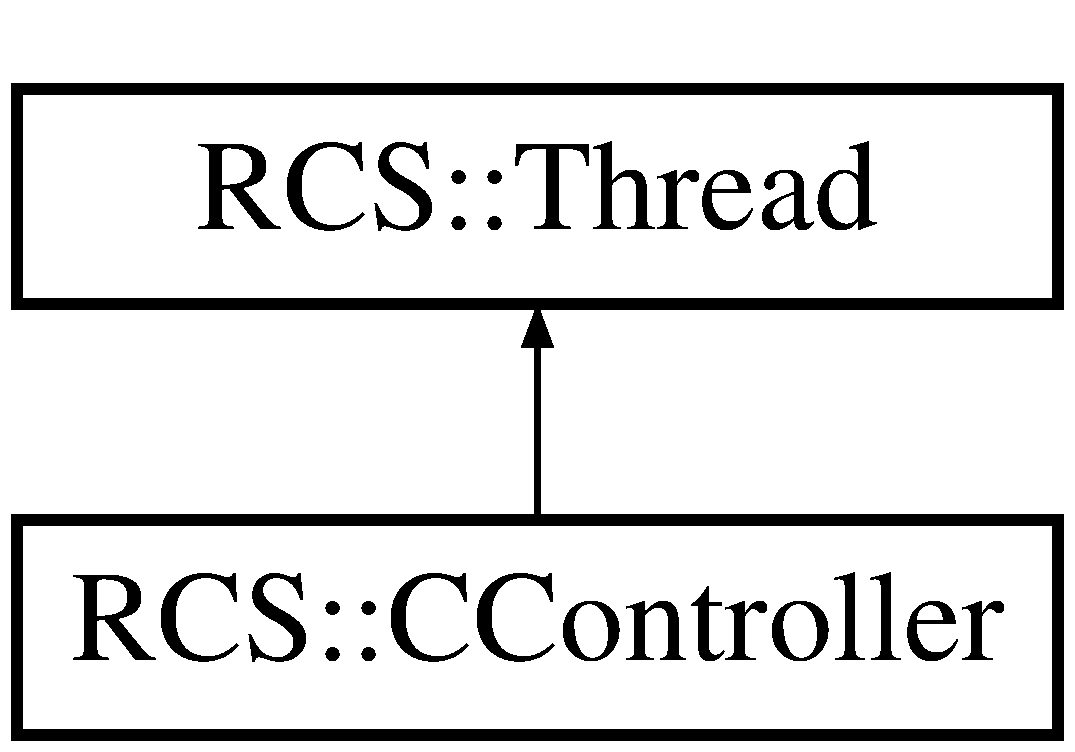
\includegraphics[height=2.000000cm]{structRCS_1_1CController}
\end{center}
\end{figure}
\subsection*{Public Types}
\begin{DoxyCompactItemize}
\item 
enum \hyperlink{structRCS_1_1CController_aeff6d914cf9d714e4c7390de9da446d0}{Debug\-Level} \{ \hyperlink{structRCS_1_1CController_aeff6d914cf9d714e4c7390de9da446d0a30bce5b91d15672b24426d0b2f558225}{F\-A\-T\-A\-L} = 0, 
\hyperlink{structRCS_1_1CController_aeff6d914cf9d714e4c7390de9da446d0a4458583e83012a9eb2309a2d13a1fde9}{W\-A\-R\-N\-I\-N\-G} = 2, 
\hyperlink{structRCS_1_1CController_aeff6d914cf9d714e4c7390de9da446d0adffee45be5e5c4d289cd79e8c64c8365}{I\-N\-F\-O\-R\-M} = 4, 
\hyperlink{structRCS_1_1CController_aeff6d914cf9d714e4c7390de9da446d0af56a0398241628da6412adabec8c3d1f}{F\-U\-L\-L} = 5
 \}
\item 
enum \hyperlink{structRCS_1_1CController_ae1f342838100497b0b94108c6ec74915}{Debug\-Type} \{ \hyperlink{structRCS_1_1CController_ae1f342838100497b0b94108c6ec74915a7028b7cae1fbf32a3ec4c96ea1513242}{C\-R\-C\-L} = 0, 
\hyperlink{structRCS_1_1CController_ae1f342838100497b0b94108c6ec74915aa62b453d8d0e2b7bf2f8a22b9b650441}{R\-P\-Y}
 \}
\item 
enum \hyperlink{structRCS_1_1CController_a50ede7cd9f47204828f0f7c740dc09b1}{Motion\-Planner\-Enum} \{ \\*
\hyperlink{structRCS_1_1CController_a50ede7cd9f47204828f0f7c740dc09b1ab00d7459e4ea68d1b1496592767bfc2f}{N\-O\-P\-L\-A\-N\-N\-E\-R} = 0, 
\hyperlink{structRCS_1_1CController_a50ede7cd9f47204828f0f7c740dc09b1a7904abb74c1bc4246b43b356be0704b5}{M\-O\-V\-E\-I\-T}, 
\hyperlink{structRCS_1_1CController_a50ede7cd9f47204828f0f7c740dc09b1a1506ec08ab80c752e9613c0d42e8accb}{D\-E\-S\-C\-A\-R\-T\-E\-S}, 
\hyperlink{structRCS_1_1CController_a50ede7cd9f47204828f0f7c740dc09b1aa492ff13d221452a2be124f579142e2f}{B\-A\-S\-I\-C}, 
\\*
\hyperlink{structRCS_1_1CController_a50ede7cd9f47204828f0f7c740dc09b1a2a75cf0f1dff3f261dcbf41639f0c2f9}{W\-A\-Y\-P\-O\-I\-N\-T}, 
\hyperlink{structRCS_1_1CController_a50ede7cd9f47204828f0f7c740dc09b1a063b2368ab3f63d194e7b4bc0182410e}{G\-O\-M\-O\-T\-I\-O\-N}
 \}
\item 
typedef std\-::list$<$ \hyperlink{structRCS_1_1CanonCmd}{R\-C\-S\-::\-Canon\-Cmd} $>$ \hyperlink{structRCS_1_1CController_aeaee07d36d39b56ecad1ce2443b5b4c0}{xml\-\_\-message\-\_\-list}
\end{DoxyCompactItemize}
\subsection*{Public Member Functions}
\begin{DoxyCompactItemize}
\item 
\hyperlink{structRCS_1_1CController_acf0744408b45b6d9f60cb44c9d64f1a8}{C\-Controller} (double cycletime)
\begin{DoxyCompactList}\small\item\em \hyperlink{structRCS_1_1CController}{C\-Controller} constructor that requires a cycle time for \hyperlink{namespaceRCS}{R\-C\-S} thread timing. \end{DoxyCompactList}\item 
\hyperlink{structRCS_1_1CController_a2bfe656f4d6a26d3dc4556ed8dab118a}{$\sim$\-C\-Controller} (void)
\item 
bool \hyperlink{structRCS_1_1CController_a7f04bc3e6f36033b2ea18bbac9c34a64}{Verify} ()
\begin{DoxyCompactList}\small\item\em Verifies that all the pointer references in the controller have been instantiated (i.\-e., not null). \end{DoxyCompactList}\item 
virtual int \hyperlink{structRCS_1_1CController_a0ca284e0879e57399044e6700630a526}{Action} ()
\begin{DoxyCompactList}\small\item\em Cyclic loop for the controller. Reads \hyperlink{namespaceCrcl}{Crcl} input mexsage queue, interprets into canon cmds if any, reads canon cmds queue, interprets into robot command messages. \end{DoxyCompactList}\item 
virtual void \hyperlink{structRCS_1_1CController_ad26d222b33f2b043f8a8d8b2b17bac01}{Init} ()
\begin{DoxyCompactList}\small\item\em Initialization routine for the controller.. \end{DoxyCompactList}\item 
std\-::string \hyperlink{structRCS_1_1CController_aa7c4b106c4fb8064d896ccad7ce25b46}{Dump} (std\-::string separator=\char`\"{},\char`\"{})
\begin{DoxyCompactList}\small\item\em Creates a comma separated string of current state of robot. (Can use other separator). \end{DoxyCompactList}\item 
std\-::string \hyperlink{structRCS_1_1CController_aaf2b0286ce10f78e5eee44e3613e588e}{Dump\-Header} (std\-::string separator=\char`\"{},\char`\"{})
\begin{DoxyCompactList}\small\item\em Creates a header line containing names of comma separated string fields that describes the current state of robot. (Can use other separator). \end{DoxyCompactList}\item 
\hyperlink{structRCS_1_1CController_a217e4bc45f9cc45a8b4e927e3e76d9c6}{N\-V\-A\-R} (Crcl\-Delegate, boost\-::shared\-\_\-ptr$<$ \hyperlink{classCrcl_1_1CrclDelegateInterface}{Crcl\-::\-Crcl\-Delegate\-Interface} $>$, crclinterface)
\item 
\hyperlink{structRCS_1_1CController_abb822466798247a45d3206ecae9c36fc}{V\-A\-R} (\hyperlink{SanityCheckTests_8cpp_ac2d60ae645ce73be6021c92b37789e7c}{Kinematics}, boost\-::shared\-\_\-ptr$<$ \hyperlink{classIKinematics}{I\-Kinematics} $>$)
\item 
\hyperlink{structRCS_1_1CController_a220e4784a98f240d3421ae67c79356d2}{V\-A\-R} (Trajectory\-Model, boost\-::shared\-\_\-ptr$<$ \hyperlink{classCTrajectory}{C\-Trajectory} $>$)
\item 
\hyperlink{structRCS_1_1CController_abe34674042d0b1b983a3e4117310f66c}{V\-A\-R} (Joint\-Writer, boost\-::shared\-\_\-ptr$<$ \hyperlink{classCJointWriter}{C\-Joint\-Writer} $>$)
\item 
\hyperlink{structRCS_1_1CController_a4bada8d96b15d19a1b4255f00993a241}{V\-A\-R} (Moveit\-Planner, boost\-::shared\-\_\-ptr$<$ \hyperlink{classMoveitPlanning}{Moveit\-Planning} $>$)
\item 
\hyperlink{structRCS_1_1CController_ad7509a0e8611db8b727493428d1a2a87}{V\-A\-R} (Rviz\-Marker, boost\-::shared\-\_\-ptr$<$ \hyperlink{classCRvizMarker}{C\-Rviz\-Marker} $>$) V\-A\-R(E\-E\-Pose\-Reader
\item 
boost\-::shared\-\_\-ptr$<$ C\-Link\-Reader $>$\\*
 void \hyperlink{structRCS_1_1CController_a2cfc01ab9d46878d06051cf744390542}{Set\-Kinematics} (boost\-::shared\-\_\-ptr$<$ \hyperlink{classIKinematics}{I\-Kinematics} $>$ k)
\begin{DoxyCompactList}\small\item\em Routine to set the kinematics reference pointer. Uses the interface class \hyperlink{classIKinematics}{I\-Kinematics}, but can have any implementation instance. \end{DoxyCompactList}\item 
\hyperlink{structRCS_1_1CController_a5113cb8a1cfaf75459e8a2b13802312e}{N\-V\-A\-R} (New\-C\-C, \hyperlink{structRCS_1_1CanonCmd}{R\-C\-S\-::\-Canon\-Cmd}, \-\_\-newcc)
\item 
\hyperlink{structRCS_1_1CController_a1b85d1d02e33dbfe25173575f17d4498}{N\-V\-A\-R} (Last\-C\-C, \hyperlink{structRCS_1_1CanonCmd}{R\-C\-S\-::\-Canon\-Cmd}, \-\_\-lastcc)
\item 
\hyperlink{structRCS_1_1CanonCmd}{R\-C\-S\-::\-Canon\-Cmd} \hyperlink{structRCS_1_1CController_af150048fb1660e68d9f5ec1043494ea9}{Get\-Last\-Robot\-Command} ()
\item 
\hyperlink{RCS_8h_aa4adb93a26caa4dacba9c9614e283245}{Joint\-State} \hyperlink{structRCS_1_1CController_a7334e3abcc69cc6e3a9f82e59c682551}{Get\-Last\-Joint\-State} ()
\begin{DoxyCompactList}\small\item\em Get the last joint state, if no motion, last actual joint reading, else last joints on robot motion queue. \end{DoxyCompactList}\item 
\hyperlink{namespaceRCS_aa07e45d8a50e30064283d2b38087f999}{R\-C\-S\-::\-Pose} \hyperlink{structRCS_1_1CController_ae7230e4ecd977fb1519b13b2ed696897}{Get\-Last\-Commanded\-Pose} ()
\begin{DoxyCompactList}\small\item\em Get the last commanded , if no motion, use last actual joint reading to compute F\-K, else use last joints on robot motion queue to compute F\-K. \end{DoxyCompactList}\end{DoxyCompactItemize}
\subsection*{Public Attributes}
\begin{DoxyCompactItemize}
\item 
\hyperlink{classRCSInterpreter}{R\-C\-S\-Interpreter} \hyperlink{structRCS_1_1CController_a4c3c287cebfd9fa9fb413205fa0b49f6}{\-\_\-interpreter}
\item 
std\-::string \hyperlink{structRCS_1_1CController_a8bd2705747d1e16f5806ddf183bfade7}{lastlogstatus}
\item 
std\-::string \hyperlink{structRCS_1_1CController_af21d09514563cd2bb2d0d0a5b001d205}{\-\_\-ee\-Name}
\item 
\hyperlink{structRCS_1_1CController_a50ede7cd9f47204828f0f7c740dc09b1}{Motion\-Planner\-Enum} \hyperlink{structRCS_1_1CController_a4174fd5467045e780fe53bde42e70735}{e\-Cartesian\-Motion\-Planner}
\item 
\hyperlink{structRCS_1_1CController_a50ede7cd9f47204828f0f7c740dc09b1}{Motion\-Planner\-Enum} \hyperlink{structRCS_1_1CController_ad788d0def2101be74b680394bcbc78e7}{e\-Joint\-Motion\-Planner}
\end{DoxyCompactItemize}
\subsection*{Static Public Attributes}
\begin{DoxyCompactItemize}
\item 
static bool \hyperlink{structRCS_1_1CController_a5cc727cd1f880d16be6f34d501e06ef0}{b\-Simulation} = true
\item 
static \hyperlink{structRCS_1_1CanonWorldModel}{R\-C\-S\-::\-Canon\-World\-Model} \hyperlink{structRCS_1_1CController_a2b5d355e3e9d6195943ab148c1f94083}{wm}
\item 
static \hyperlink{structRCS_1_1CanonWorldModel}{R\-C\-S\-::\-Canon\-World\-Model} \hyperlink{structRCS_1_1CController_a82e9cc233cd25554964efe8a9008e0b2}{status}
\item 
static \hyperlink{structRCS_1_1CanonWorldModel}{R\-C\-S\-::\-Canon\-World\-Model} \hyperlink{structRCS_1_1CController_af76ac9412dbefbaebc970d62f88a40fa}{laststatus}
\item 
static \hyperlink{classRCS_1_1CMessageQueue}{R\-C\-S\-::\-C\-Message\-Queue}\\*
$<$ \hyperlink{structRCS_1_1CanonCmd}{R\-C\-S\-::\-Canon\-Cmd} $>$ \hyperlink{structRCS_1_1CController_adceba05ebd7fa94f93c131db84840d29}{cmds}
\item 
static \hyperlink{structRCS_1_1CController_aeaee07d36d39b56ecad1ce2443b5b4c0}{xml\-\_\-message\-\_\-list} \hyperlink{structRCS_1_1CController_a093ccebe77526dc736b0ddff70dec0fc}{donecmds}
\item 
static \hyperlink{classRCS_1_1CMessageQueue}{R\-C\-S\-::\-C\-Message\-Queue}\\*
$<$ \hyperlink{structRCS_1_1CanonCmd}{R\-C\-S\-::\-Canon\-Cmd} $>$ \hyperlink{structRCS_1_1CController_aa96c7961737b7e1cf5d8b4180f4bc399}{robotcmds}
\item 
static size\-\_\-t \hyperlink{structRCS_1_1CController_a9b155c29a4fbb8b1a36dada1417126ff}{\-\_\-\-Num\-Joints}
\item 
static bool \hyperlink{structRCS_1_1CController_a5b5e83348fbf18e362a59a2d96668466}{b\-Generate\-Program} = false
\item 
static unsigned long \hyperlink{structRCS_1_1CController_ae4ff5cead0f30ebf8dcbc850b342afc4}{\-\_\-debugtype} = (unsigned long) \hyperlink{structRCS_1_1CController_ae1f342838100497b0b94108c6ec74915aa62b453d8d0e2b7bf2f8a22b9b650441}{R\-P\-Y}
\item 
static unsigned long \hyperlink{structRCS_1_1CController_a1e7f92c361c961fae03b08986bc19a16}{\-\_\-debuglevel} = 0
\item 
static unsigned long \hyperlink{structRCS_1_1CController_ab52a91aa3bfa1f56b527217f09c66912}{\-\_\-csvlog\-Flag} = 0
\item 
static \hyperlink{classALogger}{A\-Logger} \hyperlink{structRCS_1_1CController_a7e21b1156fe37407bae1ba468815206c}{Csv\-Logging}
\end{DoxyCompactItemize}
\subsection*{Additional Inherited Members}


\subsection{Detailed Description}
The \hyperlink{structRCS_1_1CController}{C\-Controller} provides a collection for all the relevant controller pieces. The \hyperlink{structRCS_1_1CController}{C\-Controller} is the main controller class to collect all the references/pointers to instances in the project. A global instance of this class, called \char`\"{}\-Controller\char`\"{}, is created and is used throughout the code to reference various instances of control objects (e.\-g., kinematics, joint writer, joint reader, etc.) 

\subsection{Member Typedef Documentation}
\hypertarget{structRCS_1_1CController_aeaee07d36d39b56ecad1ce2443b5b4c0}{\index{R\-C\-S\-::\-C\-Controller@{R\-C\-S\-::\-C\-Controller}!xml\-\_\-message\-\_\-list@{xml\-\_\-message\-\_\-list}}
\index{xml\-\_\-message\-\_\-list@{xml\-\_\-message\-\_\-list}!RCS::CController@{R\-C\-S\-::\-C\-Controller}}
\subsubsection[{xml\-\_\-message\-\_\-list}]{\setlength{\rightskip}{0pt plus 5cm}typedef std\-::list$<${\bf R\-C\-S\-::\-Canon\-Cmd}$>$ {\bf R\-C\-S\-::\-C\-Controller\-::xml\-\_\-message\-\_\-list}}}\label{structRCS_1_1CController_aeaee07d36d39b56ecad1ce2443b5b4c0}


\subsection{Member Enumeration Documentation}
\hypertarget{structRCS_1_1CController_aeff6d914cf9d714e4c7390de9da446d0}{\index{R\-C\-S\-::\-C\-Controller@{R\-C\-S\-::\-C\-Controller}!Debug\-Level@{Debug\-Level}}
\index{Debug\-Level@{Debug\-Level}!RCS::CController@{R\-C\-S\-::\-C\-Controller}}
\subsubsection[{Debug\-Level}]{\setlength{\rightskip}{0pt plus 5cm}enum {\bf R\-C\-S\-::\-C\-Controller\-::\-Debug\-Level}}}\label{structRCS_1_1CController_aeff6d914cf9d714e4c7390de9da446d0}
\begin{Desc}
\item[Enumerator]\par
\begin{description}
\index{F\-A\-T\-A\-L@{F\-A\-T\-A\-L}!R\-C\-S\-::\-C\-Controller@{R\-C\-S\-::\-C\-Controller}}\index{R\-C\-S\-::\-C\-Controller@{R\-C\-S\-::\-C\-Controller}!F\-A\-T\-A\-L@{F\-A\-T\-A\-L}}\item[{\em 
\hypertarget{structRCS_1_1CController_aeff6d914cf9d714e4c7390de9da446d0a30bce5b91d15672b24426d0b2f558225}{F\-A\-T\-A\-L}\label{structRCS_1_1CController_aeff6d914cf9d714e4c7390de9da446d0a30bce5b91d15672b24426d0b2f558225}
}]\index{W\-A\-R\-N\-I\-N\-G@{W\-A\-R\-N\-I\-N\-G}!R\-C\-S\-::\-C\-Controller@{R\-C\-S\-::\-C\-Controller}}\index{R\-C\-S\-::\-C\-Controller@{R\-C\-S\-::\-C\-Controller}!W\-A\-R\-N\-I\-N\-G@{W\-A\-R\-N\-I\-N\-G}}\item[{\em 
\hypertarget{structRCS_1_1CController_aeff6d914cf9d714e4c7390de9da446d0a4458583e83012a9eb2309a2d13a1fde9}{W\-A\-R\-N\-I\-N\-G}\label{structRCS_1_1CController_aeff6d914cf9d714e4c7390de9da446d0a4458583e83012a9eb2309a2d13a1fde9}
}]\index{I\-N\-F\-O\-R\-M@{I\-N\-F\-O\-R\-M}!R\-C\-S\-::\-C\-Controller@{R\-C\-S\-::\-C\-Controller}}\index{R\-C\-S\-::\-C\-Controller@{R\-C\-S\-::\-C\-Controller}!I\-N\-F\-O\-R\-M@{I\-N\-F\-O\-R\-M}}\item[{\em 
\hypertarget{structRCS_1_1CController_aeff6d914cf9d714e4c7390de9da446d0adffee45be5e5c4d289cd79e8c64c8365}{I\-N\-F\-O\-R\-M}\label{structRCS_1_1CController_aeff6d914cf9d714e4c7390de9da446d0adffee45be5e5c4d289cd79e8c64c8365}
}]\index{F\-U\-L\-L@{F\-U\-L\-L}!R\-C\-S\-::\-C\-Controller@{R\-C\-S\-::\-C\-Controller}}\index{R\-C\-S\-::\-C\-Controller@{R\-C\-S\-::\-C\-Controller}!F\-U\-L\-L@{F\-U\-L\-L}}\item[{\em 
\hypertarget{structRCS_1_1CController_aeff6d914cf9d714e4c7390de9da446d0af56a0398241628da6412adabec8c3d1f}{F\-U\-L\-L}\label{structRCS_1_1CController_aeff6d914cf9d714e4c7390de9da446d0af56a0398241628da6412adabec8c3d1f}
}]\end{description}
\end{Desc}
\hypertarget{structRCS_1_1CController_ae1f342838100497b0b94108c6ec74915}{\index{R\-C\-S\-::\-C\-Controller@{R\-C\-S\-::\-C\-Controller}!Debug\-Type@{Debug\-Type}}
\index{Debug\-Type@{Debug\-Type}!RCS::CController@{R\-C\-S\-::\-C\-Controller}}
\subsubsection[{Debug\-Type}]{\setlength{\rightskip}{0pt plus 5cm}enum {\bf R\-C\-S\-::\-C\-Controller\-::\-Debug\-Type}}}\label{structRCS_1_1CController_ae1f342838100497b0b94108c6ec74915}
\begin{Desc}
\item[Enumerator]\par
\begin{description}
\index{C\-R\-C\-L@{C\-R\-C\-L}!R\-C\-S\-::\-C\-Controller@{R\-C\-S\-::\-C\-Controller}}\index{R\-C\-S\-::\-C\-Controller@{R\-C\-S\-::\-C\-Controller}!C\-R\-C\-L@{C\-R\-C\-L}}\item[{\em 
\hypertarget{structRCS_1_1CController_ae1f342838100497b0b94108c6ec74915a7028b7cae1fbf32a3ec4c96ea1513242}{C\-R\-C\-L}\label{structRCS_1_1CController_ae1f342838100497b0b94108c6ec74915a7028b7cae1fbf32a3ec4c96ea1513242}
}]\index{R\-P\-Y@{R\-P\-Y}!R\-C\-S\-::\-C\-Controller@{R\-C\-S\-::\-C\-Controller}}\index{R\-C\-S\-::\-C\-Controller@{R\-C\-S\-::\-C\-Controller}!R\-P\-Y@{R\-P\-Y}}\item[{\em 
\hypertarget{structRCS_1_1CController_ae1f342838100497b0b94108c6ec74915aa62b453d8d0e2b7bf2f8a22b9b650441}{R\-P\-Y}\label{structRCS_1_1CController_ae1f342838100497b0b94108c6ec74915aa62b453d8d0e2b7bf2f8a22b9b650441}
}]\end{description}
\end{Desc}
\hypertarget{structRCS_1_1CController_a50ede7cd9f47204828f0f7c740dc09b1}{\index{R\-C\-S\-::\-C\-Controller@{R\-C\-S\-::\-C\-Controller}!Motion\-Planner\-Enum@{Motion\-Planner\-Enum}}
\index{Motion\-Planner\-Enum@{Motion\-Planner\-Enum}!RCS::CController@{R\-C\-S\-::\-C\-Controller}}
\subsubsection[{Motion\-Planner\-Enum}]{\setlength{\rightskip}{0pt plus 5cm}enum {\bf R\-C\-S\-::\-C\-Controller\-::\-Motion\-Planner\-Enum}}}\label{structRCS_1_1CController_a50ede7cd9f47204828f0f7c740dc09b1}
\begin{Desc}
\item[Enumerator]\par
\begin{description}
\index{N\-O\-P\-L\-A\-N\-N\-E\-R@{N\-O\-P\-L\-A\-N\-N\-E\-R}!R\-C\-S\-::\-C\-Controller@{R\-C\-S\-::\-C\-Controller}}\index{R\-C\-S\-::\-C\-Controller@{R\-C\-S\-::\-C\-Controller}!N\-O\-P\-L\-A\-N\-N\-E\-R@{N\-O\-P\-L\-A\-N\-N\-E\-R}}\item[{\em 
\hypertarget{structRCS_1_1CController_a50ede7cd9f47204828f0f7c740dc09b1ab00d7459e4ea68d1b1496592767bfc2f}{N\-O\-P\-L\-A\-N\-N\-E\-R}\label{structRCS_1_1CController_a50ede7cd9f47204828f0f7c740dc09b1ab00d7459e4ea68d1b1496592767bfc2f}
}]\index{M\-O\-V\-E\-I\-T@{M\-O\-V\-E\-I\-T}!R\-C\-S\-::\-C\-Controller@{R\-C\-S\-::\-C\-Controller}}\index{R\-C\-S\-::\-C\-Controller@{R\-C\-S\-::\-C\-Controller}!M\-O\-V\-E\-I\-T@{M\-O\-V\-E\-I\-T}}\item[{\em 
\hypertarget{structRCS_1_1CController_a50ede7cd9f47204828f0f7c740dc09b1a7904abb74c1bc4246b43b356be0704b5}{M\-O\-V\-E\-I\-T}\label{structRCS_1_1CController_a50ede7cd9f47204828f0f7c740dc09b1a7904abb74c1bc4246b43b356be0704b5}
}]\index{D\-E\-S\-C\-A\-R\-T\-E\-S@{D\-E\-S\-C\-A\-R\-T\-E\-S}!R\-C\-S\-::\-C\-Controller@{R\-C\-S\-::\-C\-Controller}}\index{R\-C\-S\-::\-C\-Controller@{R\-C\-S\-::\-C\-Controller}!D\-E\-S\-C\-A\-R\-T\-E\-S@{D\-E\-S\-C\-A\-R\-T\-E\-S}}\item[{\em 
\hypertarget{structRCS_1_1CController_a50ede7cd9f47204828f0f7c740dc09b1a1506ec08ab80c752e9613c0d42e8accb}{D\-E\-S\-C\-A\-R\-T\-E\-S}\label{structRCS_1_1CController_a50ede7cd9f47204828f0f7c740dc09b1a1506ec08ab80c752e9613c0d42e8accb}
}]\index{B\-A\-S\-I\-C@{B\-A\-S\-I\-C}!R\-C\-S\-::\-C\-Controller@{R\-C\-S\-::\-C\-Controller}}\index{R\-C\-S\-::\-C\-Controller@{R\-C\-S\-::\-C\-Controller}!B\-A\-S\-I\-C@{B\-A\-S\-I\-C}}\item[{\em 
\hypertarget{structRCS_1_1CController_a50ede7cd9f47204828f0f7c740dc09b1aa492ff13d221452a2be124f579142e2f}{B\-A\-S\-I\-C}\label{structRCS_1_1CController_a50ede7cd9f47204828f0f7c740dc09b1aa492ff13d221452a2be124f579142e2f}
}]\index{W\-A\-Y\-P\-O\-I\-N\-T@{W\-A\-Y\-P\-O\-I\-N\-T}!R\-C\-S\-::\-C\-Controller@{R\-C\-S\-::\-C\-Controller}}\index{R\-C\-S\-::\-C\-Controller@{R\-C\-S\-::\-C\-Controller}!W\-A\-Y\-P\-O\-I\-N\-T@{W\-A\-Y\-P\-O\-I\-N\-T}}\item[{\em 
\hypertarget{structRCS_1_1CController_a50ede7cd9f47204828f0f7c740dc09b1a2a75cf0f1dff3f261dcbf41639f0c2f9}{W\-A\-Y\-P\-O\-I\-N\-T}\label{structRCS_1_1CController_a50ede7cd9f47204828f0f7c740dc09b1a2a75cf0f1dff3f261dcbf41639f0c2f9}
}]\index{G\-O\-M\-O\-T\-I\-O\-N@{G\-O\-M\-O\-T\-I\-O\-N}!R\-C\-S\-::\-C\-Controller@{R\-C\-S\-::\-C\-Controller}}\index{R\-C\-S\-::\-C\-Controller@{R\-C\-S\-::\-C\-Controller}!G\-O\-M\-O\-T\-I\-O\-N@{G\-O\-M\-O\-T\-I\-O\-N}}\item[{\em 
\hypertarget{structRCS_1_1CController_a50ede7cd9f47204828f0f7c740dc09b1a063b2368ab3f63d194e7b4bc0182410e}{G\-O\-M\-O\-T\-I\-O\-N}\label{structRCS_1_1CController_a50ede7cd9f47204828f0f7c740dc09b1a063b2368ab3f63d194e7b4bc0182410e}
}]\end{description}
\end{Desc}


\subsection{Constructor \& Destructor Documentation}
\hypertarget{structRCS_1_1CController_acf0744408b45b6d9f60cb44c9d64f1a8}{\index{R\-C\-S\-::\-C\-Controller@{R\-C\-S\-::\-C\-Controller}!C\-Controller@{C\-Controller}}
\index{C\-Controller@{C\-Controller}!RCS::CController@{R\-C\-S\-::\-C\-Controller}}
\subsubsection[{C\-Controller}]{\setlength{\rightskip}{0pt plus 5cm}R\-C\-S\-::\-C\-Controller\-::\-C\-Controller (
\begin{DoxyParamCaption}
\item[{double}]{cycletime}
\end{DoxyParamCaption}
)}}\label{structRCS_1_1CController_acf0744408b45b6d9f60cb44c9d64f1a8}


\hyperlink{structRCS_1_1CController}{C\-Controller} constructor that requires a cycle time for \hyperlink{namespaceRCS}{R\-C\-S} thread timing. 


\begin{DoxyParams}{Parameters}
{\em cycletime} & in seconds. \\
\hline
\end{DoxyParams}
\hypertarget{structRCS_1_1CController_a2bfe656f4d6a26d3dc4556ed8dab118a}{\index{R\-C\-S\-::\-C\-Controller@{R\-C\-S\-::\-C\-Controller}!$\sim$\-C\-Controller@{$\sim$\-C\-Controller}}
\index{$\sim$\-C\-Controller@{$\sim$\-C\-Controller}!RCS::CController@{R\-C\-S\-::\-C\-Controller}}
\subsubsection[{$\sim$\-C\-Controller}]{\setlength{\rightskip}{0pt plus 5cm}R\-C\-S\-::\-C\-Controller\-::$\sim$\-C\-Controller (
\begin{DoxyParamCaption}
\item[{void}]{}
\end{DoxyParamCaption}
)}}\label{structRCS_1_1CController_a2bfe656f4d6a26d3dc4556ed8dab118a}


\subsection{Member Function Documentation}
\hypertarget{structRCS_1_1CController_a0ca284e0879e57399044e6700630a526}{\index{R\-C\-S\-::\-C\-Controller@{R\-C\-S\-::\-C\-Controller}!Action@{Action}}
\index{Action@{Action}!RCS::CController@{R\-C\-S\-::\-C\-Controller}}
\subsubsection[{Action}]{\setlength{\rightskip}{0pt plus 5cm}int R\-C\-S\-::\-C\-Controller\-::\-Action (
\begin{DoxyParamCaption}
{}
\end{DoxyParamCaption}
)\hspace{0.3cm}{\ttfamily [virtual]}}}\label{structRCS_1_1CController_a0ca284e0879e57399044e6700630a526}


Cyclic loop for the controller. Reads \hyperlink{namespaceCrcl}{Crcl} input mexsage queue, interprets into canon cmds if any, reads canon cmds queue, interprets into robot command messages. 



Reimplemented from \hyperlink{classRCS_1_1Thread_a78aec7128f4fbf5d6859ceb09f9f9ae1}{R\-C\-S\-::\-Thread}.

\hypertarget{structRCS_1_1CController_aa7c4b106c4fb8064d896ccad7ce25b46}{\index{R\-C\-S\-::\-C\-Controller@{R\-C\-S\-::\-C\-Controller}!Dump@{Dump}}
\index{Dump@{Dump}!RCS::CController@{R\-C\-S\-::\-C\-Controller}}
\subsubsection[{Dump}]{\setlength{\rightskip}{0pt plus 5cm}std\-::string R\-C\-S\-::\-C\-Controller\-::\-Dump (
\begin{DoxyParamCaption}
\item[{std\-::string}]{separator = {\ttfamily \char`\"{},\char`\"{}}}
\end{DoxyParamCaption}
)}}\label{structRCS_1_1CController_aa7c4b106c4fb8064d896ccad7ce25b46}


Creates a comma separated string of current state of robot. (Can use other separator). 

\hypertarget{structRCS_1_1CController_aaf2b0286ce10f78e5eee44e3613e588e}{\index{R\-C\-S\-::\-C\-Controller@{R\-C\-S\-::\-C\-Controller}!Dump\-Header@{Dump\-Header}}
\index{Dump\-Header@{Dump\-Header}!RCS::CController@{R\-C\-S\-::\-C\-Controller}}
\subsubsection[{Dump\-Header}]{\setlength{\rightskip}{0pt plus 5cm}std\-::string R\-C\-S\-::\-C\-Controller\-::\-Dump\-Header (
\begin{DoxyParamCaption}
\item[{std\-::string}]{separator = {\ttfamily \char`\"{},\char`\"{}}}
\end{DoxyParamCaption}
)}}\label{structRCS_1_1CController_aaf2b0286ce10f78e5eee44e3613e588e}


Creates a header line containing names of comma separated string fields that describes the current state of robot. (Can use other separator). 

\hypertarget{structRCS_1_1CController_ae7230e4ecd977fb1519b13b2ed696897}{\index{R\-C\-S\-::\-C\-Controller@{R\-C\-S\-::\-C\-Controller}!Get\-Last\-Commanded\-Pose@{Get\-Last\-Commanded\-Pose}}
\index{Get\-Last\-Commanded\-Pose@{Get\-Last\-Commanded\-Pose}!RCS::CController@{R\-C\-S\-::\-C\-Controller}}
\subsubsection[{Get\-Last\-Commanded\-Pose}]{\setlength{\rightskip}{0pt plus 5cm}{\bf R\-C\-S\-::\-Pose} R\-C\-S\-::\-C\-Controller\-::\-Get\-Last\-Commanded\-Pose (
\begin{DoxyParamCaption}
{}
\end{DoxyParamCaption}
)}}\label{structRCS_1_1CController_ae7230e4ecd977fb1519b13b2ed696897}


Get the last commanded , if no motion, use last actual joint reading to compute F\-K, else use last joints on robot motion queue to compute F\-K. 

\hypertarget{structRCS_1_1CController_a7334e3abcc69cc6e3a9f82e59c682551}{\index{R\-C\-S\-::\-C\-Controller@{R\-C\-S\-::\-C\-Controller}!Get\-Last\-Joint\-State@{Get\-Last\-Joint\-State}}
\index{Get\-Last\-Joint\-State@{Get\-Last\-Joint\-State}!RCS::CController@{R\-C\-S\-::\-C\-Controller}}
\subsubsection[{Get\-Last\-Joint\-State}]{\setlength{\rightskip}{0pt plus 5cm}{\bf Joint\-State} R\-C\-S\-::\-C\-Controller\-::\-Get\-Last\-Joint\-State (
\begin{DoxyParamCaption}
{}
\end{DoxyParamCaption}
)}}\label{structRCS_1_1CController_a7334e3abcc69cc6e3a9f82e59c682551}


Get the last joint state, if no motion, last actual joint reading, else last joints on robot motion queue. 

\hypertarget{structRCS_1_1CController_af150048fb1660e68d9f5ec1043494ea9}{\index{R\-C\-S\-::\-C\-Controller@{R\-C\-S\-::\-C\-Controller}!Get\-Last\-Robot\-Command@{Get\-Last\-Robot\-Command}}
\index{Get\-Last\-Robot\-Command@{Get\-Last\-Robot\-Command}!RCS::CController@{R\-C\-S\-::\-C\-Controller}}
\subsubsection[{Get\-Last\-Robot\-Command}]{\setlength{\rightskip}{0pt plus 5cm}{\bf R\-C\-S\-::\-Canon\-Cmd} R\-C\-S\-::\-C\-Controller\-::\-Get\-Last\-Robot\-Command (
\begin{DoxyParamCaption}
{}
\end{DoxyParamCaption}
)}}\label{structRCS_1_1CController_af150048fb1660e68d9f5ec1043494ea9}
\hypertarget{structRCS_1_1CController_ad26d222b33f2b043f8a8d8b2b17bac01}{\index{R\-C\-S\-::\-C\-Controller@{R\-C\-S\-::\-C\-Controller}!Init@{Init}}
\index{Init@{Init}!RCS::CController@{R\-C\-S\-::\-C\-Controller}}
\subsubsection[{Init}]{\setlength{\rightskip}{0pt plus 5cm}void R\-C\-S\-::\-C\-Controller\-::\-Init (
\begin{DoxyParamCaption}
{}
\end{DoxyParamCaption}
)\hspace{0.3cm}{\ttfamily [virtual]}}}\label{structRCS_1_1CController_ad26d222b33f2b043f8a8d8b2b17bac01}


Initialization routine for the controller.. 



Reimplemented from \hyperlink{classRCS_1_1Thread_a53ee19c04d064c9a23f0909cf9a4b2cc}{R\-C\-S\-::\-Thread}.

\hypertarget{structRCS_1_1CController_a217e4bc45f9cc45a8b4e927e3e76d9c6}{\index{R\-C\-S\-::\-C\-Controller@{R\-C\-S\-::\-C\-Controller}!N\-V\-A\-R@{N\-V\-A\-R}}
\index{N\-V\-A\-R@{N\-V\-A\-R}!RCS::CController@{R\-C\-S\-::\-C\-Controller}}
\subsubsection[{N\-V\-A\-R}]{\setlength{\rightskip}{0pt plus 5cm}R\-C\-S\-::\-C\-Controller\-::\-N\-V\-A\-R (
\begin{DoxyParamCaption}
\item[{Crcl\-Delegate}]{, }
\item[{boost\-::shared\-\_\-ptr$<$ {\bf Crcl\-::\-Crcl\-Delegate\-Interface} $>$}]{, }
\item[{crclinterface}]{}
\end{DoxyParamCaption}
)}}\label{structRCS_1_1CController_a217e4bc45f9cc45a8b4e927e3e76d9c6}
\hypertarget{structRCS_1_1CController_a5113cb8a1cfaf75459e8a2b13802312e}{\index{R\-C\-S\-::\-C\-Controller@{R\-C\-S\-::\-C\-Controller}!N\-V\-A\-R@{N\-V\-A\-R}}
\index{N\-V\-A\-R@{N\-V\-A\-R}!RCS::CController@{R\-C\-S\-::\-C\-Controller}}
\subsubsection[{N\-V\-A\-R}]{\setlength{\rightskip}{0pt plus 5cm}R\-C\-S\-::\-C\-Controller\-::\-N\-V\-A\-R (
\begin{DoxyParamCaption}
\item[{New\-C\-C}]{, }
\item[{{\bf R\-C\-S\-::\-Canon\-Cmd}}]{, }
\item[{\-\_\-newcc}]{}
\end{DoxyParamCaption}
)}}\label{structRCS_1_1CController_a5113cb8a1cfaf75459e8a2b13802312e}
last canon command interpreted \hypertarget{structRCS_1_1CController_a1b85d1d02e33dbfe25173575f17d4498}{\index{R\-C\-S\-::\-C\-Controller@{R\-C\-S\-::\-C\-Controller}!N\-V\-A\-R@{N\-V\-A\-R}}
\index{N\-V\-A\-R@{N\-V\-A\-R}!RCS::CController@{R\-C\-S\-::\-C\-Controller}}
\subsubsection[{N\-V\-A\-R}]{\setlength{\rightskip}{0pt plus 5cm}R\-C\-S\-::\-C\-Controller\-::\-N\-V\-A\-R (
\begin{DoxyParamCaption}
\item[{Last\-C\-C}]{, }
\item[{{\bf R\-C\-S\-::\-Canon\-Cmd}}]{, }
\item[{\-\_\-lastcc}]{}
\end{DoxyParamCaption}
)}}\label{structRCS_1_1CController_a1b85d1d02e33dbfe25173575f17d4498}
\hypertarget{structRCS_1_1CController_a2cfc01ab9d46878d06051cf744390542}{\index{R\-C\-S\-::\-C\-Controller@{R\-C\-S\-::\-C\-Controller}!Set\-Kinematics@{Set\-Kinematics}}
\index{Set\-Kinematics@{Set\-Kinematics}!RCS::CController@{R\-C\-S\-::\-C\-Controller}}
\subsubsection[{Set\-Kinematics}]{\setlength{\rightskip}{0pt plus 5cm}boost\-::shared\-\_\-ptr$<$C\-Link\-Reader$>$ void R\-C\-S\-::\-C\-Controller\-::\-Set\-Kinematics (
\begin{DoxyParamCaption}
\item[{boost\-::shared\-\_\-ptr$<$ {\bf I\-Kinematics} $>$}]{k}
\end{DoxyParamCaption}
)\hspace{0.3cm}{\ttfamily [inline]}}}\label{structRCS_1_1CController_a2cfc01ab9d46878d06051cf744390542}


Routine to set the kinematics reference pointer. Uses the interface class \hyperlink{classIKinematics}{I\-Kinematics}, but can have any implementation instance. 

\hypertarget{structRCS_1_1CController_abb822466798247a45d3206ecae9c36fc}{\index{R\-C\-S\-::\-C\-Controller@{R\-C\-S\-::\-C\-Controller}!V\-A\-R@{V\-A\-R}}
\index{V\-A\-R@{V\-A\-R}!RCS::CController@{R\-C\-S\-::\-C\-Controller}}
\subsubsection[{V\-A\-R}]{\setlength{\rightskip}{0pt plus 5cm}R\-C\-S\-::\-C\-Controller\-::\-V\-A\-R (
\begin{DoxyParamCaption}
\item[{{\bf Kinematics}}]{, }
\item[{boost\-::shared\-\_\-ptr$<$ {\bf I\-Kinematics} $>$}]{}
\end{DoxyParamCaption}
)}}\label{structRCS_1_1CController_abb822466798247a45d3206ecae9c36fc}
\hypertarget{structRCS_1_1CController_a220e4784a98f240d3421ae67c79356d2}{\index{R\-C\-S\-::\-C\-Controller@{R\-C\-S\-::\-C\-Controller}!V\-A\-R@{V\-A\-R}}
\index{V\-A\-R@{V\-A\-R}!RCS::CController@{R\-C\-S\-::\-C\-Controller}}
\subsubsection[{V\-A\-R}]{\setlength{\rightskip}{0pt plus 5cm}R\-C\-S\-::\-C\-Controller\-::\-V\-A\-R (
\begin{DoxyParamCaption}
\item[{Trajectory\-Model}]{, }
\item[{boost\-::shared\-\_\-ptr$<$ {\bf C\-Trajectory} $>$}]{}
\end{DoxyParamCaption}
)}}\label{structRCS_1_1CController_a220e4784a98f240d3421ae67c79356d2}
\hypertarget{structRCS_1_1CController_abe34674042d0b1b983a3e4117310f66c}{\index{R\-C\-S\-::\-C\-Controller@{R\-C\-S\-::\-C\-Controller}!V\-A\-R@{V\-A\-R}}
\index{V\-A\-R@{V\-A\-R}!RCS::CController@{R\-C\-S\-::\-C\-Controller}}
\subsubsection[{V\-A\-R}]{\setlength{\rightskip}{0pt plus 5cm}R\-C\-S\-::\-C\-Controller\-::\-V\-A\-R (
\begin{DoxyParamCaption}
\item[{Joint\-Writer}]{, }
\item[{boost\-::shared\-\_\-ptr$<$ {\bf C\-Joint\-Writer} $>$}]{}
\end{DoxyParamCaption}
)}}\label{structRCS_1_1CController_abe34674042d0b1b983a3e4117310f66c}
\hypertarget{structRCS_1_1CController_a4bada8d96b15d19a1b4255f00993a241}{\index{R\-C\-S\-::\-C\-Controller@{R\-C\-S\-::\-C\-Controller}!V\-A\-R@{V\-A\-R}}
\index{V\-A\-R@{V\-A\-R}!RCS::CController@{R\-C\-S\-::\-C\-Controller}}
\subsubsection[{V\-A\-R}]{\setlength{\rightskip}{0pt plus 5cm}R\-C\-S\-::\-C\-Controller\-::\-V\-A\-R (
\begin{DoxyParamCaption}
\item[{Moveit\-Planner}]{, }
\item[{boost\-::shared\-\_\-ptr$<$ {\bf Moveit\-Planning} $>$}]{}
\end{DoxyParamCaption}
)}}\label{structRCS_1_1CController_a4bada8d96b15d19a1b4255f00993a241}
\hypertarget{structRCS_1_1CController_ad7509a0e8611db8b727493428d1a2a87}{\index{R\-C\-S\-::\-C\-Controller@{R\-C\-S\-::\-C\-Controller}!V\-A\-R@{V\-A\-R}}
\index{V\-A\-R@{V\-A\-R}!RCS::CController@{R\-C\-S\-::\-C\-Controller}}
\subsubsection[{V\-A\-R}]{\setlength{\rightskip}{0pt plus 5cm}R\-C\-S\-::\-C\-Controller\-::\-V\-A\-R (
\begin{DoxyParamCaption}
\item[{Rviz\-Marker}]{, }
\item[{boost\-::shared\-\_\-ptr$<$ {\bf C\-Rviz\-Marker} $>$}]{}
\end{DoxyParamCaption}
)}}\label{structRCS_1_1CController_ad7509a0e8611db8b727493428d1a2a87}
\hypertarget{structRCS_1_1CController_a7f04bc3e6f36033b2ea18bbac9c34a64}{\index{R\-C\-S\-::\-C\-Controller@{R\-C\-S\-::\-C\-Controller}!Verify@{Verify}}
\index{Verify@{Verify}!RCS::CController@{R\-C\-S\-::\-C\-Controller}}
\subsubsection[{Verify}]{\setlength{\rightskip}{0pt plus 5cm}bool R\-C\-S\-::\-C\-Controller\-::\-Verify (
\begin{DoxyParamCaption}
{}
\end{DoxyParamCaption}
)}}\label{structRCS_1_1CController_a7f04bc3e6f36033b2ea18bbac9c34a64}


Verifies that all the pointer references in the controller have been instantiated (i.\-e., not null). 



\subsection{Member Data Documentation}
\hypertarget{structRCS_1_1CController_ab52a91aa3bfa1f56b527217f09c66912}{\index{R\-C\-S\-::\-C\-Controller@{R\-C\-S\-::\-C\-Controller}!\-\_\-csvlog\-Flag@{\-\_\-csvlog\-Flag}}
\index{\-\_\-csvlog\-Flag@{\-\_\-csvlog\-Flag}!RCS::CController@{R\-C\-S\-::\-C\-Controller}}
\subsubsection[{\-\_\-csvlog\-Flag}]{\setlength{\rightskip}{0pt plus 5cm}unsigned long R\-C\-S\-::\-C\-Controller\-::\-\_\-csvlog\-Flag = 0\hspace{0.3cm}{\ttfamily [static]}}}\label{structRCS_1_1CController_ab52a91aa3bfa1f56b527217f09c66912}
\hypertarget{structRCS_1_1CController_a1e7f92c361c961fae03b08986bc19a16}{\index{R\-C\-S\-::\-C\-Controller@{R\-C\-S\-::\-C\-Controller}!\-\_\-debuglevel@{\-\_\-debuglevel}}
\index{\-\_\-debuglevel@{\-\_\-debuglevel}!RCS::CController@{R\-C\-S\-::\-C\-Controller}}
\subsubsection[{\-\_\-debuglevel}]{\setlength{\rightskip}{0pt plus 5cm}unsigned long R\-C\-S\-::\-C\-Controller\-::\-\_\-debuglevel = 0\hspace{0.3cm}{\ttfamily [static]}}}\label{structRCS_1_1CController_a1e7f92c361c961fae03b08986bc19a16}
level of debugging, 0 least, 5 most \hypertarget{structRCS_1_1CController_ae4ff5cead0f30ebf8dcbc850b342afc4}{\index{R\-C\-S\-::\-C\-Controller@{R\-C\-S\-::\-C\-Controller}!\-\_\-debugtype@{\-\_\-debugtype}}
\index{\-\_\-debugtype@{\-\_\-debugtype}!RCS::CController@{R\-C\-S\-::\-C\-Controller}}
\subsubsection[{\-\_\-debugtype}]{\setlength{\rightskip}{0pt plus 5cm}unsigned long R\-C\-S\-::\-C\-Controller\-::\-\_\-debugtype = (unsigned long) {\bf R\-P\-Y}\hspace{0.3cm}{\ttfamily [static]}}}\label{structRCS_1_1CController_ae4ff5cead0f30ebf8dcbc850b342afc4}
output crcl xz rotation or roll,pitch, yaw \hypertarget{structRCS_1_1CController_af21d09514563cd2bb2d0d0a5b001d205}{\index{R\-C\-S\-::\-C\-Controller@{R\-C\-S\-::\-C\-Controller}!\-\_\-ee\-Name@{\-\_\-ee\-Name}}
\index{\-\_\-ee\-Name@{\-\_\-ee\-Name}!RCS::CController@{R\-C\-S\-::\-C\-Controller}}
\subsubsection[{\-\_\-ee\-Name}]{\setlength{\rightskip}{0pt plus 5cm}std\-::string R\-C\-S\-::\-C\-Controller\-::\-\_\-ee\-Name}}\label{structRCS_1_1CController_af21d09514563cd2bb2d0d0a5b001d205}
\hypertarget{structRCS_1_1CController_a4c3c287cebfd9fa9fb413205fa0b49f6}{\index{R\-C\-S\-::\-C\-Controller@{R\-C\-S\-::\-C\-Controller}!\-\_\-interpreter@{\-\_\-interpreter}}
\index{\-\_\-interpreter@{\-\_\-interpreter}!RCS::CController@{R\-C\-S\-::\-C\-Controller}}
\subsubsection[{\-\_\-interpreter}]{\setlength{\rightskip}{0pt plus 5cm}{\bf R\-C\-S\-Interpreter} R\-C\-S\-::\-C\-Controller\-::\-\_\-interpreter}}\label{structRCS_1_1CController_a4c3c287cebfd9fa9fb413205fa0b49f6}
interprets canon commands into robot commands current new canon command to interpret \hypertarget{structRCS_1_1CController_a9b155c29a4fbb8b1a36dada1417126ff}{\index{R\-C\-S\-::\-C\-Controller@{R\-C\-S\-::\-C\-Controller}!\-\_\-\-Num\-Joints@{\-\_\-\-Num\-Joints}}
\index{\-\_\-\-Num\-Joints@{\-\_\-\-Num\-Joints}!RCS::CController@{R\-C\-S\-::\-C\-Controller}}
\subsubsection[{\-\_\-\-Num\-Joints}]{\setlength{\rightskip}{0pt plus 5cm}size\-\_\-t R\-C\-S\-::\-C\-Controller\-::\-\_\-\-Num\-Joints\hspace{0.3cm}{\ttfamily [static]}}}\label{structRCS_1_1CController_a9b155c29a4fbb8b1a36dada1417126ff}
number of joints in controller robot -\/ assuming serial link manipulator \hypertarget{structRCS_1_1CController_a5b5e83348fbf18e362a59a2d96668466}{\index{R\-C\-S\-::\-C\-Controller@{R\-C\-S\-::\-C\-Controller}!b\-Generate\-Program@{b\-Generate\-Program}}
\index{b\-Generate\-Program@{b\-Generate\-Program}!RCS::CController@{R\-C\-S\-::\-C\-Controller}}
\subsubsection[{b\-Generate\-Program}]{\setlength{\rightskip}{0pt plus 5cm}bool R\-C\-S\-::\-C\-Controller\-::b\-Generate\-Program = false\hspace{0.3cm}{\ttfamily [static]}}}\label{structRCS_1_1CController_a5b5e83348fbf18e362a59a2d96668466}
global flag to create program from \hyperlink{namespaceCrcl}{Crcl} X\-M\-L \hypertarget{structRCS_1_1CController_a5cc727cd1f880d16be6f34d501e06ef0}{\index{R\-C\-S\-::\-C\-Controller@{R\-C\-S\-::\-C\-Controller}!b\-Simulation@{b\-Simulation}}
\index{b\-Simulation@{b\-Simulation}!RCS::CController@{R\-C\-S\-::\-C\-Controller}}
\subsubsection[{b\-Simulation}]{\setlength{\rightskip}{0pt plus 5cm}bool R\-C\-S\-::\-C\-Controller\-::b\-Simulation = true\hspace{0.3cm}{\ttfamily [static]}}}\label{structRCS_1_1CController_a5cc727cd1f880d16be6f34d501e06ef0}
simulation flag -\/ not connected to robot \hypertarget{structRCS_1_1CController_adceba05ebd7fa94f93c131db84840d29}{\index{R\-C\-S\-::\-C\-Controller@{R\-C\-S\-::\-C\-Controller}!cmds@{cmds}}
\index{cmds@{cmds}!RCS::CController@{R\-C\-S\-::\-C\-Controller}}
\subsubsection[{cmds}]{\setlength{\rightskip}{0pt plus 5cm}{\bf R\-C\-S\-::\-C\-Message\-Queue}$<$ {\bf R\-C\-S\-::\-Canon\-Cmd} $>$ R\-C\-S\-::\-C\-Controller\-::cmds\hspace{0.3cm}{\ttfamily [static]}}}\label{structRCS_1_1CController_adceba05ebd7fa94f93c131db84840d29}
queue of commands interpreted from \hyperlink{namespaceCrcl}{Crcl} messages \hypertarget{structRCS_1_1CController_a7e21b1156fe37407bae1ba468815206c}{\index{R\-C\-S\-::\-C\-Controller@{R\-C\-S\-::\-C\-Controller}!Csv\-Logging@{Csv\-Logging}}
\index{Csv\-Logging@{Csv\-Logging}!RCS::CController@{R\-C\-S\-::\-C\-Controller}}
\subsubsection[{Csv\-Logging}]{\setlength{\rightskip}{0pt plus 5cm}{\bf A\-Logger} R\-C\-S\-::\-C\-Controller\-::\-Csv\-Logging\hspace{0.3cm}{\ttfamily [static]}}}\label{structRCS_1_1CController_a7e21b1156fe37407bae1ba468815206c}
controller status csv logging instance \hypertarget{structRCS_1_1CController_a093ccebe77526dc736b0ddff70dec0fc}{\index{R\-C\-S\-::\-C\-Controller@{R\-C\-S\-::\-C\-Controller}!donecmds@{donecmds}}
\index{donecmds@{donecmds}!RCS::CController@{R\-C\-S\-::\-C\-Controller}}
\subsubsection[{donecmds}]{\setlength{\rightskip}{0pt plus 5cm}{\bf R\-C\-S\-::\-C\-Controller\-::xml\-\_\-message\-\_\-list} R\-C\-S\-::\-C\-Controller\-::donecmds\hspace{0.3cm}{\ttfamily [static]}}}\label{structRCS_1_1CController_a093ccebe77526dc736b0ddff70dec0fc}
list of commands interpreted from \hyperlink{namespaceCrcl}{Crcl} messages that have completed \hypertarget{structRCS_1_1CController_a4174fd5467045e780fe53bde42e70735}{\index{R\-C\-S\-::\-C\-Controller@{R\-C\-S\-::\-C\-Controller}!e\-Cartesian\-Motion\-Planner@{e\-Cartesian\-Motion\-Planner}}
\index{e\-Cartesian\-Motion\-Planner@{e\-Cartesian\-Motion\-Planner}!RCS::CController@{R\-C\-S\-::\-C\-Controller}}
\subsubsection[{e\-Cartesian\-Motion\-Planner}]{\setlength{\rightskip}{0pt plus 5cm}{\bf Motion\-Planner\-Enum} R\-C\-S\-::\-C\-Controller\-::e\-Cartesian\-Motion\-Planner}}\label{structRCS_1_1CController_a4174fd5467045e780fe53bde42e70735}
type of cartesian motion to use \hypertarget{structRCS_1_1CController_ad788d0def2101be74b680394bcbc78e7}{\index{R\-C\-S\-::\-C\-Controller@{R\-C\-S\-::\-C\-Controller}!e\-Joint\-Motion\-Planner@{e\-Joint\-Motion\-Planner}}
\index{e\-Joint\-Motion\-Planner@{e\-Joint\-Motion\-Planner}!RCS::CController@{R\-C\-S\-::\-C\-Controller}}
\subsubsection[{e\-Joint\-Motion\-Planner}]{\setlength{\rightskip}{0pt plus 5cm}{\bf Motion\-Planner\-Enum} R\-C\-S\-::\-C\-Controller\-::e\-Joint\-Motion\-Planner}}\label{structRCS_1_1CController_ad788d0def2101be74b680394bcbc78e7}
type of joint motion to use \hypertarget{structRCS_1_1CController_a8bd2705747d1e16f5806ddf183bfade7}{\index{R\-C\-S\-::\-C\-Controller@{R\-C\-S\-::\-C\-Controller}!lastlogstatus@{lastlogstatus}}
\index{lastlogstatus@{lastlogstatus}!RCS::CController@{R\-C\-S\-::\-C\-Controller}}
\subsubsection[{lastlogstatus}]{\setlength{\rightskip}{0pt plus 5cm}std\-::string R\-C\-S\-::\-C\-Controller\-::lastlogstatus}}\label{structRCS_1_1CController_a8bd2705747d1e16f5806ddf183bfade7}
\hypertarget{structRCS_1_1CController_af76ac9412dbefbaebc970d62f88a40fa}{\index{R\-C\-S\-::\-C\-Controller@{R\-C\-S\-::\-C\-Controller}!laststatus@{laststatus}}
\index{laststatus@{laststatus}!RCS::CController@{R\-C\-S\-::\-C\-Controller}}
\subsubsection[{laststatus}]{\setlength{\rightskip}{0pt plus 5cm}{\bf R\-C\-S\-::\-Canon\-World\-Model} R\-C\-S\-::\-C\-Controller\-::laststatus\hspace{0.3cm}{\ttfamily [static]}}}\label{structRCS_1_1CController_af76ac9412dbefbaebc970d62f88a40fa}
last status of controller \hypertarget{structRCS_1_1CController_aa96c7961737b7e1cf5d8b4180f4bc399}{\index{R\-C\-S\-::\-C\-Controller@{R\-C\-S\-::\-C\-Controller}!robotcmds@{robotcmds}}
\index{robotcmds@{robotcmds}!RCS::CController@{R\-C\-S\-::\-C\-Controller}}
\subsubsection[{robotcmds}]{\setlength{\rightskip}{0pt plus 5cm}{\bf R\-C\-S\-::\-C\-Message\-Queue}$<$ {\bf R\-C\-S\-::\-Canon\-Cmd} $>$ R\-C\-S\-::\-C\-Controller\-::robotcmds\hspace{0.3cm}{\ttfamily [static]}}}\label{structRCS_1_1CController_aa96c7961737b7e1cf5d8b4180f4bc399}
list of commands to be sent to robot \hypertarget{structRCS_1_1CController_a82e9cc233cd25554964efe8a9008e0b2}{\index{R\-C\-S\-::\-C\-Controller@{R\-C\-S\-::\-C\-Controller}!status@{status}}
\index{status@{status}!RCS::CController@{R\-C\-S\-::\-C\-Controller}}
\subsubsection[{status}]{\setlength{\rightskip}{0pt plus 5cm}{\bf R\-C\-S\-::\-Canon\-World\-Model} R\-C\-S\-::\-C\-Controller\-::status\hspace{0.3cm}{\ttfamily [static]}}}\label{structRCS_1_1CController_a82e9cc233cd25554964efe8a9008e0b2}
current status of controller \hypertarget{structRCS_1_1CController_a2b5d355e3e9d6195943ab148c1f94083}{\index{R\-C\-S\-::\-C\-Controller@{R\-C\-S\-::\-C\-Controller}!wm@{wm}}
\index{wm@{wm}!RCS::CController@{R\-C\-S\-::\-C\-Controller}}
\subsubsection[{wm}]{\setlength{\rightskip}{0pt plus 5cm}{\bf R\-C\-S\-::\-Canon\-World\-Model} R\-C\-S\-::\-C\-Controller\-::wm\hspace{0.3cm}{\ttfamily [static]}}}\label{structRCS_1_1CController_a2b5d355e3e9d6195943ab148c1f94083}
the world model of the controller 

The documentation for this struct was generated from the following files\-:\begin{DoxyCompactItemize}
\item 
/usr/local/michalos/github/usnistgov/el-\/robotics-\/core/nist\-\_\-fanuc/include/nist\-\_\-fanuc/\hyperlink{Controller_8h}{Controller.\-h}\item 
/usr/local/michalos/github/usnistgov/el-\/robotics-\/core/nist\-\_\-fanuc/src/\hyperlink{Controller_8cpp}{Controller.\-cpp}\end{DoxyCompactItemize}

\hypertarget{classCGlobals}{\section{C\-Globals Class Reference}
\label{classCGlobals}\index{C\-Globals@{C\-Globals}}
}


\hyperlink{classCGlobals}{C\-Globals} is a catch-\/all data structure for collecting global functions, extensions, parameters, etc. Functions here usually vary between windows and linux, or there is no easy mechanism in C++ to extend classes (e.\-g., string) like in C\#.  




{\ttfamily \#include $<$Globals.\-h$>$}

\subsection*{Public Types}
\begin{DoxyCompactItemize}
\item 
enum \hyperlink{classCGlobals_a32f8f289bca445b5a2f6d1c68b6cbbb2}{Time\-Format} \{ \hyperlink{classCGlobals_a32f8f289bca445b5a2f6d1c68b6cbbb2a98adc6b59af1736f60ba1f8463521dc1}{H\-U\-M\-\_\-\-R\-E\-A\-D}, 
\hyperlink{classCGlobals_a32f8f289bca445b5a2f6d1c68b6cbbb2ae2624dc9f15430f7e5d885c3807adac3}{G\-M\-T}, 
\hyperlink{classCGlobals_a32f8f289bca445b5a2f6d1c68b6cbbb2ab0c064ba74b13a541bb4b8379bca2ae7}{G\-M\-T\-\_\-\-U\-V\-\_\-\-S\-E\-C}, 
\hyperlink{classCGlobals_a32f8f289bca445b5a2f6d1c68b6cbbb2a96d704987b0540065f6bd4c566a83760}{L\-O\-C\-A\-L}
 \}
\end{DoxyCompactItemize}
\subsection*{Public Member Functions}
\begin{DoxyCompactItemize}
\item 
\hyperlink{classCGlobals_a5b9dfa617380bb74856a39f519445fc5}{C\-Globals} ()
\begin{DoxyCompactList}\small\item\em Constructor for globals function. Functions here usually vary between windows and linux, or there is no easy mechanism in C++ to extend classes (e.\-g., string) like in C\#. \end{DoxyCompactList}\item 
std\-::string \hyperlink{classCGlobals_ab08bfe830833f153fcd15e1eadb05287}{Str\-Format} (const char $\ast$fmt,...)
\begin{DoxyCompactList}\small\item\em Str\-Format accepts a traditional C format string and expects parameter to follow on calling stack and will produce a string from it. \end{DoxyCompactList}\item 
bool \hyperlink{classCGlobals_a7df69244ed592e7291bf9608fa54bfac}{Is\-Debug} ()
\item 
void \hyperlink{classCGlobals_af14ced4c6f3b924d134894651f1afce0}{Dump} ()
\begin{DoxyCompactList}\small\item\em dumps to std out global parameters set at runtime parameters. \end{DoxyCompactList}\item 
void \hyperlink{classCGlobals_a5d120cec7b57ee16fca7fc9398c67d61}{Sleep} (unsigned int ms)
\begin{DoxyCompactList}\small\item\em sleep milliseconds. Equivalent to Sleep in windows. \end{DoxyCompactList}\item 
bool \hyperlink{classCGlobals_ac1722817e9b2e73b2daa73ef40179cef}{Read\-File} (std\-::string filename, std\-::string \&\hyperlink{SanityCheckTests_8cpp_aed76f8804515a6923e39ee3257c3fb52}{contents})
\begin{DoxyCompactList}\small\item\em Reads a file all at once into a string. Include file open, read, close. If fails, empty string is only diagnostic. \end{DoxyCompactList}\item 
void \hyperlink{classCGlobals_aaba4dc868620e6714f96339f873db4d6}{Write\-File} (std\-::string filename, std\-::string \&\hyperlink{SanityCheckTests_8cpp_aed76f8804515a6923e39ee3257c3fb52}{contents})
\begin{DoxyCompactList}\small\item\em Writes entire string contents to a file all at once. Include file open, write, close. No error messages. \end{DoxyCompactList}\item 
void \hyperlink{classCGlobals_a7876537cd390030c33daa30f43c2070c}{Append\-File} (std\-::string filename, std\-::string \hyperlink{SanityCheckTests_8cpp_aed76f8804515a6923e39ee3257c3fb52}{contents})
\begin{DoxyCompactList}\small\item\em Appends entire string contents to a file all at once. Include file open, write, close. No error messages. \end{DoxyCompactList}\item 
std\-::string \hyperlink{classCGlobals_aba6226926f731d175e54efa0dec2833b}{Trim} (std\-::string s)
\begin{DoxyCompactList}\small\item\em Trim cleans blank characters from the front and back of a string. Blank chars are white space, tab, carriage return. \end{DoxyCompactList}\item 
unsigned int \hyperlink{classCGlobals_af8125cf019b0b2fec19a53b76bb9d57e}{Debug\-Message} (std\-::string errmsg)
\begin{DoxyCompactList}\small\item\em Prints an diagnostic message to the debug reporting mechanism. (cout or Output\-Debug\-String) \end{DoxyCompactList}\item 
unsigned int \hyperlink{classCGlobals_a4e5323745d12ff5eab9b12e0e42bd1dc}{Error\-Message} (std\-::string errmsg)
\begin{DoxyCompactList}\small\item\em Prints an error message to the error reporting mechanism. \end{DoxyCompactList}\item 
unsigned int \hyperlink{classCGlobals_a9ee96ec24bdb9d8606b540e684384649}{Debug\-Str\-Format} (const char $\ast$fmt,...)
\begin{DoxyCompactList}\small\item\em Prints a format string and arguments as a diagnostic message to the debug reporting mechanism. (cout or Output\-Debug\-String) \end{DoxyCompactList}\item 
std\-::string \hyperlink{classCGlobals_abd6bdad8865f80e6a084c6f02a1cd047}{Get\-Time\-Stamp} (\hyperlink{classCGlobals_a32f8f289bca445b5a2f6d1c68b6cbbb2}{Time\-Format} format=\hyperlink{classCGlobals_a32f8f289bca445b5a2f6d1c68b6cbbb2ab0c064ba74b13a541bb4b8379bca2ae7}{G\-M\-T\-\_\-\-U\-V\-\_\-\-S\-E\-C})
\begin{DoxyCompactList}\small\item\em Get\-Time\-Stamp returns a timestamp string depending on the input format. \end{DoxyCompactList}\end{DoxyCompactItemize}
\subsection*{Public Attributes}
\begin{DoxyCompactItemize}
\item 
std\-::map$<$ std\-::string, \\*
std\-::string $>$ \hyperlink{classCGlobals_a66ffe804a7f6a8d41803482f5dc121e6}{\-\_\-appproperties}
\item 
int \& \hyperlink{classCGlobals_ac0446ab6c8959e553bd9e2cae4e3f5f3}{Debug}
\item 
std\-::string \hyperlink{classCGlobals_a366c33d78a09a99d5eb0e902facf4624}{Exe\-Directory}
\item 
std\-::string \hyperlink{classCGlobals_a5ded9605f21a03f651f6097f1b0ef42c}{inifile}
\item 
std\-::string \hyperlink{classCGlobals_ac1198be99fab95dbe1f2b94891fb0088}{Socket\-Port}
\end{DoxyCompactItemize}


\subsection{Detailed Description}
\hyperlink{classCGlobals}{C\-Globals} is a catch-\/all data structure for collecting global functions, extensions, parameters, etc. Functions here usually vary between windows and linux, or there is no easy mechanism in C++ to extend classes (e.\-g., string) like in C\#. 

\subsection{Member Enumeration Documentation}
\hypertarget{classCGlobals_a32f8f289bca445b5a2f6d1c68b6cbbb2}{\index{C\-Globals@{C\-Globals}!Time\-Format@{Time\-Format}}
\index{Time\-Format@{Time\-Format}!CGlobals@{C\-Globals}}
\subsubsection[{Time\-Format}]{\setlength{\rightskip}{0pt plus 5cm}enum {\bf C\-Globals\-::\-Time\-Format}}}\label{classCGlobals_a32f8f289bca445b5a2f6d1c68b6cbbb2}
\begin{Desc}
\item[Enumerator]\par
\begin{description}
\index{H\-U\-M\-\_\-\-R\-E\-A\-D@{H\-U\-M\-\_\-\-R\-E\-A\-D}!C\-Globals@{C\-Globals}}\index{C\-Globals@{C\-Globals}!H\-U\-M\-\_\-\-R\-E\-A\-D@{H\-U\-M\-\_\-\-R\-E\-A\-D}}\item[{\em 
\hypertarget{classCGlobals_a32f8f289bca445b5a2f6d1c68b6cbbb2a98adc6b59af1736f60ba1f8463521dc1}{H\-U\-M\-\_\-\-R\-E\-A\-D}\label{classCGlobals_a32f8f289bca445b5a2f6d1c68b6cbbb2a98adc6b59af1736f60ba1f8463521dc1}
}]\index{G\-M\-T@{G\-M\-T}!C\-Globals@{C\-Globals}}\index{C\-Globals@{C\-Globals}!G\-M\-T@{G\-M\-T}}\item[{\em 
\hypertarget{classCGlobals_a32f8f289bca445b5a2f6d1c68b6cbbb2ae2624dc9f15430f7e5d885c3807adac3}{G\-M\-T}\label{classCGlobals_a32f8f289bca445b5a2f6d1c68b6cbbb2ae2624dc9f15430f7e5d885c3807adac3}
}]\index{G\-M\-T\-\_\-\-U\-V\-\_\-\-S\-E\-C@{G\-M\-T\-\_\-\-U\-V\-\_\-\-S\-E\-C}!C\-Globals@{C\-Globals}}\index{C\-Globals@{C\-Globals}!G\-M\-T\-\_\-\-U\-V\-\_\-\-S\-E\-C@{G\-M\-T\-\_\-\-U\-V\-\_\-\-S\-E\-C}}\item[{\em 
\hypertarget{classCGlobals_a32f8f289bca445b5a2f6d1c68b6cbbb2ab0c064ba74b13a541bb4b8379bca2ae7}{G\-M\-T\-\_\-\-U\-V\-\_\-\-S\-E\-C}\label{classCGlobals_a32f8f289bca445b5a2f6d1c68b6cbbb2ab0c064ba74b13a541bb4b8379bca2ae7}
}]\index{L\-O\-C\-A\-L@{L\-O\-C\-A\-L}!C\-Globals@{C\-Globals}}\index{C\-Globals@{C\-Globals}!L\-O\-C\-A\-L@{L\-O\-C\-A\-L}}\item[{\em 
\hypertarget{classCGlobals_a32f8f289bca445b5a2f6d1c68b6cbbb2a96d704987b0540065f6bd4c566a83760}{L\-O\-C\-A\-L}\label{classCGlobals_a32f8f289bca445b5a2f6d1c68b6cbbb2a96d704987b0540065f6bd4c566a83760}
}]\end{description}
\end{Desc}


\subsection{Constructor \& Destructor Documentation}
\hypertarget{classCGlobals_a5b9dfa617380bb74856a39f519445fc5}{\index{C\-Globals@{C\-Globals}!C\-Globals@{C\-Globals}}
\index{C\-Globals@{C\-Globals}!CGlobals@{C\-Globals}}
\subsubsection[{C\-Globals}]{\setlength{\rightskip}{0pt plus 5cm}C\-Globals\-::\-C\-Globals (
\begin{DoxyParamCaption}
{}
\end{DoxyParamCaption}
)\hspace{0.3cm}{\ttfamily [inline]}}}\label{classCGlobals_a5b9dfa617380bb74856a39f519445fc5}


Constructor for globals function. Functions here usually vary between windows and linux, or there is no easy mechanism in C++ to extend classes (e.\-g., string) like in C\#. 



\subsection{Member Function Documentation}
\hypertarget{classCGlobals_a7876537cd390030c33daa30f43c2070c}{\index{C\-Globals@{C\-Globals}!Append\-File@{Append\-File}}
\index{Append\-File@{Append\-File}!CGlobals@{C\-Globals}}
\subsubsection[{Append\-File}]{\setlength{\rightskip}{0pt plus 5cm}void C\-Globals\-::\-Append\-File (
\begin{DoxyParamCaption}
\item[{std\-::string}]{filename, }
\item[{std\-::string}]{contents}
\end{DoxyParamCaption}
)}}\label{classCGlobals_a7876537cd390030c33daa30f43c2070c}


Appends entire string contents to a file all at once. Include file open, write, close. No error messages. 


\begin{DoxyParams}{Parameters}
{\em filename} & is the name of the file to write to \\
\hline
{\em contents} & is a reference to a string in which to write string. \\
\hline
\end{DoxyParams}
\hypertarget{classCGlobals_af8125cf019b0b2fec19a53b76bb9d57e}{\index{C\-Globals@{C\-Globals}!Debug\-Message@{Debug\-Message}}
\index{Debug\-Message@{Debug\-Message}!CGlobals@{C\-Globals}}
\subsubsection[{Debug\-Message}]{\setlength{\rightskip}{0pt plus 5cm}unsigned int C\-Globals\-::\-Debug\-Message (
\begin{DoxyParamCaption}
\item[{std\-::string}]{errmsg}
\end{DoxyParamCaption}
)}}\label{classCGlobals_af8125cf019b0b2fec19a53b76bb9d57e}


Prints an diagnostic message to the debug reporting mechanism. (cout or Output\-Debug\-String) 


\begin{DoxyParams}{Parameters}
{\em str} & errmsg is the error message that is posted to the debug reporting mechanism. \\
\hline
\end{DoxyParams}
\begin{DoxyReturn}{Returns}
a error result integer. (e.\-g., E\-\_\-\-F\-A\-I\-L or -\/1). 
\end{DoxyReturn}
\hypertarget{classCGlobals_a9ee96ec24bdb9d8606b540e684384649}{\index{C\-Globals@{C\-Globals}!Debug\-Str\-Format@{Debug\-Str\-Format}}
\index{Debug\-Str\-Format@{Debug\-Str\-Format}!CGlobals@{C\-Globals}}
\subsubsection[{Debug\-Str\-Format}]{\setlength{\rightskip}{0pt plus 5cm}unsigned int C\-Globals\-::\-Debug\-Str\-Format (
\begin{DoxyParamCaption}
\item[{const char $\ast$}]{fmt, }
\item[{}]{...}
\end{DoxyParamCaption}
)}}\label{classCGlobals_a9ee96ec24bdb9d8606b540e684384649}


Prints a format string and arguments as a diagnostic message to the debug reporting mechanism. (cout or Output\-Debug\-String) 


\begin{DoxyParams}{Parameters}
{\em fmt} & is the error format statement that uses parameters that follow and is posted to the debug reporting mechanism. \\
\hline
\end{DoxyParams}
\begin{DoxyReturn}{Returns}
a error result integer. (e.\-g., E\-\_\-\-F\-A\-I\-L or -\/1). 
\end{DoxyReturn}
\hypertarget{classCGlobals_af14ced4c6f3b924d134894651f1afce0}{\index{C\-Globals@{C\-Globals}!Dump@{Dump}}
\index{Dump@{Dump}!CGlobals@{C\-Globals}}
\subsubsection[{Dump}]{\setlength{\rightskip}{0pt plus 5cm}void C\-Globals\-::\-Dump (
\begin{DoxyParamCaption}
{}
\end{DoxyParamCaption}
)\hspace{0.3cm}{\ttfamily [inline]}}}\label{classCGlobals_af14ced4c6f3b924d134894651f1afce0}


dumps to std out global parameters set at runtime parameters. 

\hypertarget{classCGlobals_a4e5323745d12ff5eab9b12e0e42bd1dc}{\index{C\-Globals@{C\-Globals}!Error\-Message@{Error\-Message}}
\index{Error\-Message@{Error\-Message}!CGlobals@{C\-Globals}}
\subsubsection[{Error\-Message}]{\setlength{\rightskip}{0pt plus 5cm}unsigned int C\-Globals\-::\-Error\-Message (
\begin{DoxyParamCaption}
\item[{std\-::string}]{errmsg}
\end{DoxyParamCaption}
)}}\label{classCGlobals_a4e5323745d12ff5eab9b12e0e42bd1dc}


Prints an error message to the error reporting mechanism. 


\begin{DoxyParams}{Parameters}
{\em str} & errmsg is the error message that is posted to the error reporting mechanism. \\
\hline
\end{DoxyParams}
\begin{DoxyReturn}{Returns}
a error result integer. (e.\-g., E\-\_\-\-F\-A\-I\-L or -\/1). 
\end{DoxyReturn}
\hypertarget{classCGlobals_abd6bdad8865f80e6a084c6f02a1cd047}{\index{C\-Globals@{C\-Globals}!Get\-Time\-Stamp@{Get\-Time\-Stamp}}
\index{Get\-Time\-Stamp@{Get\-Time\-Stamp}!CGlobals@{C\-Globals}}
\subsubsection[{Get\-Time\-Stamp}]{\setlength{\rightskip}{0pt plus 5cm}std\-::string C\-Globals\-::\-Get\-Time\-Stamp (
\begin{DoxyParamCaption}
\item[{{\bf Time\-Format}}]{format = {\ttfamily {\bf G\-M\-T\-\_\-\-U\-V\-\_\-\-S\-E\-C}}}
\end{DoxyParamCaption}
)}}\label{classCGlobals_abd6bdad8865f80e6a084c6f02a1cd047}


Get\-Time\-Stamp returns a timestamp string depending on the input format. 


\begin{DoxyParams}{Parameters}
{\em format} & is one of an enumeration describing how to format timestamp. \\
\hline
\end{DoxyParams}
\begin{DoxyReturn}{Returns}
a formated timestamp string. 
\end{DoxyReturn}
\hypertarget{classCGlobals_a7df69244ed592e7291bf9608fa54bfac}{\index{C\-Globals@{C\-Globals}!Is\-Debug@{Is\-Debug}}
\index{Is\-Debug@{Is\-Debug}!CGlobals@{C\-Globals}}
\subsubsection[{Is\-Debug}]{\setlength{\rightskip}{0pt plus 5cm}bool C\-Globals\-::\-Is\-Debug (
\begin{DoxyParamCaption}
{}
\end{DoxyParamCaption}
)\hspace{0.3cm}{\ttfamily [inline]}}}\label{classCGlobals_a7df69244ed592e7291bf9608fa54bfac}
\hypertarget{classCGlobals_ac1722817e9b2e73b2daa73ef40179cef}{\index{C\-Globals@{C\-Globals}!Read\-File@{Read\-File}}
\index{Read\-File@{Read\-File}!CGlobals@{C\-Globals}}
\subsubsection[{Read\-File}]{\setlength{\rightskip}{0pt plus 5cm}bool C\-Globals\-::\-Read\-File (
\begin{DoxyParamCaption}
\item[{std\-::string}]{filename, }
\item[{std\-::string \&}]{contents}
\end{DoxyParamCaption}
)}}\label{classCGlobals_ac1722817e9b2e73b2daa73ef40179cef}


Reads a file all at once into a string. Include file open, read, close. If fails, empty string is only diagnostic. 


\begin{DoxyParams}{Parameters}
{\em filename} & is the name of the file to read from \\
\hline
{\em contents} & is a reference to a string in which to store file contents. \\
\hline
\end{DoxyParams}
\hypertarget{classCGlobals_a5d120cec7b57ee16fca7fc9398c67d61}{\index{C\-Globals@{C\-Globals}!Sleep@{Sleep}}
\index{Sleep@{Sleep}!CGlobals@{C\-Globals}}
\subsubsection[{Sleep}]{\setlength{\rightskip}{0pt plus 5cm}void C\-Globals\-::\-Sleep (
\begin{DoxyParamCaption}
\item[{unsigned int}]{ms}
\end{DoxyParamCaption}
)\hspace{0.3cm}{\ttfamily [inline]}}}\label{classCGlobals_a5d120cec7b57ee16fca7fc9398c67d61}


sleep milliseconds. Equivalent to Sleep in windows. 


\begin{DoxyParams}{Parameters}
{\em ms} & number of milliseconds to sleep \\
\hline
\end{DoxyParams}
\hypertarget{classCGlobals_ab08bfe830833f153fcd15e1eadb05287}{\index{C\-Globals@{C\-Globals}!Str\-Format@{Str\-Format}}
\index{Str\-Format@{Str\-Format}!CGlobals@{C\-Globals}}
\subsubsection[{Str\-Format}]{\setlength{\rightskip}{0pt plus 5cm}std\-::string C\-Globals\-::\-Str\-Format (
\begin{DoxyParamCaption}
\item[{const char $\ast$}]{fmt, }
\item[{}]{...}
\end{DoxyParamCaption}
)\hspace{0.3cm}{\ttfamily [inline]}}}\label{classCGlobals_ab08bfe830833f153fcd15e1eadb05287}


Str\-Format accepts a traditional C format string and expects parameter to follow on calling stack and will produce a string from it. 


\begin{DoxyParams}{Parameters}
{\em fmt} & is the C format string. \\
\hline
\end{DoxyParams}
\hypertarget{classCGlobals_aba6226926f731d175e54efa0dec2833b}{\index{C\-Globals@{C\-Globals}!Trim@{Trim}}
\index{Trim@{Trim}!CGlobals@{C\-Globals}}
\subsubsection[{Trim}]{\setlength{\rightskip}{0pt plus 5cm}std\-::string C\-Globals\-::\-Trim (
\begin{DoxyParamCaption}
\item[{std\-::string}]{s}
\end{DoxyParamCaption}
)}}\label{classCGlobals_aba6226926f731d175e54efa0dec2833b}


Trim cleans blank characters from the front and back of a string. Blank chars are white space, tab, carriage return. 


\begin{DoxyParams}{Parameters}
{\em str} & is the string to trim. Will trim a copy. \\
\hline
\end{DoxyParams}
\begin{DoxyReturn}{Returns}
a new trimmed string 
\end{DoxyReturn}
\hypertarget{classCGlobals_aaba4dc868620e6714f96339f873db4d6}{\index{C\-Globals@{C\-Globals}!Write\-File@{Write\-File}}
\index{Write\-File@{Write\-File}!CGlobals@{C\-Globals}}
\subsubsection[{Write\-File}]{\setlength{\rightskip}{0pt plus 5cm}void C\-Globals\-::\-Write\-File (
\begin{DoxyParamCaption}
\item[{std\-::string}]{filename, }
\item[{std\-::string \&}]{contents}
\end{DoxyParamCaption}
)}}\label{classCGlobals_aaba4dc868620e6714f96339f873db4d6}


Writes entire string contents to a file all at once. Include file open, write, close. No error messages. 


\begin{DoxyParams}{Parameters}
{\em filename} & is the name of the file to write to \\
\hline
{\em contents} & is a reference to a string in which to write string. \\
\hline
\end{DoxyParams}


\subsection{Member Data Documentation}
\hypertarget{classCGlobals_a66ffe804a7f6a8d41803482f5dc121e6}{\index{C\-Globals@{C\-Globals}!\-\_\-appproperties@{\-\_\-appproperties}}
\index{\-\_\-appproperties@{\-\_\-appproperties}!CGlobals@{C\-Globals}}
\subsubsection[{\-\_\-appproperties}]{\setlength{\rightskip}{0pt plus 5cm}std\-::map$<$ std\-::string, std\-::string$>$ C\-Globals\-::\-\_\-appproperties}}\label{classCGlobals_a66ffe804a7f6a8d41803482f5dc121e6}
map of application properties, e.\-g., \mbox{[}\char`\"{}prop\char`\"{}\mbox{]}=\char`\"{}value\char`\"{} \hypertarget{classCGlobals_ac0446ab6c8959e553bd9e2cae4e3f5f3}{\index{C\-Globals@{C\-Globals}!Debug@{Debug}}
\index{Debug@{Debug}!CGlobals@{C\-Globals}}
\subsubsection[{Debug}]{\setlength{\rightskip}{0pt plus 5cm}int\& C\-Globals\-::\-Debug}}\label{classCGlobals_ac0446ab6c8959e553bd9e2cae4e3f5f3}
\hypertarget{classCGlobals_a366c33d78a09a99d5eb0e902facf4624}{\index{C\-Globals@{C\-Globals}!Exe\-Directory@{Exe\-Directory}}
\index{Exe\-Directory@{Exe\-Directory}!CGlobals@{C\-Globals}}
\subsubsection[{Exe\-Directory}]{\setlength{\rightskip}{0pt plus 5cm}std\-::string C\-Globals\-::\-Exe\-Directory}}\label{classCGlobals_a366c33d78a09a99d5eb0e902facf4624}
the path to directory where exe is located \hypertarget{classCGlobals_a5ded9605f21a03f651f6097f1b0ef42c}{\index{C\-Globals@{C\-Globals}!inifile@{inifile}}
\index{inifile@{inifile}!CGlobals@{C\-Globals}}
\subsubsection[{inifile}]{\setlength{\rightskip}{0pt plus 5cm}std\-::string C\-Globals\-::inifile}}\label{classCGlobals_a5ded9605f21a03f651f6097f1b0ef42c}
inifile path name \hypertarget{classCGlobals_ac1198be99fab95dbe1f2b94891fb0088}{\index{C\-Globals@{C\-Globals}!Socket\-Port@{Socket\-Port}}
\index{Socket\-Port@{Socket\-Port}!CGlobals@{C\-Globals}}
\subsubsection[{Socket\-Port}]{\setlength{\rightskip}{0pt plus 5cm}std\-::string C\-Globals\-::\-Socket\-Port}}\label{classCGlobals_ac1198be99fab95dbe1f2b94891fb0088}
socket port to listen for \hyperlink{namespaceCrcl}{Crcl} clients 

The documentation for this class was generated from the following files\-:\begin{DoxyCompactItemize}
\item 
/usr/local/michalos/github/usnistgov/el-\/robotics-\/core/nist\-\_\-fanuc/include/nist\-\_\-fanuc/\hyperlink{Globals_8h}{Globals.\-h}\item 
/usr/local/michalos/github/usnistgov/el-\/robotics-\/core/nist\-\_\-fanuc/src/\hyperlink{Globals_8cpp}{Globals.\-cpp}\end{DoxyCompactItemize}

\hypertarget{classRCS_1_1ChainRobotModel}{\section{R\-C\-S\-:\-:Chain\-Robot\-Model Class Reference}
\label{classRCS_1_1ChainRobotModel}\index{R\-C\-S\-::\-Chain\-Robot\-Model@{R\-C\-S\-::\-Chain\-Robot\-Model}}
}


{\ttfamily \#include $<$Chain\-Robot\-Model.\-h$>$}

\subsection*{Public Member Functions}
\begin{DoxyCompactItemize}
\item 
\hyperlink{classRCS_1_1ChainRobotModel_afb9f3dcd9a9a24d6f0e191c93bb2fb68}{Chain\-Robot\-Model} ()
\item 
size\-\_\-t \hyperlink{classRCS_1_1ChainRobotModel_ac5ee73dfe107ef5f7b4475b68d0158f2}{Get\-Joint\-Num} ()
\item 
size\-\_\-t \hyperlink{classRCS_1_1ChainRobotModel_ac5bd020b4cc68ed33c99467a303e19ed}{Get\-Moving\-Joints} ()
\item 
\hyperlink{structRCS_1_1RdfJoint}{Rdf\-Joint} \& \hyperlink{classRCS_1_1ChainRobotModel_a62f2da014d60b16f5567ff90d9b685b5}{Get\-Joint} (int num)
\item 
void \hyperlink{classRCS_1_1ChainRobotModel_acaf0c6a5f7ccf3e8c9c0bb6225cadcca}{Rdf\-From\-Xml\-File} (std\-::string xml\-\_\-string)
\item 
std\-::string \hyperlink{classRCS_1_1ChainRobotModel_afe90a78dcf01f87e343ccd904744bd4b}{Dump\-Rdf\-Joints} (std\-::vector$<$ \hyperlink{structRCS_1_1RdfJoint}{Rdf\-Joint} $>$ \&\hyperlink{classRCS_1_1ChainRobotModel_aeac2fe8d84501b374bc2f6170bf751ae}{jointspec})
\end{DoxyCompactItemize}
\subsection*{Public Attributes}
\begin{DoxyCompactItemize}
\item 
std\-::vector$<$ \hyperlink{structRCS_1_1RdfJoint}{Rdf\-Joint} $>$ \hyperlink{classRCS_1_1ChainRobotModel_af7951f5cf300a83c4a5bbe5ef0c42ad1}{prejointspec}
\item 
std\-::vector$<$ \hyperlink{structRCS_1_1RdfJoint}{Rdf\-Joint} $>$ \hyperlink{classRCS_1_1ChainRobotModel_a6f2304b0bc530b4a2f67b9932808f510}{postjointspec}
\item 
std\-::vector$<$ \hyperlink{structRCS_1_1RdfJoint}{Rdf\-Joint} $>$ \hyperlink{classRCS_1_1ChainRobotModel_aeac2fe8d84501b374bc2f6170bf751ae}{jointspec}
\end{DoxyCompactItemize}


\subsection{Constructor \& Destructor Documentation}
\hypertarget{classRCS_1_1ChainRobotModel_afb9f3dcd9a9a24d6f0e191c93bb2fb68}{\index{R\-C\-S\-::\-Chain\-Robot\-Model@{R\-C\-S\-::\-Chain\-Robot\-Model}!Chain\-Robot\-Model@{Chain\-Robot\-Model}}
\index{Chain\-Robot\-Model@{Chain\-Robot\-Model}!RCS::ChainRobotModel@{R\-C\-S\-::\-Chain\-Robot\-Model}}
\subsubsection[{Chain\-Robot\-Model}]{\setlength{\rightskip}{0pt plus 5cm}R\-C\-S\-::\-Chain\-Robot\-Model\-::\-Chain\-Robot\-Model (
\begin{DoxyParamCaption}
{}
\end{DoxyParamCaption}
)\hspace{0.3cm}{\ttfamily [inline]}}}\label{classRCS_1_1ChainRobotModel_afb9f3dcd9a9a24d6f0e191c93bb2fb68}


\subsection{Member Function Documentation}
\hypertarget{classRCS_1_1ChainRobotModel_afe90a78dcf01f87e343ccd904744bd4b}{\index{R\-C\-S\-::\-Chain\-Robot\-Model@{R\-C\-S\-::\-Chain\-Robot\-Model}!Dump\-Rdf\-Joints@{Dump\-Rdf\-Joints}}
\index{Dump\-Rdf\-Joints@{Dump\-Rdf\-Joints}!RCS::ChainRobotModel@{R\-C\-S\-::\-Chain\-Robot\-Model}}
\subsubsection[{Dump\-Rdf\-Joints}]{\setlength{\rightskip}{0pt plus 5cm}std\-::string R\-C\-S\-::\-Chain\-Robot\-Model\-::\-Dump\-Rdf\-Joints (
\begin{DoxyParamCaption}
\item[{std\-::vector$<$ {\bf Rdf\-Joint} $>$ \&}]{jointspec}
\end{DoxyParamCaption}
)}}\label{classRCS_1_1ChainRobotModel_afe90a78dcf01f87e343ccd904744bd4b}
\hypertarget{classRCS_1_1ChainRobotModel_a62f2da014d60b16f5567ff90d9b685b5}{\index{R\-C\-S\-::\-Chain\-Robot\-Model@{R\-C\-S\-::\-Chain\-Robot\-Model}!Get\-Joint@{Get\-Joint}}
\index{Get\-Joint@{Get\-Joint}!RCS::ChainRobotModel@{R\-C\-S\-::\-Chain\-Robot\-Model}}
\subsubsection[{Get\-Joint}]{\setlength{\rightskip}{0pt plus 5cm}{\bf Rdf\-Joint}\& R\-C\-S\-::\-Chain\-Robot\-Model\-::\-Get\-Joint (
\begin{DoxyParamCaption}
\item[{int}]{num}
\end{DoxyParamCaption}
)\hspace{0.3cm}{\ttfamily [inline]}}}\label{classRCS_1_1ChainRobotModel_a62f2da014d60b16f5567ff90d9b685b5}
\hypertarget{classRCS_1_1ChainRobotModel_ac5ee73dfe107ef5f7b4475b68d0158f2}{\index{R\-C\-S\-::\-Chain\-Robot\-Model@{R\-C\-S\-::\-Chain\-Robot\-Model}!Get\-Joint\-Num@{Get\-Joint\-Num}}
\index{Get\-Joint\-Num@{Get\-Joint\-Num}!RCS::ChainRobotModel@{R\-C\-S\-::\-Chain\-Robot\-Model}}
\subsubsection[{Get\-Joint\-Num}]{\setlength{\rightskip}{0pt plus 5cm}size\-\_\-t R\-C\-S\-::\-Chain\-Robot\-Model\-::\-Get\-Joint\-Num (
\begin{DoxyParamCaption}
{}
\end{DoxyParamCaption}
)\hspace{0.3cm}{\ttfamily [inline]}}}\label{classRCS_1_1ChainRobotModel_ac5ee73dfe107ef5f7b4475b68d0158f2}
\hypertarget{classRCS_1_1ChainRobotModel_ac5bd020b4cc68ed33c99467a303e19ed}{\index{R\-C\-S\-::\-Chain\-Robot\-Model@{R\-C\-S\-::\-Chain\-Robot\-Model}!Get\-Moving\-Joints@{Get\-Moving\-Joints}}
\index{Get\-Moving\-Joints@{Get\-Moving\-Joints}!RCS::ChainRobotModel@{R\-C\-S\-::\-Chain\-Robot\-Model}}
\subsubsection[{Get\-Moving\-Joints}]{\setlength{\rightskip}{0pt plus 5cm}size\-\_\-t R\-C\-S\-::\-Chain\-Robot\-Model\-::\-Get\-Moving\-Joints (
\begin{DoxyParamCaption}
{}
\end{DoxyParamCaption}
)\hspace{0.3cm}{\ttfamily [inline]}}}\label{classRCS_1_1ChainRobotModel_ac5bd020b4cc68ed33c99467a303e19ed}
\hypertarget{classRCS_1_1ChainRobotModel_acaf0c6a5f7ccf3e8c9c0bb6225cadcca}{\index{R\-C\-S\-::\-Chain\-Robot\-Model@{R\-C\-S\-::\-Chain\-Robot\-Model}!Rdf\-From\-Xml\-File@{Rdf\-From\-Xml\-File}}
\index{Rdf\-From\-Xml\-File@{Rdf\-From\-Xml\-File}!RCS::ChainRobotModel@{R\-C\-S\-::\-Chain\-Robot\-Model}}
\subsubsection[{Rdf\-From\-Xml\-File}]{\setlength{\rightskip}{0pt plus 5cm}void R\-C\-S\-::\-Chain\-Robot\-Model\-::\-Rdf\-From\-Xml\-File (
\begin{DoxyParamCaption}
\item[{std\-::string}]{xml\-\_\-string}
\end{DoxyParamCaption}
)}}\label{classRCS_1_1ChainRobotModel_acaf0c6a5f7ccf3e8c9c0bb6225cadcca}


\subsection{Member Data Documentation}
\hypertarget{classRCS_1_1ChainRobotModel_aeac2fe8d84501b374bc2f6170bf751ae}{\index{R\-C\-S\-::\-Chain\-Robot\-Model@{R\-C\-S\-::\-Chain\-Robot\-Model}!jointspec@{jointspec}}
\index{jointspec@{jointspec}!RCS::ChainRobotModel@{R\-C\-S\-::\-Chain\-Robot\-Model}}
\subsubsection[{jointspec}]{\setlength{\rightskip}{0pt plus 5cm}std\-::vector$<${\bf Rdf\-Joint}$>$ R\-C\-S\-::\-Chain\-Robot\-Model\-::jointspec}}\label{classRCS_1_1ChainRobotModel_aeac2fe8d84501b374bc2f6170bf751ae}
\hypertarget{classRCS_1_1ChainRobotModel_a6f2304b0bc530b4a2f67b9932808f510}{\index{R\-C\-S\-::\-Chain\-Robot\-Model@{R\-C\-S\-::\-Chain\-Robot\-Model}!postjointspec@{postjointspec}}
\index{postjointspec@{postjointspec}!RCS::ChainRobotModel@{R\-C\-S\-::\-Chain\-Robot\-Model}}
\subsubsection[{postjointspec}]{\setlength{\rightskip}{0pt plus 5cm}std\-::vector$<${\bf Rdf\-Joint}$>$ R\-C\-S\-::\-Chain\-Robot\-Model\-::postjointspec}}\label{classRCS_1_1ChainRobotModel_a6f2304b0bc530b4a2f67b9932808f510}
\hypertarget{classRCS_1_1ChainRobotModel_af7951f5cf300a83c4a5bbe5ef0c42ad1}{\index{R\-C\-S\-::\-Chain\-Robot\-Model@{R\-C\-S\-::\-Chain\-Robot\-Model}!prejointspec@{prejointspec}}
\index{prejointspec@{prejointspec}!RCS::ChainRobotModel@{R\-C\-S\-::\-Chain\-Robot\-Model}}
\subsubsection[{prejointspec}]{\setlength{\rightskip}{0pt plus 5cm}std\-::vector$<${\bf Rdf\-Joint}$>$ R\-C\-S\-::\-Chain\-Robot\-Model\-::prejointspec}}\label{classRCS_1_1ChainRobotModel_af7951f5cf300a83c4a5bbe5ef0c42ad1}


The documentation for this class was generated from the following files\-:\begin{DoxyCompactItemize}
\item 
/usr/local/michalos/github/usnistgov/el-\/robotics-\/core/nist\-\_\-fanuc/include/nist\-\_\-fanuc/\hyperlink{ChainRobotModel_8h}{Chain\-Robot\-Model.\-h}\item 
/usr/local/michalos/github/usnistgov/el-\/robotics-\/core/nist\-\_\-fanuc/src/\hyperlink{ChainRobotModel_8cpp}{Chain\-Robot\-Model.\-cpp}\end{DoxyCompactItemize}

\hypertarget{classCJointReader}{\section{C\-Joint\-Reader Class Reference}
\label{classCJointReader}\index{C\-Joint\-Reader@{C\-Joint\-Reader}}
}


The \hyperlink{classCJointReader}{C\-Joint\-Reader} is a thread to accept joint update callbacks from R\-O\-S. Uses a ros node handle to tell roscore we are subscribing to joint\-\_\-state topic. Then, when joint updates occur, the callback routine is invoked and the latest joint values saved.  




{\ttfamily \#include $<$Communication.\-h$>$}

\subsection*{Public Member Functions}
\begin{DoxyCompactItemize}
\item 
\hyperlink{classCJointReader_a2cbebdbe7b42875b03bfb230af281fc8}{C\-Joint\-Reader} (ros\-::\-Node\-Handle \&nh)
\begin{DoxyCompactList}\small\item\em \hyperlink{classCJointReader}{C\-Joint\-Reader} constructor that requires a R\-O\-S node handle. \end{DoxyCompactList}\item 
\hyperlink{RCS_8h_aa4adb93a26caa4dacba9c9614e283245}{sensor\-\_\-msgs\-::\-Joint\-State} \hyperlink{classCJointReader_a53dbcee69928690650a9afd07b5ad314}{Get\-Current\-Readings} ()
\begin{DoxyCompactList}\small\item\em Get\-Current\-Readings returns the latest joint readings for position, velocity, and effort. It is thread safe. \end{DoxyCompactList}\item 
void \hyperlink{classCJointReader_a8a510635d4e6178b42c7e00bb4cf281e}{Start} ()
\begin{DoxyCompactList}\small\item\em Start sets up subscriber to joint\-\_\-state topic messages. \end{DoxyCompactList}\item 
void \hyperlink{classCJointReader_ae683e460046ed1614ec9570c7bcc5acf}{Stop} ()
\begin{DoxyCompactList}\small\item\em Stop unsubscribes to joint\-\_\-state topic. \end{DoxyCompactList}\item 
std\-::vector$<$ double $>$ \hyperlink{classCJointReader_a34d71748e190f04a8a2cc24d103fb084}{Get\-Joint\-Values} ()
\begin{DoxyCompactList}\small\item\em Get\-Joint\-Values sets up subscriber to joint\-\_\-state topic messages. \end{DoxyCompactList}\item 
void \hyperlink{classCJointReader_a88bd747fdc64aab2ce0843fdf1efc0af}{callback} (const sensor\-\_\-msgs\-::\-Joint\-State\-::\-Const\-Ptr \&msg)
\end{DoxyCompactItemize}
\subsection*{Public Attributes}
\begin{DoxyCompactItemize}
\item 
ros\-::\-Node\-Handle \& \hyperlink{classCJointReader_a78dffe3eb34da4198f551767919ceb4b}{\-\_\-nh}
\item 
\hyperlink{RCS_8h_aa4adb93a26caa4dacba9c9614e283245}{sensor\-\_\-msgs\-::\-Joint\-State} \hyperlink{classCJointReader_aae4f2c55bb87bcf829f67728405fd4ca}{\-\_\-latestreading}
\item 
\hyperlink{RCS_8h_aa4adb93a26caa4dacba9c9614e283245}{sensor\-\_\-msgs\-::\-Joint\-State} \hyperlink{classCJointReader_a9604ed14d6d48568b91926b63c10e9b8}{\-\_\-lastreading}
\item 
ros\-::\-Subscriber \hyperlink{classCJointReader_a82975d490ccc18883e1ead2ede53b13a}{sub}
\end{DoxyCompactItemize}
\subsection*{Static Public Attributes}
\begin{DoxyCompactItemize}
\item 
static boost\-::mutex \hyperlink{classCJointReader_aa95e4ff986415cb2d787f32403cd3bb9}{\-\_\-reader\-\_\-mutex}
\end{DoxyCompactItemize}


\subsection{Detailed Description}
The \hyperlink{classCJointReader}{C\-Joint\-Reader} is a thread to accept joint update callbacks from R\-O\-S. Uses a ros node handle to tell roscore we are subscribing to joint\-\_\-state topic. Then, when joint updates occur, the callback routine is invoked and the latest joint values saved. 

\subsection{Constructor \& Destructor Documentation}
\hypertarget{classCJointReader_a2cbebdbe7b42875b03bfb230af281fc8}{\index{C\-Joint\-Reader@{C\-Joint\-Reader}!C\-Joint\-Reader@{C\-Joint\-Reader}}
\index{C\-Joint\-Reader@{C\-Joint\-Reader}!CJointReader@{C\-Joint\-Reader}}
\subsubsection[{C\-Joint\-Reader}]{\setlength{\rightskip}{0pt plus 5cm}C\-Joint\-Reader\-::\-C\-Joint\-Reader (
\begin{DoxyParamCaption}
\item[{ros\-::\-Node\-Handle \&}]{nh}
\end{DoxyParamCaption}
)}}\label{classCJointReader_a2cbebdbe7b42875b03bfb230af281fc8}


\hyperlink{classCJointReader}{C\-Joint\-Reader} constructor that requires a R\-O\-S node handle. 


\begin{DoxyParams}{Parameters}
{\em nh} & ros node handle so joint reader can tell roscore we are subscribing to joint\-\_\-state topic. \\
\hline
\end{DoxyParams}


\subsection{Member Function Documentation}
\hypertarget{classCJointReader_a88bd747fdc64aab2ce0843fdf1efc0af}{\index{C\-Joint\-Reader@{C\-Joint\-Reader}!callback@{callback}}
\index{callback@{callback}!CJointReader@{C\-Joint\-Reader}}
\subsubsection[{callback}]{\setlength{\rightskip}{0pt plus 5cm}void C\-Joint\-Reader\-::callback (
\begin{DoxyParamCaption}
\item[{const sensor\-\_\-msgs\-::\-Joint\-State\-::\-Const\-Ptr \&}]{msg}
\end{DoxyParamCaption}
)}}\label{classCJointReader_a88bd747fdc64aab2ce0843fdf1efc0af}
type of joint motion to use \hypertarget{classCJointReader_a53dbcee69928690650a9afd07b5ad314}{\index{C\-Joint\-Reader@{C\-Joint\-Reader}!Get\-Current\-Readings@{Get\-Current\-Readings}}
\index{Get\-Current\-Readings@{Get\-Current\-Readings}!CJointReader@{C\-Joint\-Reader}}
\subsubsection[{Get\-Current\-Readings}]{\setlength{\rightskip}{0pt plus 5cm}{\bf sensor\-\_\-msgs\-::\-Joint\-State} C\-Joint\-Reader\-::\-Get\-Current\-Readings (
\begin{DoxyParamCaption}
{}
\end{DoxyParamCaption}
)}}\label{classCJointReader_a53dbcee69928690650a9afd07b5ad314}


Get\-Current\-Readings returns the latest joint readings for position, velocity, and effort. It is thread safe. 

\hypertarget{classCJointReader_a34d71748e190f04a8a2cc24d103fb084}{\index{C\-Joint\-Reader@{C\-Joint\-Reader}!Get\-Joint\-Values@{Get\-Joint\-Values}}
\index{Get\-Joint\-Values@{Get\-Joint\-Values}!CJointReader@{C\-Joint\-Reader}}
\subsubsection[{Get\-Joint\-Values}]{\setlength{\rightskip}{0pt plus 5cm}std\-::vector$<$ double $>$ C\-Joint\-Reader\-::\-Get\-Joint\-Values (
\begin{DoxyParamCaption}
{}
\end{DoxyParamCaption}
)}}\label{classCJointReader_a34d71748e190f04a8a2cc24d103fb084}


Get\-Joint\-Values sets up subscriber to joint\-\_\-state topic messages. 

\begin{DoxyReturn}{Returns}
a std vector of double containing joint positions 
\end{DoxyReturn}
\hypertarget{classCJointReader_a8a510635d4e6178b42c7e00bb4cf281e}{\index{C\-Joint\-Reader@{C\-Joint\-Reader}!Start@{Start}}
\index{Start@{Start}!CJointReader@{C\-Joint\-Reader}}
\subsubsection[{Start}]{\setlength{\rightskip}{0pt plus 5cm}void C\-Joint\-Reader\-::\-Start (
\begin{DoxyParamCaption}
{}
\end{DoxyParamCaption}
)}}\label{classCJointReader_a8a510635d4e6178b42c7e00bb4cf281e}


Start sets up subscriber to joint\-\_\-state topic messages. 

\hypertarget{classCJointReader_ae683e460046ed1614ec9570c7bcc5acf}{\index{C\-Joint\-Reader@{C\-Joint\-Reader}!Stop@{Stop}}
\index{Stop@{Stop}!CJointReader@{C\-Joint\-Reader}}
\subsubsection[{Stop}]{\setlength{\rightskip}{0pt plus 5cm}void C\-Joint\-Reader\-::\-Stop (
\begin{DoxyParamCaption}
\item[{void}]{}
\end{DoxyParamCaption}
)}}\label{classCJointReader_ae683e460046ed1614ec9570c7bcc5acf}


Stop unsubscribes to joint\-\_\-state topic. 



\subsection{Member Data Documentation}
\hypertarget{classCJointReader_a9604ed14d6d48568b91926b63c10e9b8}{\index{C\-Joint\-Reader@{C\-Joint\-Reader}!\-\_\-lastreading@{\-\_\-lastreading}}
\index{\-\_\-lastreading@{\-\_\-lastreading}!CJointReader@{C\-Joint\-Reader}}
\subsubsection[{\-\_\-lastreading}]{\setlength{\rightskip}{0pt plus 5cm}{\bf sensor\-\_\-msgs\-::\-Joint\-State} C\-Joint\-Reader\-::\-\_\-lastreading}}\label{classCJointReader_a9604ed14d6d48568b91926b63c10e9b8}
previous joint readings \hypertarget{classCJointReader_aae4f2c55bb87bcf829f67728405fd4ca}{\index{C\-Joint\-Reader@{C\-Joint\-Reader}!\-\_\-latestreading@{\-\_\-latestreading}}
\index{\-\_\-latestreading@{\-\_\-latestreading}!CJointReader@{C\-Joint\-Reader}}
\subsubsection[{\-\_\-latestreading}]{\setlength{\rightskip}{0pt plus 5cm}{\bf sensor\-\_\-msgs\-::\-Joint\-State} C\-Joint\-Reader\-::\-\_\-latestreading}}\label{classCJointReader_aae4f2c55bb87bcf829f67728405fd4ca}
latest joint readings \hypertarget{classCJointReader_a78dffe3eb34da4198f551767919ceb4b}{\index{C\-Joint\-Reader@{C\-Joint\-Reader}!\-\_\-nh@{\-\_\-nh}}
\index{\-\_\-nh@{\-\_\-nh}!CJointReader@{C\-Joint\-Reader}}
\subsubsection[{\-\_\-nh}]{\setlength{\rightskip}{0pt plus 5cm}ros\-::\-Node\-Handle\& C\-Joint\-Reader\-::\-\_\-nh}}\label{classCJointReader_a78dffe3eb34da4198f551767919ceb4b}
reference pointer to R\-O\-S node handle \hypertarget{classCJointReader_aa95e4ff986415cb2d787f32403cd3bb9}{\index{C\-Joint\-Reader@{C\-Joint\-Reader}!\-\_\-reader\-\_\-mutex@{\-\_\-reader\-\_\-mutex}}
\index{\-\_\-reader\-\_\-mutex@{\-\_\-reader\-\_\-mutex}!CJointReader@{C\-Joint\-Reader}}
\subsubsection[{\-\_\-reader\-\_\-mutex}]{\setlength{\rightskip}{0pt plus 5cm}boost\-::mutex C\-Joint\-Reader\-::\-\_\-reader\-\_\-mutex\hspace{0.3cm}{\ttfamily [static]}}}\label{classCJointReader_aa95e4ff986415cb2d787f32403cd3bb9}
for mutexed reading access \hypertarget{classCJointReader_a82975d490ccc18883e1ead2ede53b13a}{\index{C\-Joint\-Reader@{C\-Joint\-Reader}!sub@{sub}}
\index{sub@{sub}!CJointReader@{C\-Joint\-Reader}}
\subsubsection[{sub}]{\setlength{\rightskip}{0pt plus 5cm}ros\-::\-Subscriber C\-Joint\-Reader\-::sub}}\label{classCJointReader_a82975d490ccc18883e1ead2ede53b13a}
ros subscriber information 

The documentation for this class was generated from the following files\-:\begin{DoxyCompactItemize}
\item 
/usr/local/michalos/github/usnistgov/el-\/robotics-\/core/nist\-\_\-fanuc/include/nist\-\_\-fanuc/\hyperlink{Communication_8h}{Communication.\-h}\item 
/usr/local/michalos/github/usnistgov/el-\/robotics-\/core/nist\-\_\-fanuc/src/\hyperlink{Communication_8cpp}{Communication.\-cpp}\end{DoxyCompactItemize}

\hypertarget{classCJointWriter}{\section{C\-Joint\-Writer Class Reference}
\label{classCJointWriter}\index{C\-Joint\-Writer@{C\-Joint\-Writer}}
}


The \hyperlink{classCJointWriter}{C\-Joint\-Writer} is a thread to publish new joint values to R\-O\-S. Uses a ros node handle to tell roscore we are pusblishing to the joint\-\_\-path\-\_\-command topic. Then, when joint updates occur, these are published on joint\-\_\-path\-\_\-command the topic.  




{\ttfamily \#include $<$Communication.\-h$>$}

\subsection*{Public Member Functions}
\begin{DoxyCompactItemize}
\item 
\hyperlink{classCJointWriter_a15a0d974f05053a4270d4bc12233abaa}{C\-Joint\-Writer} (ros\-::\-Node\-Handle \&nh)
\begin{DoxyCompactList}\small\item\em \hyperlink{classCJointWriter}{C\-Joint\-Writer} constructor that requires a R\-O\-S node handle. \end{DoxyCompactList}\item 
bool \hyperlink{classCJointWriter_adc81d4ad1fee998f98a9e6eba6066da8}{Joint\-Trajectory\-Write} (std\-::vector$<$ \hyperlink{RCS_8h_aa4adb93a26caa4dacba9c9614e283245}{sensor\-\_\-msgs\-::\-Joint\-State} $>$)
\begin{DoxyCompactList}\small\item\em Joint\-Trajectory\-Write writes the joint values to joint\-\_\-state topic messages. \end{DoxyCompactList}\item 
bool \hyperlink{classCJointWriter_a16ffa1605dd37808b21c5082e03a9ba0}{Joint\-Trajectory\-Position\-Write} (\hyperlink{RCS_8h_aa4adb93a26caa4dacba9c9614e283245}{sensor\-\_\-msgs\-::\-Joint\-State} joint)
\begin{DoxyCompactList}\small\item\em Joint\-Trajectory\-Write writes the joint values to joint\-\_\-state topic messages. \end{DoxyCompactList}\item 
void \hyperlink{classCJointWriter_ae4fd546b8f34ecd4341703a9391b1926}{Start} ()
\begin{DoxyCompactList}\small\item\em Start creates publisher by telling roscore we are advertising new joint values. \end{DoxyCompactList}\item 
void \hyperlink{classCJointWriter_a3fc1ea80c4aeee9d676d0e6386822387}{Stop} ()
\begin{DoxyCompactList}\small\item\em Stop publishing by unadvertising. \end{DoxyCompactList}\end{DoxyCompactItemize}
\subsection*{Public Attributes}
\begin{DoxyCompactItemize}
\item 
ros\-::\-Publisher \hyperlink{classCJointWriter_a109841588bf726b430b82a509176bb0c}{traj\-\_\-pub}
\item 
std\-::vector$<$ std\-::string $>$ \hyperlink{classCJointWriter_a3aceb4ba37d60a52c34e486871bc8f58}{jointnames}
\item 
ros\-::\-Node\-Handle \& \hyperlink{classCJointWriter_af65e697d4e7fdfe1f17e16b47ab52817}{\-\_\-nh}
\end{DoxyCompactItemize}
\subsection*{Static Public Attributes}
\begin{DoxyCompactItemize}
\item 
static boost\-::mutex \hyperlink{classCJointWriter_a1f005dcb6f32e6d161026a6cdda5b66f}{\-\_\-writer\-\_\-mutex}
\end{DoxyCompactItemize}


\subsection{Detailed Description}
The \hyperlink{classCJointWriter}{C\-Joint\-Writer} is a thread to publish new joint values to R\-O\-S. Uses a ros node handle to tell roscore we are pusblishing to the joint\-\_\-path\-\_\-command topic. Then, when joint updates occur, these are published on joint\-\_\-path\-\_\-command the topic. 

\subsection{Constructor \& Destructor Documentation}
\hypertarget{classCJointWriter_a15a0d974f05053a4270d4bc12233abaa}{\index{C\-Joint\-Writer@{C\-Joint\-Writer}!C\-Joint\-Writer@{C\-Joint\-Writer}}
\index{C\-Joint\-Writer@{C\-Joint\-Writer}!CJointWriter@{C\-Joint\-Writer}}
\subsubsection[{C\-Joint\-Writer}]{\setlength{\rightskip}{0pt plus 5cm}C\-Joint\-Writer\-::\-C\-Joint\-Writer (
\begin{DoxyParamCaption}
\item[{ros\-::\-Node\-Handle \&}]{nh}
\end{DoxyParamCaption}
)}}\label{classCJointWriter_a15a0d974f05053a4270d4bc12233abaa}


\hyperlink{classCJointWriter}{C\-Joint\-Writer} constructor that requires a R\-O\-S node handle. 


\begin{DoxyParams}{Parameters}
{\em nh} & ros node handle so joint reader can tell roscore we are advertising new joint values. \\
\hline
\end{DoxyParams}


\subsection{Member Function Documentation}
\hypertarget{classCJointWriter_a16ffa1605dd37808b21c5082e03a9ba0}{\index{C\-Joint\-Writer@{C\-Joint\-Writer}!Joint\-Trajectory\-Position\-Write@{Joint\-Trajectory\-Position\-Write}}
\index{Joint\-Trajectory\-Position\-Write@{Joint\-Trajectory\-Position\-Write}!CJointWriter@{C\-Joint\-Writer}}
\subsubsection[{Joint\-Trajectory\-Position\-Write}]{\setlength{\rightskip}{0pt plus 5cm}bool C\-Joint\-Writer\-::\-Joint\-Trajectory\-Position\-Write (
\begin{DoxyParamCaption}
\item[{{\bf sensor\-\_\-msgs\-::\-Joint\-State}}]{joint}
\end{DoxyParamCaption}
)}}\label{classCJointWriter_a16ffa1605dd37808b21c5082e03a9ba0}


Joint\-Trajectory\-Write writes the joint values to joint\-\_\-state topic messages. 


\begin{DoxyParams}{Parameters}
{\em a} & sensor\-\_\-msgs\-::\-Joint\-State describing robot joints \\
\hline
\end{DoxyParams}
\begin{DoxyReturn}{Returns}
boolean if write occurred as expected. 
\end{DoxyReturn}
\hypertarget{classCJointWriter_adc81d4ad1fee998f98a9e6eba6066da8}{\index{C\-Joint\-Writer@{C\-Joint\-Writer}!Joint\-Trajectory\-Write@{Joint\-Trajectory\-Write}}
\index{Joint\-Trajectory\-Write@{Joint\-Trajectory\-Write}!CJointWriter@{C\-Joint\-Writer}}
\subsubsection[{Joint\-Trajectory\-Write}]{\setlength{\rightskip}{0pt plus 5cm}bool C\-Joint\-Writer\-::\-Joint\-Trajectory\-Write (
\begin{DoxyParamCaption}
\item[{std\-::vector$<$ {\bf sensor\-\_\-msgs\-::\-Joint\-State} $>$}]{joints}
\end{DoxyParamCaption}
)}}\label{classCJointWriter_adc81d4ad1fee998f98a9e6eba6066da8}


Joint\-Trajectory\-Write writes the joint values to joint\-\_\-state topic messages. 


\begin{DoxyParams}{Parameters}
{\em a} & std vector of sensor\-\_\-msgs\-::\-Joint\-State describing a series of joints \\
\hline
\end{DoxyParams}
\begin{DoxyReturn}{Returns}
boolean if all writes occurred as expected. 
\end{DoxyReturn}
\hypertarget{classCJointWriter_ae4fd546b8f34ecd4341703a9391b1926}{\index{C\-Joint\-Writer@{C\-Joint\-Writer}!Start@{Start}}
\index{Start@{Start}!CJointWriter@{C\-Joint\-Writer}}
\subsubsection[{Start}]{\setlength{\rightskip}{0pt plus 5cm}void C\-Joint\-Writer\-::\-Start (
\begin{DoxyParamCaption}
{}
\end{DoxyParamCaption}
)}}\label{classCJointWriter_ae4fd546b8f34ecd4341703a9391b1926}


Start creates publisher by telling roscore we are advertising new joint values. 

\hypertarget{classCJointWriter_a3fc1ea80c4aeee9d676d0e6386822387}{\index{C\-Joint\-Writer@{C\-Joint\-Writer}!Stop@{Stop}}
\index{Stop@{Stop}!CJointWriter@{C\-Joint\-Writer}}
\subsubsection[{Stop}]{\setlength{\rightskip}{0pt plus 5cm}void C\-Joint\-Writer\-::\-Stop (
\begin{DoxyParamCaption}
\item[{void}]{}
\end{DoxyParamCaption}
)}}\label{classCJointWriter_a3fc1ea80c4aeee9d676d0e6386822387}


Stop publishing by unadvertising. 



\subsection{Member Data Documentation}
\hypertarget{classCJointWriter_af65e697d4e7fdfe1f17e16b47ab52817}{\index{C\-Joint\-Writer@{C\-Joint\-Writer}!\-\_\-nh@{\-\_\-nh}}
\index{\-\_\-nh@{\-\_\-nh}!CJointWriter@{C\-Joint\-Writer}}
\subsubsection[{\-\_\-nh}]{\setlength{\rightskip}{0pt plus 5cm}ros\-::\-Node\-Handle\& C\-Joint\-Writer\-::\-\_\-nh}}\label{classCJointWriter_af65e697d4e7fdfe1f17e16b47ab52817}
reference pointer to R\-O\-S node handle \hypertarget{classCJointWriter_a1f005dcb6f32e6d161026a6cdda5b66f}{\index{C\-Joint\-Writer@{C\-Joint\-Writer}!\-\_\-writer\-\_\-mutex@{\-\_\-writer\-\_\-mutex}}
\index{\-\_\-writer\-\_\-mutex@{\-\_\-writer\-\_\-mutex}!CJointWriter@{C\-Joint\-Writer}}
\subsubsection[{\-\_\-writer\-\_\-mutex}]{\setlength{\rightskip}{0pt plus 5cm}boost\-::mutex C\-Joint\-Writer\-::\-\_\-writer\-\_\-mutex\hspace{0.3cm}{\ttfamily [static]}}}\label{classCJointWriter_a1f005dcb6f32e6d161026a6cdda5b66f}
for mutexed writing access to joint values \hypertarget{classCJointWriter_a3aceb4ba37d60a52c34e486871bc8f58}{\index{C\-Joint\-Writer@{C\-Joint\-Writer}!jointnames@{jointnames}}
\index{jointnames@{jointnames}!CJointWriter@{C\-Joint\-Writer}}
\subsubsection[{jointnames}]{\setlength{\rightskip}{0pt plus 5cm}std\-::vector$<$std\-::string$>$ C\-Joint\-Writer\-::jointnames}}\label{classCJointWriter_a3aceb4ba37d60a52c34e486871bc8f58}
ros requries joint names for each joint update \hypertarget{classCJointWriter_a109841588bf726b430b82a509176bb0c}{\index{C\-Joint\-Writer@{C\-Joint\-Writer}!traj\-\_\-pub@{traj\-\_\-pub}}
\index{traj\-\_\-pub@{traj\-\_\-pub}!CJointWriter@{C\-Joint\-Writer}}
\subsubsection[{traj\-\_\-pub}]{\setlength{\rightskip}{0pt plus 5cm}ros\-::\-Publisher C\-Joint\-Writer\-::traj\-\_\-pub}}\label{classCJointWriter_a109841588bf726b430b82a509176bb0c}
ros publisher information used for joint updates 

The documentation for this class was generated from the following files\-:\begin{DoxyCompactItemize}
\item 
/usr/local/michalos/github/usnistgov/el-\/robotics-\/core/nist\-\_\-fanuc/include/nist\-\_\-fanuc/\hyperlink{Communication_8h}{Communication.\-h}\item 
/usr/local/michalos/github/usnistgov/el-\/robotics-\/core/nist\-\_\-fanuc/src/\hyperlink{Communication_8cpp}{Communication.\-cpp}\end{DoxyCompactItemize}

\hypertarget{classRCS_1_1CMessageQueue}{\section{R\-C\-S\-:\-:C\-Message\-Queue$<$ T $>$ Class Template Reference}
\label{classRCS_1_1CMessageQueue}\index{R\-C\-S\-::\-C\-Message\-Queue$<$ T $>$@{R\-C\-S\-::\-C\-Message\-Queue$<$ T $>$}}
}


The \hyperlink{classRCS_1_1CMessageQueue}{C\-Message\-Queue} offers a mutexed front to a S\-T\-L/std deque. The queue is a L\-I\-F\-O data structure. Useful for safely sharing data between multiple threads.  




{\ttfamily \#include $<$R\-C\-S\-Msg\-Queue.\-h$>$}

\subsection*{Public Types}
\begin{DoxyCompactItemize}
\item 
typedef std\-::deque$<$ T $>$ \hyperlink{classRCS_1_1CMessageQueue_a272ec6240c0ae616f66e71a033326e28}{xml\-\_\-message\-\_\-queue}
\end{DoxyCompactItemize}
\subsection*{Public Member Functions}
\begin{DoxyCompactItemize}
\item 
\hyperlink{classRCS_1_1CMessageQueue_afa0f086027abffe37b9e9673396f7b00}{C\-Message\-Queue} ()
\item 
void \hyperlink{classRCS_1_1CMessageQueue_a1fbabdd6e6aaf02572a93531ed871559}{Clear\-Msg\-Queue} ()
\begin{DoxyCompactList}\small\item\em Clear\-Msg\-Queue clears all contents in message queue. T. \end{DoxyCompactList}\item 
size\-\_\-t \hyperlink{classRCS_1_1CMessageQueue_a7929c4ce871eab3dfb8dfabd5bf4bdb9}{Size\-Msg\-Queue} ()
\begin{DoxyCompactList}\small\item\em Size\-Msg\-Queue returns number of items in message queue. \end{DoxyCompactList}\item 
T \hyperlink{classRCS_1_1CMessageQueue_afbde6b0fa4044557ba5f990c69d52ff7}{Pop\-Front\-Msg\-Queue} ()
\begin{DoxyCompactList}\small\item\em Pop\-Front\-Msg\-Queue mutex pop of front item of message queue. \end{DoxyCompactList}\item 
T \hyperlink{classRCS_1_1CMessageQueue_a5d669a3cecd23be9113567421f2b06a1}{Back\-Msg\-Queue} ()
\begin{DoxyCompactList}\small\item\em Back\-Msg\-Queue mutex retrieves back item of message queue. Does not pop queue. \end{DoxyCompactList}\item 
void \hyperlink{classRCS_1_1CMessageQueue_a1f23fdbd7b3c7c3861abea8fb0899288}{Add\-Msg\-Queue} (T t)
\begin{DoxyCompactList}\small\item\em Add\-Msg\-Queue mutex push to back an item onto message queue. \end{DoxyCompactList}\item 
void \hyperlink{classRCS_1_1CMessageQueue_ab9a9aa2c8e05c74bd0b67dc2b576850f}{Insert\-Front\-Msg\-Queue} (T t)
\begin{DoxyCompactList}\small\item\em Insert\-Front\-Msg\-Queue mutex push to front an item onto message queue. \end{DoxyCompactList}\end{DoxyCompactItemize}
\subsection*{Protected Attributes}
\begin{DoxyCompactItemize}
\item 
boost\-::mutex \hyperlink{classRCS_1_1CMessageQueue_a874fdf08657e4ca2da89168bb6176c49}{m}
\item 
\hyperlink{classRCS_1_1CMessageQueue_a272ec6240c0ae616f66e71a033326e28}{xml\-\_\-message\-\_\-queue} \hyperlink{classRCS_1_1CMessageQueue_aa699f0b2f9f057242c5f0d3882f14ecb}{xml\-\_\-msgs}
\end{DoxyCompactItemize}


\subsection{Detailed Description}
\subsubsection*{template$<$typename T$>$class R\-C\-S\-::\-C\-Message\-Queue$<$ T $>$}

The \hyperlink{classRCS_1_1CMessageQueue}{C\-Message\-Queue} offers a mutexed front to a S\-T\-L/std deque. The queue is a L\-I\-F\-O data structure. Useful for safely sharing data between multiple threads. 

\subsection{Member Typedef Documentation}
\hypertarget{classRCS_1_1CMessageQueue_a272ec6240c0ae616f66e71a033326e28}{\index{R\-C\-S\-::\-C\-Message\-Queue@{R\-C\-S\-::\-C\-Message\-Queue}!xml\-\_\-message\-\_\-queue@{xml\-\_\-message\-\_\-queue}}
\index{xml\-\_\-message\-\_\-queue@{xml\-\_\-message\-\_\-queue}!RCS::CMessageQueue@{R\-C\-S\-::\-C\-Message\-Queue}}
\subsubsection[{xml\-\_\-message\-\_\-queue}]{\setlength{\rightskip}{0pt plus 5cm}template$<$typename T$>$ typedef std\-::deque$<$T$>$ {\bf R\-C\-S\-::\-C\-Message\-Queue}$<$ T $>$\-::{\bf xml\-\_\-message\-\_\-queue}}}\label{classRCS_1_1CMessageQueue_a272ec6240c0ae616f66e71a033326e28}


\subsection{Constructor \& Destructor Documentation}
\hypertarget{classRCS_1_1CMessageQueue_afa0f086027abffe37b9e9673396f7b00}{\index{R\-C\-S\-::\-C\-Message\-Queue@{R\-C\-S\-::\-C\-Message\-Queue}!C\-Message\-Queue@{C\-Message\-Queue}}
\index{C\-Message\-Queue@{C\-Message\-Queue}!RCS::CMessageQueue@{R\-C\-S\-::\-C\-Message\-Queue}}
\subsubsection[{C\-Message\-Queue}]{\setlength{\rightskip}{0pt plus 5cm}template$<$typename T$>$ {\bf R\-C\-S\-::\-C\-Message\-Queue}$<$ T $>$\-::{\bf C\-Message\-Queue} (
\begin{DoxyParamCaption}
{}
\end{DoxyParamCaption}
)\hspace{0.3cm}{\ttfamily [inline]}}}\label{classRCS_1_1CMessageQueue_afa0f086027abffe37b9e9673396f7b00}


\subsection{Member Function Documentation}
\hypertarget{classRCS_1_1CMessageQueue_a1f23fdbd7b3c7c3861abea8fb0899288}{\index{R\-C\-S\-::\-C\-Message\-Queue@{R\-C\-S\-::\-C\-Message\-Queue}!Add\-Msg\-Queue@{Add\-Msg\-Queue}}
\index{Add\-Msg\-Queue@{Add\-Msg\-Queue}!RCS::CMessageQueue@{R\-C\-S\-::\-C\-Message\-Queue}}
\subsubsection[{Add\-Msg\-Queue}]{\setlength{\rightskip}{0pt plus 5cm}template$<$typename T$>$ void {\bf R\-C\-S\-::\-C\-Message\-Queue}$<$ T $>$\-::Add\-Msg\-Queue (
\begin{DoxyParamCaption}
\item[{T}]{t}
\end{DoxyParamCaption}
)\hspace{0.3cm}{\ttfamily [inline]}}}\label{classRCS_1_1CMessageQueue_a1f23fdbd7b3c7c3861abea8fb0899288}


Add\-Msg\-Queue mutex push to back an item onto message queue. 


\begin{DoxyParams}{Parameters}
{\em T} & item to place in back of message queue. \\
\hline
\end{DoxyParams}
\hypertarget{classRCS_1_1CMessageQueue_a5d669a3cecd23be9113567421f2b06a1}{\index{R\-C\-S\-::\-C\-Message\-Queue@{R\-C\-S\-::\-C\-Message\-Queue}!Back\-Msg\-Queue@{Back\-Msg\-Queue}}
\index{Back\-Msg\-Queue@{Back\-Msg\-Queue}!RCS::CMessageQueue@{R\-C\-S\-::\-C\-Message\-Queue}}
\subsubsection[{Back\-Msg\-Queue}]{\setlength{\rightskip}{0pt plus 5cm}template$<$typename T$>$ T {\bf R\-C\-S\-::\-C\-Message\-Queue}$<$ T $>$\-::Back\-Msg\-Queue (
\begin{DoxyParamCaption}
{}
\end{DoxyParamCaption}
)\hspace{0.3cm}{\ttfamily [inline]}}}\label{classRCS_1_1CMessageQueue_a5d669a3cecd23be9113567421f2b06a1}


Back\-Msg\-Queue mutex retrieves back item of message queue. Does not pop queue. 

\begin{DoxyReturn}{Returns}
T returns back item from message queue. 
\end{DoxyReturn}
\hypertarget{classRCS_1_1CMessageQueue_a1fbabdd6e6aaf02572a93531ed871559}{\index{R\-C\-S\-::\-C\-Message\-Queue@{R\-C\-S\-::\-C\-Message\-Queue}!Clear\-Msg\-Queue@{Clear\-Msg\-Queue}}
\index{Clear\-Msg\-Queue@{Clear\-Msg\-Queue}!RCS::CMessageQueue@{R\-C\-S\-::\-C\-Message\-Queue}}
\subsubsection[{Clear\-Msg\-Queue}]{\setlength{\rightskip}{0pt plus 5cm}template$<$typename T$>$ void {\bf R\-C\-S\-::\-C\-Message\-Queue}$<$ T $>$\-::Clear\-Msg\-Queue (
\begin{DoxyParamCaption}
{}
\end{DoxyParamCaption}
)\hspace{0.3cm}{\ttfamily [inline]}}}\label{classRCS_1_1CMessageQueue_a1fbabdd6e6aaf02572a93531ed871559}


Clear\-Msg\-Queue clears all contents in message queue. T. 

\hypertarget{classRCS_1_1CMessageQueue_ab9a9aa2c8e05c74bd0b67dc2b576850f}{\index{R\-C\-S\-::\-C\-Message\-Queue@{R\-C\-S\-::\-C\-Message\-Queue}!Insert\-Front\-Msg\-Queue@{Insert\-Front\-Msg\-Queue}}
\index{Insert\-Front\-Msg\-Queue@{Insert\-Front\-Msg\-Queue}!RCS::CMessageQueue@{R\-C\-S\-::\-C\-Message\-Queue}}
\subsubsection[{Insert\-Front\-Msg\-Queue}]{\setlength{\rightskip}{0pt plus 5cm}template$<$typename T$>$ void {\bf R\-C\-S\-::\-C\-Message\-Queue}$<$ T $>$\-::Insert\-Front\-Msg\-Queue (
\begin{DoxyParamCaption}
\item[{T}]{t}
\end{DoxyParamCaption}
)\hspace{0.3cm}{\ttfamily [inline]}}}\label{classRCS_1_1CMessageQueue_ab9a9aa2c8e05c74bd0b67dc2b576850f}


Insert\-Front\-Msg\-Queue mutex push to front an item onto message queue. 


\begin{DoxyParams}{Parameters}
{\em T} & item to place in front of message queue. \\
\hline
\end{DoxyParams}
\hypertarget{classRCS_1_1CMessageQueue_afbde6b0fa4044557ba5f990c69d52ff7}{\index{R\-C\-S\-::\-C\-Message\-Queue@{R\-C\-S\-::\-C\-Message\-Queue}!Pop\-Front\-Msg\-Queue@{Pop\-Front\-Msg\-Queue}}
\index{Pop\-Front\-Msg\-Queue@{Pop\-Front\-Msg\-Queue}!RCS::CMessageQueue@{R\-C\-S\-::\-C\-Message\-Queue}}
\subsubsection[{Pop\-Front\-Msg\-Queue}]{\setlength{\rightskip}{0pt plus 5cm}template$<$typename T$>$ T {\bf R\-C\-S\-::\-C\-Message\-Queue}$<$ T $>$\-::Pop\-Front\-Msg\-Queue (
\begin{DoxyParamCaption}
{}
\end{DoxyParamCaption}
)\hspace{0.3cm}{\ttfamily [inline]}}}\label{classRCS_1_1CMessageQueue_afbde6b0fa4044557ba5f990c69d52ff7}


Pop\-Front\-Msg\-Queue mutex pop of front item of message queue. 

\begin{DoxyReturn}{Returns}
T returns front item from message queue. 
\end{DoxyReturn}
\hypertarget{classRCS_1_1CMessageQueue_a7929c4ce871eab3dfb8dfabd5bf4bdb9}{\index{R\-C\-S\-::\-C\-Message\-Queue@{R\-C\-S\-::\-C\-Message\-Queue}!Size\-Msg\-Queue@{Size\-Msg\-Queue}}
\index{Size\-Msg\-Queue@{Size\-Msg\-Queue}!RCS::CMessageQueue@{R\-C\-S\-::\-C\-Message\-Queue}}
\subsubsection[{Size\-Msg\-Queue}]{\setlength{\rightskip}{0pt plus 5cm}template$<$typename T$>$ size\-\_\-t {\bf R\-C\-S\-::\-C\-Message\-Queue}$<$ T $>$\-::Size\-Msg\-Queue (
\begin{DoxyParamCaption}
{}
\end{DoxyParamCaption}
)\hspace{0.3cm}{\ttfamily [inline]}}}\label{classRCS_1_1CMessageQueue_a7929c4ce871eab3dfb8dfabd5bf4bdb9}


Size\-Msg\-Queue returns number of items in message queue. 



\subsection{Member Data Documentation}
\hypertarget{classRCS_1_1CMessageQueue_a874fdf08657e4ca2da89168bb6176c49}{\index{R\-C\-S\-::\-C\-Message\-Queue@{R\-C\-S\-::\-C\-Message\-Queue}!m@{m}}
\index{m@{m}!RCS::CMessageQueue@{R\-C\-S\-::\-C\-Message\-Queue}}
\subsubsection[{m}]{\setlength{\rightskip}{0pt plus 5cm}template$<$typename T$>$ boost\-::mutex {\bf R\-C\-S\-::\-C\-Message\-Queue}$<$ T $>$\-::m\hspace{0.3cm}{\ttfamily [protected]}}}\label{classRCS_1_1CMessageQueue_a874fdf08657e4ca2da89168bb6176c49}
\hypertarget{classRCS_1_1CMessageQueue_aa699f0b2f9f057242c5f0d3882f14ecb}{\index{R\-C\-S\-::\-C\-Message\-Queue@{R\-C\-S\-::\-C\-Message\-Queue}!xml\-\_\-msgs@{xml\-\_\-msgs}}
\index{xml\-\_\-msgs@{xml\-\_\-msgs}!RCS::CMessageQueue@{R\-C\-S\-::\-C\-Message\-Queue}}
\subsubsection[{xml\-\_\-msgs}]{\setlength{\rightskip}{0pt plus 5cm}template$<$typename T$>$ {\bf xml\-\_\-message\-\_\-queue} {\bf R\-C\-S\-::\-C\-Message\-Queue}$<$ T $>$\-::xml\-\_\-msgs\hspace{0.3cm}{\ttfamily [protected]}}}\label{classRCS_1_1CMessageQueue_aa699f0b2f9f057242c5f0d3882f14ecb}


The documentation for this class was generated from the following file\-:\begin{DoxyCompactItemize}
\item 
/usr/local/michalos/github/usnistgov/el-\/robotics-\/core/nist\-\_\-fanuc/include/nist\-\_\-fanuc/\-N\-I\-S\-T/\hyperlink{RCSMsgQueue_8h}{R\-C\-S\-Msg\-Queue.\-h}\end{DoxyCompactItemize}

\hypertarget{classCPrimitive}{\section{C\-Primitive Class Reference}
\label{classCPrimitive}\index{C\-Primitive@{C\-Primitive}}
}


{\ttfamily \#include $<$Primitive.\-h$>$}

\subsection*{Public Member Functions}
\begin{DoxyCompactItemize}
\item 
\hyperlink{classCPrimitive_aab575a96a90e275bfa2c82800ef8c005}{C\-Primitive} (ros\-::\-Node\-Handle nh, std\-::string groupname)
\item 
std\-::string \hyperlink{classCPrimitive_a408ebf227dfb8e36bf9103f5feebcd61}{To\-String} ()
\item 
void \hyperlink{classCPrimitive_aef4bdc36e7575e6847e6eb3247b1cb9c}{Get\-Joint\-Values} ()
\item 
geometry\-\_\-msgs\-::\-Pose \hyperlink{classCPrimitive_ab99019451c0dec79bc79b18497ddd834}{Get\-Robot\-State\-\_\-pose} (const robot\-\_\-state\-::\-Robot\-State \&state)
\item 
void \hyperlink{classCPrimitive_ad3736f955467bd7a916a397543d9544c}{Forward\-Kinematics} ()
\item 
std\-::vector$<$ double $>$ \hyperlink{classCPrimitive_a7b3aae5fb6b2203add69561a9c7aa65f}{Set\-Random\-Joints} ()
\item 
Eigen\-::\-Affine3d \hyperlink{classCPrimitive_a334aa9f1b5f1946f485d54c62d47b020}{Compute\-Forward\-Kinematics} (std\-::vector$<$ double $>$ jointvalues)
\item 
std\-::vector$<$ double $>$ \hyperlink{classCPrimitive_a85b8173077e0b5094a6d8348e5700a77}{Inverse\-Kinematics} ()
\item 
void \hyperlink{classCPrimitive_a3d063adf3304dcf929fe24516e569d8d}{Random\-Goal} ()
\item 
void \hyperlink{classCPrimitive_aa248f6a5f8ecb5b9df1d9ffd24bc73bd}{Plan\-Path} (geometry\-\_\-msgs\-::\-Pose \&pose, double d\-Goal\-Tolerance, int b\-Move\-Flag=1, int b\-Random\-Flag=1)
\item 
void \hyperlink{classCPrimitive_ad2d40ebcacae01d171c240dd75df12d1}{Print\-Pose} ()
\item 
void \hyperlink{classCPrimitive_abf8f399e354026d1dfcb01db93327ba5}{Add\-Obstacle} (std\-::string id)
\item 
void \hyperlink{classCPrimitive_acb46ffef83e3bd53f31c6cd84d91fe1f}{Remove\-Obstacle} (std\-::string id)
\end{DoxyCompactItemize}
\subsection*{Static Public Member Functions}
\begin{DoxyCompactItemize}
\item 
static void \hyperlink{classCPrimitive_aad2a64c811fab7148b0fdc8d8d834800}{Print\-Joints} (std\-::vector$<$ double $>$ \&joint\-\_\-values, const std\-::vector$<$ std\-::string $>$ \&joint\-\_\-names)
\item 
static void \hyperlink{classCPrimitive_a62949fc208c1b5922c44448a6f98ec7b}{Save\-Joint\-Info} (\hyperlink{RCS_8h_aa4adb93a26caa4dacba9c9614e283245}{sensor\-\_\-msgs\-::\-Joint\-State} \&joint\-\_\-state, std\-::vector$<$ double $>$ \&joint\-\_\-values, const std\-::vector$<$ std\-::string $>$ \&joint\-\_\-names)
\end{DoxyCompactItemize}


\subsection{Constructor \& Destructor Documentation}
\hypertarget{classCPrimitive_aab575a96a90e275bfa2c82800ef8c005}{\index{C\-Primitive@{C\-Primitive}!C\-Primitive@{C\-Primitive}}
\index{C\-Primitive@{C\-Primitive}!CPrimitive@{C\-Primitive}}
\subsubsection[{C\-Primitive}]{\setlength{\rightskip}{0pt plus 5cm}C\-Primitive\-::\-C\-Primitive (
\begin{DoxyParamCaption}
\item[{ros\-::\-Node\-Handle}]{nh, }
\item[{std\-::string}]{groupname}
\end{DoxyParamCaption}
)}}\label{classCPrimitive_aab575a96a90e275bfa2c82800ef8c005}


\subsection{Member Function Documentation}
\hypertarget{classCPrimitive_abf8f399e354026d1dfcb01db93327ba5}{\index{C\-Primitive@{C\-Primitive}!Add\-Obstacle@{Add\-Obstacle}}
\index{Add\-Obstacle@{Add\-Obstacle}!CPrimitive@{C\-Primitive}}
\subsubsection[{Add\-Obstacle}]{\setlength{\rightskip}{0pt plus 5cm}void C\-Primitive\-::\-Add\-Obstacle (
\begin{DoxyParamCaption}
\item[{std\-::string}]{id}
\end{DoxyParamCaption}
)}}\label{classCPrimitive_abf8f399e354026d1dfcb01db93327ba5}
\hypertarget{classCPrimitive_a334aa9f1b5f1946f485d54c62d47b020}{\index{C\-Primitive@{C\-Primitive}!Compute\-Forward\-Kinematics@{Compute\-Forward\-Kinematics}}
\index{Compute\-Forward\-Kinematics@{Compute\-Forward\-Kinematics}!CPrimitive@{C\-Primitive}}
\subsubsection[{Compute\-Forward\-Kinematics}]{\setlength{\rightskip}{0pt plus 5cm}Eigen\-::\-Affine3d C\-Primitive\-::\-Compute\-Forward\-Kinematics (
\begin{DoxyParamCaption}
\item[{std\-::vector$<$ double $>$}]{jointvalues}
\end{DoxyParamCaption}
)}}\label{classCPrimitive_a334aa9f1b5f1946f485d54c62d47b020}
\hypertarget{classCPrimitive_ad3736f955467bd7a916a397543d9544c}{\index{C\-Primitive@{C\-Primitive}!Forward\-Kinematics@{Forward\-Kinematics}}
\index{Forward\-Kinematics@{Forward\-Kinematics}!CPrimitive@{C\-Primitive}}
\subsubsection[{Forward\-Kinematics}]{\setlength{\rightskip}{0pt plus 5cm}void C\-Primitive\-::\-Forward\-Kinematics (
\begin{DoxyParamCaption}
{}
\end{DoxyParamCaption}
)}}\label{classCPrimitive_ad3736f955467bd7a916a397543d9544c}
\hypertarget{classCPrimitive_aef4bdc36e7575e6847e6eb3247b1cb9c}{\index{C\-Primitive@{C\-Primitive}!Get\-Joint\-Values@{Get\-Joint\-Values}}
\index{Get\-Joint\-Values@{Get\-Joint\-Values}!CPrimitive@{C\-Primitive}}
\subsubsection[{Get\-Joint\-Values}]{\setlength{\rightskip}{0pt plus 5cm}void C\-Primitive\-::\-Get\-Joint\-Values (
\begin{DoxyParamCaption}
{}
\end{DoxyParamCaption}
)}}\label{classCPrimitive_aef4bdc36e7575e6847e6eb3247b1cb9c}
\hypertarget{classCPrimitive_ab99019451c0dec79bc79b18497ddd834}{\index{C\-Primitive@{C\-Primitive}!Get\-Robot\-State\-\_\-pose@{Get\-Robot\-State\-\_\-pose}}
\index{Get\-Robot\-State\-\_\-pose@{Get\-Robot\-State\-\_\-pose}!CPrimitive@{C\-Primitive}}
\subsubsection[{Get\-Robot\-State\-\_\-pose}]{\setlength{\rightskip}{0pt plus 5cm}geometry\-\_\-msgs\-::\-Pose C\-Primitive\-::\-Get\-Robot\-State\-\_\-pose (
\begin{DoxyParamCaption}
\item[{const robot\-\_\-state\-::\-Robot\-State \&}]{state}
\end{DoxyParamCaption}
)}}\label{classCPrimitive_ab99019451c0dec79bc79b18497ddd834}
\hypertarget{classCPrimitive_a85b8173077e0b5094a6d8348e5700a77}{\index{C\-Primitive@{C\-Primitive}!Inverse\-Kinematics@{Inverse\-Kinematics}}
\index{Inverse\-Kinematics@{Inverse\-Kinematics}!CPrimitive@{C\-Primitive}}
\subsubsection[{Inverse\-Kinematics}]{\setlength{\rightskip}{0pt plus 5cm}std\-::vector$<$ double $>$ C\-Primitive\-::\-Inverse\-Kinematics (
\begin{DoxyParamCaption}
{}
\end{DoxyParamCaption}
)}}\label{classCPrimitive_a85b8173077e0b5094a6d8348e5700a77}
\hypertarget{classCPrimitive_aa248f6a5f8ecb5b9df1d9ffd24bc73bd}{\index{C\-Primitive@{C\-Primitive}!Plan\-Path@{Plan\-Path}}
\index{Plan\-Path@{Plan\-Path}!CPrimitive@{C\-Primitive}}
\subsubsection[{Plan\-Path}]{\setlength{\rightskip}{0pt plus 5cm}void C\-Primitive\-::\-Plan\-Path (
\begin{DoxyParamCaption}
\item[{geometry\-\_\-msgs\-::\-Pose \&}]{pose, }
\item[{double}]{d\-Goal\-Tolerance, }
\item[{int}]{b\-Move\-Flag = {\ttfamily 1}, }
\item[{int}]{b\-Random\-Flag = {\ttfamily 1}}
\end{DoxyParamCaption}
)}}\label{classCPrimitive_aa248f6a5f8ecb5b9df1d9ffd24bc73bd}
\hypertarget{classCPrimitive_aad2a64c811fab7148b0fdc8d8d834800}{\index{C\-Primitive@{C\-Primitive}!Print\-Joints@{Print\-Joints}}
\index{Print\-Joints@{Print\-Joints}!CPrimitive@{C\-Primitive}}
\subsubsection[{Print\-Joints}]{\setlength{\rightskip}{0pt plus 5cm}void C\-Primitive\-::\-Print\-Joints (
\begin{DoxyParamCaption}
\item[{std\-::vector$<$ double $>$ \&}]{joint\-\_\-values, }
\item[{const std\-::vector$<$ std\-::string $>$ \&}]{joint\-\_\-names}
\end{DoxyParamCaption}
)\hspace{0.3cm}{\ttfamily [static]}}}\label{classCPrimitive_aad2a64c811fab7148b0fdc8d8d834800}
\hypertarget{classCPrimitive_ad2d40ebcacae01d171c240dd75df12d1}{\index{C\-Primitive@{C\-Primitive}!Print\-Pose@{Print\-Pose}}
\index{Print\-Pose@{Print\-Pose}!CPrimitive@{C\-Primitive}}
\subsubsection[{Print\-Pose}]{\setlength{\rightskip}{0pt plus 5cm}void C\-Primitive\-::\-Print\-Pose (
\begin{DoxyParamCaption}
{}
\end{DoxyParamCaption}
)}}\label{classCPrimitive_ad2d40ebcacae01d171c240dd75df12d1}
\hypertarget{classCPrimitive_a3d063adf3304dcf929fe24516e569d8d}{\index{C\-Primitive@{C\-Primitive}!Random\-Goal@{Random\-Goal}}
\index{Random\-Goal@{Random\-Goal}!CPrimitive@{C\-Primitive}}
\subsubsection[{Random\-Goal}]{\setlength{\rightskip}{0pt plus 5cm}void C\-Primitive\-::\-Random\-Goal (
\begin{DoxyParamCaption}
{}
\end{DoxyParamCaption}
)}}\label{classCPrimitive_a3d063adf3304dcf929fe24516e569d8d}
\hypertarget{classCPrimitive_acb46ffef83e3bd53f31c6cd84d91fe1f}{\index{C\-Primitive@{C\-Primitive}!Remove\-Obstacle@{Remove\-Obstacle}}
\index{Remove\-Obstacle@{Remove\-Obstacle}!CPrimitive@{C\-Primitive}}
\subsubsection[{Remove\-Obstacle}]{\setlength{\rightskip}{0pt plus 5cm}void C\-Primitive\-::\-Remove\-Obstacle (
\begin{DoxyParamCaption}
\item[{std\-::string}]{id}
\end{DoxyParamCaption}
)}}\label{classCPrimitive_acb46ffef83e3bd53f31c6cd84d91fe1f}
\hypertarget{classCPrimitive_a62949fc208c1b5922c44448a6f98ec7b}{\index{C\-Primitive@{C\-Primitive}!Save\-Joint\-Info@{Save\-Joint\-Info}}
\index{Save\-Joint\-Info@{Save\-Joint\-Info}!CPrimitive@{C\-Primitive}}
\subsubsection[{Save\-Joint\-Info}]{\setlength{\rightskip}{0pt plus 5cm}void C\-Primitive\-::\-Save\-Joint\-Info (
\begin{DoxyParamCaption}
\item[{{\bf sensor\-\_\-msgs\-::\-Joint\-State} \&}]{joint\-\_\-state, }
\item[{std\-::vector$<$ double $>$ \&}]{joint\-\_\-values, }
\item[{const std\-::vector$<$ std\-::string $>$ \&}]{joint\-\_\-names}
\end{DoxyParamCaption}
)\hspace{0.3cm}{\ttfamily [static]}}}\label{classCPrimitive_a62949fc208c1b5922c44448a6f98ec7b}
\hypertarget{classCPrimitive_a7b3aae5fb6b2203add69561a9c7aa65f}{\index{C\-Primitive@{C\-Primitive}!Set\-Random\-Joints@{Set\-Random\-Joints}}
\index{Set\-Random\-Joints@{Set\-Random\-Joints}!CPrimitive@{C\-Primitive}}
\subsubsection[{Set\-Random\-Joints}]{\setlength{\rightskip}{0pt plus 5cm}std\-::vector$<$ double $>$ C\-Primitive\-::\-Set\-Random\-Joints (
\begin{DoxyParamCaption}
{}
\end{DoxyParamCaption}
)}}\label{classCPrimitive_a7b3aae5fb6b2203add69561a9c7aa65f}
\hypertarget{classCPrimitive_a408ebf227dfb8e36bf9103f5feebcd61}{\index{C\-Primitive@{C\-Primitive}!To\-String@{To\-String}}
\index{To\-String@{To\-String}!CPrimitive@{C\-Primitive}}
\subsubsection[{To\-String}]{\setlength{\rightskip}{0pt plus 5cm}std\-::string C\-Primitive\-::\-To\-String (
\begin{DoxyParamCaption}
{}
\end{DoxyParamCaption}
)}}\label{classCPrimitive_a408ebf227dfb8e36bf9103f5feebcd61}


The documentation for this class was generated from the following files\-:\begin{DoxyCompactItemize}
\item 
/usr/local/michalos/github/usnistgov/el-\/robotics-\/core/nist\-\_\-fanuc/include/nist\-\_\-fanuc/\hyperlink{Primitive_8h}{Primitive.\-h}\item 
/usr/local/michalos/github/usnistgov/el-\/robotics-\/core/nist\-\_\-fanuc/src/\hyperlink{Primitive_8cpp}{Primitive.\-cpp}\end{DoxyCompactItemize}

\hypertarget{classCrcl_1_1CrclClientCmdInterface}{\section{Crcl\-:\-:Crcl\-Client\-Cmd\-Interface Class Reference}
\label{classCrcl_1_1CrclClientCmdInterface}\index{Crcl\-::\-Crcl\-Client\-Cmd\-Interface@{Crcl\-::\-Crcl\-Client\-Cmd\-Interface}}
}


\hyperlink{classCrcl_1_1CrclClientCmdInterface}{Crcl\-Client\-Cmd\-Interface} generates \hyperlink{namespaceCrcl}{Crcl} X\-M\-L command message from to send to a \hyperlink{namespaceCrcl}{Crcl} server.  




{\ttfamily \#include $<$Crcl\-Interface.\-h$>$}

\subsection*{Public Member Functions}
\begin{DoxyCompactItemize}
\item 
\hyperlink{classCrcl_1_1CrclClientCmdInterface_a7c2ea74f24d04a0048b285ba98611749}{Crcl\-Client\-Cmd\-Interface} ()
\item 
void \hyperlink{classCrcl_1_1CrclClientCmdInterface_a089de9ab1afb6f23dbebcf844abd30e2}{Set\-Command\-Num} (unsigned long long n)
\item 
std\-::string \hyperlink{classCrcl_1_1CrclClientCmdInterface_a7373f6122f7c8386752a2cfde7f750e5}{Close\-Tool\-Changer} ()
\item 
std\-::string \hyperlink{classCrcl_1_1CrclClientCmdInterface_a1d58b154f382c7346d6dabba9c77a08e}{Dwell} (double seconds)
\item 
std\-::string \hyperlink{classCrcl_1_1CrclClientCmdInterface_a6222121cebc0938bd19863230ec7e3db}{End\-Canon} (int reason)
\item 
std\-::string \hyperlink{classCrcl_1_1CrclClientCmdInterface_a78a380822383ba3e848aa817d2e683ad}{Get\-Status} ()
\item 
std\-::string \hyperlink{classCrcl_1_1CrclClientCmdInterface_a52f5e4dbb9e788cf440913f59ceb39a1}{Init\-Canon} ()
\item 
std\-::string \hyperlink{classCrcl_1_1CrclClientCmdInterface_a3779c2ae65b84008cf18d7295bddd6bc}{Message} (std\-::string message)
\item 
std\-::string \hyperlink{classCrcl_1_1CrclClientCmdInterface_abf53a322d43d941e678886d38866d351}{Move\-Screw} (\hyperlink{namespaceCrcl_acc6c82b52280f4d0e74b82a92400956e}{Crcl\-::\-Pose\-Type} start\-Post, \hyperlink{namespaceCrcl_ae868d4ece511d1485ed5d9118395aef8}{Vector\-Type} axis\-Point, double d\-Axial\-Distance\-Free, double d\-Axial\-Distance\-Screw, double d\-Turn)
\item 
std\-::string \hyperlink{classCrcl_1_1CrclClientCmdInterface_acf53a82b11af8bbaee332e3838e5e041}{Move\-To} (\hyperlink{namespaceCrcl_acc6c82b52280f4d0e74b82a92400956e}{Crcl\-::\-Pose\-Type} pose, bool b\-Straight=true)
\item 
std\-::string \hyperlink{classCrcl_1_1CrclClientCmdInterface_a619a4f09c1d8e339db0f693c61298fa9}{Move\-Through\-To} (\hyperlink{namespaceCrcl_acc6c82b52280f4d0e74b82a92400956e}{Crcl\-::\-Pose\-Type} $\ast$poses, int num\-Poses, double $\ast$accelerations=N\-U\-L\-L, double $\ast$speeds=N\-U\-L\-L, \hyperlink{namespaceCrcl_ac805071e16341b82d4fa4e12b7f3ac6f}{Crcl\-::\-Pose\-Tolerance\-Type} $\ast$tolerances=N\-U\-L\-L)
\item 
std\-::string \hyperlink{classCrcl_1_1CrclClientCmdInterface_a5d9b36d71b14cc1cf0609b9d7382271e}{Open\-Tool\-Changer} ()
\item 
std\-::string \hyperlink{classCrcl_1_1CrclClientCmdInterface_a638fd866f6952e1e04f98683d67d4e3b}{Run\-Program} (std\-::string program\-Text)
\item 
std\-::string \hyperlink{classCrcl_1_1CrclClientCmdInterface_a212ce9dc24e670cc16fa250b337bad22}{Set\-End\-Effector} (double fractional\-Setting)
\item 
std\-::string \hyperlink{classCrcl_1_1CrclClientCmdInterface_a2e8c1806096fd6baf49750d96747019b}{Set\-End\-Pose\-Tolerance} (\hyperlink{namespaceCrcl_ac805071e16341b82d4fa4e12b7f3ac6f}{Crcl\-::\-Pose\-Tolerance\-Type} tolerance\-Setting)
\item 
std\-::string \hyperlink{classCrcl_1_1CrclClientCmdInterface_a1eb5274689527c8d5cf63a3e0ac46e27}{Set\-End\-Effector\-Tolerance} (\hyperlink{namespaceCrcl_ac805071e16341b82d4fa4e12b7f3ac6f}{Crcl\-::\-Pose\-Tolerance\-Type} tolerance\-Setting)
\item 
std\-::string \hyperlink{classCrcl_1_1CrclClientCmdInterface_af71197c4718712a121635ce1329233cb}{Set\-Angle\-Units} (std\-::string Unit\-Name)
\item 
std\-::string \hyperlink{classCrcl_1_1CrclClientCmdInterface_ad842b61ccc69a4db16ee035103ede8bb}{Set\-Length\-Units} (std\-::string Unit\-Name)
\item 
std\-::string \hyperlink{classCrcl_1_1CrclClientCmdInterface_ab466d17abed84f28c653bca84882256a}{Set\-Motion\-Coordination} (bool b\-Coordinated)
\item 
std\-::string \hyperlink{classCrcl_1_1CrclClientCmdInterface_ab2424f0f8fc3ed068acd37b40e976b85}{Set\-Rot\-Accel} (double d\-Accel)
\item 
std\-::string \hyperlink{classCrcl_1_1CrclClientCmdInterface_a022300fe3a3870454d2a8fb761c2b1eb}{Set\-Rot\-Speed} (double d\-Speed)
\item 
std\-::string \hyperlink{classCrcl_1_1CrclClientCmdInterface_a6e2b895f50d889aa80870c02722ffcae}{Stop\-Motion} (int condition)
\item 
std\-::string \hyperlink{classCrcl_1_1CrclClientCmdInterface_af74231a5343156060c0ab6342e794a1f}{Get\-Status\-Reply} (\hyperlink{structCrcl_1_1CrclStatus}{Crcl\-Status} $\ast$wm)
\end{DoxyCompactItemize}


\subsection{Detailed Description}
\hyperlink{classCrcl_1_1CrclClientCmdInterface}{Crcl\-Client\-Cmd\-Interface} generates \hyperlink{namespaceCrcl}{Crcl} X\-M\-L command message from to send to a \hyperlink{namespaceCrcl}{Crcl} server. 

\subsection{Constructor \& Destructor Documentation}
\hypertarget{classCrcl_1_1CrclClientCmdInterface_a7c2ea74f24d04a0048b285ba98611749}{\index{Crcl\-::\-Crcl\-Client\-Cmd\-Interface@{Crcl\-::\-Crcl\-Client\-Cmd\-Interface}!Crcl\-Client\-Cmd\-Interface@{Crcl\-Client\-Cmd\-Interface}}
\index{Crcl\-Client\-Cmd\-Interface@{Crcl\-Client\-Cmd\-Interface}!Crcl::CrclClientCmdInterface@{Crcl\-::\-Crcl\-Client\-Cmd\-Interface}}
\subsubsection[{Crcl\-Client\-Cmd\-Interface}]{\setlength{\rightskip}{0pt plus 5cm}Crcl\-::\-Crcl\-Client\-Cmd\-Interface\-::\-Crcl\-Client\-Cmd\-Interface (
\begin{DoxyParamCaption}
{}
\end{DoxyParamCaption}
)\hspace{0.3cm}{\ttfamily [inline]}}}\label{classCrcl_1_1CrclClientCmdInterface_a7c2ea74f24d04a0048b285ba98611749}


\subsection{Member Function Documentation}
\hypertarget{classCrcl_1_1CrclClientCmdInterface_a7373f6122f7c8386752a2cfde7f750e5}{\index{Crcl\-::\-Crcl\-Client\-Cmd\-Interface@{Crcl\-::\-Crcl\-Client\-Cmd\-Interface}!Close\-Tool\-Changer@{Close\-Tool\-Changer}}
\index{Close\-Tool\-Changer@{Close\-Tool\-Changer}!Crcl::CrclClientCmdInterface@{Crcl\-::\-Crcl\-Client\-Cmd\-Interface}}
\subsubsection[{Close\-Tool\-Changer}]{\setlength{\rightskip}{0pt plus 5cm}std\-::string Crcl\-Client\-Cmd\-Interface\-::\-Close\-Tool\-Changer (
\begin{DoxyParamCaption}
{}
\end{DoxyParamCaption}
)}}\label{classCrcl_1_1CrclClientCmdInterface_a7373f6122f7c8386752a2cfde7f750e5}
\hypertarget{classCrcl_1_1CrclClientCmdInterface_a1d58b154f382c7346d6dabba9c77a08e}{\index{Crcl\-::\-Crcl\-Client\-Cmd\-Interface@{Crcl\-::\-Crcl\-Client\-Cmd\-Interface}!Dwell@{Dwell}}
\index{Dwell@{Dwell}!Crcl::CrclClientCmdInterface@{Crcl\-::\-Crcl\-Client\-Cmd\-Interface}}
\subsubsection[{Dwell}]{\setlength{\rightskip}{0pt plus 5cm}std\-::string Crcl\-Client\-Cmd\-Interface\-::\-Dwell (
\begin{DoxyParamCaption}
\item[{double}]{seconds}
\end{DoxyParamCaption}
)}}\label{classCrcl_1_1CrclClientCmdInterface_a1d58b154f382c7346d6dabba9c77a08e}
\hypertarget{classCrcl_1_1CrclClientCmdInterface_a6222121cebc0938bd19863230ec7e3db}{\index{Crcl\-::\-Crcl\-Client\-Cmd\-Interface@{Crcl\-::\-Crcl\-Client\-Cmd\-Interface}!End\-Canon@{End\-Canon}}
\index{End\-Canon@{End\-Canon}!Crcl::CrclClientCmdInterface@{Crcl\-::\-Crcl\-Client\-Cmd\-Interface}}
\subsubsection[{End\-Canon}]{\setlength{\rightskip}{0pt plus 5cm}std\-::string Crcl\-Client\-Cmd\-Interface\-::\-End\-Canon (
\begin{DoxyParamCaption}
\item[{int}]{reason}
\end{DoxyParamCaption}
)}}\label{classCrcl_1_1CrclClientCmdInterface_a6222121cebc0938bd19863230ec7e3db}
\hypertarget{classCrcl_1_1CrclClientCmdInterface_a78a380822383ba3e848aa817d2e683ad}{\index{Crcl\-::\-Crcl\-Client\-Cmd\-Interface@{Crcl\-::\-Crcl\-Client\-Cmd\-Interface}!Get\-Status@{Get\-Status}}
\index{Get\-Status@{Get\-Status}!Crcl::CrclClientCmdInterface@{Crcl\-::\-Crcl\-Client\-Cmd\-Interface}}
\subsubsection[{Get\-Status}]{\setlength{\rightskip}{0pt plus 5cm}std\-::string Crcl\-Client\-Cmd\-Interface\-::\-Get\-Status (
\begin{DoxyParamCaption}
{}
\end{DoxyParamCaption}
)}}\label{classCrcl_1_1CrclClientCmdInterface_a78a380822383ba3e848aa817d2e683ad}
xercesc\-::\-X\-M\-L\-Platform\-Utils\-::\-Initialize(); \hyperlink{classCrcl_1_1CrclClientCmdInterface}{Crcl\-Client\-Cmd\-Interface} crcl; std\-::string text = crcl.\-C\-R\-C\-L\-Get\-Status\-Cmd(); xercesc\-::\-X\-M\-L\-Platform\-Utils\-::\-Terminate (); \hypertarget{classCrcl_1_1CrclClientCmdInterface_af74231a5343156060c0ab6342e794a1f}{\index{Crcl\-::\-Crcl\-Client\-Cmd\-Interface@{Crcl\-::\-Crcl\-Client\-Cmd\-Interface}!Get\-Status\-Reply@{Get\-Status\-Reply}}
\index{Get\-Status\-Reply@{Get\-Status\-Reply}!Crcl::CrclClientCmdInterface@{Crcl\-::\-Crcl\-Client\-Cmd\-Interface}}
\subsubsection[{Get\-Status\-Reply}]{\setlength{\rightskip}{0pt plus 5cm}std\-::string Crcl\-Client\-Cmd\-Interface\-::\-Get\-Status\-Reply (
\begin{DoxyParamCaption}
\item[{{\bf Crcl\-Status} $\ast$}]{wm}
\end{DoxyParamCaption}
)}}\label{classCrcl_1_1CrclClientCmdInterface_af74231a5343156060c0ab6342e794a1f}
\hypertarget{classCrcl_1_1CrclClientCmdInterface_a52f5e4dbb9e788cf440913f59ceb39a1}{\index{Crcl\-::\-Crcl\-Client\-Cmd\-Interface@{Crcl\-::\-Crcl\-Client\-Cmd\-Interface}!Init\-Canon@{Init\-Canon}}
\index{Init\-Canon@{Init\-Canon}!Crcl::CrclClientCmdInterface@{Crcl\-::\-Crcl\-Client\-Cmd\-Interface}}
\subsubsection[{Init\-Canon}]{\setlength{\rightskip}{0pt plus 5cm}std\-::string Crcl\-Client\-Cmd\-Interface\-::\-Init\-Canon (
\begin{DoxyParamCaption}
{}
\end{DoxyParamCaption}
)}}\label{classCrcl_1_1CrclClientCmdInterface_a52f5e4dbb9e788cf440913f59ceb39a1}
\hypertarget{classCrcl_1_1CrclClientCmdInterface_a3779c2ae65b84008cf18d7295bddd6bc}{\index{Crcl\-::\-Crcl\-Client\-Cmd\-Interface@{Crcl\-::\-Crcl\-Client\-Cmd\-Interface}!Message@{Message}}
\index{Message@{Message}!Crcl::CrclClientCmdInterface@{Crcl\-::\-Crcl\-Client\-Cmd\-Interface}}
\subsubsection[{Message}]{\setlength{\rightskip}{0pt plus 5cm}std\-::string Crcl\-Client\-Cmd\-Interface\-::\-Message (
\begin{DoxyParamCaption}
\item[{std\-::string}]{message}
\end{DoxyParamCaption}
)}}\label{classCrcl_1_1CrclClientCmdInterface_a3779c2ae65b84008cf18d7295bddd6bc}
\hypertarget{classCrcl_1_1CrclClientCmdInterface_abf53a322d43d941e678886d38866d351}{\index{Crcl\-::\-Crcl\-Client\-Cmd\-Interface@{Crcl\-::\-Crcl\-Client\-Cmd\-Interface}!Move\-Screw@{Move\-Screw}}
\index{Move\-Screw@{Move\-Screw}!Crcl::CrclClientCmdInterface@{Crcl\-::\-Crcl\-Client\-Cmd\-Interface}}
\subsubsection[{Move\-Screw}]{\setlength{\rightskip}{0pt plus 5cm}std\-::string Crcl\-Client\-Cmd\-Interface\-::\-Move\-Screw (
\begin{DoxyParamCaption}
\item[{{\bf Crcl\-::\-Pose\-Type}}]{start\-Post, }
\item[{{\bf Vector\-Type}}]{axis\-Point, }
\item[{double}]{d\-Axial\-Distance\-Free, }
\item[{double}]{d\-Axial\-Distance\-Screw, }
\item[{double}]{d\-Turn}
\end{DoxyParamCaption}
)}}\label{classCrcl_1_1CrclClientCmdInterface_abf53a322d43d941e678886d38866d351}
\hypertarget{classCrcl_1_1CrclClientCmdInterface_a619a4f09c1d8e339db0f693c61298fa9}{\index{Crcl\-::\-Crcl\-Client\-Cmd\-Interface@{Crcl\-::\-Crcl\-Client\-Cmd\-Interface}!Move\-Through\-To@{Move\-Through\-To}}
\index{Move\-Through\-To@{Move\-Through\-To}!Crcl::CrclClientCmdInterface@{Crcl\-::\-Crcl\-Client\-Cmd\-Interface}}
\subsubsection[{Move\-Through\-To}]{\setlength{\rightskip}{0pt plus 5cm}std\-::string Crcl\-Client\-Cmd\-Interface\-::\-Move\-Through\-To (
\begin{DoxyParamCaption}
\item[{{\bf Crcl\-::\-Pose\-Type} $\ast$}]{poses, }
\item[{int}]{num\-Poses, }
\item[{double $\ast$}]{accelerations = {\ttfamily NULL}, }
\item[{double $\ast$}]{speeds = {\ttfamily NULL}, }
\item[{{\bf Crcl\-::\-Pose\-Tolerance\-Type} $\ast$}]{tolerances = {\ttfamily NULL}}
\end{DoxyParamCaption}
)}}\label{classCrcl_1_1CrclClientCmdInterface_a619a4f09c1d8e339db0f693c61298fa9}
\hypertarget{classCrcl_1_1CrclClientCmdInterface_acf53a82b11af8bbaee332e3838e5e041}{\index{Crcl\-::\-Crcl\-Client\-Cmd\-Interface@{Crcl\-::\-Crcl\-Client\-Cmd\-Interface}!Move\-To@{Move\-To}}
\index{Move\-To@{Move\-To}!Crcl::CrclClientCmdInterface@{Crcl\-::\-Crcl\-Client\-Cmd\-Interface}}
\subsubsection[{Move\-To}]{\setlength{\rightskip}{0pt plus 5cm}std\-::string Crcl\-Client\-Cmd\-Interface\-::\-Move\-To (
\begin{DoxyParamCaption}
\item[{{\bf Crcl\-::\-Pose\-Type}}]{pose, }
\item[{bool}]{b\-Straight = {\ttfamily true}}
\end{DoxyParamCaption}
)}}\label{classCrcl_1_1CrclClientCmdInterface_acf53a82b11af8bbaee332e3838e5e041}
\hypertarget{classCrcl_1_1CrclClientCmdInterface_a5d9b36d71b14cc1cf0609b9d7382271e}{\index{Crcl\-::\-Crcl\-Client\-Cmd\-Interface@{Crcl\-::\-Crcl\-Client\-Cmd\-Interface}!Open\-Tool\-Changer@{Open\-Tool\-Changer}}
\index{Open\-Tool\-Changer@{Open\-Tool\-Changer}!Crcl::CrclClientCmdInterface@{Crcl\-::\-Crcl\-Client\-Cmd\-Interface}}
\subsubsection[{Open\-Tool\-Changer}]{\setlength{\rightskip}{0pt plus 5cm}std\-::string Crcl\-Client\-Cmd\-Interface\-::\-Open\-Tool\-Changer (
\begin{DoxyParamCaption}
{}
\end{DoxyParamCaption}
)}}\label{classCrcl_1_1CrclClientCmdInterface_a5d9b36d71b14cc1cf0609b9d7382271e}
\hypertarget{classCrcl_1_1CrclClientCmdInterface_a638fd866f6952e1e04f98683d67d4e3b}{\index{Crcl\-::\-Crcl\-Client\-Cmd\-Interface@{Crcl\-::\-Crcl\-Client\-Cmd\-Interface}!Run\-Program@{Run\-Program}}
\index{Run\-Program@{Run\-Program}!Crcl::CrclClientCmdInterface@{Crcl\-::\-Crcl\-Client\-Cmd\-Interface}}
\subsubsection[{Run\-Program}]{\setlength{\rightskip}{0pt plus 5cm}std\-::string Crcl\-Client\-Cmd\-Interface\-::\-Run\-Program (
\begin{DoxyParamCaption}
\item[{std\-::string}]{program\-Text}
\end{DoxyParamCaption}
)}}\label{classCrcl_1_1CrclClientCmdInterface_a638fd866f6952e1e04f98683d67d4e3b}
\hypertarget{classCrcl_1_1CrclClientCmdInterface_af71197c4718712a121635ce1329233cb}{\index{Crcl\-::\-Crcl\-Client\-Cmd\-Interface@{Crcl\-::\-Crcl\-Client\-Cmd\-Interface}!Set\-Angle\-Units@{Set\-Angle\-Units}}
\index{Set\-Angle\-Units@{Set\-Angle\-Units}!Crcl::CrclClientCmdInterface@{Crcl\-::\-Crcl\-Client\-Cmd\-Interface}}
\subsubsection[{Set\-Angle\-Units}]{\setlength{\rightskip}{0pt plus 5cm}std\-::string Crcl\-Client\-Cmd\-Interface\-::\-Set\-Angle\-Units (
\begin{DoxyParamCaption}
\item[{std\-::string}]{Unit\-Name}
\end{DoxyParamCaption}
)}}\label{classCrcl_1_1CrclClientCmdInterface_af71197c4718712a121635ce1329233cb}
\hypertarget{classCrcl_1_1CrclClientCmdInterface_a089de9ab1afb6f23dbebcf844abd30e2}{\index{Crcl\-::\-Crcl\-Client\-Cmd\-Interface@{Crcl\-::\-Crcl\-Client\-Cmd\-Interface}!Set\-Command\-Num@{Set\-Command\-Num}}
\index{Set\-Command\-Num@{Set\-Command\-Num}!Crcl::CrclClientCmdInterface@{Crcl\-::\-Crcl\-Client\-Cmd\-Interface}}
\subsubsection[{Set\-Command\-Num}]{\setlength{\rightskip}{0pt plus 5cm}void Crcl\-::\-Crcl\-Client\-Cmd\-Interface\-::\-Set\-Command\-Num (
\begin{DoxyParamCaption}
\item[{unsigned long long}]{n}
\end{DoxyParamCaption}
)\hspace{0.3cm}{\ttfamily [inline]}}}\label{classCrcl_1_1CrclClientCmdInterface_a089de9ab1afb6f23dbebcf844abd30e2}
\hypertarget{classCrcl_1_1CrclClientCmdInterface_a212ce9dc24e670cc16fa250b337bad22}{\index{Crcl\-::\-Crcl\-Client\-Cmd\-Interface@{Crcl\-::\-Crcl\-Client\-Cmd\-Interface}!Set\-End\-Effector@{Set\-End\-Effector}}
\index{Set\-End\-Effector@{Set\-End\-Effector}!Crcl::CrclClientCmdInterface@{Crcl\-::\-Crcl\-Client\-Cmd\-Interface}}
\subsubsection[{Set\-End\-Effector}]{\setlength{\rightskip}{0pt plus 5cm}std\-::string Crcl\-Client\-Cmd\-Interface\-::\-Set\-End\-Effector (
\begin{DoxyParamCaption}
\item[{double}]{fractional\-Setting}
\end{DoxyParamCaption}
)}}\label{classCrcl_1_1CrclClientCmdInterface_a212ce9dc24e670cc16fa250b337bad22}
\hypertarget{classCrcl_1_1CrclClientCmdInterface_a1eb5274689527c8d5cf63a3e0ac46e27}{\index{Crcl\-::\-Crcl\-Client\-Cmd\-Interface@{Crcl\-::\-Crcl\-Client\-Cmd\-Interface}!Set\-End\-Effector\-Tolerance@{Set\-End\-Effector\-Tolerance}}
\index{Set\-End\-Effector\-Tolerance@{Set\-End\-Effector\-Tolerance}!Crcl::CrclClientCmdInterface@{Crcl\-::\-Crcl\-Client\-Cmd\-Interface}}
\subsubsection[{Set\-End\-Effector\-Tolerance}]{\setlength{\rightskip}{0pt plus 5cm}std\-::string Crcl\-Client\-Cmd\-Interface\-::\-Set\-End\-Effector\-Tolerance (
\begin{DoxyParamCaption}
\item[{{\bf Crcl\-::\-Pose\-Tolerance\-Type}}]{tolerance\-Setting}
\end{DoxyParamCaption}
)}}\label{classCrcl_1_1CrclClientCmdInterface_a1eb5274689527c8d5cf63a3e0ac46e27}
\hypertarget{classCrcl_1_1CrclClientCmdInterface_a2e8c1806096fd6baf49750d96747019b}{\index{Crcl\-::\-Crcl\-Client\-Cmd\-Interface@{Crcl\-::\-Crcl\-Client\-Cmd\-Interface}!Set\-End\-Pose\-Tolerance@{Set\-End\-Pose\-Tolerance}}
\index{Set\-End\-Pose\-Tolerance@{Set\-End\-Pose\-Tolerance}!Crcl::CrclClientCmdInterface@{Crcl\-::\-Crcl\-Client\-Cmd\-Interface}}
\subsubsection[{Set\-End\-Pose\-Tolerance}]{\setlength{\rightskip}{0pt plus 5cm}std\-::string Crcl\-Client\-Cmd\-Interface\-::\-Set\-End\-Pose\-Tolerance (
\begin{DoxyParamCaption}
\item[{{\bf Crcl\-::\-Pose\-Tolerance\-Type}}]{tolerance\-Setting}
\end{DoxyParamCaption}
)}}\label{classCrcl_1_1CrclClientCmdInterface_a2e8c1806096fd6baf49750d96747019b}
\hypertarget{classCrcl_1_1CrclClientCmdInterface_ad842b61ccc69a4db16ee035103ede8bb}{\index{Crcl\-::\-Crcl\-Client\-Cmd\-Interface@{Crcl\-::\-Crcl\-Client\-Cmd\-Interface}!Set\-Length\-Units@{Set\-Length\-Units}}
\index{Set\-Length\-Units@{Set\-Length\-Units}!Crcl::CrclClientCmdInterface@{Crcl\-::\-Crcl\-Client\-Cmd\-Interface}}
\subsubsection[{Set\-Length\-Units}]{\setlength{\rightskip}{0pt plus 5cm}std\-::string Crcl\-Client\-Cmd\-Interface\-::\-Set\-Length\-Units (
\begin{DoxyParamCaption}
\item[{std\-::string}]{Unit\-Name}
\end{DoxyParamCaption}
)}}\label{classCrcl_1_1CrclClientCmdInterface_ad842b61ccc69a4db16ee035103ede8bb}
\hypertarget{classCrcl_1_1CrclClientCmdInterface_ab466d17abed84f28c653bca84882256a}{\index{Crcl\-::\-Crcl\-Client\-Cmd\-Interface@{Crcl\-::\-Crcl\-Client\-Cmd\-Interface}!Set\-Motion\-Coordination@{Set\-Motion\-Coordination}}
\index{Set\-Motion\-Coordination@{Set\-Motion\-Coordination}!Crcl::CrclClientCmdInterface@{Crcl\-::\-Crcl\-Client\-Cmd\-Interface}}
\subsubsection[{Set\-Motion\-Coordination}]{\setlength{\rightskip}{0pt plus 5cm}std\-::string Crcl\-Client\-Cmd\-Interface\-::\-Set\-Motion\-Coordination (
\begin{DoxyParamCaption}
\item[{bool}]{b\-Coordinated}
\end{DoxyParamCaption}
)}}\label{classCrcl_1_1CrclClientCmdInterface_ab466d17abed84f28c653bca84882256a}
\hypertarget{classCrcl_1_1CrclClientCmdInterface_ab2424f0f8fc3ed068acd37b40e976b85}{\index{Crcl\-::\-Crcl\-Client\-Cmd\-Interface@{Crcl\-::\-Crcl\-Client\-Cmd\-Interface}!Set\-Rot\-Accel@{Set\-Rot\-Accel}}
\index{Set\-Rot\-Accel@{Set\-Rot\-Accel}!Crcl::CrclClientCmdInterface@{Crcl\-::\-Crcl\-Client\-Cmd\-Interface}}
\subsubsection[{Set\-Rot\-Accel}]{\setlength{\rightskip}{0pt plus 5cm}std\-::string Crcl\-Client\-Cmd\-Interface\-::\-Set\-Rot\-Accel (
\begin{DoxyParamCaption}
\item[{double}]{d\-Accel}
\end{DoxyParamCaption}
)}}\label{classCrcl_1_1CrclClientCmdInterface_ab2424f0f8fc3ed068acd37b40e976b85}
\hypertarget{classCrcl_1_1CrclClientCmdInterface_a022300fe3a3870454d2a8fb761c2b1eb}{\index{Crcl\-::\-Crcl\-Client\-Cmd\-Interface@{Crcl\-::\-Crcl\-Client\-Cmd\-Interface}!Set\-Rot\-Speed@{Set\-Rot\-Speed}}
\index{Set\-Rot\-Speed@{Set\-Rot\-Speed}!Crcl::CrclClientCmdInterface@{Crcl\-::\-Crcl\-Client\-Cmd\-Interface}}
\subsubsection[{Set\-Rot\-Speed}]{\setlength{\rightskip}{0pt plus 5cm}std\-::string Crcl\-Client\-Cmd\-Interface\-::\-Set\-Rot\-Speed (
\begin{DoxyParamCaption}
\item[{double}]{d\-Speed}
\end{DoxyParamCaption}
)}}\label{classCrcl_1_1CrclClientCmdInterface_a022300fe3a3870454d2a8fb761c2b1eb}
\hypertarget{classCrcl_1_1CrclClientCmdInterface_a6e2b895f50d889aa80870c02722ffcae}{\index{Crcl\-::\-Crcl\-Client\-Cmd\-Interface@{Crcl\-::\-Crcl\-Client\-Cmd\-Interface}!Stop\-Motion@{Stop\-Motion}}
\index{Stop\-Motion@{Stop\-Motion}!Crcl::CrclClientCmdInterface@{Crcl\-::\-Crcl\-Client\-Cmd\-Interface}}
\subsubsection[{Stop\-Motion}]{\setlength{\rightskip}{0pt plus 5cm}std\-::string Crcl\-Client\-Cmd\-Interface\-::\-Stop\-Motion (
\begin{DoxyParamCaption}
\item[{int}]{condition}
\end{DoxyParamCaption}
)}}\label{classCrcl_1_1CrclClientCmdInterface_a6e2b895f50d889aa80870c02722ffcae}


The documentation for this class was generated from the following files\-:\begin{DoxyCompactItemize}
\item 
/home/michalos/catkin\-\_\-ws/src/nist\-\_\-fanuc/include/nist\-\_\-fanuc/\hyperlink{CrclInterface_8h}{Crcl\-Interface.\-h}\item 
/home/michalos/catkin\-\_\-ws/src/nist\-\_\-fanuc/src/\hyperlink{CrclInterface_8cpp}{Crcl\-Interface.\-cpp}\end{DoxyCompactItemize}

\hypertarget{classCrcl_1_1CrclDelegateInterface}{\section{Crcl\-:\-:Crcl\-Delegate\-Interface Class Reference}
\label{classCrcl_1_1CrclDelegateInterface}\index{Crcl\-::\-Crcl\-Delegate\-Interface@{Crcl\-::\-Crcl\-Delegate\-Interface}}
}


\hyperlink{classCrcl_1_1CrclDelegateInterface}{Crcl\-Delegate\-Interface} parses \hyperlink{namespaceCrcl}{Crcl} commands and interprets into robot motion. \href{https://github.com/usnistgov/crcl/blob/master/doc/Reference.md}{\tt https\-://github.\-com/usnistgov/crcl/blob/master/doc/\-Reference.\-md}.  




{\ttfamily \#include $<$Crcl\-Interface.\-h$>$}

\subsection*{Public Member Functions}
\begin{DoxyCompactItemize}
\item 
\hyperlink{classCrcl_1_1CrclDelegateInterface_ab6dab41e2398ed9a2cd2ac58e4c00ea2}{Crcl\-Delegate\-Interface} ()
\item 
unsigned long long \& \hyperlink{classCrcl_1_1CrclDelegateInterface_a352a54f3e006b3daecdf5d37ff6ca4bc}{Get\-Command\-Num} ()
\item 
\hyperlink{namespaceCrcl_a1ed3b29723118a020251dde9b12733c0}{Crcl\-Return} \hyperlink{classCrcl_1_1CrclDelegateInterface_a53be7c01e92e61e2be19e535e307ba41}{Delegate\-C\-R\-C\-L\-Cmd} (std\-::string str)
\item 
void \hyperlink{classCrcl_1_1CrclDelegateInterface_a0c0209dd04c5e99e13c546b99a672ce4}{Crcl\-Run\-Program} (\-::C\-R\-C\-L\-Program\-Type\-::\-Middle\-Command\-\_\-sequence cmds)
\item 
\hyperlink{namespaceCrcl_a1ed3b29723118a020251dde9b12733c0}{Crcl\-Return} \hyperlink{classCrcl_1_1CrclDelegateInterface_a7513484f2c0d14332f844bdbae2c0586}{Delegate\-C\-R\-C\-L\-Cmd} (\-::C\-R\-C\-L\-Command\-Type \&crcl\-Command)
\item 
virtual \hyperlink{namespaceCrcl_a1ed3b29723118a020251dde9b12733c0}{Crcl\-Return} \hyperlink{classCrcl_1_1CrclDelegateInterface_a5e666cfdbbaee53ddead4035cda12399}{Actuate\-Joints} (\hyperlink{namespaceCrcl_af084766e8e2d38a135cc67ef54d9904d}{Crcl\-::\-Actuator\-Joint\-Sequence} joints)
\begin{DoxyCompactList}\small\item\em Actuate the joints of the robot as specified. The joints argument is a list of instances of Actuate\-Joint\-Type. Each joint may appear at most once on the list. If a joint is not on the list, its actuation should be as previously set. \end{DoxyCompactList}\item 
virtual \hyperlink{namespaceCrcl_a1ed3b29723118a020251dde9b12733c0}{Crcl\-Return} \hyperlink{classCrcl_1_1CrclDelegateInterface_a3c8fc025f6c0eba5609b3e0866810651}{Close\-Tool\-Changer} ()
\begin{DoxyCompactList}\small\item\em Close the tool changer on the robot so that it attaches to an end effector.. The robot must be in an appropriate position with respect to the end effector for the changer mechanism on the robot to attach to the end effector. \end{DoxyCompactList}\item 
virtual \hyperlink{namespaceCrcl_a1ed3b29723118a020251dde9b12733c0}{Crcl\-Return} \hyperlink{classCrcl_1_1CrclDelegateInterface_a41d9d47da2cb9463fe258903c7c8ed62}{Configure\-Joint\-Reports} (std\-::vector$<$ \hyperlink{structCrcl_1_1JointReport}{Crcl\-::\-Joint\-Report} $>$ \&joint\-Reports)
\begin{DoxyCompactList}\small\item\em Specify how the status of the robot joints should be reported. This may be used only if C\-R\-C\-L status is being reported. The value of Reset\-All is either true or false. Joints is a list of of instances of Configure\-Joint\-Report\-Type. Each joint may appear at most once on the list. \end{DoxyCompactList}\item 
virtual \hyperlink{namespaceCrcl_a1ed3b29723118a020251dde9b12733c0}{Crcl\-Return} \hyperlink{classCrcl_1_1CrclDelegateInterface_a5c4272b12bfcbd390d3c9baa3a858e73}{Couple} (char $\ast$target\-I\-D)
\item 
virtual \hyperlink{namespaceCrcl_a1ed3b29723118a020251dde9b12733c0}{Crcl\-Return} \hyperlink{classCrcl_1_1CrclDelegateInterface_a0202e19f87f1609889820ce3dc7e2aa3}{Dwell} (double seconds)
\begin{DoxyCompactList}\small\item\em Stay motionless for the given amount of time in seconds. \end{DoxyCompactList}\item 
virtual \hyperlink{namespaceCrcl_a1ed3b29723118a020251dde9b12733c0}{Crcl\-Return} \hyperlink{classCrcl_1_1CrclDelegateInterface_a401c506a2e16f1498fb28a638f0a816a}{End\-Canon} ()
\begin{DoxyCompactList}\small\item\em Do whatever is necessary to stop executing canonical robot commands. No specific action is required. The robot controller should not execute any canonical robot command except Init\-Canon after executing End\-Canon and should signal an error if it is given one. This command will normally be given when execution of a plan is complete but may also be given if an error is detected, or for any other reason. \end{DoxyCompactList}\item 
virtual \hyperlink{namespaceCrcl_a1ed3b29723118a020251dde9b12733c0}{Crcl\-Return} \hyperlink{classCrcl_1_1CrclDelegateInterface_a695656a7cdcb0ec121fabeb8847e47f2}{Get\-Status} ()
\begin{DoxyCompactList}\small\item\em Command to retrieve status immediately. This may be used only if C\-R\-C\-L status is being reported. \end{DoxyCompactList}\item 
virtual \hyperlink{namespaceCrcl_a1ed3b29723118a020251dde9b12733c0}{Crcl\-Return} \hyperlink{classCrcl_1_1CrclDelegateInterface_ace91dcb602e1aa5a45bdf8bbcec38391}{Init\-Canon} ()
\begin{DoxyCompactList}\small\item\em Do whatever is necessary to get ready to move. All units are set to the default units. This command will normally be given when a plan interpreter opens a plan to be executed. \end{DoxyCompactList}\item 
virtual \hyperlink{namespaceCrcl_a1ed3b29723118a020251dde9b12733c0}{Crcl\-Return} \hyperlink{classCrcl_1_1CrclDelegateInterface_a24d05f3f6758ff75df04ef4ef6260fae}{Message} (std\-::string message)
\begin{DoxyCompactList}\small\item\em Display the given message on the operator console. \end{DoxyCompactList}\item 
virtual \hyperlink{namespaceCrcl_a1ed3b29723118a020251dde9b12733c0}{Crcl\-Return} \hyperlink{classCrcl_1_1CrclDelegateInterface_ac04c8af185b4465add0654b47d3b4ce3}{Move\-To} (\hyperlink{namespaceCrcl_acc6c82b52280f4d0e74b82a92400956e}{Crcl\-::\-Pose\-Type} endpose, bool b\-Straight)
\begin{DoxyCompactList}\small\item\em Move the controlled point to the given pose, and stop there. The robot must reach the pose within the tolerance established (1) by the tolerance given for the pose, if there is a tolerance in the pose, or if not (2) by the most recently executed instance of Set\-End\-Pose\-Tolerance. The speed and acceleration to use are set either in the pose or by previously executed C\-R\-C\-L commands. \end{DoxyCompactList}\item 
virtual \hyperlink{namespaceCrcl_a1ed3b29723118a020251dde9b12733c0}{Crcl\-Return} \hyperlink{classCrcl_1_1CrclDelegateInterface_a14b31a646c0601b17783156a32f3bac8}{Move\-Through\-To} (std\-::vector$<$ \hyperlink{namespaceCrcl_acc6c82b52280f4d0e74b82a92400956e}{Crcl\-::\-Pose\-Type} $>$ \&waypoints, bool b\-Straight)
\begin{DoxyCompactList}\small\item\em Move the controlled point along a trajectory passing near all but the last of the given waypoints (poses), and stop at the last of the given waypoints. The robot must pass each waypoint within the tolerance established \par
 (1) by the tolerance given for the pose in the waypoint, if there is a tolerance in the waypoint, or if not \par
 (2) by the most recently executed instance of Set\-Intermediate\-Pose\-Tolerance\-Type (or by Set\-End\-Pose\-Tolerance\-Type for the final waypoint). The speed and acceleration to use are set either in the waypoint or by previously executed C\-R\-C\-L commands. If the value of straight is true, the controlled point must be moved in a straight line between waypoints. If the value of straight is false, the controlled point may be moved along any convenient trajectory between waypoints. In either case, there are no restrictions on the values of X\-Axis and Z\-Axis between waypoints. The number\-Waypoints gives the number of waypoints. \end{DoxyCompactList}\item 
virtual \hyperlink{namespaceCrcl_a1ed3b29723118a020251dde9b12733c0}{Crcl\-Return} \hyperlink{classCrcl_1_1CrclDelegateInterface_a0b78b935f64602c8543dd4cb6a6929ba}{Open\-Tool\-Changer} ()
\begin{DoxyCompactList}\small\item\em Open the tool changer on the robot. If an end effector is attached to the robot when this command is given, executing the command releases the end effector. This command is normally given only after an end effector attached to the robot has been moved into an end effector changer. \end{DoxyCompactList}\item 
virtual \hyperlink{namespaceCrcl_a1ed3b29723118a020251dde9b12733c0}{Crcl\-Return} \hyperlink{classCrcl_1_1CrclDelegateInterface_a524e770e96afe3fd89fd11d70e56cbe3}{Run\-Program} (std\-::string program\-Text)
\begin{DoxyCompactList}\small\item\em Run a program written in a non-\/\-C\-R\-C\-L language that the robot controller understands.  is the program represented as a string of text. \end{DoxyCompactList}\item 
virtual \hyperlink{namespaceCrcl_a1ed3b29723118a020251dde9b12733c0}{Crcl\-Return} \hyperlink{classCrcl_1_1CrclDelegateInterface_a723c774e71cac9c51fb8159d06e9ae1a}{Set\-Absolute\-Acceleration} (double acceleration)
\item 
virtual \hyperlink{namespaceCrcl_a1ed3b29723118a020251dde9b12733c0}{Crcl\-Return} \hyperlink{classCrcl_1_1CrclDelegateInterface_ad26647a78097ff9ee50e1abe285b7dbe}{Set\-Absolute\-Speed} (double speed)
\item 
virtual \hyperlink{namespaceCrcl_a1ed3b29723118a020251dde9b12733c0}{Crcl\-Return} \hyperlink{classCrcl_1_1CrclDelegateInterface_a08129b3f3681981b1d0e294a88674269}{Set\-Angle\-Units} (std\-::string unit\-Name)
\begin{DoxyCompactList}\small\item\em Set angle units to the named unit. \end{DoxyCompactList}\item 
virtual \hyperlink{namespaceCrcl_a1ed3b29723118a020251dde9b12733c0}{Crcl\-Return} \hyperlink{classCrcl_1_1CrclDelegateInterface_ae25f975824369ab1b82aa4c1b44c8754}{Set\-Axial\-Speeds} (std\-::vector$<$ double $>$ speeds)
\item 
virtual \hyperlink{namespaceCrcl_a1ed3b29723118a020251dde9b12733c0}{Crcl\-Return} \hyperlink{classCrcl_1_1CrclDelegateInterface_a3e49a7fb746c451704f6c55720f9caec}{Set\-End\-Effector} (double percent)
\begin{DoxyCompactList}\small\item\em Set the effectivity of the end effector. The setting is a number between zero and one. If an end effector has multiple control modes, the control mode must be set using a Set\-End\-Effector\-Parameters command, so that the meaning of Set\-End\-Effector commands is unambiguous. \end{DoxyCompactList}\item 
virtual \hyperlink{namespaceCrcl_a1ed3b29723118a020251dde9b12733c0}{Crcl\-Return} \hyperlink{classCrcl_1_1CrclDelegateInterface_a741f72f042107d75f97e225afb49eed0}{Set\-End\-Effector\-Tolerance} (\hyperlink{namespaceCrcl_ac805071e16341b82d4fa4e12b7f3ac6f}{Crcl\-::\-Pose\-Tolerance\-Type} d\-Tolerance)
\item 
virtual \hyperlink{namespaceCrcl_a1ed3b29723118a020251dde9b12733c0}{Crcl\-Return} \hyperlink{classCrcl_1_1CrclDelegateInterface_a96d2c6e58dbaa65eda19ae857853875b}{Set\-End\-Pose\-Tolerance} (\hyperlink{namespaceCrcl_ac805071e16341b82d4fa4e12b7f3ac6f}{Crcl\-::\-Pose\-Tolerance\-Type} tolerance)
\begin{DoxyCompactList}\small\item\em et the tolerance for the position and orientation of the end of the arm (whenever there is no gripper there) or of the gripper (whenever a gripper is on the end of the arm) to the given value. \end{DoxyCompactList}\item 
virtual \hyperlink{namespaceCrcl_a1ed3b29723118a020251dde9b12733c0}{Crcl\-Return} \hyperlink{classCrcl_1_1CrclDelegateInterface_a6a9e07589fb159c1252f3a1964dab3c5}{Set\-Force\-Units} (std\-::string unit\-Name)
\begin{DoxyCompactList}\small\item\em Set force units to the named unit. After this command is executed, all commands that use force units are in terms of the named force unit. The default force unit is \char`\"{}newton\char`\"{}. \end{DoxyCompactList}\item 
virtual \hyperlink{namespaceCrcl_a1ed3b29723118a020251dde9b12733c0}{Crcl\-Return} \hyperlink{classCrcl_1_1CrclDelegateInterface_a0bf311ad72c05dbdf43eb1d17a2f6458}{Set\-Intermediate\-Pose\-Tolerance} (\hyperlink{namespaceCrcl_ac805071e16341b82d4fa4e12b7f3ac6f}{Crcl\-::\-Pose\-Tolerance\-Type} tolerance)
\begin{DoxyCompactList}\small\item\em Set the tolerance for smooth motion near intermediate points. \end{DoxyCompactList}\item 
virtual \hyperlink{namespaceCrcl_a1ed3b29723118a020251dde9b12733c0}{Crcl\-Return} \hyperlink{classCrcl_1_1CrclDelegateInterface_a8a3a26ceedee34111d177ecfa31bc978}{Set\-Length\-Units} (std\-::string unit\-Name)
\begin{DoxyCompactList}\small\item\em Set length units to the named unit. After this command is executed, all commands that use length units (for location, tolerance, speed, and acceleration) are in terms of the named length unit. Existing values for speed, position, acceleration, etc. are converted automatically to the equivalent value in new length units. The default length unit is \char`\"{}meter\char`\"{}. \end{DoxyCompactList}\item 
virtual \hyperlink{namespaceCrcl_a1ed3b29723118a020251dde9b12733c0}{Crcl\-Return} \hyperlink{classCrcl_1_1CrclDelegateInterface_aa0d4f4101f60374097d50126c35bcc74}{Set\-Motion\-Coordination} (bool b\-Coordinated\-Motion)
\begin{DoxyCompactList}\small\item\em Either require rotational motion and translational motion to be coordinated or allow them to be uncoordinated. Motion is coordinated when rotational motion and translational motion must finish simultaneously in motion commands (including each segment in a multiple segment motion command), except as possibly temporarily overridden in the the motion command. \end{DoxyCompactList}\item 
virtual \hyperlink{namespaceCrcl_a1ed3b29723118a020251dde9b12733c0}{Crcl\-Return} \hyperlink{classCrcl_1_1CrclDelegateInterface_a961922ae3370ba783a6efd49c60b2615}{Set\-Parameter} (char $\ast$param\-Name, void $\ast$param\-Val)
\begin{DoxyCompactList}\small\item\em Set one or more robot parameters as specified. The meaning of the parameter is not known to C\-R\-C\-L, but the robot controller knows what it means. This command is not to be used to set any parameter that can be set using a C\-R\-C\-L command. \end{DoxyCompactList}\item 
virtual \hyperlink{namespaceCrcl_a1ed3b29723118a020251dde9b12733c0}{Crcl\-Return} \hyperlink{classCrcl_1_1CrclDelegateInterface_a75b341b2b89b4e2c8994f0f8f9090a8c}{Set\-Relative\-Acceleration} (double percent)
\item 
virtual \hyperlink{namespaceCrcl_a1ed3b29723118a020251dde9b12733c0}{Crcl\-Return} \hyperlink{classCrcl_1_1CrclDelegateInterface_ae3862f5c58782fcd5105af10975432d0}{Set\-Relative\-Speed} (double percent)
\item 
virtual \hyperlink{namespaceCrcl_a1ed3b29723118a020251dde9b12733c0}{Crcl\-Return} \hyperlink{classCrcl_1_1CrclDelegateInterface_afc10167b3d7468331c434b60b7f8f737}{Set\-Rot\-Accel} (double accel)
\begin{DoxyCompactList}\small\item\em Set rotational acceleration to the given setting in current angle units per second per second. \end{DoxyCompactList}\item 
virtual \hyperlink{namespaceCrcl_a1ed3b29723118a020251dde9b12733c0}{Crcl\-Return} \hyperlink{classCrcl_1_1CrclDelegateInterface_ab27eaeb82b7b859cf17addcade824829}{Set\-Rot\-Speed} (double speed)
\begin{DoxyCompactList}\small\item\em Set rotational speed to the given setting in current angle units per second. \end{DoxyCompactList}\item 
virtual \hyperlink{namespaceCrcl_a1ed3b29723118a020251dde9b12733c0}{Crcl\-Return} \hyperlink{classCrcl_1_1CrclDelegateInterface_addfaf2d1240dcca39c813c1de09f81a1}{Set\-Torque\-Units} (std\-::string unit\-Name)
\begin{DoxyCompactList}\small\item\em Set torque units to the named unit. This tells the robot that all further commands giving torque values will implicitly use the named unit. The default torque unit is \char`\"{}newton\-Meter\char`\"{}. \end{DoxyCompactList}\item 
virtual \hyperlink{namespaceCrcl_a1ed3b29723118a020251dde9b12733c0}{Crcl\-Return} \hyperlink{classCrcl_1_1CrclDelegateInterface_a897b31164e969c95bc8e0ba516c0aca8}{Set\-Trans\-Accel} (double accel)
\begin{DoxyCompactList}\small\item\em Set translational acceleration to the given setting in current length units per second per second. \end{DoxyCompactList}\item 
virtual \hyperlink{namespaceCrcl_a1ed3b29723118a020251dde9b12733c0}{Crcl\-Return} \hyperlink{classCrcl_1_1CrclDelegateInterface_a957f09eff572d3175cd045c492f521b6}{Set\-Trans\-Speed} (double speed)
\begin{DoxyCompactList}\small\item\em Set translational speed to the given setting in current length units per second. \end{DoxyCompactList}\item 
virtual \hyperlink{namespaceCrcl_a1ed3b29723118a020251dde9b12733c0}{Crcl\-Return} \hyperlink{classCrcl_1_1CrclDelegateInterface_a0f1326fca669d46ea7be5ac08c59f645}{Stop\-Motion} (int condition)
\begin{DoxyCompactList}\small\item\em Stop the robot motion according to the given condition, Immediate, Fast, or Normal. Immediate means the robot's drives are deactivated immediately and the brakes are applied. This may result in the controlled point being off the commanded path when the robot stops. \end{DoxyCompactList}\item 
virtual \hyperlink{namespaceCrcl_a1ed3b29723118a020251dde9b12733c0}{Crcl\-Return} \hyperlink{classCrcl_1_1CrclDelegateInterface_afcee182e23a8ea376fa1fa829336feb0}{Get\-Tool} (double $\ast$percent)
\item 
std\-::string \hyperlink{classCrcl_1_1CrclDelegateInterface_a48005fdb22d24e47fe059a5085a34eed}{Find\-Leading\-Element} (std\-::string xml)
\end{DoxyCompactItemize}
\subsection*{Static Public Attributes}
\begin{DoxyCompactItemize}
\item 
static \hyperlink{structCrcl_1_1CrclStatus}{Crcl\-Status} \hyperlink{classCrcl_1_1CrclDelegateInterface_a18d6ff1b51227f0424f2611804bed4bd}{crclwm}
\end{DoxyCompactItemize}


\subsection{Detailed Description}
\hyperlink{classCrcl_1_1CrclDelegateInterface}{Crcl\-Delegate\-Interface} parses \hyperlink{namespaceCrcl}{Crcl} commands and interprets into robot motion. \href{https://github.com/usnistgov/crcl/blob/master/doc/Reference.md}{\tt https\-://github.\-com/usnistgov/crcl/blob/master/doc/\-Reference.\-md}. 

\subsection{Constructor \& Destructor Documentation}
\hypertarget{classCrcl_1_1CrclDelegateInterface_ab6dab41e2398ed9a2cd2ac58e4c00ea2}{\index{Crcl\-::\-Crcl\-Delegate\-Interface@{Crcl\-::\-Crcl\-Delegate\-Interface}!Crcl\-Delegate\-Interface@{Crcl\-Delegate\-Interface}}
\index{Crcl\-Delegate\-Interface@{Crcl\-Delegate\-Interface}!Crcl::CrclDelegateInterface@{Crcl\-::\-Crcl\-Delegate\-Interface}}
\subsubsection[{Crcl\-Delegate\-Interface}]{\setlength{\rightskip}{0pt plus 5cm}Crcl\-::\-Crcl\-Delegate\-Interface\-::\-Crcl\-Delegate\-Interface (
\begin{DoxyParamCaption}
{}
\end{DoxyParamCaption}
)\hspace{0.3cm}{\ttfamily [inline]}}}\label{classCrcl_1_1CrclDelegateInterface_ab6dab41e2398ed9a2cd2ac58e4c00ea2}


\subsection{Member Function Documentation}
\hypertarget{classCrcl_1_1CrclDelegateInterface_a5e666cfdbbaee53ddead4035cda12399}{\index{Crcl\-::\-Crcl\-Delegate\-Interface@{Crcl\-::\-Crcl\-Delegate\-Interface}!Actuate\-Joints@{Actuate\-Joints}}
\index{Actuate\-Joints@{Actuate\-Joints}!Crcl::CrclDelegateInterface@{Crcl\-::\-Crcl\-Delegate\-Interface}}
\subsubsection[{Actuate\-Joints}]{\setlength{\rightskip}{0pt plus 5cm}{\bf Crcl\-Return} Crcl\-Delegate\-Interface\-::\-Actuate\-Joints (
\begin{DoxyParamCaption}
\item[{{\bf Crcl\-::\-Actuator\-Joint\-Sequence}}]{joints}
\end{DoxyParamCaption}
)\hspace{0.3cm}{\ttfamily [virtual]}}}\label{classCrcl_1_1CrclDelegateInterface_a5e666cfdbbaee53ddead4035cda12399}


Actuate the joints of the robot as specified. The joints argument is a list of instances of Actuate\-Joint\-Type. Each joint may appear at most once on the list. If a joint is not on the list, its actuation should be as previously set. 


\begin{DoxyParams}{Parameters}
{\em joints} & is codesynthesis C++ representation that contains\-: \par
 a Joint\-Number that identifies the joint \par
a Joint\-Position that is the target position for the joint \par
Joint\-Details that provides either(1) the speed and acceleration to use in getting to the position or (2) the force or torque and rate of change of force or torque to use in getting to the position. \\
\hline
\end{DoxyParams}
\hypertarget{classCrcl_1_1CrclDelegateInterface_a3c8fc025f6c0eba5609b3e0866810651}{\index{Crcl\-::\-Crcl\-Delegate\-Interface@{Crcl\-::\-Crcl\-Delegate\-Interface}!Close\-Tool\-Changer@{Close\-Tool\-Changer}}
\index{Close\-Tool\-Changer@{Close\-Tool\-Changer}!Crcl::CrclDelegateInterface@{Crcl\-::\-Crcl\-Delegate\-Interface}}
\subsubsection[{Close\-Tool\-Changer}]{\setlength{\rightskip}{0pt plus 5cm}{\bf Crcl\-Return} Crcl\-Delegate\-Interface\-::\-Close\-Tool\-Changer (
\begin{DoxyParamCaption}
{}
\end{DoxyParamCaption}
)\hspace{0.3cm}{\ttfamily [virtual]}}}\label{classCrcl_1_1CrclDelegateInterface_a3c8fc025f6c0eba5609b3e0866810651}


Close the tool changer on the robot so that it attaches to an end effector.. The robot must be in an appropriate position with respect to the end effector for the changer mechanism on the robot to attach to the end effector. 

\hypertarget{classCrcl_1_1CrclDelegateInterface_a41d9d47da2cb9463fe258903c7c8ed62}{\index{Crcl\-::\-Crcl\-Delegate\-Interface@{Crcl\-::\-Crcl\-Delegate\-Interface}!Configure\-Joint\-Reports@{Configure\-Joint\-Reports}}
\index{Configure\-Joint\-Reports@{Configure\-Joint\-Reports}!Crcl::CrclDelegateInterface@{Crcl\-::\-Crcl\-Delegate\-Interface}}
\subsubsection[{Configure\-Joint\-Reports}]{\setlength{\rightskip}{0pt plus 5cm}{\bf Crcl\-Return} Crcl\-Delegate\-Interface\-::\-Configure\-Joint\-Reports (
\begin{DoxyParamCaption}
\item[{std\-::vector$<$ {\bf Crcl\-::\-Joint\-Report} $>$ \&}]{joint\-Reports}
\end{DoxyParamCaption}
)\hspace{0.3cm}{\ttfamily [virtual]}}}\label{classCrcl_1_1CrclDelegateInterface_a41d9d47da2cb9463fe258903c7c8ed62}


Specify how the status of the robot joints should be reported. This may be used only if C\-R\-C\-L status is being reported. The value of Reset\-All is either true or false. Joints is a list of of instances of Configure\-Joint\-Report\-Type. Each joint may appear at most once on the list. 

\hypertarget{classCrcl_1_1CrclDelegateInterface_a5c4272b12bfcbd390d3c9baa3a858e73}{\index{Crcl\-::\-Crcl\-Delegate\-Interface@{Crcl\-::\-Crcl\-Delegate\-Interface}!Couple@{Couple}}
\index{Couple@{Couple}!Crcl::CrclDelegateInterface@{Crcl\-::\-Crcl\-Delegate\-Interface}}
\subsubsection[{Couple}]{\setlength{\rightskip}{0pt plus 5cm}{\bf Crcl\-Return} Crcl\-Delegate\-Interface\-::\-Couple (
\begin{DoxyParamCaption}
\item[{char $\ast$}]{target\-I\-D}
\end{DoxyParamCaption}
)\hspace{0.3cm}{\ttfamily [virtual]}}}\label{classCrcl_1_1CrclDelegateInterface_a5c4272b12bfcbd390d3c9baa3a858e73}
\hypertarget{classCrcl_1_1CrclDelegateInterface_a0c0209dd04c5e99e13c546b99a672ce4}{\index{Crcl\-::\-Crcl\-Delegate\-Interface@{Crcl\-::\-Crcl\-Delegate\-Interface}!Crcl\-Run\-Program@{Crcl\-Run\-Program}}
\index{Crcl\-Run\-Program@{Crcl\-Run\-Program}!Crcl::CrclDelegateInterface@{Crcl\-::\-Crcl\-Delegate\-Interface}}
\subsubsection[{Crcl\-Run\-Program}]{\setlength{\rightskip}{0pt plus 5cm}void Crcl\-Delegate\-Interface\-::\-Crcl\-Run\-Program (
\begin{DoxyParamCaption}
\item[{\-::C\-R\-C\-L\-Program\-Type\-::\-Middle\-Command\-\_\-sequence}]{cmds}
\end{DoxyParamCaption}
)}}\label{classCrcl_1_1CrclDelegateInterface_a0c0209dd04c5e99e13c546b99a672ce4}
\hypertarget{classCrcl_1_1CrclDelegateInterface_a53be7c01e92e61e2be19e535e307ba41}{\index{Crcl\-::\-Crcl\-Delegate\-Interface@{Crcl\-::\-Crcl\-Delegate\-Interface}!Delegate\-C\-R\-C\-L\-Cmd@{Delegate\-C\-R\-C\-L\-Cmd}}
\index{Delegate\-C\-R\-C\-L\-Cmd@{Delegate\-C\-R\-C\-L\-Cmd}!Crcl::CrclDelegateInterface@{Crcl\-::\-Crcl\-Delegate\-Interface}}
\subsubsection[{Delegate\-C\-R\-C\-L\-Cmd}]{\setlength{\rightskip}{0pt plus 5cm}{\bf Crcl\-Return} Crcl\-Delegate\-Interface\-::\-Delegate\-C\-R\-C\-L\-Cmd (
\begin{DoxyParamCaption}
\item[{std\-::string}]{str}
\end{DoxyParamCaption}
)}}\label{classCrcl_1_1CrclDelegateInterface_a53be7c01e92e61e2be19e535e307ba41}
\hypertarget{classCrcl_1_1CrclDelegateInterface_a7513484f2c0d14332f844bdbae2c0586}{\index{Crcl\-::\-Crcl\-Delegate\-Interface@{Crcl\-::\-Crcl\-Delegate\-Interface}!Delegate\-C\-R\-C\-L\-Cmd@{Delegate\-C\-R\-C\-L\-Cmd}}
\index{Delegate\-C\-R\-C\-L\-Cmd@{Delegate\-C\-R\-C\-L\-Cmd}!Crcl::CrclDelegateInterface@{Crcl\-::\-Crcl\-Delegate\-Interface}}
\subsubsection[{Delegate\-C\-R\-C\-L\-Cmd}]{\setlength{\rightskip}{0pt plus 5cm}{\bf Crcl\-Return} Crcl\-Delegate\-Interface\-::\-Delegate\-C\-R\-C\-L\-Cmd (
\begin{DoxyParamCaption}
\item[{\-::C\-R\-C\-L\-Command\-Type \&}]{crcl\-Command}
\end{DoxyParamCaption}
)}}\label{classCrcl_1_1CrclDelegateInterface_a7513484f2c0d14332f844bdbae2c0586}
\hypertarget{classCrcl_1_1CrclDelegateInterface_a0202e19f87f1609889820ce3dc7e2aa3}{\index{Crcl\-::\-Crcl\-Delegate\-Interface@{Crcl\-::\-Crcl\-Delegate\-Interface}!Dwell@{Dwell}}
\index{Dwell@{Dwell}!Crcl::CrclDelegateInterface@{Crcl\-::\-Crcl\-Delegate\-Interface}}
\subsubsection[{Dwell}]{\setlength{\rightskip}{0pt plus 5cm}{\bf Crcl\-Return} Crcl\-Delegate\-Interface\-::\-Dwell (
\begin{DoxyParamCaption}
\item[{double}]{seconds}
\end{DoxyParamCaption}
)\hspace{0.3cm}{\ttfamily [virtual]}}}\label{classCrcl_1_1CrclDelegateInterface_a0202e19f87f1609889820ce3dc7e2aa3}


Stay motionless for the given amount of time in seconds. 


\begin{DoxyParams}{Parameters}
{\em dwell} & time in seconds \\
\hline
\end{DoxyParams}
\hypertarget{classCrcl_1_1CrclDelegateInterface_a401c506a2e16f1498fb28a638f0a816a}{\index{Crcl\-::\-Crcl\-Delegate\-Interface@{Crcl\-::\-Crcl\-Delegate\-Interface}!End\-Canon@{End\-Canon}}
\index{End\-Canon@{End\-Canon}!Crcl::CrclDelegateInterface@{Crcl\-::\-Crcl\-Delegate\-Interface}}
\subsubsection[{End\-Canon}]{\setlength{\rightskip}{0pt plus 5cm}{\bf Crcl\-Return} Crcl\-Delegate\-Interface\-::\-End\-Canon (
\begin{DoxyParamCaption}
{}
\end{DoxyParamCaption}
)\hspace{0.3cm}{\ttfamily [virtual]}}}\label{classCrcl_1_1CrclDelegateInterface_a401c506a2e16f1498fb28a638f0a816a}


Do whatever is necessary to stop executing canonical robot commands. No specific action is required. The robot controller should not execute any canonical robot command except Init\-Canon after executing End\-Canon and should signal an error if it is given one. This command will normally be given when execution of a plan is complete but may also be given if an error is detected, or for any other reason. 

\hypertarget{classCrcl_1_1CrclDelegateInterface_a48005fdb22d24e47fe059a5085a34eed}{\index{Crcl\-::\-Crcl\-Delegate\-Interface@{Crcl\-::\-Crcl\-Delegate\-Interface}!Find\-Leading\-Element@{Find\-Leading\-Element}}
\index{Find\-Leading\-Element@{Find\-Leading\-Element}!Crcl::CrclDelegateInterface@{Crcl\-::\-Crcl\-Delegate\-Interface}}
\subsubsection[{Find\-Leading\-Element}]{\setlength{\rightskip}{0pt plus 5cm}std\-::string Crcl\-Delegate\-Interface\-::\-Find\-Leading\-Element (
\begin{DoxyParamCaption}
\item[{std\-::string}]{xml}
\end{DoxyParamCaption}
)}}\label{classCrcl_1_1CrclDelegateInterface_a48005fdb22d24e47fe059a5085a34eed}
\hypertarget{classCrcl_1_1CrclDelegateInterface_a352a54f3e006b3daecdf5d37ff6ca4bc}{\index{Crcl\-::\-Crcl\-Delegate\-Interface@{Crcl\-::\-Crcl\-Delegate\-Interface}!Get\-Command\-Num@{Get\-Command\-Num}}
\index{Get\-Command\-Num@{Get\-Command\-Num}!Crcl::CrclDelegateInterface@{Crcl\-::\-Crcl\-Delegate\-Interface}}
\subsubsection[{Get\-Command\-Num}]{\setlength{\rightskip}{0pt plus 5cm}unsigned long long\& Crcl\-::\-Crcl\-Delegate\-Interface\-::\-Get\-Command\-Num (
\begin{DoxyParamCaption}
{}
\end{DoxyParamCaption}
)\hspace{0.3cm}{\ttfamily [inline]}}}\label{classCrcl_1_1CrclDelegateInterface_a352a54f3e006b3daecdf5d37ff6ca4bc}
\hypertarget{classCrcl_1_1CrclDelegateInterface_a695656a7cdcb0ec121fabeb8847e47f2}{\index{Crcl\-::\-Crcl\-Delegate\-Interface@{Crcl\-::\-Crcl\-Delegate\-Interface}!Get\-Status@{Get\-Status}}
\index{Get\-Status@{Get\-Status}!Crcl::CrclDelegateInterface@{Crcl\-::\-Crcl\-Delegate\-Interface}}
\subsubsection[{Get\-Status}]{\setlength{\rightskip}{0pt plus 5cm}{\bf Crcl\-Return} Crcl\-Delegate\-Interface\-::\-Get\-Status (
\begin{DoxyParamCaption}
{}
\end{DoxyParamCaption}
)\hspace{0.3cm}{\ttfamily [virtual]}}}\label{classCrcl_1_1CrclDelegateInterface_a695656a7cdcb0ec121fabeb8847e47f2}


Command to retrieve status immediately. This may be used only if C\-R\-C\-L status is being reported. 

\hypertarget{classCrcl_1_1CrclDelegateInterface_afcee182e23a8ea376fa1fa829336feb0}{\index{Crcl\-::\-Crcl\-Delegate\-Interface@{Crcl\-::\-Crcl\-Delegate\-Interface}!Get\-Tool@{Get\-Tool}}
\index{Get\-Tool@{Get\-Tool}!Crcl::CrclDelegateInterface@{Crcl\-::\-Crcl\-Delegate\-Interface}}
\subsubsection[{Get\-Tool}]{\setlength{\rightskip}{0pt plus 5cm}virtual {\bf Crcl\-Return} Crcl\-::\-Crcl\-Delegate\-Interface\-::\-Get\-Tool (
\begin{DoxyParamCaption}
\item[{double $\ast$}]{percent}
\end{DoxyParamCaption}
)\hspace{0.3cm}{\ttfamily [inline]}, {\ttfamily [virtual]}}}\label{classCrcl_1_1CrclDelegateInterface_afcee182e23a8ea376fa1fa829336feb0}
\hypertarget{classCrcl_1_1CrclDelegateInterface_ace91dcb602e1aa5a45bdf8bbcec38391}{\index{Crcl\-::\-Crcl\-Delegate\-Interface@{Crcl\-::\-Crcl\-Delegate\-Interface}!Init\-Canon@{Init\-Canon}}
\index{Init\-Canon@{Init\-Canon}!Crcl::CrclDelegateInterface@{Crcl\-::\-Crcl\-Delegate\-Interface}}
\subsubsection[{Init\-Canon}]{\setlength{\rightskip}{0pt plus 5cm}{\bf Crcl\-Return} Crcl\-Delegate\-Interface\-::\-Init\-Canon (
\begin{DoxyParamCaption}
{}
\end{DoxyParamCaption}
)\hspace{0.3cm}{\ttfamily [virtual]}}}\label{classCrcl_1_1CrclDelegateInterface_ace91dcb602e1aa5a45bdf8bbcec38391}


Do whatever is necessary to get ready to move. All units are set to the default units. This command will normally be given when a plan interpreter opens a plan to be executed. 

\hypertarget{classCrcl_1_1CrclDelegateInterface_a24d05f3f6758ff75df04ef4ef6260fae}{\index{Crcl\-::\-Crcl\-Delegate\-Interface@{Crcl\-::\-Crcl\-Delegate\-Interface}!Message@{Message}}
\index{Message@{Message}!Crcl::CrclDelegateInterface@{Crcl\-::\-Crcl\-Delegate\-Interface}}
\subsubsection[{Message}]{\setlength{\rightskip}{0pt plus 5cm}{\bf Crcl\-Return} Crcl\-Delegate\-Interface\-::\-Message (
\begin{DoxyParamCaption}
\item[{std\-::string}]{message}
\end{DoxyParamCaption}
)\hspace{0.3cm}{\ttfamily [virtual]}}}\label{classCrcl_1_1CrclDelegateInterface_a24d05f3f6758ff75df04ef4ef6260fae}


Display the given message on the operator console. 


\begin{DoxyParams}{Parameters}
{\em message} & to display on console \\
\hline
\end{DoxyParams}
\begin{DoxyReturn}{Returns}
If there is no operator console, this command has no effect and should be reported as executed without error. 
\end{DoxyReturn}
\hypertarget{classCrcl_1_1CrclDelegateInterface_a14b31a646c0601b17783156a32f3bac8}{\index{Crcl\-::\-Crcl\-Delegate\-Interface@{Crcl\-::\-Crcl\-Delegate\-Interface}!Move\-Through\-To@{Move\-Through\-To}}
\index{Move\-Through\-To@{Move\-Through\-To}!Crcl::CrclDelegateInterface@{Crcl\-::\-Crcl\-Delegate\-Interface}}
\subsubsection[{Move\-Through\-To}]{\setlength{\rightskip}{0pt plus 5cm}{\bf Crcl\-Return} Crcl\-Delegate\-Interface\-::\-Move\-Through\-To (
\begin{DoxyParamCaption}
\item[{std\-::vector$<$ {\bf Crcl\-::\-Pose\-Type} $>$ \&}]{waypoints, }
\item[{bool}]{b\-Straight}
\end{DoxyParamCaption}
)\hspace{0.3cm}{\ttfamily [virtual]}}}\label{classCrcl_1_1CrclDelegateInterface_a14b31a646c0601b17783156a32f3bac8}


Move the controlled point along a trajectory passing near all but the last of the given waypoints (poses), and stop at the last of the given waypoints. The robot must pass each waypoint within the tolerance established \par
 (1) by the tolerance given for the pose in the waypoint, if there is a tolerance in the waypoint, or if not \par
 (2) by the most recently executed instance of Set\-Intermediate\-Pose\-Tolerance\-Type (or by Set\-End\-Pose\-Tolerance\-Type for the final waypoint). The speed and acceleration to use are set either in the waypoint or by previously executed C\-R\-C\-L commands. If the value of straight is true, the controlled point must be moved in a straight line between waypoints. If the value of straight is false, the controlled point may be moved along any convenient trajectory between waypoints. In either case, there are no restrictions on the values of X\-Axis and Z\-Axis between waypoints. The number\-Waypoints gives the number of waypoints. 


\begin{DoxyParams}{Parameters}
{\em waypoints} & list of poses to move thru \\
\hline
{\em b\-Straight} & if the value of straight is true, the controlled point must be moved in a straight line. If the value of straight is false, the controlled point may be moved along any convenient trajectory. \\
\hline
\end{DoxyParams}
\hypertarget{classCrcl_1_1CrclDelegateInterface_ac04c8af185b4465add0654b47d3b4ce3}{\index{Crcl\-::\-Crcl\-Delegate\-Interface@{Crcl\-::\-Crcl\-Delegate\-Interface}!Move\-To@{Move\-To}}
\index{Move\-To@{Move\-To}!Crcl::CrclDelegateInterface@{Crcl\-::\-Crcl\-Delegate\-Interface}}
\subsubsection[{Move\-To}]{\setlength{\rightskip}{0pt plus 5cm}{\bf Crcl\-Return} Crcl\-Delegate\-Interface\-::\-Move\-To (
\begin{DoxyParamCaption}
\item[{{\bf Crcl\-::\-Pose\-Type}}]{endpose, }
\item[{bool}]{b\-Straight}
\end{DoxyParamCaption}
)\hspace{0.3cm}{\ttfamily [virtual]}}}\label{classCrcl_1_1CrclDelegateInterface_ac04c8af185b4465add0654b47d3b4ce3}


Move the controlled point to the given pose, and stop there. The robot must reach the pose within the tolerance established (1) by the tolerance given for the pose, if there is a tolerance in the pose, or if not (2) by the most recently executed instance of Set\-End\-Pose\-Tolerance. The speed and acceleration to use are set either in the pose or by previously executed C\-R\-C\-L commands. 


\begin{DoxyParams}{Parameters}
{\em b\-Straight} & if the value of straight is true, the controlled point must be moved in a straight line. If the value of straight is false, the controlled point may be moved along any convenient trajectory. \\
\hline
{\em endpose} & may include settings for speed, acceleration, and tolerance. Any such settings apply only while the command is being executed, after which the settings revert to what they were. \\
\hline
\end{DoxyParams}
\hypertarget{classCrcl_1_1CrclDelegateInterface_a0b78b935f64602c8543dd4cb6a6929ba}{\index{Crcl\-::\-Crcl\-Delegate\-Interface@{Crcl\-::\-Crcl\-Delegate\-Interface}!Open\-Tool\-Changer@{Open\-Tool\-Changer}}
\index{Open\-Tool\-Changer@{Open\-Tool\-Changer}!Crcl::CrclDelegateInterface@{Crcl\-::\-Crcl\-Delegate\-Interface}}
\subsubsection[{Open\-Tool\-Changer}]{\setlength{\rightskip}{0pt plus 5cm}{\bf Crcl\-Return} Crcl\-Delegate\-Interface\-::\-Open\-Tool\-Changer (
\begin{DoxyParamCaption}
{}
\end{DoxyParamCaption}
)\hspace{0.3cm}{\ttfamily [virtual]}}}\label{classCrcl_1_1CrclDelegateInterface_a0b78b935f64602c8543dd4cb6a6929ba}


Open the tool changer on the robot. If an end effector is attached to the robot when this command is given, executing the command releases the end effector. This command is normally given only after an end effector attached to the robot has been moved into an end effector changer. 

\hypertarget{classCrcl_1_1CrclDelegateInterface_a524e770e96afe3fd89fd11d70e56cbe3}{\index{Crcl\-::\-Crcl\-Delegate\-Interface@{Crcl\-::\-Crcl\-Delegate\-Interface}!Run\-Program@{Run\-Program}}
\index{Run\-Program@{Run\-Program}!Crcl::CrclDelegateInterface@{Crcl\-::\-Crcl\-Delegate\-Interface}}
\subsubsection[{Run\-Program}]{\setlength{\rightskip}{0pt plus 5cm}{\bf Crcl\-Return} Crcl\-Delegate\-Interface\-::\-Run\-Program (
\begin{DoxyParamCaption}
\item[{std\-::string}]{program\-Text}
\end{DoxyParamCaption}
)\hspace{0.3cm}{\ttfamily [virtual]}}}\label{classCrcl_1_1CrclDelegateInterface_a524e770e96afe3fd89fd11d70e56cbe3}


Run a program written in a non-\/\-C\-R\-C\-L language that the robot controller understands.  is the program represented as a string of text. 

\hypertarget{classCrcl_1_1CrclDelegateInterface_a723c774e71cac9c51fb8159d06e9ae1a}{\index{Crcl\-::\-Crcl\-Delegate\-Interface@{Crcl\-::\-Crcl\-Delegate\-Interface}!Set\-Absolute\-Acceleration@{Set\-Absolute\-Acceleration}}
\index{Set\-Absolute\-Acceleration@{Set\-Absolute\-Acceleration}!Crcl::CrclDelegateInterface@{Crcl\-::\-Crcl\-Delegate\-Interface}}
\subsubsection[{Set\-Absolute\-Acceleration}]{\setlength{\rightskip}{0pt plus 5cm}{\bf Crcl\-Return} Crcl\-Delegate\-Interface\-::\-Set\-Absolute\-Acceleration (
\begin{DoxyParamCaption}
\item[{double}]{acceleration}
\end{DoxyParamCaption}
)\hspace{0.3cm}{\ttfamily [virtual]}}}\label{classCrcl_1_1CrclDelegateInterface_a723c774e71cac9c51fb8159d06e9ae1a}
\hypertarget{classCrcl_1_1CrclDelegateInterface_ad26647a78097ff9ee50e1abe285b7dbe}{\index{Crcl\-::\-Crcl\-Delegate\-Interface@{Crcl\-::\-Crcl\-Delegate\-Interface}!Set\-Absolute\-Speed@{Set\-Absolute\-Speed}}
\index{Set\-Absolute\-Speed@{Set\-Absolute\-Speed}!Crcl::CrclDelegateInterface@{Crcl\-::\-Crcl\-Delegate\-Interface}}
\subsubsection[{Set\-Absolute\-Speed}]{\setlength{\rightskip}{0pt plus 5cm}{\bf Crcl\-Return} Crcl\-Delegate\-Interface\-::\-Set\-Absolute\-Speed (
\begin{DoxyParamCaption}
\item[{double}]{speed}
\end{DoxyParamCaption}
)\hspace{0.3cm}{\ttfamily [virtual]}}}\label{classCrcl_1_1CrclDelegateInterface_ad26647a78097ff9ee50e1abe285b7dbe}
\hypertarget{classCrcl_1_1CrclDelegateInterface_a08129b3f3681981b1d0e294a88674269}{\index{Crcl\-::\-Crcl\-Delegate\-Interface@{Crcl\-::\-Crcl\-Delegate\-Interface}!Set\-Angle\-Units@{Set\-Angle\-Units}}
\index{Set\-Angle\-Units@{Set\-Angle\-Units}!Crcl::CrclDelegateInterface@{Crcl\-::\-Crcl\-Delegate\-Interface}}
\subsubsection[{Set\-Angle\-Units}]{\setlength{\rightskip}{0pt plus 5cm}{\bf Crcl\-Return} Crcl\-Delegate\-Interface\-::\-Set\-Angle\-Units (
\begin{DoxyParamCaption}
\item[{std\-::string}]{unit\-Name}
\end{DoxyParamCaption}
)\hspace{0.3cm}{\ttfamily [virtual]}}}\label{classCrcl_1_1CrclDelegateInterface_a08129b3f3681981b1d0e294a88674269}


Set angle units to the named unit. 


\begin{DoxyParams}{Parameters}
{\em unit\-Name} & is the unit name must be either \char`\"{}degree\char`\"{} or \char`\"{}radian\char`\"{}. After this command is executed, all commands that use angle units (for orientation or orientation tolerance) are in terms of the named angle unit. Existing values for orientation are converted automatically to the equivalent value in new angle units. The default angle unit is \char`\"{}radian\char`\"{}. \\
\hline
\end{DoxyParams}
\hypertarget{classCrcl_1_1CrclDelegateInterface_ae25f975824369ab1b82aa4c1b44c8754}{\index{Crcl\-::\-Crcl\-Delegate\-Interface@{Crcl\-::\-Crcl\-Delegate\-Interface}!Set\-Axial\-Speeds@{Set\-Axial\-Speeds}}
\index{Set\-Axial\-Speeds@{Set\-Axial\-Speeds}!Crcl::CrclDelegateInterface@{Crcl\-::\-Crcl\-Delegate\-Interface}}
\subsubsection[{Set\-Axial\-Speeds}]{\setlength{\rightskip}{0pt plus 5cm}{\bf Crcl\-Return} Crcl\-Delegate\-Interface\-::\-Set\-Axial\-Speeds (
\begin{DoxyParamCaption}
\item[{std\-::vector$<$ double $>$}]{speeds}
\end{DoxyParamCaption}
)\hspace{0.3cm}{\ttfamily [virtual]}}}\label{classCrcl_1_1CrclDelegateInterface_ae25f975824369ab1b82aa4c1b44c8754}
\hypertarget{classCrcl_1_1CrclDelegateInterface_a3e49a7fb746c451704f6c55720f9caec}{\index{Crcl\-::\-Crcl\-Delegate\-Interface@{Crcl\-::\-Crcl\-Delegate\-Interface}!Set\-End\-Effector@{Set\-End\-Effector}}
\index{Set\-End\-Effector@{Set\-End\-Effector}!Crcl::CrclDelegateInterface@{Crcl\-::\-Crcl\-Delegate\-Interface}}
\subsubsection[{Set\-End\-Effector}]{\setlength{\rightskip}{0pt plus 5cm}{\bf Crcl\-Return} Crcl\-Delegate\-Interface\-::\-Set\-End\-Effector (
\begin{DoxyParamCaption}
\item[{double}]{percent}
\end{DoxyParamCaption}
)\hspace{0.3cm}{\ttfamily [virtual]}}}\label{classCrcl_1_1CrclDelegateInterface_a3e49a7fb746c451704f6c55720f9caec}


Set the effectivity of the end effector. The setting is a number between zero and one. If an end effector has multiple control modes, the control mode must be set using a Set\-End\-Effector\-Parameters command, so that the meaning of Set\-End\-Effector commands is unambiguous. 


\begin{DoxyParams}{Parameters}
{\em percent} & -\/ for end effectors that have a continuously variable setting, the setting means a fraction of maximum openness, force, torque, power, etc.\\
\hline
\end{DoxyParams}
For end effectors that have only two choices (powered or unpowered, open or closed, on or off), a positive setting value means powered, open, or on, while a zero setting value means unpowered, closed, or off. \hypertarget{classCrcl_1_1CrclDelegateInterface_a741f72f042107d75f97e225afb49eed0}{\index{Crcl\-::\-Crcl\-Delegate\-Interface@{Crcl\-::\-Crcl\-Delegate\-Interface}!Set\-End\-Effector\-Tolerance@{Set\-End\-Effector\-Tolerance}}
\index{Set\-End\-Effector\-Tolerance@{Set\-End\-Effector\-Tolerance}!Crcl::CrclDelegateInterface@{Crcl\-::\-Crcl\-Delegate\-Interface}}
\subsubsection[{Set\-End\-Effector\-Tolerance}]{\setlength{\rightskip}{0pt plus 5cm}{\bf Crcl\-Return} Crcl\-Delegate\-Interface\-::\-Set\-End\-Effector\-Tolerance (
\begin{DoxyParamCaption}
\item[{{\bf Crcl\-::\-Pose\-Tolerance\-Type}}]{d\-Tolerance}
\end{DoxyParamCaption}
)\hspace{0.3cm}{\ttfamily [virtual]}}}\label{classCrcl_1_1CrclDelegateInterface_a741f72f042107d75f97e225afb49eed0}
\hypertarget{classCrcl_1_1CrclDelegateInterface_a96d2c6e58dbaa65eda19ae857853875b}{\index{Crcl\-::\-Crcl\-Delegate\-Interface@{Crcl\-::\-Crcl\-Delegate\-Interface}!Set\-End\-Pose\-Tolerance@{Set\-End\-Pose\-Tolerance}}
\index{Set\-End\-Pose\-Tolerance@{Set\-End\-Pose\-Tolerance}!Crcl::CrclDelegateInterface@{Crcl\-::\-Crcl\-Delegate\-Interface}}
\subsubsection[{Set\-End\-Pose\-Tolerance}]{\setlength{\rightskip}{0pt plus 5cm}{\bf Crcl\-Return} Crcl\-Delegate\-Interface\-::\-Set\-End\-Pose\-Tolerance (
\begin{DoxyParamCaption}
\item[{{\bf Crcl\-::\-Pose\-Tolerance\-Type}}]{tolerance}
\end{DoxyParamCaption}
)\hspace{0.3cm}{\ttfamily [virtual]}}}\label{classCrcl_1_1CrclDelegateInterface_a96d2c6e58dbaa65eda19ae857853875b}


et the tolerance for the position and orientation of the end of the arm (whenever there is no gripper there) or of the gripper (whenever a gripper is on the end of the arm) to the given value. 


\begin{DoxyParams}{Parameters}
{\em tolerance} & is the tolerance argument specifies both position tolerance in length units and orientation tolerance in angle units. \\
\hline
\end{DoxyParams}
\hypertarget{classCrcl_1_1CrclDelegateInterface_a6a9e07589fb159c1252f3a1964dab3c5}{\index{Crcl\-::\-Crcl\-Delegate\-Interface@{Crcl\-::\-Crcl\-Delegate\-Interface}!Set\-Force\-Units@{Set\-Force\-Units}}
\index{Set\-Force\-Units@{Set\-Force\-Units}!Crcl::CrclDelegateInterface@{Crcl\-::\-Crcl\-Delegate\-Interface}}
\subsubsection[{Set\-Force\-Units}]{\setlength{\rightskip}{0pt plus 5cm}{\bf Crcl\-Return} Crcl\-Delegate\-Interface\-::\-Set\-Force\-Units (
\begin{DoxyParamCaption}
\item[{std\-::string}]{unit\-Name}
\end{DoxyParamCaption}
)\hspace{0.3cm}{\ttfamily [virtual]}}}\label{classCrcl_1_1CrclDelegateInterface_a6a9e07589fb159c1252f3a1964dab3c5}


Set force units to the named unit. After this command is executed, all commands that use force units are in terms of the named force unit. The default force unit is \char`\"{}newton\char`\"{}. 


\begin{DoxyParams}{Parameters}
{\em unit\-Name} & must be one of \char`\"{}newton\char`\"{}, \char`\"{}pound\char`\"{}, or \char`\"{}ounce\char`\"{}. \\
\hline
\end{DoxyParams}
\hypertarget{classCrcl_1_1CrclDelegateInterface_a0bf311ad72c05dbdf43eb1d17a2f6458}{\index{Crcl\-::\-Crcl\-Delegate\-Interface@{Crcl\-::\-Crcl\-Delegate\-Interface}!Set\-Intermediate\-Pose\-Tolerance@{Set\-Intermediate\-Pose\-Tolerance}}
\index{Set\-Intermediate\-Pose\-Tolerance@{Set\-Intermediate\-Pose\-Tolerance}!Crcl::CrclDelegateInterface@{Crcl\-::\-Crcl\-Delegate\-Interface}}
\subsubsection[{Set\-Intermediate\-Pose\-Tolerance}]{\setlength{\rightskip}{0pt plus 5cm}{\bf Crcl\-Return} Crcl\-Delegate\-Interface\-::\-Set\-Intermediate\-Pose\-Tolerance (
\begin{DoxyParamCaption}
\item[{{\bf Crcl\-::\-Pose\-Tolerance\-Type}}]{tolerance}
\end{DoxyParamCaption}
)\hspace{0.3cm}{\ttfamily [virtual]}}}\label{classCrcl_1_1CrclDelegateInterface_a0bf311ad72c05dbdf43eb1d17a2f6458}


Set the tolerance for smooth motion near intermediate points. 


\begin{DoxyParams}{Parameters}
{\em tolerance} & argument specifies both position tolerance in length units and orientation tolerance in angle units. \\
\hline
\end{DoxyParams}
\hypertarget{classCrcl_1_1CrclDelegateInterface_a8a3a26ceedee34111d177ecfa31bc978}{\index{Crcl\-::\-Crcl\-Delegate\-Interface@{Crcl\-::\-Crcl\-Delegate\-Interface}!Set\-Length\-Units@{Set\-Length\-Units}}
\index{Set\-Length\-Units@{Set\-Length\-Units}!Crcl::CrclDelegateInterface@{Crcl\-::\-Crcl\-Delegate\-Interface}}
\subsubsection[{Set\-Length\-Units}]{\setlength{\rightskip}{0pt plus 5cm}{\bf Crcl\-Return} Crcl\-Delegate\-Interface\-::\-Set\-Length\-Units (
\begin{DoxyParamCaption}
\item[{std\-::string}]{unit\-Name}
\end{DoxyParamCaption}
)\hspace{0.3cm}{\ttfamily [virtual]}}}\label{classCrcl_1_1CrclDelegateInterface_a8a3a26ceedee34111d177ecfa31bc978}


Set length units to the named unit. After this command is executed, all commands that use length units (for location, tolerance, speed, and acceleration) are in terms of the named length unit. Existing values for speed, position, acceleration, etc. are converted automatically to the equivalent value in new length units. The default length unit is \char`\"{}meter\char`\"{}. 


\begin{DoxyParams}{Parameters}
{\em unit\-Name} & must be one of \char`\"{}inch\char`\"{}, \char`\"{}mm\char`\"{} or \char`\"{}meter\char`\"{}. \\
\hline
\end{DoxyParams}
\hypertarget{classCrcl_1_1CrclDelegateInterface_aa0d4f4101f60374097d50126c35bcc74}{\index{Crcl\-::\-Crcl\-Delegate\-Interface@{Crcl\-::\-Crcl\-Delegate\-Interface}!Set\-Motion\-Coordination@{Set\-Motion\-Coordination}}
\index{Set\-Motion\-Coordination@{Set\-Motion\-Coordination}!Crcl::CrclDelegateInterface@{Crcl\-::\-Crcl\-Delegate\-Interface}}
\subsubsection[{Set\-Motion\-Coordination}]{\setlength{\rightskip}{0pt plus 5cm}{\bf Crcl\-Return} Crcl\-Delegate\-Interface\-::\-Set\-Motion\-Coordination (
\begin{DoxyParamCaption}
\item[{bool}]{b\-Coordinated\-Motion}
\end{DoxyParamCaption}
)\hspace{0.3cm}{\ttfamily [virtual]}}}\label{classCrcl_1_1CrclDelegateInterface_aa0d4f4101f60374097d50126c35bcc74}


Either require rotational motion and translational motion to be coordinated or allow them to be uncoordinated. Motion is coordinated when rotational motion and translational motion must finish simultaneously in motion commands (including each segment in a multiple segment motion command), except as possibly temporarily overridden in the the motion command. 


\begin{DoxyParams}{Parameters}
{\em b\-Coordinated\-Motion} & is the coordinated parameter is a boolean value. True means require coordinated motion. False means allow uncoordinated motion. \\
\hline
\end{DoxyParams}
\hypertarget{classCrcl_1_1CrclDelegateInterface_a961922ae3370ba783a6efd49c60b2615}{\index{Crcl\-::\-Crcl\-Delegate\-Interface@{Crcl\-::\-Crcl\-Delegate\-Interface}!Set\-Parameter@{Set\-Parameter}}
\index{Set\-Parameter@{Set\-Parameter}!Crcl::CrclDelegateInterface@{Crcl\-::\-Crcl\-Delegate\-Interface}}
\subsubsection[{Set\-Parameter}]{\setlength{\rightskip}{0pt plus 5cm}{\bf Crcl\-Return} Crcl\-Delegate\-Interface\-::\-Set\-Parameter (
\begin{DoxyParamCaption}
\item[{char $\ast$}]{param\-Name, }
\item[{void $\ast$}]{param\-Val}
\end{DoxyParamCaption}
)\hspace{0.3cm}{\ttfamily [virtual]}}}\label{classCrcl_1_1CrclDelegateInterface_a961922ae3370ba783a6efd49c60b2615}


Set one or more robot parameters as specified. The meaning of the parameter is not known to C\-R\-C\-L, but the robot controller knows what it means. This command is not to be used to set any parameter that can be set using a C\-R\-C\-L command. 


\begin{DoxyParams}{Parameters}
{\em param\-Name} & Each specified parameter has a name that is a string \\
\hline
{\em a} & value that is a string. \\
\hline
\end{DoxyParams}
\hypertarget{classCrcl_1_1CrclDelegateInterface_a75b341b2b89b4e2c8994f0f8f9090a8c}{\index{Crcl\-::\-Crcl\-Delegate\-Interface@{Crcl\-::\-Crcl\-Delegate\-Interface}!Set\-Relative\-Acceleration@{Set\-Relative\-Acceleration}}
\index{Set\-Relative\-Acceleration@{Set\-Relative\-Acceleration}!Crcl::CrclDelegateInterface@{Crcl\-::\-Crcl\-Delegate\-Interface}}
\subsubsection[{Set\-Relative\-Acceleration}]{\setlength{\rightskip}{0pt plus 5cm}{\bf Crcl\-Return} Crcl\-Delegate\-Interface\-::\-Set\-Relative\-Acceleration (
\begin{DoxyParamCaption}
\item[{double}]{percent}
\end{DoxyParamCaption}
)\hspace{0.3cm}{\ttfamily [virtual]}}}\label{classCrcl_1_1CrclDelegateInterface_a75b341b2b89b4e2c8994f0f8f9090a8c}
\hypertarget{classCrcl_1_1CrclDelegateInterface_ae3862f5c58782fcd5105af10975432d0}{\index{Crcl\-::\-Crcl\-Delegate\-Interface@{Crcl\-::\-Crcl\-Delegate\-Interface}!Set\-Relative\-Speed@{Set\-Relative\-Speed}}
\index{Set\-Relative\-Speed@{Set\-Relative\-Speed}!Crcl::CrclDelegateInterface@{Crcl\-::\-Crcl\-Delegate\-Interface}}
\subsubsection[{Set\-Relative\-Speed}]{\setlength{\rightskip}{0pt plus 5cm}{\bf Crcl\-Return} Crcl\-Delegate\-Interface\-::\-Set\-Relative\-Speed (
\begin{DoxyParamCaption}
\item[{double}]{percent}
\end{DoxyParamCaption}
)\hspace{0.3cm}{\ttfamily [virtual]}}}\label{classCrcl_1_1CrclDelegateInterface_ae3862f5c58782fcd5105af10975432d0}
\hypertarget{classCrcl_1_1CrclDelegateInterface_afc10167b3d7468331c434b60b7f8f737}{\index{Crcl\-::\-Crcl\-Delegate\-Interface@{Crcl\-::\-Crcl\-Delegate\-Interface}!Set\-Rot\-Accel@{Set\-Rot\-Accel}}
\index{Set\-Rot\-Accel@{Set\-Rot\-Accel}!Crcl::CrclDelegateInterface@{Crcl\-::\-Crcl\-Delegate\-Interface}}
\subsubsection[{Set\-Rot\-Accel}]{\setlength{\rightskip}{0pt plus 5cm}{\bf Crcl\-Return} Crcl\-Delegate\-Interface\-::\-Set\-Rot\-Accel (
\begin{DoxyParamCaption}
\item[{double}]{accel}
\end{DoxyParamCaption}
)\hspace{0.3cm}{\ttfamily [virtual]}}}\label{classCrcl_1_1CrclDelegateInterface_afc10167b3d7468331c434b60b7f8f737}


Set rotational acceleration to the given setting in current angle units per second per second. 


\begin{DoxyParams}{Parameters}
{\em accel} & is either an absolute value or a fraction of the maximum rotational acceleration. \\
\hline
\end{DoxyParams}
\hypertarget{classCrcl_1_1CrclDelegateInterface_ab27eaeb82b7b859cf17addcade824829}{\index{Crcl\-::\-Crcl\-Delegate\-Interface@{Crcl\-::\-Crcl\-Delegate\-Interface}!Set\-Rot\-Speed@{Set\-Rot\-Speed}}
\index{Set\-Rot\-Speed@{Set\-Rot\-Speed}!Crcl::CrclDelegateInterface@{Crcl\-::\-Crcl\-Delegate\-Interface}}
\subsubsection[{Set\-Rot\-Speed}]{\setlength{\rightskip}{0pt plus 5cm}{\bf Crcl\-Return} Crcl\-Delegate\-Interface\-::\-Set\-Rot\-Speed (
\begin{DoxyParamCaption}
\item[{double}]{speed}
\end{DoxyParamCaption}
)\hspace{0.3cm}{\ttfamily [virtual]}}}\label{classCrcl_1_1CrclDelegateInterface_ab27eaeb82b7b859cf17addcade824829}


Set rotational speed to the given setting in current angle units per second. 


\begin{DoxyParams}{Parameters}
{\em speed} & is may be either an absolute value or a fraction of the maximum rotational speed. \\
\hline
\end{DoxyParams}
\hypertarget{classCrcl_1_1CrclDelegateInterface_addfaf2d1240dcca39c813c1de09f81a1}{\index{Crcl\-::\-Crcl\-Delegate\-Interface@{Crcl\-::\-Crcl\-Delegate\-Interface}!Set\-Torque\-Units@{Set\-Torque\-Units}}
\index{Set\-Torque\-Units@{Set\-Torque\-Units}!Crcl::CrclDelegateInterface@{Crcl\-::\-Crcl\-Delegate\-Interface}}
\subsubsection[{Set\-Torque\-Units}]{\setlength{\rightskip}{0pt plus 5cm}{\bf Crcl\-Return} Crcl\-Delegate\-Interface\-::\-Set\-Torque\-Units (
\begin{DoxyParamCaption}
\item[{std\-::string}]{unit\-Name}
\end{DoxyParamCaption}
)\hspace{0.3cm}{\ttfamily [virtual]}}}\label{classCrcl_1_1CrclDelegateInterface_addfaf2d1240dcca39c813c1de09f81a1}


Set torque units to the named unit. This tells the robot that all further commands giving torque values will implicitly use the named unit. The default torque unit is \char`\"{}newton\-Meter\char`\"{}. 


\begin{DoxyParams}{Parameters}
{\em unit\-Name} & must be one of \char`\"{}newton\-Meter\char`\"{}, or \char`\"{}foot\-Pound\char`\"{}. \\
\hline
\end{DoxyParams}
\hypertarget{classCrcl_1_1CrclDelegateInterface_a897b31164e969c95bc8e0ba516c0aca8}{\index{Crcl\-::\-Crcl\-Delegate\-Interface@{Crcl\-::\-Crcl\-Delegate\-Interface}!Set\-Trans\-Accel@{Set\-Trans\-Accel}}
\index{Set\-Trans\-Accel@{Set\-Trans\-Accel}!Crcl::CrclDelegateInterface@{Crcl\-::\-Crcl\-Delegate\-Interface}}
\subsubsection[{Set\-Trans\-Accel}]{\setlength{\rightskip}{0pt plus 5cm}{\bf Crcl\-Return} Crcl\-Delegate\-Interface\-::\-Set\-Trans\-Accel (
\begin{DoxyParamCaption}
\item[{double}]{accel}
\end{DoxyParamCaption}
)\hspace{0.3cm}{\ttfamily [virtual]}}}\label{classCrcl_1_1CrclDelegateInterface_a897b31164e969c95bc8e0ba516c0aca8}


Set translational acceleration to the given setting in current length units per second per second. 


\begin{DoxyParams}{Parameters}
{\em accel} & may be either an absolute value or a fraction of the maximum translational acceleration. \\
\hline
\end{DoxyParams}
\hypertarget{classCrcl_1_1CrclDelegateInterface_a957f09eff572d3175cd045c492f521b6}{\index{Crcl\-::\-Crcl\-Delegate\-Interface@{Crcl\-::\-Crcl\-Delegate\-Interface}!Set\-Trans\-Speed@{Set\-Trans\-Speed}}
\index{Set\-Trans\-Speed@{Set\-Trans\-Speed}!Crcl::CrclDelegateInterface@{Crcl\-::\-Crcl\-Delegate\-Interface}}
\subsubsection[{Set\-Trans\-Speed}]{\setlength{\rightskip}{0pt plus 5cm}{\bf Crcl\-Return} Crcl\-Delegate\-Interface\-::\-Set\-Trans\-Speed (
\begin{DoxyParamCaption}
\item[{double}]{speed}
\end{DoxyParamCaption}
)\hspace{0.3cm}{\ttfamily [virtual]}}}\label{classCrcl_1_1CrclDelegateInterface_a957f09eff572d3175cd045c492f521b6}


Set translational speed to the given setting in current length units per second. 


\begin{DoxyParams}{Parameters}
{\em speed} & may be either an absolute value or a fraction of the maximum translational speed. \\
\hline
\end{DoxyParams}
\hypertarget{classCrcl_1_1CrclDelegateInterface_a0f1326fca669d46ea7be5ac08c59f645}{\index{Crcl\-::\-Crcl\-Delegate\-Interface@{Crcl\-::\-Crcl\-Delegate\-Interface}!Stop\-Motion@{Stop\-Motion}}
\index{Stop\-Motion@{Stop\-Motion}!Crcl::CrclDelegateInterface@{Crcl\-::\-Crcl\-Delegate\-Interface}}
\subsubsection[{Stop\-Motion}]{\setlength{\rightskip}{0pt plus 5cm}{\bf Crcl\-Return} Crcl\-Delegate\-Interface\-::\-Stop\-Motion (
\begin{DoxyParamCaption}
\item[{int}]{condition}
\end{DoxyParamCaption}
)\hspace{0.3cm}{\ttfamily [virtual]}}}\label{classCrcl_1_1CrclDelegateInterface_a0f1326fca669d46ea7be5ac08c59f645}


Stop the robot motion according to the given condition, Immediate, Fast, or Normal. Immediate means the robot's drives are deactivated immediately and the brakes are applied. This may result in the controlled point being off the commanded path when the robot stops. 

Fast means the robot and any external axes are brought to a fast, controlled stop. The drives are deactivated after one second, and the brakes are applied. The controlled point must be kept on the on the commanded path as the robot stops.

Normal means the robot and any external drives are stopped using a normal braking ramp. The drives are not deactivated, and the brakes are not applied. The controlled point must be kept on the on the commanded path as the robot stops. 
\begin{DoxyParams}{Parameters}
{\em condition} & is either Immediate, Fast, or Normal \\
\hline
\end{DoxyParams}


\subsection{Member Data Documentation}
\hypertarget{classCrcl_1_1CrclDelegateInterface_a18d6ff1b51227f0424f2611804bed4bd}{\index{Crcl\-::\-Crcl\-Delegate\-Interface@{Crcl\-::\-Crcl\-Delegate\-Interface}!crclwm@{crclwm}}
\index{crclwm@{crclwm}!Crcl::CrclDelegateInterface@{Crcl\-::\-Crcl\-Delegate\-Interface}}
\subsubsection[{crclwm}]{\setlength{\rightskip}{0pt plus 5cm}{\bf Crcl\-Status} Crcl\-Delegate\-Interface\-::crclwm\hspace{0.3cm}{\ttfamily [static]}}}\label{classCrcl_1_1CrclDelegateInterface_a18d6ff1b51227f0424f2611804bed4bd}


The documentation for this class was generated from the following files\-:\begin{DoxyCompactItemize}
\item 
/home/michalos/catkin\-\_\-ws/src/nist\-\_\-fanuc/include/nist\-\_\-fanuc/\hyperlink{CrclInterface_8h}{Crcl\-Interface.\-h}\item 
/home/michalos/catkin\-\_\-ws/src/nist\-\_\-fanuc/src/\hyperlink{CrclInterface_8cpp}{Crcl\-Interface.\-cpp}\end{DoxyCompactItemize}

\hypertarget{structCrcl_1_1CrclStatus}{\section{Crcl\-:\-:Crcl\-Status Struct Reference}
\label{structCrcl_1_1CrclStatus}\index{Crcl\-::\-Crcl\-Status@{Crcl\-::\-Crcl\-Status}}
}


{\ttfamily \#include $<$crcl.\-h$>$}

\subsection*{Public Member Functions}
\begin{DoxyCompactItemize}
\item 
\hyperlink{structCrcl_1_1CrclStatus_a1cd41778adfbcbf93acf69b4696ca690}{Crcl\-Status} ()
\item 
\hyperlink{namespaceCrcl_a8e2d423195eeffb85b45b63f595f2825}{Crcl\-::\-Joint\-Status\-Sequence} \hyperlink{structCrcl_1_1CrclStatus_ad7e716027dc6c885675ff2016f36786b}{Joints\-Home} ()
\item 
\hyperlink{namespaceCrcl_af084766e8e2d38a135cc67ef54d9904d}{Crcl\-::\-Actuator\-Joint\-Sequence} \hyperlink{structCrcl_1_1CrclStatus_ae9eaeee83f8d6742d8e1d0f69f4d6e45}{Merge} (\hyperlink{namespaceCrcl_af084766e8e2d38a135cc67ef54d9904d}{Crcl\-::\-Actuator\-Joint\-Sequence}, bool b\-Incremental=false)
\item 
void \hyperlink{structCrcl_1_1CrclStatus_a50e2821837a7a50b50df2260435f9917}{Update} (unsigned long long Command\-I\-D)
\item 
void \hyperlink{structCrcl_1_1CrclStatus_a6aa15c7d9c21c17cc591a141a52bae15}{Update} (\hyperlink{namespaceCrcl_a5b3aa14f2f4ed63cc67ecba8eaab5c93}{Crcl\-::\-Command\-State\-Enum} state)
\item 
void \hyperlink{structCrcl_1_1CrclStatus_a86850bfee0203804c2cf8fd9e89ed33f}{Update} (\hyperlink{namespaceCrcl_a8e2d423195eeffb85b45b63f595f2825}{Crcl\-::\-Joint\-Status\-Sequence} \&joints, \hyperlink{namespaceRCS_ae705dbb4b887b18fef40316b6d5ca2c9}{R\-C\-S\-::\-Traj\-Point\-Type} type=\hyperlink{namespaceRCS_ae705dbb4b887b18fef40316b6d5ca2c9a255760a7e92a5d130681fc75e280cb61}{R\-C\-S\-::\-W\-A\-Y\-P\-O\-I\-N\-T})
\item 
void \hyperlink{structCrcl_1_1CrclStatus_ad538ccbf9fe6448b9c97c5ae79d6f818}{Update} (\hyperlink{namespaceCrcl_acc6c82b52280f4d0e74b82a92400956e}{Crcl\-::\-Pose\-Type} \&pose, \hyperlink{namespaceRCS_ae705dbb4b887b18fef40316b6d5ca2c9}{R\-C\-S\-::\-Traj\-Point\-Type} type=\hyperlink{namespaceRCS_ae705dbb4b887b18fef40316b6d5ca2c9a255760a7e92a5d130681fc75e280cb61}{R\-C\-S\-::\-W\-A\-Y\-P\-O\-I\-N\-T})
\item 
void \hyperlink{structCrcl_1_1CrclStatus_a626f981943a5d9a358b3394997dd8530}{Update} (\hyperlink{RCS_8h_aa4adb93a26caa4dacba9c9614e283245}{Joint\-State} \&joints)
\item 
void \hyperlink{structCrcl_1_1CrclStatus_abed6fce26b69adcec0beea0bd1d19169}{Update} (urdf\-::\-Pose \&pose)
\item 
\hyperlink{structCrcl_1_1CrclStatus_a4051bdc6200a904e5c892968e42a43d6}{V\-A\-R} (Command\-I\-D, unsigned long long)
\item 
\hyperlink{structCrcl_1_1CrclStatus_a04deac202f412e0087fd07f09ccec5b7}{V\-A\-R} (Status\-I\-D, unsigned long long)
\item 
\hyperlink{structCrcl_1_1CrclStatus_a29a7ab97f492696b8a83be8762b0afda}{V\-A\-R} (Command\-Status, \hyperlink{namespaceCrcl_a5b3aa14f2f4ed63cc67ecba8eaab5c93}{Crcl\-::\-Command\-State\-Enum})
\end{DoxyCompactItemize}
\subsection*{Public Attributes}
\begin{DoxyCompactItemize}
\item 
\hyperlink{structCrcl_1_1GripperStatus}{Gripper\-Status} \hyperlink{structCrcl_1_1CrclStatus_add19fb6e10e25182b651f0dc2dbacd8a}{gripper}
\item 
\hyperlink{namespaceCrcl_acc6c82b52280f4d0e74b82a92400956e}{Crcl\-::\-Pose\-Type} \hyperlink{structCrcl_1_1CrclStatus_ac016101d8626197e7db59bd5171f4d26}{\-\_\-\-Current\-Pose}
\item 
\hyperlink{namespaceCrcl_acc6c82b52280f4d0e74b82a92400956e}{Crcl\-::\-Pose\-Type} \hyperlink{structCrcl_1_1CrclStatus_a48dc5e308a2bb1c100afefb83b6fb675}{\-\_\-\-Goal\-Pose}
\item 
\hyperlink{namespaceCrcl_a8e2d423195eeffb85b45b63f595f2825}{Crcl\-::\-Joint\-Status\-Sequence} \hyperlink{structCrcl_1_1CrclStatus_a010fa6c551d4d662488982981f20250b}{\-\_\-\-Goal\-Joints}
\item 
\hyperlink{namespaceCrcl_a8e2d423195eeffb85b45b63f595f2825}{Crcl\-::\-Joint\-Status\-Sequence} \hyperlink{structCrcl_1_1CrclStatus_a9698585e1486c01b2666490b94da8169}{\-\_\-\-Current\-Joints}
\item 
std\-::vector$<$ double $>$ \hyperlink{structCrcl_1_1CrclStatus_a5e47012aa534fb8affe8cf5c4b296825}{\-\_\-speeds}
\item 
double \hyperlink{structCrcl_1_1CrclStatus_a16ecd48f40c5a3c865a51383886acc83}{\-\_\-translation\-Speed}
\item 
double \hyperlink{structCrcl_1_1CrclStatus_a1e131c9acc8b5d1b271a9b98b6f97b8b}{\-\_\-translation\-Accel}
\item 
double \hyperlink{structCrcl_1_1CrclStatus_aff43a0827ac1ee82202fceaae9b1bdad}{\-\_\-rot\-Speed}
\item 
double \hyperlink{structCrcl_1_1CrclStatus_a4ac7019071f53426f10f7da29018c073}{\-\_\-rot\-Accel}
\item 
bool \hyperlink{structCrcl_1_1CrclStatus_aa26f6eb02fd6e67c1a3090feb7b1d6b8}{\-\_\-b\-Coordinated\-Motion}
\item 
\hyperlink{namespaceRCS_a768c9d3a7f0e5850bc61ebede4b85b23}{R\-C\-S\-::\-Canon\-Length\-Unit} \hyperlink{structCrcl_1_1CrclStatus_a3acf7158b0eac870e8ec416f240de33f}{\-\_\-length\-Unit}
\item 
double \hyperlink{structCrcl_1_1CrclStatus_a47d448ad6a6cf9b3a0df4ef4842bcc88}{\-\_\-length\-Conversion}
\item 
\hyperlink{namespaceRCS_ad07ee9a15612cae458796cf946e36410}{R\-C\-S\-::\-Canon\-Angle\-Unit} \hyperlink{structCrcl_1_1CrclStatus_a089adf5239cb75e9bd966d94da2f9b18}{\-\_\-angle\-Unit}
\item 
double \hyperlink{structCrcl_1_1CrclStatus_a107704fe77ba28d4d4d7e6646160df86}{\-\_\-angle\-Conversion}
\item 
\hyperlink{namespaceRCS_a7ab3ac05af337215785442dc8570c00f}{R\-C\-S\-::\-Canon\-Force\-Unit} \hyperlink{structCrcl_1_1CrclStatus_a4c189e961e876682b51f2c2e12aa032a}{\-\_\-force\-Unit}
\item 
double \hyperlink{structCrcl_1_1CrclStatus_ae7fa1a8cf85b8c0968d747dd2b4d8b89}{\-\_\-force\-Conversion}
\item 
\hyperlink{namespaceRCS_aad43ee626dc2b93364a9276cd0190b38}{R\-C\-S\-::\-Canon\-Torque\-Unit} \hyperlink{structCrcl_1_1CrclStatus_a51082e4b4a5fa27a8244d1ea77a9fd40}{\-\_\-torque\-Unit}
\item 
double \hyperlink{structCrcl_1_1CrclStatus_a1dcd8215508cb4af98b647a0b8c2bf98}{\-\_\-torque\-Conversion}
\item 
\hyperlink{namespaceCrcl_ac805071e16341b82d4fa4e12b7f3ac6f}{Crcl\-::\-Pose\-Tolerance\-Type} \hyperlink{structCrcl_1_1CrclStatus_a3329553459fd87df256119326cfd703e}{\-\_\-end\-Pose\-Tolerance}
\item 
\hyperlink{namespaceCrcl_ac805071e16341b82d4fa4e12b7f3ac6f}{Crcl\-::\-Pose\-Tolerance\-Type} \hyperlink{structCrcl_1_1CrclStatus_a6e3526617c935d84b1f3d9c4ec9133a0}{\-\_\-gripper\-Pose\-Tolerance}
\item 
\hyperlink{namespaceCrcl_ac805071e16341b82d4fa4e12b7f3ac6f}{Crcl\-::\-Pose\-Tolerance\-Type} \hyperlink{structCrcl_1_1CrclStatus_a40458b87a045e9a1ef630334037f37cd}{\-\_\-intermediate\-Pose\-Tolerance}
\item 
std\-::vector$<$ \hyperlink{structCrcl_1_1JointReport}{Joint\-Report} $>$ \hyperlink{structCrcl_1_1CrclStatus_aa26e119cf006f7f9c0da64aa4944fc1f}{\-\_\-v\-Joint\-Report}
\item 
std\-::string \hyperlink{structCrcl_1_1CrclStatus_af485e1524d7eb0f8108fabeb9ae371f8}{s\-Command\-State}
\item 
std\-::string \hyperlink{structCrcl_1_1CrclStatus_a0cd3ee396ed753479bd03ec30809db22}{Alarm}
\end{DoxyCompactItemize}


\subsection{Constructor \& Destructor Documentation}
\hypertarget{structCrcl_1_1CrclStatus_a1cd41778adfbcbf93acf69b4696ca690}{\index{Crcl\-::\-Crcl\-Status@{Crcl\-::\-Crcl\-Status}!Crcl\-Status@{Crcl\-Status}}
\index{Crcl\-Status@{Crcl\-Status}!Crcl::CrclStatus@{Crcl\-::\-Crcl\-Status}}
\subsubsection[{Crcl\-Status}]{\setlength{\rightskip}{0pt plus 5cm}Crcl\-::\-Crcl\-Status\-::\-Crcl\-Status (
\begin{DoxyParamCaption}
{}
\end{DoxyParamCaption}
)}}\label{structCrcl_1_1CrclStatus_a1cd41778adfbcbf93acf69b4696ca690}


\subsection{Member Function Documentation}
\hypertarget{structCrcl_1_1CrclStatus_ad7e716027dc6c885675ff2016f36786b}{\index{Crcl\-::\-Crcl\-Status@{Crcl\-::\-Crcl\-Status}!Joints\-Home@{Joints\-Home}}
\index{Joints\-Home@{Joints\-Home}!Crcl::CrclStatus@{Crcl\-::\-Crcl\-Status}}
\subsubsection[{Joints\-Home}]{\setlength{\rightskip}{0pt plus 5cm}{\bf Crcl\-::\-Joint\-Status\-Sequence} Crcl\-::\-Crcl\-Status\-::\-Joints\-Home (
\begin{DoxyParamCaption}
{}
\end{DoxyParamCaption}
)}}\label{structCrcl_1_1CrclStatus_ad7e716027dc6c885675ff2016f36786b}
\hypertarget{structCrcl_1_1CrclStatus_ae9eaeee83f8d6742d8e1d0f69f4d6e45}{\index{Crcl\-::\-Crcl\-Status@{Crcl\-::\-Crcl\-Status}!Merge@{Merge}}
\index{Merge@{Merge}!Crcl::CrclStatus@{Crcl\-::\-Crcl\-Status}}
\subsubsection[{Merge}]{\setlength{\rightskip}{0pt plus 5cm}{\bf Crcl\-::\-Actuator\-Joint\-Sequence} Crcl\-::\-Crcl\-Status\-::\-Merge (
\begin{DoxyParamCaption}
\item[{{\bf Crcl\-::\-Actuator\-Joint\-Sequence}}]{joints, }
\item[{bool}]{b\-Incremental = {\ttfamily false}}
\end{DoxyParamCaption}
)}}\label{structCrcl_1_1CrclStatus_ae9eaeee83f8d6742d8e1d0f69f4d6e45}
\hypertarget{structCrcl_1_1CrclStatus_a50e2821837a7a50b50df2260435f9917}{\index{Crcl\-::\-Crcl\-Status@{Crcl\-::\-Crcl\-Status}!Update@{Update}}
\index{Update@{Update}!Crcl::CrclStatus@{Crcl\-::\-Crcl\-Status}}
\subsubsection[{Update}]{\setlength{\rightskip}{0pt plus 5cm}void Crcl\-::\-Crcl\-Status\-::\-Update (
\begin{DoxyParamCaption}
\item[{unsigned long long}]{Command\-I\-D}
\end{DoxyParamCaption}
)}}\label{structCrcl_1_1CrclStatus_a50e2821837a7a50b50df2260435f9917}
\hypertarget{structCrcl_1_1CrclStatus_a6aa15c7d9c21c17cc591a141a52bae15}{\index{Crcl\-::\-Crcl\-Status@{Crcl\-::\-Crcl\-Status}!Update@{Update}}
\index{Update@{Update}!Crcl::CrclStatus@{Crcl\-::\-Crcl\-Status}}
\subsubsection[{Update}]{\setlength{\rightskip}{0pt plus 5cm}void Crcl\-::\-Crcl\-Status\-::\-Update (
\begin{DoxyParamCaption}
\item[{{\bf Crcl\-::\-Command\-State\-Enum}}]{state}
\end{DoxyParamCaption}
)}}\label{structCrcl_1_1CrclStatus_a6aa15c7d9c21c17cc591a141a52bae15}
\hypertarget{structCrcl_1_1CrclStatus_a86850bfee0203804c2cf8fd9e89ed33f}{\index{Crcl\-::\-Crcl\-Status@{Crcl\-::\-Crcl\-Status}!Update@{Update}}
\index{Update@{Update}!Crcl::CrclStatus@{Crcl\-::\-Crcl\-Status}}
\subsubsection[{Update}]{\setlength{\rightskip}{0pt plus 5cm}void Crcl\-::\-Crcl\-Status\-::\-Update (
\begin{DoxyParamCaption}
\item[{{\bf Crcl\-::\-Joint\-Status\-Sequence} \&}]{joints, }
\item[{{\bf R\-C\-S\-::\-Traj\-Point\-Type}}]{type = {\ttfamily {\bf R\-C\-S\-::\-W\-A\-Y\-P\-O\-I\-N\-T}}}
\end{DoxyParamCaption}
)}}\label{structCrcl_1_1CrclStatus_a86850bfee0203804c2cf8fd9e89ed33f}
\hypertarget{structCrcl_1_1CrclStatus_ad538ccbf9fe6448b9c97c5ae79d6f818}{\index{Crcl\-::\-Crcl\-Status@{Crcl\-::\-Crcl\-Status}!Update@{Update}}
\index{Update@{Update}!Crcl::CrclStatus@{Crcl\-::\-Crcl\-Status}}
\subsubsection[{Update}]{\setlength{\rightskip}{0pt plus 5cm}void Crcl\-::\-Crcl\-Status\-::\-Update (
\begin{DoxyParamCaption}
\item[{{\bf Crcl\-::\-Pose\-Type} \&}]{pose, }
\item[{{\bf R\-C\-S\-::\-Traj\-Point\-Type}}]{type = {\ttfamily {\bf R\-C\-S\-::\-W\-A\-Y\-P\-O\-I\-N\-T}}}
\end{DoxyParamCaption}
)}}\label{structCrcl_1_1CrclStatus_ad538ccbf9fe6448b9c97c5ae79d6f818}
\hypertarget{structCrcl_1_1CrclStatus_a626f981943a5d9a358b3394997dd8530}{\index{Crcl\-::\-Crcl\-Status@{Crcl\-::\-Crcl\-Status}!Update@{Update}}
\index{Update@{Update}!Crcl::CrclStatus@{Crcl\-::\-Crcl\-Status}}
\subsubsection[{Update}]{\setlength{\rightskip}{0pt plus 5cm}void Crcl\-::\-Crcl\-Status\-::\-Update (
\begin{DoxyParamCaption}
\item[{{\bf Joint\-State} \&}]{joints}
\end{DoxyParamCaption}
)}}\label{structCrcl_1_1CrclStatus_a626f981943a5d9a358b3394997dd8530}
\hypertarget{structCrcl_1_1CrclStatus_abed6fce26b69adcec0beea0bd1d19169}{\index{Crcl\-::\-Crcl\-Status@{Crcl\-::\-Crcl\-Status}!Update@{Update}}
\index{Update@{Update}!Crcl::CrclStatus@{Crcl\-::\-Crcl\-Status}}
\subsubsection[{Update}]{\setlength{\rightskip}{0pt plus 5cm}void Crcl\-::\-Crcl\-Status\-::\-Update (
\begin{DoxyParamCaption}
\item[{urdf\-::\-Pose \&}]{pose}
\end{DoxyParamCaption}
)}}\label{structCrcl_1_1CrclStatus_abed6fce26b69adcec0beea0bd1d19169}
\hypertarget{structCrcl_1_1CrclStatus_a4051bdc6200a904e5c892968e42a43d6}{\index{Crcl\-::\-Crcl\-Status@{Crcl\-::\-Crcl\-Status}!V\-A\-R@{V\-A\-R}}
\index{V\-A\-R@{V\-A\-R}!Crcl::CrclStatus@{Crcl\-::\-Crcl\-Status}}
\subsubsection[{V\-A\-R}]{\setlength{\rightskip}{0pt plus 5cm}Crcl\-::\-Crcl\-Status\-::\-V\-A\-R (
\begin{DoxyParamCaption}
\item[{Command\-I\-D}]{, }
\item[{unsigned long}]{long}
\end{DoxyParamCaption}
)}}\label{structCrcl_1_1CrclStatus_a4051bdc6200a904e5c892968e42a43d6}
\hypertarget{structCrcl_1_1CrclStatus_a04deac202f412e0087fd07f09ccec5b7}{\index{Crcl\-::\-Crcl\-Status@{Crcl\-::\-Crcl\-Status}!V\-A\-R@{V\-A\-R}}
\index{V\-A\-R@{V\-A\-R}!Crcl::CrclStatus@{Crcl\-::\-Crcl\-Status}}
\subsubsection[{V\-A\-R}]{\setlength{\rightskip}{0pt plus 5cm}Crcl\-::\-Crcl\-Status\-::\-V\-A\-R (
\begin{DoxyParamCaption}
\item[{Status\-I\-D}]{, }
\item[{unsigned long}]{long}
\end{DoxyParamCaption}
)}}\label{structCrcl_1_1CrclStatus_a04deac202f412e0087fd07f09ccec5b7}
\hypertarget{structCrcl_1_1CrclStatus_a29a7ab97f492696b8a83be8762b0afda}{\index{Crcl\-::\-Crcl\-Status@{Crcl\-::\-Crcl\-Status}!V\-A\-R@{V\-A\-R}}
\index{V\-A\-R@{V\-A\-R}!Crcl::CrclStatus@{Crcl\-::\-Crcl\-Status}}
\subsubsection[{V\-A\-R}]{\setlength{\rightskip}{0pt plus 5cm}Crcl\-::\-Crcl\-Status\-::\-V\-A\-R (
\begin{DoxyParamCaption}
\item[{Command\-Status}]{, }
\item[{{\bf Crcl\-::\-Command\-State\-Enum}}]{}
\end{DoxyParamCaption}
)}}\label{structCrcl_1_1CrclStatus_a29a7ab97f492696b8a83be8762b0afda}


\subsection{Member Data Documentation}
\hypertarget{structCrcl_1_1CrclStatus_a107704fe77ba28d4d4d7e6646160df86}{\index{Crcl\-::\-Crcl\-Status@{Crcl\-::\-Crcl\-Status}!\-\_\-angle\-Conversion@{\-\_\-angle\-Conversion}}
\index{\-\_\-angle\-Conversion@{\-\_\-angle\-Conversion}!Crcl::CrclStatus@{Crcl\-::\-Crcl\-Status}}
\subsubsection[{\-\_\-angle\-Conversion}]{\setlength{\rightskip}{0pt plus 5cm}double Crcl\-::\-Crcl\-Status\-::\-\_\-angle\-Conversion}}\label{structCrcl_1_1CrclStatus_a107704fe77ba28d4d4d7e6646160df86}
\hypertarget{structCrcl_1_1CrclStatus_a089adf5239cb75e9bd966d94da2f9b18}{\index{Crcl\-::\-Crcl\-Status@{Crcl\-::\-Crcl\-Status}!\-\_\-angle\-Unit@{\-\_\-angle\-Unit}}
\index{\-\_\-angle\-Unit@{\-\_\-angle\-Unit}!Crcl::CrclStatus@{Crcl\-::\-Crcl\-Status}}
\subsubsection[{\-\_\-angle\-Unit}]{\setlength{\rightskip}{0pt plus 5cm}{\bf R\-C\-S\-::\-Canon\-Angle\-Unit} Crcl\-::\-Crcl\-Status\-::\-\_\-angle\-Unit}}\label{structCrcl_1_1CrclStatus_a089adf5239cb75e9bd966d94da2f9b18}
\hypertarget{structCrcl_1_1CrclStatus_aa26f6eb02fd6e67c1a3090feb7b1d6b8}{\index{Crcl\-::\-Crcl\-Status@{Crcl\-::\-Crcl\-Status}!\-\_\-b\-Coordinated\-Motion@{\-\_\-b\-Coordinated\-Motion}}
\index{\-\_\-b\-Coordinated\-Motion@{\-\_\-b\-Coordinated\-Motion}!Crcl::CrclStatus@{Crcl\-::\-Crcl\-Status}}
\subsubsection[{\-\_\-b\-Coordinated\-Motion}]{\setlength{\rightskip}{0pt plus 5cm}bool Crcl\-::\-Crcl\-Status\-::\-\_\-b\-Coordinated\-Motion}}\label{structCrcl_1_1CrclStatus_aa26f6eb02fd6e67c1a3090feb7b1d6b8}
\hypertarget{structCrcl_1_1CrclStatus_a9698585e1486c01b2666490b94da8169}{\index{Crcl\-::\-Crcl\-Status@{Crcl\-::\-Crcl\-Status}!\-\_\-\-Current\-Joints@{\-\_\-\-Current\-Joints}}
\index{\-\_\-\-Current\-Joints@{\-\_\-\-Current\-Joints}!Crcl::CrclStatus@{Crcl\-::\-Crcl\-Status}}
\subsubsection[{\-\_\-\-Current\-Joints}]{\setlength{\rightskip}{0pt plus 5cm}{\bf Crcl\-::\-Joint\-Status\-Sequence} Crcl\-::\-Crcl\-Status\-::\-\_\-\-Current\-Joints}}\label{structCrcl_1_1CrclStatus_a9698585e1486c01b2666490b94da8169}
\hypertarget{structCrcl_1_1CrclStatus_ac016101d8626197e7db59bd5171f4d26}{\index{Crcl\-::\-Crcl\-Status@{Crcl\-::\-Crcl\-Status}!\-\_\-\-Current\-Pose@{\-\_\-\-Current\-Pose}}
\index{\-\_\-\-Current\-Pose@{\-\_\-\-Current\-Pose}!Crcl::CrclStatus@{Crcl\-::\-Crcl\-Status}}
\subsubsection[{\-\_\-\-Current\-Pose}]{\setlength{\rightskip}{0pt plus 5cm}{\bf Crcl\-::\-Pose\-Type} Crcl\-::\-Crcl\-Status\-::\-\_\-\-Current\-Pose}}\label{structCrcl_1_1CrclStatus_ac016101d8626197e7db59bd5171f4d26}
\hypertarget{structCrcl_1_1CrclStatus_a3329553459fd87df256119326cfd703e}{\index{Crcl\-::\-Crcl\-Status@{Crcl\-::\-Crcl\-Status}!\-\_\-end\-Pose\-Tolerance@{\-\_\-end\-Pose\-Tolerance}}
\index{\-\_\-end\-Pose\-Tolerance@{\-\_\-end\-Pose\-Tolerance}!Crcl::CrclStatus@{Crcl\-::\-Crcl\-Status}}
\subsubsection[{\-\_\-end\-Pose\-Tolerance}]{\setlength{\rightskip}{0pt plus 5cm}{\bf Crcl\-::\-Pose\-Tolerance\-Type} Crcl\-::\-Crcl\-Status\-::\-\_\-end\-Pose\-Tolerance}}\label{structCrcl_1_1CrclStatus_a3329553459fd87df256119326cfd703e}
\hypertarget{structCrcl_1_1CrclStatus_ae7fa1a8cf85b8c0968d747dd2b4d8b89}{\index{Crcl\-::\-Crcl\-Status@{Crcl\-::\-Crcl\-Status}!\-\_\-force\-Conversion@{\-\_\-force\-Conversion}}
\index{\-\_\-force\-Conversion@{\-\_\-force\-Conversion}!Crcl::CrclStatus@{Crcl\-::\-Crcl\-Status}}
\subsubsection[{\-\_\-force\-Conversion}]{\setlength{\rightskip}{0pt plus 5cm}double Crcl\-::\-Crcl\-Status\-::\-\_\-force\-Conversion}}\label{structCrcl_1_1CrclStatus_ae7fa1a8cf85b8c0968d747dd2b4d8b89}
\hypertarget{structCrcl_1_1CrclStatus_a4c189e961e876682b51f2c2e12aa032a}{\index{Crcl\-::\-Crcl\-Status@{Crcl\-::\-Crcl\-Status}!\-\_\-force\-Unit@{\-\_\-force\-Unit}}
\index{\-\_\-force\-Unit@{\-\_\-force\-Unit}!Crcl::CrclStatus@{Crcl\-::\-Crcl\-Status}}
\subsubsection[{\-\_\-force\-Unit}]{\setlength{\rightskip}{0pt plus 5cm}{\bf R\-C\-S\-::\-Canon\-Force\-Unit} Crcl\-::\-Crcl\-Status\-::\-\_\-force\-Unit}}\label{structCrcl_1_1CrclStatus_a4c189e961e876682b51f2c2e12aa032a}
\hypertarget{structCrcl_1_1CrclStatus_a010fa6c551d4d662488982981f20250b}{\index{Crcl\-::\-Crcl\-Status@{Crcl\-::\-Crcl\-Status}!\-\_\-\-Goal\-Joints@{\-\_\-\-Goal\-Joints}}
\index{\-\_\-\-Goal\-Joints@{\-\_\-\-Goal\-Joints}!Crcl::CrclStatus@{Crcl\-::\-Crcl\-Status}}
\subsubsection[{\-\_\-\-Goal\-Joints}]{\setlength{\rightskip}{0pt plus 5cm}{\bf Crcl\-::\-Joint\-Status\-Sequence} Crcl\-::\-Crcl\-Status\-::\-\_\-\-Goal\-Joints}}\label{structCrcl_1_1CrclStatus_a010fa6c551d4d662488982981f20250b}
\hypertarget{structCrcl_1_1CrclStatus_a48dc5e308a2bb1c100afefb83b6fb675}{\index{Crcl\-::\-Crcl\-Status@{Crcl\-::\-Crcl\-Status}!\-\_\-\-Goal\-Pose@{\-\_\-\-Goal\-Pose}}
\index{\-\_\-\-Goal\-Pose@{\-\_\-\-Goal\-Pose}!Crcl::CrclStatus@{Crcl\-::\-Crcl\-Status}}
\subsubsection[{\-\_\-\-Goal\-Pose}]{\setlength{\rightskip}{0pt plus 5cm}{\bf Crcl\-::\-Pose\-Type} Crcl\-::\-Crcl\-Status\-::\-\_\-\-Goal\-Pose}}\label{structCrcl_1_1CrclStatus_a48dc5e308a2bb1c100afefb83b6fb675}
\hypertarget{structCrcl_1_1CrclStatus_a6e3526617c935d84b1f3d9c4ec9133a0}{\index{Crcl\-::\-Crcl\-Status@{Crcl\-::\-Crcl\-Status}!\-\_\-gripper\-Pose\-Tolerance@{\-\_\-gripper\-Pose\-Tolerance}}
\index{\-\_\-gripper\-Pose\-Tolerance@{\-\_\-gripper\-Pose\-Tolerance}!Crcl::CrclStatus@{Crcl\-::\-Crcl\-Status}}
\subsubsection[{\-\_\-gripper\-Pose\-Tolerance}]{\setlength{\rightskip}{0pt plus 5cm}{\bf Crcl\-::\-Pose\-Tolerance\-Type} Crcl\-::\-Crcl\-Status\-::\-\_\-gripper\-Pose\-Tolerance}}\label{structCrcl_1_1CrclStatus_a6e3526617c935d84b1f3d9c4ec9133a0}
\hypertarget{structCrcl_1_1CrclStatus_a40458b87a045e9a1ef630334037f37cd}{\index{Crcl\-::\-Crcl\-Status@{Crcl\-::\-Crcl\-Status}!\-\_\-intermediate\-Pose\-Tolerance@{\-\_\-intermediate\-Pose\-Tolerance}}
\index{\-\_\-intermediate\-Pose\-Tolerance@{\-\_\-intermediate\-Pose\-Tolerance}!Crcl::CrclStatus@{Crcl\-::\-Crcl\-Status}}
\subsubsection[{\-\_\-intermediate\-Pose\-Tolerance}]{\setlength{\rightskip}{0pt plus 5cm}{\bf Crcl\-::\-Pose\-Tolerance\-Type} Crcl\-::\-Crcl\-Status\-::\-\_\-intermediate\-Pose\-Tolerance}}\label{structCrcl_1_1CrclStatus_a40458b87a045e9a1ef630334037f37cd}
\hypertarget{structCrcl_1_1CrclStatus_a47d448ad6a6cf9b3a0df4ef4842bcc88}{\index{Crcl\-::\-Crcl\-Status@{Crcl\-::\-Crcl\-Status}!\-\_\-length\-Conversion@{\-\_\-length\-Conversion}}
\index{\-\_\-length\-Conversion@{\-\_\-length\-Conversion}!Crcl::CrclStatus@{Crcl\-::\-Crcl\-Status}}
\subsubsection[{\-\_\-length\-Conversion}]{\setlength{\rightskip}{0pt plus 5cm}double Crcl\-::\-Crcl\-Status\-::\-\_\-length\-Conversion}}\label{structCrcl_1_1CrclStatus_a47d448ad6a6cf9b3a0df4ef4842bcc88}
\hypertarget{structCrcl_1_1CrclStatus_a3acf7158b0eac870e8ec416f240de33f}{\index{Crcl\-::\-Crcl\-Status@{Crcl\-::\-Crcl\-Status}!\-\_\-length\-Unit@{\-\_\-length\-Unit}}
\index{\-\_\-length\-Unit@{\-\_\-length\-Unit}!Crcl::CrclStatus@{Crcl\-::\-Crcl\-Status}}
\subsubsection[{\-\_\-length\-Unit}]{\setlength{\rightskip}{0pt plus 5cm}{\bf R\-C\-S\-::\-Canon\-Length\-Unit} Crcl\-::\-Crcl\-Status\-::\-\_\-length\-Unit}}\label{structCrcl_1_1CrclStatus_a3acf7158b0eac870e8ec416f240de33f}
\hypertarget{structCrcl_1_1CrclStatus_a4ac7019071f53426f10f7da29018c073}{\index{Crcl\-::\-Crcl\-Status@{Crcl\-::\-Crcl\-Status}!\-\_\-rot\-Accel@{\-\_\-rot\-Accel}}
\index{\-\_\-rot\-Accel@{\-\_\-rot\-Accel}!Crcl::CrclStatus@{Crcl\-::\-Crcl\-Status}}
\subsubsection[{\-\_\-rot\-Accel}]{\setlength{\rightskip}{0pt plus 5cm}double Crcl\-::\-Crcl\-Status\-::\-\_\-rot\-Accel}}\label{structCrcl_1_1CrclStatus_a4ac7019071f53426f10f7da29018c073}
\hypertarget{structCrcl_1_1CrclStatus_aff43a0827ac1ee82202fceaae9b1bdad}{\index{Crcl\-::\-Crcl\-Status@{Crcl\-::\-Crcl\-Status}!\-\_\-rot\-Speed@{\-\_\-rot\-Speed}}
\index{\-\_\-rot\-Speed@{\-\_\-rot\-Speed}!Crcl::CrclStatus@{Crcl\-::\-Crcl\-Status}}
\subsubsection[{\-\_\-rot\-Speed}]{\setlength{\rightskip}{0pt plus 5cm}double Crcl\-::\-Crcl\-Status\-::\-\_\-rot\-Speed}}\label{structCrcl_1_1CrclStatus_aff43a0827ac1ee82202fceaae9b1bdad}
\hypertarget{structCrcl_1_1CrclStatus_a5e47012aa534fb8affe8cf5c4b296825}{\index{Crcl\-::\-Crcl\-Status@{Crcl\-::\-Crcl\-Status}!\-\_\-speeds@{\-\_\-speeds}}
\index{\-\_\-speeds@{\-\_\-speeds}!Crcl::CrclStatus@{Crcl\-::\-Crcl\-Status}}
\subsubsection[{\-\_\-speeds}]{\setlength{\rightskip}{0pt plus 5cm}std\-::vector$<$double$>$ Crcl\-::\-Crcl\-Status\-::\-\_\-speeds}}\label{structCrcl_1_1CrclStatus_a5e47012aa534fb8affe8cf5c4b296825}
\hypertarget{structCrcl_1_1CrclStatus_a1dcd8215508cb4af98b647a0b8c2bf98}{\index{Crcl\-::\-Crcl\-Status@{Crcl\-::\-Crcl\-Status}!\-\_\-torque\-Conversion@{\-\_\-torque\-Conversion}}
\index{\-\_\-torque\-Conversion@{\-\_\-torque\-Conversion}!Crcl::CrclStatus@{Crcl\-::\-Crcl\-Status}}
\subsubsection[{\-\_\-torque\-Conversion}]{\setlength{\rightskip}{0pt plus 5cm}double Crcl\-::\-Crcl\-Status\-::\-\_\-torque\-Conversion}}\label{structCrcl_1_1CrclStatus_a1dcd8215508cb4af98b647a0b8c2bf98}
\hypertarget{structCrcl_1_1CrclStatus_a51082e4b4a5fa27a8244d1ea77a9fd40}{\index{Crcl\-::\-Crcl\-Status@{Crcl\-::\-Crcl\-Status}!\-\_\-torque\-Unit@{\-\_\-torque\-Unit}}
\index{\-\_\-torque\-Unit@{\-\_\-torque\-Unit}!Crcl::CrclStatus@{Crcl\-::\-Crcl\-Status}}
\subsubsection[{\-\_\-torque\-Unit}]{\setlength{\rightskip}{0pt plus 5cm}{\bf R\-C\-S\-::\-Canon\-Torque\-Unit} Crcl\-::\-Crcl\-Status\-::\-\_\-torque\-Unit}}\label{structCrcl_1_1CrclStatus_a51082e4b4a5fa27a8244d1ea77a9fd40}
\hypertarget{structCrcl_1_1CrclStatus_a1e131c9acc8b5d1b271a9b98b6f97b8b}{\index{Crcl\-::\-Crcl\-Status@{Crcl\-::\-Crcl\-Status}!\-\_\-translation\-Accel@{\-\_\-translation\-Accel}}
\index{\-\_\-translation\-Accel@{\-\_\-translation\-Accel}!Crcl::CrclStatus@{Crcl\-::\-Crcl\-Status}}
\subsubsection[{\-\_\-translation\-Accel}]{\setlength{\rightskip}{0pt plus 5cm}double Crcl\-::\-Crcl\-Status\-::\-\_\-translation\-Accel}}\label{structCrcl_1_1CrclStatus_a1e131c9acc8b5d1b271a9b98b6f97b8b}
\hypertarget{structCrcl_1_1CrclStatus_a16ecd48f40c5a3c865a51383886acc83}{\index{Crcl\-::\-Crcl\-Status@{Crcl\-::\-Crcl\-Status}!\-\_\-translation\-Speed@{\-\_\-translation\-Speed}}
\index{\-\_\-translation\-Speed@{\-\_\-translation\-Speed}!Crcl::CrclStatus@{Crcl\-::\-Crcl\-Status}}
\subsubsection[{\-\_\-translation\-Speed}]{\setlength{\rightskip}{0pt plus 5cm}double Crcl\-::\-Crcl\-Status\-::\-\_\-translation\-Speed}}\label{structCrcl_1_1CrclStatus_a16ecd48f40c5a3c865a51383886acc83}
\hypertarget{structCrcl_1_1CrclStatus_aa26e119cf006f7f9c0da64aa4944fc1f}{\index{Crcl\-::\-Crcl\-Status@{Crcl\-::\-Crcl\-Status}!\-\_\-v\-Joint\-Report@{\-\_\-v\-Joint\-Report}}
\index{\-\_\-v\-Joint\-Report@{\-\_\-v\-Joint\-Report}!Crcl::CrclStatus@{Crcl\-::\-Crcl\-Status}}
\subsubsection[{\-\_\-v\-Joint\-Report}]{\setlength{\rightskip}{0pt plus 5cm}std\-::vector$<${\bf Joint\-Report}$>$ Crcl\-::\-Crcl\-Status\-::\-\_\-v\-Joint\-Report}}\label{structCrcl_1_1CrclStatus_aa26e119cf006f7f9c0da64aa4944fc1f}
\hypertarget{structCrcl_1_1CrclStatus_a0cd3ee396ed753479bd03ec30809db22}{\index{Crcl\-::\-Crcl\-Status@{Crcl\-::\-Crcl\-Status}!Alarm@{Alarm}}
\index{Alarm@{Alarm}!Crcl::CrclStatus@{Crcl\-::\-Crcl\-Status}}
\subsubsection[{Alarm}]{\setlength{\rightskip}{0pt plus 5cm}std\-::string Crcl\-::\-Crcl\-Status\-::\-Alarm}}\label{structCrcl_1_1CrclStatus_a0cd3ee396ed753479bd03ec30809db22}
\hypertarget{structCrcl_1_1CrclStatus_add19fb6e10e25182b651f0dc2dbacd8a}{\index{Crcl\-::\-Crcl\-Status@{Crcl\-::\-Crcl\-Status}!gripper@{gripper}}
\index{gripper@{gripper}!Crcl::CrclStatus@{Crcl\-::\-Crcl\-Status}}
\subsubsection[{gripper}]{\setlength{\rightskip}{0pt plus 5cm}{\bf Gripper\-Status} Crcl\-::\-Crcl\-Status\-::gripper}}\label{structCrcl_1_1CrclStatus_add19fb6e10e25182b651f0dc2dbacd8a}
\hypertarget{structCrcl_1_1CrclStatus_af485e1524d7eb0f8108fabeb9ae371f8}{\index{Crcl\-::\-Crcl\-Status@{Crcl\-::\-Crcl\-Status}!s\-Command\-State@{s\-Command\-State}}
\index{s\-Command\-State@{s\-Command\-State}!Crcl::CrclStatus@{Crcl\-::\-Crcl\-Status}}
\subsubsection[{s\-Command\-State}]{\setlength{\rightskip}{0pt plus 5cm}std\-::string Crcl\-::\-Crcl\-Status\-::s\-Command\-State}}\label{structCrcl_1_1CrclStatus_af485e1524d7eb0f8108fabeb9ae371f8}


The documentation for this struct was generated from the following files\-:\begin{DoxyCompactItemize}
\item 
/home/michalos/catkin\-\_\-ws/src/nist\-\_\-fanuc/include/nist\-\_\-fanuc/\hyperlink{crcl_8h}{crcl.\-h}\item 
/home/michalos/catkin\-\_\-ws/src/nist\-\_\-fanuc/src/\hyperlink{crcl_8cpp}{crcl.\-cpp}\end{DoxyCompactItemize}

\hypertarget{classCrcl_1_1CrclStatusMsgInterface}{\section{Crcl\-:\-:Crcl\-Status\-Msg\-Interface Class Reference}
\label{classCrcl_1_1CrclStatusMsgInterface}\index{Crcl\-::\-Crcl\-Status\-Msg\-Interface@{Crcl\-::\-Crcl\-Status\-Msg\-Interface}}
}


{\ttfamily \#include $<$Crcl\-Interface.\-h$>$}

\subsection*{Public Member Functions}
\begin{DoxyCompactItemize}
\item 
\hyperlink{classCrcl_1_1CrclStatusMsgInterface_ab40fc183594b534628d4a41bcd80cdf1}{Crcl\-Status\-Msg\-Interface} ()
\item 
void \hyperlink{classCrcl_1_1CrclStatusMsgInterface_a4df5210ae7883b19d9a696c1023a86d7}{Parse\-C\-R\-C\-L\-Status} (std\-::string filename)
\item 
void \hyperlink{classCrcl_1_1CrclStatusMsgInterface_a7f58d655d492faf64e772ce273c188d1}{Parse\-C\-R\-C\-L\-Status\-String} (std\-::string str)
\end{DoxyCompactItemize}
\subsection*{Public Attributes}
\begin{DoxyCompactItemize}
\item 
\hyperlink{structCrcl_1_1CrclStatus}{Crcl\-Status} \hyperlink{classCrcl_1_1CrclStatusMsgInterface_a677faec62b56b6c1fdf40002a368a540}{\-\_\-status}
\end{DoxyCompactItemize}


\subsection{Constructor \& Destructor Documentation}
\hypertarget{classCrcl_1_1CrclStatusMsgInterface_ab40fc183594b534628d4a41bcd80cdf1}{\index{Crcl\-::\-Crcl\-Status\-Msg\-Interface@{Crcl\-::\-Crcl\-Status\-Msg\-Interface}!Crcl\-Status\-Msg\-Interface@{Crcl\-Status\-Msg\-Interface}}
\index{Crcl\-Status\-Msg\-Interface@{Crcl\-Status\-Msg\-Interface}!Crcl::CrclStatusMsgInterface@{Crcl\-::\-Crcl\-Status\-Msg\-Interface}}
\subsubsection[{Crcl\-Status\-Msg\-Interface}]{\setlength{\rightskip}{0pt plus 5cm}Crcl\-::\-Crcl\-Status\-Msg\-Interface\-::\-Crcl\-Status\-Msg\-Interface (
\begin{DoxyParamCaption}
{}
\end{DoxyParamCaption}
)\hspace{0.3cm}{\ttfamily [inline]}}}\label{classCrcl_1_1CrclStatusMsgInterface_ab40fc183594b534628d4a41bcd80cdf1}


\subsection{Member Function Documentation}
\hypertarget{classCrcl_1_1CrclStatusMsgInterface_a4df5210ae7883b19d9a696c1023a86d7}{\index{Crcl\-::\-Crcl\-Status\-Msg\-Interface@{Crcl\-::\-Crcl\-Status\-Msg\-Interface}!Parse\-C\-R\-C\-L\-Status@{Parse\-C\-R\-C\-L\-Status}}
\index{Parse\-C\-R\-C\-L\-Status@{Parse\-C\-R\-C\-L\-Status}!Crcl::CrclStatusMsgInterface@{Crcl\-::\-Crcl\-Status\-Msg\-Interface}}
\subsubsection[{Parse\-C\-R\-C\-L\-Status}]{\setlength{\rightskip}{0pt plus 5cm}void Crcl\-Status\-Msg\-Interface\-::\-Parse\-C\-R\-C\-L\-Status (
\begin{DoxyParamCaption}
\item[{std\-::string}]{filename}
\end{DoxyParamCaption}
)}}\label{classCrcl_1_1CrclStatusMsgInterface_a4df5210ae7883b19d9a696c1023a86d7}
\hypertarget{classCrcl_1_1CrclStatusMsgInterface_a7f58d655d492faf64e772ce273c188d1}{\index{Crcl\-::\-Crcl\-Status\-Msg\-Interface@{Crcl\-::\-Crcl\-Status\-Msg\-Interface}!Parse\-C\-R\-C\-L\-Status\-String@{Parse\-C\-R\-C\-L\-Status\-String}}
\index{Parse\-C\-R\-C\-L\-Status\-String@{Parse\-C\-R\-C\-L\-Status\-String}!Crcl::CrclStatusMsgInterface@{Crcl\-::\-Crcl\-Status\-Msg\-Interface}}
\subsubsection[{Parse\-C\-R\-C\-L\-Status\-String}]{\setlength{\rightskip}{0pt plus 5cm}void Crcl\-Status\-Msg\-Interface\-::\-Parse\-C\-R\-C\-L\-Status\-String (
\begin{DoxyParamCaption}
\item[{std\-::string}]{str}
\end{DoxyParamCaption}
)}}\label{classCrcl_1_1CrclStatusMsgInterface_a7f58d655d492faf64e772ce273c188d1}


\subsection{Member Data Documentation}
\hypertarget{classCrcl_1_1CrclStatusMsgInterface_a677faec62b56b6c1fdf40002a368a540}{\index{Crcl\-::\-Crcl\-Status\-Msg\-Interface@{Crcl\-::\-Crcl\-Status\-Msg\-Interface}!\-\_\-status@{\-\_\-status}}
\index{\-\_\-status@{\-\_\-status}!Crcl::CrclStatusMsgInterface@{Crcl\-::\-Crcl\-Status\-Msg\-Interface}}
\subsubsection[{\-\_\-status}]{\setlength{\rightskip}{0pt plus 5cm}{\bf Crcl\-Status} Crcl\-::\-Crcl\-Status\-Msg\-Interface\-::\-\_\-status}}\label{classCrcl_1_1CrclStatusMsgInterface_a677faec62b56b6c1fdf40002a368a540}


The documentation for this class was generated from the following files\-:\begin{DoxyCompactItemize}
\item 
/home/michalos/catkin\-\_\-ws/src/nist\-\_\-fanuc/include/nist\-\_\-fanuc/\hyperlink{CrclInterface_8h}{Crcl\-Interface.\-h}\item 
/home/michalos/catkin\-\_\-ws/src/nist\-\_\-fanuc/src/\hyperlink{CrclInterface_8cpp}{Crcl\-Interface.\-cpp}\end{DoxyCompactItemize}

\hypertarget{classCTrajectory}{\section{C\-Trajectory Class Reference}
\label{classCTrajectory}\index{C\-Trajectory@{C\-Trajectory}}
}


{\ttfamily \#include $<$Trajectory.\-h$>$}

\subsection*{Public Member Functions}
\begin{DoxyCompactItemize}
\item 
\hyperlink{classCTrajectory_ad9592b2125107295b760eca869b30b41}{C\-Trajectory} ()
\item 
void \hyperlink{classCTrajectory_ac92b596fa313de9347d32ff9ea058fb6}{Init} (std\-::string robot\-\_\-description, std\-::string group\-\_\-name, std\-::string world\-\_\-frame, std\-::string tcp\-\_\-frame, std\-::vector$<$ std\-::string $>$ names, bool b\-Check\-Collisions=true)
\item 
\hyperlink{demo_8cpp_a2a09344c15175b0b6ea4da8bbffa8106}{Trajectory\-Vec} \hyperlink{classCTrajectory_a8b83ae5cfb16e5546924b2f75cc1c5d3}{Plan\-Path} (\hyperlink{demo_8cpp_a2a09344c15175b0b6ea4da8bbffa8106}{Trajectory\-Vec})
\item 
std\-::vector$<$ \hyperlink{RCS_8h_aa4adb93a26caa4dacba9c9614e283245}{Joint\-State} $>$ \hyperlink{classCTrajectory_a4309ad54e4e51e38477a834a8e791070}{Joint\-Trajectoryto\-Joint\-State\-Vector} (const \hyperlink{demo_8cpp_a2a09344c15175b0b6ea4da8bbffa8106}{Trajectory\-Vec} \&trajectory)
\item 
descartes\-\_\-core\-::\-Trajectory\-Pt\-Ptr \hyperlink{classCTrajectory_a30c8c7a6759edac702b92cb54421aa68}{make\-Cartesian\-Point} (const Eigen\-::\-Affine3d \&pose)
\item 
descartes\-\_\-core\-::\-Trajectory\-Pt\-Ptr \hyperlink{classCTrajectory_a670350241341dced932c2cabc924eb35}{make\-Toleranced\-Cartesian\-Point} (const Eigen\-::\-Affine3d \&pose)
\item 
\hyperlink{Trajectory_8h_a5e61c6eea593862de00adc245142f8c9}{Moveit\-State\-Adapter\-Ptr} \hyperlink{classCTrajectory_af25f07706a8f67bb49e0f9c46be14235}{Get\-Model} ()
\item 
descartes\-\_\-planner\-::\-Dense\-Planner \hyperlink{classCTrajectory_a7b097ba0b076f6de862b51098bdfa8b6}{Get\-Dense\-Planner} ()
\item 
std\-::vector$<$ std\-::string $>$ \hyperlink{classCTrajectory_aa76f10ca67ac1fc7215b15b92e4226a2}{Get\-Joint\-Names} ()
\end{DoxyCompactItemize}
\subsection*{Public Attributes}
\begin{DoxyCompactItemize}
\item 
\hyperlink{Trajectory_8h_a5e61c6eea593862de00adc245142f8c9}{Moveit\-State\-Adapter\-Ptr} \hyperlink{classCTrajectory_a7d28b9c47923a7e4a011396ae84533e8}{\-\_\-model}
\item 
descartes\-\_\-planner\-::\-Dense\-Planner \hyperlink{classCTrajectory_a8fe953c71fbceacadc2fe350b9d98665}{\-\_\-planner}
\item 
std\-::string \hyperlink{classCTrajectory_a41901707521d77b431d6fc31a81a8d22}{\-\_\-robot\-\_\-description}
\item 
std\-::string \hyperlink{classCTrajectory_a145b56fb4674532680450bf4f319ce7e}{\-\_\-group\-\_\-name}
\item 
std\-::string \hyperlink{classCTrajectory_af1ee8c76ae0225ca65055ba87b338569}{\-\_\-world\-\_\-frame}
\item 
std\-::string \hyperlink{classCTrajectory_a53080e6e68f5ac166e9c7ca4fbe920c2}{\-\_\-tcp\-\_\-frame}
\item 
std\-::vector$<$ std\-::string $>$ \hyperlink{classCTrajectory_a8ccdbf828e5e09e82be6eb896aace3d7}{joint\-\_\-names}
\item 
bool \hyperlink{classCTrajectory_a6246756ad10288a1d1f95b0957e5265a}{\-\_\-b\-Inited}
\end{DoxyCompactItemize}


\subsection{Constructor \& Destructor Documentation}
\hypertarget{classCTrajectory_ad9592b2125107295b760eca869b30b41}{\index{C\-Trajectory@{C\-Trajectory}!C\-Trajectory@{C\-Trajectory}}
\index{C\-Trajectory@{C\-Trajectory}!CTrajectory@{C\-Trajectory}}
\subsubsection[{C\-Trajectory}]{\setlength{\rightskip}{0pt plus 5cm}C\-Trajectory\-::\-C\-Trajectory (
\begin{DoxyParamCaption}
{}
\end{DoxyParamCaption}
)}}\label{classCTrajectory_ad9592b2125107295b760eca869b30b41}


\subsection{Member Function Documentation}
\hypertarget{classCTrajectory_a7b097ba0b076f6de862b51098bdfa8b6}{\index{C\-Trajectory@{C\-Trajectory}!Get\-Dense\-Planner@{Get\-Dense\-Planner}}
\index{Get\-Dense\-Planner@{Get\-Dense\-Planner}!CTrajectory@{C\-Trajectory}}
\subsubsection[{Get\-Dense\-Planner}]{\setlength{\rightskip}{0pt plus 5cm}descartes\-\_\-planner\-::\-Dense\-Planner C\-Trajectory\-::\-Get\-Dense\-Planner (
\begin{DoxyParamCaption}
{}
\end{DoxyParamCaption}
)\hspace{0.3cm}{\ttfamily [inline]}}}\label{classCTrajectory_a7b097ba0b076f6de862b51098bdfa8b6}
\hypertarget{classCTrajectory_aa76f10ca67ac1fc7215b15b92e4226a2}{\index{C\-Trajectory@{C\-Trajectory}!Get\-Joint\-Names@{Get\-Joint\-Names}}
\index{Get\-Joint\-Names@{Get\-Joint\-Names}!CTrajectory@{C\-Trajectory}}
\subsubsection[{Get\-Joint\-Names}]{\setlength{\rightskip}{0pt plus 5cm}std\-::vector$<$std\-::string$>$ C\-Trajectory\-::\-Get\-Joint\-Names (
\begin{DoxyParamCaption}
{}
\end{DoxyParamCaption}
)\hspace{0.3cm}{\ttfamily [inline]}}}\label{classCTrajectory_aa76f10ca67ac1fc7215b15b92e4226a2}
\hypertarget{classCTrajectory_af25f07706a8f67bb49e0f9c46be14235}{\index{C\-Trajectory@{C\-Trajectory}!Get\-Model@{Get\-Model}}
\index{Get\-Model@{Get\-Model}!CTrajectory@{C\-Trajectory}}
\subsubsection[{Get\-Model}]{\setlength{\rightskip}{0pt plus 5cm}{\bf Moveit\-State\-Adapter\-Ptr} C\-Trajectory\-::\-Get\-Model (
\begin{DoxyParamCaption}
{}
\end{DoxyParamCaption}
)\hspace{0.3cm}{\ttfamily [inline]}}}\label{classCTrajectory_af25f07706a8f67bb49e0f9c46be14235}
\hypertarget{classCTrajectory_ac92b596fa313de9347d32ff9ea058fb6}{\index{C\-Trajectory@{C\-Trajectory}!Init@{Init}}
\index{Init@{Init}!CTrajectory@{C\-Trajectory}}
\subsubsection[{Init}]{\setlength{\rightskip}{0pt plus 5cm}void C\-Trajectory\-::\-Init (
\begin{DoxyParamCaption}
\item[{std\-::string}]{robot\-\_\-description, }
\item[{std\-::string}]{group\-\_\-name, }
\item[{std\-::string}]{world\-\_\-frame, }
\item[{std\-::string}]{tcp\-\_\-frame, }
\item[{std\-::vector$<$ std\-::string $>$}]{names, }
\item[{bool}]{b\-Check\-Collisions = {\ttfamily true}}
\end{DoxyParamCaption}
)}}\label{classCTrajectory_ac92b596fa313de9347d32ff9ea058fb6}
\hypertarget{classCTrajectory_a4309ad54e4e51e38477a834a8e791070}{\index{C\-Trajectory@{C\-Trajectory}!Joint\-Trajectoryto\-Joint\-State\-Vector@{Joint\-Trajectoryto\-Joint\-State\-Vector}}
\index{Joint\-Trajectoryto\-Joint\-State\-Vector@{Joint\-Trajectoryto\-Joint\-State\-Vector}!CTrajectory@{C\-Trajectory}}
\subsubsection[{Joint\-Trajectoryto\-Joint\-State\-Vector}]{\setlength{\rightskip}{0pt plus 5cm}std\-::vector$<$ {\bf Joint\-State} $>$ C\-Trajectory\-::\-Joint\-Trajectoryto\-Joint\-State\-Vector (
\begin{DoxyParamCaption}
\item[{const {\bf Trajectory\-Vec} \&}]{trajectory}
\end{DoxyParamCaption}
)}}\label{classCTrajectory_a4309ad54e4e51e38477a834a8e791070}
\hypertarget{classCTrajectory_a30c8c7a6759edac702b92cb54421aa68}{\index{C\-Trajectory@{C\-Trajectory}!make\-Cartesian\-Point@{make\-Cartesian\-Point}}
\index{make\-Cartesian\-Point@{make\-Cartesian\-Point}!CTrajectory@{C\-Trajectory}}
\subsubsection[{make\-Cartesian\-Point}]{\setlength{\rightskip}{0pt plus 5cm}descartes\-\_\-core\-::\-Trajectory\-Pt\-Ptr C\-Trajectory\-::make\-Cartesian\-Point (
\begin{DoxyParamCaption}
\item[{const Eigen\-::\-Affine3d \&}]{pose}
\end{DoxyParamCaption}
)\hspace{0.3cm}{\ttfamily [inline]}}}\label{classCTrajectory_a30c8c7a6759edac702b92cb54421aa68}
\hypertarget{classCTrajectory_a670350241341dced932c2cabc924eb35}{\index{C\-Trajectory@{C\-Trajectory}!make\-Toleranced\-Cartesian\-Point@{make\-Toleranced\-Cartesian\-Point}}
\index{make\-Toleranced\-Cartesian\-Point@{make\-Toleranced\-Cartesian\-Point}!CTrajectory@{C\-Trajectory}}
\subsubsection[{make\-Toleranced\-Cartesian\-Point}]{\setlength{\rightskip}{0pt plus 5cm}descartes\-\_\-core\-::\-Trajectory\-Pt\-Ptr C\-Trajectory\-::make\-Toleranced\-Cartesian\-Point (
\begin{DoxyParamCaption}
\item[{const Eigen\-::\-Affine3d \&}]{pose}
\end{DoxyParamCaption}
)\hspace{0.3cm}{\ttfamily [inline]}}}\label{classCTrajectory_a670350241341dced932c2cabc924eb35}
\hypertarget{classCTrajectory_a8b83ae5cfb16e5546924b2f75cc1c5d3}{\index{C\-Trajectory@{C\-Trajectory}!Plan\-Path@{Plan\-Path}}
\index{Plan\-Path@{Plan\-Path}!CTrajectory@{C\-Trajectory}}
\subsubsection[{Plan\-Path}]{\setlength{\rightskip}{0pt plus 5cm}{\bf Trajectory\-Vec} C\-Trajectory\-::\-Plan\-Path (
\begin{DoxyParamCaption}
\item[{{\bf Trajectory\-Vec}}]{points}
\end{DoxyParamCaption}
)}}\label{classCTrajectory_a8b83ae5cfb16e5546924b2f75cc1c5d3}


\subsection{Member Data Documentation}
\hypertarget{classCTrajectory_a6246756ad10288a1d1f95b0957e5265a}{\index{C\-Trajectory@{C\-Trajectory}!\-\_\-b\-Inited@{\-\_\-b\-Inited}}
\index{\-\_\-b\-Inited@{\-\_\-b\-Inited}!CTrajectory@{C\-Trajectory}}
\subsubsection[{\-\_\-b\-Inited}]{\setlength{\rightskip}{0pt plus 5cm}bool C\-Trajectory\-::\-\_\-b\-Inited}}\label{classCTrajectory_a6246756ad10288a1d1f95b0957e5265a}
\hypertarget{classCTrajectory_a145b56fb4674532680450bf4f319ce7e}{\index{C\-Trajectory@{C\-Trajectory}!\-\_\-group\-\_\-name@{\-\_\-group\-\_\-name}}
\index{\-\_\-group\-\_\-name@{\-\_\-group\-\_\-name}!CTrajectory@{C\-Trajectory}}
\subsubsection[{\-\_\-group\-\_\-name}]{\setlength{\rightskip}{0pt plus 5cm}std\-::string C\-Trajectory\-::\-\_\-group\-\_\-name}}\label{classCTrajectory_a145b56fb4674532680450bf4f319ce7e}
\hypertarget{classCTrajectory_a7d28b9c47923a7e4a011396ae84533e8}{\index{C\-Trajectory@{C\-Trajectory}!\-\_\-model@{\-\_\-model}}
\index{\-\_\-model@{\-\_\-model}!CTrajectory@{C\-Trajectory}}
\subsubsection[{\-\_\-model}]{\setlength{\rightskip}{0pt plus 5cm}{\bf Moveit\-State\-Adapter\-Ptr} C\-Trajectory\-::\-\_\-model}}\label{classCTrajectory_a7d28b9c47923a7e4a011396ae84533e8}
\hypertarget{classCTrajectory_a8fe953c71fbceacadc2fe350b9d98665}{\index{C\-Trajectory@{C\-Trajectory}!\-\_\-planner@{\-\_\-planner}}
\index{\-\_\-planner@{\-\_\-planner}!CTrajectory@{C\-Trajectory}}
\subsubsection[{\-\_\-planner}]{\setlength{\rightskip}{0pt plus 5cm}descartes\-\_\-planner\-::\-Dense\-Planner C\-Trajectory\-::\-\_\-planner}}\label{classCTrajectory_a8fe953c71fbceacadc2fe350b9d98665}
\hypertarget{classCTrajectory_a41901707521d77b431d6fc31a81a8d22}{\index{C\-Trajectory@{C\-Trajectory}!\-\_\-robot\-\_\-description@{\-\_\-robot\-\_\-description}}
\index{\-\_\-robot\-\_\-description@{\-\_\-robot\-\_\-description}!CTrajectory@{C\-Trajectory}}
\subsubsection[{\-\_\-robot\-\_\-description}]{\setlength{\rightskip}{0pt plus 5cm}std\-::string C\-Trajectory\-::\-\_\-robot\-\_\-description}}\label{classCTrajectory_a41901707521d77b431d6fc31a81a8d22}
\hypertarget{classCTrajectory_a53080e6e68f5ac166e9c7ca4fbe920c2}{\index{C\-Trajectory@{C\-Trajectory}!\-\_\-tcp\-\_\-frame@{\-\_\-tcp\-\_\-frame}}
\index{\-\_\-tcp\-\_\-frame@{\-\_\-tcp\-\_\-frame}!CTrajectory@{C\-Trajectory}}
\subsubsection[{\-\_\-tcp\-\_\-frame}]{\setlength{\rightskip}{0pt plus 5cm}std\-::string C\-Trajectory\-::\-\_\-tcp\-\_\-frame}}\label{classCTrajectory_a53080e6e68f5ac166e9c7ca4fbe920c2}
\hypertarget{classCTrajectory_af1ee8c76ae0225ca65055ba87b338569}{\index{C\-Trajectory@{C\-Trajectory}!\-\_\-world\-\_\-frame@{\-\_\-world\-\_\-frame}}
\index{\-\_\-world\-\_\-frame@{\-\_\-world\-\_\-frame}!CTrajectory@{C\-Trajectory}}
\subsubsection[{\-\_\-world\-\_\-frame}]{\setlength{\rightskip}{0pt plus 5cm}std\-::string C\-Trajectory\-::\-\_\-world\-\_\-frame}}\label{classCTrajectory_af1ee8c76ae0225ca65055ba87b338569}
\hypertarget{classCTrajectory_a8ccdbf828e5e09e82be6eb896aace3d7}{\index{C\-Trajectory@{C\-Trajectory}!joint\-\_\-names@{joint\-\_\-names}}
\index{joint\-\_\-names@{joint\-\_\-names}!CTrajectory@{C\-Trajectory}}
\subsubsection[{joint\-\_\-names}]{\setlength{\rightskip}{0pt plus 5cm}std\-::vector$<$std\-::string$>$ C\-Trajectory\-::joint\-\_\-names}}\label{classCTrajectory_a8ccdbf828e5e09e82be6eb896aace3d7}


The documentation for this class was generated from the following files\-:\begin{DoxyCompactItemize}
\item 
/usr/local/michalos/github/usnistgov/el-\/robotics-\/core/nist\-\_\-fanuc/include/nist\-\_\-fanuc/\hyperlink{Trajectory_8h}{Trajectory.\-h}\item 
/usr/local/michalos/github/usnistgov/el-\/robotics-\/core/nist\-\_\-fanuc/src/\hyperlink{Trajectory_8cpp}{Trajectory.\-cpp}\end{DoxyCompactItemize}

\hypertarget{classDummyKinematics}{\section{Dummy\-Kinematics Class Reference}
\label{classDummyKinematics}\index{Dummy\-Kinematics@{Dummy\-Kinematics}}
}


{\ttfamily \#include $<$Kinematics.\-h$>$}

Inheritance diagram for Dummy\-Kinematics\-:\begin{figure}[H]
\begin{center}
\leavevmode
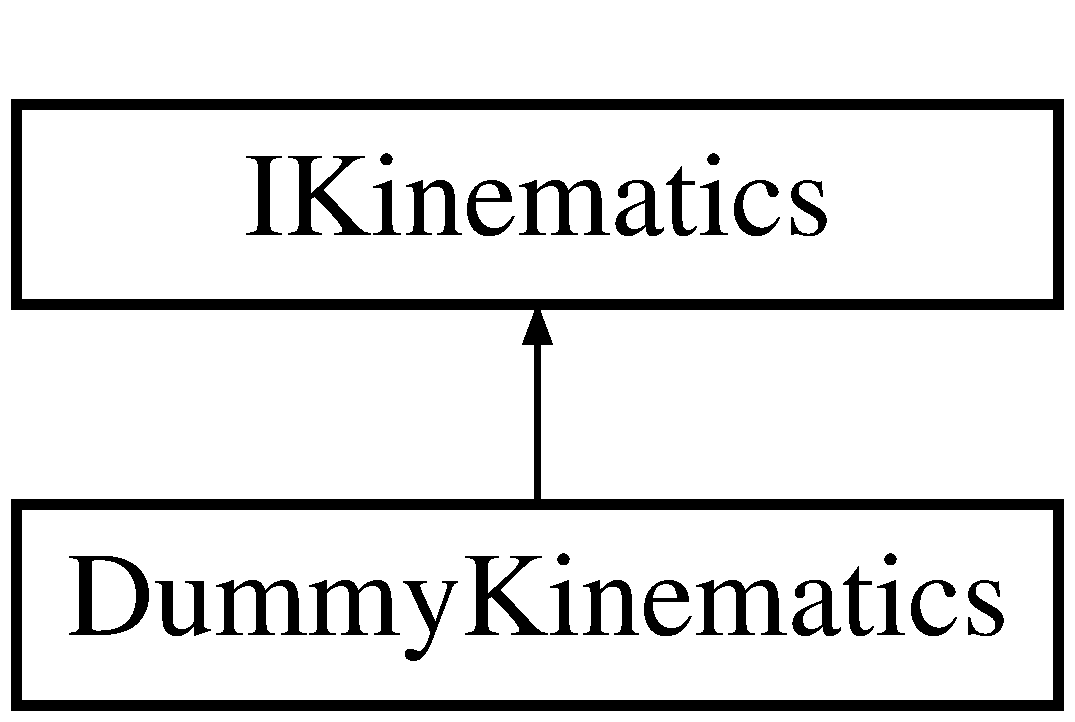
\includegraphics[height=2.000000cm]{classDummyKinematics}
\end{center}
\end{figure}
\subsection*{Public Member Functions}
\begin{DoxyCompactItemize}
\item 
virtual std\-::vector$<$ double $>$ \hyperlink{classDummyKinematics_a630b1a37d23881be53147c07a87bffad}{Get\-Joint\-Values} ()
\item 
virtual void \hyperlink{classDummyKinematics_a0b5a581fb840f304cebc80fb00eb7138}{Set\-Joint\-Values} (std\-::vector$<$ double $>$ joint\-\_\-values)
\item 
virtual urdf\-::\-Pose \hyperlink{classDummyKinematics_a6b69b528361a7f7654f1fa4ba9c019fb}{F\-K} (std\-::vector$<$ double $>$ jv)
\item 
virtual std\-::vector$<$ double $>$ \hyperlink{classDummyKinematics_aed9dcd58e607ccfef58975040567a04a}{I\-K} (\hyperlink{namespaceRCS_aac02c0fd845140ea93a2a9254b1db6f6}{R\-C\-S\-::\-Pose} \&pose, std\-::vector$<$ double $>$ oldjoints)
\item 
virtual size\-\_\-t \hyperlink{classDummyKinematics_ac96c0c98a0ca7847ae38152c6de17d1c}{All\-Pose\-To\-Joints} (\hyperlink{namespaceRCS_aac02c0fd845140ea93a2a9254b1db6f6}{R\-C\-S\-::\-Pose} \&pose, std\-::vector$<$ std\-::vector$<$ double $>$ $>$ \&newjoints)
\item 
virtual std\-::vector$<$ double $>$ \hyperlink{classDummyKinematics_a5069cce91772b48d105065f12f6e15bc}{Nearest\-Joints} (std\-::vector$<$ double $>$ oldjoints, std\-::vector$<$ std\-::vector$<$ double $>$ $>$ \&newjoints)
\end{DoxyCompactItemize}


\subsection{Member Function Documentation}
\hypertarget{classDummyKinematics_ac96c0c98a0ca7847ae38152c6de17d1c}{\index{Dummy\-Kinematics@{Dummy\-Kinematics}!All\-Pose\-To\-Joints@{All\-Pose\-To\-Joints}}
\index{All\-Pose\-To\-Joints@{All\-Pose\-To\-Joints}!DummyKinematics@{Dummy\-Kinematics}}
\subsubsection[{All\-Pose\-To\-Joints}]{\setlength{\rightskip}{0pt plus 5cm}virtual size\-\_\-t Dummy\-Kinematics\-::\-All\-Pose\-To\-Joints (
\begin{DoxyParamCaption}
\item[{{\bf R\-C\-S\-::\-Pose} \&}]{pose, }
\item[{std\-::vector$<$ std\-::vector$<$ double $>$ $>$ \&}]{newjoints}
\end{DoxyParamCaption}
)\hspace{0.3cm}{\ttfamily [inline]}, {\ttfamily [virtual]}}}\label{classDummyKinematics_ac96c0c98a0ca7847ae38152c6de17d1c}


Implements \hyperlink{classIKinematics_aeb53bb4b2a1e70a79d5d724e5eb82c10}{I\-Kinematics}.

\hypertarget{classDummyKinematics_a6b69b528361a7f7654f1fa4ba9c019fb}{\index{Dummy\-Kinematics@{Dummy\-Kinematics}!F\-K@{F\-K}}
\index{F\-K@{F\-K}!DummyKinematics@{Dummy\-Kinematics}}
\subsubsection[{F\-K}]{\setlength{\rightskip}{0pt plus 5cm}virtual urdf\-::\-Pose Dummy\-Kinematics\-::\-F\-K (
\begin{DoxyParamCaption}
\item[{std\-::vector$<$ double $>$}]{jv}
\end{DoxyParamCaption}
)\hspace{0.3cm}{\ttfamily [inline]}, {\ttfamily [virtual]}}}\label{classDummyKinematics_a6b69b528361a7f7654f1fa4ba9c019fb}


Implements \hyperlink{classIKinematics_a377f817ce25355513b518491436150fc}{I\-Kinematics}.

\hypertarget{classDummyKinematics_a630b1a37d23881be53147c07a87bffad}{\index{Dummy\-Kinematics@{Dummy\-Kinematics}!Get\-Joint\-Values@{Get\-Joint\-Values}}
\index{Get\-Joint\-Values@{Get\-Joint\-Values}!DummyKinematics@{Dummy\-Kinematics}}
\subsubsection[{Get\-Joint\-Values}]{\setlength{\rightskip}{0pt plus 5cm}virtual std\-::vector$<$double$>$ Dummy\-Kinematics\-::\-Get\-Joint\-Values (
\begin{DoxyParamCaption}
{}
\end{DoxyParamCaption}
)\hspace{0.3cm}{\ttfamily [inline]}, {\ttfamily [virtual]}}}\label{classDummyKinematics_a630b1a37d23881be53147c07a87bffad}


Implements \hyperlink{classIKinematics_af41a85f8dc0cac9d94f982c7cf58b475}{I\-Kinematics}.

\hypertarget{classDummyKinematics_aed9dcd58e607ccfef58975040567a04a}{\index{Dummy\-Kinematics@{Dummy\-Kinematics}!I\-K@{I\-K}}
\index{I\-K@{I\-K}!DummyKinematics@{Dummy\-Kinematics}}
\subsubsection[{I\-K}]{\setlength{\rightskip}{0pt plus 5cm}virtual std\-::vector$<$double$>$ Dummy\-Kinematics\-::\-I\-K (
\begin{DoxyParamCaption}
\item[{{\bf R\-C\-S\-::\-Pose} \&}]{pose, }
\item[{std\-::vector$<$ double $>$}]{oldjoints}
\end{DoxyParamCaption}
)\hspace{0.3cm}{\ttfamily [inline]}, {\ttfamily [virtual]}}}\label{classDummyKinematics_aed9dcd58e607ccfef58975040567a04a}


Implements \hyperlink{classIKinematics_ad0715c776a7eb325d2543bc34fa8114f}{I\-Kinematics}.

\hypertarget{classDummyKinematics_a5069cce91772b48d105065f12f6e15bc}{\index{Dummy\-Kinematics@{Dummy\-Kinematics}!Nearest\-Joints@{Nearest\-Joints}}
\index{Nearest\-Joints@{Nearest\-Joints}!DummyKinematics@{Dummy\-Kinematics}}
\subsubsection[{Nearest\-Joints}]{\setlength{\rightskip}{0pt plus 5cm}virtual std\-::vector$<$double$>$ Dummy\-Kinematics\-::\-Nearest\-Joints (
\begin{DoxyParamCaption}
\item[{std\-::vector$<$ double $>$}]{oldjoints, }
\item[{std\-::vector$<$ std\-::vector$<$ double $>$ $>$ \&}]{newjoints}
\end{DoxyParamCaption}
)\hspace{0.3cm}{\ttfamily [inline]}, {\ttfamily [virtual]}}}\label{classDummyKinematics_a5069cce91772b48d105065f12f6e15bc}


Implements \hyperlink{classIKinematics_ab74b70ed6ecc53adfc36505b8dd1fef4}{I\-Kinematics}.

\hypertarget{classDummyKinematics_a0b5a581fb840f304cebc80fb00eb7138}{\index{Dummy\-Kinematics@{Dummy\-Kinematics}!Set\-Joint\-Values@{Set\-Joint\-Values}}
\index{Set\-Joint\-Values@{Set\-Joint\-Values}!DummyKinematics@{Dummy\-Kinematics}}
\subsubsection[{Set\-Joint\-Values}]{\setlength{\rightskip}{0pt plus 5cm}virtual void Dummy\-Kinematics\-::\-Set\-Joint\-Values (
\begin{DoxyParamCaption}
\item[{std\-::vector$<$ double $>$}]{joint\-\_\-values}
\end{DoxyParamCaption}
)\hspace{0.3cm}{\ttfamily [inline]}, {\ttfamily [virtual]}}}\label{classDummyKinematics_a0b5a581fb840f304cebc80fb00eb7138}


Implements \hyperlink{classIKinematics_ad43b2185f06e20eb0bf9d5a94d4aec18}{I\-Kinematics}.



The documentation for this class was generated from the following file\-:\begin{DoxyCompactItemize}
\item 
/home/michalos/catkin\-\_\-ws/src/nist\-\_\-fanuc/include/nist\-\_\-fanuc/\hyperlink{Kinematics_8h}{Kinematics.\-h}\end{DoxyCompactItemize}

\hypertarget{structCrcl_1_1GripperStatus}{\section{Crcl\-:\-:Gripper\-Status Struct Reference}
\label{structCrcl_1_1GripperStatus}\index{Crcl\-::\-Gripper\-Status@{Crcl\-::\-Gripper\-Status}}
}


\hyperlink{structCrcl_1_1GripperStatus}{Gripper\-Status} dummy class for future gripper information.  




{\ttfamily \#include $<$crcl.\-h$>$}

\subsection*{Public Attributes}
\begin{DoxyCompactItemize}
\item 
std\-::string \hyperlink{structCrcl_1_1GripperStatus_aa6975369bf9c1d3b7711940d8dd7441d}{\-\_\-name}
\item 
double \hyperlink{structCrcl_1_1GripperStatus_a206c61416e52e3b758130c6068545cb0}{\-\_\-d\-Position}
\end{DoxyCompactItemize}


\subsection{Detailed Description}
\hyperlink{structCrcl_1_1GripperStatus}{Gripper\-Status} dummy class for future gripper information. 

\subsection{Member Data Documentation}
\hypertarget{structCrcl_1_1GripperStatus_a206c61416e52e3b758130c6068545cb0}{\index{Crcl\-::\-Gripper\-Status@{Crcl\-::\-Gripper\-Status}!\-\_\-d\-Position@{\-\_\-d\-Position}}
\index{\-\_\-d\-Position@{\-\_\-d\-Position}!Crcl::GripperStatus@{Crcl\-::\-Gripper\-Status}}
\subsubsection[{\-\_\-d\-Position}]{\setlength{\rightskip}{0pt plus 5cm}double Crcl\-::\-Gripper\-Status\-::\-\_\-d\-Position}}\label{structCrcl_1_1GripperStatus_a206c61416e52e3b758130c6068545cb0}
\hypertarget{structCrcl_1_1GripperStatus_aa6975369bf9c1d3b7711940d8dd7441d}{\index{Crcl\-::\-Gripper\-Status@{Crcl\-::\-Gripper\-Status}!\-\_\-name@{\-\_\-name}}
\index{\-\_\-name@{\-\_\-name}!Crcl::GripperStatus@{Crcl\-::\-Gripper\-Status}}
\subsubsection[{\-\_\-name}]{\setlength{\rightskip}{0pt plus 5cm}std\-::string Crcl\-::\-Gripper\-Status\-::\-\_\-name}}\label{structCrcl_1_1GripperStatus_aa6975369bf9c1d3b7711940d8dd7441d}


The documentation for this struct was generated from the following file\-:\begin{DoxyCompactItemize}
\item 
/home/michalos/catkin\-\_\-ws/src/nist\-\_\-fanuc/include/nist\-\_\-fanuc/\hyperlink{crcl_8h}{crcl.\-h}\end{DoxyCompactItemize}

\hypertarget{classIKinematics}{\section{I\-Kinematics Class Reference}
\label{classIKinematics}\index{I\-Kinematics@{I\-Kinematics}}
}


The \hyperlink{classIKinematics}{I\-Kinematics} provides is an abstract class with pure virtual functions that are overriden by actual kinematic implementations.  




{\ttfamily \#include $<$Kinematics.\-h$>$}

Inheritance diagram for I\-Kinematics\-:\begin{figure}[H]
\begin{center}
\leavevmode
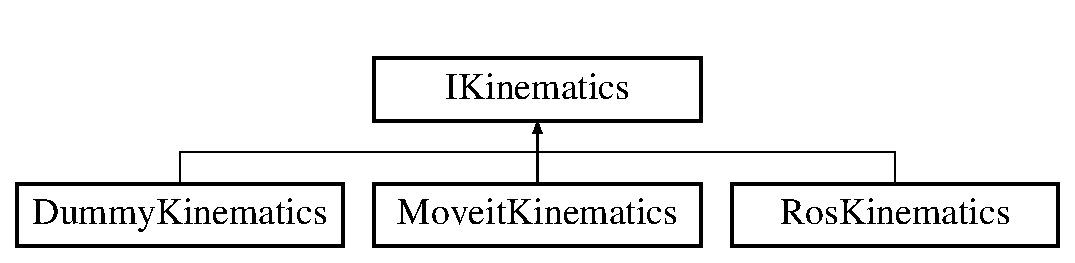
\includegraphics[height=2.000000cm]{classIKinematics}
\end{center}
\end{figure}
\subsection*{Public Member Functions}
\begin{DoxyCompactItemize}
\item 
virtual std\-::vector$<$ double $>$ \hyperlink{classIKinematics_af41a85f8dc0cac9d94f982c7cf58b475}{Get\-Joint\-Values} ()=0
\item 
virtual void \hyperlink{classIKinematics_ad43b2185f06e20eb0bf9d5a94d4aec18}{Set\-Joint\-Values} (std\-::vector$<$ double $>$ joint\-\_\-values)=0
\item 
virtual urdf\-::\-Pose \hyperlink{classIKinematics_a377f817ce25355513b518491436150fc}{F\-K} (std\-::vector$<$ double $>$ jv)=0
\item 
virtual std\-::vector$<$ double $>$ \hyperlink{classIKinematics_ad0715c776a7eb325d2543bc34fa8114f}{I\-K} (\hyperlink{namespaceRCS_aac02c0fd845140ea93a2a9254b1db6f6}{R\-C\-S\-::\-Pose} \&pose, std\-::vector$<$ double $>$ oldjoints)=0
\item 
virtual size\-\_\-t \hyperlink{classIKinematics_aeb53bb4b2a1e70a79d5d724e5eb82c10}{All\-Pose\-To\-Joints} (\hyperlink{namespaceRCS_aac02c0fd845140ea93a2a9254b1db6f6}{R\-C\-S\-::\-Pose} \&pose, std\-::vector$<$ std\-::vector$<$ double $>$ $>$ \&newjoints)=0
\item 
virtual std\-::vector$<$ double $>$ \hyperlink{classIKinematics_ab74b70ed6ecc53adfc36505b8dd1fef4}{Nearest\-Joints} (std\-::vector$<$ double $>$ oldjoints, std\-::vector$<$ std\-::vector$<$ double $>$ $>$ \&newjoints)=0
\item 
virtual void \hyperlink{classIKinematics_a1407620d6cf7f26e61a64af42d570b8f}{Init} (std\-::string groupname, std\-::string eelinkname)
\end{DoxyCompactItemize}


\subsection{Detailed Description}
The \hyperlink{classIKinematics}{I\-Kinematics} provides is an abstract class with pure virtual functions that are overriden by actual kinematic implementations. 

\subsection{Member Function Documentation}
\hypertarget{classIKinematics_aeb53bb4b2a1e70a79d5d724e5eb82c10}{\index{I\-Kinematics@{I\-Kinematics}!All\-Pose\-To\-Joints@{All\-Pose\-To\-Joints}}
\index{All\-Pose\-To\-Joints@{All\-Pose\-To\-Joints}!IKinematics@{I\-Kinematics}}
\subsubsection[{All\-Pose\-To\-Joints}]{\setlength{\rightskip}{0pt plus 5cm}virtual size\-\_\-t I\-Kinematics\-::\-All\-Pose\-To\-Joints (
\begin{DoxyParamCaption}
\item[{{\bf R\-C\-S\-::\-Pose} \&}]{pose, }
\item[{std\-::vector$<$ std\-::vector$<$ double $>$ $>$ \&}]{newjoints}
\end{DoxyParamCaption}
)\hspace{0.3cm}{\ttfamily [pure virtual]}}}\label{classIKinematics_aeb53bb4b2a1e70a79d5d724e5eb82c10}


Implemented in \hyperlink{classMoveitKinematics_a256bfc139809c215c34112a38938a372}{Moveit\-Kinematics}, \hyperlink{classRosKinematics_ae3d78b75e8cbd38a12d451e0e0e95548}{Ros\-Kinematics}, and \hyperlink{classDummyKinematics_ac96c0c98a0ca7847ae38152c6de17d1c}{Dummy\-Kinematics}.

\hypertarget{classIKinematics_a377f817ce25355513b518491436150fc}{\index{I\-Kinematics@{I\-Kinematics}!F\-K@{F\-K}}
\index{F\-K@{F\-K}!IKinematics@{I\-Kinematics}}
\subsubsection[{F\-K}]{\setlength{\rightskip}{0pt plus 5cm}virtual urdf\-::\-Pose I\-Kinematics\-::\-F\-K (
\begin{DoxyParamCaption}
\item[{std\-::vector$<$ double $>$}]{jv}
\end{DoxyParamCaption}
)\hspace{0.3cm}{\ttfamily [pure virtual]}}}\label{classIKinematics_a377f817ce25355513b518491436150fc}


Implemented in \hyperlink{classMoveitKinematics_a530fd2f88c75df40248a24c55081e1eb}{Moveit\-Kinematics}, \hyperlink{classRosKinematics_ac892e14e3d6b14efbc4908404cd9e706}{Ros\-Kinematics}, and \hyperlink{classDummyKinematics_a6b69b528361a7f7654f1fa4ba9c019fb}{Dummy\-Kinematics}.

\hypertarget{classIKinematics_af41a85f8dc0cac9d94f982c7cf58b475}{\index{I\-Kinematics@{I\-Kinematics}!Get\-Joint\-Values@{Get\-Joint\-Values}}
\index{Get\-Joint\-Values@{Get\-Joint\-Values}!IKinematics@{I\-Kinematics}}
\subsubsection[{Get\-Joint\-Values}]{\setlength{\rightskip}{0pt plus 5cm}virtual std\-::vector$<$double$>$ I\-Kinematics\-::\-Get\-Joint\-Values (
\begin{DoxyParamCaption}
{}
\end{DoxyParamCaption}
)\hspace{0.3cm}{\ttfamily [pure virtual]}}}\label{classIKinematics_af41a85f8dc0cac9d94f982c7cf58b475}


Implemented in \hyperlink{classMoveitKinematics_a8f186684d000616a6ff805fa0f41151e}{Moveit\-Kinematics}, \hyperlink{classRosKinematics_ab3e293c7f5d7220fa7ee91256321ec92}{Ros\-Kinematics}, and \hyperlink{classDummyKinematics_a630b1a37d23881be53147c07a87bffad}{Dummy\-Kinematics}.

\hypertarget{classIKinematics_ad0715c776a7eb325d2543bc34fa8114f}{\index{I\-Kinematics@{I\-Kinematics}!I\-K@{I\-K}}
\index{I\-K@{I\-K}!IKinematics@{I\-Kinematics}}
\subsubsection[{I\-K}]{\setlength{\rightskip}{0pt plus 5cm}virtual std\-::vector$<$double$>$ I\-Kinematics\-::\-I\-K (
\begin{DoxyParamCaption}
\item[{{\bf R\-C\-S\-::\-Pose} \&}]{pose, }
\item[{std\-::vector$<$ double $>$}]{oldjoints}
\end{DoxyParamCaption}
)\hspace{0.3cm}{\ttfamily [pure virtual]}}}\label{classIKinematics_ad0715c776a7eb325d2543bc34fa8114f}


Implemented in \hyperlink{classMoveitKinematics_a70fa6e222157b71b6bf8fa7ed33075cc}{Moveit\-Kinematics}, \hyperlink{classRosKinematics_ae8f76a870595ca94d3876bbe51c7b142}{Ros\-Kinematics}, and \hyperlink{classDummyKinematics_aed9dcd58e607ccfef58975040567a04a}{Dummy\-Kinematics}.

\hypertarget{classIKinematics_a1407620d6cf7f26e61a64af42d570b8f}{\index{I\-Kinematics@{I\-Kinematics}!Init@{Init}}
\index{Init@{Init}!IKinematics@{I\-Kinematics}}
\subsubsection[{Init}]{\setlength{\rightskip}{0pt plus 5cm}virtual void I\-Kinematics\-::\-Init (
\begin{DoxyParamCaption}
\item[{std\-::string}]{groupname, }
\item[{std\-::string}]{eelinkname}
\end{DoxyParamCaption}
)\hspace{0.3cm}{\ttfamily [inline]}, {\ttfamily [virtual]}}}\label{classIKinematics_a1407620d6cf7f26e61a64af42d570b8f}


Reimplemented in \hyperlink{classMoveitKinematics_a3d0a3d9eadca26b5a24dd9904fee6e91}{Moveit\-Kinematics}, and \hyperlink{classRosKinematics_a307da5d4456621c4cc2dce412be30db3}{Ros\-Kinematics}.

\hypertarget{classIKinematics_ab74b70ed6ecc53adfc36505b8dd1fef4}{\index{I\-Kinematics@{I\-Kinematics}!Nearest\-Joints@{Nearest\-Joints}}
\index{Nearest\-Joints@{Nearest\-Joints}!IKinematics@{I\-Kinematics}}
\subsubsection[{Nearest\-Joints}]{\setlength{\rightskip}{0pt plus 5cm}virtual std\-::vector$<$double$>$ I\-Kinematics\-::\-Nearest\-Joints (
\begin{DoxyParamCaption}
\item[{std\-::vector$<$ double $>$}]{oldjoints, }
\item[{std\-::vector$<$ std\-::vector$<$ double $>$ $>$ \&}]{newjoints}
\end{DoxyParamCaption}
)\hspace{0.3cm}{\ttfamily [pure virtual]}}}\label{classIKinematics_ab74b70ed6ecc53adfc36505b8dd1fef4}


Implemented in \hyperlink{classMoveitKinematics_acd060eacf93c71b0cfb61bd5c93ceb77}{Moveit\-Kinematics}, \hyperlink{classRosKinematics_ab50d3e7666cf3b2bdb1ae3d5e0a7db8e}{Ros\-Kinematics}, and \hyperlink{classDummyKinematics_a5069cce91772b48d105065f12f6e15bc}{Dummy\-Kinematics}.

\hypertarget{classIKinematics_ad43b2185f06e20eb0bf9d5a94d4aec18}{\index{I\-Kinematics@{I\-Kinematics}!Set\-Joint\-Values@{Set\-Joint\-Values}}
\index{Set\-Joint\-Values@{Set\-Joint\-Values}!IKinematics@{I\-Kinematics}}
\subsubsection[{Set\-Joint\-Values}]{\setlength{\rightskip}{0pt plus 5cm}virtual void I\-Kinematics\-::\-Set\-Joint\-Values (
\begin{DoxyParamCaption}
\item[{std\-::vector$<$ double $>$}]{joint\-\_\-values}
\end{DoxyParamCaption}
)\hspace{0.3cm}{\ttfamily [pure virtual]}}}\label{classIKinematics_ad43b2185f06e20eb0bf9d5a94d4aec18}


Implemented in \hyperlink{classMoveitKinematics_aee274ed4deddecb36191f8711c4b7c2e}{Moveit\-Kinematics}, \hyperlink{classRosKinematics_af9af8957f54e5d2343b2ab00dcb55525}{Ros\-Kinematics}, and \hyperlink{classDummyKinematics_a0b5a581fb840f304cebc80fb00eb7138}{Dummy\-Kinematics}.



The documentation for this class was generated from the following file\-:\begin{DoxyCompactItemize}
\item 
/home/michalos/catkin\-\_\-ws/src/nist\-\_\-fanuc/include/nist\-\_\-fanuc/\hyperlink{Kinematics_8h}{Kinematics.\-h}\end{DoxyCompactItemize}

\hypertarget{classIRate}{\section{I\-Rate Class Reference}
\label{classIRate}\index{I\-Rate@{I\-Rate}}
}


\hyperlink{classIRate}{I\-Rate} is an interface class for defining the allowed motion rates.  




{\ttfamily \#include $<$trajectory\-Maker.\-h$>$}

\subsection*{Public Member Functions}
\begin{DoxyCompactItemize}
\item 
\hyperlink{classIRate_a4cc7acdfa6770b7a28b3be6ec90110d9}{I\-Rate} ()
\item 
\hyperlink{classIRate_ab2d1966894aa6d963a20f5e6d18097de}{I\-Rate} (double maximum\-\_\-velocity, double maximum\-\_\-accel, double cycle\-Time)
\item 
void \hyperlink{classIRate_a9a6f938787dd958daef0f8eb2c0836fc}{Set\-Current\-Motion} (double final\-\_\-velocity, double current\-\_\-feedrate, double current\-\_\-velocity)
\item 
\hyperlink{classIRate_ad20f3c10a92de570de814b8c33c55813}{N\-V\-A\-R} (Final\-Velocity, double, \-\_\-final\-\_\-velocity)
\item 
\hyperlink{classIRate_ac083b3315892fb042e0240fa37635405}{N\-V\-A\-R} (Current\-Feedrate, double, \-\_\-current\-\_\-feedrate)
\item 
\hyperlink{classIRate_a52f26275fc49b2fd4c5b69291185a6db}{N\-V\-A\-R} (Current\-Velocity, double, \-\_\-current\-\_\-velocity)
\item 
\hyperlink{classIRate_a26f1529cb8c8cc9694ae82ed8e153563}{N\-V\-A\-R} (Maximum\-Velocity, double, \-\_\-maximum\-\_\-velocity)
\item 
\hyperlink{classIRate_aa338ed93323d145c8eb4e656625e9333}{N\-V\-A\-R} (Maximum\-Accel, double, \-\_\-maximum\-\_\-accel)
\item 
\hyperlink{classIRate_a9292518c87c8e371ba55b6aa49ad1706}{N\-V\-A\-R} (Cycle\-Time, double, \-\_\-cycle\-Time)
\item 
\hyperlink{classIRate_ac6149473cf0f8e1e6d90255e8da44e89}{N\-V\-A\-R} (Current\-Accel, double, \-\_\-current\-\_\-accel)
\item 
\hyperlink{classIRate_a6555656cff42f8e9f6e633876db9b6c1}{N\-V\-A\-R} (Ms\-Flag, \hyperlink{namespaceRCS_a452a9217023e577031dcdf7e533b2ead}{R\-C\-S\-::\-Canon\-Acc\-Profile}, \-\_\-msflag)
\end{DoxyCompactItemize}


\subsection{Detailed Description}
\hyperlink{classIRate}{I\-Rate} is an interface class for defining the allowed motion rates. 

\subsection{Constructor \& Destructor Documentation}
\hypertarget{classIRate_a4cc7acdfa6770b7a28b3be6ec90110d9}{\index{I\-Rate@{I\-Rate}!I\-Rate@{I\-Rate}}
\index{I\-Rate@{I\-Rate}!IRate@{I\-Rate}}
\subsubsection[{I\-Rate}]{\setlength{\rightskip}{0pt plus 5cm}I\-Rate\-::\-I\-Rate (
\begin{DoxyParamCaption}
{}
\end{DoxyParamCaption}
)\hspace{0.3cm}{\ttfamily [inline]}}}\label{classIRate_a4cc7acdfa6770b7a28b3be6ec90110d9}
\hypertarget{classIRate_ab2d1966894aa6d963a20f5e6d18097de}{\index{I\-Rate@{I\-Rate}!I\-Rate@{I\-Rate}}
\index{I\-Rate@{I\-Rate}!IRate@{I\-Rate}}
\subsubsection[{I\-Rate}]{\setlength{\rightskip}{0pt plus 5cm}I\-Rate\-::\-I\-Rate (
\begin{DoxyParamCaption}
\item[{double}]{maximum\-\_\-velocity, }
\item[{double}]{maximum\-\_\-accel, }
\item[{double}]{cycle\-Time}
\end{DoxyParamCaption}
)\hspace{0.3cm}{\ttfamily [inline]}}}\label{classIRate_ab2d1966894aa6d963a20f5e6d18097de}


\subsection{Member Function Documentation}
\hypertarget{classIRate_ad20f3c10a92de570de814b8c33c55813}{\index{I\-Rate@{I\-Rate}!N\-V\-A\-R@{N\-V\-A\-R}}
\index{N\-V\-A\-R@{N\-V\-A\-R}!IRate@{I\-Rate}}
\subsubsection[{N\-V\-A\-R}]{\setlength{\rightskip}{0pt plus 5cm}I\-Rate\-::\-N\-V\-A\-R (
\begin{DoxyParamCaption}
\item[{Final\-Velocity}]{, }
\item[{double}]{, }
\item[{\-\_\-final\-\_\-velocity}]{}
\end{DoxyParamCaption}
)}}\label{classIRate_ad20f3c10a92de570de814b8c33c55813}
\hypertarget{classIRate_ac083b3315892fb042e0240fa37635405}{\index{I\-Rate@{I\-Rate}!N\-V\-A\-R@{N\-V\-A\-R}}
\index{N\-V\-A\-R@{N\-V\-A\-R}!IRate@{I\-Rate}}
\subsubsection[{N\-V\-A\-R}]{\setlength{\rightskip}{0pt plus 5cm}I\-Rate\-::\-N\-V\-A\-R (
\begin{DoxyParamCaption}
\item[{Current\-Feedrate}]{, }
\item[{double}]{, }
\item[{\-\_\-current\-\_\-feedrate}]{}
\end{DoxyParamCaption}
)}}\label{classIRate_ac083b3315892fb042e0240fa37635405}
\hypertarget{classIRate_a52f26275fc49b2fd4c5b69291185a6db}{\index{I\-Rate@{I\-Rate}!N\-V\-A\-R@{N\-V\-A\-R}}
\index{N\-V\-A\-R@{N\-V\-A\-R}!IRate@{I\-Rate}}
\subsubsection[{N\-V\-A\-R}]{\setlength{\rightskip}{0pt plus 5cm}I\-Rate\-::\-N\-V\-A\-R (
\begin{DoxyParamCaption}
\item[{Current\-Velocity}]{, }
\item[{double}]{, }
\item[{\-\_\-current\-\_\-velocity}]{}
\end{DoxyParamCaption}
)}}\label{classIRate_a52f26275fc49b2fd4c5b69291185a6db}
\hypertarget{classIRate_a26f1529cb8c8cc9694ae82ed8e153563}{\index{I\-Rate@{I\-Rate}!N\-V\-A\-R@{N\-V\-A\-R}}
\index{N\-V\-A\-R@{N\-V\-A\-R}!IRate@{I\-Rate}}
\subsubsection[{N\-V\-A\-R}]{\setlength{\rightskip}{0pt plus 5cm}I\-Rate\-::\-N\-V\-A\-R (
\begin{DoxyParamCaption}
\item[{Maximum\-Velocity}]{, }
\item[{double}]{, }
\item[{\-\_\-maximum\-\_\-velocity}]{}
\end{DoxyParamCaption}
)}}\label{classIRate_a26f1529cb8c8cc9694ae82ed8e153563}
\hypertarget{classIRate_aa338ed93323d145c8eb4e656625e9333}{\index{I\-Rate@{I\-Rate}!N\-V\-A\-R@{N\-V\-A\-R}}
\index{N\-V\-A\-R@{N\-V\-A\-R}!IRate@{I\-Rate}}
\subsubsection[{N\-V\-A\-R}]{\setlength{\rightskip}{0pt plus 5cm}I\-Rate\-::\-N\-V\-A\-R (
\begin{DoxyParamCaption}
\item[{Maximum\-Accel}]{, }
\item[{double}]{, }
\item[{\-\_\-maximum\-\_\-accel}]{}
\end{DoxyParamCaption}
)}}\label{classIRate_aa338ed93323d145c8eb4e656625e9333}
\hypertarget{classIRate_a9292518c87c8e371ba55b6aa49ad1706}{\index{I\-Rate@{I\-Rate}!N\-V\-A\-R@{N\-V\-A\-R}}
\index{N\-V\-A\-R@{N\-V\-A\-R}!IRate@{I\-Rate}}
\subsubsection[{N\-V\-A\-R}]{\setlength{\rightskip}{0pt plus 5cm}I\-Rate\-::\-N\-V\-A\-R (
\begin{DoxyParamCaption}
\item[{Cycle\-Time}]{, }
\item[{double}]{, }
\item[{\-\_\-cycle\-Time}]{}
\end{DoxyParamCaption}
)}}\label{classIRate_a9292518c87c8e371ba55b6aa49ad1706}
\hypertarget{classIRate_ac6149473cf0f8e1e6d90255e8da44e89}{\index{I\-Rate@{I\-Rate}!N\-V\-A\-R@{N\-V\-A\-R}}
\index{N\-V\-A\-R@{N\-V\-A\-R}!IRate@{I\-Rate}}
\subsubsection[{N\-V\-A\-R}]{\setlength{\rightskip}{0pt plus 5cm}I\-Rate\-::\-N\-V\-A\-R (
\begin{DoxyParamCaption}
\item[{Current\-Accel}]{, }
\item[{double}]{, }
\item[{\-\_\-current\-\_\-accel}]{}
\end{DoxyParamCaption}
)}}\label{classIRate_ac6149473cf0f8e1e6d90255e8da44e89}
\hypertarget{classIRate_a6555656cff42f8e9f6e633876db9b6c1}{\index{I\-Rate@{I\-Rate}!N\-V\-A\-R@{N\-V\-A\-R}}
\index{N\-V\-A\-R@{N\-V\-A\-R}!IRate@{I\-Rate}}
\subsubsection[{N\-V\-A\-R}]{\setlength{\rightskip}{0pt plus 5cm}I\-Rate\-::\-N\-V\-A\-R (
\begin{DoxyParamCaption}
\item[{Ms\-Flag}]{, }
\item[{{\bf R\-C\-S\-::\-Canon\-Acc\-Profile}}]{, }
\item[{\-\_\-msflag}]{}
\end{DoxyParamCaption}
)}}\label{classIRate_a6555656cff42f8e9f6e633876db9b6c1}
\hypertarget{classIRate_a9a6f938787dd958daef0f8eb2c0836fc}{\index{I\-Rate@{I\-Rate}!Set\-Current\-Motion@{Set\-Current\-Motion}}
\index{Set\-Current\-Motion@{Set\-Current\-Motion}!IRate@{I\-Rate}}
\subsubsection[{Set\-Current\-Motion}]{\setlength{\rightskip}{0pt plus 5cm}void I\-Rate\-::\-Set\-Current\-Motion (
\begin{DoxyParamCaption}
\item[{double}]{final\-\_\-velocity, }
\item[{double}]{current\-\_\-feedrate, }
\item[{double}]{current\-\_\-velocity}
\end{DoxyParamCaption}
)\hspace{0.3cm}{\ttfamily [inline]}}}\label{classIRate_a9a6f938787dd958daef0f8eb2c0836fc}


The documentation for this class was generated from the following file\-:\begin{DoxyCompactItemize}
\item 
/home/michalos/catkin\-\_\-ws/src/nist\-\_\-fanuc/include/nist\-\_\-fanuc/\hyperlink{trajectoryMaker_8h}{trajectory\-Maker.\-h}\end{DoxyCompactItemize}

\hypertarget{structCrcl_1_1JointReport}{\section{Crcl\-:\-:Joint\-Report Struct Reference}
\label{structCrcl_1_1JointReport}\index{Crcl\-::\-Joint\-Report@{Crcl\-::\-Joint\-Report}}
}


{\ttfamily \#include $<$crcl.\-h$>$}

\subsection*{Public Attributes}
\begin{DoxyCompactItemize}
\item 
size\-\_\-t \hyperlink{structCrcl_1_1JointReport_ac49defefe1565597177b1363dec3eb66}{\-\_\-n\-Joint\-Number}
\item 
bool \hyperlink{structCrcl_1_1JointReport_a768a2ddefebd748006d8295f863a2faf}{\-\_\-b\-Report\-Position}
\item 
bool \hyperlink{structCrcl_1_1JointReport_a8688287259bf8e0619a6f4a06a3c5721}{\-\_\-b\-Report\-Torque\-Or\-Force}
\item 
bool \hyperlink{structCrcl_1_1JointReport_aea4383b9bb5263ec07cc151d574442c9}{\-\_\-b\-Report\-Velocity}
\end{DoxyCompactItemize}


\subsection{Member Data Documentation}
\hypertarget{structCrcl_1_1JointReport_a768a2ddefebd748006d8295f863a2faf}{\index{Crcl\-::\-Joint\-Report@{Crcl\-::\-Joint\-Report}!\-\_\-b\-Report\-Position@{\-\_\-b\-Report\-Position}}
\index{\-\_\-b\-Report\-Position@{\-\_\-b\-Report\-Position}!Crcl::JointReport@{Crcl\-::\-Joint\-Report}}
\subsubsection[{\-\_\-b\-Report\-Position}]{\setlength{\rightskip}{0pt plus 5cm}bool Crcl\-::\-Joint\-Report\-::\-\_\-b\-Report\-Position}}\label{structCrcl_1_1JointReport_a768a2ddefebd748006d8295f863a2faf}
\hypertarget{structCrcl_1_1JointReport_a8688287259bf8e0619a6f4a06a3c5721}{\index{Crcl\-::\-Joint\-Report@{Crcl\-::\-Joint\-Report}!\-\_\-b\-Report\-Torque\-Or\-Force@{\-\_\-b\-Report\-Torque\-Or\-Force}}
\index{\-\_\-b\-Report\-Torque\-Or\-Force@{\-\_\-b\-Report\-Torque\-Or\-Force}!Crcl::JointReport@{Crcl\-::\-Joint\-Report}}
\subsubsection[{\-\_\-b\-Report\-Torque\-Or\-Force}]{\setlength{\rightskip}{0pt plus 5cm}bool Crcl\-::\-Joint\-Report\-::\-\_\-b\-Report\-Torque\-Or\-Force}}\label{structCrcl_1_1JointReport_a8688287259bf8e0619a6f4a06a3c5721}
\hypertarget{structCrcl_1_1JointReport_aea4383b9bb5263ec07cc151d574442c9}{\index{Crcl\-::\-Joint\-Report@{Crcl\-::\-Joint\-Report}!\-\_\-b\-Report\-Velocity@{\-\_\-b\-Report\-Velocity}}
\index{\-\_\-b\-Report\-Velocity@{\-\_\-b\-Report\-Velocity}!Crcl::JointReport@{Crcl\-::\-Joint\-Report}}
\subsubsection[{\-\_\-b\-Report\-Velocity}]{\setlength{\rightskip}{0pt plus 5cm}bool Crcl\-::\-Joint\-Report\-::\-\_\-b\-Report\-Velocity}}\label{structCrcl_1_1JointReport_aea4383b9bb5263ec07cc151d574442c9}
\hypertarget{structCrcl_1_1JointReport_ac49defefe1565597177b1363dec3eb66}{\index{Crcl\-::\-Joint\-Report@{Crcl\-::\-Joint\-Report}!\-\_\-n\-Joint\-Number@{\-\_\-n\-Joint\-Number}}
\index{\-\_\-n\-Joint\-Number@{\-\_\-n\-Joint\-Number}!Crcl::JointReport@{Crcl\-::\-Joint\-Report}}
\subsubsection[{\-\_\-n\-Joint\-Number}]{\setlength{\rightskip}{0pt plus 5cm}size\-\_\-t Crcl\-::\-Joint\-Report\-::\-\_\-n\-Joint\-Number}}\label{structCrcl_1_1JointReport_ac49defefe1565597177b1363dec3eb66}


The documentation for this struct was generated from the following file\-:\begin{DoxyCompactItemize}
\item 
/home/michalos/catkin\-\_\-ws/src/nist\-\_\-fanuc/include/nist\-\_\-fanuc/\hyperlink{crcl_8h}{crcl.\-h}\end{DoxyCompactItemize}

\hypertarget{classMotionControl}{\section{Motion\-Control Class Reference}
\label{classMotionControl}\index{Motion\-Control@{Motion\-Control}}
}


\hyperlink{classMotionControl}{Motion\-Control} is a class that contains some useful motion control methods.  




{\ttfamily \#include $<$Motion\-Control.\-h$>$}

\subsection*{Public Member Functions}
\begin{DoxyCompactItemize}
\item 
bool \hyperlink{classMotionControl_a7d4bdb16c10626850dac271d30428f71}{execute\-Trajectory} (const trajectory\-\_\-msgs\-::\-Joint\-Trajectory \&trajectory, const std\-::string \&trajectory\-\_\-ns)
\begin{DoxyCompactList}\small\item\em execute\-Trajectory will send a traject to ros to execute \end{DoxyCompactList}\item 
\hyperlink{namespaceRCS_aa07e45d8a50e30064283d2b38087f999}{R\-C\-S\-::\-Pose} \hyperlink{classMotionControl_a9d242a51b301d7c87c16f579e0d9347e}{compute\-Translation} (\hyperlink{namespaceRCS_aa07e45d8a50e30064283d2b38087f999}{R\-C\-S\-::\-Pose} \&\-\_\-cur\-Pos, \hyperlink{namespaceRCS_aa07e45d8a50e30064283d2b38087f999}{R\-C\-S\-::\-Pose} \&\-\_\-goal\-Pos, double d\-Increment)
\begin{DoxyCompactList}\small\item\em Return linear interpolation (lerp) between current and goal translation. \end{DoxyCompactList}\item 
std\-::vector$<$ \hyperlink{namespaceRCS_aa07e45d8a50e30064283d2b38087f999}{R\-C\-S\-::\-Pose} $>$ \hyperlink{classMotionControl_a40113f305b3accd4d28fa976151aa954}{compute\-Waypoints} (\hyperlink{namespaceRCS_aa07e45d8a50e30064283d2b38087f999}{R\-C\-S\-::\-Pose} \&\-\_\-cur\-Pos, \hyperlink{namespaceRCS_aa07e45d8a50e30064283d2b38087f999}{R\-C\-S\-::\-Pose} \&\-\_\-goal\-Pos, double d\-Gap=0.\-001, bool b\-Add\-Start=false)
\begin{DoxyCompactList}\small\item\em Compute waypoints between current and goal poses with assigned distance between poses. \end{DoxyCompactList}\item 
std\-::vector$<$ \hyperlink{RCS_8h_aa4adb93a26caa4dacba9c9614e283245}{Joint\-State} $>$ \hyperlink{classMotionControl_aebf1d77a70bbf6817f0899a98173b87d}{compute\-Coorindated\-Waypoints} (std\-::vector$<$ double $>$ \&\-\_\-cur\-Jts, std\-::vector$<$ double $>$ \&\-\_\-goal\-Jts, double d\-Gap=0.\-001, bool b\-Add\-Start=false)
\begin{DoxyCompactList}\small\item\em compute\-Coorindated\-Waypoints returns a vector of straightline waypoints between current and goal poses at a given distance. Joints arrive a destination at the same time within the trajectory. \end{DoxyCompactList}\item 
std\-::vector$<$ \hyperlink{RCS_8h_aa4adb93a26caa4dacba9c9614e283245}{Joint\-State} $>$ \hyperlink{classMotionControl_a5a7f01d81030676aab106b7bf4c60aa6}{compute\-Uncoorindated\-Waypoints} (std\-::vector$<$ double $>$ \&\-\_\-cur\-Jts, std\-::vector$<$ double $>$ \&\-\_\-goal\-Jts, double d\-Gap=0.\-001, bool b\-Add\-Start=false)
\begin{DoxyCompactList}\small\item\em compute\-Uncoorindated\-Waypoints returns a vector of waypoints between current and goal poses at a given distance. Joints arrive a destination at various times in the trajectory. \end{DoxyCompactList}\item 
int \hyperlink{classMotionControl_ac065f800e86df7a771aae2aa4271aaa3}{compute\-Increments} (std\-::vector$<$ double $>$ \&\-\_\-cur\-Jts, std\-::vector$<$ double $>$ \&\-\_\-goal\-Jts, double gap=0.\-001)
\item 
int \hyperlink{classMotionControl_a1dbb240abf15324af65904bfba39bd41}{compute\-Increments} (\hyperlink{namespaceRCS_aa07e45d8a50e30064283d2b38087f999}{R\-C\-S\-::\-Pose} \&\-\_\-cur\-Pos, \hyperlink{namespaceRCS_aa07e45d8a50e30064283d2b38087f999}{R\-C\-S\-::\-Pose} \&\-\_\-goal\-Pos, double d\-Gap=0.\-001)
\end{DoxyCompactItemize}
\subsection*{Static Public Member Functions}
\begin{DoxyCompactItemize}
\item 
static bool \hyperlink{classMotionControl_a57fb4b492bc50f10b4fd5e068bda4f7a}{At\-Goal} (\hyperlink{RCS_8h_aa4adb93a26caa4dacba9c9614e283245}{Joint\-State} goal, \hyperlink{RCS_8h_aa4adb93a26caa4dacba9c9614e283245}{Joint\-State} current, double \hyperlink{classMotionControl_ad3cadb7d245794540e4a320ee560b6b2}{epsilon}=0.\-001)
\begin{DoxyCompactList}\small\item\em At\-Goal will determine if a pair joint state values are equal (within an epsilon tolerance). \end{DoxyCompactList}\end{DoxyCompactItemize}
\subsection*{Static Public Attributes}
\begin{DoxyCompactItemize}
\item 
static double \hyperlink{classMotionControl_ad3cadb7d245794540e4a320ee560b6b2}{epsilon} = 0.\-001
\end{DoxyCompactItemize}


\subsection{Detailed Description}
\hyperlink{classMotionControl}{Motion\-Control} is a class that contains some useful motion control methods. 

\subsection{Member Function Documentation}
\hypertarget{classMotionControl_a57fb4b492bc50f10b4fd5e068bda4f7a}{\index{Motion\-Control@{Motion\-Control}!At\-Goal@{At\-Goal}}
\index{At\-Goal@{At\-Goal}!MotionControl@{Motion\-Control}}
\subsubsection[{At\-Goal}]{\setlength{\rightskip}{0pt plus 5cm}bool Motion\-Control\-::\-At\-Goal (
\begin{DoxyParamCaption}
\item[{{\bf Joint\-State}}]{goal, }
\item[{{\bf Joint\-State}}]{current, }
\item[{double}]{epsilon = {\ttfamily 0.001}}
\end{DoxyParamCaption}
)\hspace{0.3cm}{\ttfamily [static]}}}\label{classMotionControl_a57fb4b492bc50f10b4fd5e068bda4f7a}


At\-Goal will determine if a pair joint state values are equal (within an epsilon tolerance). 


\begin{DoxyParams}{Parameters}
{\em goal} & description of goal joint state \\
\hline
{\em current} & description of current joint state \\
\hline
{\em epsilon} & tolerance of equality \\
\hline
\end{DoxyParams}
\begin{DoxyReturn}{Returns}
boolean whether robot is at the desired goal described in joint values. 
\end{DoxyReturn}
\hypertarget{classMotionControl_aebf1d77a70bbf6817f0899a98173b87d}{\index{Motion\-Control@{Motion\-Control}!compute\-Coorindated\-Waypoints@{compute\-Coorindated\-Waypoints}}
\index{compute\-Coorindated\-Waypoints@{compute\-Coorindated\-Waypoints}!MotionControl@{Motion\-Control}}
\subsubsection[{compute\-Coorindated\-Waypoints}]{\setlength{\rightskip}{0pt plus 5cm}std\-::vector$<$ {\bf Joint\-State} $>$ Motion\-Control\-::compute\-Coorindated\-Waypoints (
\begin{DoxyParamCaption}
\item[{std\-::vector$<$ double $>$ \&}]{\-\_\-cur\-Jts, }
\item[{std\-::vector$<$ double $>$ \&}]{\-\_\-goal\-Jts, }
\item[{double}]{d\-Gap = {\ttfamily 0.001}, }
\item[{bool}]{b\-Add\-Start = {\ttfamily false}}
\end{DoxyParamCaption}
)}}\label{classMotionControl_aebf1d77a70bbf6817f0899a98173b87d}


compute\-Coorindated\-Waypoints returns a vector of straightline waypoints between current and goal poses at a given distance. Joints arrive a destination at the same time within the trajectory. 


\begin{DoxyParams}{Parameters}
{\em \-\_\-cur\-Pos} & description of current pose \\
\hline
{\em \-\_\-goal\-Pos} & description of goal pose \\
\hline
{\em gap} & distance between waypoints \\
\hline
{\em b\-Add\-Start} & boolean to determine if starting pose is included in waypoints \\
\hline
\end{DoxyParams}
\begin{DoxyReturn}{Returns}
vector of straighline waypoint poses with gap distance between poses. 
\end{DoxyReturn}
\hypertarget{classMotionControl_ac065f800e86df7a771aae2aa4271aaa3}{\index{Motion\-Control@{Motion\-Control}!compute\-Increments@{compute\-Increments}}
\index{compute\-Increments@{compute\-Increments}!MotionControl@{Motion\-Control}}
\subsubsection[{compute\-Increments}]{\setlength{\rightskip}{0pt plus 5cm}int Motion\-Control\-::compute\-Increments (
\begin{DoxyParamCaption}
\item[{std\-::vector$<$ double $>$ \&}]{\-\_\-cur\-Jts, }
\item[{std\-::vector$<$ double $>$ \&}]{\-\_\-goal\-Jts, }
\item[{double}]{gap = {\ttfamily 0.001}}
\end{DoxyParamCaption}
)}}\label{classMotionControl_ac065f800e86df7a771aae2aa4271aaa3}
\hypertarget{classMotionControl_a1dbb240abf15324af65904bfba39bd41}{\index{Motion\-Control@{Motion\-Control}!compute\-Increments@{compute\-Increments}}
\index{compute\-Increments@{compute\-Increments}!MotionControl@{Motion\-Control}}
\subsubsection[{compute\-Increments}]{\setlength{\rightskip}{0pt plus 5cm}int Motion\-Control\-::compute\-Increments (
\begin{DoxyParamCaption}
\item[{{\bf R\-C\-S\-::\-Pose} \&}]{\-\_\-cur\-Pos, }
\item[{{\bf R\-C\-S\-::\-Pose} \&}]{\-\_\-goal\-Pos, }
\item[{double}]{d\-Gap = {\ttfamily 0.001}}
\end{DoxyParamCaption}
)}}\label{classMotionControl_a1dbb240abf15324af65904bfba39bd41}
\hypertarget{classMotionControl_a9d242a51b301d7c87c16f579e0d9347e}{\index{Motion\-Control@{Motion\-Control}!compute\-Translation@{compute\-Translation}}
\index{compute\-Translation@{compute\-Translation}!MotionControl@{Motion\-Control}}
\subsubsection[{compute\-Translation}]{\setlength{\rightskip}{0pt plus 5cm}{\bf R\-C\-S\-::\-Pose} Motion\-Control\-::compute\-Translation (
\begin{DoxyParamCaption}
\item[{{\bf R\-C\-S\-::\-Pose} \&}]{\-\_\-cur\-Pos, }
\item[{{\bf R\-C\-S\-::\-Pose} \&}]{\-\_\-goal\-Pos, }
\item[{double}]{d\-Increment}
\end{DoxyParamCaption}
)}}\label{classMotionControl_a9d242a51b301d7c87c16f579e0d9347e}


Return linear interpolation (lerp) between current and goal translation. 


\begin{DoxyParams}{Parameters}
{\em \-\_\-cur\-Pos} & description of current pose \\
\hline
{\em \-\_\-goal\-Pos} & description of goal pose \\
\hline
{\em d\-Increment} & translation amount from \mbox{[}0..1\mbox{]} \\
\hline
\end{DoxyParams}
\begin{DoxyReturn}{Returns}
pose containing lerped pose translation. 
\end{DoxyReturn}
\hypertarget{classMotionControl_a5a7f01d81030676aab106b7bf4c60aa6}{\index{Motion\-Control@{Motion\-Control}!compute\-Uncoorindated\-Waypoints@{compute\-Uncoorindated\-Waypoints}}
\index{compute\-Uncoorindated\-Waypoints@{compute\-Uncoorindated\-Waypoints}!MotionControl@{Motion\-Control}}
\subsubsection[{compute\-Uncoorindated\-Waypoints}]{\setlength{\rightskip}{0pt plus 5cm}std\-::vector$<$ {\bf Joint\-State} $>$ Motion\-Control\-::compute\-Uncoorindated\-Waypoints (
\begin{DoxyParamCaption}
\item[{std\-::vector$<$ double $>$ \&}]{\-\_\-cur\-Jts, }
\item[{std\-::vector$<$ double $>$ \&}]{\-\_\-goal\-Jts, }
\item[{double}]{d\-Gap = {\ttfamily 0.001}, }
\item[{bool}]{b\-Add\-Start = {\ttfamily false}}
\end{DoxyParamCaption}
)}}\label{classMotionControl_a5a7f01d81030676aab106b7bf4c60aa6}


compute\-Uncoorindated\-Waypoints returns a vector of waypoints between current and goal poses at a given distance. Joints arrive a destination at various times in the trajectory. 


\begin{DoxyParams}{Parameters}
{\em \-\_\-cur\-Pos} & description of current pose \\
\hline
{\em \-\_\-goal\-Pos} & description of goal pose \\
\hline
{\em gap} & distance between waypoints \\
\hline
{\em b\-Add\-Start} & boolean to determine if starting pose is included in waypoints \\
\hline
\end{DoxyParams}
\begin{DoxyReturn}{Returns}
vector of straighline waypoint poses with gap distance between poses. 
\end{DoxyReturn}
\hypertarget{classMotionControl_a40113f305b3accd4d28fa976151aa954}{\index{Motion\-Control@{Motion\-Control}!compute\-Waypoints@{compute\-Waypoints}}
\index{compute\-Waypoints@{compute\-Waypoints}!MotionControl@{Motion\-Control}}
\subsubsection[{compute\-Waypoints}]{\setlength{\rightskip}{0pt plus 5cm}std\-::vector$<$ {\bf R\-C\-S\-::\-Pose} $>$ Motion\-Control\-::compute\-Waypoints (
\begin{DoxyParamCaption}
\item[{{\bf R\-C\-S\-::\-Pose} \&}]{\-\_\-cur\-Pos, }
\item[{{\bf R\-C\-S\-::\-Pose} \&}]{\-\_\-goal\-Pos, }
\item[{double}]{d\-Gap = {\ttfamily 0.001}, }
\item[{bool}]{b\-Add\-Start = {\ttfamily false}}
\end{DoxyParamCaption}
)}}\label{classMotionControl_a40113f305b3accd4d28fa976151aa954}


Compute waypoints between current and goal poses with assigned distance between poses. 


\begin{DoxyParams}{Parameters}
{\em \-\_\-cur\-Pos} & description of current pose \\
\hline
{\em \-\_\-goal\-Pos} & description of goal pose \\
\hline
{\em gap} & distance between waypoints \\
\hline
{\em b\-Add\-Start} & boolean to determine if starting pose is included in waypoints \\
\hline
\end{DoxyParams}
\begin{DoxyReturn}{Returns}
vector of waypoint poses with gap distance between poses. 
\end{DoxyReturn}
\hypertarget{classMotionControl_a7d4bdb16c10626850dac271d30428f71}{\index{Motion\-Control@{Motion\-Control}!execute\-Trajectory@{execute\-Trajectory}}
\index{execute\-Trajectory@{execute\-Trajectory}!MotionControl@{Motion\-Control}}
\subsubsection[{execute\-Trajectory}]{\setlength{\rightskip}{0pt plus 5cm}bool Motion\-Control\-::execute\-Trajectory (
\begin{DoxyParamCaption}
\item[{const trajectory\-\_\-msgs\-::\-Joint\-Trajectory \&}]{trajectory, }
\item[{const std\-::string \&}]{trajectory\-\_\-ns}
\end{DoxyParamCaption}
)}}\label{classMotionControl_a7d4bdb16c10626850dac271d30428f71}


execute\-Trajectory will send a traject to ros to execute 


\begin{DoxyParams}{Parameters}
{\em trajectory} & \\
\hline
{\em trajectory\-\_\-ns} & namespace of trajectory \\
\hline
\end{DoxyParams}
\begin{DoxyReturn}{Returns}
boolean whether success or failure 
\end{DoxyReturn}


\subsection{Member Data Documentation}
\hypertarget{classMotionControl_ad3cadb7d245794540e4a320ee560b6b2}{\index{Motion\-Control@{Motion\-Control}!epsilon@{epsilon}}
\index{epsilon@{epsilon}!MotionControl@{Motion\-Control}}
\subsubsection[{epsilon}]{\setlength{\rightskip}{0pt plus 5cm}double Motion\-Control\-::epsilon = 0.\-001\hspace{0.3cm}{\ttfamily [static]}}}\label{classMotionControl_ad3cadb7d245794540e4a320ee560b6b2}
allowable difference length in equality between two numbers 

The documentation for this class was generated from the following files\-:\begin{DoxyCompactItemize}
\item 
/usr/local/michalos/github/usnistgov/el-\/robotics-\/core/nist\-\_\-fanuc/include/nist\-\_\-fanuc/\hyperlink{MotionControl_8h}{Motion\-Control.\-h}\item 
/usr/local/michalos/github/usnistgov/el-\/robotics-\/core/nist\-\_\-fanuc/src/\hyperlink{MotionControl_8cpp}{Motion\-Control.\-cpp}\end{DoxyCompactItemize}

\hypertarget{classMoveitKinematics}{\section{Moveit\-Kinematics Class Reference}
\label{classMoveitKinematics}\index{Moveit\-Kinematics@{Moveit\-Kinematics}}
}


The \hyperlink{classMoveitKinematics}{Moveit\-Kinematics} class instantiates the \hyperlink{classIKinematics}{I\-Kinematics} abstract class and fills in the pure virtual functions with Moveit kinematic methods.  




{\ttfamily \#include $<$Kinematics.\-h$>$}

Inheritance diagram for Moveit\-Kinematics\-:\begin{figure}[H]
\begin{center}
\leavevmode
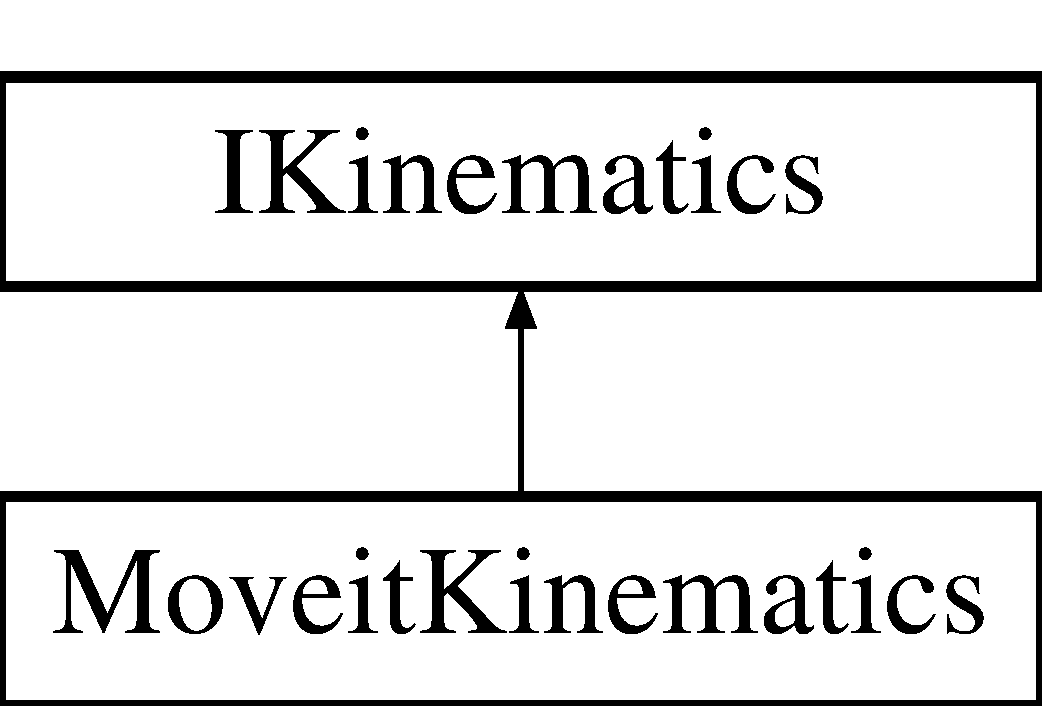
\includegraphics[height=2.000000cm]{classMoveitKinematics}
\end{center}
\end{figure}
\subsection*{Public Member Functions}
\begin{DoxyCompactItemize}
\item 
\hyperlink{classMoveitKinematics_aff96ca668755f869ba25a4a775e15eac}{Moveit\-Kinematics} (ros\-::\-Node\-Handle \&nh)
\item 
virtual std\-::vector$<$ double $>$ \hyperlink{classMoveitKinematics_a8f186684d000616a6ff805fa0f41151e}{Get\-Joint\-Values} ()
\begin{DoxyCompactList}\small\item\em Get\-Joint\-Values returns latest reading of end effector. \end{DoxyCompactList}\item 
virtual void \hyperlink{classMoveitKinematics_aee274ed4deddecb36191f8711c4b7c2e}{Set\-Joint\-Values} (std\-::vector$<$ double $>$ \hyperlink{classMoveitKinematics_a0ae2d3b65c1855ec6d6f094d1cd267f7}{joint\-\_\-values})
\begin{DoxyCompactList}\small\item\em Set\-Joint\-Values sets the latest joint values of the robot. \end{DoxyCompactList}\item 
virtual \hyperlink{namespaceRCS_aa07e45d8a50e30064283d2b38087f999}{R\-C\-S\-::\-Pose} \hyperlink{classMoveitKinematics_aef65c355097c1b8373f5bd60ef1b92f8}{F\-K} (std\-::vector$<$ double $>$ jv)
\begin{DoxyCompactList}\small\item\em F\-K performs the forward kinematics using the joint values of the robot provided. \end{DoxyCompactList}\item 
virtual std\-::vector$<$ double $>$ \hyperlink{classMoveitKinematics_a70fa6e222157b71b6bf8fa7ed33075cc}{I\-K} (\hyperlink{namespaceRCS_aa07e45d8a50e30064283d2b38087f999}{R\-C\-S\-::\-Pose} \&pose, std\-::vector$<$ double $>$ oldjoints)
\begin{DoxyCompactList}\small\item\em I\-K performs the inverse kinematics using the Cartesian pose provided. \end{DoxyCompactList}\item 
virtual size\-\_\-t \hyperlink{classMoveitKinematics_a256bfc139809c215c34112a38938a372}{All\-Pose\-To\-Joints} (\hyperlink{namespaceRCS_aa07e45d8a50e30064283d2b38087f999}{R\-C\-S\-::\-Pose} \&pose, std\-::vector$<$ std\-::vector$<$ double $>$ $>$ \&newjoints)
\begin{DoxyCompactList}\small\item\em All\-Pose\-To\-Joints solves the inverse kinematics to find all solutions using the Cartesian pose provided. \end{DoxyCompactList}\item 
virtual std\-::vector$<$ double $>$ \hyperlink{classMoveitKinematics_acd060eacf93c71b0cfb61bd5c93ceb77}{Nearest\-Joints} (std\-::vector$<$ double $>$ oldjoints, std\-::vector$<$ std\-::vector$<$ double $>$ $>$ \&newjoints)
\begin{DoxyCompactList}\small\item\em Nearest\-Joints finds the joint set that is closest to the old joints. \end{DoxyCompactList}\item 
virtual void \hyperlink{classMoveitKinematics_a3d0a3d9eadca26b5a24dd9904fee6e91}{Init} (std\-::string groupname, std\-::string eelinkname)
\begin{DoxyCompactList}\small\item\em Init is necessary for R\-O\-S to initialize it kinematics using robot model . \end{DoxyCompactList}\end{DoxyCompactItemize}
\subsection*{Public Attributes}
\begin{DoxyCompactItemize}
\item 
boost\-::shared\-\_\-ptr\\*
$<$ moveit\-::planning\-\_\-interface\-::\-Move\-Group $>$ \hyperlink{classMoveitKinematics_a3581661c4c9d14201a64a8143f51da3e}{group}
\item 
robot\-\_\-model\-::\-Robot\-Model\-Ptr \hyperlink{classMoveitKinematics_a69d28b2a76e5f5d90cdee38e0a3d5965}{kinematic\-\_\-model}
\item 
robot\-\_\-state\-::\-Robot\-State\-Ptr \hyperlink{classMoveitKinematics_ad59ff2cb08c79d9337b6852da2d4aadf}{kinematic\-\_\-state}
\item 
robot\-\_\-state\-::\-Joint\-Model\-Group $\ast$ \hyperlink{classMoveitKinematics_aa988eb59ddeb9f734d9911a5f464f082}{joint\-\_\-model\-\_\-group}
\item 
std\-::vector$<$ double $>$ \hyperlink{classMoveitKinematics_a0ae2d3b65c1855ec6d6f094d1cd267f7}{joint\-\_\-values}
\item 
std\-::vector$<$ std\-::string $>$ \hyperlink{classMoveitKinematics_ab9ccffd768a0d30944f22db09fbb9f72}{joint\-\_\-names}
\item 
std\-::string \hyperlink{classMoveitKinematics_afb7a90e3cda4da3b515a6e4cc19babe2}{\-\_\-groupname}
\item 
std\-::string \hyperlink{classMoveitKinematics_a5a97c1d7f715983995df78a442901c9e}{\-\_\-eelinkname}
\item 
ros\-::\-Node\-Handle \& \hyperlink{classMoveitKinematics_acea7424509f44c5f77f379f356a547c8}{\-\_\-nh}
\item 
bool \hyperlink{classMoveitKinematics_aa03e65371bb97fce4c98cbb46e53f423}{\-\_\-b\-Init}
\item 
boost\-::mutex \hyperlink{classMoveitKinematics_a94dd916f6d9a7074ebd00356975d51ea}{kinmutex}
\end{DoxyCompactItemize}


\subsection{Detailed Description}
The \hyperlink{classMoveitKinematics}{Moveit\-Kinematics} class instantiates the \hyperlink{classIKinematics}{I\-Kinematics} abstract class and fills in the pure virtual functions with Moveit kinematic methods. 

\subsection{Constructor \& Destructor Documentation}
\hypertarget{classMoveitKinematics_aff96ca668755f869ba25a4a775e15eac}{\index{Moveit\-Kinematics@{Moveit\-Kinematics}!Moveit\-Kinematics@{Moveit\-Kinematics}}
\index{Moveit\-Kinematics@{Moveit\-Kinematics}!MoveitKinematics@{Moveit\-Kinematics}}
\subsubsection[{Moveit\-Kinematics}]{\setlength{\rightskip}{0pt plus 5cm}Moveit\-Kinematics\-::\-Moveit\-Kinematics (
\begin{DoxyParamCaption}
\item[{ros\-::\-Node\-Handle \&}]{nh}
\end{DoxyParamCaption}
)}}\label{classMoveitKinematics_aff96ca668755f869ba25a4a775e15eac}


\subsection{Member Function Documentation}
\hypertarget{classMoveitKinematics_a256bfc139809c215c34112a38938a372}{\index{Moveit\-Kinematics@{Moveit\-Kinematics}!All\-Pose\-To\-Joints@{All\-Pose\-To\-Joints}}
\index{All\-Pose\-To\-Joints@{All\-Pose\-To\-Joints}!MoveitKinematics@{Moveit\-Kinematics}}
\subsubsection[{All\-Pose\-To\-Joints}]{\setlength{\rightskip}{0pt plus 5cm}virtual size\-\_\-t Moveit\-Kinematics\-::\-All\-Pose\-To\-Joints (
\begin{DoxyParamCaption}
\item[{{\bf R\-C\-S\-::\-Pose} \&}]{pose, }
\item[{std\-::vector$<$ std\-::vector$<$ double $>$ $>$ \&}]{newjoints}
\end{DoxyParamCaption}
)\hspace{0.3cm}{\ttfamily [inline]}, {\ttfamily [virtual]}}}\label{classMoveitKinematics_a256bfc139809c215c34112a38938a372}


All\-Pose\-To\-Joints solves the inverse kinematics to find all solutions using the Cartesian pose provided. 


\begin{DoxyParams}{Parameters}
{\em Cartesian} & robot pose of end effector. \\
\hline
{\em vector} & of double vectos to hold all the I\-K joint solutions. \\
\hline
\end{DoxyParams}
\begin{DoxyReturn}{Returns}
number of solutions found. 
\end{DoxyReturn}


Implements \hyperlink{classIKinematics_aeb53bb4b2a1e70a79d5d724e5eb82c10}{I\-Kinematics}.

\hypertarget{classMoveitKinematics_aef65c355097c1b8373f5bd60ef1b92f8}{\index{Moveit\-Kinematics@{Moveit\-Kinematics}!F\-K@{F\-K}}
\index{F\-K@{F\-K}!MoveitKinematics@{Moveit\-Kinematics}}
\subsubsection[{F\-K}]{\setlength{\rightskip}{0pt plus 5cm}{\bf R\-C\-S\-::\-Pose} Moveit\-Kinematics\-::\-F\-K (
\begin{DoxyParamCaption}
\item[{std\-::vector$<$ double $>$}]{jv}
\end{DoxyParamCaption}
)\hspace{0.3cm}{\ttfamily [virtual]}}}\label{classMoveitKinematics_aef65c355097c1b8373f5bd60ef1b92f8}


F\-K performs the forward kinematics using the joint values of the robot provided. 


\begin{DoxyParams}{Parameters}
{\em vector} & of all robot joint values in doubles. \\
\hline
\end{DoxyParams}
\begin{DoxyReturn}{Returns}
corresponding Cartesian robot pose of end effector. 
\end{DoxyReturn}


Implements \hyperlink{classIKinematics_abf765053ac39fac5b94ef99e80b17f1b}{I\-Kinematics}.

\hypertarget{classMoveitKinematics_a8f186684d000616a6ff805fa0f41151e}{\index{Moveit\-Kinematics@{Moveit\-Kinematics}!Get\-Joint\-Values@{Get\-Joint\-Values}}
\index{Get\-Joint\-Values@{Get\-Joint\-Values}!MoveitKinematics@{Moveit\-Kinematics}}
\subsubsection[{Get\-Joint\-Values}]{\setlength{\rightskip}{0pt plus 5cm}std\-::vector$<$ double $>$ Moveit\-Kinematics\-::\-Get\-Joint\-Values (
\begin{DoxyParamCaption}
{}
\end{DoxyParamCaption}
)\hspace{0.3cm}{\ttfamily [virtual]}}}\label{classMoveitKinematics_a8f186684d000616a6ff805fa0f41151e}


Get\-Joint\-Values returns latest reading of end effector. 

\begin{DoxyReturn}{Returns}
vector of joint values in doubles. 
\end{DoxyReturn}


Implements \hyperlink{classIKinematics_af41a85f8dc0cac9d94f982c7cf58b475}{I\-Kinematics}.

\hypertarget{classMoveitKinematics_a70fa6e222157b71b6bf8fa7ed33075cc}{\index{Moveit\-Kinematics@{Moveit\-Kinematics}!I\-K@{I\-K}}
\index{I\-K@{I\-K}!MoveitKinematics@{Moveit\-Kinematics}}
\subsubsection[{I\-K}]{\setlength{\rightskip}{0pt plus 5cm}std\-::vector$<$ double $>$ Moveit\-Kinematics\-::\-I\-K (
\begin{DoxyParamCaption}
\item[{{\bf R\-C\-S\-::\-Pose} \&}]{pose, }
\item[{std\-::vector$<$ double $>$}]{oldjoints}
\end{DoxyParamCaption}
)\hspace{0.3cm}{\ttfamily [virtual]}}}\label{classMoveitKinematics_a70fa6e222157b71b6bf8fa7ed33075cc}


I\-K performs the inverse kinematics using the Cartesian pose provided. 


\begin{DoxyParams}{Parameters}
{\em Cartesian} & robot pose of end effector. \\
\hline
{\em optional} & seed joint values to use as best guess for I\-K joint values. \\
\hline
\end{DoxyParams}
\begin{DoxyReturn}{Returns}
vector of all robot joint values in doubles. 
\end{DoxyReturn}


Implements \hyperlink{classIKinematics_ad0715c776a7eb325d2543bc34fa8114f}{I\-Kinematics}.

\hypertarget{classMoveitKinematics_a3d0a3d9eadca26b5a24dd9904fee6e91}{\index{Moveit\-Kinematics@{Moveit\-Kinematics}!Init@{Init}}
\index{Init@{Init}!MoveitKinematics@{Moveit\-Kinematics}}
\subsubsection[{Init}]{\setlength{\rightskip}{0pt plus 5cm}void Moveit\-Kinematics\-::\-Init (
\begin{DoxyParamCaption}
\item[{std\-::string}]{groupname, }
\item[{std\-::string}]{eelinkname}
\end{DoxyParamCaption}
)\hspace{0.3cm}{\ttfamily [virtual]}}}\label{classMoveitKinematics_a3d0a3d9eadca26b5a24dd9904fee6e91}


Init is necessary for R\-O\-S to initialize it kinematics using robot model . 


\begin{DoxyParams}{Parameters}
{\em groupname} & name of chained joints in robot model. \\
\hline
{\em eelinkname} & name of end effector joint in robot model. \\
\hline
\end{DoxyParams}


Reimplemented from \hyperlink{classIKinematics_a1407620d6cf7f26e61a64af42d570b8f}{I\-Kinematics}.

\hypertarget{classMoveitKinematics_acd060eacf93c71b0cfb61bd5c93ceb77}{\index{Moveit\-Kinematics@{Moveit\-Kinematics}!Nearest\-Joints@{Nearest\-Joints}}
\index{Nearest\-Joints@{Nearest\-Joints}!MoveitKinematics@{Moveit\-Kinematics}}
\subsubsection[{Nearest\-Joints}]{\setlength{\rightskip}{0pt plus 5cm}virtual std\-::vector$<$double$>$ Moveit\-Kinematics\-::\-Nearest\-Joints (
\begin{DoxyParamCaption}
\item[{std\-::vector$<$ double $>$}]{oldjoints, }
\item[{std\-::vector$<$ std\-::vector$<$ double $>$ $>$ \&}]{newjoints}
\end{DoxyParamCaption}
)\hspace{0.3cm}{\ttfamily [inline]}, {\ttfamily [virtual]}}}\label{classMoveitKinematics_acd060eacf93c71b0cfb61bd5c93ceb77}


Nearest\-Joints finds the joint set that is closest to the old joints. 


\begin{DoxyParams}{Parameters}
{\em old} & seed joint values to use as best guess for I\-K joint values. \\
\hline
{\em vector} & of double vectos that holds all the I\-K joint solutions. \\
\hline
\end{DoxyParams}
\begin{DoxyReturn}{Returns}
vector of doubles with closest set to seed joints. 
\end{DoxyReturn}


Implements \hyperlink{classIKinematics_ab74b70ed6ecc53adfc36505b8dd1fef4}{I\-Kinematics}.

\hypertarget{classMoveitKinematics_aee274ed4deddecb36191f8711c4b7c2e}{\index{Moveit\-Kinematics@{Moveit\-Kinematics}!Set\-Joint\-Values@{Set\-Joint\-Values}}
\index{Set\-Joint\-Values@{Set\-Joint\-Values}!MoveitKinematics@{Moveit\-Kinematics}}
\subsubsection[{Set\-Joint\-Values}]{\setlength{\rightskip}{0pt plus 5cm}void Moveit\-Kinematics\-::\-Set\-Joint\-Values (
\begin{DoxyParamCaption}
\item[{std\-::vector$<$ double $>$}]{joint\-\_\-values}
\end{DoxyParamCaption}
)\hspace{0.3cm}{\ttfamily [virtual]}}}\label{classMoveitKinematics_aee274ed4deddecb36191f8711c4b7c2e}


Set\-Joint\-Values sets the latest joint values of the robot. 


\begin{DoxyParams}{Parameters}
{\em vector} & of all robot joint values in doubles. \\
\hline
\end{DoxyParams}


Implements \hyperlink{classIKinematics_ad43b2185f06e20eb0bf9d5a94d4aec18}{I\-Kinematics}.



\subsection{Member Data Documentation}
\hypertarget{classMoveitKinematics_aa03e65371bb97fce4c98cbb46e53f423}{\index{Moveit\-Kinematics@{Moveit\-Kinematics}!\-\_\-b\-Init@{\-\_\-b\-Init}}
\index{\-\_\-b\-Init@{\-\_\-b\-Init}!MoveitKinematics@{Moveit\-Kinematics}}
\subsubsection[{\-\_\-b\-Init}]{\setlength{\rightskip}{0pt plus 5cm}bool Moveit\-Kinematics\-::\-\_\-b\-Init}}\label{classMoveitKinematics_aa03e65371bb97fce4c98cbb46e53f423}
\hypertarget{classMoveitKinematics_a5a97c1d7f715983995df78a442901c9e}{\index{Moveit\-Kinematics@{Moveit\-Kinematics}!\-\_\-eelinkname@{\-\_\-eelinkname}}
\index{\-\_\-eelinkname@{\-\_\-eelinkname}!MoveitKinematics@{Moveit\-Kinematics}}
\subsubsection[{\-\_\-eelinkname}]{\setlength{\rightskip}{0pt plus 5cm}std\-::string Moveit\-Kinematics\-::\-\_\-eelinkname}}\label{classMoveitKinematics_a5a97c1d7f715983995df78a442901c9e}
\hypertarget{classMoveitKinematics_afb7a90e3cda4da3b515a6e4cc19babe2}{\index{Moveit\-Kinematics@{Moveit\-Kinematics}!\-\_\-groupname@{\-\_\-groupname}}
\index{\-\_\-groupname@{\-\_\-groupname}!MoveitKinematics@{Moveit\-Kinematics}}
\subsubsection[{\-\_\-groupname}]{\setlength{\rightskip}{0pt plus 5cm}std\-::string Moveit\-Kinematics\-::\-\_\-groupname}}\label{classMoveitKinematics_afb7a90e3cda4da3b515a6e4cc19babe2}
\hypertarget{classMoveitKinematics_acea7424509f44c5f77f379f356a547c8}{\index{Moveit\-Kinematics@{Moveit\-Kinematics}!\-\_\-nh@{\-\_\-nh}}
\index{\-\_\-nh@{\-\_\-nh}!MoveitKinematics@{Moveit\-Kinematics}}
\subsubsection[{\-\_\-nh}]{\setlength{\rightskip}{0pt plus 5cm}ros\-::\-Node\-Handle\& Moveit\-Kinematics\-::\-\_\-nh}}\label{classMoveitKinematics_acea7424509f44c5f77f379f356a547c8}
\hypertarget{classMoveitKinematics_a3581661c4c9d14201a64a8143f51da3e}{\index{Moveit\-Kinematics@{Moveit\-Kinematics}!group@{group}}
\index{group@{group}!MoveitKinematics@{Moveit\-Kinematics}}
\subsubsection[{group}]{\setlength{\rightskip}{0pt plus 5cm}boost\-::shared\-\_\-ptr$<$moveit\-::planning\-\_\-interface\-::\-Move\-Group$>$ Moveit\-Kinematics\-::group}}\label{classMoveitKinematics_a3581661c4c9d14201a64a8143f51da3e}
\hypertarget{classMoveitKinematics_aa988eb59ddeb9f734d9911a5f464f082}{\index{Moveit\-Kinematics@{Moveit\-Kinematics}!joint\-\_\-model\-\_\-group@{joint\-\_\-model\-\_\-group}}
\index{joint\-\_\-model\-\_\-group@{joint\-\_\-model\-\_\-group}!MoveitKinematics@{Moveit\-Kinematics}}
\subsubsection[{joint\-\_\-model\-\_\-group}]{\setlength{\rightskip}{0pt plus 5cm}robot\-\_\-state\-::\-Joint\-Model\-Group$\ast$ Moveit\-Kinematics\-::joint\-\_\-model\-\_\-group}}\label{classMoveitKinematics_aa988eb59ddeb9f734d9911a5f464f082}
\hypertarget{classMoveitKinematics_ab9ccffd768a0d30944f22db09fbb9f72}{\index{Moveit\-Kinematics@{Moveit\-Kinematics}!joint\-\_\-names@{joint\-\_\-names}}
\index{joint\-\_\-names@{joint\-\_\-names}!MoveitKinematics@{Moveit\-Kinematics}}
\subsubsection[{joint\-\_\-names}]{\setlength{\rightskip}{0pt plus 5cm}std\-::vector$<$std\-::string$>$ Moveit\-Kinematics\-::joint\-\_\-names}}\label{classMoveitKinematics_ab9ccffd768a0d30944f22db09fbb9f72}
\hypertarget{classMoveitKinematics_a0ae2d3b65c1855ec6d6f094d1cd267f7}{\index{Moveit\-Kinematics@{Moveit\-Kinematics}!joint\-\_\-values@{joint\-\_\-values}}
\index{joint\-\_\-values@{joint\-\_\-values}!MoveitKinematics@{Moveit\-Kinematics}}
\subsubsection[{joint\-\_\-values}]{\setlength{\rightskip}{0pt plus 5cm}std\-::vector$<$double$>$ Moveit\-Kinematics\-::joint\-\_\-values}}\label{classMoveitKinematics_a0ae2d3b65c1855ec6d6f094d1cd267f7}
\hypertarget{classMoveitKinematics_a69d28b2a76e5f5d90cdee38e0a3d5965}{\index{Moveit\-Kinematics@{Moveit\-Kinematics}!kinematic\-\_\-model@{kinematic\-\_\-model}}
\index{kinematic\-\_\-model@{kinematic\-\_\-model}!MoveitKinematics@{Moveit\-Kinematics}}
\subsubsection[{kinematic\-\_\-model}]{\setlength{\rightskip}{0pt plus 5cm}robot\-\_\-model\-::\-Robot\-Model\-Ptr Moveit\-Kinematics\-::kinematic\-\_\-model}}\label{classMoveitKinematics_a69d28b2a76e5f5d90cdee38e0a3d5965}
\hypertarget{classMoveitKinematics_ad59ff2cb08c79d9337b6852da2d4aadf}{\index{Moveit\-Kinematics@{Moveit\-Kinematics}!kinematic\-\_\-state@{kinematic\-\_\-state}}
\index{kinematic\-\_\-state@{kinematic\-\_\-state}!MoveitKinematics@{Moveit\-Kinematics}}
\subsubsection[{kinematic\-\_\-state}]{\setlength{\rightskip}{0pt plus 5cm}robot\-\_\-state\-::\-Robot\-State\-Ptr Moveit\-Kinematics\-::kinematic\-\_\-state}}\label{classMoveitKinematics_ad59ff2cb08c79d9337b6852da2d4aadf}
\hypertarget{classMoveitKinematics_a94dd916f6d9a7074ebd00356975d51ea}{\index{Moveit\-Kinematics@{Moveit\-Kinematics}!kinmutex@{kinmutex}}
\index{kinmutex@{kinmutex}!MoveitKinematics@{Moveit\-Kinematics}}
\subsubsection[{kinmutex}]{\setlength{\rightskip}{0pt plus 5cm}boost\-::mutex Moveit\-Kinematics\-::kinmutex}}\label{classMoveitKinematics_a94dd916f6d9a7074ebd00356975d51ea}


The documentation for this class was generated from the following files\-:\begin{DoxyCompactItemize}
\item 
/home/michalos/catkin\-\_\-ws/src/nist\-\_\-fanuc/include/nist\-\_\-fanuc/\hyperlink{Kinematics_8h}{Kinematics.\-h}\item 
/home/michalos/catkin\-\_\-ws/src/nist\-\_\-fanuc/src/\hyperlink{Kinematics_8cpp}{Kinematics.\-cpp}\end{DoxyCompactItemize}

\hypertarget{classMoveitPlanning}{\section{Moveit\-Planning Class Reference}
\label{classMoveitPlanning}\index{Moveit\-Planning@{Moveit\-Planning}}
}


{\ttfamily \#include $<$moveit.\-h$>$}

\subsection*{Public Member Functions}
\begin{DoxyCompactItemize}
\item 
\hyperlink{classMoveitPlanning_a4138e1aed9641e0df587ec2b7e0663fe}{Moveit\-Planning} (ros\-::\-Node\-Handle \&nh)
\item 
\hyperlink{classMoveitPlanning_a0665e6d78bc4ee6c58c58ba1b43f6b7a}{$\sim$\-Moveit\-Planning} ()
\item 
std\-::vector$<$ \hyperlink{RCS_8h_aa4adb93a26caa4dacba9c9614e283245}{Joint\-State} $>$ \hyperlink{classMoveitPlanning_adcd57dfed95d3628cffbe5b88f0896cf}{Get\-Jts\-Plan} ()
\item 
bool \hyperlink{classMoveitPlanning_a37dd79bdbcb114884100bd68b5f107b7}{Plan} (\hyperlink{RCS_8h_aa4adb93a26caa4dacba9c9614e283245}{Joint\-State} curjoints, \hyperlink{RCS_8h_aa4adb93a26caa4dacba9c9614e283245}{Joint\-State} goaljoints)
\item 
bool \hyperlink{classMoveitPlanning_ab83293f9a377f8539c949ffdd5c89e0a}{Plan} (urdf\-::\-Pose \&curpose, urdf\-::\-Pose \&goalpose)
\item 
bool \hyperlink{classMoveitPlanning_a0d645edc1964fd98600798f4c7474a16}{Plan} (urdf\-::\-Pose \&pose)
\item 
bool \hyperlink{classMoveitPlanning_a10f7770fcaa229cdffd2f63215bed37b}{Plan} (std\-::vector$<$ urdf\-::\-Pose $>$ \&waypoints)
\item 
bool \hyperlink{classMoveitPlanning_a21c7727e0906a6ed2e24a31165ed3ba6}{Plan} (\hyperlink{RCS_8h_aa4adb93a26caa4dacba9c9614e283245}{Joint\-State} joints)
\item 
bool \hyperlink{classMoveitPlanning_a535856f4f406cb7d2f89c0bd03618109}{Plan} (Eigen\-::\-Affine3d \&pose)
\item 
bool \hyperlink{classMoveitPlanning_ac0e53ee15cf0ac2f605422534963d78e}{Plan} (geometry\-\_\-msgs\-::\-Pose \&pose)
\item 
urdf\-::\-Pose \hyperlink{classMoveitPlanning_ab5304af5d89d46daafa10a5b7698a006}{Get\-Current\-Pose} ()
\item 
std\-::vector$<$ double $>$ \hyperlink{classMoveitPlanning_a4ad173a662340daf91ab2ddde44e0946}{Get\-Joint\-Values} ()
\item 
urdf\-::\-Pose \hyperlink{classMoveitPlanning_a0417e420f1c97c887e5e4b70ebebdb57}{Forward\-Kinematics} ()
\item 
std\-::vector$<$ double $>$ \hyperlink{classMoveitPlanning_a8e98e6c54141fc0a3ef92cfcef7bcfa5}{Set\-Random\-Joints} ()
\item 
void \hyperlink{classMoveitPlanning_abe8bbc034b09c7935ee2a54d557fb5c8}{Display\-Plan} ()
\item 
void \hyperlink{classMoveitPlanning_a99ae8ab8c7047f95d114701f1f3f2a49}{Save\-Plan} ()
\item 
boost\-::shared\-\_\-ptr\\*
$<$ moveit\-::planning\-\_\-interface\-::\-Move\-Group $>$ \hyperlink{classMoveitPlanning_ae8754bf6b519a2fc6ada11a44989479b}{Get\-Group} ()
\item 
std\-::vector$<$ std\-::string $>$ \hyperlink{classMoveitPlanning_a26149b824c249979b28fcb46d4909668}{Get\-Joint\-Names} ()
\end{DoxyCompactItemize}
\subsection*{Public Attributes}
\begin{DoxyCompactItemize}
\item 
moveit\-::planning\-\_\-interface\-::\-Move\-Group\-::\-Plan \hyperlink{classMoveitPlanning_a981942759c10b3127a9d8d80ae54ef44}{my\-\_\-plan}
\item 
boost\-::shared\-\_\-ptr\\*
$<$ moveit\-::planning\-\_\-interface\-::\-Move\-Group $>$ \hyperlink{classMoveitPlanning_a8c2fe5775408e0e3afe6288f9b9facd5}{group}
\item 
robot\-\_\-model\-::\-Robot\-Model\-Ptr \hyperlink{classMoveitPlanning_a9311edd62f690d6fb5398e62df2df18c}{kinematic\-\_\-model}
\item 
robot\-\_\-state\-::\-Robot\-State\-Ptr \hyperlink{classMoveitPlanning_af7d64860fac3ae411904770755904345}{kinematic\-\_\-state}
\item 
robot\-\_\-state\-::\-Joint\-Model\-Group $\ast$ \hyperlink{classMoveitPlanning_a1e4e53d7560c0148712e7cc00b314085}{joint\-\_\-model\-\_\-group}
\item 
std\-::string \hyperlink{classMoveitPlanning_a56cf116dfd39c4ba4fb16df4b70c8a29}{\-\_\-groupname}
\item 
std\-::vector$<$ std\-::string $>$ \hyperlink{classMoveitPlanning_a36a6b85e1318172afbcce875a73cea10}{joint\-\_\-names}
\item 
bool \hyperlink{classMoveitPlanning_a64c359d7383623d1dc1976060a5a8e73}{\-\_\-b\-Inited}
\item 
ros\-::\-Publisher \hyperlink{classMoveitPlanning_a51be3d19d403e4872374062888171a22}{display\-\_\-publisher}
\item 
std\-::vector$<$ \hyperlink{RCS_8h_aa4adb93a26caa4dacba9c9614e283245}{Joint\-State} $>$ \hyperlink{classMoveitPlanning_ae0a57c1497f666564f307e1f53f2b974}{plannedjts}
\end{DoxyCompactItemize}


\subsection{Constructor \& Destructor Documentation}
\hypertarget{classMoveitPlanning_a4138e1aed9641e0df587ec2b7e0663fe}{\index{Moveit\-Planning@{Moveit\-Planning}!Moveit\-Planning@{Moveit\-Planning}}
\index{Moveit\-Planning@{Moveit\-Planning}!MoveitPlanning@{Moveit\-Planning}}
\subsubsection[{Moveit\-Planning}]{\setlength{\rightskip}{0pt plus 5cm}Moveit\-Planning\-::\-Moveit\-Planning (
\begin{DoxyParamCaption}
\item[{ros\-::\-Node\-Handle \&}]{nh}
\end{DoxyParamCaption}
)}}\label{classMoveitPlanning_a4138e1aed9641e0df587ec2b7e0663fe}
\hypertarget{classMoveitPlanning_a0665e6d78bc4ee6c58c58ba1b43f6b7a}{\index{Moveit\-Planning@{Moveit\-Planning}!$\sim$\-Moveit\-Planning@{$\sim$\-Moveit\-Planning}}
\index{$\sim$\-Moveit\-Planning@{$\sim$\-Moveit\-Planning}!MoveitPlanning@{Moveit\-Planning}}
\subsubsection[{$\sim$\-Moveit\-Planning}]{\setlength{\rightskip}{0pt plus 5cm}Moveit\-Planning\-::$\sim$\-Moveit\-Planning (
\begin{DoxyParamCaption}
{}
\end{DoxyParamCaption}
)}}\label{classMoveitPlanning_a0665e6d78bc4ee6c58c58ba1b43f6b7a}


\subsection{Member Function Documentation}
\hypertarget{classMoveitPlanning_abe8bbc034b09c7935ee2a54d557fb5c8}{\index{Moveit\-Planning@{Moveit\-Planning}!Display\-Plan@{Display\-Plan}}
\index{Display\-Plan@{Display\-Plan}!MoveitPlanning@{Moveit\-Planning}}
\subsubsection[{Display\-Plan}]{\setlength{\rightskip}{0pt plus 5cm}void Moveit\-Planning\-::\-Display\-Plan (
\begin{DoxyParamCaption}
{}
\end{DoxyParamCaption}
)}}\label{classMoveitPlanning_abe8bbc034b09c7935ee2a54d557fb5c8}
\hypertarget{classMoveitPlanning_a0417e420f1c97c887e5e4b70ebebdb57}{\index{Moveit\-Planning@{Moveit\-Planning}!Forward\-Kinematics@{Forward\-Kinematics}}
\index{Forward\-Kinematics@{Forward\-Kinematics}!MoveitPlanning@{Moveit\-Planning}}
\subsubsection[{Forward\-Kinematics}]{\setlength{\rightskip}{0pt plus 5cm}urdf\-::\-Pose Moveit\-Planning\-::\-Forward\-Kinematics (
\begin{DoxyParamCaption}
{}
\end{DoxyParamCaption}
)}}\label{classMoveitPlanning_a0417e420f1c97c887e5e4b70ebebdb57}
\hypertarget{classMoveitPlanning_ab5304af5d89d46daafa10a5b7698a006}{\index{Moveit\-Planning@{Moveit\-Planning}!Get\-Current\-Pose@{Get\-Current\-Pose}}
\index{Get\-Current\-Pose@{Get\-Current\-Pose}!MoveitPlanning@{Moveit\-Planning}}
\subsubsection[{Get\-Current\-Pose}]{\setlength{\rightskip}{0pt plus 5cm}urdf\-::\-Pose Moveit\-Planning\-::\-Get\-Current\-Pose (
\begin{DoxyParamCaption}
{}
\end{DoxyParamCaption}
)}}\label{classMoveitPlanning_ab5304af5d89d46daafa10a5b7698a006}
\hypertarget{classMoveitPlanning_ae8754bf6b519a2fc6ada11a44989479b}{\index{Moveit\-Planning@{Moveit\-Planning}!Get\-Group@{Get\-Group}}
\index{Get\-Group@{Get\-Group}!MoveitPlanning@{Moveit\-Planning}}
\subsubsection[{Get\-Group}]{\setlength{\rightskip}{0pt plus 5cm}boost\-::shared\-\_\-ptr$<$moveit\-::planning\-\_\-interface\-::\-Move\-Group$>$ Moveit\-Planning\-::\-Get\-Group (
\begin{DoxyParamCaption}
{}
\end{DoxyParamCaption}
)\hspace{0.3cm}{\ttfamily [inline]}}}\label{classMoveitPlanning_ae8754bf6b519a2fc6ada11a44989479b}
\hypertarget{classMoveitPlanning_a26149b824c249979b28fcb46d4909668}{\index{Moveit\-Planning@{Moveit\-Planning}!Get\-Joint\-Names@{Get\-Joint\-Names}}
\index{Get\-Joint\-Names@{Get\-Joint\-Names}!MoveitPlanning@{Moveit\-Planning}}
\subsubsection[{Get\-Joint\-Names}]{\setlength{\rightskip}{0pt plus 5cm}std\-::vector$<$std\-::string$>$ Moveit\-Planning\-::\-Get\-Joint\-Names (
\begin{DoxyParamCaption}
{}
\end{DoxyParamCaption}
)\hspace{0.3cm}{\ttfamily [inline]}}}\label{classMoveitPlanning_a26149b824c249979b28fcb46d4909668}
\hypertarget{classMoveitPlanning_a4ad173a662340daf91ab2ddde44e0946}{\index{Moveit\-Planning@{Moveit\-Planning}!Get\-Joint\-Values@{Get\-Joint\-Values}}
\index{Get\-Joint\-Values@{Get\-Joint\-Values}!MoveitPlanning@{Moveit\-Planning}}
\subsubsection[{Get\-Joint\-Values}]{\setlength{\rightskip}{0pt plus 5cm}std\-::vector$<$ double $>$ Moveit\-Planning\-::\-Get\-Joint\-Values (
\begin{DoxyParamCaption}
{}
\end{DoxyParamCaption}
)}}\label{classMoveitPlanning_a4ad173a662340daf91ab2ddde44e0946}
\hypertarget{classMoveitPlanning_adcd57dfed95d3628cffbe5b88f0896cf}{\index{Moveit\-Planning@{Moveit\-Planning}!Get\-Jts\-Plan@{Get\-Jts\-Plan}}
\index{Get\-Jts\-Plan@{Get\-Jts\-Plan}!MoveitPlanning@{Moveit\-Planning}}
\subsubsection[{Get\-Jts\-Plan}]{\setlength{\rightskip}{0pt plus 5cm}std\-::vector$<$ {\bf Joint\-State} $>$ Moveit\-Planning\-::\-Get\-Jts\-Plan (
\begin{DoxyParamCaption}
{}
\end{DoxyParamCaption}
)}}\label{classMoveitPlanning_adcd57dfed95d3628cffbe5b88f0896cf}
\hypertarget{classMoveitPlanning_a37dd79bdbcb114884100bd68b5f107b7}{\index{Moveit\-Planning@{Moveit\-Planning}!Plan@{Plan}}
\index{Plan@{Plan}!MoveitPlanning@{Moveit\-Planning}}
\subsubsection[{Plan}]{\setlength{\rightskip}{0pt plus 5cm}bool Moveit\-Planning\-::\-Plan (
\begin{DoxyParamCaption}
\item[{{\bf Joint\-State}}]{curjoints, }
\item[{{\bf Joint\-State}}]{goaljoints}
\end{DoxyParamCaption}
)}}\label{classMoveitPlanning_a37dd79bdbcb114884100bd68b5f107b7}
\hypertarget{classMoveitPlanning_ab83293f9a377f8539c949ffdd5c89e0a}{\index{Moveit\-Planning@{Moveit\-Planning}!Plan@{Plan}}
\index{Plan@{Plan}!MoveitPlanning@{Moveit\-Planning}}
\subsubsection[{Plan}]{\setlength{\rightskip}{0pt plus 5cm}bool Moveit\-Planning\-::\-Plan (
\begin{DoxyParamCaption}
\item[{urdf\-::\-Pose \&}]{curpose, }
\item[{urdf\-::\-Pose \&}]{goalpose}
\end{DoxyParamCaption}
)}}\label{classMoveitPlanning_ab83293f9a377f8539c949ffdd5c89e0a}
\hypertarget{classMoveitPlanning_a0d645edc1964fd98600798f4c7474a16}{\index{Moveit\-Planning@{Moveit\-Planning}!Plan@{Plan}}
\index{Plan@{Plan}!MoveitPlanning@{Moveit\-Planning}}
\subsubsection[{Plan}]{\setlength{\rightskip}{0pt plus 5cm}bool Moveit\-Planning\-::\-Plan (
\begin{DoxyParamCaption}
\item[{urdf\-::\-Pose \&}]{pose}
\end{DoxyParamCaption}
)}}\label{classMoveitPlanning_a0d645edc1964fd98600798f4c7474a16}
\hypertarget{classMoveitPlanning_a10f7770fcaa229cdffd2f63215bed37b}{\index{Moveit\-Planning@{Moveit\-Planning}!Plan@{Plan}}
\index{Plan@{Plan}!MoveitPlanning@{Moveit\-Planning}}
\subsubsection[{Plan}]{\setlength{\rightskip}{0pt plus 5cm}bool Moveit\-Planning\-::\-Plan (
\begin{DoxyParamCaption}
\item[{std\-::vector$<$ urdf\-::\-Pose $>$ \&}]{waypoints}
\end{DoxyParamCaption}
)}}\label{classMoveitPlanning_a10f7770fcaa229cdffd2f63215bed37b}
\hypertarget{classMoveitPlanning_a21c7727e0906a6ed2e24a31165ed3ba6}{\index{Moveit\-Planning@{Moveit\-Planning}!Plan@{Plan}}
\index{Plan@{Plan}!MoveitPlanning@{Moveit\-Planning}}
\subsubsection[{Plan}]{\setlength{\rightskip}{0pt plus 5cm}bool Moveit\-Planning\-::\-Plan (
\begin{DoxyParamCaption}
\item[{{\bf Joint\-State}}]{joints}
\end{DoxyParamCaption}
)}}\label{classMoveitPlanning_a21c7727e0906a6ed2e24a31165ed3ba6}
\hypertarget{classMoveitPlanning_a535856f4f406cb7d2f89c0bd03618109}{\index{Moveit\-Planning@{Moveit\-Planning}!Plan@{Plan}}
\index{Plan@{Plan}!MoveitPlanning@{Moveit\-Planning}}
\subsubsection[{Plan}]{\setlength{\rightskip}{0pt plus 5cm}bool Moveit\-Planning\-::\-Plan (
\begin{DoxyParamCaption}
\item[{Eigen\-::\-Affine3d \&}]{pose}
\end{DoxyParamCaption}
)}}\label{classMoveitPlanning_a535856f4f406cb7d2f89c0bd03618109}
\hypertarget{classMoveitPlanning_ac0e53ee15cf0ac2f605422534963d78e}{\index{Moveit\-Planning@{Moveit\-Planning}!Plan@{Plan}}
\index{Plan@{Plan}!MoveitPlanning@{Moveit\-Planning}}
\subsubsection[{Plan}]{\setlength{\rightskip}{0pt plus 5cm}bool Moveit\-Planning\-::\-Plan (
\begin{DoxyParamCaption}
\item[{geometry\-\_\-msgs\-::\-Pose \&}]{pose}
\end{DoxyParamCaption}
)}}\label{classMoveitPlanning_ac0e53ee15cf0ac2f605422534963d78e}
\hypertarget{classMoveitPlanning_a99ae8ab8c7047f95d114701f1f3f2a49}{\index{Moveit\-Planning@{Moveit\-Planning}!Save\-Plan@{Save\-Plan}}
\index{Save\-Plan@{Save\-Plan}!MoveitPlanning@{Moveit\-Planning}}
\subsubsection[{Save\-Plan}]{\setlength{\rightskip}{0pt plus 5cm}void Moveit\-Planning\-::\-Save\-Plan (
\begin{DoxyParamCaption}
{}
\end{DoxyParamCaption}
)}}\label{classMoveitPlanning_a99ae8ab8c7047f95d114701f1f3f2a49}
\hypertarget{classMoveitPlanning_a8e98e6c54141fc0a3ef92cfcef7bcfa5}{\index{Moveit\-Planning@{Moveit\-Planning}!Set\-Random\-Joints@{Set\-Random\-Joints}}
\index{Set\-Random\-Joints@{Set\-Random\-Joints}!MoveitPlanning@{Moveit\-Planning}}
\subsubsection[{Set\-Random\-Joints}]{\setlength{\rightskip}{0pt plus 5cm}std\-::vector$<$ double $>$ Moveit\-Planning\-::\-Set\-Random\-Joints (
\begin{DoxyParamCaption}
{}
\end{DoxyParamCaption}
)}}\label{classMoveitPlanning_a8e98e6c54141fc0a3ef92cfcef7bcfa5}


\subsection{Member Data Documentation}
\hypertarget{classMoveitPlanning_a64c359d7383623d1dc1976060a5a8e73}{\index{Moveit\-Planning@{Moveit\-Planning}!\-\_\-b\-Inited@{\-\_\-b\-Inited}}
\index{\-\_\-b\-Inited@{\-\_\-b\-Inited}!MoveitPlanning@{Moveit\-Planning}}
\subsubsection[{\-\_\-b\-Inited}]{\setlength{\rightskip}{0pt plus 5cm}bool Moveit\-Planning\-::\-\_\-b\-Inited}}\label{classMoveitPlanning_a64c359d7383623d1dc1976060a5a8e73}
\hypertarget{classMoveitPlanning_a56cf116dfd39c4ba4fb16df4b70c8a29}{\index{Moveit\-Planning@{Moveit\-Planning}!\-\_\-groupname@{\-\_\-groupname}}
\index{\-\_\-groupname@{\-\_\-groupname}!MoveitPlanning@{Moveit\-Planning}}
\subsubsection[{\-\_\-groupname}]{\setlength{\rightskip}{0pt plus 5cm}std\-::string Moveit\-Planning\-::\-\_\-groupname}}\label{classMoveitPlanning_a56cf116dfd39c4ba4fb16df4b70c8a29}
\hypertarget{classMoveitPlanning_a51be3d19d403e4872374062888171a22}{\index{Moveit\-Planning@{Moveit\-Planning}!display\-\_\-publisher@{display\-\_\-publisher}}
\index{display\-\_\-publisher@{display\-\_\-publisher}!MoveitPlanning@{Moveit\-Planning}}
\subsubsection[{display\-\_\-publisher}]{\setlength{\rightskip}{0pt plus 5cm}ros\-::\-Publisher Moveit\-Planning\-::display\-\_\-publisher}}\label{classMoveitPlanning_a51be3d19d403e4872374062888171a22}
\hypertarget{classMoveitPlanning_a8c2fe5775408e0e3afe6288f9b9facd5}{\index{Moveit\-Planning@{Moveit\-Planning}!group@{group}}
\index{group@{group}!MoveitPlanning@{Moveit\-Planning}}
\subsubsection[{group}]{\setlength{\rightskip}{0pt plus 5cm}boost\-::shared\-\_\-ptr$<$moveit\-::planning\-\_\-interface\-::\-Move\-Group$>$ Moveit\-Planning\-::group}}\label{classMoveitPlanning_a8c2fe5775408e0e3afe6288f9b9facd5}
\hypertarget{classMoveitPlanning_a1e4e53d7560c0148712e7cc00b314085}{\index{Moveit\-Planning@{Moveit\-Planning}!joint\-\_\-model\-\_\-group@{joint\-\_\-model\-\_\-group}}
\index{joint\-\_\-model\-\_\-group@{joint\-\_\-model\-\_\-group}!MoveitPlanning@{Moveit\-Planning}}
\subsubsection[{joint\-\_\-model\-\_\-group}]{\setlength{\rightskip}{0pt plus 5cm}robot\-\_\-state\-::\-Joint\-Model\-Group$\ast$ Moveit\-Planning\-::joint\-\_\-model\-\_\-group}}\label{classMoveitPlanning_a1e4e53d7560c0148712e7cc00b314085}
\hypertarget{classMoveitPlanning_a36a6b85e1318172afbcce875a73cea10}{\index{Moveit\-Planning@{Moveit\-Planning}!joint\-\_\-names@{joint\-\_\-names}}
\index{joint\-\_\-names@{joint\-\_\-names}!MoveitPlanning@{Moveit\-Planning}}
\subsubsection[{joint\-\_\-names}]{\setlength{\rightskip}{0pt plus 5cm}std\-::vector$<$std\-::string$>$ Moveit\-Planning\-::joint\-\_\-names}}\label{classMoveitPlanning_a36a6b85e1318172afbcce875a73cea10}
\hypertarget{classMoveitPlanning_a9311edd62f690d6fb5398e62df2df18c}{\index{Moveit\-Planning@{Moveit\-Planning}!kinematic\-\_\-model@{kinematic\-\_\-model}}
\index{kinematic\-\_\-model@{kinematic\-\_\-model}!MoveitPlanning@{Moveit\-Planning}}
\subsubsection[{kinematic\-\_\-model}]{\setlength{\rightskip}{0pt plus 5cm}robot\-\_\-model\-::\-Robot\-Model\-Ptr Moveit\-Planning\-::kinematic\-\_\-model}}\label{classMoveitPlanning_a9311edd62f690d6fb5398e62df2df18c}
\hypertarget{classMoveitPlanning_af7d64860fac3ae411904770755904345}{\index{Moveit\-Planning@{Moveit\-Planning}!kinematic\-\_\-state@{kinematic\-\_\-state}}
\index{kinematic\-\_\-state@{kinematic\-\_\-state}!MoveitPlanning@{Moveit\-Planning}}
\subsubsection[{kinematic\-\_\-state}]{\setlength{\rightskip}{0pt plus 5cm}robot\-\_\-state\-::\-Robot\-State\-Ptr Moveit\-Planning\-::kinematic\-\_\-state}}\label{classMoveitPlanning_af7d64860fac3ae411904770755904345}
\hypertarget{classMoveitPlanning_a981942759c10b3127a9d8d80ae54ef44}{\index{Moveit\-Planning@{Moveit\-Planning}!my\-\_\-plan@{my\-\_\-plan}}
\index{my\-\_\-plan@{my\-\_\-plan}!MoveitPlanning@{Moveit\-Planning}}
\subsubsection[{my\-\_\-plan}]{\setlength{\rightskip}{0pt plus 5cm}moveit\-::planning\-\_\-interface\-::\-Move\-Group\-::\-Plan Moveit\-Planning\-::my\-\_\-plan}}\label{classMoveitPlanning_a981942759c10b3127a9d8d80ae54ef44}
\hypertarget{classMoveitPlanning_ae0a57c1497f666564f307e1f53f2b974}{\index{Moveit\-Planning@{Moveit\-Planning}!plannedjts@{plannedjts}}
\index{plannedjts@{plannedjts}!MoveitPlanning@{Moveit\-Planning}}
\subsubsection[{plannedjts}]{\setlength{\rightskip}{0pt plus 5cm}std\-::vector$<${\bf Joint\-State}$>$ Moveit\-Planning\-::plannedjts}}\label{classMoveitPlanning_ae0a57c1497f666564f307e1f53f2b974}


The documentation for this class was generated from the following files\-:\begin{DoxyCompactItemize}
\item 
/home/michalos/catkin\-\_\-ws/src/nist\-\_\-fanuc/include/nist\-\_\-fanuc/\hyperlink{moveit_8h}{moveit.\-h}\item 
/home/michalos/catkin\-\_\-ws/src/nist\-\_\-fanuc/src/\hyperlink{moveit_8cpp}{moveit.\-cpp}\end{DoxyCompactItemize}

\hypertarget{classRCSInterpreter}{\section{R\-C\-S\-Interpreter Class Reference}
\label{classRCSInterpreter}\index{R\-C\-S\-Interpreter@{R\-C\-S\-Interpreter}}
}


\hyperlink{classRCSInterpreter}{R\-C\-S\-Interpreter} parses a \hyperlink{namespaceRCS}{R\-C\-S} command and generates robot motion commands.  




{\ttfamily \#include $<$R\-C\-S\-Interpreter.\-h$>$}

\subsection*{Public Member Functions}
\begin{DoxyCompactItemize}
\item 
\hyperlink{classRCSInterpreter_abf39be78f8107db4844c33434fe33caf}{R\-C\-S\-Interpreter} (\hyperlink{Kinematics_8h_aa720b9842c846588baf215581fb9f902}{I\-Kinematics\-Shared\-Ptr} k=N\-U\-L\-L)
\begin{DoxyCompactList}\small\item\em \hyperlink{classRCSInterpreter}{R\-C\-S\-Interpreter} constructor that optionally accepts pointer to kinematic instance. \end{DoxyCompactList}\item 
\hyperlink{classRCSInterpreter_a540468718197e24d7c20cc1f43696715}{$\sim$\-R\-C\-S\-Interpreter} (void)
\item 
int \hyperlink{classRCSInterpreter_a7f7cee6a3606a2b3f22ca3f802a1fc39}{Parse\-Command} (\hyperlink{structRCS_1_1CanonCmd}{R\-C\-S\-::\-Canon\-Cmd} cmd)
\begin{DoxyCompactList}\small\item\em Parse\-Command parses a \hyperlink{namespaceRCS}{R\-C\-S} command and queues robot motion commands. \end{DoxyCompactList}\end{DoxyCompactItemize}
\subsection*{Public Attributes}
\begin{DoxyCompactItemize}
\item 
\hyperlink{Kinematics_8h_aa720b9842c846588baf215581fb9f902}{I\-Kinematics\-Shared\-Ptr} \hyperlink{classRCSInterpreter_a0a78e67ba785253bf3de6877294da699}{\-\_\-kinematics}
\item 
\hyperlink{demo_8cpp_a2a09344c15175b0b6ea4da8bbffa8106}{Trajectory\-Vec} \hyperlink{classRCSInterpreter_a7b71ecaad68a14cc341d98d463e6f5b5}{results}
\item 
std\-::vector$<$ double $>$ \hyperlink{classRCSInterpreter_a2437a1768cfa972b39ff56c8f16ff3c1}{times}
\item 
\hyperlink{classIRate}{I\-Rate} \hyperlink{classRCSInterpreter_a11b1a673682a9d0451877d3b5c3e0e3e}{rates}
\item 
\hyperlink{classMotionControl}{Motion\-Control} \hyperlink{classRCSInterpreter_ae59648ec8d61ea6957bbd320f2a4665a}{motioncontrol}
\end{DoxyCompactItemize}
\subsection*{Protected Member Functions}
\begin{DoxyCompactItemize}
\item 
void \hyperlink{classRCSInterpreter_af33d7a81522ff6de4f7e56a20520c4de}{Add\-Joint\-Commands} (std\-::vector$<$ \hyperlink{RCS_8h_aa4adb93a26caa4dacba9c9614e283245}{Joint\-State} $>$ gotojoints)
\begin{DoxyCompactList}\small\item\em Add\-Joint\-Commands accepts vector of joint trajectories and adds to robot motion queue. \end{DoxyCompactList}\item 
std\-::vector$<$ \hyperlink{RCS_8h_aa4adb93a26caa4dacba9c9614e283245}{Joint\-State} $>$ \hyperlink{classRCSInterpreter_ad5393d870957f985f307a9aadd41231c}{Plan\-Cartesian\-Motion} (std\-::vector$<$ urdf\-::\-Pose $>$ poses)
\begin{DoxyCompactList}\small\item\em Plan\-Cartesian\-Motion accepts vector of poses and generates a vector of joint trajectories. Can use a couple of planning algorithms to generate trajectory. \end{DoxyCompactList}\end{DoxyCompactItemize}


\subsection{Detailed Description}
\hyperlink{classRCSInterpreter}{R\-C\-S\-Interpreter} parses a \hyperlink{namespaceRCS}{R\-C\-S} command and generates robot motion commands. 

\subsection{Constructor \& Destructor Documentation}
\hypertarget{classRCSInterpreter_abf39be78f8107db4844c33434fe33caf}{\index{R\-C\-S\-Interpreter@{R\-C\-S\-Interpreter}!R\-C\-S\-Interpreter@{R\-C\-S\-Interpreter}}
\index{R\-C\-S\-Interpreter@{R\-C\-S\-Interpreter}!RCSInterpreter@{R\-C\-S\-Interpreter}}
\subsubsection[{R\-C\-S\-Interpreter}]{\setlength{\rightskip}{0pt plus 5cm}R\-C\-S\-Interpreter\-::\-R\-C\-S\-Interpreter (
\begin{DoxyParamCaption}
\item[{{\bf I\-Kinematics\-Shared\-Ptr}}]{k = {\ttfamily NULL}}
\end{DoxyParamCaption}
)}}\label{classRCSInterpreter_abf39be78f8107db4844c33434fe33caf}


\hyperlink{classRCSInterpreter}{R\-C\-S\-Interpreter} constructor that optionally accepts pointer to kinematic instance. 


\begin{DoxyParams}{Parameters}
{\em k} & is the kinematics pointer \\
\hline
\end{DoxyParams}
\hypertarget{classRCSInterpreter_a540468718197e24d7c20cc1f43696715}{\index{R\-C\-S\-Interpreter@{R\-C\-S\-Interpreter}!$\sim$\-R\-C\-S\-Interpreter@{$\sim$\-R\-C\-S\-Interpreter}}
\index{$\sim$\-R\-C\-S\-Interpreter@{$\sim$\-R\-C\-S\-Interpreter}!RCSInterpreter@{R\-C\-S\-Interpreter}}
\subsubsection[{$\sim$\-R\-C\-S\-Interpreter}]{\setlength{\rightskip}{0pt plus 5cm}R\-C\-S\-Interpreter\-::$\sim$\-R\-C\-S\-Interpreter (
\begin{DoxyParamCaption}
\item[{void}]{}
\end{DoxyParamCaption}
)}}\label{classRCSInterpreter_a540468718197e24d7c20cc1f43696715}


\subsection{Member Function Documentation}
\hypertarget{classRCSInterpreter_af33d7a81522ff6de4f7e56a20520c4de}{\index{R\-C\-S\-Interpreter@{R\-C\-S\-Interpreter}!Add\-Joint\-Commands@{Add\-Joint\-Commands}}
\index{Add\-Joint\-Commands@{Add\-Joint\-Commands}!RCSInterpreter@{R\-C\-S\-Interpreter}}
\subsubsection[{Add\-Joint\-Commands}]{\setlength{\rightskip}{0pt plus 5cm}void R\-C\-S\-Interpreter\-::\-Add\-Joint\-Commands (
\begin{DoxyParamCaption}
\item[{std\-::vector$<$ {\bf Joint\-State} $>$}]{gotojoints}
\end{DoxyParamCaption}
)\hspace{0.3cm}{\ttfamily [protected]}}}\label{classRCSInterpreter_af33d7a81522ff6de4f7e56a20520c4de}


Add\-Joint\-Commands accepts vector of joint trajectories and adds to robot motion queue. 


\begin{DoxyParams}{Parameters}
{\em gotojoints} & is the vector of joint states describing the motion. \\
\hline
\end{DoxyParams}
\hypertarget{classRCSInterpreter_a7f7cee6a3606a2b3f22ca3f802a1fc39}{\index{R\-C\-S\-Interpreter@{R\-C\-S\-Interpreter}!Parse\-Command@{Parse\-Command}}
\index{Parse\-Command@{Parse\-Command}!RCSInterpreter@{R\-C\-S\-Interpreter}}
\subsubsection[{Parse\-Command}]{\setlength{\rightskip}{0pt plus 5cm}int R\-C\-S\-Interpreter\-::\-Parse\-Command (
\begin{DoxyParamCaption}
\item[{{\bf R\-C\-S\-::\-Canon\-Cmd}}]{cmd}
\end{DoxyParamCaption}
)}}\label{classRCSInterpreter_a7f7cee6a3606a2b3f22ca3f802a1fc39}


Parse\-Command parses a \hyperlink{namespaceRCS}{R\-C\-S} command and queues robot motion commands. 


\begin{DoxyParams}{Parameters}
{\em cmd} & is the command to interpret \\
\hline
\end{DoxyParams}
\hypertarget{classRCSInterpreter_ad5393d870957f985f307a9aadd41231c}{\index{R\-C\-S\-Interpreter@{R\-C\-S\-Interpreter}!Plan\-Cartesian\-Motion@{Plan\-Cartesian\-Motion}}
\index{Plan\-Cartesian\-Motion@{Plan\-Cartesian\-Motion}!RCSInterpreter@{R\-C\-S\-Interpreter}}
\subsubsection[{Plan\-Cartesian\-Motion}]{\setlength{\rightskip}{0pt plus 5cm}std\-::vector$<$ {\bf Joint\-State} $>$ R\-C\-S\-Interpreter\-::\-Plan\-Cartesian\-Motion (
\begin{DoxyParamCaption}
\item[{std\-::vector$<$ urdf\-::\-Pose $>$}]{poses}
\end{DoxyParamCaption}
)\hspace{0.3cm}{\ttfamily [protected]}}}\label{classRCSInterpreter_ad5393d870957f985f307a9aadd41231c}


Plan\-Cartesian\-Motion accepts vector of poses and generates a vector of joint trajectories. Can use a couple of planning algorithms to generate trajectory. 


\begin{DoxyParams}{Parameters}
{\em poses} & is the vector of cartesian motion. \\
\hline
\end{DoxyParams}
\begin{DoxyReturn}{Returns}
vector of planned joint states 
\end{DoxyReturn}


\subsection{Member Data Documentation}
\hypertarget{classRCSInterpreter_a0a78e67ba785253bf3de6877294da699}{\index{R\-C\-S\-Interpreter@{R\-C\-S\-Interpreter}!\-\_\-kinematics@{\-\_\-kinematics}}
\index{\-\_\-kinematics@{\-\_\-kinematics}!RCSInterpreter@{R\-C\-S\-Interpreter}}
\subsubsection[{\-\_\-kinematics}]{\setlength{\rightskip}{0pt plus 5cm}{\bf I\-Kinematics\-Shared\-Ptr} R\-C\-S\-Interpreter\-::\-\_\-kinematics}}\label{classRCSInterpreter_a0a78e67ba785253bf3de6877294da699}
kinematics pointer \hypertarget{classRCSInterpreter_ae59648ec8d61ea6957bbd320f2a4665a}{\index{R\-C\-S\-Interpreter@{R\-C\-S\-Interpreter}!motioncontrol@{motioncontrol}}
\index{motioncontrol@{motioncontrol}!RCSInterpreter@{R\-C\-S\-Interpreter}}
\subsubsection[{motioncontrol}]{\setlength{\rightskip}{0pt plus 5cm}{\bf Motion\-Control} R\-C\-S\-Interpreter\-::motioncontrol}}\label{classRCSInterpreter_ae59648ec8d61ea6957bbd320f2a4665a}
instance of simple motion control object \hypertarget{classRCSInterpreter_a11b1a673682a9d0451877d3b5c3e0e3e}{\index{R\-C\-S\-Interpreter@{R\-C\-S\-Interpreter}!rates@{rates}}
\index{rates@{rates}!RCSInterpreter@{R\-C\-S\-Interpreter}}
\subsubsection[{rates}]{\setlength{\rightskip}{0pt plus 5cm}{\bf I\-Rate} R\-C\-S\-Interpreter\-::rates}}\label{classRCSInterpreter_a11b1a673682a9d0451877d3b5c3e0e3e}
rates structure for simple motion planner \hypertarget{classRCSInterpreter_a7b71ecaad68a14cc341d98d463e6f5b5}{\index{R\-C\-S\-Interpreter@{R\-C\-S\-Interpreter}!results@{results}}
\index{results@{results}!RCSInterpreter@{R\-C\-S\-Interpreter}}
\subsubsection[{results}]{\setlength{\rightskip}{0pt plus 5cm}{\bf Trajectory\-Vec} R\-C\-S\-Interpreter\-::results}}\label{classRCSInterpreter_a7b71ecaad68a14cc341d98d463e6f5b5}
descartes motion planner results \hypertarget{classRCSInterpreter_a2437a1768cfa972b39ff56c8f16ff3c1}{\index{R\-C\-S\-Interpreter@{R\-C\-S\-Interpreter}!times@{times}}
\index{times@{times}!RCSInterpreter@{R\-C\-S\-Interpreter}}
\subsubsection[{times}]{\setlength{\rightskip}{0pt plus 5cm}std\-::vector$<$double$>$ R\-C\-S\-Interpreter\-::times}}\label{classRCSInterpreter_a2437a1768cfa972b39ff56c8f16ff3c1}
descartes times for trajectory results 

The documentation for this class was generated from the following files\-:\begin{DoxyCompactItemize}
\item 
/home/michalos/catkin\-\_\-ws/src/nist\-\_\-fanuc/include/nist\-\_\-fanuc/\hyperlink{RCSInterpreter_8h}{R\-C\-S\-Interpreter.\-h}\item 
/home/michalos/catkin\-\_\-ws/src/nist\-\_\-fanuc/src/\-Archive/\hyperlink{Archive_2RCSInterpreter_8cpp}{R\-C\-S\-Interpreter.\-cpp}\end{DoxyCompactItemize}

\hypertarget{structRCS_1_1RdfJoint}{\section{R\-C\-S\-:\-:Rdf\-Joint Struct Reference}
\label{structRCS_1_1RdfJoint}\index{R\-C\-S\-::\-Rdf\-Joint@{R\-C\-S\-::\-Rdf\-Joint}}
}


{\ttfamily \#include $<$Chain\-Robot\-Model.\-h$>$}

\subsection*{Public Types}
\begin{DoxyCompactItemize}
\item 
enum \hyperlink{structRCS_1_1RdfJoint_a95b90d76b64454c209ab4b7901dbb09d}{Joint\-Type} \{ \\*
\hyperlink{structRCS_1_1RdfJoint_a95b90d76b64454c209ab4b7901dbb09daf2e0413884f5a58c165886f7821bb68e}{U\-N\-K\-N\-O\-W\-N} = 0, 
\hyperlink{structRCS_1_1RdfJoint_a95b90d76b64454c209ab4b7901dbb09daa9a5429627c95fb4af8f445cff4ddde6}{R\-E\-V\-O\-L\-U\-T\-E}, 
\hyperlink{structRCS_1_1RdfJoint_a95b90d76b64454c209ab4b7901dbb09da1dfb801ba2337309a9ab58520501a048}{C\-O\-N\-T\-I\-N\-U\-O\-U\-S}, 
\hyperlink{structRCS_1_1RdfJoint_a95b90d76b64454c209ab4b7901dbb09da66d285590c69e3d23a62d10d7575fc3f}{P\-R\-I\-S\-M\-A\-T\-I\-C}, 
\\*
\hyperlink{structRCS_1_1RdfJoint_a95b90d76b64454c209ab4b7901dbb09da395688d6fa2818ee1f4615b11f9f69b1}{F\-L\-O\-A\-T\-I\-N\-G}, 
\hyperlink{structRCS_1_1RdfJoint_a95b90d76b64454c209ab4b7901dbb09da3dc390004f1f1b05f8924e99700ea518}{P\-L\-A\-N\-A\-R}, 
\hyperlink{structRCS_1_1RdfJoint_a95b90d76b64454c209ab4b7901dbb09da56ab3e21cdeea8719449c1c2cf178628}{F\-I\-X\-E\-D}
 \}
\end{DoxyCompactItemize}
\subsection*{Public Member Functions}
\begin{DoxyCompactItemize}
\item 
std\-::string \hyperlink{structRCS_1_1RdfJoint_a99183074db6e994e2df9863c45c979ad}{Dump\-Rdf\-Joint} ()
\end{DoxyCompactItemize}
\subsection*{Public Attributes}
\begin{DoxyCompactItemize}
\item 
std\-::string \hyperlink{structRCS_1_1RdfJoint_a3748d3036414a31ffd0cd77ff0b846fa}{name}
\item 
int \hyperlink{structRCS_1_1RdfJoint_ae0cf15f02a2efd536db12c07e0a60489}{index}
\item 
std\-::string \hyperlink{structRCS_1_1RdfJoint_a85cde3a02210336c5ab32c55d31da114}{s\-Link}
\item 
enum \hyperlink{structRCS_1_1RdfJoint_a95b90d76b64454c209ab4b7901dbb09d}{R\-C\-S\-::\-Rdf\-Joint\-::\-Joint\-Type} \hyperlink{structRCS_1_1RdfJoint_a7f6e07b79084eff50b23c31973da0276}{type}
\item 
Eigen\-::\-Vector3d \hyperlink{structRCS_1_1RdfJoint_ab909bc4a9e752156569e2ca3b3772841}{axis}
\item 
Eigen\-::\-Vector3d \hyperlink{structRCS_1_1RdfJoint_a37bb255f0c5c5bca1b6b64ff86e52aa6}{xyzorigin}
\item 
Eigen\-::\-Vector3d \hyperlink{structRCS_1_1RdfJoint_a52525c53ffa8ce0c72a3720d68a13056}{rpyorigin}
\item 
double \hyperlink{structRCS_1_1RdfJoint_af3a5cd36719ec5bd35d9656f00ad8d74}{lowerlimit}
\item 
double \hyperlink{structRCS_1_1RdfJoint_af7b741b9f2d771dc519472102538b935}{upperlimit}
\item 
double \hyperlink{structRCS_1_1RdfJoint_adbc5630cf0d07ed47daab7f62971038e}{effortlimit}
\item 
double \hyperlink{structRCS_1_1RdfJoint_a3419ee3cf55c8d8dd88fa7277a4dae12}{velocitylimit}
\item 
bool \hyperlink{structRCS_1_1RdfJoint_a9dea514a1ff741958c3fadab7c3de730}{bounded}
\end{DoxyCompactItemize}


\subsection{Member Enumeration Documentation}
\hypertarget{structRCS_1_1RdfJoint_a95b90d76b64454c209ab4b7901dbb09d}{\index{R\-C\-S\-::\-Rdf\-Joint@{R\-C\-S\-::\-Rdf\-Joint}!Joint\-Type@{Joint\-Type}}
\index{Joint\-Type@{Joint\-Type}!RCS::RdfJoint@{R\-C\-S\-::\-Rdf\-Joint}}
\subsubsection[{Joint\-Type}]{\setlength{\rightskip}{0pt plus 5cm}enum {\bf R\-C\-S\-::\-Rdf\-Joint\-::\-Joint\-Type}}}\label{structRCS_1_1RdfJoint_a95b90d76b64454c209ab4b7901dbb09d}
\begin{Desc}
\item[Enumerator]\par
\begin{description}
\index{U\-N\-K\-N\-O\-W\-N@{U\-N\-K\-N\-O\-W\-N}!R\-C\-S\-::\-Rdf\-Joint@{R\-C\-S\-::\-Rdf\-Joint}}\index{R\-C\-S\-::\-Rdf\-Joint@{R\-C\-S\-::\-Rdf\-Joint}!U\-N\-K\-N\-O\-W\-N@{U\-N\-K\-N\-O\-W\-N}}\item[{\em 
\hypertarget{structRCS_1_1RdfJoint_a95b90d76b64454c209ab4b7901dbb09daf2e0413884f5a58c165886f7821bb68e}{U\-N\-K\-N\-O\-W\-N}\label{structRCS_1_1RdfJoint_a95b90d76b64454c209ab4b7901dbb09daf2e0413884f5a58c165886f7821bb68e}
}]\index{R\-E\-V\-O\-L\-U\-T\-E@{R\-E\-V\-O\-L\-U\-T\-E}!R\-C\-S\-::\-Rdf\-Joint@{R\-C\-S\-::\-Rdf\-Joint}}\index{R\-C\-S\-::\-Rdf\-Joint@{R\-C\-S\-::\-Rdf\-Joint}!R\-E\-V\-O\-L\-U\-T\-E@{R\-E\-V\-O\-L\-U\-T\-E}}\item[{\em 
\hypertarget{structRCS_1_1RdfJoint_a95b90d76b64454c209ab4b7901dbb09daa9a5429627c95fb4af8f445cff4ddde6}{R\-E\-V\-O\-L\-U\-T\-E}\label{structRCS_1_1RdfJoint_a95b90d76b64454c209ab4b7901dbb09daa9a5429627c95fb4af8f445cff4ddde6}
}]\index{C\-O\-N\-T\-I\-N\-U\-O\-U\-S@{C\-O\-N\-T\-I\-N\-U\-O\-U\-S}!R\-C\-S\-::\-Rdf\-Joint@{R\-C\-S\-::\-Rdf\-Joint}}\index{R\-C\-S\-::\-Rdf\-Joint@{R\-C\-S\-::\-Rdf\-Joint}!C\-O\-N\-T\-I\-N\-U\-O\-U\-S@{C\-O\-N\-T\-I\-N\-U\-O\-U\-S}}\item[{\em 
\hypertarget{structRCS_1_1RdfJoint_a95b90d76b64454c209ab4b7901dbb09da1dfb801ba2337309a9ab58520501a048}{C\-O\-N\-T\-I\-N\-U\-O\-U\-S}\label{structRCS_1_1RdfJoint_a95b90d76b64454c209ab4b7901dbb09da1dfb801ba2337309a9ab58520501a048}
}]\index{P\-R\-I\-S\-M\-A\-T\-I\-C@{P\-R\-I\-S\-M\-A\-T\-I\-C}!R\-C\-S\-::\-Rdf\-Joint@{R\-C\-S\-::\-Rdf\-Joint}}\index{R\-C\-S\-::\-Rdf\-Joint@{R\-C\-S\-::\-Rdf\-Joint}!P\-R\-I\-S\-M\-A\-T\-I\-C@{P\-R\-I\-S\-M\-A\-T\-I\-C}}\item[{\em 
\hypertarget{structRCS_1_1RdfJoint_a95b90d76b64454c209ab4b7901dbb09da66d285590c69e3d23a62d10d7575fc3f}{P\-R\-I\-S\-M\-A\-T\-I\-C}\label{structRCS_1_1RdfJoint_a95b90d76b64454c209ab4b7901dbb09da66d285590c69e3d23a62d10d7575fc3f}
}]\index{F\-L\-O\-A\-T\-I\-N\-G@{F\-L\-O\-A\-T\-I\-N\-G}!R\-C\-S\-::\-Rdf\-Joint@{R\-C\-S\-::\-Rdf\-Joint}}\index{R\-C\-S\-::\-Rdf\-Joint@{R\-C\-S\-::\-Rdf\-Joint}!F\-L\-O\-A\-T\-I\-N\-G@{F\-L\-O\-A\-T\-I\-N\-G}}\item[{\em 
\hypertarget{structRCS_1_1RdfJoint_a95b90d76b64454c209ab4b7901dbb09da395688d6fa2818ee1f4615b11f9f69b1}{F\-L\-O\-A\-T\-I\-N\-G}\label{structRCS_1_1RdfJoint_a95b90d76b64454c209ab4b7901dbb09da395688d6fa2818ee1f4615b11f9f69b1}
}]\index{P\-L\-A\-N\-A\-R@{P\-L\-A\-N\-A\-R}!R\-C\-S\-::\-Rdf\-Joint@{R\-C\-S\-::\-Rdf\-Joint}}\index{R\-C\-S\-::\-Rdf\-Joint@{R\-C\-S\-::\-Rdf\-Joint}!P\-L\-A\-N\-A\-R@{P\-L\-A\-N\-A\-R}}\item[{\em 
\hypertarget{structRCS_1_1RdfJoint_a95b90d76b64454c209ab4b7901dbb09da3dc390004f1f1b05f8924e99700ea518}{P\-L\-A\-N\-A\-R}\label{structRCS_1_1RdfJoint_a95b90d76b64454c209ab4b7901dbb09da3dc390004f1f1b05f8924e99700ea518}
}]\index{F\-I\-X\-E\-D@{F\-I\-X\-E\-D}!R\-C\-S\-::\-Rdf\-Joint@{R\-C\-S\-::\-Rdf\-Joint}}\index{R\-C\-S\-::\-Rdf\-Joint@{R\-C\-S\-::\-Rdf\-Joint}!F\-I\-X\-E\-D@{F\-I\-X\-E\-D}}\item[{\em 
\hypertarget{structRCS_1_1RdfJoint_a95b90d76b64454c209ab4b7901dbb09da56ab3e21cdeea8719449c1c2cf178628}{F\-I\-X\-E\-D}\label{structRCS_1_1RdfJoint_a95b90d76b64454c209ab4b7901dbb09da56ab3e21cdeea8719449c1c2cf178628}
}]\end{description}
\end{Desc}


\subsection{Member Function Documentation}
\hypertarget{structRCS_1_1RdfJoint_a99183074db6e994e2df9863c45c979ad}{\index{R\-C\-S\-::\-Rdf\-Joint@{R\-C\-S\-::\-Rdf\-Joint}!Dump\-Rdf\-Joint@{Dump\-Rdf\-Joint}}
\index{Dump\-Rdf\-Joint@{Dump\-Rdf\-Joint}!RCS::RdfJoint@{R\-C\-S\-::\-Rdf\-Joint}}
\subsubsection[{Dump\-Rdf\-Joint}]{\setlength{\rightskip}{0pt plus 5cm}std\-::string R\-C\-S\-::\-Rdf\-Joint\-::\-Dump\-Rdf\-Joint (
\begin{DoxyParamCaption}
{}
\end{DoxyParamCaption}
)}}\label{structRCS_1_1RdfJoint_a99183074db6e994e2df9863c45c979ad}


\subsection{Member Data Documentation}
\hypertarget{structRCS_1_1RdfJoint_ab909bc4a9e752156569e2ca3b3772841}{\index{R\-C\-S\-::\-Rdf\-Joint@{R\-C\-S\-::\-Rdf\-Joint}!axis@{axis}}
\index{axis@{axis}!RCS::RdfJoint@{R\-C\-S\-::\-Rdf\-Joint}}
\subsubsection[{axis}]{\setlength{\rightskip}{0pt plus 5cm}Eigen\-::\-Vector3d R\-C\-S\-::\-Rdf\-Joint\-::axis}}\label{structRCS_1_1RdfJoint_ab909bc4a9e752156569e2ca3b3772841}
\hypertarget{structRCS_1_1RdfJoint_a9dea514a1ff741958c3fadab7c3de730}{\index{R\-C\-S\-::\-Rdf\-Joint@{R\-C\-S\-::\-Rdf\-Joint}!bounded@{bounded}}
\index{bounded@{bounded}!RCS::RdfJoint@{R\-C\-S\-::\-Rdf\-Joint}}
\subsubsection[{bounded}]{\setlength{\rightskip}{0pt plus 5cm}bool R\-C\-S\-::\-Rdf\-Joint\-::bounded}}\label{structRCS_1_1RdfJoint_a9dea514a1ff741958c3fadab7c3de730}
\hypertarget{structRCS_1_1RdfJoint_adbc5630cf0d07ed47daab7f62971038e}{\index{R\-C\-S\-::\-Rdf\-Joint@{R\-C\-S\-::\-Rdf\-Joint}!effortlimit@{effortlimit}}
\index{effortlimit@{effortlimit}!RCS::RdfJoint@{R\-C\-S\-::\-Rdf\-Joint}}
\subsubsection[{effortlimit}]{\setlength{\rightskip}{0pt plus 5cm}double R\-C\-S\-::\-Rdf\-Joint\-::effortlimit}}\label{structRCS_1_1RdfJoint_adbc5630cf0d07ed47daab7f62971038e}
\hypertarget{structRCS_1_1RdfJoint_ae0cf15f02a2efd536db12c07e0a60489}{\index{R\-C\-S\-::\-Rdf\-Joint@{R\-C\-S\-::\-Rdf\-Joint}!index@{index}}
\index{index@{index}!RCS::RdfJoint@{R\-C\-S\-::\-Rdf\-Joint}}
\subsubsection[{index}]{\setlength{\rightskip}{0pt plus 5cm}int R\-C\-S\-::\-Rdf\-Joint\-::index}}\label{structRCS_1_1RdfJoint_ae0cf15f02a2efd536db12c07e0a60489}
\hypertarget{structRCS_1_1RdfJoint_af3a5cd36719ec5bd35d9656f00ad8d74}{\index{R\-C\-S\-::\-Rdf\-Joint@{R\-C\-S\-::\-Rdf\-Joint}!lowerlimit@{lowerlimit}}
\index{lowerlimit@{lowerlimit}!RCS::RdfJoint@{R\-C\-S\-::\-Rdf\-Joint}}
\subsubsection[{lowerlimit}]{\setlength{\rightskip}{0pt plus 5cm}double R\-C\-S\-::\-Rdf\-Joint\-::lowerlimit}}\label{structRCS_1_1RdfJoint_af3a5cd36719ec5bd35d9656f00ad8d74}
\hypertarget{structRCS_1_1RdfJoint_a3748d3036414a31ffd0cd77ff0b846fa}{\index{R\-C\-S\-::\-Rdf\-Joint@{R\-C\-S\-::\-Rdf\-Joint}!name@{name}}
\index{name@{name}!RCS::RdfJoint@{R\-C\-S\-::\-Rdf\-Joint}}
\subsubsection[{name}]{\setlength{\rightskip}{0pt plus 5cm}std\-::string R\-C\-S\-::\-Rdf\-Joint\-::name}}\label{structRCS_1_1RdfJoint_a3748d3036414a31ffd0cd77ff0b846fa}
\hypertarget{structRCS_1_1RdfJoint_a52525c53ffa8ce0c72a3720d68a13056}{\index{R\-C\-S\-::\-Rdf\-Joint@{R\-C\-S\-::\-Rdf\-Joint}!rpyorigin@{rpyorigin}}
\index{rpyorigin@{rpyorigin}!RCS::RdfJoint@{R\-C\-S\-::\-Rdf\-Joint}}
\subsubsection[{rpyorigin}]{\setlength{\rightskip}{0pt plus 5cm}Eigen\-::\-Vector3d R\-C\-S\-::\-Rdf\-Joint\-::rpyorigin}}\label{structRCS_1_1RdfJoint_a52525c53ffa8ce0c72a3720d68a13056}
\hypertarget{structRCS_1_1RdfJoint_a85cde3a02210336c5ab32c55d31da114}{\index{R\-C\-S\-::\-Rdf\-Joint@{R\-C\-S\-::\-Rdf\-Joint}!s\-Link@{s\-Link}}
\index{s\-Link@{s\-Link}!RCS::RdfJoint@{R\-C\-S\-::\-Rdf\-Joint}}
\subsubsection[{s\-Link}]{\setlength{\rightskip}{0pt plus 5cm}std\-::string R\-C\-S\-::\-Rdf\-Joint\-::s\-Link}}\label{structRCS_1_1RdfJoint_a85cde3a02210336c5ab32c55d31da114}
\hypertarget{structRCS_1_1RdfJoint_a7f6e07b79084eff50b23c31973da0276}{\index{R\-C\-S\-::\-Rdf\-Joint@{R\-C\-S\-::\-Rdf\-Joint}!type@{type}}
\index{type@{type}!RCS::RdfJoint@{R\-C\-S\-::\-Rdf\-Joint}}
\subsubsection[{type}]{\setlength{\rightskip}{0pt plus 5cm}enum {\bf R\-C\-S\-::\-Rdf\-Joint\-::\-Joint\-Type}  R\-C\-S\-::\-Rdf\-Joint\-::type}}\label{structRCS_1_1RdfJoint_a7f6e07b79084eff50b23c31973da0276}
\hypertarget{structRCS_1_1RdfJoint_af7b741b9f2d771dc519472102538b935}{\index{R\-C\-S\-::\-Rdf\-Joint@{R\-C\-S\-::\-Rdf\-Joint}!upperlimit@{upperlimit}}
\index{upperlimit@{upperlimit}!RCS::RdfJoint@{R\-C\-S\-::\-Rdf\-Joint}}
\subsubsection[{upperlimit}]{\setlength{\rightskip}{0pt plus 5cm}double R\-C\-S\-::\-Rdf\-Joint\-::upperlimit}}\label{structRCS_1_1RdfJoint_af7b741b9f2d771dc519472102538b935}
\hypertarget{structRCS_1_1RdfJoint_a3419ee3cf55c8d8dd88fa7277a4dae12}{\index{R\-C\-S\-::\-Rdf\-Joint@{R\-C\-S\-::\-Rdf\-Joint}!velocitylimit@{velocitylimit}}
\index{velocitylimit@{velocitylimit}!RCS::RdfJoint@{R\-C\-S\-::\-Rdf\-Joint}}
\subsubsection[{velocitylimit}]{\setlength{\rightskip}{0pt plus 5cm}double R\-C\-S\-::\-Rdf\-Joint\-::velocitylimit}}\label{structRCS_1_1RdfJoint_a3419ee3cf55c8d8dd88fa7277a4dae12}
\hypertarget{structRCS_1_1RdfJoint_a37bb255f0c5c5bca1b6b64ff86e52aa6}{\index{R\-C\-S\-::\-Rdf\-Joint@{R\-C\-S\-::\-Rdf\-Joint}!xyzorigin@{xyzorigin}}
\index{xyzorigin@{xyzorigin}!RCS::RdfJoint@{R\-C\-S\-::\-Rdf\-Joint}}
\subsubsection[{xyzorigin}]{\setlength{\rightskip}{0pt plus 5cm}Eigen\-::\-Vector3d R\-C\-S\-::\-Rdf\-Joint\-::xyzorigin}}\label{structRCS_1_1RdfJoint_a37bb255f0c5c5bca1b6b64ff86e52aa6}


The documentation for this struct was generated from the following files\-:\begin{DoxyCompactItemize}
\item 
/home/michalos/catkin\-\_\-ws/src/nist\-\_\-fanuc/include/nist\-\_\-fanuc/\hyperlink{ChainRobotModel_8h}{Chain\-Robot\-Model.\-h}\item 
/home/michalos/catkin\-\_\-ws/src/nist\-\_\-fanuc/src/\hyperlink{ChainRobotModel_8cpp}{Chain\-Robot\-Model.\-cpp}\end{DoxyCompactItemize}

\hypertarget{classRCS_1_1RobotProgram}{\section{R\-C\-S\-:\-:Robot\-Program Class Reference}
\label{classRCS_1_1RobotProgram}\index{R\-C\-S\-::\-Robot\-Program@{R\-C\-S\-::\-Robot\-Program}}
}


The \hyperlink{classRCS_1_1RobotProgram}{Robot\-Program} is a thread to handle crcl programs. \hyperlink{namespaceCrcl}{Crcl} programs are not in fact legitimate, however, debugging and verification are assisted by programs. However, program as in the \hyperlink{namespaceCrcl}{Crcl} X\-S\-D specification, so it doesn't hurt to handle. They require special handling as only one command should be done at a time. Uses codesynthesis to parse \hyperlink{namespaceCrcl}{Crcl} xml into C++ data structures.  




{\ttfamily \#include $<$Controller.\-h$>$}

Inheritance diagram for R\-C\-S\-:\-:Robot\-Program\-:\begin{figure}[H]
\begin{center}
\leavevmode
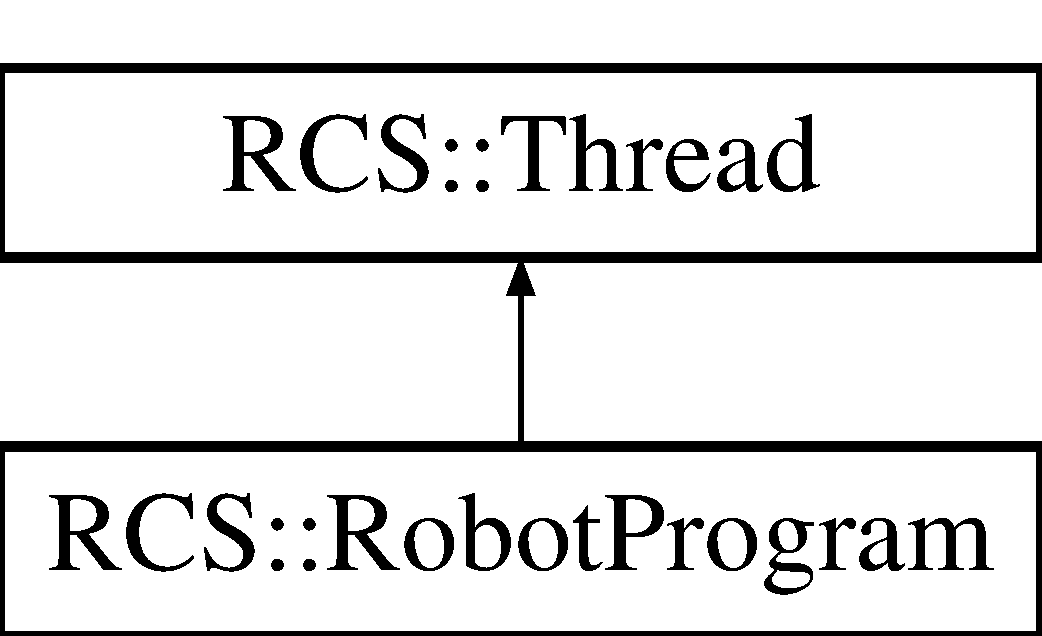
\includegraphics[height=2.000000cm]{classRCS_1_1RobotProgram}
\end{center}
\end{figure}
\subsection*{Public Member Functions}
\begin{DoxyCompactItemize}
\item 
\hyperlink{classRCS_1_1RobotProgram_a9704d21c4a2d24fc856fad7af6e99903}{Robot\-Program} (double cycletime=\hyperlink{RCS_8h_a226eb3a426e9df46b88c4ba34f217203}{D\-E\-F\-A\-U\-L\-T\-\_\-\-L\-O\-O\-P\-\_\-\-C\-Y\-C\-L\-E})
\begin{DoxyCompactList}\small\item\em \hyperlink{classRCS_1_1RobotProgram}{Robot\-Program} constructor that requires a cycle time for \hyperlink{namespaceRCS}{R\-C\-S} thread timing. \end{DoxyCompactList}\item 
virtual void \hyperlink{classRCS_1_1RobotProgram_a0998f374dd54b6a0843d33a664c9da15}{Execute\-Program} (std\-::string programpath)
\begin{DoxyCompactList}\small\item\em Execute\-Program reads a file path for C\-R\-C\-L X\-M\-L program. It will set up interpreting the program. It is thread safe. \end{DoxyCompactList}\item 
virtual void \hyperlink{classRCS_1_1RobotProgram_a637f6305bb0beea4a9140b18b245790e}{Action} ()
\begin{DoxyCompactList}\small\item\em Action is the main loop in the \hyperlink{classRCS_1_1RobotProgram}{Robot\-Program} \hyperlink{namespaceRCS}{R\-C\-S} thread. \end{DoxyCompactList}\end{DoxyCompactItemize}
\subsection*{Public Attributes}
\begin{DoxyCompactItemize}
\item 
std\-::string \hyperlink{classRCS_1_1RobotProgram_aca7d780729e20c6d4e3988883b87527d}{\-\_\-programname}
\item 
\hyperlink{classCrcl_1_1CrclDelegateInterface}{Crcl\-::\-Crcl\-Delegate\-Interface} \hyperlink{classRCS_1_1RobotProgram_addf6e9d586d1fde1aa2b8105268d9e66}{\-\_\-delegate}
\item 
std\-::istringstream \hyperlink{classRCS_1_1RobotProgram_a0099964c452870619bd0ee7651ffb072}{istr}
\item 
int \hyperlink{classRCS_1_1RobotProgram_ad43243236b573d0e3fc39d4890a43373}{cmdnum}
\item 
\-::C\-R\-C\-L\-Program\-Type\-::\-Middle\-Command\-\_\-sequence \& \hyperlink{classRCS_1_1RobotProgram_ad6ed8ea72249e836521b2f7d7feb3523}{cmds}
\end{DoxyCompactItemize}
\subsection*{Static Public Attributes}
\begin{DoxyCompactItemize}
\item 
static boost\-::mutex \hyperlink{classRCS_1_1RobotProgram_ad80469b94591e96c6a221e4769612668}{\-\_\-progmutex}
\end{DoxyCompactItemize}
\subsection*{Additional Inherited Members}


\subsection{Detailed Description}
The \hyperlink{classRCS_1_1RobotProgram}{Robot\-Program} is a thread to handle crcl programs. \hyperlink{namespaceCrcl}{Crcl} programs are not in fact legitimate, however, debugging and verification are assisted by programs. However, program as in the \hyperlink{namespaceCrcl}{Crcl} X\-S\-D specification, so it doesn't hurt to handle. They require special handling as only one command should be done at a time. Uses codesynthesis to parse \hyperlink{namespaceCrcl}{Crcl} xml into C++ data structures. 

\subsection{Constructor \& Destructor Documentation}
\hypertarget{classRCS_1_1RobotProgram_a9704d21c4a2d24fc856fad7af6e99903}{\index{R\-C\-S\-::\-Robot\-Program@{R\-C\-S\-::\-Robot\-Program}!Robot\-Program@{Robot\-Program}}
\index{Robot\-Program@{Robot\-Program}!RCS::RobotProgram@{R\-C\-S\-::\-Robot\-Program}}
\subsubsection[{Robot\-Program}]{\setlength{\rightskip}{0pt plus 5cm}R\-C\-S\-::\-Robot\-Program\-::\-Robot\-Program (
\begin{DoxyParamCaption}
\item[{double}]{cycletime = {\ttfamily {\bf D\-E\-F\-A\-U\-L\-T\-\_\-\-L\-O\-O\-P\-\_\-\-C\-Y\-C\-L\-E}}}
\end{DoxyParamCaption}
)}}\label{classRCS_1_1RobotProgram_a9704d21c4a2d24fc856fad7af6e99903}


\hyperlink{classRCS_1_1RobotProgram}{Robot\-Program} constructor that requires a cycle time for \hyperlink{namespaceRCS}{R\-C\-S} thread timing. 


\begin{DoxyParams}{Parameters}
{\em cycletime} & in seconds. \\
\hline
\end{DoxyParams}


\subsection{Member Function Documentation}
\hypertarget{classRCS_1_1RobotProgram_a637f6305bb0beea4a9140b18b245790e}{\index{R\-C\-S\-::\-Robot\-Program@{R\-C\-S\-::\-Robot\-Program}!Action@{Action}}
\index{Action@{Action}!RCS::RobotProgram@{R\-C\-S\-::\-Robot\-Program}}
\subsubsection[{Action}]{\setlength{\rightskip}{0pt plus 5cm}void R\-C\-S\-::\-Robot\-Program\-::\-Action (
\begin{DoxyParamCaption}
{}
\end{DoxyParamCaption}
)\hspace{0.3cm}{\ttfamily [virtual]}}}\label{classRCS_1_1RobotProgram_a637f6305bb0beea4a9140b18b245790e}


Action is the main loop in the \hyperlink{classRCS_1_1RobotProgram}{Robot\-Program} \hyperlink{namespaceRCS}{R\-C\-S} thread. 

Executes one program command at a time.  needs to wait until current command is done before moving on to next command. 

Reimplemented from \hyperlink{classRCS_1_1Thread_a327655d2626c51ea61bcc233a94dc78e}{R\-C\-S\-::\-Thread}.

\hypertarget{classRCS_1_1RobotProgram_a0998f374dd54b6a0843d33a664c9da15}{\index{R\-C\-S\-::\-Robot\-Program@{R\-C\-S\-::\-Robot\-Program}!Execute\-Program@{Execute\-Program}}
\index{Execute\-Program@{Execute\-Program}!RCS::RobotProgram@{R\-C\-S\-::\-Robot\-Program}}
\subsubsection[{Execute\-Program}]{\setlength{\rightskip}{0pt plus 5cm}void R\-C\-S\-::\-Robot\-Program\-::\-Execute\-Program (
\begin{DoxyParamCaption}
\item[{std\-::string}]{programpath}
\end{DoxyParamCaption}
)\hspace{0.3cm}{\ttfamily [virtual]}}}\label{classRCS_1_1RobotProgram_a0998f374dd54b6a0843d33a664c9da15}


Execute\-Program reads a file path for C\-R\-C\-L X\-M\-L program. It will set up interpreting the program. It is thread safe. 


\begin{DoxyParams}{Parameters}
{\em programpath} & path of file containing crcl xml program. \\
\hline
\end{DoxyParams}


\subsection{Member Data Documentation}
\hypertarget{classRCS_1_1RobotProgram_addf6e9d586d1fde1aa2b8105268d9e66}{\index{R\-C\-S\-::\-Robot\-Program@{R\-C\-S\-::\-Robot\-Program}!\-\_\-delegate@{\-\_\-delegate}}
\index{\-\_\-delegate@{\-\_\-delegate}!RCS::RobotProgram@{R\-C\-S\-::\-Robot\-Program}}
\subsubsection[{\-\_\-delegate}]{\setlength{\rightskip}{0pt plus 5cm}{\bf Crcl\-::\-Crcl\-Delegate\-Interface} R\-C\-S\-::\-Robot\-Program\-::\-\_\-delegate}}\label{classRCS_1_1RobotProgram_addf6e9d586d1fde1aa2b8105268d9e66}
crcl delegate used to interpret \hyperlink{namespaceCrcl}{Crcl} X\-M\-L command \hypertarget{classRCS_1_1RobotProgram_ad80469b94591e96c6a221e4769612668}{\index{R\-C\-S\-::\-Robot\-Program@{R\-C\-S\-::\-Robot\-Program}!\-\_\-progmutex@{\-\_\-progmutex}}
\index{\-\_\-progmutex@{\-\_\-progmutex}!RCS::RobotProgram@{R\-C\-S\-::\-Robot\-Program}}
\subsubsection[{\-\_\-progmutex}]{\setlength{\rightskip}{0pt plus 5cm}boost\-::mutex R\-C\-S\-::\-Robot\-Program\-::\-\_\-progmutex\hspace{0.3cm}{\ttfamily [static]}}}\label{classRCS_1_1RobotProgram_ad80469b94591e96c6a221e4769612668}
mutex for thread safe access to \hyperlink{classRCS_1_1RobotProgram}{Robot\-Program} commands \hypertarget{classRCS_1_1RobotProgram_aca7d780729e20c6d4e3988883b87527d}{\index{R\-C\-S\-::\-Robot\-Program@{R\-C\-S\-::\-Robot\-Program}!\-\_\-programname@{\-\_\-programname}}
\index{\-\_\-programname@{\-\_\-programname}!RCS::RobotProgram@{R\-C\-S\-::\-Robot\-Program}}
\subsubsection[{\-\_\-programname}]{\setlength{\rightskip}{0pt plus 5cm}std\-::string R\-C\-S\-::\-Robot\-Program\-::\-\_\-programname}}\label{classRCS_1_1RobotProgram_aca7d780729e20c6d4e3988883b87527d}
saved \hyperlink{classRCS_1_1RobotProgram}{Robot\-Program} program file path \hypertarget{classRCS_1_1RobotProgram_ad43243236b573d0e3fc39d4890a43373}{\index{R\-C\-S\-::\-Robot\-Program@{R\-C\-S\-::\-Robot\-Program}!cmdnum@{cmdnum}}
\index{cmdnum@{cmdnum}!RCS::RobotProgram@{R\-C\-S\-::\-Robot\-Program}}
\subsubsection[{cmdnum}]{\setlength{\rightskip}{0pt plus 5cm}int R\-C\-S\-::\-Robot\-Program\-::cmdnum}}\label{classRCS_1_1RobotProgram_ad43243236b573d0e3fc39d4890a43373}
number of \hyperlink{namespaceCrcl}{Crcl} X\-M\-L command to execute \hypertarget{classRCS_1_1RobotProgram_ad6ed8ea72249e836521b2f7d7feb3523}{\index{R\-C\-S\-::\-Robot\-Program@{R\-C\-S\-::\-Robot\-Program}!cmds@{cmds}}
\index{cmds@{cmds}!RCS::RobotProgram@{R\-C\-S\-::\-Robot\-Program}}
\subsubsection[{cmds}]{\setlength{\rightskip}{0pt plus 5cm}\-::C\-R\-C\-L\-Program\-Type\-::\-Middle\-Command\-\_\-sequence\& R\-C\-S\-::\-Robot\-Program\-::cmds}}\label{classRCS_1_1RobotProgram_ad6ed8ea72249e836521b2f7d7feb3523}
reference to crcl program X\-M\-L commands (from codesynthesis parsing) \hypertarget{classRCS_1_1RobotProgram_a0099964c452870619bd0ee7651ffb072}{\index{R\-C\-S\-::\-Robot\-Program@{R\-C\-S\-::\-Robot\-Program}!istr@{istr}}
\index{istr@{istr}!RCS::RobotProgram@{R\-C\-S\-::\-Robot\-Program}}
\subsubsection[{istr}]{\setlength{\rightskip}{0pt plus 5cm}std\-::istringstream R\-C\-S\-::\-Robot\-Program\-::istr}}\label{classRCS_1_1RobotProgram_a0099964c452870619bd0ee7651ffb072}
input stream interface for codesynthesis parsing 

The documentation for this class was generated from the following files\-:\begin{DoxyCompactItemize}
\item 
/home/michalos/catkin\-\_\-ws/src/nist\-\_\-fanuc/include/nist\-\_\-fanuc/\hyperlink{Controller_8h}{Controller.\-h}\item 
/home/michalos/catkin\-\_\-ws/src/nist\-\_\-fanuc/src/\hyperlink{Controller_8cpp}{Controller.\-cpp}\end{DoxyCompactItemize}

\hypertarget{classRCS_1_1RobotStatus}{\section{R\-C\-S\-:\-:Robot\-Status Class Reference}
\label{classRCS_1_1RobotStatus}\index{R\-C\-S\-::\-Robot\-Status@{R\-C\-S\-::\-Robot\-Status}}
}


The \hyperlink{classRCS_1_1RobotStatus}{Robot\-Status} is a thread that reads the status of the robot and updates the world model. The \hyperlink{classRCS_1_1RobotStatus}{Robot\-Status} is a separate thread that reads the robot status using R\-O\-S communication mechanisms and updates the controller world model based on these values. Currently, it uses an instance of the class Joint\-Reader to read joint values from the controller. It uses a Kinematics pointer reference to compute the current robot pose using the forward kinematics (F\-K) routine. It also uses a Crcl\-Delegate pointer reference to update the status reported by C\-R\-C\-L.  




{\ttfamily \#include $<$Controller.\-h$>$}

Inheritance diagram for R\-C\-S\-:\-:Robot\-Status\-:\begin{figure}[H]
\begin{center}
\leavevmode
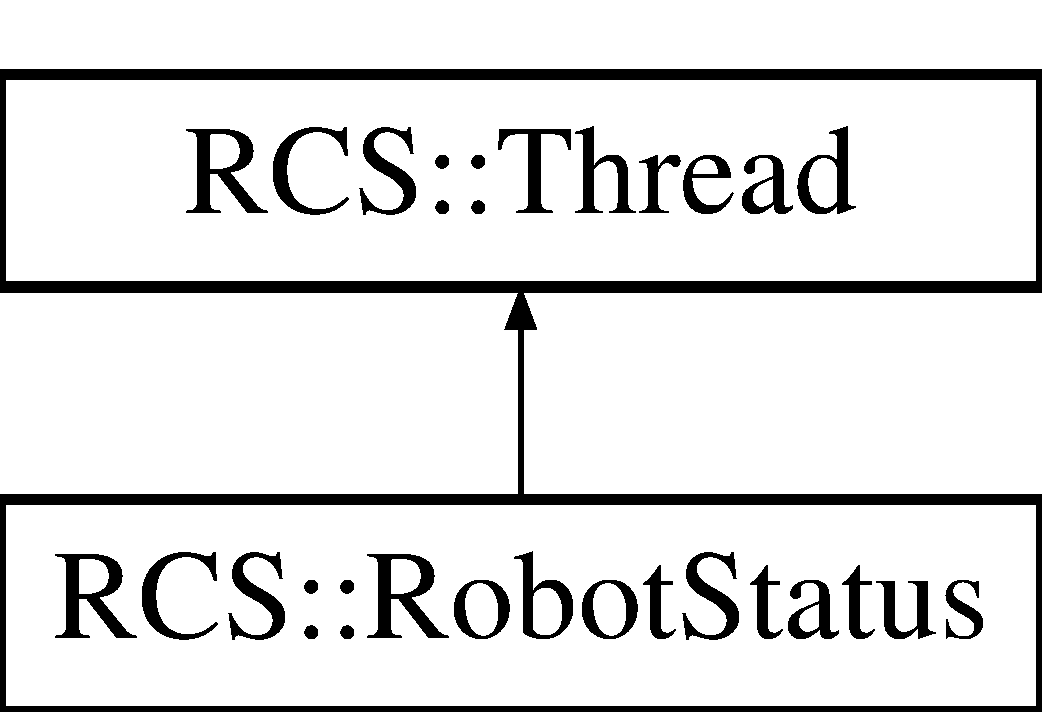
\includegraphics[height=2.000000cm]{classRCS_1_1RobotStatus}
\end{center}
\end{figure}
\subsection*{Public Member Functions}
\begin{DoxyCompactItemize}
\item 
\hyperlink{classRCS_1_1RobotStatus_a3a4edecf6814bd37db609104517983a1}{Robot\-Status} (double cycletime=\hyperlink{RCS_8h_a226eb3a426e9df46b88c4ba34f217203}{D\-E\-F\-A\-U\-L\-T\-\_\-\-L\-O\-O\-P\-\_\-\-C\-Y\-C\-L\-E})
\begin{DoxyCompactList}\small\item\em \hyperlink{classRCS_1_1RobotStatus}{Robot\-Status} constructor that requires a cycle time for \hyperlink{namespaceRCS}{R\-C\-S} thread timing. \end{DoxyCompactList}\item 
\hyperlink{classRCS_1_1RobotStatus_aed67d1057ff99ebe1221aa9fdc3c9e04}{N\-V\-A\-R} (Crcl\-Delegate, boost\-::shared\-\_\-ptr$<$ \hyperlink{classCrcl_1_1CrclDelegateInterface}{Crcl\-::\-Crcl\-Delegate\-Interface} $>$, \-\_\-crclinterface)
\item 
\hyperlink{classRCS_1_1RobotStatus_abd9c969c564c66c5dd4ae92699172742}{V\-A\-R} (Joint\-Reader, boost\-::shared\-\_\-ptr$<$ \hyperlink{classCJointReader}{C\-Joint\-Reader} $>$)
\item 
\hyperlink{classRCS_1_1RobotStatus_abdcfb3be4ed2558ca3e5c745dc669340}{V\-A\-R} (\hyperlink{SanityCheckTests_8cpp_ac2d60ae645ce73be6021c92b37789e7c}{Kinematics}, boost\-::shared\-\_\-ptr$<$ \hyperlink{classIKinematics}{I\-Kinematics} $>$)
\item 
virtual void \hyperlink{classRCS_1_1RobotStatus_a7b8484b6d7ad5ae10e41a5d327efc658}{Action} ()
\begin{DoxyCompactList}\small\item\em Action is the main loop in the \hyperlink{namespaceRCS}{R\-C\-S} thread timing. Get latest robot joint readings. Use forward kinematics to get current pose. Then, updates the C\-R\-C\-L world model with the latest readings.  Should it keep track of the command id also -\/ in theory only one C\-R\-Cl command at a time. \end{DoxyCompactList}\item 
bool \hyperlink{classRCS_1_1RobotStatus_aad11542a68b43feb8c327abafbd94344}{Verify} ()
\begin{DoxyCompactList}\small\item\em method to determine if the instance is valid, i.\-e., has all reference pointers. \end{DoxyCompactList}\end{DoxyCompactItemize}
\subsection*{Additional Inherited Members}


\subsection{Detailed Description}
The \hyperlink{classRCS_1_1RobotStatus}{Robot\-Status} is a thread that reads the status of the robot and updates the world model. The \hyperlink{classRCS_1_1RobotStatus}{Robot\-Status} is a separate thread that reads the robot status using R\-O\-S communication mechanisms and updates the controller world model based on these values. Currently, it uses an instance of the class Joint\-Reader to read joint values from the controller. It uses a Kinematics pointer reference to compute the current robot pose using the forward kinematics (F\-K) routine. It also uses a Crcl\-Delegate pointer reference to update the status reported by C\-R\-C\-L. 

\subsection{Constructor \& Destructor Documentation}
\hypertarget{classRCS_1_1RobotStatus_a3a4edecf6814bd37db609104517983a1}{\index{R\-C\-S\-::\-Robot\-Status@{R\-C\-S\-::\-Robot\-Status}!Robot\-Status@{Robot\-Status}}
\index{Robot\-Status@{Robot\-Status}!RCS::RobotStatus@{R\-C\-S\-::\-Robot\-Status}}
\subsubsection[{Robot\-Status}]{\setlength{\rightskip}{0pt plus 5cm}R\-C\-S\-::\-Robot\-Status\-::\-Robot\-Status (
\begin{DoxyParamCaption}
\item[{double}]{cycletime = {\ttfamily {\bf D\-E\-F\-A\-U\-L\-T\-\_\-\-L\-O\-O\-P\-\_\-\-C\-Y\-C\-L\-E}}}
\end{DoxyParamCaption}
)}}\label{classRCS_1_1RobotStatus_a3a4edecf6814bd37db609104517983a1}


\hyperlink{classRCS_1_1RobotStatus}{Robot\-Status} constructor that requires a cycle time for \hyperlink{namespaceRCS}{R\-C\-S} thread timing. 


\begin{DoxyParams}{Parameters}
{\em cycletime} & in seconds. \\
\hline
\end{DoxyParams}


\subsection{Member Function Documentation}
\hypertarget{classRCS_1_1RobotStatus_a7b8484b6d7ad5ae10e41a5d327efc658}{\index{R\-C\-S\-::\-Robot\-Status@{R\-C\-S\-::\-Robot\-Status}!Action@{Action}}
\index{Action@{Action}!RCS::RobotStatus@{R\-C\-S\-::\-Robot\-Status}}
\subsubsection[{Action}]{\setlength{\rightskip}{0pt plus 5cm}void R\-C\-S\-::\-Robot\-Status\-::\-Action (
\begin{DoxyParamCaption}
{}
\end{DoxyParamCaption}
)\hspace{0.3cm}{\ttfamily [virtual]}}}\label{classRCS_1_1RobotStatus_a7b8484b6d7ad5ae10e41a5d327efc658}


Action is the main loop in the \hyperlink{namespaceRCS}{R\-C\-S} thread timing. Get latest robot joint readings. Use forward kinematics to get current pose. Then, updates the C\-R\-C\-L world model with the latest readings.  Should it keep track of the command id also -\/ in theory only one C\-R\-Cl command at a time. 



Reimplemented from \hyperlink{classRCS_1_1Thread_a327655d2626c51ea61bcc233a94dc78e}{R\-C\-S\-::\-Thread}.

\hypertarget{classRCS_1_1RobotStatus_aed67d1057ff99ebe1221aa9fdc3c9e04}{\index{R\-C\-S\-::\-Robot\-Status@{R\-C\-S\-::\-Robot\-Status}!N\-V\-A\-R@{N\-V\-A\-R}}
\index{N\-V\-A\-R@{N\-V\-A\-R}!RCS::RobotStatus@{R\-C\-S\-::\-Robot\-Status}}
\subsubsection[{N\-V\-A\-R}]{\setlength{\rightskip}{0pt plus 5cm}R\-C\-S\-::\-Robot\-Status\-::\-N\-V\-A\-R (
\begin{DoxyParamCaption}
\item[{Crcl\-Delegate}]{, }
\item[{boost\-::shared\-\_\-ptr$<$ {\bf Crcl\-::\-Crcl\-Delegate\-Interface} $>$}]{, }
\item[{\-\_\-crclinterface}]{}
\end{DoxyParamCaption}
)}}\label{classRCS_1_1RobotStatus_aed67d1057ff99ebe1221aa9fdc3c9e04}
\hypertarget{classRCS_1_1RobotStatus_abd9c969c564c66c5dd4ae92699172742}{\index{R\-C\-S\-::\-Robot\-Status@{R\-C\-S\-::\-Robot\-Status}!V\-A\-R@{V\-A\-R}}
\index{V\-A\-R@{V\-A\-R}!RCS::RobotStatus@{R\-C\-S\-::\-Robot\-Status}}
\subsubsection[{V\-A\-R}]{\setlength{\rightskip}{0pt plus 5cm}R\-C\-S\-::\-Robot\-Status\-::\-V\-A\-R (
\begin{DoxyParamCaption}
\item[{Joint\-Reader}]{, }
\item[{boost\-::shared\-\_\-ptr$<$ {\bf C\-Joint\-Reader} $>$}]{}
\end{DoxyParamCaption}
)}}\label{classRCS_1_1RobotStatus_abd9c969c564c66c5dd4ae92699172742}
\hypertarget{classRCS_1_1RobotStatus_abdcfb3be4ed2558ca3e5c745dc669340}{\index{R\-C\-S\-::\-Robot\-Status@{R\-C\-S\-::\-Robot\-Status}!V\-A\-R@{V\-A\-R}}
\index{V\-A\-R@{V\-A\-R}!RCS::RobotStatus@{R\-C\-S\-::\-Robot\-Status}}
\subsubsection[{V\-A\-R}]{\setlength{\rightskip}{0pt plus 5cm}R\-C\-S\-::\-Robot\-Status\-::\-V\-A\-R (
\begin{DoxyParamCaption}
\item[{{\bf Kinematics}}]{, }
\item[{boost\-::shared\-\_\-ptr$<$ {\bf I\-Kinematics} $>$}]{}
\end{DoxyParamCaption}
)}}\label{classRCS_1_1RobotStatus_abdcfb3be4ed2558ca3e5c745dc669340}
\hypertarget{classRCS_1_1RobotStatus_aad11542a68b43feb8c327abafbd94344}{\index{R\-C\-S\-::\-Robot\-Status@{R\-C\-S\-::\-Robot\-Status}!Verify@{Verify}}
\index{Verify@{Verify}!RCS::RobotStatus@{R\-C\-S\-::\-Robot\-Status}}
\subsubsection[{Verify}]{\setlength{\rightskip}{0pt plus 5cm}bool R\-C\-S\-::\-Robot\-Status\-::\-Verify (
\begin{DoxyParamCaption}
{}
\end{DoxyParamCaption}
)\hspace{0.3cm}{\ttfamily [inline]}}}\label{classRCS_1_1RobotStatus_aad11542a68b43feb8c327abafbd94344}


method to determine if the instance is valid, i.\-e., has all reference pointers. 

\begin{DoxyReturn}{Returns}
boolean to signify whether component is valid. 
\end{DoxyReturn}


The documentation for this class was generated from the following files\-:\begin{DoxyCompactItemize}
\item 
/home/michalos/catkin\-\_\-ws/src/nist\-\_\-fanuc/include/nist\-\_\-fanuc/\hyperlink{Controller_8h}{Controller.\-h}\item 
/home/michalos/catkin\-\_\-ws/src/nist\-\_\-fanuc/src/\hyperlink{Controller_8cpp}{Controller.\-cpp}\end{DoxyCompactItemize}

\hypertarget{classRosKinematics}{\section{Ros\-Kinematics Class Reference}
\label{classRosKinematics}\index{Ros\-Kinematics@{Ros\-Kinematics}}
}


The \hyperlink{classRosKinematics}{Ros\-Kinematics} class instantiates the \hyperlink{classIKinematics}{I\-Kinematics} abstract class and fills in the pure virtual functions with Descartes kinematic methods.  




{\ttfamily \#include $<$Kinematics.\-h$>$}

Inheritance diagram for Ros\-Kinematics\-:\begin{figure}[H]
\begin{center}
\leavevmode
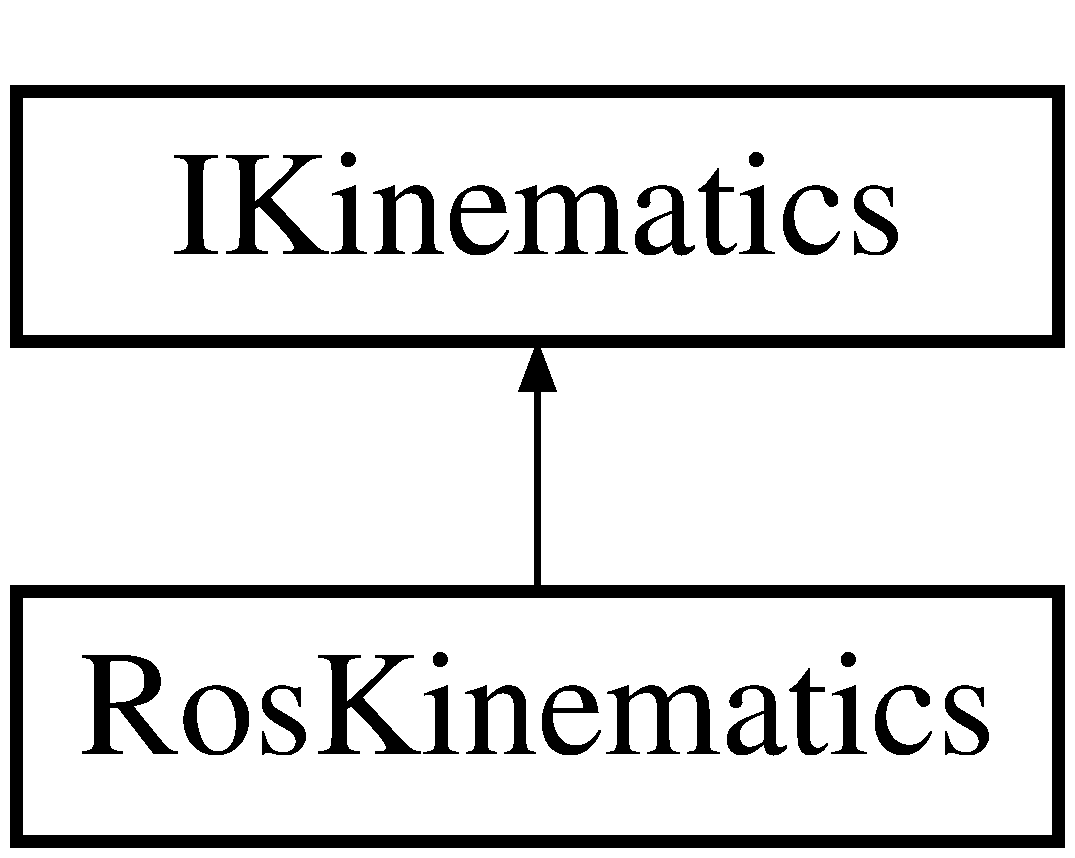
\includegraphics[height=2.000000cm]{classRosKinematics}
\end{center}
\end{figure}
\subsection*{Public Member Functions}
\begin{DoxyCompactItemize}
\item 
\hyperlink{classRosKinematics_a9dc704b4556f6db399ad18cea7d6259b}{Ros\-Kinematics} ()
\item 
virtual void \hyperlink{classRosKinematics_a307da5d4456621c4cc2dce412be30db3}{Init} (std\-::string groupname, std\-::string eelinkname)
\begin{DoxyCompactList}\small\item\em Init is necessary for R\-O\-S to initialize it kinematics using robot model . \end{DoxyCompactList}\item 
virtual std\-::vector$<$ double $>$ \hyperlink{classRosKinematics_ab3e293c7f5d7220fa7ee91256321ec92}{Get\-Joint\-Values} ()
\begin{DoxyCompactList}\small\item\em Get\-Joint\-Values returns latest reading of end effector. \end{DoxyCompactList}\item 
void \hyperlink{classRosKinematics_af9af8957f54e5d2343b2ab00dcb55525}{Set\-Joint\-Values} (std\-::vector$<$ double $>$ \hyperlink{classRosKinematics_af95c3ba0edaccafeb68022895b9824ac}{joint\-\_\-values})
\begin{DoxyCompactList}\small\item\em Set\-Joint\-Values sets the latest joint values of the robot. \end{DoxyCompactList}\item 
virtual \hyperlink{namespaceRCS_aa07e45d8a50e30064283d2b38087f999}{R\-C\-S\-::\-Pose} \hyperlink{classRosKinematics_a1b0ea6900e6da0aa888d4f4c2a23b445}{F\-K} (std\-::vector$<$ double $>$ jv)
\begin{DoxyCompactList}\small\item\em F\-K performs the forward kinematics using the joint values of the robot provided. \end{DoxyCompactList}\item 
virtual std\-::vector$<$ double $>$ \hyperlink{classRosKinematics_ae8f76a870595ca94d3876bbe51c7b142}{I\-K} (\hyperlink{namespaceRCS_aa07e45d8a50e30064283d2b38087f999}{R\-C\-S\-::\-Pose} \&pose, std\-::vector$<$ double $>$ oldjoints)
\begin{DoxyCompactList}\small\item\em I\-K performs the inverse kinematics using the Cartesian pose provided. \end{DoxyCompactList}\item 
bool \hyperlink{classRosKinematics_ae51c062c810983b29d418399d38da42f}{Satisfies\-Bounds} ()
\item 
void \hyperlink{classRosKinematics_a19e0993e7e188491918785f4ca6ce115}{Enforce\-Bounds} ()
\item 
virtual size\-\_\-t \hyperlink{classRosKinematics_ae3d78b75e8cbd38a12d451e0e0e95548}{All\-Pose\-To\-Joints} (\hyperlink{namespaceRCS_aa07e45d8a50e30064283d2b38087f999}{R\-C\-S\-::\-Pose} \&pose, std\-::vector$<$ std\-::vector$<$ double $>$ $>$ \&newjoints)
\begin{DoxyCompactList}\small\item\em All\-Pose\-To\-Joints solves the inverse kinematics to find all solutions using the Cartesian pose provided. \end{DoxyCompactList}\item 
virtual std\-::vector$<$ double $>$ \hyperlink{classRosKinematics_ab50d3e7666cf3b2bdb1ae3d5e0a7db8e}{Nearest\-Joints} (std\-::vector$<$ double $>$ oldjoints, std\-::vector$<$ std\-::vector$<$ double $>$ $>$ \&newjoints)
\begin{DoxyCompactList}\small\item\em Nearest\-Joints finds the joint set that is closest to the old joints. \end{DoxyCompactList}\end{DoxyCompactItemize}
\subsection*{Public Attributes}
\begin{DoxyCompactItemize}
\item 
robot\-\_\-model\-::\-Robot\-Model\-Ptr \hyperlink{classRosKinematics_a0ab6cd969d40fa1e40707e8982f76f15}{kinematic\-\_\-model}
\item 
robot\-\_\-state\-::\-Robot\-State\-Ptr \hyperlink{classRosKinematics_a2236796eba89e23f8b47b6fcd87a296d}{kinematic\-\_\-state}
\item 
robot\-\_\-state\-::\-Joint\-Model\-Group $\ast$ \hyperlink{classRosKinematics_ab6f642bac05e91ab8cf0675232e4cf1b}{joint\-\_\-model\-\_\-group}
\item 
std\-::vector$<$ double $>$ \hyperlink{classRosKinematics_af95c3ba0edaccafeb68022895b9824ac}{joint\-\_\-values}
\item 
std\-::vector$<$ std\-::string $>$ \hyperlink{classRosKinematics_a0690908a8ee72e65685dc5b0a0da00df}{joint\-\_\-names}
\item 
std\-::string \hyperlink{classRosKinematics_a80fac3df36e85d02b79c83a35e961f78}{\-\_\-groupname}
\item 
std\-::string \hyperlink{classRosKinematics_ad2aeb76b94edd1bdfb4830eacadebd61}{\-\_\-eelinkname}
\item 
bool \hyperlink{classRosKinematics_a3cae7f7ad57a5df821c2ebf8b55057d5}{\-\_\-b\-Init}
\item 
boost\-::mutex \hyperlink{classRosKinematics_a79f88926f9403d9b90cad26d0fa43193}{kinmutex}
\end{DoxyCompactItemize}


\subsection{Detailed Description}
The \hyperlink{classRosKinematics}{Ros\-Kinematics} class instantiates the \hyperlink{classIKinematics}{I\-Kinematics} abstract class and fills in the pure virtual functions with Descartes kinematic methods. 

\subsection{Constructor \& Destructor Documentation}
\hypertarget{classRosKinematics_a9dc704b4556f6db399ad18cea7d6259b}{\index{Ros\-Kinematics@{Ros\-Kinematics}!Ros\-Kinematics@{Ros\-Kinematics}}
\index{Ros\-Kinematics@{Ros\-Kinematics}!RosKinematics@{Ros\-Kinematics}}
\subsubsection[{Ros\-Kinematics}]{\setlength{\rightskip}{0pt plus 5cm}Ros\-Kinematics\-::\-Ros\-Kinematics (
\begin{DoxyParamCaption}
{}
\end{DoxyParamCaption}
)}}\label{classRosKinematics_a9dc704b4556f6db399ad18cea7d6259b}


\subsection{Member Function Documentation}
\hypertarget{classRosKinematics_ae3d78b75e8cbd38a12d451e0e0e95548}{\index{Ros\-Kinematics@{Ros\-Kinematics}!All\-Pose\-To\-Joints@{All\-Pose\-To\-Joints}}
\index{All\-Pose\-To\-Joints@{All\-Pose\-To\-Joints}!RosKinematics@{Ros\-Kinematics}}
\subsubsection[{All\-Pose\-To\-Joints}]{\setlength{\rightskip}{0pt plus 5cm}virtual size\-\_\-t Ros\-Kinematics\-::\-All\-Pose\-To\-Joints (
\begin{DoxyParamCaption}
\item[{{\bf R\-C\-S\-::\-Pose} \&}]{pose, }
\item[{std\-::vector$<$ std\-::vector$<$ double $>$ $>$ \&}]{newjoints}
\end{DoxyParamCaption}
)\hspace{0.3cm}{\ttfamily [inline]}, {\ttfamily [virtual]}}}\label{classRosKinematics_ae3d78b75e8cbd38a12d451e0e0e95548}


All\-Pose\-To\-Joints solves the inverse kinematics to find all solutions using the Cartesian pose provided. 


\begin{DoxyParams}{Parameters}
{\em Cartesian} & robot pose of end effector. \\
\hline
{\em vector} & of double vectos to hold all the I\-K joint solutions. \\
\hline
\end{DoxyParams}
\begin{DoxyReturn}{Returns}
number of solutions found. 
\end{DoxyReturn}


Implements \hyperlink{classIKinematics_aeb53bb4b2a1e70a79d5d724e5eb82c10}{I\-Kinematics}.

\hypertarget{classRosKinematics_a19e0993e7e188491918785f4ca6ce115}{\index{Ros\-Kinematics@{Ros\-Kinematics}!Enforce\-Bounds@{Enforce\-Bounds}}
\index{Enforce\-Bounds@{Enforce\-Bounds}!RosKinematics@{Ros\-Kinematics}}
\subsubsection[{Enforce\-Bounds}]{\setlength{\rightskip}{0pt plus 5cm}void Ros\-Kinematics\-::\-Enforce\-Bounds (
\begin{DoxyParamCaption}
{}
\end{DoxyParamCaption}
)}}\label{classRosKinematics_a19e0993e7e188491918785f4ca6ce115}
\hypertarget{classRosKinematics_a1b0ea6900e6da0aa888d4f4c2a23b445}{\index{Ros\-Kinematics@{Ros\-Kinematics}!F\-K@{F\-K}}
\index{F\-K@{F\-K}!RosKinematics@{Ros\-Kinematics}}
\subsubsection[{F\-K}]{\setlength{\rightskip}{0pt plus 5cm}{\bf R\-C\-S\-::\-Pose} Ros\-Kinematics\-::\-F\-K (
\begin{DoxyParamCaption}
\item[{std\-::vector$<$ double $>$}]{jv}
\end{DoxyParamCaption}
)\hspace{0.3cm}{\ttfamily [virtual]}}}\label{classRosKinematics_a1b0ea6900e6da0aa888d4f4c2a23b445}


F\-K performs the forward kinematics using the joint values of the robot provided. 


\begin{DoxyParams}{Parameters}
{\em vector} & of all robot joint values in doubles. \\
\hline
\end{DoxyParams}
\begin{DoxyReturn}{Returns}
corresponding Cartesian robot pose of end effector. 
\end{DoxyReturn}


Implements \hyperlink{classIKinematics_abf765053ac39fac5b94ef99e80b17f1b}{I\-Kinematics}.

\hypertarget{classRosKinematics_ab3e293c7f5d7220fa7ee91256321ec92}{\index{Ros\-Kinematics@{Ros\-Kinematics}!Get\-Joint\-Values@{Get\-Joint\-Values}}
\index{Get\-Joint\-Values@{Get\-Joint\-Values}!RosKinematics@{Ros\-Kinematics}}
\subsubsection[{Get\-Joint\-Values}]{\setlength{\rightskip}{0pt plus 5cm}std\-::vector$<$ double $>$ Ros\-Kinematics\-::\-Get\-Joint\-Values (
\begin{DoxyParamCaption}
{}
\end{DoxyParamCaption}
)\hspace{0.3cm}{\ttfamily [virtual]}}}\label{classRosKinematics_ab3e293c7f5d7220fa7ee91256321ec92}


Get\-Joint\-Values returns latest reading of end effector. 

\begin{DoxyReturn}{Returns}
vector of joint values in doubles. 
\end{DoxyReturn}


Implements \hyperlink{classIKinematics_af41a85f8dc0cac9d94f982c7cf58b475}{I\-Kinematics}.

\hypertarget{classRosKinematics_ae8f76a870595ca94d3876bbe51c7b142}{\index{Ros\-Kinematics@{Ros\-Kinematics}!I\-K@{I\-K}}
\index{I\-K@{I\-K}!RosKinematics@{Ros\-Kinematics}}
\subsubsection[{I\-K}]{\setlength{\rightskip}{0pt plus 5cm}std\-::vector$<$ double $>$ Ros\-Kinematics\-::\-I\-K (
\begin{DoxyParamCaption}
\item[{{\bf R\-C\-S\-::\-Pose} \&}]{pose, }
\item[{std\-::vector$<$ double $>$}]{oldjoints}
\end{DoxyParamCaption}
)\hspace{0.3cm}{\ttfamily [virtual]}}}\label{classRosKinematics_ae8f76a870595ca94d3876bbe51c7b142}


I\-K performs the inverse kinematics using the Cartesian pose provided. 


\begin{DoxyParams}{Parameters}
{\em Cartesian} & robot pose of end effector. \\
\hline
{\em optional} & seed joint values to use as best guess for I\-K joint values. \\
\hline
\end{DoxyParams}
\begin{DoxyReturn}{Returns}
vector of all robot joint values in doubles. 
\end{DoxyReturn}


Implements \hyperlink{classIKinematics_ad0715c776a7eb325d2543bc34fa8114f}{I\-Kinematics}.

\hypertarget{classRosKinematics_a307da5d4456621c4cc2dce412be30db3}{\index{Ros\-Kinematics@{Ros\-Kinematics}!Init@{Init}}
\index{Init@{Init}!RosKinematics@{Ros\-Kinematics}}
\subsubsection[{Init}]{\setlength{\rightskip}{0pt plus 5cm}void Ros\-Kinematics\-::\-Init (
\begin{DoxyParamCaption}
\item[{std\-::string}]{groupname, }
\item[{std\-::string}]{eelinkname}
\end{DoxyParamCaption}
)\hspace{0.3cm}{\ttfamily [virtual]}}}\label{classRosKinematics_a307da5d4456621c4cc2dce412be30db3}


Init is necessary for R\-O\-S to initialize it kinematics using robot model . 


\begin{DoxyParams}{Parameters}
{\em groupname} & name of chained joints in robot model. \\
\hline
{\em eelinkname} & name of end effector joint in robot model. \\
\hline
\end{DoxyParams}


Reimplemented from \hyperlink{classIKinematics_a1407620d6cf7f26e61a64af42d570b8f}{I\-Kinematics}.

\hypertarget{classRosKinematics_ab50d3e7666cf3b2bdb1ae3d5e0a7db8e}{\index{Ros\-Kinematics@{Ros\-Kinematics}!Nearest\-Joints@{Nearest\-Joints}}
\index{Nearest\-Joints@{Nearest\-Joints}!RosKinematics@{Ros\-Kinematics}}
\subsubsection[{Nearest\-Joints}]{\setlength{\rightskip}{0pt plus 5cm}virtual std\-::vector$<$double$>$ Ros\-Kinematics\-::\-Nearest\-Joints (
\begin{DoxyParamCaption}
\item[{std\-::vector$<$ double $>$}]{oldjoints, }
\item[{std\-::vector$<$ std\-::vector$<$ double $>$ $>$ \&}]{newjoints}
\end{DoxyParamCaption}
)\hspace{0.3cm}{\ttfamily [inline]}, {\ttfamily [virtual]}}}\label{classRosKinematics_ab50d3e7666cf3b2bdb1ae3d5e0a7db8e}


Nearest\-Joints finds the joint set that is closest to the old joints. 


\begin{DoxyParams}{Parameters}
{\em old} & seed joint values to use as best guess for I\-K joint values. \\
\hline
{\em vector} & of double vectos that holds all the I\-K joint solutions. \\
\hline
\end{DoxyParams}
\begin{DoxyReturn}{Returns}
vector of doubles with closest set to seed joints. 
\end{DoxyReturn}


Implements \hyperlink{classIKinematics_ab74b70ed6ecc53adfc36505b8dd1fef4}{I\-Kinematics}.

\hypertarget{classRosKinematics_ae51c062c810983b29d418399d38da42f}{\index{Ros\-Kinematics@{Ros\-Kinematics}!Satisfies\-Bounds@{Satisfies\-Bounds}}
\index{Satisfies\-Bounds@{Satisfies\-Bounds}!RosKinematics@{Ros\-Kinematics}}
\subsubsection[{Satisfies\-Bounds}]{\setlength{\rightskip}{0pt plus 5cm}bool Ros\-Kinematics\-::\-Satisfies\-Bounds (
\begin{DoxyParamCaption}
{}
\end{DoxyParamCaption}
)}}\label{classRosKinematics_ae51c062c810983b29d418399d38da42f}
\hypertarget{classRosKinematics_af9af8957f54e5d2343b2ab00dcb55525}{\index{Ros\-Kinematics@{Ros\-Kinematics}!Set\-Joint\-Values@{Set\-Joint\-Values}}
\index{Set\-Joint\-Values@{Set\-Joint\-Values}!RosKinematics@{Ros\-Kinematics}}
\subsubsection[{Set\-Joint\-Values}]{\setlength{\rightskip}{0pt plus 5cm}void Ros\-Kinematics\-::\-Set\-Joint\-Values (
\begin{DoxyParamCaption}
\item[{std\-::vector$<$ double $>$}]{joint\-\_\-values}
\end{DoxyParamCaption}
)\hspace{0.3cm}{\ttfamily [virtual]}}}\label{classRosKinematics_af9af8957f54e5d2343b2ab00dcb55525}


Set\-Joint\-Values sets the latest joint values of the robot. 


\begin{DoxyParams}{Parameters}
{\em vector} & of all robot joint values in doubles. \\
\hline
\end{DoxyParams}


Implements \hyperlink{classIKinematics_ad43b2185f06e20eb0bf9d5a94d4aec18}{I\-Kinematics}.



\subsection{Member Data Documentation}
\hypertarget{classRosKinematics_a3cae7f7ad57a5df821c2ebf8b55057d5}{\index{Ros\-Kinematics@{Ros\-Kinematics}!\-\_\-b\-Init@{\-\_\-b\-Init}}
\index{\-\_\-b\-Init@{\-\_\-b\-Init}!RosKinematics@{Ros\-Kinematics}}
\subsubsection[{\-\_\-b\-Init}]{\setlength{\rightskip}{0pt plus 5cm}bool Ros\-Kinematics\-::\-\_\-b\-Init}}\label{classRosKinematics_a3cae7f7ad57a5df821c2ebf8b55057d5}
\hypertarget{classRosKinematics_ad2aeb76b94edd1bdfb4830eacadebd61}{\index{Ros\-Kinematics@{Ros\-Kinematics}!\-\_\-eelinkname@{\-\_\-eelinkname}}
\index{\-\_\-eelinkname@{\-\_\-eelinkname}!RosKinematics@{Ros\-Kinematics}}
\subsubsection[{\-\_\-eelinkname}]{\setlength{\rightskip}{0pt plus 5cm}std\-::string Ros\-Kinematics\-::\-\_\-eelinkname}}\label{classRosKinematics_ad2aeb76b94edd1bdfb4830eacadebd61}
\hypertarget{classRosKinematics_a80fac3df36e85d02b79c83a35e961f78}{\index{Ros\-Kinematics@{Ros\-Kinematics}!\-\_\-groupname@{\-\_\-groupname}}
\index{\-\_\-groupname@{\-\_\-groupname}!RosKinematics@{Ros\-Kinematics}}
\subsubsection[{\-\_\-groupname}]{\setlength{\rightskip}{0pt plus 5cm}std\-::string Ros\-Kinematics\-::\-\_\-groupname}}\label{classRosKinematics_a80fac3df36e85d02b79c83a35e961f78}
\hypertarget{classRosKinematics_ab6f642bac05e91ab8cf0675232e4cf1b}{\index{Ros\-Kinematics@{Ros\-Kinematics}!joint\-\_\-model\-\_\-group@{joint\-\_\-model\-\_\-group}}
\index{joint\-\_\-model\-\_\-group@{joint\-\_\-model\-\_\-group}!RosKinematics@{Ros\-Kinematics}}
\subsubsection[{joint\-\_\-model\-\_\-group}]{\setlength{\rightskip}{0pt plus 5cm}robot\-\_\-state\-::\-Joint\-Model\-Group$\ast$ Ros\-Kinematics\-::joint\-\_\-model\-\_\-group}}\label{classRosKinematics_ab6f642bac05e91ab8cf0675232e4cf1b}
\hypertarget{classRosKinematics_a0690908a8ee72e65685dc5b0a0da00df}{\index{Ros\-Kinematics@{Ros\-Kinematics}!joint\-\_\-names@{joint\-\_\-names}}
\index{joint\-\_\-names@{joint\-\_\-names}!RosKinematics@{Ros\-Kinematics}}
\subsubsection[{joint\-\_\-names}]{\setlength{\rightskip}{0pt plus 5cm}std\-::vector$<$std\-::string$>$ Ros\-Kinematics\-::joint\-\_\-names}}\label{classRosKinematics_a0690908a8ee72e65685dc5b0a0da00df}
\hypertarget{classRosKinematics_af95c3ba0edaccafeb68022895b9824ac}{\index{Ros\-Kinematics@{Ros\-Kinematics}!joint\-\_\-values@{joint\-\_\-values}}
\index{joint\-\_\-values@{joint\-\_\-values}!RosKinematics@{Ros\-Kinematics}}
\subsubsection[{joint\-\_\-values}]{\setlength{\rightskip}{0pt plus 5cm}std\-::vector$<$double$>$ Ros\-Kinematics\-::joint\-\_\-values}}\label{classRosKinematics_af95c3ba0edaccafeb68022895b9824ac}
\hypertarget{classRosKinematics_a0ab6cd969d40fa1e40707e8982f76f15}{\index{Ros\-Kinematics@{Ros\-Kinematics}!kinematic\-\_\-model@{kinematic\-\_\-model}}
\index{kinematic\-\_\-model@{kinematic\-\_\-model}!RosKinematics@{Ros\-Kinematics}}
\subsubsection[{kinematic\-\_\-model}]{\setlength{\rightskip}{0pt plus 5cm}robot\-\_\-model\-::\-Robot\-Model\-Ptr Ros\-Kinematics\-::kinematic\-\_\-model}}\label{classRosKinematics_a0ab6cd969d40fa1e40707e8982f76f15}
\hypertarget{classRosKinematics_a2236796eba89e23f8b47b6fcd87a296d}{\index{Ros\-Kinematics@{Ros\-Kinematics}!kinematic\-\_\-state@{kinematic\-\_\-state}}
\index{kinematic\-\_\-state@{kinematic\-\_\-state}!RosKinematics@{Ros\-Kinematics}}
\subsubsection[{kinematic\-\_\-state}]{\setlength{\rightskip}{0pt plus 5cm}robot\-\_\-state\-::\-Robot\-State\-Ptr Ros\-Kinematics\-::kinematic\-\_\-state}}\label{classRosKinematics_a2236796eba89e23f8b47b6fcd87a296d}
\hypertarget{classRosKinematics_a79f88926f9403d9b90cad26d0fa43193}{\index{Ros\-Kinematics@{Ros\-Kinematics}!kinmutex@{kinmutex}}
\index{kinmutex@{kinmutex}!RosKinematics@{Ros\-Kinematics}}
\subsubsection[{kinmutex}]{\setlength{\rightskip}{0pt plus 5cm}boost\-::mutex Ros\-Kinematics\-::kinmutex}}\label{classRosKinematics_a79f88926f9403d9b90cad26d0fa43193}


The documentation for this class was generated from the following files\-:\begin{DoxyCompactItemize}
\item 
/home/michalos/catkin\-\_\-ws/src/nist\-\_\-fanuc/include/nist\-\_\-fanuc/\hyperlink{Kinematics_8h}{Kinematics.\-h}\item 
/home/michalos/catkin\-\_\-ws/src/nist\-\_\-fanuc/src/\hyperlink{Kinematics_8cpp}{Kinematics.\-cpp}\end{DoxyCompactItemize}

\hypertarget{classRCS_1_1Thread}{\section{R\-C\-S\-:\-:Thread Class Reference}
\label{classRCS_1_1Thread}\index{R\-C\-S\-::\-Thread@{R\-C\-S\-::\-Thread}}
}


\hyperlink{classRCS_1_1Thread}{Thread} is an \hyperlink{namespaceRCS}{R\-C\-S} ulapi equivalent for a timed thread. Given a cycle time, the thread provides a wait function to sleep to exactly the amount of the thread cycle time. It keeps track of busy/idle time for diagnostic purposes. \par
 Notes\-: \href{https://www.quantnet.com/threads/c-multithreading-in-boost.10028/}{\tt https\-://www.\-quantnet.\-com/threads/c-\/multithreading-\/in-\/boost.\-10028/}.  




{\ttfamily \#include $<$R\-C\-S\-Thread\-Template.\-h$>$}

Inheritance diagram for R\-C\-S\-:\-:Thread\-:\begin{figure}[H]
\begin{center}
\leavevmode
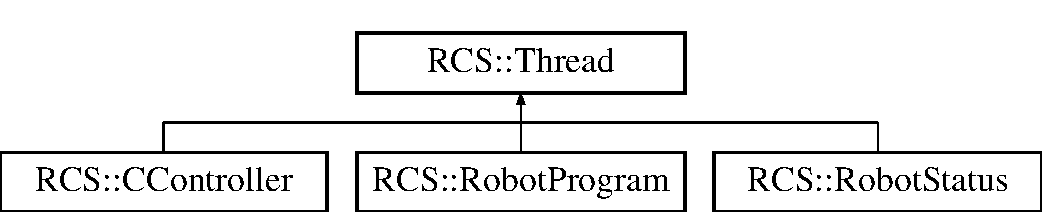
\includegraphics[height=2.000000cm]{classRCS_1_1Thread}
\end{center}
\end{figure}
\subsection*{Public Member Functions}
\begin{DoxyCompactItemize}
\item 
\hyperlink{classRCS_1_1Thread_a3f5e86f11c0b8fc3aa4728549b1b7249}{Thread} (double cycletime)
\begin{DoxyCompactList}\small\item\em Constructor of thread, that takes cycle time as input. \end{DoxyCompactList}\item 
\hyperlink{classRCS_1_1Thread_a7b91358afd5f9609b3a6b5b32f9a89aa}{$\sim$\-Thread} ()
\begin{DoxyCompactList}\small\item\em Destructor of thread, makes sure thread has stopped. \end{DoxyCompactList}\item 
std\-::string \& \hyperlink{classRCS_1_1Thread_a2db2a8e8dea3c4e502e8d6adbbf05724}{Name} ()
\begin{DoxyCompactList}\small\item\em Name returns name of thread. \end{DoxyCompactList}\item 
void \hyperlink{classRCS_1_1Thread_a5f7209d2edfa23588f6adc74bbfb8f07}{Join} ()
\begin{DoxyCompactList}\small\item\em Uses boost thread join routine. \end{DoxyCompactList}\item 
virtual void \hyperlink{classRCS_1_1Thread_a53ee19c04d064c9a23f0909cf9a4b2cc}{Init} ()
\begin{DoxyCompactList}\small\item\em Init function called before \hyperlink{classRCS_1_1Thread_a78aec7128f4fbf5d6859ceb09f9f9ae1}{Action()} loop. \end{DoxyCompactList}\item 
virtual void \hyperlink{classRCS_1_1Thread_a8b932e4130f18d9747407fe70a87332a}{Cleanup} ()
\begin{DoxyCompactList}\small\item\em Cleanup function called after \hyperlink{classRCS_1_1Thread_a78aec7128f4fbf5d6859ceb09f9f9ae1}{Action()} loop done. \end{DoxyCompactList}\item 
virtual int \hyperlink{classRCS_1_1Thread_a78aec7128f4fbf5d6859ceb09f9f9ae1}{Action} ()
\begin{DoxyCompactList}\small\item\em Action override function called every cycle. \end{DoxyCompactList}\item 
void \hyperlink{classRCS_1_1Thread_a86b50ec69dd0baeda270b115d72c1c15}{Start} ()
\begin{DoxyCompactList}\small\item\em Start starts the thread which call \hyperlink{classRCS_1_1Thread_a53ee19c04d064c9a23f0909cf9a4b2cc}{Init()}, and then does \hyperlink{classRCS_1_1Thread_a78aec7128f4fbf5d6859ceb09f9f9ae1}{Action()} loop. \end{DoxyCompactList}\item 
void \hyperlink{classRCS_1_1Thread_ae0c4a68567ab695f4b7daf755ab874d6}{Stop} (bool b\-Wait=false)
\begin{DoxyCompactList}\small\item\em Stop stops the thread loop. \end{DoxyCompactList}\item 
void \hyperlink{classRCS_1_1Thread_a6a5f86951a6b1fa10bc90844366bd23e}{Suspend} ()
\begin{DoxyCompactList}\small\item\em Suspend stops the thread loop until restarted with \hyperlink{classRCS_1_1Thread_adf2b3b0fc8b643b1fd2b6f28f30c7a2e}{Resume()}. \end{DoxyCompactList}\item 
void \hyperlink{classRCS_1_1Thread_adf2b3b0fc8b643b1fd2b6f28f30c7a2e}{Resume} ()
\begin{DoxyCompactList}\small\item\em Resume resume execution of the thread loop stopped with \hyperlink{classRCS_1_1Thread_a6a5f86951a6b1fa10bc90844366bd23e}{Suspend()}. \end{DoxyCompactList}\item 
double \hyperlink{classRCS_1_1Thread_a0de02ea91ce412d0770452dcd2256e35}{Load} ()
\begin{DoxyCompactList}\small\item\em Load returns the load of the thread cycle. \end{DoxyCompactList}\item 
double \& \hyperlink{classRCS_1_1Thread_a1738e943d3ca8a9861941610db819161}{Cycle\-Time} ()
\begin{DoxyCompactList}\small\item\em Cycle\-Time returns the cycle time of the thread cycle in seconds. \end{DoxyCompactList}\item 
void \hyperlink{classRCS_1_1Thread_a4bb0d136529374782030bf1bd19cad6d}{Set\-Debug\-Level} (int n)
\begin{DoxyCompactList}\small\item\em Set\-Debug\-Level sets the debugging level of the thread. \end{DoxyCompactList}\item 
int \& \hyperlink{classRCS_1_1Thread_abe304b8316eb45e0b01c1104376fbc41}{Debug\-Level} ()
\begin{DoxyCompactList}\small\item\em Debug\-Level returns the debugging level of the thread. \end{DoxyCompactList}\item 
void \hyperlink{classRCS_1_1Thread_a12ff1372b891db600b094d628e606045}{Cycle} ()
\begin{DoxyCompactList}\small\item\em Cycle is the thread main function. It calls init, action, and cleanup. After each cycle waits exactly amount given by cycle time. \end{DoxyCompactList}\end{DoxyCompactItemize}
\subsection*{Static Public Member Functions}
\begin{DoxyCompactItemize}
\item 
static boost\-::thread\-\_\-group \& \hyperlink{classRCS_1_1Thread_ae3269a75272f142bc8423ecef1d98d12}{Thread\-Group} ()
\begin{DoxyCompactList}\small\item\em Thread\-Group is a static definition of boost thread group. \end{DoxyCompactList}\item 
static std\-::vector$<$ \hyperlink{classRCS_1_1Thread}{Thread} $\ast$ $>$ \& \hyperlink{classRCS_1_1Thread_a9accd6dbb70083160c9d1aa21585b5f9}{Threads} ()
\begin{DoxyCompactList}\small\item\em Threads is a static definition of all the threads that have been created. \end{DoxyCompactList}\item 
static void \hyperlink{classRCS_1_1Thread_af87a4097886fda25c7527089548fe2c8}{Stop\-All} ()
\begin{DoxyCompactList}\small\item\em Static Stop\-All which stops all the threads created in the boost thread group. \end{DoxyCompactList}\end{DoxyCompactItemize}
\subsection*{Protected Attributes}
\begin{DoxyCompactItemize}
\item 
std\-::string \hyperlink{classRCS_1_1Thread_a665a238614304950e1c19e7d03e236e1}{\-\_\-name}
\item 
double \hyperlink{classRCS_1_1Thread_ae0fa1f2cd2d13eaad9ecb2c649cb6158}{\-\_\-cycletime}
\item 
int \hyperlink{classRCS_1_1Thread_a33e768da1acf4a1deec407edeb656dc2}{\-\_\-debug\-Level}
\item 
bool \hyperlink{classRCS_1_1Thread_acf46e3695b682bf24b8c80d0316edd82}{\-\_\-b\-Thread}
\item 
bool \hyperlink{classRCS_1_1Thread_acae3e9901f7de3fadd89fa67a30fabdf}{\-\_\-b\-Done}
\item 
\hyperlink{classRCS_1_1Timer}{R\-C\-S\-::\-Timer} \hyperlink{classRCS_1_1Thread_afddbc109781286f80017468dcccc6b10}{\-\_\-timer}
\item 
boost\-::thread \hyperlink{classRCS_1_1Thread_a06b98cfbb4d084f3776ad0ab8731a60a}{m\-\_\-thread}
\end{DoxyCompactItemize}


\subsection{Detailed Description}
\hyperlink{classRCS_1_1Thread}{Thread} is an \hyperlink{namespaceRCS}{R\-C\-S} ulapi equivalent for a timed thread. Given a cycle time, the thread provides a wait function to sleep to exactly the amount of the thread cycle time. It keeps track of busy/idle time for diagnostic purposes. \par
 Notes\-: \href{https://www.quantnet.com/threads/c-multithreading-in-boost.10028/}{\tt https\-://www.\-quantnet.\-com/threads/c-\/multithreading-\/in-\/boost.\-10028/}. 

\subsection{Constructor \& Destructor Documentation}
\hypertarget{classRCS_1_1Thread_a3f5e86f11c0b8fc3aa4728549b1b7249}{\index{R\-C\-S\-::\-Thread@{R\-C\-S\-::\-Thread}!Thread@{Thread}}
\index{Thread@{Thread}!RCS::Thread@{R\-C\-S\-::\-Thread}}
\subsubsection[{Thread}]{\setlength{\rightskip}{0pt plus 5cm}R\-C\-S\-::\-Thread\-::\-Thread (
\begin{DoxyParamCaption}
\item[{double}]{cycletime}
\end{DoxyParamCaption}
)\hspace{0.3cm}{\ttfamily [inline]}}}\label{classRCS_1_1Thread_a3f5e86f11c0b8fc3aa4728549b1b7249}


Constructor of thread, that takes cycle time as input. 

\hypertarget{classRCS_1_1Thread_a7b91358afd5f9609b3a6b5b32f9a89aa}{\index{R\-C\-S\-::\-Thread@{R\-C\-S\-::\-Thread}!$\sim$\-Thread@{$\sim$\-Thread}}
\index{$\sim$\-Thread@{$\sim$\-Thread}!RCS::Thread@{R\-C\-S\-::\-Thread}}
\subsubsection[{$\sim$\-Thread}]{\setlength{\rightskip}{0pt plus 5cm}R\-C\-S\-::\-Thread\-::$\sim$\-Thread (
\begin{DoxyParamCaption}
{}
\end{DoxyParamCaption}
)\hspace{0.3cm}{\ttfamily [inline]}}}\label{classRCS_1_1Thread_a7b91358afd5f9609b3a6b5b32f9a89aa}


Destructor of thread, makes sure thread has stopped. 



\subsection{Member Function Documentation}
\hypertarget{classRCS_1_1Thread_a78aec7128f4fbf5d6859ceb09f9f9ae1}{\index{R\-C\-S\-::\-Thread@{R\-C\-S\-::\-Thread}!Action@{Action}}
\index{Action@{Action}!RCS::Thread@{R\-C\-S\-::\-Thread}}
\subsubsection[{Action}]{\setlength{\rightskip}{0pt plus 5cm}virtual int R\-C\-S\-::\-Thread\-::\-Action (
\begin{DoxyParamCaption}
{}
\end{DoxyParamCaption}
)\hspace{0.3cm}{\ttfamily [inline]}, {\ttfamily [virtual]}}}\label{classRCS_1_1Thread_a78aec7128f4fbf5d6859ceb09f9f9ae1}


Action override function called every cycle. 



Reimplemented in \hyperlink{classRCS_1_1RobotProgram_aeb1eb2140a7dddf6bb6609fbdcff290c}{R\-C\-S\-::\-Robot\-Program}, \hyperlink{classRCS_1_1RobotStatus_ac71a3ac33bfdf37a96dc5a0bf1ce7133}{R\-C\-S\-::\-Robot\-Status}, and \hyperlink{structRCS_1_1CController_a0ca284e0879e57399044e6700630a526}{R\-C\-S\-::\-C\-Controller}.

\hypertarget{classRCS_1_1Thread_a8b932e4130f18d9747407fe70a87332a}{\index{R\-C\-S\-::\-Thread@{R\-C\-S\-::\-Thread}!Cleanup@{Cleanup}}
\index{Cleanup@{Cleanup}!RCS::Thread@{R\-C\-S\-::\-Thread}}
\subsubsection[{Cleanup}]{\setlength{\rightskip}{0pt plus 5cm}virtual void R\-C\-S\-::\-Thread\-::\-Cleanup (
\begin{DoxyParamCaption}
{}
\end{DoxyParamCaption}
)\hspace{0.3cm}{\ttfamily [inline]}, {\ttfamily [virtual]}}}\label{classRCS_1_1Thread_a8b932e4130f18d9747407fe70a87332a}


Cleanup function called after \hyperlink{classRCS_1_1Thread_a78aec7128f4fbf5d6859ceb09f9f9ae1}{Action()} loop done. 

\hypertarget{classRCS_1_1Thread_a12ff1372b891db600b094d628e606045}{\index{R\-C\-S\-::\-Thread@{R\-C\-S\-::\-Thread}!Cycle@{Cycle}}
\index{Cycle@{Cycle}!RCS::Thread@{R\-C\-S\-::\-Thread}}
\subsubsection[{Cycle}]{\setlength{\rightskip}{0pt plus 5cm}void R\-C\-S\-::\-Thread\-::\-Cycle (
\begin{DoxyParamCaption}
{}
\end{DoxyParamCaption}
)\hspace{0.3cm}{\ttfamily [inline]}}}\label{classRCS_1_1Thread_a12ff1372b891db600b094d628e606045}


Cycle is the thread main function. It calls init, action, and cleanup. After each cycle waits exactly amount given by cycle time. 

\hypertarget{classRCS_1_1Thread_a1738e943d3ca8a9861941610db819161}{\index{R\-C\-S\-::\-Thread@{R\-C\-S\-::\-Thread}!Cycle\-Time@{Cycle\-Time}}
\index{Cycle\-Time@{Cycle\-Time}!RCS::Thread@{R\-C\-S\-::\-Thread}}
\subsubsection[{Cycle\-Time}]{\setlength{\rightskip}{0pt plus 5cm}double\& R\-C\-S\-::\-Thread\-::\-Cycle\-Time (
\begin{DoxyParamCaption}
{}
\end{DoxyParamCaption}
)\hspace{0.3cm}{\ttfamily [inline]}}}\label{classRCS_1_1Thread_a1738e943d3ca8a9861941610db819161}


Cycle\-Time returns the cycle time of the thread cycle in seconds. 

\begin{DoxyReturn}{Returns}
double returns cycle time of thread in seconds. 
\end{DoxyReturn}
\hypertarget{classRCS_1_1Thread_abe304b8316eb45e0b01c1104376fbc41}{\index{R\-C\-S\-::\-Thread@{R\-C\-S\-::\-Thread}!Debug\-Level@{Debug\-Level}}
\index{Debug\-Level@{Debug\-Level}!RCS::Thread@{R\-C\-S\-::\-Thread}}
\subsubsection[{Debug\-Level}]{\setlength{\rightskip}{0pt plus 5cm}int\& R\-C\-S\-::\-Thread\-::\-Debug\-Level (
\begin{DoxyParamCaption}
{}
\end{DoxyParamCaption}
)\hspace{0.3cm}{\ttfamily [inline]}}}\label{classRCS_1_1Thread_abe304b8316eb45e0b01c1104376fbc41}


Debug\-Level returns the debugging level of the thread. 

\begin{DoxyReturn}{Returns}
int returns debug dlvel of thread. 
\end{DoxyReturn}
\hypertarget{classRCS_1_1Thread_a53ee19c04d064c9a23f0909cf9a4b2cc}{\index{R\-C\-S\-::\-Thread@{R\-C\-S\-::\-Thread}!Init@{Init}}
\index{Init@{Init}!RCS::Thread@{R\-C\-S\-::\-Thread}}
\subsubsection[{Init}]{\setlength{\rightskip}{0pt plus 5cm}virtual void R\-C\-S\-::\-Thread\-::\-Init (
\begin{DoxyParamCaption}
{}
\end{DoxyParamCaption}
)\hspace{0.3cm}{\ttfamily [inline]}, {\ttfamily [virtual]}}}\label{classRCS_1_1Thread_a53ee19c04d064c9a23f0909cf9a4b2cc}


Init function called before \hyperlink{classRCS_1_1Thread_a78aec7128f4fbf5d6859ceb09f9f9ae1}{Action()} loop. 



Reimplemented in \hyperlink{structRCS_1_1CController_ad26d222b33f2b043f8a8d8b2b17bac01}{R\-C\-S\-::\-C\-Controller}.

\hypertarget{classRCS_1_1Thread_a5f7209d2edfa23588f6adc74bbfb8f07}{\index{R\-C\-S\-::\-Thread@{R\-C\-S\-::\-Thread}!Join@{Join}}
\index{Join@{Join}!RCS::Thread@{R\-C\-S\-::\-Thread}}
\subsubsection[{Join}]{\setlength{\rightskip}{0pt plus 5cm}void R\-C\-S\-::\-Thread\-::\-Join (
\begin{DoxyParamCaption}
{}
\end{DoxyParamCaption}
)\hspace{0.3cm}{\ttfamily [inline]}}}\label{classRCS_1_1Thread_a5f7209d2edfa23588f6adc74bbfb8f07}


Uses boost thread join routine. 

\hypertarget{classRCS_1_1Thread_a0de02ea91ce412d0770452dcd2256e35}{\index{R\-C\-S\-::\-Thread@{R\-C\-S\-::\-Thread}!Load@{Load}}
\index{Load@{Load}!RCS::Thread@{R\-C\-S\-::\-Thread}}
\subsubsection[{Load}]{\setlength{\rightskip}{0pt plus 5cm}double R\-C\-S\-::\-Thread\-::\-Load (
\begin{DoxyParamCaption}
{}
\end{DoxyParamCaption}
)\hspace{0.3cm}{\ttfamily [inline]}}}\label{classRCS_1_1Thread_a0de02ea91ce412d0770452dcd2256e35}


Load returns the load of the thread cycle. 

\hypertarget{classRCS_1_1Thread_a2db2a8e8dea3c4e502e8d6adbbf05724}{\index{R\-C\-S\-::\-Thread@{R\-C\-S\-::\-Thread}!Name@{Name}}
\index{Name@{Name}!RCS::Thread@{R\-C\-S\-::\-Thread}}
\subsubsection[{Name}]{\setlength{\rightskip}{0pt plus 5cm}std\-::string\& R\-C\-S\-::\-Thread\-::\-Name (
\begin{DoxyParamCaption}
{}
\end{DoxyParamCaption}
)\hspace{0.3cm}{\ttfamily [inline]}}}\label{classRCS_1_1Thread_a2db2a8e8dea3c4e502e8d6adbbf05724}


Name returns name of thread. 

\hypertarget{classRCS_1_1Thread_adf2b3b0fc8b643b1fd2b6f28f30c7a2e}{\index{R\-C\-S\-::\-Thread@{R\-C\-S\-::\-Thread}!Resume@{Resume}}
\index{Resume@{Resume}!RCS::Thread@{R\-C\-S\-::\-Thread}}
\subsubsection[{Resume}]{\setlength{\rightskip}{0pt plus 5cm}void R\-C\-S\-::\-Thread\-::\-Resume (
\begin{DoxyParamCaption}
{}
\end{DoxyParamCaption}
)\hspace{0.3cm}{\ttfamily [inline]}}}\label{classRCS_1_1Thread_adf2b3b0fc8b643b1fd2b6f28f30c7a2e}


Resume resume execution of the thread loop stopped with \hyperlink{classRCS_1_1Thread_a6a5f86951a6b1fa10bc90844366bd23e}{Suspend()}. 

\hypertarget{classRCS_1_1Thread_a4bb0d136529374782030bf1bd19cad6d}{\index{R\-C\-S\-::\-Thread@{R\-C\-S\-::\-Thread}!Set\-Debug\-Level@{Set\-Debug\-Level}}
\index{Set\-Debug\-Level@{Set\-Debug\-Level}!RCS::Thread@{R\-C\-S\-::\-Thread}}
\subsubsection[{Set\-Debug\-Level}]{\setlength{\rightskip}{0pt plus 5cm}void R\-C\-S\-::\-Thread\-::\-Set\-Debug\-Level (
\begin{DoxyParamCaption}
\item[{int}]{n}
\end{DoxyParamCaption}
)\hspace{0.3cm}{\ttfamily [inline]}}}\label{classRCS_1_1Thread_a4bb0d136529374782030bf1bd19cad6d}


Set\-Debug\-Level sets the debugging level of the thread. 


\begin{DoxyParams}{Parameters}
{\em int} & specified debug level, as an integer. \\
\hline
\end{DoxyParams}
\hypertarget{classRCS_1_1Thread_a86b50ec69dd0baeda270b115d72c1c15}{\index{R\-C\-S\-::\-Thread@{R\-C\-S\-::\-Thread}!Start@{Start}}
\index{Start@{Start}!RCS::Thread@{R\-C\-S\-::\-Thread}}
\subsubsection[{Start}]{\setlength{\rightskip}{0pt plus 5cm}void R\-C\-S\-::\-Thread\-::\-Start (
\begin{DoxyParamCaption}
{}
\end{DoxyParamCaption}
)\hspace{0.3cm}{\ttfamily [inline]}}}\label{classRCS_1_1Thread_a86b50ec69dd0baeda270b115d72c1c15}


Start starts the thread which call \hyperlink{classRCS_1_1Thread_a53ee19c04d064c9a23f0909cf9a4b2cc}{Init()}, and then does \hyperlink{classRCS_1_1Thread_a78aec7128f4fbf5d6859ceb09f9f9ae1}{Action()} loop. 

\hypertarget{classRCS_1_1Thread_ae0c4a68567ab695f4b7daf755ab874d6}{\index{R\-C\-S\-::\-Thread@{R\-C\-S\-::\-Thread}!Stop@{Stop}}
\index{Stop@{Stop}!RCS::Thread@{R\-C\-S\-::\-Thread}}
\subsubsection[{Stop}]{\setlength{\rightskip}{0pt plus 5cm}void R\-C\-S\-::\-Thread\-::\-Stop (
\begin{DoxyParamCaption}
\item[{bool}]{b\-Wait = {\ttfamily false}}
\end{DoxyParamCaption}
)\hspace{0.3cm}{\ttfamily [inline]}}}\label{classRCS_1_1Thread_ae0c4a68567ab695f4b7daf755ab874d6}


Stop stops the thread loop. 


\begin{DoxyParams}{Parameters}
{\em b\-Wait} & indicates whether to wait until thread has finished. \\
\hline
\end{DoxyParams}
\hypertarget{classRCS_1_1Thread_af87a4097886fda25c7527089548fe2c8}{\index{R\-C\-S\-::\-Thread@{R\-C\-S\-::\-Thread}!Stop\-All@{Stop\-All}}
\index{Stop\-All@{Stop\-All}!RCS::Thread@{R\-C\-S\-::\-Thread}}
\subsubsection[{Stop\-All}]{\setlength{\rightskip}{0pt plus 5cm}static void R\-C\-S\-::\-Thread\-::\-Stop\-All (
\begin{DoxyParamCaption}
{}
\end{DoxyParamCaption}
)\hspace{0.3cm}{\ttfamily [inline]}, {\ttfamily [static]}}}\label{classRCS_1_1Thread_af87a4097886fda25c7527089548fe2c8}


Static Stop\-All which stops all the threads created in the boost thread group. 

\hypertarget{classRCS_1_1Thread_a6a5f86951a6b1fa10bc90844366bd23e}{\index{R\-C\-S\-::\-Thread@{R\-C\-S\-::\-Thread}!Suspend@{Suspend}}
\index{Suspend@{Suspend}!RCS::Thread@{R\-C\-S\-::\-Thread}}
\subsubsection[{Suspend}]{\setlength{\rightskip}{0pt plus 5cm}void R\-C\-S\-::\-Thread\-::\-Suspend (
\begin{DoxyParamCaption}
{}
\end{DoxyParamCaption}
)\hspace{0.3cm}{\ttfamily [inline]}}}\label{classRCS_1_1Thread_a6a5f86951a6b1fa10bc90844366bd23e}


Suspend stops the thread loop until restarted with \hyperlink{classRCS_1_1Thread_adf2b3b0fc8b643b1fd2b6f28f30c7a2e}{Resume()}. 

\hypertarget{classRCS_1_1Thread_ae3269a75272f142bc8423ecef1d98d12}{\index{R\-C\-S\-::\-Thread@{R\-C\-S\-::\-Thread}!Thread\-Group@{Thread\-Group}}
\index{Thread\-Group@{Thread\-Group}!RCS::Thread@{R\-C\-S\-::\-Thread}}
\subsubsection[{Thread\-Group}]{\setlength{\rightskip}{0pt plus 5cm}static boost\-::thread\-\_\-group\& R\-C\-S\-::\-Thread\-::\-Thread\-Group (
\begin{DoxyParamCaption}
{}
\end{DoxyParamCaption}
)\hspace{0.3cm}{\ttfamily [inline]}, {\ttfamily [static]}}}\label{classRCS_1_1Thread_ae3269a75272f142bc8423ecef1d98d12}


Thread\-Group is a static definition of boost thread group. 

\hypertarget{classRCS_1_1Thread_a9accd6dbb70083160c9d1aa21585b5f9}{\index{R\-C\-S\-::\-Thread@{R\-C\-S\-::\-Thread}!Threads@{Threads}}
\index{Threads@{Threads}!RCS::Thread@{R\-C\-S\-::\-Thread}}
\subsubsection[{Threads}]{\setlength{\rightskip}{0pt plus 5cm}static std\-::vector$<${\bf Thread} $\ast$$>$\& R\-C\-S\-::\-Thread\-::\-Threads (
\begin{DoxyParamCaption}
{}
\end{DoxyParamCaption}
)\hspace{0.3cm}{\ttfamily [inline]}, {\ttfamily [static]}}}\label{classRCS_1_1Thread_a9accd6dbb70083160c9d1aa21585b5f9}


Threads is a static definition of all the threads that have been created. 



\subsection{Member Data Documentation}
\hypertarget{classRCS_1_1Thread_acae3e9901f7de3fadd89fa67a30fabdf}{\index{R\-C\-S\-::\-Thread@{R\-C\-S\-::\-Thread}!\-\_\-b\-Done@{\-\_\-b\-Done}}
\index{\-\_\-b\-Done@{\-\_\-b\-Done}!RCS::Thread@{R\-C\-S\-::\-Thread}}
\subsubsection[{\-\_\-b\-Done}]{\setlength{\rightskip}{0pt plus 5cm}bool R\-C\-S\-::\-Thread\-::\-\_\-b\-Done\hspace{0.3cm}{\ttfamily [protected]}}}\label{classRCS_1_1Thread_acae3e9901f7de3fadd89fa67a30fabdf}
boolean indicating whether thread has finished \hypertarget{classRCS_1_1Thread_acf46e3695b682bf24b8c80d0316edd82}{\index{R\-C\-S\-::\-Thread@{R\-C\-S\-::\-Thread}!\-\_\-b\-Thread@{\-\_\-b\-Thread}}
\index{\-\_\-b\-Thread@{\-\_\-b\-Thread}!RCS::Thread@{R\-C\-S\-::\-Thread}}
\subsubsection[{\-\_\-b\-Thread}]{\setlength{\rightskip}{0pt plus 5cm}bool R\-C\-S\-::\-Thread\-::\-\_\-b\-Thread\hspace{0.3cm}{\ttfamily [protected]}}}\label{classRCS_1_1Thread_acf46e3695b682bf24b8c80d0316edd82}
boolean loop thread \hypertarget{classRCS_1_1Thread_ae0fa1f2cd2d13eaad9ecb2c649cb6158}{\index{R\-C\-S\-::\-Thread@{R\-C\-S\-::\-Thread}!\-\_\-cycletime@{\-\_\-cycletime}}
\index{\-\_\-cycletime@{\-\_\-cycletime}!RCS::Thread@{R\-C\-S\-::\-Thread}}
\subsubsection[{\-\_\-cycletime}]{\setlength{\rightskip}{0pt plus 5cm}double R\-C\-S\-::\-Thread\-::\-\_\-cycletime\hspace{0.3cm}{\ttfamily [protected]}}}\label{classRCS_1_1Thread_ae0fa1f2cd2d13eaad9ecb2c649cb6158}
cycletime of thread in seconds \hypertarget{classRCS_1_1Thread_a33e768da1acf4a1deec407edeb656dc2}{\index{R\-C\-S\-::\-Thread@{R\-C\-S\-::\-Thread}!\-\_\-debug\-Level@{\-\_\-debug\-Level}}
\index{\-\_\-debug\-Level@{\-\_\-debug\-Level}!RCS::Thread@{R\-C\-S\-::\-Thread}}
\subsubsection[{\-\_\-debug\-Level}]{\setlength{\rightskip}{0pt plus 5cm}int R\-C\-S\-::\-Thread\-::\-\_\-debug\-Level\hspace{0.3cm}{\ttfamily [protected]}}}\label{classRCS_1_1Thread_a33e768da1acf4a1deec407edeb656dc2}
debug level of thread \hypertarget{classRCS_1_1Thread_a665a238614304950e1c19e7d03e236e1}{\index{R\-C\-S\-::\-Thread@{R\-C\-S\-::\-Thread}!\-\_\-name@{\-\_\-name}}
\index{\-\_\-name@{\-\_\-name}!RCS::Thread@{R\-C\-S\-::\-Thread}}
\subsubsection[{\-\_\-name}]{\setlength{\rightskip}{0pt plus 5cm}std\-::string R\-C\-S\-::\-Thread\-::\-\_\-name\hspace{0.3cm}{\ttfamily [protected]}}}\label{classRCS_1_1Thread_a665a238614304950e1c19e7d03e236e1}
name of thread \hypertarget{classRCS_1_1Thread_afddbc109781286f80017468dcccc6b10}{\index{R\-C\-S\-::\-Thread@{R\-C\-S\-::\-Thread}!\-\_\-timer@{\-\_\-timer}}
\index{\-\_\-timer@{\-\_\-timer}!RCS::Thread@{R\-C\-S\-::\-Thread}}
\subsubsection[{\-\_\-timer}]{\setlength{\rightskip}{0pt plus 5cm}{\bf R\-C\-S\-::\-Timer} R\-C\-S\-::\-Thread\-::\-\_\-timer\hspace{0.3cm}{\ttfamily [protected]}}}\label{classRCS_1_1Thread_afddbc109781286f80017468dcccc6b10}
\hyperlink{namespaceRCS}{R\-C\-S} timer for coordinating wait and duration of thread \hypertarget{classRCS_1_1Thread_a06b98cfbb4d084f3776ad0ab8731a60a}{\index{R\-C\-S\-::\-Thread@{R\-C\-S\-::\-Thread}!m\-\_\-thread@{m\-\_\-thread}}
\index{m\-\_\-thread@{m\-\_\-thread}!RCS::Thread@{R\-C\-S\-::\-Thread}}
\subsubsection[{m\-\_\-thread}]{\setlength{\rightskip}{0pt plus 5cm}boost\-::thread R\-C\-S\-::\-Thread\-::m\-\_\-thread\hspace{0.3cm}{\ttfamily [protected]}}}\label{classRCS_1_1Thread_a06b98cfbb4d084f3776ad0ab8731a60a}
boost thread 

The documentation for this class was generated from the following file\-:\begin{DoxyCompactItemize}
\item 
/usr/local/michalos/github/usnistgov/el-\/robotics-\/core/nist\-\_\-fanuc/include/nist\-\_\-fanuc/\-N\-I\-S\-T/\hyperlink{RCSThreadTemplate_8h}{R\-C\-S\-Thread\-Template.\-h}\end{DoxyCompactItemize}

\hypertarget{classRCS_1_1Timer}{\section{R\-C\-S\-:\-:Timer Class Reference}
\label{classRCS_1_1Timer}\index{R\-C\-S\-::\-Timer@{R\-C\-S\-::\-Timer}}
}


\hyperlink{classRCS_1_1Timer}{Timer} is a general-\/purpose timer. The \hyperlink{classRCS_1_1Timer}{Timer} is a general-\/purpose timer, which can be used for waiting until a synchronous time tick, sleep for any period at all, or to obtain a time in system clock ticks from creation of the timer.  




{\ttfamily \#include $<$R\-C\-S\-Timer.\-h$>$}

\subsection*{Public Member Functions}
\begin{DoxyCompactItemize}
\item 
\hyperlink{classRCS_1_1Timer_a31096c4873d54bc2bd59e9349d8de634}{Timer} (double \-\_\-timeout, \hyperlink{namespaceRCS_ae5dd02ab24956844fae02f10de954ad5}{R\-C\-S\-\_\-\-T\-I\-M\-E\-R\-F\-U\-N\-C} \-\_\-function=(\hyperlink{namespaceRCS_ae5dd02ab24956844fae02f10de954ad5}{R\-C\-S\-\_\-\-T\-I\-M\-E\-R\-F\-U\-N\-C}) 0)
\begin{DoxyCompactList}\small\item\em timeout is wait interval, rounded up to clock tick resolution; function is external time base, if provided. \end{DoxyCompactList}\item 
void \hyperlink{classRCS_1_1Timer_a951188b514c0c371f1b2f47c3f6861af}{esleep} (double seconds\-\_\-to\-\_\-sleep)
\begin{DoxyCompactList}\small\item\em sleep number of seconds to sleep. \end{DoxyCompactList}\item 
boost\-::chrono\-::high\-\_\-resolution\-\_\-clock\-::time\-\_\-point \hyperlink{classRCS_1_1Timer_a375a179a8236c14fac3da8c791e26994}{etime} ()
\begin{DoxyCompactList}\small\item\em number of seconds from some epoch, to clock tick resolution. \end{DoxyCompactList}\item 
double \hyperlink{classRCS_1_1Timer_ae552e3eda5b4e0633ed2174b9e513657}{clk\-\_\-tck} ()
\begin{DoxyCompactList}\small\item\em number of clock ticks per second using high resolution timer. \end{DoxyCompactList}\item 
int \hyperlink{classRCS_1_1Timer_a1e33cc91158802fb37003445bd77ad64}{wait} ()
\begin{DoxyCompactList}\small\item\em wait on synch; returns \# of cycles missed. \end{DoxyCompactList}\item 
double \hyperlink{classRCS_1_1Timer_a3c56c4237a97887278ec307101d93d93}{load} ()
\begin{DoxyCompactList}\small\item\em Returns \% loading on timer, 0.\-0 means all waits, 1.\-0 means no time in wait. This is average load. \end{DoxyCompactList}\item 
double \hyperlink{classRCS_1_1Timer_af7ed219a6157e28f7555a2c52d3c10f0}{free} ()
\begin{DoxyCompactList}\small\item\em Compute free time over all cycles. \end{DoxyCompactList}\item 
void \hyperlink{classRCS_1_1Timer_a6e97c4f4d236d76f9e21f07b2a4ee542}{sync} ()
\begin{DoxyCompactList}\small\item\em Synchronize the timing service. Initialize start time and last time called to current time since epoch. \end{DoxyCompactList}\item 
void \hyperlink{classRCS_1_1Timer_ae83a5a6260dd5d79ab884ef593df2db3}{suspend} ()
\begin{DoxyCompactList}\small\item\em Suspend the timing. \end{DoxyCompactList}\item 
void \hyperlink{classRCS_1_1Timer_a4ff4189ac7fe91e9eb647b5e1d5e55b7}{resume} ()
\begin{DoxyCompactList}\small\item\em Resume the timing. Wakeup timer with boost conditional notify. \end{DoxyCompactList}\end{DoxyCompactItemize}
\subsection*{Static Public Member Functions}
\begin{DoxyCompactItemize}
\item 
static double \& \hyperlink{classRCS_1_1Timer_a9f48b5e2bd0504c75fee1b47c6ea8047}{last\-\_\-esleep\-\_\-seconds\-\_\-to\-\_\-sleep} ()
\begin{DoxyCompactList}\small\item\em return last sleep number of seconds to slept. \end{DoxyCompactList}\item 
static int \& \hyperlink{classRCS_1_1Timer_a98f34c3fdfda98529ebdffdf1019ac5e}{etime\-\_\-disabled} ()
\item 
static double \& \hyperlink{classRCS_1_1Timer_ace5214da460a817d1a90d87636efe11e}{etime\-\_\-disable\-\_\-time} ()
\end{DoxyCompactItemize}


\subsection{Detailed Description}
\hyperlink{classRCS_1_1Timer}{Timer} is a general-\/purpose timer. The \hyperlink{classRCS_1_1Timer}{Timer} is a general-\/purpose timer, which can be used for waiting until a synchronous time tick, sleep for any period at all, or to obtain a time in system clock ticks from creation of the timer. 

\subsection{Constructor \& Destructor Documentation}
\hypertarget{classRCS_1_1Timer_a31096c4873d54bc2bd59e9349d8de634}{\index{R\-C\-S\-::\-Timer@{R\-C\-S\-::\-Timer}!Timer@{Timer}}
\index{Timer@{Timer}!RCS::Timer@{R\-C\-S\-::\-Timer}}
\subsubsection[{Timer}]{\setlength{\rightskip}{0pt plus 5cm}R\-C\-S\-::\-Timer\-::\-Timer (
\begin{DoxyParamCaption}
\item[{double}]{\-\_\-timeout, }
\item[{{\bf R\-C\-S\-\_\-\-T\-I\-M\-E\-R\-F\-U\-N\-C}}]{\-\_\-function = {\ttfamily ({\bf R\-C\-S\-\_\-\-T\-I\-M\-E\-R\-F\-U\-N\-C})~0}}
\end{DoxyParamCaption}
)\hspace{0.3cm}{\ttfamily [inline]}}}\label{classRCS_1_1Timer_a31096c4873d54bc2bd59e9349d8de634}


timeout is wait interval, rounded up to clock tick resolution; function is external time base, if provided. 


\begin{DoxyParams}{Parameters}
{\em timeout} & period. \\
\hline
\end{DoxyParams}


\subsection{Member Function Documentation}
\hypertarget{classRCS_1_1Timer_ae552e3eda5b4e0633ed2174b9e513657}{\index{R\-C\-S\-::\-Timer@{R\-C\-S\-::\-Timer}!clk\-\_\-tck@{clk\-\_\-tck}}
\index{clk\-\_\-tck@{clk\-\_\-tck}!RCS::Timer@{R\-C\-S\-::\-Timer}}
\subsubsection[{clk\-\_\-tck}]{\setlength{\rightskip}{0pt plus 5cm}double R\-C\-S\-::\-Timer\-::clk\-\_\-tck (
\begin{DoxyParamCaption}
{}
\end{DoxyParamCaption}
)\hspace{0.3cm}{\ttfamily [inline]}}}\label{classRCS_1_1Timer_ae552e3eda5b4e0633ed2174b9e513657}


number of clock ticks per second using high resolution timer. 

\begin{DoxyReturn}{Returns}
number of ticks per second. 
\end{DoxyReturn}
\hypertarget{classRCS_1_1Timer_a951188b514c0c371f1b2f47c3f6861af}{\index{R\-C\-S\-::\-Timer@{R\-C\-S\-::\-Timer}!esleep@{esleep}}
\index{esleep@{esleep}!RCS::Timer@{R\-C\-S\-::\-Timer}}
\subsubsection[{esleep}]{\setlength{\rightskip}{0pt plus 5cm}void R\-C\-S\-::\-Timer\-::esleep (
\begin{DoxyParamCaption}
\item[{double}]{seconds\-\_\-to\-\_\-sleep}
\end{DoxyParamCaption}
)\hspace{0.3cm}{\ttfamily [inline]}}}\label{classRCS_1_1Timer_a951188b514c0c371f1b2f47c3f6861af}


sleep number of seconds to sleep. 


\begin{DoxyParams}{Parameters}
{\em seconds} & (or fractions) to sleep. Must be positive. \\
\hline
\end{DoxyParams}
\hypertarget{classRCS_1_1Timer_a375a179a8236c14fac3da8c791e26994}{\index{R\-C\-S\-::\-Timer@{R\-C\-S\-::\-Timer}!etime@{etime}}
\index{etime@{etime}!RCS::Timer@{R\-C\-S\-::\-Timer}}
\subsubsection[{etime}]{\setlength{\rightskip}{0pt plus 5cm}boost\-::chrono\-::high\-\_\-resolution\-\_\-clock\-::time\-\_\-point R\-C\-S\-::\-Timer\-::etime (
\begin{DoxyParamCaption}
{}
\end{DoxyParamCaption}
)\hspace{0.3cm}{\ttfamily [inline]}}}\label{classRCS_1_1Timer_a375a179a8236c14fac3da8c791e26994}


number of seconds from some epoch, to clock tick resolution. 

\begin{DoxyReturn}{Returns}
high\-\_\-resolution\-\_\-clock now 
\end{DoxyReturn}
\hypertarget{classRCS_1_1Timer_ace5214da460a817d1a90d87636efe11e}{\index{R\-C\-S\-::\-Timer@{R\-C\-S\-::\-Timer}!etime\-\_\-disable\-\_\-time@{etime\-\_\-disable\-\_\-time}}
\index{etime\-\_\-disable\-\_\-time@{etime\-\_\-disable\-\_\-time}!RCS::Timer@{R\-C\-S\-::\-Timer}}
\subsubsection[{etime\-\_\-disable\-\_\-time}]{\setlength{\rightskip}{0pt plus 5cm}static double\& R\-C\-S\-::\-Timer\-::etime\-\_\-disable\-\_\-time (
\begin{DoxyParamCaption}
{}
\end{DoxyParamCaption}
)\hspace{0.3cm}{\ttfamily [inline]}, {\ttfamily [static]}}}\label{classRCS_1_1Timer_ace5214da460a817d1a90d87636efe11e}
\hypertarget{classRCS_1_1Timer_a98f34c3fdfda98529ebdffdf1019ac5e}{\index{R\-C\-S\-::\-Timer@{R\-C\-S\-::\-Timer}!etime\-\_\-disabled@{etime\-\_\-disabled}}
\index{etime\-\_\-disabled@{etime\-\_\-disabled}!RCS::Timer@{R\-C\-S\-::\-Timer}}
\subsubsection[{etime\-\_\-disabled}]{\setlength{\rightskip}{0pt plus 5cm}static int\& R\-C\-S\-::\-Timer\-::etime\-\_\-disabled (
\begin{DoxyParamCaption}
{}
\end{DoxyParamCaption}
)\hspace{0.3cm}{\ttfamily [inline]}, {\ttfamily [static]}}}\label{classRCS_1_1Timer_a98f34c3fdfda98529ebdffdf1019ac5e}
\hypertarget{classRCS_1_1Timer_af7ed219a6157e28f7555a2c52d3c10f0}{\index{R\-C\-S\-::\-Timer@{R\-C\-S\-::\-Timer}!free@{free}}
\index{free@{free}!RCS::Timer@{R\-C\-S\-::\-Timer}}
\subsubsection[{free}]{\setlength{\rightskip}{0pt plus 5cm}double R\-C\-S\-::\-Timer\-::free (
\begin{DoxyParamCaption}
{}
\end{DoxyParamCaption}
)\hspace{0.3cm}{\ttfamily [inline]}}}\label{classRCS_1_1Timer_af7ed219a6157e28f7555a2c52d3c10f0}


Compute free time over all cycles. 

\hypertarget{classRCS_1_1Timer_a9f48b5e2bd0504c75fee1b47c6ea8047}{\index{R\-C\-S\-::\-Timer@{R\-C\-S\-::\-Timer}!last\-\_\-esleep\-\_\-seconds\-\_\-to\-\_\-sleep@{last\-\_\-esleep\-\_\-seconds\-\_\-to\-\_\-sleep}}
\index{last\-\_\-esleep\-\_\-seconds\-\_\-to\-\_\-sleep@{last\-\_\-esleep\-\_\-seconds\-\_\-to\-\_\-sleep}!RCS::Timer@{R\-C\-S\-::\-Timer}}
\subsubsection[{last\-\_\-esleep\-\_\-seconds\-\_\-to\-\_\-sleep}]{\setlength{\rightskip}{0pt plus 5cm}static double\& R\-C\-S\-::\-Timer\-::last\-\_\-esleep\-\_\-seconds\-\_\-to\-\_\-sleep (
\begin{DoxyParamCaption}
{}
\end{DoxyParamCaption}
)\hspace{0.3cm}{\ttfamily [inline]}, {\ttfamily [static]}}}\label{classRCS_1_1Timer_a9f48b5e2bd0504c75fee1b47c6ea8047}


return last sleep number of seconds to slept. 

\begin{DoxyReturn}{Returns}
last seconds (or fractions) last slept. -\/199.\-99 if unused. 
\end{DoxyReturn}
\hypertarget{classRCS_1_1Timer_a3c56c4237a97887278ec307101d93d93}{\index{R\-C\-S\-::\-Timer@{R\-C\-S\-::\-Timer}!load@{load}}
\index{load@{load}!RCS::Timer@{R\-C\-S\-::\-Timer}}
\subsubsection[{load}]{\setlength{\rightskip}{0pt plus 5cm}double R\-C\-S\-::\-Timer\-::load (
\begin{DoxyParamCaption}
{}
\end{DoxyParamCaption}
)\hspace{0.3cm}{\ttfamily [inline]}}}\label{classRCS_1_1Timer_a3c56c4237a97887278ec307101d93d93}


Returns \% loading on timer, 0.\-0 means all waits, 1.\-0 means no time in wait. This is average load. 

\begin{DoxyReturn}{Returns}
double or -\/1 of time spent busy. 
\end{DoxyReturn}
\hypertarget{classRCS_1_1Timer_a4ff4189ac7fe91e9eb647b5e1d5e55b7}{\index{R\-C\-S\-::\-Timer@{R\-C\-S\-::\-Timer}!resume@{resume}}
\index{resume@{resume}!RCS::Timer@{R\-C\-S\-::\-Timer}}
\subsubsection[{resume}]{\setlength{\rightskip}{0pt plus 5cm}void R\-C\-S\-::\-Timer\-::resume (
\begin{DoxyParamCaption}
{}
\end{DoxyParamCaption}
)\hspace{0.3cm}{\ttfamily [inline]}}}\label{classRCS_1_1Timer_a4ff4189ac7fe91e9eb647b5e1d5e55b7}


Resume the timing. Wakeup timer with boost conditional notify. 

\hypertarget{classRCS_1_1Timer_ae83a5a6260dd5d79ab884ef593df2db3}{\index{R\-C\-S\-::\-Timer@{R\-C\-S\-::\-Timer}!suspend@{suspend}}
\index{suspend@{suspend}!RCS::Timer@{R\-C\-S\-::\-Timer}}
\subsubsection[{suspend}]{\setlength{\rightskip}{0pt plus 5cm}void R\-C\-S\-::\-Timer\-::suspend (
\begin{DoxyParamCaption}
{}
\end{DoxyParamCaption}
)\hspace{0.3cm}{\ttfamily [inline]}}}\label{classRCS_1_1Timer_ae83a5a6260dd5d79ab884ef593df2db3}


Suspend the timing. 

\hypertarget{classRCS_1_1Timer_a6e97c4f4d236d76f9e21f07b2a4ee542}{\index{R\-C\-S\-::\-Timer@{R\-C\-S\-::\-Timer}!sync@{sync}}
\index{sync@{sync}!RCS::Timer@{R\-C\-S\-::\-Timer}}
\subsubsection[{sync}]{\setlength{\rightskip}{0pt plus 5cm}void R\-C\-S\-::\-Timer\-::sync (
\begin{DoxyParamCaption}
{}
\end{DoxyParamCaption}
)\hspace{0.3cm}{\ttfamily [inline]}}}\label{classRCS_1_1Timer_a6e97c4f4d236d76f9e21f07b2a4ee542}


Synchronize the timing service. Initialize start time and last time called to current time since epoch. 

\hypertarget{classRCS_1_1Timer_a1e33cc91158802fb37003445bd77ad64}{\index{R\-C\-S\-::\-Timer@{R\-C\-S\-::\-Timer}!wait@{wait}}
\index{wait@{wait}!RCS::Timer@{R\-C\-S\-::\-Timer}}
\subsubsection[{wait}]{\setlength{\rightskip}{0pt plus 5cm}int R\-C\-S\-::\-Timer\-::wait (
\begin{DoxyParamCaption}
{}
\end{DoxyParamCaption}
)\hspace{0.3cm}{\ttfamily [inline]}}}\label{classRCS_1_1Timer_a1e33cc91158802fb37003445bd77ad64}


wait on synch; returns \# of cycles missed. 

\begin{DoxyReturn}{Returns}
\# of cycles missed. 
\end{DoxyReturn}


The documentation for this class was generated from the following file\-:\begin{DoxyCompactItemize}
\item 
/usr/local/michalos/github/usnistgov/el-\/robotics-\/core/nist\-\_\-fanuc/include/nist\-\_\-fanuc/\-N\-I\-S\-T/\hyperlink{RCSTimer_8h}{R\-C\-S\-Timer.\-h}\end{DoxyCompactItemize}

\hypertarget{classTrajectoryMaker}{\section{Trajectory\-Maker Class Reference}
\label{classTrajectoryMaker}\index{Trajectory\-Maker@{Trajectory\-Maker}}
}


\hyperlink{classTrajectoryMaker}{Trajectory\-Maker} generates simple trapezoidal velocities. Will accept non-\/zero final velocity.  




{\ttfamily \#include $<$trajectory\-Maker.\-h$>$}

\subsection*{Public Member Functions}
\begin{DoxyCompactItemize}
\item 
\hyperlink{classTrajectoryMaker_a6b767e7716eb5366d9b3bf70cf0ba9c6}{Trajectory\-Maker} ()
\begin{DoxyCompactList}\small\item\em constuctor. \end{DoxyCompactList}\item 
std\-::vector$<$ \hyperlink{RCS_8h_aa4adb93a26caa4dacba9c9614e283245}{Joint\-State} $>$ \hyperlink{classTrajectoryMaker_a5ec57242aa15a328e9aaaa200465901f}{Get\-Jts\-Plan} ()
\begin{DoxyCompactList}\small\item\em Get\-Jts\-Plan returns vector of generated joint state trajectories. \end{DoxyCompactList}\item 
std\-::vector$<$ \hyperlink{namespaceRCS_aa07e45d8a50e30064283d2b38087f999}{R\-C\-S\-::\-Pose} $>$ \hyperlink{classTrajectoryMaker_a073ea34d7bcbcd0a579dec4f8673701b}{Get\-Poses\-Plan} ()
\begin{DoxyCompactList}\small\item\em Get\-Poses\-Plan returns vector of generated pose trajectories. \end{DoxyCompactList}\item 
void \hyperlink{classTrajectoryMaker_ad752eac0a5705cab6620f5c9dad49654}{set\-Rates} (\hyperlink{classRCS_1_1IRate}{I\-Rate} rates)
\begin{DoxyCompactList}\small\item\em set\-Rates defines the rate to use when generating trajectory. \end{DoxyCompactList}\item 
bool \hyperlink{classTrajectoryMaker_aa107c5ae3573addb3bd93fa75814b4ab}{Plan} (\hyperlink{RCS_8h_aa4adb93a26caa4dacba9c9614e283245}{Joint\-State} curjoints, \hyperlink{RCS_8h_aa4adb93a26caa4dacba9c9614e283245}{Joint\-State} goaljoints)
\begin{DoxyCompactList}\small\item\em plan a joint trajectory based on current and goal joint states. Assumes rate already set. \end{DoxyCompactList}\item 
bool \hyperlink{classTrajectoryMaker_aee9a536ad21dbd5fb872a494bb65363c}{Plan} (\hyperlink{namespaceRCS_aa07e45d8a50e30064283d2b38087f999}{R\-C\-S\-::\-Pose} \&curpose, \hyperlink{namespaceRCS_aa07e45d8a50e30064283d2b38087f999}{R\-C\-S\-::\-Pose} \&goalpose)
\begin{DoxyCompactList}\small\item\em plan a cartesian trajectory based on current and goal pose states. Assumes rate already set. \end{DoxyCompactList}\item 
bool \hyperlink{classTrajectoryMaker_ad1b0030b7b7ae5ac1c17cbc9d70057c0}{Plan} (std\-::vector$<$ \hyperlink{namespaceRCS_aa07e45d8a50e30064283d2b38087f999}{R\-C\-S\-::\-Pose} $>$ \&waypoints)
\begin{DoxyCompactList}\small\item\em plan a cartesian trajectory given a vector of waypoint poses. Assumes rate already set. \end{DoxyCompactList}\item 
std\-::vector$<$ double $>$ \hyperlink{classTrajectoryMaker_aef3a8579c6f39bb357e41b9006229a2a}{make\-Position\-Vector} (std\-::vector$<$ double $>$ ramp, double start, double end)
\begin{DoxyCompactList}\small\item\em make\-Position\-Vector generates a vector of from start to end point. \end{DoxyCompactList}\item 
bool \hyperlink{classTrajectoryMaker_a6866c32dff71e077280ea82f6f8f9e16}{make\-Joint\-Position\-Trajectory} (\hyperlink{classRCS_1_1IRate}{I\-Rate} rates, \hyperlink{RCS_8h_aa4adb93a26caa4dacba9c9614e283245}{Joint\-State} \&curjoints, \hyperlink{RCS_8h_aa4adb93a26caa4dacba9c9614e283245}{Joint\-State} \&goaljoints)
\begin{DoxyCompactList}\small\item\em make\-Joint\-Position\-Trajectory constructs a joint trajectory based on current and goal joint states given a rate profile. \end{DoxyCompactList}\item 
bool \hyperlink{classTrajectoryMaker_a0de61ca56c1cf276adc4efe1be1f3672}{make\-Joint\-Position\-Trajectory} (\hyperlink{classRCS_1_1IRate}{I\-Rate} rates, std\-::vector$<$ double $>$ \&curjoints, std\-::vector$<$ double $>$ \&goaljoints)
\begin{DoxyCompactList}\small\item\em make\-Joint\-Position\-Trajectory constructs a joint trajectory based on current and goal joint states given a rate profile. \end{DoxyCompactList}\item 
std\-::vector$<$ double $>$ \hyperlink{classTrajectoryMaker_a4fab7f6ee775ec1cdd8685a2b068cd27}{make\-Stop\-Joint\-Trajectory} (double starting\-Velocity, double final\-Velocity, double max\-Acc, double cycle\-Time, double current)
\begin{DoxyCompactList}\small\item\em make\-Stop\-Joint\-Trajectory constructs a stopping trajectory based on current velocity. \end{DoxyCompactList}\item 
std\-::vector$<$ \hyperlink{namespaceRCS_aa07e45d8a50e30064283d2b38087f999}{R\-C\-S\-::\-Pose} $>$ \hyperlink{classTrajectoryMaker_a3f3d2d193d487311213d1fc9c09aade4}{make\-Cartesian\-Trajectory} (\hyperlink{classRCS_1_1IRate}{I\-Rate} rates, \hyperlink{namespaceRCS_aa07e45d8a50e30064283d2b38087f999}{R\-C\-S\-::\-Pose} \-\_\-cur\-Pos, \hyperlink{namespaceRCS_aa07e45d8a50e30064283d2b38087f999}{R\-C\-S\-::\-Pose} \-\_\-goal\-Pos)
\begin{DoxyCompactList}\small\item\em make\-Cartesian\-Trajectory plans a cartesian trajectory based on current and goal pose states for the given rate profile. \end{DoxyCompactList}\item 
\hyperlink{classRCS_1_1IRate}{I\-Rate} \& \hyperlink{classTrajectoryMaker_a6fc72a7ec77f674fcee7afea3441fa02}{Rates} ()
\begin{DoxyCompactList}\small\item\em Reference to rates data structure. \end{DoxyCompactList}\end{DoxyCompactItemize}
\subsection*{Protected Member Functions}
\begin{DoxyCompactItemize}
\item 
void \hyperlink{classTrajectoryMaker_a59aedc924ba9fe197779bdd7c53ae97d}{update\-Joint\-Commands} (std\-::vector$<$ double $>$ \&curjoints, std\-::vector$<$ std\-::vector$<$ double $>$ $>$ \&displacements)
\item 
std\-::vector$<$ \hyperlink{namespaceRCS_aa07e45d8a50e30064283d2b38087f999}{R\-C\-S\-::\-Pose} $>$ \hyperlink{classTrajectoryMaker_a1d847a506d83927b677f7c123bebdf08}{make\-Trajectory} (\hyperlink{structRCS_1_1CanonWorldModel}{R\-C\-S\-::\-Canon\-World\-Model} $\ast$parameters, \hyperlink{namespaceRCS_aa07e45d8a50e30064283d2b38087f999}{R\-C\-S\-::\-Pose} goal, \hyperlink{namespaceRCS_aa07e45d8a50e30064283d2b38087f999}{R\-C\-S\-::\-Pose} current)
\item 
std\-::vector$<$ double $>$ \hyperlink{classTrajectoryMaker_a370d90dc48e1c3c864d669769ba38992}{make\-Joint\-Values} (double current, std\-::vector$<$ double $>$ displacements)
\item 
std\-::vector$<$ double $>$ \hyperlink{classTrajectoryMaker_aaf2b93827e39641e71c62cf7eb07623a}{make\-Joint\-Trajectory} (double current, double goal)
\item 
void \hyperlink{classTrajectoryMaker_aab45409e8775089ebd2eeb8c8bbb8b53}{set\-Current} (\hyperlink{namespaceRCS_aa07e45d8a50e30064283d2b38087f999}{R\-C\-S\-::\-Pose} current)
\item 
std\-::vector$<$ double $>$ \hyperlink{classTrajectoryMaker_ace8cc94b4579d784f19590c3bda77366}{make\-Position\-Ramp} (double max\-Vel, double max\-Accel, double cycletime)
\item 
double \hyperlink{classTrajectoryMaker_a6fb1afa338679f6251c5c557d985a41e}{make\-Decl\-Ramp} (double starting\-Velocity, double final\-Velocity, double max\-Acc, double cycle\-Time, std\-::vector$<$ double $>$ \&decl\-Ramp)
\item 
double \hyperlink{classTrajectoryMaker_a192ba138d9d818e58c0f6e9806f407d8}{make\-Accl\-Ramp} (double starting\-Velocity, double final\-Velocity, double max\-Velocity, double max\-Acc, double cycle\-Time, std\-::vector$<$ double $>$ \&accl\-Ramp)
\item 
std\-::vector$<$ boost\-::tuple\\*
$<$ double, double, double $>$ $>$ \hyperlink{classTrajectoryMaker_ac62b743efeb6bf7e0cb63d13423ca352}{make\-Tuple\-Ramp} (double max\-Velocity, double max\-Acc, double cycle\-Time)
\item 
std\-::vector$<$ \hyperlink{namespaceRCS_aa07e45d8a50e30064283d2b38087f999}{R\-C\-S\-::\-Pose} $>$ \hyperlink{classTrajectoryMaker_af2ea2006f19cbec06917b426bbc79f5e}{make\-Cartesian\-Trajectory} (double final\-\_\-velocity, double current\-\_\-feedrate, double current\-\_\-velocity, double maximum\-\_\-accel, double cycle\-Time, \hyperlink{namespaceRCS_aa07e45d8a50e30064283d2b38087f999}{R\-C\-S\-::\-Pose} \-\_\-cur\-Pos, \hyperlink{namespaceRCS_aa07e45d8a50e30064283d2b38087f999}{R\-C\-S\-::\-Pose} \-\_\-goal\-Pos)
\item 
double \hyperlink{classTrajectoryMaker_aea9aa1a51fb96fde67df0605bc957e56}{run\-Trapezoidal\-Cycle} (\hyperlink{classRCS_1_1IRate}{I\-Rate} \&trans, double distance\-\_\-to\-\_\-go)
\item 
double \hyperlink{classTrajectoryMaker_a61c38d95ba95a3cd0c53f712a7744323}{make\-N\-Ramp} (int N, double max\-Velocity, double max\-Acc, double cycle\-Time, std\-::vector$<$ double $>$ \&acclramp)
\end{DoxyCompactItemize}


\subsection{Detailed Description}
\hyperlink{classTrajectoryMaker}{Trajectory\-Maker} generates simple trapezoidal velocities. Will accept non-\/zero final velocity. 

\begin{DoxyAuthor}{Author}
based on work by Stephen Balakirsky, G\-T\-R\-I 
\end{DoxyAuthor}
\begin{DoxyDate}{Date}
July 30, 2014 
\end{DoxyDate}
\begin{DoxyCopyright}{Copyright}
Georgia Tech Research Institute 
\end{DoxyCopyright}


\subsection{Constructor \& Destructor Documentation}
\hypertarget{classTrajectoryMaker_a6b767e7716eb5366d9b3bf70cf0ba9c6}{\index{Trajectory\-Maker@{Trajectory\-Maker}!Trajectory\-Maker@{Trajectory\-Maker}}
\index{Trajectory\-Maker@{Trajectory\-Maker}!TrajectoryMaker@{Trajectory\-Maker}}
\subsubsection[{Trajectory\-Maker}]{\setlength{\rightskip}{0pt plus 5cm}Trajectory\-Maker\-::\-Trajectory\-Maker (
\begin{DoxyParamCaption}
{}
\end{DoxyParamCaption}
)}}\label{classTrajectoryMaker_a6b767e7716eb5366d9b3bf70cf0ba9c6}


constuctor. 

Constructor for Current\-Location that sets all points and velocity to 0. 

\subsection{Member Function Documentation}
\hypertarget{classTrajectoryMaker_a5ec57242aa15a328e9aaaa200465901f}{\index{Trajectory\-Maker@{Trajectory\-Maker}!Get\-Jts\-Plan@{Get\-Jts\-Plan}}
\index{Get\-Jts\-Plan@{Get\-Jts\-Plan}!TrajectoryMaker@{Trajectory\-Maker}}
\subsubsection[{Get\-Jts\-Plan}]{\setlength{\rightskip}{0pt plus 5cm}std\-::vector$<$ {\bf Joint\-State} $>$ Trajectory\-Maker\-::\-Get\-Jts\-Plan (
\begin{DoxyParamCaption}
{}
\end{DoxyParamCaption}
)}}\label{classTrajectoryMaker_a5ec57242aa15a328e9aaaa200465901f}


Get\-Jts\-Plan returns vector of generated joint state trajectories. 

\begin{DoxyReturn}{Returns}
returns vector of joint state 
\end{DoxyReturn}
\hypertarget{classTrajectoryMaker_a073ea34d7bcbcd0a579dec4f8673701b}{\index{Trajectory\-Maker@{Trajectory\-Maker}!Get\-Poses\-Plan@{Get\-Poses\-Plan}}
\index{Get\-Poses\-Plan@{Get\-Poses\-Plan}!TrajectoryMaker@{Trajectory\-Maker}}
\subsubsection[{Get\-Poses\-Plan}]{\setlength{\rightskip}{0pt plus 5cm}std\-::vector$<$ {\bf R\-C\-S\-::\-Pose} $>$ Trajectory\-Maker\-::\-Get\-Poses\-Plan (
\begin{DoxyParamCaption}
{}
\end{DoxyParamCaption}
)}}\label{classTrajectoryMaker_a073ea34d7bcbcd0a579dec4f8673701b}


Get\-Poses\-Plan returns vector of generated pose trajectories. 

\begin{DoxyReturn}{Returns}
returns vector of poses 
\end{DoxyReturn}
\hypertarget{classTrajectoryMaker_a192ba138d9d818e58c0f6e9806f407d8}{\index{Trajectory\-Maker@{Trajectory\-Maker}!make\-Accl\-Ramp@{make\-Accl\-Ramp}}
\index{make\-Accl\-Ramp@{make\-Accl\-Ramp}!TrajectoryMaker@{Trajectory\-Maker}}
\subsubsection[{make\-Accl\-Ramp}]{\setlength{\rightskip}{0pt plus 5cm}double Trajectory\-Maker\-::make\-Accl\-Ramp (
\begin{DoxyParamCaption}
\item[{double}]{starting\-Velocity, }
\item[{double}]{final\-Velocity, }
\item[{double}]{max\-Velocity, }
\item[{double}]{max\-Acc, }
\item[{double}]{cycle\-Time, }
\item[{std\-::vector$<$ double $>$ \&}]{accl\-Ramp}
\end{DoxyParamCaption}
)\hspace{0.3cm}{\ttfamily [protected]}}}\label{classTrajectoryMaker_a192ba138d9d818e58c0f6e9806f407d8}
max accel is computed by parameters-\/$>$get\-Max\-Accel(movetype) $\ast$ parameters-\/$>$get\-Cycle\-Time(); \hypertarget{classTrajectoryMaker_a3f3d2d193d487311213d1fc9c09aade4}{\index{Trajectory\-Maker@{Trajectory\-Maker}!make\-Cartesian\-Trajectory@{make\-Cartesian\-Trajectory}}
\index{make\-Cartesian\-Trajectory@{make\-Cartesian\-Trajectory}!TrajectoryMaker@{Trajectory\-Maker}}
\subsubsection[{make\-Cartesian\-Trajectory}]{\setlength{\rightskip}{0pt plus 5cm}std\-::vector$<$ {\bf R\-C\-S\-::\-Pose} $>$ Trajectory\-Maker\-::make\-Cartesian\-Trajectory (
\begin{DoxyParamCaption}
\item[{{\bf I\-Rate}}]{rates, }
\item[{{\bf R\-C\-S\-::\-Pose}}]{\-\_\-cur\-Pos, }
\item[{{\bf R\-C\-S\-::\-Pose}}]{\-\_\-goal\-Pos}
\end{DoxyParamCaption}
)}}\label{classTrajectoryMaker_a3f3d2d193d487311213d1fc9c09aade4}


make\-Cartesian\-Trajectory plans a cartesian trajectory based on current and goal pose states for the given rate profile. 


\begin{DoxyParams}{Parameters}
{\em rates} & defines the motion parameters. \\
\hline
{\em curpose} & current pose definition. \\
\hline
{\em goalpose} & goal pose definition. \\
\hline
\end{DoxyParams}
\begin{DoxyReturn}{Returns}
vector of generated cartesian poses trajectory from start to goal. 
\end{DoxyReturn}
\hypertarget{classTrajectoryMaker_af2ea2006f19cbec06917b426bbc79f5e}{\index{Trajectory\-Maker@{Trajectory\-Maker}!make\-Cartesian\-Trajectory@{make\-Cartesian\-Trajectory}}
\index{make\-Cartesian\-Trajectory@{make\-Cartesian\-Trajectory}!TrajectoryMaker@{Trajectory\-Maker}}
\subsubsection[{make\-Cartesian\-Trajectory}]{\setlength{\rightskip}{0pt plus 5cm}std\-::vector$<$ {\bf R\-C\-S\-::\-Pose} $>$ Trajectory\-Maker\-::make\-Cartesian\-Trajectory (
\begin{DoxyParamCaption}
\item[{double}]{final\-\_\-velocity, }
\item[{double}]{current\-\_\-feedrate, }
\item[{double}]{current\-\_\-velocity, }
\item[{double}]{maximum\-\_\-accel, }
\item[{double}]{cycle\-Time, }
\item[{{\bf R\-C\-S\-::\-Pose}}]{\-\_\-cur\-Pos, }
\item[{{\bf R\-C\-S\-::\-Pose}}]{\-\_\-goal\-Pos}
\end{DoxyParamCaption}
)\hspace{0.3cm}{\ttfamily [protected]}}}\label{classTrajectoryMaker_af2ea2006f19cbec06917b426bbc79f5e}
\hypertarget{classTrajectoryMaker_a6fb1afa338679f6251c5c557d985a41e}{\index{Trajectory\-Maker@{Trajectory\-Maker}!make\-Decl\-Ramp@{make\-Decl\-Ramp}}
\index{make\-Decl\-Ramp@{make\-Decl\-Ramp}!TrajectoryMaker@{Trajectory\-Maker}}
\subsubsection[{make\-Decl\-Ramp}]{\setlength{\rightskip}{0pt plus 5cm}double Trajectory\-Maker\-::make\-Decl\-Ramp (
\begin{DoxyParamCaption}
\item[{double}]{starting\-Velocity, }
\item[{double}]{final\-Velocity, }
\item[{double}]{max\-Acc, }
\item[{double}]{cycle\-Time, }
\item[{std\-::vector$<$ double $>$ \&}]{decl\-Ramp}
\end{DoxyParamCaption}
)\hspace{0.3cm}{\ttfamily [protected]}}}\label{classTrajectoryMaker_a6fb1afa338679f6251c5c557d985a41e}
max accel is computed by parameters-\/$>$get\-Max\-Accel(movetype) $\ast$ parameters-\/$>$get\-Cycle\-Time(); \hypertarget{classTrajectoryMaker_a6866c32dff71e077280ea82f6f8f9e16}{\index{Trajectory\-Maker@{Trajectory\-Maker}!make\-Joint\-Position\-Trajectory@{make\-Joint\-Position\-Trajectory}}
\index{make\-Joint\-Position\-Trajectory@{make\-Joint\-Position\-Trajectory}!TrajectoryMaker@{Trajectory\-Maker}}
\subsubsection[{make\-Joint\-Position\-Trajectory}]{\setlength{\rightskip}{0pt plus 5cm}bool Trajectory\-Maker\-::make\-Joint\-Position\-Trajectory (
\begin{DoxyParamCaption}
\item[{{\bf I\-Rate}}]{rates, }
\item[{{\bf Joint\-State} \&}]{curjoints, }
\item[{{\bf Joint\-State} \&}]{goaljoints}
\end{DoxyParamCaption}
)}}\label{classTrajectoryMaker_a6866c32dff71e077280ea82f6f8f9e16}


make\-Joint\-Position\-Trajectory constructs a joint trajectory based on current and goal joint states given a rate profile. 


\begin{DoxyParams}{Parameters}
{\em rates} & defines motion characteristics. \\
\hline
{\em curjoints} & current joint state definition. \\
\hline
{\em goaljoints} & goal joint state definition. \\
\hline
\end{DoxyParams}
\begin{DoxyReturn}{Returns}
true if successful joint state trajectory was generated. 
\end{DoxyReturn}
\hypertarget{classTrajectoryMaker_a0de61ca56c1cf276adc4efe1be1f3672}{\index{Trajectory\-Maker@{Trajectory\-Maker}!make\-Joint\-Position\-Trajectory@{make\-Joint\-Position\-Trajectory}}
\index{make\-Joint\-Position\-Trajectory@{make\-Joint\-Position\-Trajectory}!TrajectoryMaker@{Trajectory\-Maker}}
\subsubsection[{make\-Joint\-Position\-Trajectory}]{\setlength{\rightskip}{0pt plus 5cm}bool Trajectory\-Maker\-::make\-Joint\-Position\-Trajectory (
\begin{DoxyParamCaption}
\item[{{\bf I\-Rate}}]{rates, }
\item[{std\-::vector$<$ double $>$ \&}]{curjoints, }
\item[{std\-::vector$<$ double $>$ \&}]{goaljoints}
\end{DoxyParamCaption}
)}}\label{classTrajectoryMaker_a0de61ca56c1cf276adc4efe1be1f3672}


make\-Joint\-Position\-Trajectory constructs a joint trajectory based on current and goal joint states given a rate profile. 


\begin{DoxyParams}{Parameters}
{\em rates} & defines motion characteristics. \\
\hline
{\em curjoints} & double vector of current joint position definition. \\
\hline
{\em goaljoints} & double vector of goal joint position definition. \\
\hline
\end{DoxyParams}
\begin{DoxyReturn}{Returns}
true if successful joint state trajectory was generated. 
\end{DoxyReturn}
\hypertarget{classTrajectoryMaker_aaf2b93827e39641e71c62cf7eb07623a}{\index{Trajectory\-Maker@{Trajectory\-Maker}!make\-Joint\-Trajectory@{make\-Joint\-Trajectory}}
\index{make\-Joint\-Trajectory@{make\-Joint\-Trajectory}!TrajectoryMaker@{Trajectory\-Maker}}
\subsubsection[{make\-Joint\-Trajectory}]{\setlength{\rightskip}{0pt plus 5cm}std\-::vector$<$ double $>$ Trajectory\-Maker\-::make\-Joint\-Trajectory (
\begin{DoxyParamCaption}
\item[{double}]{current, }
\item[{double}]{goal}
\end{DoxyParamCaption}
)\hspace{0.3cm}{\ttfamily [protected]}}}\label{classTrajectoryMaker_aaf2b93827e39641e71c62cf7eb07623a}
\hypertarget{classTrajectoryMaker_a370d90dc48e1c3c864d669769ba38992}{\index{Trajectory\-Maker@{Trajectory\-Maker}!make\-Joint\-Values@{make\-Joint\-Values}}
\index{make\-Joint\-Values@{make\-Joint\-Values}!TrajectoryMaker@{Trajectory\-Maker}}
\subsubsection[{make\-Joint\-Values}]{\setlength{\rightskip}{0pt plus 5cm}std\-::vector$<$ double $>$ Trajectory\-Maker\-::make\-Joint\-Values (
\begin{DoxyParamCaption}
\item[{double}]{current, }
\item[{std\-::vector$<$ double $>$}]{displacements}
\end{DoxyParamCaption}
)\hspace{0.3cm}{\ttfamily [protected]}}}\label{classTrajectoryMaker_a370d90dc48e1c3c864d669769ba38992}
\hypertarget{classTrajectoryMaker_a61c38d95ba95a3cd0c53f712a7744323}{\index{Trajectory\-Maker@{Trajectory\-Maker}!make\-N\-Ramp@{make\-N\-Ramp}}
\index{make\-N\-Ramp@{make\-N\-Ramp}!TrajectoryMaker@{Trajectory\-Maker}}
\subsubsection[{make\-N\-Ramp}]{\setlength{\rightskip}{0pt plus 5cm}double Trajectory\-Maker\-::make\-N\-Ramp (
\begin{DoxyParamCaption}
\item[{int}]{N, }
\item[{double}]{max\-Velocity, }
\item[{double}]{max\-Acc, }
\item[{double}]{cycle\-Time, }
\item[{std\-::vector$<$ double $>$ \&}]{acclramp}
\end{DoxyParamCaption}
)\hspace{0.3cm}{\ttfamily [protected]}}}\label{classTrajectoryMaker_a61c38d95ba95a3cd0c53f712a7744323}
\hypertarget{classTrajectoryMaker_ace8cc94b4579d784f19590c3bda77366}{\index{Trajectory\-Maker@{Trajectory\-Maker}!make\-Position\-Ramp@{make\-Position\-Ramp}}
\index{make\-Position\-Ramp@{make\-Position\-Ramp}!TrajectoryMaker@{Trajectory\-Maker}}
\subsubsection[{make\-Position\-Ramp}]{\setlength{\rightskip}{0pt plus 5cm}std\-::vector$<$ double $>$ Trajectory\-Maker\-::make\-Position\-Ramp (
\begin{DoxyParamCaption}
\item[{double}]{max\-Vel, }
\item[{double}]{max\-Accel, }
\item[{double}]{cycletime}
\end{DoxyParamCaption}
)\hspace{0.3cm}{\ttfamily [protected]}}}\label{classTrajectoryMaker_ace8cc94b4579d784f19590c3bda77366}
\hypertarget{classTrajectoryMaker_aef3a8579c6f39bb357e41b9006229a2a}{\index{Trajectory\-Maker@{Trajectory\-Maker}!make\-Position\-Vector@{make\-Position\-Vector}}
\index{make\-Position\-Vector@{make\-Position\-Vector}!TrajectoryMaker@{Trajectory\-Maker}}
\subsubsection[{make\-Position\-Vector}]{\setlength{\rightskip}{0pt plus 5cm}std\-::vector$<$ double $>$ Trajectory\-Maker\-::make\-Position\-Vector (
\begin{DoxyParamCaption}
\item[{std\-::vector$<$ double $>$}]{myramp, }
\item[{double}]{start, }
\item[{double}]{end}
\end{DoxyParamCaption}
)}}\label{classTrajectoryMaker_aef3a8579c6f39bb357e41b9006229a2a}


make\-Position\-Vector generates a vector of from start to end point. 


\begin{DoxyParams}{Parameters}
{\em ramp} & vector of incremental distances up to max velocity attained. \\
\hline
{\em start} & defines starting position \\
\hline
{\em end} & defines ending position \\
\hline
\end{DoxyParams}
\begin{DoxyReturn}{Returns}
vector of points defining trajectory of given velocity profile.
\end{DoxyReturn}
This function creates a vector of doubles that determines the trajectory of the Robot depending on the start position, the end position, the max velocity, and the acceleration. Shows the position values at times incrementing by the cycle time of the robot.


\begin{DoxyParams}{Parameters}
{\em start} & The start position of the Robot. \\
\hline
{\em end} & The desired end position of the Robot. \\
\hline
{\em max\-Speed} & The max velocity the Robot can reach. \\
\hline
{\em acc} & The acceleration of the Robot. \\
\hline
\end{DoxyParams}
\begin{DoxyReturn}{Returns}
The vector of doubles that show the position of the Robot every cycle\-Time milliseconds. 
\end{DoxyReturn}
\hypertarget{classTrajectoryMaker_a4fab7f6ee775ec1cdd8685a2b068cd27}{\index{Trajectory\-Maker@{Trajectory\-Maker}!make\-Stop\-Joint\-Trajectory@{make\-Stop\-Joint\-Trajectory}}
\index{make\-Stop\-Joint\-Trajectory@{make\-Stop\-Joint\-Trajectory}!TrajectoryMaker@{Trajectory\-Maker}}
\subsubsection[{make\-Stop\-Joint\-Trajectory}]{\setlength{\rightskip}{0pt plus 5cm}std\-::vector$<$ double $>$ Trajectory\-Maker\-::make\-Stop\-Joint\-Trajectory (
\begin{DoxyParamCaption}
\item[{double}]{starting\-Velocity, }
\item[{double}]{final\-Velocity, }
\item[{double}]{max\-Acc, }
\item[{double}]{cycle\-Time, }
\item[{double}]{current}
\end{DoxyParamCaption}
)}}\label{classTrajectoryMaker_a4fab7f6ee775ec1cdd8685a2b068cd27}


make\-Stop\-Joint\-Trajectory constructs a stopping trajectory based on current velocity. 


\begin{DoxyParams}{Parameters}
{\em final\-Velocity} & should be zero. \\
\hline
{\em max\-Acc} & given maximum deceleration rate. \\
\hline
{\em cycle\-Time} & gives the cycle time for the acceleration rate. \\
\hline
{\em current} & is the current double position \\
\hline
\end{DoxyParams}
\begin{DoxyReturn}{Returns}
vector of offset distances from current position to stop. 
\end{DoxyReturn}
\hypertarget{classTrajectoryMaker_a1d847a506d83927b677f7c123bebdf08}{\index{Trajectory\-Maker@{Trajectory\-Maker}!make\-Trajectory@{make\-Trajectory}}
\index{make\-Trajectory@{make\-Trajectory}!TrajectoryMaker@{Trajectory\-Maker}}
\subsubsection[{make\-Trajectory}]{\setlength{\rightskip}{0pt plus 5cm}std\-::vector$<${\bf R\-C\-S\-::\-Pose}$>$ Trajectory\-Maker\-::make\-Trajectory (
\begin{DoxyParamCaption}
\item[{{\bf R\-C\-S\-::\-Canon\-World\-Model} $\ast$}]{parameters, }
\item[{{\bf R\-C\-S\-::\-Pose}}]{goal, }
\item[{{\bf R\-C\-S\-::\-Pose}}]{current}
\end{DoxyParamCaption}
)\hspace{0.3cm}{\ttfamily [protected]}}}\label{classTrajectoryMaker_a1d847a506d83927b677f7c123bebdf08}
\hypertarget{classTrajectoryMaker_ac62b743efeb6bf7e0cb63d13423ca352}{\index{Trajectory\-Maker@{Trajectory\-Maker}!make\-Tuple\-Ramp@{make\-Tuple\-Ramp}}
\index{make\-Tuple\-Ramp@{make\-Tuple\-Ramp}!TrajectoryMaker@{Trajectory\-Maker}}
\subsubsection[{make\-Tuple\-Ramp}]{\setlength{\rightskip}{0pt plus 5cm}std\-::vector$<$ boost\-::tuple$<$ double, double, double $>$ $>$ Trajectory\-Maker\-::make\-Tuple\-Ramp (
\begin{DoxyParamCaption}
\item[{double}]{max\-Velocity, }
\item[{double}]{max\-Acc, }
\item[{double}]{cycle\-Time}
\end{DoxyParamCaption}
)\hspace{0.3cm}{\ttfamily [protected]}}}\label{classTrajectoryMaker_ac62b743efeb6bf7e0cb63d13423ca352}
\hypertarget{classTrajectoryMaker_aa107c5ae3573addb3bd93fa75814b4ab}{\index{Trajectory\-Maker@{Trajectory\-Maker}!Plan@{Plan}}
\index{Plan@{Plan}!TrajectoryMaker@{Trajectory\-Maker}}
\subsubsection[{Plan}]{\setlength{\rightskip}{0pt plus 5cm}bool Trajectory\-Maker\-::\-Plan (
\begin{DoxyParamCaption}
\item[{{\bf Joint\-State}}]{curjoints, }
\item[{{\bf Joint\-State}}]{goaljoints}
\end{DoxyParamCaption}
)}}\label{classTrajectoryMaker_aa107c5ae3573addb3bd93fa75814b4ab}


plan a joint trajectory based on current and goal joint states. Assumes rate already set. 


\begin{DoxyParams}{Parameters}
{\em curjoints} & current joint state definition. \\
\hline
{\em goaljoints} & goal joint state definition. \\
\hline
\end{DoxyParams}
\begin{DoxyReturn}{Returns}
true if successful joint state trajectory was generated. 
\end{DoxyReturn}
\hypertarget{classTrajectoryMaker_aee9a536ad21dbd5fb872a494bb65363c}{\index{Trajectory\-Maker@{Trajectory\-Maker}!Plan@{Plan}}
\index{Plan@{Plan}!TrajectoryMaker@{Trajectory\-Maker}}
\subsubsection[{Plan}]{\setlength{\rightskip}{0pt plus 5cm}bool Trajectory\-Maker\-::\-Plan (
\begin{DoxyParamCaption}
\item[{{\bf R\-C\-S\-::\-Pose} \&}]{curpose, }
\item[{{\bf R\-C\-S\-::\-Pose} \&}]{goalpose}
\end{DoxyParamCaption}
)}}\label{classTrajectoryMaker_aee9a536ad21dbd5fb872a494bb65363c}


plan a cartesian trajectory based on current and goal pose states. Assumes rate already set. 


\begin{DoxyParams}{Parameters}
{\em curpose} & current pose definition. \\
\hline
{\em goalpose} & goal pose definition. \\
\hline
\end{DoxyParams}
\begin{DoxyReturn}{Returns}
true if successful cartesian trajectory was generated. 
\end{DoxyReturn}
\hypertarget{classTrajectoryMaker_ad1b0030b7b7ae5ac1c17cbc9d70057c0}{\index{Trajectory\-Maker@{Trajectory\-Maker}!Plan@{Plan}}
\index{Plan@{Plan}!TrajectoryMaker@{Trajectory\-Maker}}
\subsubsection[{Plan}]{\setlength{\rightskip}{0pt plus 5cm}bool Trajectory\-Maker\-::\-Plan (
\begin{DoxyParamCaption}
\item[{std\-::vector$<$ {\bf R\-C\-S\-::\-Pose} $>$ \&}]{waypoints}
\end{DoxyParamCaption}
)}}\label{classTrajectoryMaker_ad1b0030b7b7ae5ac1c17cbc9d70057c0}


plan a cartesian trajectory given a vector of waypoint poses. Assumes rate already set. 


\begin{DoxyParams}{Parameters}
{\em waypoints} & vector of intermediate pose definition. \\
\hline
\end{DoxyParams}
\begin{DoxyReturn}{Returns}
true if successful cartesian trajectory was generated. 
\end{DoxyReturn}
\hypertarget{classTrajectoryMaker_a6fc72a7ec77f674fcee7afea3441fa02}{\index{Trajectory\-Maker@{Trajectory\-Maker}!Rates@{Rates}}
\index{Rates@{Rates}!TrajectoryMaker@{Trajectory\-Maker}}
\subsubsection[{Rates}]{\setlength{\rightskip}{0pt plus 5cm}{\bf I\-Rate}\& Trajectory\-Maker\-::\-Rates (
\begin{DoxyParamCaption}
{}
\end{DoxyParamCaption}
)\hspace{0.3cm}{\ttfamily [inline]}}}\label{classTrajectoryMaker_a6fc72a7ec77f674fcee7afea3441fa02}


Reference to rates data structure. 

\hypertarget{classTrajectoryMaker_aea9aa1a51fb96fde67df0605bc957e56}{\index{Trajectory\-Maker@{Trajectory\-Maker}!run\-Trapezoidal\-Cycle@{run\-Trapezoidal\-Cycle}}
\index{run\-Trapezoidal\-Cycle@{run\-Trapezoidal\-Cycle}!TrajectoryMaker@{Trajectory\-Maker}}
\subsubsection[{run\-Trapezoidal\-Cycle}]{\setlength{\rightskip}{0pt plus 5cm}double Trajectory\-Maker\-::run\-Trapezoidal\-Cycle (
\begin{DoxyParamCaption}
\item[{{\bf I\-Rate} \&}]{trans, }
\item[{double}]{distance\-\_\-to\-\_\-go}
\end{DoxyParamCaption}
)\hspace{0.3cm}{\ttfamily [protected]}}}\label{classTrajectoryMaker_aea9aa1a51fb96fde67df0605bc957e56}
\hypertarget{classTrajectoryMaker_aab45409e8775089ebd2eeb8c8bbb8b53}{\index{Trajectory\-Maker@{Trajectory\-Maker}!set\-Current@{set\-Current}}
\index{set\-Current@{set\-Current}!TrajectoryMaker@{Trajectory\-Maker}}
\subsubsection[{set\-Current}]{\setlength{\rightskip}{0pt plus 5cm}void Trajectory\-Maker\-::set\-Current (
\begin{DoxyParamCaption}
\item[{{\bf R\-C\-S\-::\-Pose}}]{pose\-In}
\end{DoxyParamCaption}
)\hspace{0.3cm}{\ttfamily [protected]}}}\label{classTrajectoryMaker_aab45409e8775089ebd2eeb8c8bbb8b53}
Set the current position.

Set the current location from the input pose \hypertarget{classTrajectoryMaker_ad752eac0a5705cab6620f5c9dad49654}{\index{Trajectory\-Maker@{Trajectory\-Maker}!set\-Rates@{set\-Rates}}
\index{set\-Rates@{set\-Rates}!TrajectoryMaker@{Trajectory\-Maker}}
\subsubsection[{set\-Rates}]{\setlength{\rightskip}{0pt plus 5cm}void Trajectory\-Maker\-::set\-Rates (
\begin{DoxyParamCaption}
\item[{{\bf I\-Rate}}]{rates}
\end{DoxyParamCaption}
)}}\label{classTrajectoryMaker_ad752eac0a5705cab6620f5c9dad49654}


set\-Rates defines the rate to use when generating trajectory. 


\begin{DoxyParams}{Parameters}
{\em rates} & contains the I\-Rate definition. \\
\hline
\end{DoxyParams}
\hypertarget{classTrajectoryMaker_a59aedc924ba9fe197779bdd7c53ae97d}{\index{Trajectory\-Maker@{Trajectory\-Maker}!update\-Joint\-Commands@{update\-Joint\-Commands}}
\index{update\-Joint\-Commands@{update\-Joint\-Commands}!TrajectoryMaker@{Trajectory\-Maker}}
\subsubsection[{update\-Joint\-Commands}]{\setlength{\rightskip}{0pt plus 5cm}void Trajectory\-Maker\-::update\-Joint\-Commands (
\begin{DoxyParamCaption}
\item[{std\-::vector$<$ double $>$ \&}]{curjoints, }
\item[{std\-::vector$<$ std\-::vector$<$ double $>$ $>$ \&}]{displacements}
\end{DoxyParamCaption}
)\hspace{0.3cm}{\ttfamily [protected]}}}\label{classTrajectoryMaker_a59aedc924ba9fe197779bdd7c53ae97d}


The documentation for this class was generated from the following files\-:\begin{DoxyCompactItemize}
\item 
/home/michalos/catkin\-\_\-ws/src/nist\-\_\-fanuc/include/nist\-\_\-fanuc/\hyperlink{trajectoryMaker_8h}{trajectory\-Maker.\-h}\item 
/home/michalos/catkin\-\_\-ws/src/nist\-\_\-fanuc/src/\hyperlink{trajectoryMaker_8cpp}{trajectory\-Maker.\-cpp}\end{DoxyCompactItemize}

\chapter{File Documentation}
\hypertarget{Installation_8md}{\section{markdown/\-Installation.md File Reference}
\label{Installation_8md}\index{markdown/\-Installation.\-md@{markdown/\-Installation.\-md}}
}

\hypertarget{Readme_8md}{\section{markdown/\-Readme.md File Reference}
\label{Readme_8md}\index{markdown/\-Readme.\-md@{markdown/\-Readme.\-md}}
}

\hypertarget{AsioCrclServer_8h}{\section{/home/michalos/catkin\-\_\-ws/src/nist\-\_\-fanuc/include/nist\-\_\-fanuc/\-Asio\-Crcl\-Server.h File Reference}
\label{AsioCrclServer_8h}\index{/home/michalos/catkin\-\_\-ws/src/nist\-\_\-fanuc/include/nist\-\_\-fanuc/\-Asio\-Crcl\-Server.\-h@{/home/michalos/catkin\-\_\-ws/src/nist\-\_\-fanuc/include/nist\-\_\-fanuc/\-Asio\-Crcl\-Server.\-h}}
}
{\ttfamily \#include $<$cstdlib$>$}\\*
{\ttfamily \#include $<$iostream$>$}\\*
{\ttfamily \#include $<$string$>$}\\*
{\ttfamily \#include $<$deque$>$}\\*
{\ttfamily \#include $<$set$>$}\\*
{\ttfamily \#include $<$boost/bind.\-hpp$>$}\\*
{\ttfamily \#include $<$boost/smart\-\_\-ptr.\-hpp$>$}\\*
{\ttfamily \#include $<$boost/asio.\-hpp$>$}\\*
{\ttfamily \#include $<$boost/thread.\-hpp$>$}\\*
{\ttfamily \#include $<$boost/tuple/tuple.\-hpp$>$}\\*
{\ttfamily \#include $<$boost/date\-\_\-time/posix\-\_\-time/posix\-\_\-time.\-hpp$>$}\\*
{\ttfamily \#include $<$boost/shared\-\_\-ptr.\-hpp$>$}\\*
{\ttfamily \#include $<$boost/enable\-\_\-shared\-\_\-from\-\_\-this.\-hpp$>$}\\*
{\ttfamily \#include \char`\"{}Crcl\-Interface.\-h\char`\"{}}\\*
{\ttfamily \#include \char`\"{}R\-C\-S\-Msg\-Queue.\-h\char`\"{}}\\*
\subsection*{Classes}
\begin{DoxyCompactItemize}
\item 
class \hyperlink{classCAsioCrclSession}{C\-Asio\-Crcl\-Session}
\begin{DoxyCompactList}\small\item\em The \hyperlink{classCAsioCrclSession}{C\-Asio\-Crcl\-Session} class provides an boost asio session ( which listens for each connected client). The \hyperlink{classCAsioCrclSession}{C\-Asio\-Crcl\-Session} listens for X\-M\-L messages and constructs. The \hyperlink{classCAsioCrclSession}{C\-Asio\-Crcl\-Session} uses mostly asynchronous operation for waiting, reading, and timeout of a socket connection. The operation is started by creating a session which starts an aynchronous thread, that is supplied I\-O communication events by the asio io service provider. After connection to the socket client, an \hyperlink{classCAsioCrclSession_ac7e0900916ab6de40bf546116d5e6d3e}{Start\-Aync\-Read()} that is paired with a timer is used to wait for communicatin from a socket. There is no trailing marker on C\-R\-C\-L X\-M\-L so any socket communication must be buffered and when a complete message has been received, it is pushed onto the inmsgs message queue. During the socket communication, a timeout can occur, which at this point only causes a new to be\-Start\-Aync\-Read() initiated. Because C\-R\-C\-L Xml does not have a trailing marker (e.\-g., zero or line feed), the \hyperlink{classCAsioCrclSession}{C\-Asio\-Crcl\-Session} must determine the trailing X\-M\-L tag to search for, by inspecting the communication for a X\-M\-L leading tag. It works, but is dubious. However, if the communicating socket is disconnected, an error is returned by asio, and the session is terminated cleanly. \par
 Useful web sites\-: \end{DoxyCompactList}\item 
class \hyperlink{classCAsioCrclServer}{C\-Asio\-Crcl\-Server}
\begin{DoxyCompactList}\small\item\em The \hyperlink{classCAsioCrclServer}{C\-Asio\-Crcl\-Server} class provides a boost asio server which accepts new connections and starts a \hyperlink{namespaceCrcl}{Crcl} listener session. The \hyperlink{classCAsioCrclServer}{C\-Asio\-Crcl\-Server} class is based on the Boost Asio library which can process network communication asynchronously. Because C\-R\-C\-L data can only be received after a connection has been established, and because a connection can only be established after the name has been resolved, the various asynchronous operations are started in separate callback handlers. Thus in boost asio a callback to async\-\_\-connect() is then followed by a method call to the handler connect\-\_\-handler() which starts a new \hyperlink{namespaceCrcl}{Crcl} session. Readers can read more at\-: \href{http://theboostcpplibraries.com/boost.asio-network-programming}{\tt http\-://theboostcpplibraries.\-com/boost.\-asio-\/network-\/programming} The \hyperlink{classCAsioCrclServer}{C\-Asio\-Crcl\-Server} is divided into a number of main funcitons (e.\-g. wait for socket connection, handle new session by spawning new \hyperlink{classCAsioCrclSession}{C\-Asio\-Crcl\-Session}, repeat. These operations are done asynchronously on a separate thread with notification done by the boost asio io server and it is assumed to be thread-\/safe. The \hyperlink{classCAsioCrclServer}{C\-Asio\-Crcl\-Server} listens for connections on port 64444 and when a connection is initiated starts a new \hyperlink{namespaceCrcl}{Crcl} session to read xml messages from the devices. \end{DoxyCompactList}\end{DoxyCompactItemize}
\subsection*{Typedefs}
\begin{DoxyCompactItemize}
\item 
typedef boost\-::system\-::error\-\_\-code \hyperlink{AsioCrclServer_8h_ae1179d2a354a7cf13df4d8544a33fd4f}{error\-\_\-code}
\item 
typedef boost\-::tuple\\*
$<$ std\-::string, \\*
\hyperlink{classCAsioCrclSession}{C\-Asio\-Crcl\-Session} $\ast$ $>$ \hyperlink{AsioCrclServer_8h_ade80979bf09626114537b20befa0024c}{Crcl\-Message}
\item 
typedef \hyperlink{classRCS_1_1CMessageQueue}{R\-C\-S\-::\-C\-Message\-Queue}\\*
$<$ \hyperlink{AsioCrclServer_8h_ade80979bf09626114537b20befa0024c}{Crcl\-Message} $>$ \hyperlink{AsioCrclServer_8h_a1437e07e96384f32c0bd411135742579}{C\-Asio\-Messages}
\item 
typedef boost\-::shared\-\_\-ptr\\*
$<$ \hyperlink{classCAsioCrclSession}{C\-Asio\-Crcl\-Session} $>$ \hyperlink{AsioCrclServer_8h_a392d769efe4dde887390c7ad3f104c41}{session\-\_\-ptr}
\end{DoxyCompactItemize}
\subsection*{Variables}
\begin{DoxyCompactItemize}
\item 
boost\-::asio\-::io\-\_\-service \hyperlink{AsioCrclServer_8h_a5ab94dfddc4c99096e0f4e4b0a692c2c}{myios}
\end{DoxyCompactItemize}


\subsection{Typedef Documentation}
\hypertarget{AsioCrclServer_8h_a1437e07e96384f32c0bd411135742579}{\index{Asio\-Crcl\-Server.\-h@{Asio\-Crcl\-Server.\-h}!C\-Asio\-Messages@{C\-Asio\-Messages}}
\index{C\-Asio\-Messages@{C\-Asio\-Messages}!AsioCrclServer.h@{Asio\-Crcl\-Server.\-h}}
\subsubsection[{C\-Asio\-Messages}]{\setlength{\rightskip}{0pt plus 5cm}typedef {\bf R\-C\-S\-::\-C\-Message\-Queue}$<${\bf Crcl\-Message}$>$ {\bf C\-Asio\-Messages}}}\label{AsioCrclServer_8h_a1437e07e96384f32c0bd411135742579}
\hypertarget{AsioCrclServer_8h_ade80979bf09626114537b20befa0024c}{\index{Asio\-Crcl\-Server.\-h@{Asio\-Crcl\-Server.\-h}!Crcl\-Message@{Crcl\-Message}}
\index{Crcl\-Message@{Crcl\-Message}!AsioCrclServer.h@{Asio\-Crcl\-Server.\-h}}
\subsubsection[{Crcl\-Message}]{\setlength{\rightskip}{0pt plus 5cm}typedef boost\-::tuple$<$std\-::string, {\bf C\-Asio\-Crcl\-Session} $\ast$$>$ {\bf Crcl\-Message}}}\label{AsioCrclServer_8h_ade80979bf09626114537b20befa0024c}
\hypertarget{AsioCrclServer_8h_ae1179d2a354a7cf13df4d8544a33fd4f}{\index{Asio\-Crcl\-Server.\-h@{Asio\-Crcl\-Server.\-h}!error\-\_\-code@{error\-\_\-code}}
\index{error\-\_\-code@{error\-\_\-code}!AsioCrclServer.h@{Asio\-Crcl\-Server.\-h}}
\subsubsection[{error\-\_\-code}]{\setlength{\rightskip}{0pt plus 5cm}typedef boost\-::system\-::error\-\_\-code {\bf error\-\_\-code}}}\label{AsioCrclServer_8h_ae1179d2a354a7cf13df4d8544a33fd4f}
\hypertarget{AsioCrclServer_8h_a392d769efe4dde887390c7ad3f104c41}{\index{Asio\-Crcl\-Server.\-h@{Asio\-Crcl\-Server.\-h}!session\-\_\-ptr@{session\-\_\-ptr}}
\index{session\-\_\-ptr@{session\-\_\-ptr}!AsioCrclServer.h@{Asio\-Crcl\-Server.\-h}}
\subsubsection[{session\-\_\-ptr}]{\setlength{\rightskip}{0pt plus 5cm}typedef boost\-::shared\-\_\-ptr$<${\bf C\-Asio\-Crcl\-Session}$>$ {\bf session\-\_\-ptr}}}\label{AsioCrclServer_8h_a392d769efe4dde887390c7ad3f104c41}


\subsection{Variable Documentation}
\hypertarget{AsioCrclServer_8h_a5ab94dfddc4c99096e0f4e4b0a692c2c}{\index{Asio\-Crcl\-Server.\-h@{Asio\-Crcl\-Server.\-h}!myios@{myios}}
\index{myios@{myios}!AsioCrclServer.h@{Asio\-Crcl\-Server.\-h}}
\subsubsection[{myios}]{\setlength{\rightskip}{0pt plus 5cm}boost\-::asio\-::io\-\_\-service myios}}\label{AsioCrclServer_8h_a5ab94dfddc4c99096e0f4e4b0a692c2c}

\hypertarget{ChainRobotModel_8h}{\section{/usr/local/michalos/github/usnistgov/el-\/robotics-\/core/nist\-\_\-fanuc/include/nist\-\_\-fanuc/\-Chain\-Robot\-Model.h File Reference}
\label{ChainRobotModel_8h}\index{/usr/local/michalos/github/usnistgov/el-\/robotics-\/core/nist\-\_\-fanuc/include/nist\-\_\-fanuc/\-Chain\-Robot\-Model.\-h@{/usr/local/michalos/github/usnistgov/el-\/robotics-\/core/nist\-\_\-fanuc/include/nist\-\_\-fanuc/\-Chain\-Robot\-Model.\-h}}
}
{\ttfamily \#include $<$string$>$}\\*
{\ttfamily \#include $<$vector$>$}\\*
{\ttfamily \#include $<$boost/format.\-hpp$>$}\\*
{\ttfamily \#include $<$boost/shared\-\_\-ptr.\-hpp$>$}\\*
{\ttfamily \#include $<$Eigen/\-Dense$>$}\\*
\subsection*{Classes}
\begin{DoxyCompactItemize}
\item 
struct \hyperlink{structRCS_1_1RdfJoint}{R\-C\-S\-::\-Rdf\-Joint}
\item 
class \hyperlink{classRCS_1_1ChainRobotModel}{R\-C\-S\-::\-Chain\-Robot\-Model}
\end{DoxyCompactItemize}
\subsection*{Namespaces}
\begin{DoxyCompactItemize}
\item 
\hyperlink{namespaceRCS}{R\-C\-S}
\end{DoxyCompactItemize}

\hypertarget{Communication_8h}{\section{/usr/local/michalos/github/usnistgov/el-\/robotics-\/core/nist\-\_\-fanuc/include/nist\-\_\-fanuc/\-Communication.h File Reference}
\label{Communication_8h}\index{/usr/local/michalos/github/usnistgov/el-\/robotics-\/core/nist\-\_\-fanuc/include/nist\-\_\-fanuc/\-Communication.\-h@{/usr/local/michalos/github/usnistgov/el-\/robotics-\/core/nist\-\_\-fanuc/include/nist\-\_\-fanuc/\-Communication.\-h}}
}
{\ttfamily \#include $<$boost/thread/mutex.\-hpp$>$}\\*
{\ttfamily \#include $<$ros/ros.\-h$>$}\\*
{\ttfamily \#include $<$sensor\-\_\-msgs/\-Joint\-State.\-h$>$}\\*
{\ttfamily \#include $<$moveit/move\-\_\-group\-\_\-interface/move\-\_\-group.\-h$>$}\\*
{\ttfamily \#include $<$actionlib/client/simple\-\_\-action\-\_\-client.\-h$>$}\\*
{\ttfamily \#include $<$std\-\_\-msgs/\-Float64.\-h$>$}\\*
{\ttfamily \#include $<$control\-\_\-msgs/\-Follow\-Joint\-Trajectory\-Action.\-h$>$}\\*
{\ttfamily \#include $<$control\-\_\-msgs/\-Joint\-Trajectory\-Controller\-State.\-h$>$}\\*
{\ttfamily \#include $<$control\-\_\-msgs/\-Query\-Trajectory\-State.\-h$>$}\\*
{\ttfamily \#include $<$tf/tf.\-h$>$}\\*
{\ttfamily \#include $<$tf/transform\-\_\-broadcaster.\-h$>$}\\*
\subsection*{Classes}
\begin{DoxyCompactItemize}
\item 
class \hyperlink{classCJointReader}{C\-Joint\-Reader}
\begin{DoxyCompactList}\small\item\em The \hyperlink{classCJointReader}{C\-Joint\-Reader} is a thread to accept joint update callbacks from R\-O\-S. Uses a ros node handle to tell roscore we are subscribing to joint\-\_\-state topic. Then, when joint updates occur, the callback routine is invoked and the latest joint values saved. \end{DoxyCompactList}\item 
class \hyperlink{classCJointWriter}{C\-Joint\-Writer}
\begin{DoxyCompactList}\small\item\em The \hyperlink{classCJointWriter}{C\-Joint\-Writer} is a thread to publish new joint values to R\-O\-S. Uses a ros node handle to tell roscore we are pusblishing to the joint\-\_\-path\-\_\-command topic. Then, when joint updates occur, these are published on joint\-\_\-path\-\_\-command the topic. \end{DoxyCompactList}\end{DoxyCompactItemize}

\hypertarget{Controller_8h}{\section{/home/michalos/catkin\-\_\-ws/src/nist\-\_\-fanuc/include/nist\-\_\-fanuc/\-Controller.h File Reference}
\label{Controller_8h}\index{/home/michalos/catkin\-\_\-ws/src/nist\-\_\-fanuc/include/nist\-\_\-fanuc/\-Controller.\-h@{/home/michalos/catkin\-\_\-ws/src/nist\-\_\-fanuc/include/nist\-\_\-fanuc/\-Controller.\-h}}
}
{\ttfamily \#include $<$boost/shared\-\_\-ptr.\-hpp$>$}\\*
{\ttfamily \#include $<$list$>$}\\*
{\ttfamily \#include \char`\"{}Asio\-Crcl\-Server.\-h\char`\"{}}\\*
{\ttfamily \#include \char`\"{}R\-C\-S\-Thread\-Template.\-h\char`\"{}}\\*
{\ttfamily \#include \char`\"{}Crcl\-Interface.\-h\char`\"{}}\\*
{\ttfamily \#include \char`\"{}R\-C\-S\-Interpreter.\-h\char`\"{}}\\*
{\ttfamily \#include \char`\"{}Chain\-Robot\-Model.\-h\char`\"{}}\\*
{\ttfamily \#include \char`\"{}Trajectory.\-h\char`\"{}}\\*
{\ttfamily \#include \char`\"{}Communication.\-h\char`\"{}}\\*
{\ttfamily \#include \char`\"{}moveit.\-h\char`\"{}}\\*
\subsection*{Classes}
\begin{DoxyCompactItemize}
\item 
struct \hyperlink{structRCS_1_1CController}{R\-C\-S\-::\-C\-Controller}
\begin{DoxyCompactList}\small\item\em The \hyperlink{structRCS_1_1CController}{C\-Controller} provides an collection for all the relevant controller pieces. The \hyperlink{structRCS_1_1CController}{C\-Controller} is the main controller class to collect all the references/pointers to instances in the project. A global instance, call Controller, is created that is used through out the code to reference various instances of control objects (e.\-g., kinematics, joint writer, joint reader, etc.) \end{DoxyCompactList}\item 
class \hyperlink{classRCS_1_1RobotStatus}{R\-C\-S\-::\-Robot\-Status}
\begin{DoxyCompactList}\small\item\em The \hyperlink{classRCS_1_1RobotStatus}{Robot\-Status} is a thread to updates the status of the robot. The \hyperlink{classRCS_1_1RobotStatus}{Robot\-Status} is a separate thread that updates the robot status. Currently, it uses a Joint\-Reader to read joint values from the controller. It uses a Kinematics pointer reference to compute the current pose using the F\-K routine. It also uses a Crcl\-Delegate pointer reference to update the status reported by C\-R\-C\-L. \end{DoxyCompactList}\item 
class \hyperlink{classRCS_1_1RobotProgram}{R\-C\-S\-::\-Robot\-Program}
\begin{DoxyCompactList}\small\item\em The \hyperlink{classRCS_1_1RobotProgram}{Robot\-Program} is a thread to handle crcl programs. \hyperlink{namespaceCrcl}{Crcl} programs are not in fact legitimate, however, debugging and verification are assisted by programs. However, program as in the \hyperlink{namespaceCrcl}{Crcl} X\-S\-D specification, so it doesn't hurt to handle. They require special handling as only one command should be done at a time. Uses codesynthesis to parse \hyperlink{namespaceCrcl}{Crcl} xml into C++ data structures. \end{DoxyCompactList}\end{DoxyCompactItemize}
\subsection*{Namespaces}
\begin{DoxyCompactItemize}
\item 
\hyperlink{namespaceRCS}{R\-C\-S}
\end{DoxyCompactItemize}

\hypertarget{Conversions_8h}{\section{/home/michalos/catkin\-\_\-ws/src/nist\-\_\-fanuc/include/nist\-\_\-fanuc/\-Conversions.h File Reference}
\label{Conversions_8h}\index{/home/michalos/catkin\-\_\-ws/src/nist\-\_\-fanuc/include/nist\-\_\-fanuc/\-Conversions.\-h@{/home/michalos/catkin\-\_\-ws/src/nist\-\_\-fanuc/include/nist\-\_\-fanuc/\-Conversions.\-h}}
}
{\ttfamily \#include $<$Eigen/\-Core$>$}\\*
{\ttfamily \#include $<$Eigen/\-Geometry$>$}\\*
{\ttfamily \#include \char`\"{}urdf\-\_\-model/tfmath.\-h\char`\"{}}\\*
{\ttfamily \#include \char`\"{}geometry\-\_\-msgs/\-Pose\-Stamped.\-h\char`\"{}}\\*
{\ttfamily \#include \char`\"{}R\-C\-S.\-h\char`\"{}}\\*
\subsection*{Functions}
\begin{DoxyCompactItemize}
\item 
\hyperlink{namespaceRCS_aa07e45d8a50e30064283d2b38087f999}{R\-C\-S\-::\-Pose} \hyperlink{Conversions_8h_a3fdff298343663baf8be596ca2a713e1}{Geom\-Msg\-Pose2\-Urdf\-Pose} (const geometry\-\_\-msgs\-::\-Pose \&m)
\item 
geometry\-\_\-msgs\-::\-Pose \hyperlink{Conversions_8h_a79950e8b22d27e748a58b2d16e6c2e3a}{Urdf\-Pose2\-Geom\-Msg\-Pose} (const \hyperlink{namespaceRCS_aa07e45d8a50e30064283d2b38087f999}{R\-C\-S\-::\-Pose} \&m)
\item 
Eigen\-::\-Affine3d \hyperlink{Conversions_8h_a062667366f2e4eb0df70976fbde8c479}{Geom\-Msg\-Pose2\-Affine3d} (const geometry\-\_\-msgs\-::\-Pose \&m)
\item 
geometry\-\_\-msgs\-::\-Pose \hyperlink{Conversions_8h_a77c46ed25f92da029d803d1f17bfe9ef}{Pose\-Affine\-To\-Geom\-Msg} (const Eigen\-::\-Affine3d \&e)
\item 
\hyperlink{namespaceRCS_aa07e45d8a50e30064283d2b38087f999}{R\-C\-S\-::\-Pose} \hyperlink{Conversions_8h_a036d011ed7076eb62e0ae15527526dc1}{Affine3d2\-Urdf\-Pose} (const Eigen\-::\-Affine3d \&pose)
\begin{DoxyCompactList}\small\item\em affine3d2\-Urdf\-Pose converts an Eigen affine 4x4 matrix o represent the pose into a urdf pose vparam pose eigen Affine3d pose \end{DoxyCompactList}\item 
Eigen\-::\-Affine3d \hyperlink{Conversions_8h_a2fd6da9c337939cbd7c072ef58359673}{Urdf\-Pose2\-Affine3d} (const \hyperlink{namespaceRCS_aa07e45d8a50e30064283d2b38087f999}{R\-C\-S\-::\-Pose} \&pose)
\begin{DoxyCompactList}\small\item\em urdf\-Pose2\-Affine3d converts urdf pose into an Eigen affine 4x4 matrix o represent the pose \end{DoxyCompactList}\item 
std\-::vector$<$ geometry\-\_\-msgs\-::\-Pose $>$ \hyperlink{Conversions_8h_ade536d091dbd9847e5600d42169c3268}{Urdf\-Poses2\-Pose\-Msgs} (const std\-::vector$<$ \hyperlink{namespaceRCS_aa07e45d8a50e30064283d2b38087f999}{R\-C\-S\-::\-Pose} $>$ \&src)
\item 
std\-::vector$<$ \hyperlink{namespaceRCS_aa07e45d8a50e30064283d2b38087f999}{R\-C\-S\-::\-Pose} $>$ \hyperlink{Conversions_8h_a3952d22087a8dd05ba9debfaa168b955}{Pose\-Msgs2\-Urdf\-Poses} (const std\-::vector$<$ geometry\-\_\-msgs\-::\-Pose $>$ \&src)
\item 
std\-::vector$<$ Eigen\-::\-Affine3d $>$ \hyperlink{Conversions_8h_acddecc9068058a9ff1204d62cee2baab}{Pose\-Msgs2\-Aff\-Eigen\-Poses} (const std\-::vector$<$ geometry\-\_\-msgs\-::\-Pose $>$ \&src)
\item 
std\-::vector$<$ geometry\-\_\-msgs\-::\-Pose $>$ \hyperlink{Conversions_8h_afd62adb8c50c8f529cd148f24a77d236}{Aff\-Eigen\-Poses2\-Pose\-Msgs} (const std\-::vector$<$ Eigen\-::\-Affine3d $>$ \&src)
\item 
\hyperlink{RCS_8h_aa4adb93a26caa4dacba9c9614e283245}{Joint\-State} \hyperlink{Conversions_8h_a247ae7d07310067188e4b9071eecfea8}{Jnt\-Pos\-Vector2\-Joint\-State} (const std\-::vector$<$ double $>$ \&src)
\end{DoxyCompactItemize}


\subsection{Function Documentation}
\hypertarget{Conversions_8h_afd62adb8c50c8f529cd148f24a77d236}{\index{Conversions.\-h@{Conversions.\-h}!Aff\-Eigen\-Poses2\-Pose\-Msgs@{Aff\-Eigen\-Poses2\-Pose\-Msgs}}
\index{Aff\-Eigen\-Poses2\-Pose\-Msgs@{Aff\-Eigen\-Poses2\-Pose\-Msgs}!Conversions.h@{Conversions.\-h}}
\subsubsection[{Aff\-Eigen\-Poses2\-Pose\-Msgs}]{\setlength{\rightskip}{0pt plus 5cm}std\-::vector$<$geometry\-\_\-msgs\-::\-Pose$>$ Aff\-Eigen\-Poses2\-Pose\-Msgs (
\begin{DoxyParamCaption}
\item[{const std\-::vector$<$ Eigen\-::\-Affine3d $>$ \&}]{src}
\end{DoxyParamCaption}
)}}\label{Conversions_8h_afd62adb8c50c8f529cd148f24a77d236}
\hypertarget{Conversions_8h_a036d011ed7076eb62e0ae15527526dc1}{\index{Conversions.\-h@{Conversions.\-h}!Affine3d2\-Urdf\-Pose@{Affine3d2\-Urdf\-Pose}}
\index{Affine3d2\-Urdf\-Pose@{Affine3d2\-Urdf\-Pose}!Conversions.h@{Conversions.\-h}}
\subsubsection[{Affine3d2\-Urdf\-Pose}]{\setlength{\rightskip}{0pt plus 5cm}{\bf R\-C\-S\-::\-Pose} Affine3d2\-Urdf\-Pose (
\begin{DoxyParamCaption}
\item[{const Eigen\-::\-Affine3d \&}]{pose}
\end{DoxyParamCaption}
)}}\label{Conversions_8h_a036d011ed7076eb62e0ae15527526dc1}


affine3d2\-Urdf\-Pose converts an Eigen affine 4x4 matrix o represent the pose into a urdf pose vparam pose eigen Affine3d pose 

\begin{DoxyReturn}{Returns}
urdf pose with position and rotation. 
\end{DoxyReturn}
\hypertarget{Conversions_8h_a062667366f2e4eb0df70976fbde8c479}{\index{Conversions.\-h@{Conversions.\-h}!Geom\-Msg\-Pose2\-Affine3d@{Geom\-Msg\-Pose2\-Affine3d}}
\index{Geom\-Msg\-Pose2\-Affine3d@{Geom\-Msg\-Pose2\-Affine3d}!Conversions.h@{Conversions.\-h}}
\subsubsection[{Geom\-Msg\-Pose2\-Affine3d}]{\setlength{\rightskip}{0pt plus 5cm}Eigen\-::\-Affine3d Geom\-Msg\-Pose2\-Affine3d (
\begin{DoxyParamCaption}
\item[{const geometry\-\_\-msgs\-::\-Pose \&}]{m}
\end{DoxyParamCaption}
)}}\label{Conversions_8h_a062667366f2e4eb0df70976fbde8c479}
\hypertarget{Conversions_8h_a3fdff298343663baf8be596ca2a713e1}{\index{Conversions.\-h@{Conversions.\-h}!Geom\-Msg\-Pose2\-Urdf\-Pose@{Geom\-Msg\-Pose2\-Urdf\-Pose}}
\index{Geom\-Msg\-Pose2\-Urdf\-Pose@{Geom\-Msg\-Pose2\-Urdf\-Pose}!Conversions.h@{Conversions.\-h}}
\subsubsection[{Geom\-Msg\-Pose2\-Urdf\-Pose}]{\setlength{\rightskip}{0pt plus 5cm}{\bf R\-C\-S\-::\-Pose} Geom\-Msg\-Pose2\-Urdf\-Pose (
\begin{DoxyParamCaption}
\item[{const geometry\-\_\-msgs\-::\-Pose \&}]{m}
\end{DoxyParamCaption}
)}}\label{Conversions_8h_a3fdff298343663baf8be596ca2a713e1}
\hypertarget{Conversions_8h_a247ae7d07310067188e4b9071eecfea8}{\index{Conversions.\-h@{Conversions.\-h}!Jnt\-Pos\-Vector2\-Joint\-State@{Jnt\-Pos\-Vector2\-Joint\-State}}
\index{Jnt\-Pos\-Vector2\-Joint\-State@{Jnt\-Pos\-Vector2\-Joint\-State}!Conversions.h@{Conversions.\-h}}
\subsubsection[{Jnt\-Pos\-Vector2\-Joint\-State}]{\setlength{\rightskip}{0pt plus 5cm}{\bf Joint\-State} Jnt\-Pos\-Vector2\-Joint\-State (
\begin{DoxyParamCaption}
\item[{const std\-::vector$<$ double $>$ \&}]{src}
\end{DoxyParamCaption}
)\hspace{0.3cm}{\ttfamily [inline]}}}\label{Conversions_8h_a247ae7d07310067188e4b9071eecfea8}
\hypertarget{Conversions_8h_a77c46ed25f92da029d803d1f17bfe9ef}{\index{Conversions.\-h@{Conversions.\-h}!Pose\-Affine\-To\-Geom\-Msg@{Pose\-Affine\-To\-Geom\-Msg}}
\index{Pose\-Affine\-To\-Geom\-Msg@{Pose\-Affine\-To\-Geom\-Msg}!Conversions.h@{Conversions.\-h}}
\subsubsection[{Pose\-Affine\-To\-Geom\-Msg}]{\setlength{\rightskip}{0pt plus 5cm}geometry\-\_\-msgs\-::\-Pose Pose\-Affine\-To\-Geom\-Msg (
\begin{DoxyParamCaption}
\item[{const Eigen\-::\-Affine3d \&}]{e}
\end{DoxyParamCaption}
)}}\label{Conversions_8h_a77c46ed25f92da029d803d1f17bfe9ef}
\hypertarget{Conversions_8h_acddecc9068058a9ff1204d62cee2baab}{\index{Conversions.\-h@{Conversions.\-h}!Pose\-Msgs2\-Aff\-Eigen\-Poses@{Pose\-Msgs2\-Aff\-Eigen\-Poses}}
\index{Pose\-Msgs2\-Aff\-Eigen\-Poses@{Pose\-Msgs2\-Aff\-Eigen\-Poses}!Conversions.h@{Conversions.\-h}}
\subsubsection[{Pose\-Msgs2\-Aff\-Eigen\-Poses}]{\setlength{\rightskip}{0pt plus 5cm}std\-::vector$<$Eigen\-::\-Affine3d$>$ Pose\-Msgs2\-Aff\-Eigen\-Poses (
\begin{DoxyParamCaption}
\item[{const std\-::vector$<$ geometry\-\_\-msgs\-::\-Pose $>$ \&}]{src}
\end{DoxyParamCaption}
)}}\label{Conversions_8h_acddecc9068058a9ff1204d62cee2baab}
\hypertarget{Conversions_8h_a3952d22087a8dd05ba9debfaa168b955}{\index{Conversions.\-h@{Conversions.\-h}!Pose\-Msgs2\-Urdf\-Poses@{Pose\-Msgs2\-Urdf\-Poses}}
\index{Pose\-Msgs2\-Urdf\-Poses@{Pose\-Msgs2\-Urdf\-Poses}!Conversions.h@{Conversions.\-h}}
\subsubsection[{Pose\-Msgs2\-Urdf\-Poses}]{\setlength{\rightskip}{0pt plus 5cm}std\-::vector$<${\bf R\-C\-S\-::\-Pose}$>$ Pose\-Msgs2\-Urdf\-Poses (
\begin{DoxyParamCaption}
\item[{const std\-::vector$<$ geometry\-\_\-msgs\-::\-Pose $>$ \&}]{src}
\end{DoxyParamCaption}
)}}\label{Conversions_8h_a3952d22087a8dd05ba9debfaa168b955}
\hypertarget{Conversions_8h_a2fd6da9c337939cbd7c072ef58359673}{\index{Conversions.\-h@{Conversions.\-h}!Urdf\-Pose2\-Affine3d@{Urdf\-Pose2\-Affine3d}}
\index{Urdf\-Pose2\-Affine3d@{Urdf\-Pose2\-Affine3d}!Conversions.h@{Conversions.\-h}}
\subsubsection[{Urdf\-Pose2\-Affine3d}]{\setlength{\rightskip}{0pt plus 5cm}Eigen\-::\-Affine3d Urdf\-Pose2\-Affine3d (
\begin{DoxyParamCaption}
\item[{const {\bf R\-C\-S\-::\-Pose} \&}]{pose}
\end{DoxyParamCaption}
)}}\label{Conversions_8h_a2fd6da9c337939cbd7c072ef58359673}


urdf\-Pose2\-Affine3d converts urdf pose into an Eigen affine 4x4 matrix o represent the pose 


\begin{DoxyParams}{Parameters}
{\em pose} & is the urdf pose with position and rotation. \\
\hline
\end{DoxyParams}
\begin{DoxyReturn}{Returns}
eigen Affine3d pose 
\end{DoxyReturn}
\hypertarget{Conversions_8h_a79950e8b22d27e748a58b2d16e6c2e3a}{\index{Conversions.\-h@{Conversions.\-h}!Urdf\-Pose2\-Geom\-Msg\-Pose@{Urdf\-Pose2\-Geom\-Msg\-Pose}}
\index{Urdf\-Pose2\-Geom\-Msg\-Pose@{Urdf\-Pose2\-Geom\-Msg\-Pose}!Conversions.h@{Conversions.\-h}}
\subsubsection[{Urdf\-Pose2\-Geom\-Msg\-Pose}]{\setlength{\rightskip}{0pt plus 5cm}geometry\-\_\-msgs\-::\-Pose Urdf\-Pose2\-Geom\-Msg\-Pose (
\begin{DoxyParamCaption}
\item[{const {\bf R\-C\-S\-::\-Pose} \&}]{m}
\end{DoxyParamCaption}
)}}\label{Conversions_8h_a79950e8b22d27e748a58b2d16e6c2e3a}
\hypertarget{Conversions_8h_ade536d091dbd9847e5600d42169c3268}{\index{Conversions.\-h@{Conversions.\-h}!Urdf\-Poses2\-Pose\-Msgs@{Urdf\-Poses2\-Pose\-Msgs}}
\index{Urdf\-Poses2\-Pose\-Msgs@{Urdf\-Poses2\-Pose\-Msgs}!Conversions.h@{Conversions.\-h}}
\subsubsection[{Urdf\-Poses2\-Pose\-Msgs}]{\setlength{\rightskip}{0pt plus 5cm}std\-::vector$<$geometry\-\_\-msgs\-::\-Pose$>$ Urdf\-Poses2\-Pose\-Msgs (
\begin{DoxyParamCaption}
\item[{const std\-::vector$<$ {\bf R\-C\-S\-::\-Pose} $>$ \&}]{src}
\end{DoxyParamCaption}
)}}\label{Conversions_8h_ade536d091dbd9847e5600d42169c3268}

\hypertarget{crcl_8h}{\section{/usr/local/michalos/github/usnistgov/el-\/robotics-\/core/nist\-\_\-fanuc/include/nist\-\_\-fanuc/crcl.h File Reference}
\label{crcl_8h}\index{/usr/local/michalos/github/usnistgov/el-\/robotics-\/core/nist\-\_\-fanuc/include/nist\-\_\-fanuc/crcl.\-h@{/usr/local/michalos/github/usnistgov/el-\/robotics-\/core/nist\-\_\-fanuc/include/nist\-\_\-fanuc/crcl.\-h}}
}
{\ttfamily \#include $<$math.\-h$>$}\\*
{\ttfamily \#include \char`\"{}R\-C\-S.\-h\char`\"{}}\\*
{\ttfamily \#include \char`\"{}Data\-Primitives.\-hxx\char`\"{}}\\*
{\ttfamily \#include \char`\"{}C\-R\-C\-L\-Commands.\-hxx\char`\"{}}\\*
{\ttfamily \#include \char`\"{}C\-R\-C\-L\-Status.\-hxx\char`\"{}}\\*
{\ttfamily \#include \char`\"{}C\-R\-C\-L\-Command\-Instance.\-hxx\char`\"{}}\\*
{\ttfamily \#include \char`\"{}C\-R\-C\-L\-Program\-Instance.\-hxx\char`\"{}}\\*
{\ttfamily \#include \char`\"{}Globals.\-h\char`\"{}}\\*
\subsection*{Classes}
\begin{DoxyCompactItemize}
\item 
struct \hyperlink{structCrcl_1_1GripperStatus}{Crcl\-::\-Gripper\-Status}
\begin{DoxyCompactList}\small\item\em \hyperlink{structCrcl_1_1GripperStatus}{Gripper\-Status} dummy class for future gripper information. \end{DoxyCompactList}\item 
struct \hyperlink{structCrcl_1_1JointReport}{Crcl\-::\-Joint\-Report}
\begin{DoxyCompactList}\small\item\em \hyperlink{structCrcl_1_1JointReport}{Joint\-Report} dummy class for future customization of \hyperlink{namespaceCrcl}{Crcl} status reports. \end{DoxyCompactList}\item 
struct \hyperlink{structCrcl_1_1CrclStatus}{Crcl\-::\-Crcl\-Status}
\begin{DoxyCompactList}\small\item\em \hyperlink{structCrcl_1_1CrclStatus}{Crcl\-Status} is a class that encapsulates all the C\-R\-C\-L information. All lot of the knowledge is converting R\-O\-S oriented \hyperlink{namespaceRCS}{R\-C\-S} data into codesynthesis \hyperlink{namespaceCrcl}{Crcl} representation and vice versa. \hyperlink{structCrcl_1_1CrclStatus}{Crcl\-Status} maintains the unit a crcl session uses to transmit robot commands, latest robot status, etc. \end{DoxyCompactList}\end{DoxyCompactItemize}
\subsection*{Namespaces}
\begin{DoxyCompactItemize}
\item 
\hyperlink{namespaceCrcl}{Crcl}
\end{DoxyCompactItemize}
\subsection*{Macros}
\begin{DoxyCompactItemize}
\item 
\#define \hyperlink{crcl_8h_a525335710b53cb064ca56b936120431e}{\-\_\-\-U\-S\-E\-\_\-\-M\-A\-T\-H\-\_\-\-D\-E\-F\-I\-N\-E\-S}
\end{DoxyCompactItemize}
\subsection*{Typedefs}
\begin{DoxyCompactItemize}
\item 
typedef \hyperlink{namespaceRCS_a688a9db9f1e17b76c410c539997d07a7}{R\-C\-S\-::\-Vector3} \hyperlink{namespaceCrcl_a8d272fb6207c4f4195f4309c71d00a9c}{Crcl\-::\-Vector3\-D}
\end{DoxyCompactItemize}
\subsection*{Enumerations}
\begin{DoxyCompactItemize}
\item 
enum \hyperlink{namespaceCrcl_a5433cc9af1949d6f1305896f70a25eb2}{Crcl\-::\-C\-R\-C\-L\-Cmd\-Status} \{ \hyperlink{namespaceCrcl_a5433cc9af1949d6f1305896f70a25eb2a9ea47a762991d75df7a42371b5cca334}{Crcl\-::\-C\-R\-C\-L\-\_\-\-Done} = 0, 
\hyperlink{namespaceCrcl_a5433cc9af1949d6f1305896f70a25eb2aa4b171b9476a14e5f618445ea9bf0eef}{Crcl\-::\-C\-R\-C\-L\-\_\-\-Error}, 
\hyperlink{namespaceCrcl_a5433cc9af1949d6f1305896f70a25eb2ad556078682b7d707f43b0d124b034b98}{Crcl\-::\-C\-R\-C\-L\-\_\-\-Working}, 
\hyperlink{namespaceCrcl_a5433cc9af1949d6f1305896f70a25eb2aaab13fab6143bf57d4c1b34eba7becff}{Crcl\-::\-C\-R\-C\-L\-\_\-\-Ready}
 \}
\item 
enum \hyperlink{namespaceCrcl_a1ed3b29723118a020251dde9b12733c0}{Crcl\-::\-Crcl\-Return} \{ \\*
\hyperlink{namespaceCrcl_a1ed3b29723118a020251dde9b12733c0a8ba59e3e99680c229d1c20bc56aaf355}{Crcl\-::\-C\-A\-N\-O\-N\-\_\-\-R\-E\-J\-E\-C\-T} = -\/2, 
\hyperlink{namespaceCrcl_a1ed3b29723118a020251dde9b12733c0abf41e0170807e238ca1716811f0a395e}{Crcl\-::\-C\-A\-N\-O\-N\-\_\-\-F\-A\-I\-L\-U\-R\-E} = -\/1, 
\hyperlink{namespaceCrcl_a1ed3b29723118a020251dde9b12733c0af9001172ed075345641fbb95a818e0da}{Crcl\-::\-C\-A\-N\-O\-N\-\_\-\-S\-U\-C\-C\-E\-S\-S} = 0, 
\hyperlink{namespaceCrcl_a1ed3b29723118a020251dde9b12733c0af8040d4fa18254e17c0e5b1893ba8859}{Crcl\-::\-C\-A\-N\-O\-N\-\_\-\-S\-T\-A\-T\-U\-S\-R\-E\-P\-L\-Y} = 1, 
\\*
\hyperlink{namespaceCrcl_a1ed3b29723118a020251dde9b12733c0a8044ac4052e4558e22c5be516d106204}{Crcl\-::\-C\-A\-N\-O\-N\-\_\-\-M\-O\-T\-I\-O\-N} = 2, 
\hyperlink{namespaceCrcl_a1ed3b29723118a020251dde9b12733c0afdcee8c4e0e747aa30452b835fd1380a}{Crcl\-::\-C\-A\-N\-O\-N\-\_\-\-R\-U\-N\-N\-I\-N\-G}, 
\hyperlink{namespaceCrcl_a1ed3b29723118a020251dde9b12733c0a7e627586bca4ce3863e89ebcd7a55c74}{Crcl\-::\-C\-A\-N\-O\-N\-\_\-\-N\-O\-T\-\_\-\-I\-M\-P\-L\-E\-M\-E\-N\-T\-E\-D}
 \}
\end{DoxyCompactItemize}
\subsection*{Functions}
\begin{DoxyCompactItemize}
\item 
std\-::vector$<$ double $>$ \hyperlink{namespaceCrcl_af6bec848a13c03669ca8920795c5d3ad}{Crcl\-::\-Convert\-To\-Position\-Vector} (Actuator\-Joint\-Sequence \&, double d\-Conversion)
\begin{DoxyCompactList}\small\item\em Convert\-To\-Position\-Vector converts codesynthesis actuator sequence into std vector of position as doubles. \end{DoxyCompactList}\item 
Joint\-Status\-Sequence \hyperlink{namespaceCrcl_a329b70844c080b1a81c89989b58ffbd5}{Crcl\-::\-Convert} (Actuator\-Joint\-Sequence jin)
\begin{DoxyCompactList}\small\item\em Convert converts codesynthesis commanded actuator joint sequence into status actuator joint sequence . \end{DoxyCompactList}\item 
\hyperlink{RCS_8h_aa4adb93a26caa4dacba9c9614e283245}{sensor\-\_\-msgs\-::\-Joint\-State} \hyperlink{namespaceCrcl_a84440a94ca5992cf4a01e4215d1cb363}{Crcl\-::\-Convert} (\hyperlink{namespaceCrcl_a8e2d423195eeffb85b45b63f595f2825}{Crcl\-::\-Joint\-Status\-Sequence} joint\-Status\-Seq, double angle\-Conversion=1.\-0)
\begin{DoxyCompactList}\small\item\em Convert converts codesynthesis status actuator joint sequence into R\-O\-S Joint\-State.(Fills position). \end{DoxyCompactList}\item 
\hyperlink{namespaceCrcl_a8e2d423195eeffb85b45b63f595f2825}{Crcl\-::\-Joint\-Status\-Sequence} \hyperlink{namespaceCrcl_a1f43fba61abba477ee664c4b5c6dd65b}{Crcl\-::\-Convert} (\hyperlink{RCS_8h_aa4adb93a26caa4dacba9c9614e283245}{Joint\-State} joints)
\begin{DoxyCompactList}\small\item\em Convert converts R\-O\-S Joint\-State (primarily position for now) and creates codesynthesis status actuator joint sequence. \end{DoxyCompactList}\item 
\hyperlink{namespaceCrcl_acc6c82b52280f4d0e74b82a92400956e}{Crcl\-::\-Pose\-Type} \hyperlink{namespaceCrcl_ac74920bcb32be055b5f94010fed04cb1}{Crcl\-::\-Convert} (\hyperlink{namespaceRCS_aa07e45d8a50e30064283d2b38087f999}{R\-C\-S\-::\-Pose} pose)
\begin{DoxyCompactList}\small\item\em Convert converts R\-O\-S/\-R\-C\-S pose into codesynthesis \hyperlink{namespaceCrcl}{Crcl} Pose. Note, no angle conversion -\/ rotation/orientation always in radians. \end{DoxyCompactList}\item 
\hyperlink{namespaceRCS_aa07e45d8a50e30064283d2b38087f999}{R\-C\-S\-::\-Pose} \hyperlink{namespaceCrcl_abd79cdab59edf05f88b02e6963862813}{Crcl\-::\-Convert} (\hyperlink{namespaceCrcl_acc6c82b52280f4d0e74b82a92400956e}{Crcl\-::\-Pose\-Type} \&pose, double length\-Conversion=1.\-0)
\begin{DoxyCompactList}\small\item\em Convert converts codesynthesis \hyperlink{namespaceCrcl}{Crcl} Pose into R\-O\-S/\-R\-C\-S pose using length conversion . Note, no angle conversion -\/ rotation/orientation always in radians. \end{DoxyCompactList}\item 
\hyperlink{namespaceRCS_a3fd915276fdb632d217c560523c320e0}{R\-C\-S\-::\-Rotation} \hyperlink{namespaceCrcl_a3cc4f0a80c975f2afab38ab2de262d1f}{Crcl\-::\-Convert} (\hyperlink{namespaceRCS_a688a9db9f1e17b76c410c539997d07a7}{R\-C\-S\-::\-Vector3} Xrot, \hyperlink{namespaceRCS_a688a9db9f1e17b76c410c539997d07a7}{R\-C\-S\-::\-Vector3} Zrot)
\begin{DoxyCompactList}\small\item\em Convert converts codesynthesis \hyperlink{namespaceCrcl}{Crcl} rotation (as x,z rotation vectors) into R\-O\-S/\-R\-C\-S rotation. \end{DoxyCompactList}\item 
bool \hyperlink{namespaceCrcl_a394a527b4609a6d5b444f30bb9384f1a}{Crcl\-::\-Get\-Pose\-To\-R\-P\-Y} (\hyperlink{namespaceCrcl_acc6c82b52280f4d0e74b82a92400956e}{Crcl\-::\-Pose\-Type} \&pose, double \&d\-Roll, double \&d\-Pitch, double \&d\-Yaw)
\begin{DoxyCompactList}\small\item\em Get roll,pitch,yaw orientation from codesynthesis \hyperlink{namespaceCrcl}{Crcl} pose. \end{DoxyCompactList}\item 
std\-::string \hyperlink{namespaceCrcl_a7ffbb8bbe0b97bcd6fc145b52eba1c6e}{Crcl\-::\-Dump\-Position} (\hyperlink{namespaceCrcl_acc6c82b52280f4d0e74b82a92400956e}{Crcl\-::\-Pose\-Type} pose, std\-::string separator=\char`\"{},\char`\"{})
\begin{DoxyCompactList}\small\item\em Dump contents of codesynthesis \hyperlink{namespaceCrcl}{Crcl} pose. \end{DoxyCompactList}\item 
std\-::string \hyperlink{namespaceCrcl_a710c3a8bdd5a36fc1df3996f005544ec}{Crcl\-::\-Dump\-Rotation\-As\-Crcl} (\hyperlink{namespaceRCS_aa07e45d8a50e30064283d2b38087f999}{R\-C\-S\-::\-Pose} rcspose, std\-::string separator)
\item 
std\-::string \hyperlink{namespaceCrcl_a6f1cb883f1831e5f4be05f3d111545fd}{Crcl\-::\-Dump\-Rotation\-As\-Crcl} (\hyperlink{namespaceCrcl_acc6c82b52280f4d0e74b82a92400956e}{Crcl\-::\-Pose\-Type} pose, std\-::string separator)
\item 
std\-::string \hyperlink{namespaceCrcl_a666314177998417d741895bb491783bd}{Crcl\-::\-Dump\-Pose} (\hyperlink{namespaceCrcl_acc6c82b52280f4d0e74b82a92400956e}{Crcl\-::\-Pose\-Type} pose, std\-::string separator)
\item 
std\-::string \hyperlink{namespaceCrcl_af7bfef1ba7b0d1fa2ea0033ef391d254}{Crcl\-::\-Dump\-Status\-Reply} (Crcl\-Status $\ast$wm)
\item 
std\-::string \hyperlink{namespaceCrcl_a1726015b66be8193fcd10bc157661a3d}{Crcl\-::\-Dump\-Crcl\-Command} (\-::C\-R\-C\-L\-Command\-Type \&crcl\-Command)
\item 
std\-::string \hyperlink{namespaceCrcl_ac02e068ed5b8f6f152cff928e554a653}{Crcl\-::\-Dump\-Crcl\-Joints} (\hyperlink{namespaceCrcl_a8e2d423195eeffb85b45b63f595f2825}{Crcl\-::\-Joint\-Status\-Sequence} jin)
\item 
\hyperlink{namespaceCrcl_acc6c82b52280f4d0e74b82a92400956e}{Crcl\-::\-Pose\-Type} \hyperlink{namespaceCrcl_a5e9036e140bcf2156b7995085f36d75f}{Crcl\-::\-Pose\-Home} ()
\begin{DoxyCompactList}\small\item\em Create codesynthesis \hyperlink{namespaceCrcl}{Crcl} pose that is necessary for all codesynthesis \hyperlink{namespaceCrcl}{Crcl} pose constructors. \end{DoxyCompactList}\end{DoxyCompactItemize}
\subsection*{Variables}
\begin{DoxyCompactItemize}
\item 
typedef\-::\-Actuate\-Joints\-Type\-::\-Actuate\-Joint\-\_\-sequence \hyperlink{namespaceCrcl_af084766e8e2d38a135cc67ef54d9904d}{Crcl\-::\-Actuator\-Joint\-Sequence}
\item 
typedef\-::\-Pose\-Type \hyperlink{namespaceCrcl_acc6c82b52280f4d0e74b82a92400956e}{Crcl\-::\-Pose\-Type}
\item 
typedef\-::\-Joint\-Status\-Type \hyperlink{namespaceCrcl_a687707df3e92b0a1821bec2a0194039f}{Crcl\-::\-Joint\-Status}
\item 
typedef\-::\-Command\-State\-Enum\-Type \hyperlink{namespaceCrcl_a5b3aa14f2f4ed63cc67ecba8eaab5c93}{Crcl\-::\-Command\-State\-Enum}
\item 
typedef\-::\-Point\-Type \hyperlink{namespaceCrcl_a04f09d617642257f5938e52cee2feeef}{Crcl\-::\-Point\-Type}
\item 
typedef\-::\-Vector\-Type \hyperlink{namespaceCrcl_ae868d4ece511d1485ed5d9118395aef8}{Crcl\-::\-Vector\-Type}
\item 
typedef\-::\-Joint\-Statuses\-Type\-::\-Joint\-Status\-\_\-sequence \hyperlink{namespaceCrcl_a8e2d423195eeffb85b45b63f595f2825}{Crcl\-::\-Joint\-Status\-Sequence}
\item 
typedef\-::\-Pose\-Tolerance\-Type \hyperlink{namespaceCrcl_ac805071e16341b82d4fa4e12b7f3ac6f}{Crcl\-::\-Pose\-Tolerance\-Type}
\end{DoxyCompactItemize}


\subsection{Macro Definition Documentation}
\hypertarget{crcl_8h_a525335710b53cb064ca56b936120431e}{\index{crcl.\-h@{crcl.\-h}!\-\_\-\-U\-S\-E\-\_\-\-M\-A\-T\-H\-\_\-\-D\-E\-F\-I\-N\-E\-S@{\-\_\-\-U\-S\-E\-\_\-\-M\-A\-T\-H\-\_\-\-D\-E\-F\-I\-N\-E\-S}}
\index{\-\_\-\-U\-S\-E\-\_\-\-M\-A\-T\-H\-\_\-\-D\-E\-F\-I\-N\-E\-S@{\-\_\-\-U\-S\-E\-\_\-\-M\-A\-T\-H\-\_\-\-D\-E\-F\-I\-N\-E\-S}!crcl.h@{crcl.\-h}}
\subsubsection[{\-\_\-\-U\-S\-E\-\_\-\-M\-A\-T\-H\-\_\-\-D\-E\-F\-I\-N\-E\-S}]{\setlength{\rightskip}{0pt plus 5cm}\#define \-\_\-\-U\-S\-E\-\_\-\-M\-A\-T\-H\-\_\-\-D\-E\-F\-I\-N\-E\-S}}\label{crcl_8h_a525335710b53cb064ca56b936120431e}

\hypertarget{CrclConfig_8h}{\section{/usr/local/michalos/github/usnistgov/el-\/robotics-\/core/nist\-\_\-fanuc/include/nist\-\_\-fanuc/\-Crcl\-Config.h File Reference}
\label{CrclConfig_8h}\index{/usr/local/michalos/github/usnistgov/el-\/robotics-\/core/nist\-\_\-fanuc/include/nist\-\_\-fanuc/\-Crcl\-Config.\-h@{/usr/local/michalos/github/usnistgov/el-\/robotics-\/core/nist\-\_\-fanuc/include/nist\-\_\-fanuc/\-Crcl\-Config.\-h}}
}

\hypertarget{CrclInterface_8h}{\section{/home/michalos/catkin\-\_\-ws/src/nist\-\_\-fanuc/include/nist\-\_\-fanuc/\-Crcl\-Interface.h File Reference}
\label{CrclInterface_8h}\index{/home/michalos/catkin\-\_\-ws/src/nist\-\_\-fanuc/include/nist\-\_\-fanuc/\-Crcl\-Interface.\-h@{/home/michalos/catkin\-\_\-ws/src/nist\-\_\-fanuc/include/nist\-\_\-fanuc/\-Crcl\-Interface.\-h}}
}
{\ttfamily \#include $<$string$>$}\\*
{\ttfamily \#include \char`\"{}crcl.\-h\char`\"{}}\\*
{\ttfamily \#include $<$iostream$>$}\\*
{\ttfamily \#include $<$vector$>$}\\*
{\ttfamily \#include \char`\"{}Globals.\-h\char`\"{}}\\*
\subsection*{Classes}
\begin{DoxyCompactItemize}
\item 
class \hyperlink{classCrcl_1_1CrclDelegateInterface}{Crcl\-::\-Crcl\-Delegate\-Interface}
\begin{DoxyCompactList}\small\item\em \hyperlink{classCrcl_1_1CrclDelegateInterface}{Crcl\-Delegate\-Interface} parses \hyperlink{namespaceCrcl}{Crcl} commands and interprets into robot motion. \href{https://github.com/usnistgov/crcl/blob/master/doc/Reference.md}{\tt https\-://github.\-com/usnistgov/crcl/blob/master/doc/\-Reference.\-md}. \end{DoxyCompactList}\item 
class \hyperlink{classCrcl_1_1CrclClientCmdInterface}{Crcl\-::\-Crcl\-Client\-Cmd\-Interface}
\begin{DoxyCompactList}\small\item\em \hyperlink{classCrcl_1_1CrclClientCmdInterface}{Crcl\-Client\-Cmd\-Interface} generates \hyperlink{namespaceCrcl}{Crcl} X\-M\-L command message from to send to a \hyperlink{namespaceCrcl}{Crcl} server. \end{DoxyCompactList}\item 
class \hyperlink{classCrcl_1_1CrclStatusMsgInterface}{Crcl\-::\-Crcl\-Status\-Msg\-Interface}
\begin{DoxyCompactList}\small\item\em \hyperlink{classCrcl_1_1CrclStatusMsgInterface}{Crcl\-Status\-Msg\-Interface} parses a \hyperlink{namespaceCrcl}{Crcl} X\-M\-L status message from a \hyperlink{namespaceCrcl}{Crcl} server. \end{DoxyCompactList}\end{DoxyCompactItemize}
\subsection*{Namespaces}
\begin{DoxyCompactItemize}
\item 
\hyperlink{namespaceCrcl}{Crcl}
\end{DoxyCompactItemize}

\hypertarget{eigen__msg__conversions_8cpp}{\section{/usr/local/michalos/github/usnistgov/el-\/robotics-\/core/nist\-\_\-fanuc/include/nist\-\_\-fanuc/eigen\-\_\-msg\-\_\-conversions.cpp File Reference}
\label{eigen__msg__conversions_8cpp}\index{/usr/local/michalos/github/usnistgov/el-\/robotics-\/core/nist\-\_\-fanuc/include/nist\-\_\-fanuc/eigen\-\_\-msg\-\_\-conversions.\-cpp@{/usr/local/michalos/github/usnistgov/el-\/robotics-\/core/nist\-\_\-fanuc/include/nist\-\_\-fanuc/eigen\-\_\-msg\-\_\-conversions.\-cpp}}
}
{\ttfamily \#include $<$eigen\-\_\-conversions/eigen\-\_\-msg.\-h$>$}\\*
\subsection*{Namespaces}
\begin{DoxyCompactItemize}
\item 
\hyperlink{namespacetf}{tf}
\end{DoxyCompactItemize}
\subsection*{Functions}
\begin{DoxyCompactItemize}
\item 
void \hyperlink{namespacetf_a40971036bc6c036e2d46038e1ea2d449}{tf\-::point\-Msg\-To\-Eigen} (const geometry\-\_\-msgs\-::\-Point \&m, Eigen\-::\-Vector3d \&e)
\begin{DoxyCompactList}\small\item\em Converts a Point message into an Eigen Vector. \end{DoxyCompactList}\item 
void \hyperlink{namespacetf_ad5493652c9ba9799134f4e4e2fab47f1}{tf\-::point\-Eigen\-To\-Msg} (const Eigen\-::\-Vector3d \&e, geometry\-\_\-msgs\-::\-Point \&m)
\begin{DoxyCompactList}\small\item\em Converts an Eigen Vector into a Point message. \end{DoxyCompactList}\item 
void \hyperlink{namespacetf_a54148a9462e081ab7566a20cd745b195}{tf\-::pose\-Msg\-To\-Eigen} (const geometry\-\_\-msgs\-::\-Pose \&m, Eigen\-::\-Affine3d \&e)
\begin{DoxyCompactList}\small\item\em Converts a Pose message into an Eigen Affine3d. \end{DoxyCompactList}\item 
void \hyperlink{namespacetf_a465ab06f9a1dc34717fb5dd462f5c2ca}{tf\-::pose\-Msg\-To\-Eigen} (const geometry\-\_\-msgs\-::\-Pose \&m, Eigen\-::\-Isometry3d \&e)
\begin{DoxyCompactList}\small\item\em Converts a Pose message into an Eigen Isometry3d. \end{DoxyCompactList}\item 
void \hyperlink{namespacetf_aad8e6131b3c1439b674e7dd51e7da3b3}{tf\-::pose\-Eigen\-To\-Msg} (const Eigen\-::\-Affine3d \&e, geometry\-\_\-msgs\-::\-Pose \&m)
\begin{DoxyCompactList}\small\item\em Converts an Eigen Affine3d into a Pose message. \end{DoxyCompactList}\item 
void \hyperlink{namespacetf_adda234955557076bd46804dec234396d}{tf\-::pose\-Eigen\-To\-Msg} (const Eigen\-::\-Isometry3d \&e, geometry\-\_\-msgs\-::\-Pose \&m)
\begin{DoxyCompactList}\small\item\em Converts an Eigen Isometry3d into a Pose message. \end{DoxyCompactList}\item 
void \hyperlink{namespacetf_ab7fd3888706bdcc976acffecdf9886be}{tf\-::quaternion\-Msg\-To\-Eigen} (const geometry\-\_\-msgs\-::\-Quaternion \&m, Eigen\-::\-Quaterniond \&e)
\begin{DoxyCompactList}\small\item\em Converts a Quaternion message into an Eigen Quaternion. \end{DoxyCompactList}\item 
void \hyperlink{namespacetf_a9029fb8e50866ee1c690bbc6729d33b2}{tf\-::quaternion\-Eigen\-To\-Msg} (const Eigen\-::\-Quaterniond \&e, geometry\-\_\-msgs\-::\-Quaternion \&m)
\begin{DoxyCompactList}\small\item\em Converts an Eigen Quaternion into a Quaternion message. \end{DoxyCompactList}\item 
void \hyperlink{namespacetf_a4323ed345fb25c89de3a297fdc7401a4}{tf\-::transform\-Msg\-To\-Eigen} (const geometry\-\_\-msgs\-::\-Transform \&m, Eigen\-::\-Affine3d \&e)
\begin{DoxyCompactList}\small\item\em Converts a Transform message into an Eigen Affine3d. \end{DoxyCompactList}\item 
void \hyperlink{namespacetf_a2f3ebfd509762829be66fc0165bfd0e5}{tf\-::transform\-Msg\-To\-Eigen} (const geometry\-\_\-msgs\-::\-Transform \&m, Eigen\-::\-Isometry3d \&e)
\begin{DoxyCompactList}\small\item\em Converts a Transform message into an Eigen Isometry3d. \end{DoxyCompactList}\item 
void \hyperlink{namespacetf_a59d5d7450e4228ab287acdb232cd714d}{tf\-::transform\-Eigen\-To\-Msg} (const Eigen\-::\-Affine3d \&e, geometry\-\_\-msgs\-::\-Transform \&m)
\begin{DoxyCompactList}\small\item\em Converts an Eigen Affine3d into a Transform message. \end{DoxyCompactList}\item 
void \hyperlink{namespacetf_a27f1bbeb711fea43bfa39a354a064296}{tf\-::transform\-Eigen\-To\-Msg} (const Eigen\-::\-Isometry3d \&e, geometry\-\_\-msgs\-::\-Transform \&m)
\begin{DoxyCompactList}\small\item\em Converts an Eigen Isometry3d into a Transform message. \end{DoxyCompactList}\item 
void \hyperlink{namespacetf_aed6a8b793cfddfdfcd00bee42ee44bbc}{tf\-::vector\-Msg\-To\-Eigen} (const geometry\-\_\-msgs\-::\-Vector3 \&m, Eigen\-::\-Vector3d \&e)
\begin{DoxyCompactList}\small\item\em Converts a Vector message into an Eigen Vector. \end{DoxyCompactList}\item 
void \hyperlink{namespacetf_aae84e65007df198d68f823a6d71864b9}{tf\-::vector\-Eigen\-To\-Msg} (const Eigen\-::\-Vector3d \&e, geometry\-\_\-msgs\-::\-Vector3 \&m)
\begin{DoxyCompactList}\small\item\em Converts an Eigen Vector into a Vector message. \end{DoxyCompactList}\item 
void \hyperlink{namespacetf_ad3ebccf80d5f154e08461e34d46f9308}{tf\-::twist\-Msg\-To\-Eigen} (const geometry\-\_\-msgs\-::\-Twist \&m, Eigen\-::\-Matrix$<$ double, 6, 1 $>$ \&e)
\begin{DoxyCompactList}\small\item\em Converts a Twist message into an Eigen matrix. \end{DoxyCompactList}\item 
void \hyperlink{namespacetf_a0d8634c904647472b9437e655b37f85f}{tf\-::twist\-Eigen\-To\-Msg} (const Eigen\-::\-Matrix$<$ double, 6, 1 $>$ \&e, geometry\-\_\-msgs\-::\-Twist \&m)
\begin{DoxyCompactList}\small\item\em Converts an Eigen matrix into a Twist message. \end{DoxyCompactList}\item 
void \hyperlink{namespacetf_a78e50852f7a0d1b4006c8ceebb78aec8}{tf\-::wrench\-Msg\-To\-Eigen} (const geometry\-\_\-msgs\-::\-Wrench \&m, Eigen\-::\-Matrix$<$ double, 6, 1 $>$ \&e)
\begin{DoxyCompactList}\small\item\em Converts a Wrench message into an Eigen matrix. \end{DoxyCompactList}\item 
void \hyperlink{namespacetf_ac9b1ea4b24d217e21717e6d260d9375a}{tf\-::wrench\-Eigen\-To\-Msg} (const Eigen\-::\-Matrix$<$ double, 6, 1 $>$ \&e, geometry\-\_\-msgs\-::\-Wrench \&m)
\begin{DoxyCompactList}\small\item\em Converts an Eigen matrix into a Wrench message. \end{DoxyCompactList}\end{DoxyCompactItemize}

\hypertarget{eigen__msg__conversions_8h}{\section{/usr/local/michalos/github/usnistgov/el-\/robotics-\/core/nist\-\_\-fanuc/include/nist\-\_\-fanuc/eigen\-\_\-msg\-\_\-conversions.h File Reference}
\label{eigen__msg__conversions_8h}\index{/usr/local/michalos/github/usnistgov/el-\/robotics-\/core/nist\-\_\-fanuc/include/nist\-\_\-fanuc/eigen\-\_\-msg\-\_\-conversions.\-h@{/usr/local/michalos/github/usnistgov/el-\/robotics-\/core/nist\-\_\-fanuc/include/nist\-\_\-fanuc/eigen\-\_\-msg\-\_\-conversions.\-h}}
}
{\ttfamily \#include $<$std\-\_\-msgs/\-Float64\-Multi\-Array.\-h$>$}\\*
{\ttfamily \#include $<$geometry\-\_\-msgs/\-Point.\-h$>$}\\*
{\ttfamily \#include $<$geometry\-\_\-msgs/\-Pose.\-h$>$}\\*
{\ttfamily \#include $<$geometry\-\_\-msgs/\-Quaternion.\-h$>$}\\*
{\ttfamily \#include $<$geometry\-\_\-msgs/\-Transform.\-h$>$}\\*
{\ttfamily \#include $<$geometry\-\_\-msgs/\-Twist.\-h$>$}\\*
{\ttfamily \#include $<$geometry\-\_\-msgs/\-Vector3.\-h$>$}\\*
{\ttfamily \#include $<$geometry\-\_\-msgs/\-Wrench.\-h$>$}\\*
{\ttfamily \#include $<$Eigen/\-Core$>$}\\*
{\ttfamily \#include $<$Eigen/\-Geometry$>$}\\*
\subsection*{Namespaces}
\begin{DoxyCompactItemize}
\item 
\hyperlink{namespacetf}{tf}
\end{DoxyCompactItemize}
\subsection*{Functions}
\begin{DoxyCompactItemize}
\item 
void \hyperlink{namespacetf_a40971036bc6c036e2d46038e1ea2d449}{tf\-::point\-Msg\-To\-Eigen} (const geometry\-\_\-msgs\-::\-Point \&m, Eigen\-::\-Vector3d \&e)
\begin{DoxyCompactList}\small\item\em Converts a Point message into an Eigen Vector. \end{DoxyCompactList}\item 
void \hyperlink{namespacetf_ad5493652c9ba9799134f4e4e2fab47f1}{tf\-::point\-Eigen\-To\-Msg} (const Eigen\-::\-Vector3d \&e, geometry\-\_\-msgs\-::\-Point \&m)
\begin{DoxyCompactList}\small\item\em Converts an Eigen Vector into a Point message. \end{DoxyCompactList}\item 
void \hyperlink{namespacetf_a54148a9462e081ab7566a20cd745b195}{tf\-::pose\-Msg\-To\-Eigen} (const geometry\-\_\-msgs\-::\-Pose \&m, Eigen\-::\-Affine3d \&e)
\begin{DoxyCompactList}\small\item\em Converts a Pose message into an Eigen Affine3d. \end{DoxyCompactList}\item 
void \hyperlink{namespacetf_a465ab06f9a1dc34717fb5dd462f5c2ca}{tf\-::pose\-Msg\-To\-Eigen} (const geometry\-\_\-msgs\-::\-Pose \&m, Eigen\-::\-Isometry3d \&e)
\begin{DoxyCompactList}\small\item\em Converts a Pose message into an Eigen Isometry3d. \end{DoxyCompactList}\item 
void \hyperlink{namespacetf_aad8e6131b3c1439b674e7dd51e7da3b3}{tf\-::pose\-Eigen\-To\-Msg} (const Eigen\-::\-Affine3d \&e, geometry\-\_\-msgs\-::\-Pose \&m)
\begin{DoxyCompactList}\small\item\em Converts an Eigen Affine3d into a Pose message. \end{DoxyCompactList}\item 
void \hyperlink{namespacetf_adda234955557076bd46804dec234396d}{tf\-::pose\-Eigen\-To\-Msg} (const Eigen\-::\-Isometry3d \&e, geometry\-\_\-msgs\-::\-Pose \&m)
\begin{DoxyCompactList}\small\item\em Converts an Eigen Isometry3d into a Pose message. \end{DoxyCompactList}\item 
void \hyperlink{namespacetf_ab7fd3888706bdcc976acffecdf9886be}{tf\-::quaternion\-Msg\-To\-Eigen} (const geometry\-\_\-msgs\-::\-Quaternion \&m, Eigen\-::\-Quaterniond \&e)
\begin{DoxyCompactList}\small\item\em Converts a Quaternion message into an Eigen Quaternion. \end{DoxyCompactList}\item 
void \hyperlink{namespacetf_a9029fb8e50866ee1c690bbc6729d33b2}{tf\-::quaternion\-Eigen\-To\-Msg} (const Eigen\-::\-Quaterniond \&e, geometry\-\_\-msgs\-::\-Quaternion \&m)
\begin{DoxyCompactList}\small\item\em Converts an Eigen Quaternion into a Quaternion message. \end{DoxyCompactList}\item 
void \hyperlink{namespacetf_a4323ed345fb25c89de3a297fdc7401a4}{tf\-::transform\-Msg\-To\-Eigen} (const geometry\-\_\-msgs\-::\-Transform \&m, Eigen\-::\-Affine3d \&e)
\begin{DoxyCompactList}\small\item\em Converts a Transform message into an Eigen Affine3d. \end{DoxyCompactList}\item 
void \hyperlink{namespacetf_a2f3ebfd509762829be66fc0165bfd0e5}{tf\-::transform\-Msg\-To\-Eigen} (const geometry\-\_\-msgs\-::\-Transform \&m, Eigen\-::\-Isometry3d \&e)
\begin{DoxyCompactList}\small\item\em Converts a Transform message into an Eigen Isometry3d. \end{DoxyCompactList}\item 
void \hyperlink{namespacetf_a59d5d7450e4228ab287acdb232cd714d}{tf\-::transform\-Eigen\-To\-Msg} (const Eigen\-::\-Affine3d \&e, geometry\-\_\-msgs\-::\-Transform \&m)
\begin{DoxyCompactList}\small\item\em Converts an Eigen Affine3d into a Transform message. \end{DoxyCompactList}\item 
void \hyperlink{namespacetf_a27f1bbeb711fea43bfa39a354a064296}{tf\-::transform\-Eigen\-To\-Msg} (const Eigen\-::\-Isometry3d \&e, geometry\-\_\-msgs\-::\-Transform \&m)
\begin{DoxyCompactList}\small\item\em Converts an Eigen Isometry3d into a Transform message. \end{DoxyCompactList}\item 
void \hyperlink{namespacetf_ad3ebccf80d5f154e08461e34d46f9308}{tf\-::twist\-Msg\-To\-Eigen} (const geometry\-\_\-msgs\-::\-Twist \&m, Eigen\-::\-Matrix$<$ double, 6, 1 $>$ \&e)
\begin{DoxyCompactList}\small\item\em Converts a Twist message into an Eigen matrix. \end{DoxyCompactList}\item 
void \hyperlink{namespacetf_a0d8634c904647472b9437e655b37f85f}{tf\-::twist\-Eigen\-To\-Msg} (const Eigen\-::\-Matrix$<$ double, 6, 1 $>$ \&e, geometry\-\_\-msgs\-::\-Twist \&m)
\begin{DoxyCompactList}\small\item\em Converts an Eigen matrix into a Twist message. \end{DoxyCompactList}\item 
void \hyperlink{namespacetf_aed6a8b793cfddfdfcd00bee42ee44bbc}{tf\-::vector\-Msg\-To\-Eigen} (const geometry\-\_\-msgs\-::\-Vector3 \&m, Eigen\-::\-Vector3d \&e)
\begin{DoxyCompactList}\small\item\em Converts a Vector message into an Eigen Vector. \end{DoxyCompactList}\item 
void \hyperlink{namespacetf_aae84e65007df198d68f823a6d71864b9}{tf\-::vector\-Eigen\-To\-Msg} (const Eigen\-::\-Vector3d \&e, geometry\-\_\-msgs\-::\-Vector3 \&m)
\begin{DoxyCompactList}\small\item\em Converts an Eigen Vector into a Vector message. \end{DoxyCompactList}\item 
void \hyperlink{namespacetf_a78e50852f7a0d1b4006c8ceebb78aec8}{tf\-::wrench\-Msg\-To\-Eigen} (const geometry\-\_\-msgs\-::\-Wrench \&m, Eigen\-::\-Matrix$<$ double, 6, 1 $>$ \&e)
\begin{DoxyCompactList}\small\item\em Converts a Wrench message into an Eigen matrix. \end{DoxyCompactList}\item 
void \hyperlink{namespacetf_ac9b1ea4b24d217e21717e6d260d9375a}{tf\-::wrench\-Eigen\-To\-Msg} (const Eigen\-::\-Matrix$<$ double, 6, 1 $>$ \&e, geometry\-\_\-msgs\-::\-Wrench \&m)
\begin{DoxyCompactList}\small\item\em Converts an Eigen matrix into a Wrench message. \end{DoxyCompactList}\item 
{\footnotesize template$<$class Derived $>$ }\\void \hyperlink{namespacetf_ad7b1b8482fbdafb007b2dd116f78c234}{tf\-::matrix\-Eigen\-To\-Msg} (const Eigen\-::\-Matrix\-Base$<$ Derived $>$ \&e, std\-\_\-msgs\-::\-Float64\-Multi\-Array \&m)
\begin{DoxyCompactList}\small\item\em Converts an Eigen matrix into a Float64\-Multi\-Array message. \end{DoxyCompactList}\end{DoxyCompactItemize}

\hypertarget{Globals_8h}{\section{/usr/local/michalos/github/usnistgov/el-\/robotics-\/core/nist\-\_\-fanuc/include/nist\-\_\-fanuc/\-Globals.h File Reference}
\label{Globals_8h}\index{/usr/local/michalos/github/usnistgov/el-\/robotics-\/core/nist\-\_\-fanuc/include/nist\-\_\-fanuc/\-Globals.\-h@{/usr/local/michalos/github/usnistgov/el-\/robotics-\/core/nist\-\_\-fanuc/include/nist\-\_\-fanuc/\-Globals.\-h}}
}
{\ttfamily \#include $<$stdio.\-h$>$}\\*
{\ttfamily \#include $<$vector$>$}\\*
{\ttfamily \#include $<$map$>$}\\*
{\ttfamily \#include $<$string$>$}\\*
{\ttfamily \#include $<$fstream$>$}\\*
{\ttfamily \#include $<$boost/thread.\-hpp$>$}\\*
{\ttfamily \#include $<$ctime$>$}\\*
{\ttfamily \#include $<$stdarg.\-h$>$}\\*
{\ttfamily \#include $<$sstream$>$}\\*
{\ttfamily \#include $<$time.\-h$>$}\\*
{\ttfamily \#include \char`\"{}Logging.\-h\char`\"{}}\\*
\subsection*{Classes}
\begin{DoxyCompactItemize}
\item 
class \hyperlink{classCGlobals}{C\-Globals}
\begin{DoxyCompactList}\small\item\em \hyperlink{classCGlobals}{C\-Globals} is a catch-\/all data structure for collecting global functions, extensions, parameters, etc. Functions here usually vary between windows and linux, or there is no easy mechanism in C++ to extend classes (e.\-g., string) like in C\#. \end{DoxyCompactList}\end{DoxyCompactItemize}
\subsection*{Macros}
\begin{DoxyCompactItemize}
\item 
\#define \hyperlink{Globals_8h_a5fd3d8f28a97319e5898e5b661f27fc0}{If\-Debug}(arg)
\item 
\#define \hyperlink{Globals_8h_a42699448fc3b3acbdf9f7bd1f194e9dd}{\-\_\-strnicmp}~strncasecmp
\item 
\#define \hyperlink{Globals_8h_a14bc2dfa42241600d567369cd25ddc70}{S\-\_\-\-O\-K}~0
\item 
\#define \hyperlink{Globals_8h_a8f0547e641e1efc8110437fa85aa722e}{E\-\_\-\-F\-A\-I\-L}~-\/1
\item 
\#define \hyperlink{Globals_8h_a2fec1a914357426aecdfc4c865595a9d}{C\-L\-E\-A\-N\-S\-T\-O\-R\-E}(Y, X, Z)
\item 
\#define \hyperlink{Globals_8h_ac2a5ce0ece56afd1ffc183f889f5fc56}{V\-A\-L\-I\-D\-S\-T\-O\-R\-E}(Y, X)
\item 
\#define \hyperlink{Globals_8h_a43832c21f1da902c6b160f99ff476c08}{V\-A\-R}(X, Y)
\item 
\#define \hyperlink{Globals_8h_a54627d43f714cfa5d69b142979fe91a0}{N\-V\-A\-R}(X, Y, Z)
\item 
\#define \hyperlink{Globals_8h_a2cb1b3946754d725b4e77fce425b4b68}{F\-O\-R\-E\-A\-C\-H}(it, v)~for(typeof((v).begin()) it = (v).begin(); it != (v).end(); it++)
\end{DoxyCompactItemize}
\subsection*{Functions}
\begin{DoxyCompactItemize}
\item 
void \hyperlink{Globals_8h_aedac882e1f21e19ef4a15ef77cd22a3a}{Debug\-Break} ()
\item 
{\footnotesize template$<$typename T $>$ }\\std\-::string \hyperlink{Globals_8h_a1263114fe44da940e2d6536e0d1c69e0}{Vector\-Dump} (std\-::vector$<$ T $>$ v)
\item 
{\footnotesize template$<$typename T $>$ }\\std\-::vector$<$ T $>$ \hyperlink{Globals_8h_afe12749d85a89b8b8b2aaca821330357}{To\-Vector} (int n,...)
\end{DoxyCompactItemize}
\subsection*{Variables}
\begin{DoxyCompactItemize}
\item 
\hyperlink{classALogger}{A\-Logger} \hyperlink{Globals_8h_a685b49fc3cee647726129b434acfd164}{Log\-File}
\item 
\hyperlink{classCGlobals}{C\-Globals} \hyperlink{Globals_8h_adb8dc75afa8d66a2da2aa8826d68666b}{Globals}
\end{DoxyCompactItemize}


\subsection{Macro Definition Documentation}
\hypertarget{Globals_8h_a42699448fc3b3acbdf9f7bd1f194e9dd}{\index{Globals.\-h@{Globals.\-h}!\-\_\-strnicmp@{\-\_\-strnicmp}}
\index{\-\_\-strnicmp@{\-\_\-strnicmp}!Globals.h@{Globals.\-h}}
\subsubsection[{\-\_\-strnicmp}]{\setlength{\rightskip}{0pt plus 5cm}\#define \-\_\-strnicmp~strncasecmp}}\label{Globals_8h_a42699448fc3b3acbdf9f7bd1f194e9dd}
\hypertarget{Globals_8h_a2fec1a914357426aecdfc4c865595a9d}{\index{Globals.\-h@{Globals.\-h}!C\-L\-E\-A\-N\-S\-T\-O\-R\-E@{C\-L\-E\-A\-N\-S\-T\-O\-R\-E}}
\index{C\-L\-E\-A\-N\-S\-T\-O\-R\-E@{C\-L\-E\-A\-N\-S\-T\-O\-R\-E}!Globals.h@{Globals.\-h}}
\subsubsection[{C\-L\-E\-A\-N\-S\-T\-O\-R\-E}]{\setlength{\rightskip}{0pt plus 5cm}\#define C\-L\-E\-A\-N\-S\-T\-O\-R\-E(
\begin{DoxyParamCaption}
\item[{}]{Y, }
\item[{}]{X, }
\item[{}]{Z}
\end{DoxyParamCaption}
)}}\label{Globals_8h_a2fec1a914357426aecdfc4c865595a9d}
{\bfseries Value\-:}
\begin{DoxyCode}
\textcolor{keywordflow}{try}\{ Y = X; \}           \(\backslash\)
    catch ( ... ) \{ Y = Z; \}
\end{DoxyCode}
\hypertarget{Globals_8h_a8f0547e641e1efc8110437fa85aa722e}{\index{Globals.\-h@{Globals.\-h}!E\-\_\-\-F\-A\-I\-L@{E\-\_\-\-F\-A\-I\-L}}
\index{E\-\_\-\-F\-A\-I\-L@{E\-\_\-\-F\-A\-I\-L}!Globals.h@{Globals.\-h}}
\subsubsection[{E\-\_\-\-F\-A\-I\-L}]{\setlength{\rightskip}{0pt plus 5cm}\#define E\-\_\-\-F\-A\-I\-L~-\/1}}\label{Globals_8h_a8f0547e641e1efc8110437fa85aa722e}
\hypertarget{Globals_8h_a2cb1b3946754d725b4e77fce425b4b68}{\index{Globals.\-h@{Globals.\-h}!F\-O\-R\-E\-A\-C\-H@{F\-O\-R\-E\-A\-C\-H}}
\index{F\-O\-R\-E\-A\-C\-H@{F\-O\-R\-E\-A\-C\-H}!Globals.h@{Globals.\-h}}
\subsubsection[{F\-O\-R\-E\-A\-C\-H}]{\setlength{\rightskip}{0pt plus 5cm}\#define F\-O\-R\-E\-A\-C\-H(
\begin{DoxyParamCaption}
\item[{}]{it, }
\item[{}]{v}
\end{DoxyParamCaption}
)~for(typeof((v).begin()) it = (v).begin(); it != (v).end(); it++)}}\label{Globals_8h_a2cb1b3946754d725b4e77fce425b4b68}
\hypertarget{Globals_8h_a5fd3d8f28a97319e5898e5b661f27fc0}{\index{Globals.\-h@{Globals.\-h}!If\-Debug@{If\-Debug}}
\index{If\-Debug@{If\-Debug}!Globals.h@{Globals.\-h}}
\subsubsection[{If\-Debug}]{\setlength{\rightskip}{0pt plus 5cm}\#define If\-Debug(
\begin{DoxyParamCaption}
\item[{}]{arg}
\end{DoxyParamCaption}
)}}\label{Globals_8h_a5fd3d8f28a97319e5898e5b661f27fc0}
\hypertarget{Globals_8h_a54627d43f714cfa5d69b142979fe91a0}{\index{Globals.\-h@{Globals.\-h}!N\-V\-A\-R@{N\-V\-A\-R}}
\index{N\-V\-A\-R@{N\-V\-A\-R}!Globals.h@{Globals.\-h}}
\subsubsection[{N\-V\-A\-R}]{\setlength{\rightskip}{0pt plus 5cm}\#define N\-V\-A\-R(
\begin{DoxyParamCaption}
\item[{}]{X, }
\item[{}]{Y, }
\item[{}]{Z}
\end{DoxyParamCaption}
)}}\label{Globals_8h_a54627d43f714cfa5d69b142979fe91a0}
{\bfseries Value\-:}
\begin{DoxyCode}
\textcolor{keyword}{protected}: Y Z;       \(\backslash\)
public: Y & X( ) \{ \textcolor{keywordflow}{return} Z; \}
\end{DoxyCode}
\hypertarget{Globals_8h_a14bc2dfa42241600d567369cd25ddc70}{\index{Globals.\-h@{Globals.\-h}!S\-\_\-\-O\-K@{S\-\_\-\-O\-K}}
\index{S\-\_\-\-O\-K@{S\-\_\-\-O\-K}!Globals.h@{Globals.\-h}}
\subsubsection[{S\-\_\-\-O\-K}]{\setlength{\rightskip}{0pt plus 5cm}\#define S\-\_\-\-O\-K~0}}\label{Globals_8h_a14bc2dfa42241600d567369cd25ddc70}
\hypertarget{Globals_8h_ac2a5ce0ece56afd1ffc183f889f5fc56}{\index{Globals.\-h@{Globals.\-h}!V\-A\-L\-I\-D\-S\-T\-O\-R\-E@{V\-A\-L\-I\-D\-S\-T\-O\-R\-E}}
\index{V\-A\-L\-I\-D\-S\-T\-O\-R\-E@{V\-A\-L\-I\-D\-S\-T\-O\-R\-E}!Globals.h@{Globals.\-h}}
\subsubsection[{V\-A\-L\-I\-D\-S\-T\-O\-R\-E}]{\setlength{\rightskip}{0pt plus 5cm}\#define V\-A\-L\-I\-D\-S\-T\-O\-R\-E(
\begin{DoxyParamCaption}
\item[{}]{Y, }
\item[{}]{X}
\end{DoxyParamCaption}
)}}\label{Globals_8h_ac2a5ce0ece56afd1ffc183f889f5fc56}
{\bfseries Value\-:}
\begin{DoxyCode}
\textcolor{keywordflow}{try}\{ Y = X; \}        \(\backslash\)
    catch ( ... ) \{ \}
\end{DoxyCode}
\hypertarget{Globals_8h_a43832c21f1da902c6b160f99ff476c08}{\index{Globals.\-h@{Globals.\-h}!V\-A\-R@{V\-A\-R}}
\index{V\-A\-R@{V\-A\-R}!Globals.h@{Globals.\-h}}
\subsubsection[{V\-A\-R}]{\setlength{\rightskip}{0pt plus 5cm}\#define V\-A\-R(
\begin{DoxyParamCaption}
\item[{}]{X, }
\item[{}]{Y}
\end{DoxyParamCaption}
)}}\label{Globals_8h_a43832c21f1da902c6b160f99ff476c08}
{\bfseries Value\-:}
\begin{DoxyCode}
\textcolor{keyword}{protected}: Y \_ ## X; \(\backslash\)
public: Y & X( ) \{ \textcolor{keywordflow}{return} \_ ## X; \}
\end{DoxyCode}


\subsection{Function Documentation}
\hypertarget{Globals_8h_aedac882e1f21e19ef4a15ef77cd22a3a}{\index{Globals.\-h@{Globals.\-h}!Debug\-Break@{Debug\-Break}}
\index{Debug\-Break@{Debug\-Break}!Globals.h@{Globals.\-h}}
\subsubsection[{Debug\-Break}]{\setlength{\rightskip}{0pt plus 5cm}void Debug\-Break (
\begin{DoxyParamCaption}
{}
\end{DoxyParamCaption}
)}}\label{Globals_8h_aedac882e1f21e19ef4a15ef77cd22a3a}
global definition of windows Debug\-Break equivalent. \hypertarget{Globals_8h_afe12749d85a89b8b8b2aaca821330357}{\index{Globals.\-h@{Globals.\-h}!To\-Vector@{To\-Vector}}
\index{To\-Vector@{To\-Vector}!Globals.h@{Globals.\-h}}
\subsubsection[{To\-Vector}]{\setlength{\rightskip}{0pt plus 5cm}template$<$typename T $>$ std\-::vector$<$T$>$ To\-Vector (
\begin{DoxyParamCaption}
\item[{int}]{n, }
\item[{}]{...}
\end{DoxyParamCaption}
)\hspace{0.3cm}{\ttfamily [inline]}}}\label{Globals_8h_afe12749d85a89b8b8b2aaca821330357}
\hypertarget{Globals_8h_a1263114fe44da940e2d6536e0d1c69e0}{\index{Globals.\-h@{Globals.\-h}!Vector\-Dump@{Vector\-Dump}}
\index{Vector\-Dump@{Vector\-Dump}!Globals.h@{Globals.\-h}}
\subsubsection[{Vector\-Dump}]{\setlength{\rightskip}{0pt plus 5cm}template$<$typename T $>$ std\-::string Vector\-Dump (
\begin{DoxyParamCaption}
\item[{std\-::vector$<$ T $>$}]{v}
\end{DoxyParamCaption}
)\hspace{0.3cm}{\ttfamily [inline]}}}\label{Globals_8h_a1263114fe44da940e2d6536e0d1c69e0}


\subsection{Variable Documentation}
\hypertarget{Globals_8h_adb8dc75afa8d66a2da2aa8826d68666b}{\index{Globals.\-h@{Globals.\-h}!Globals@{Globals}}
\index{Globals@{Globals}!Globals.h@{Globals.\-h}}
\subsubsection[{Globals}]{\setlength{\rightskip}{0pt plus 5cm}{\bf C\-Globals} Globals}}\label{Globals_8h_adb8dc75afa8d66a2da2aa8826d68666b}
global definition of globals \hypertarget{Globals_8h_a685b49fc3cee647726129b434acfd164}{\index{Globals.\-h@{Globals.\-h}!Log\-File@{Log\-File}}
\index{Log\-File@{Log\-File}!Globals.h@{Globals.\-h}}
\subsubsection[{Log\-File}]{\setlength{\rightskip}{0pt plus 5cm}{\bf A\-Logger} Log\-File}}\label{Globals_8h_a685b49fc3cee647726129b434acfd164}

\hypertarget{Kinematics_8h}{\section{/usr/local/michalos/github/usnistgov/el-\/robotics-\/core/nist\-\_\-fanuc/include/nist\-\_\-fanuc/\-Kinematics.h File Reference}
\label{Kinematics_8h}\index{/usr/local/michalos/github/usnistgov/el-\/robotics-\/core/nist\-\_\-fanuc/include/nist\-\_\-fanuc/\-Kinematics.\-h@{/usr/local/michalos/github/usnistgov/el-\/robotics-\/core/nist\-\_\-fanuc/include/nist\-\_\-fanuc/\-Kinematics.\-h}}
}
{\ttfamily \#include \char`\"{}R\-C\-S.\-h\char`\"{}}\\*
{\ttfamily \#include \char`\"{}Globals.\-h\char`\"{}}\\*
{\ttfamily \#include $<$boost/shared\-\_\-ptr.\-hpp$>$}\\*
{\ttfamily \#include $<$boost/thread/mutex.\-hpp$>$}\\*
{\ttfamily \#include $<$vector$>$}\\*
{\ttfamily \#include $<$string$>$}\\*
{\ttfamily \#include $<$Eigen/\-Dense$>$}\\*
{\ttfamily \#include $<$geometry\-\_\-msgs/\-Point.\-h$>$}\\*
{\ttfamily \#include $<$geometry\-\_\-msgs/\-Pose.\-h$>$}\\*
{\ttfamily \#include $<$geometry\-\_\-msgs/\-Pose\-Stamped.\-h$>$}\\*
{\ttfamily \#include $<$geometry\-\_\-msgs/\-Quaternion.\-h$>$}\\*
{\ttfamily \#include $<$moveit/move\-\_\-group\-\_\-interface/move\-\_\-group.\-h$>$}\\*
{\ttfamily \#include $<$moveit/robot\-\_\-model/joint\-\_\-model\-\_\-group.\-h$>$}\\*
{\ttfamily \#include $<$moveit/robot\-\_\-model/robot\-\_\-model.\-h$>$}\\*
{\ttfamily \#include $<$moveit/robot\-\_\-model\-\_\-loader/robot\-\_\-model\-\_\-loader.\-h$>$}\\*
{\ttfamily \#include $<$moveit/robot\-\_\-state/robot\-\_\-state.\-h$>$}\\*
{\ttfamily \#include $<$moveit\-\_\-msgs/\-Collision\-Object.\-h$>$}\\*
{\ttfamily \#include $<$moveit\-\_\-msgs/\-Display\-Trajectory.\-h$>$}\\*
{\ttfamily \#include $<$ros/console.\-h$>$}\\*
{\ttfamily \#include $<$ros/init.\-h$>$}\\*
{\ttfamily \#include $<$ros/node\-\_\-handle.\-h$>$}\\*
{\ttfamily \#include $<$ros/param.\-h$>$}\\*
{\ttfamily \#include $<$ros/rate.\-h$>$}\\*
{\ttfamily \#include $<$rosconsole/macros\-\_\-generated.\-h$>$}\\*
{\ttfamily \#include $<$sensor\-\_\-msgs/\-Joint\-State.\-h$>$}\\*
{\ttfamily \#include $<$shape\-\_\-msgs/\-Solid\-Primitive.\-h$>$}\\*
{\ttfamily \#include $<$std\-\_\-msgs/\-Header.\-h$>$}\\*
\subsection*{Classes}
\begin{DoxyCompactItemize}
\item 
class \hyperlink{classIKinematics}{I\-Kinematics}
\begin{DoxyCompactList}\small\item\em The \hyperlink{classIKinematics}{I\-Kinematics} provides is an abstract class with pure virtual functions that are overriden by actual kinematic implementations. \end{DoxyCompactList}\item 
class \hyperlink{classDummyKinematics}{Dummy\-Kinematics}
\begin{DoxyCompactList}\small\item\em The \hyperlink{classDummyKinematics}{Dummy\-Kinematics} class instantiates the \hyperlink{classIKinematics}{I\-Kinematics} abstract class and fills in the pure virtual functions with dummy methods. \end{DoxyCompactList}\item 
class \hyperlink{classRosKinematics}{Ros\-Kinematics}
\begin{DoxyCompactList}\small\item\em The \hyperlink{classRosKinematics}{Ros\-Kinematics} class instantiates the \hyperlink{classIKinematics}{I\-Kinematics} abstract class and fills in the pure virtual functions with Descartes kinematic methods. \end{DoxyCompactList}\item 
class \hyperlink{classMoveitKinematics}{Moveit\-Kinematics}
\begin{DoxyCompactList}\small\item\em The \hyperlink{classMoveitKinematics}{Moveit\-Kinematics} class instantiates the \hyperlink{classIKinematics}{I\-Kinematics} abstract class and fills in the pure virtual functions with Moveit kinematic methods. \end{DoxyCompactList}\end{DoxyCompactItemize}
\subsection*{Typedefs}
\begin{DoxyCompactItemize}
\item 
typedef boost\-::shared\-\_\-ptr\\*
$<$ \hyperlink{classIKinematics}{I\-Kinematics} $>$ \hyperlink{Kinematics_8h_aa720b9842c846588baf215581fb9f902}{I\-Kinematics\-Shared\-Ptr}
\item 
typedef \\*
moveit\-::planning\-\_\-interface\-::\-Move\-It\-Error\-Code \hyperlink{Kinematics_8h_a48652544ea2bb9dd64b01e7cabb55fd2}{Ros\-Error\-Code}
\end{DoxyCompactItemize}


\subsection{Typedef Documentation}
\hypertarget{Kinematics_8h_aa720b9842c846588baf215581fb9f902}{\index{Kinematics.\-h@{Kinematics.\-h}!I\-Kinematics\-Shared\-Ptr@{I\-Kinematics\-Shared\-Ptr}}
\index{I\-Kinematics\-Shared\-Ptr@{I\-Kinematics\-Shared\-Ptr}!Kinematics.h@{Kinematics.\-h}}
\subsubsection[{I\-Kinematics\-Shared\-Ptr}]{\setlength{\rightskip}{0pt plus 5cm}typedef boost\-::shared\-\_\-ptr$<${\bf I\-Kinematics}$>$ {\bf I\-Kinematics\-Shared\-Ptr}}}\label{Kinematics_8h_aa720b9842c846588baf215581fb9f902}
\hypertarget{Kinematics_8h_a48652544ea2bb9dd64b01e7cabb55fd2}{\index{Kinematics.\-h@{Kinematics.\-h}!Ros\-Error\-Code@{Ros\-Error\-Code}}
\index{Ros\-Error\-Code@{Ros\-Error\-Code}!Kinematics.h@{Kinematics.\-h}}
\subsubsection[{Ros\-Error\-Code}]{\setlength{\rightskip}{0pt plus 5cm}typedef moveit\-::planning\-\_\-interface\-::\-Move\-It\-Error\-Code {\bf Ros\-Error\-Code}}}\label{Kinematics_8h_a48652544ea2bb9dd64b01e7cabb55fd2}

\hypertarget{Logging_8h}{\section{/home/michalos/catkin\-\_\-ws/src/nist\-\_\-fanuc/include/nist\-\_\-fanuc/\-Logging.h File Reference}
\label{Logging_8h}\index{/home/michalos/catkin\-\_\-ws/src/nist\-\_\-fanuc/include/nist\-\_\-fanuc/\-Logging.\-h@{/home/michalos/catkin\-\_\-ws/src/nist\-\_\-fanuc/include/nist\-\_\-fanuc/\-Logging.\-h}}
}
\subsection*{Classes}
\begin{DoxyCompactItemize}
\item 
class \hyperlink{classALogger}{A\-Logger}
\end{DoxyCompactItemize}
\subsection*{Macros}
\begin{DoxyCompactItemize}
\item 
\#define \hyperlink{Logging_8h_ae7a57789838c6e4cd8b43e6506184419}{L\-O\-G\-O\-N\-C\-E}~static long n\-Log \#\# \-\_\-\-\_\-\-L\-I\-N\-E\-\_\-\-\_\- = 0; if ( 0 == n\-Log \#\# \-\_\-\-\_\-\-L\-I\-N\-E\-\_\-\-\_\-++ )
\end{DoxyCompactItemize}
\subsection*{Variables}
\begin{DoxyCompactItemize}
\item 
\hyperlink{classALogger}{A\-Logger} \hyperlink{Logging_8h_aaa8bf44e033d7699525c8083b0ff4c72}{Logger}
\end{DoxyCompactItemize}


\subsection{Macro Definition Documentation}
\hypertarget{Logging_8h_ae7a57789838c6e4cd8b43e6506184419}{\index{Logging.\-h@{Logging.\-h}!L\-O\-G\-O\-N\-C\-E@{L\-O\-G\-O\-N\-C\-E}}
\index{L\-O\-G\-O\-N\-C\-E@{L\-O\-G\-O\-N\-C\-E}!Logging.h@{Logging.\-h}}
\subsubsection[{L\-O\-G\-O\-N\-C\-E}]{\setlength{\rightskip}{0pt plus 5cm}\#define L\-O\-G\-O\-N\-C\-E~static long n\-Log \#\# \-\_\-\-\_\-\-L\-I\-N\-E\-\_\-\-\_\- = 0; if ( 0 == n\-Log \#\# \-\_\-\-\_\-\-L\-I\-N\-E\-\_\-\-\_\-++ )}}\label{Logging_8h_ae7a57789838c6e4cd8b43e6506184419}


\subsection{Variable Documentation}
\hypertarget{Logging_8h_aaa8bf44e033d7699525c8083b0ff4c72}{\index{Logging.\-h@{Logging.\-h}!Logger@{Logger}}
\index{Logger@{Logger}!Logging.h@{Logging.\-h}}
\subsubsection[{Logger}]{\setlength{\rightskip}{0pt plus 5cm}{\bf A\-Logger} Logger}}\label{Logging_8h_aaa8bf44e033d7699525c8083b0ff4c72}

\hypertarget{MotionControl_8h}{\section{/home/michalos/catkin\-\_\-ws/src/nist\-\_\-fanuc/include/nist\-\_\-fanuc/\-Motion\-Control.h File Reference}
\label{MotionControl_8h}\index{/home/michalos/catkin\-\_\-ws/src/nist\-\_\-fanuc/include/nist\-\_\-fanuc/\-Motion\-Control.\-h@{/home/michalos/catkin\-\_\-ws/src/nist\-\_\-fanuc/include/nist\-\_\-fanuc/\-Motion\-Control.\-h}}
}
{\ttfamily \#include $<$string$>$}\\*
{\ttfamily \#include $<$control\-\_\-msgs/\-Follow\-Joint\-Trajectory\-Action.\-h$>$}\\*
{\ttfamily \#include $<$actionlib/client/simple\-\_\-action\-\_\-client.\-h$>$}\\*
{\ttfamily \#include \char`\"{}R\-C\-S.\-h\char`\"{}}\\*
\subsection*{Classes}
\begin{DoxyCompactItemize}
\item 
class \hyperlink{classMotionControl}{Motion\-Control}
\begin{DoxyCompactList}\small\item\em \hyperlink{classMotionControl}{Motion\-Control} is a class that contains some useful motion control methods. \end{DoxyCompactList}\end{DoxyCompactItemize}

\hypertarget{moveit_8h}{\section{/home/michalos/catkin\-\_\-ws/src/nist\-\_\-fanuc/include/nist\-\_\-fanuc/moveit.h File Reference}
\label{moveit_8h}\index{/home/michalos/catkin\-\_\-ws/src/nist\-\_\-fanuc/include/nist\-\_\-fanuc/moveit.\-h@{/home/michalos/catkin\-\_\-ws/src/nist\-\_\-fanuc/include/nist\-\_\-fanuc/moveit.\-h}}
}
{\ttfamily \#include $<$vector$>$}\\*
{\ttfamily \#include $<$boost/shared\-\_\-ptr.\-hpp$>$}\\*
{\ttfamily \#include $<$ros/ros.\-h$>$}\\*
{\ttfamily \#include $<$moveit/move\-\_\-group\-\_\-interface/move\-\_\-group.\-h$>$}\\*
{\ttfamily \#include $<$moveit/planning\-\_\-scene\-\_\-interface/planning\-\_\-scene\-\_\-interface.\-h$>$}\\*
{\ttfamily \#include $<$moveit\-\_\-msgs/\-Display\-Robot\-State.\-h$>$}\\*
{\ttfamily \#include $<$moveit\-\_\-msgs/\-Display\-Trajectory.\-h$>$}\\*
{\ttfamily \#include $<$moveit\-\_\-msgs/\-Attached\-Collision\-Object.\-h$>$}\\*
{\ttfamily \#include $<$moveit\-\_\-msgs/\-Collision\-Object.\-h$>$}\\*
{\ttfamily \#include \char`\"{}R\-C\-S.\-h\char`\"{}}\\*
\subsection*{Classes}
\begin{DoxyCompactItemize}
\item 
class \hyperlink{classMoveitPlanning}{Moveit\-Planning}
\end{DoxyCompactItemize}

\hypertarget{RCSMsgQueue_8h}{\section{/home/michalos/catkin\-\_\-ws/src/nist\-\_\-fanuc/include/nist\-\_\-fanuc/\-N\-I\-S\-T/\-R\-C\-S\-Msg\-Queue.h File Reference}
\label{RCSMsgQueue_8h}\index{/home/michalos/catkin\-\_\-ws/src/nist\-\_\-fanuc/include/nist\-\_\-fanuc/\-N\-I\-S\-T/\-R\-C\-S\-Msg\-Queue.\-h@{/home/michalos/catkin\-\_\-ws/src/nist\-\_\-fanuc/include/nist\-\_\-fanuc/\-N\-I\-S\-T/\-R\-C\-S\-Msg\-Queue.\-h}}
}
{\ttfamily \#include $<$boost/thread/mutex.\-hpp$>$}\\*
\subsection*{Classes}
\begin{DoxyCompactItemize}
\item 
class \hyperlink{classRCS_1_1CMessageQueue}{R\-C\-S\-::\-C\-Message\-Queue$<$ T $>$}
\begin{DoxyCompactList}\small\item\em The \hyperlink{classRCS_1_1CMessageQueue}{C\-Message\-Queue} offers a mutexed front to a S\-T\-L/std deque. The queue is a L\-I\-F\-O data structure. Useful for safely sharing data between multiple threads. \end{DoxyCompactList}\end{DoxyCompactItemize}
\subsection*{Namespaces}
\begin{DoxyCompactItemize}
\item 
\hyperlink{namespaceRCS}{R\-C\-S}
\end{DoxyCompactItemize}

\hypertarget{RCSThreadTemplate_8h}{\section{/home/michalos/catkin\-\_\-ws/src/nist\-\_\-fanuc/include/nist\-\_\-fanuc/\-N\-I\-S\-T/\-R\-C\-S\-Thread\-Template.h File Reference}
\label{RCSThreadTemplate_8h}\index{/home/michalos/catkin\-\_\-ws/src/nist\-\_\-fanuc/include/nist\-\_\-fanuc/\-N\-I\-S\-T/\-R\-C\-S\-Thread\-Template.\-h@{/home/michalos/catkin\-\_\-ws/src/nist\-\_\-fanuc/include/nist\-\_\-fanuc/\-N\-I\-S\-T/\-R\-C\-S\-Thread\-Template.\-h}}
}
{\ttfamily \#include $<$boost/thread.\-hpp$>$}\\*
{\ttfamily \#include \char`\"{}R\-C\-S\-Timer.\-h\char`\"{}}\\*
\subsection*{Classes}
\begin{DoxyCompactItemize}
\item 
class \hyperlink{classRCS_1_1Thread}{R\-C\-S\-::\-Thread}
\begin{DoxyCompactList}\small\item\em \hyperlink{classRCS_1_1Thread}{Thread} is an \hyperlink{namespaceRCS}{R\-C\-S} ulapi equivalent for timed thread. Given a cycle time, the thread provides a wait function to sleep to exactly the amount of the thread cycle time. It keeps track of busy/idle time for diagnostic purposes. \par
 Notes\-: \href{https://www.quantnet.com/threads/c-multithreading-in-boost.10028/}{\tt https\-://www.\-quantnet.\-com/threads/c-\/multithreading-\/in-\/boost.\-10028/}. \end{DoxyCompactList}\end{DoxyCompactItemize}
\subsection*{Namespaces}
\begin{DoxyCompactItemize}
\item 
\hyperlink{namespaceRCS}{R\-C\-S}
\end{DoxyCompactItemize}

\hypertarget{RCSTimer_8h}{\section{/home/michalos/catkin\-\_\-ws/src/nist\-\_\-fanuc/include/nist\-\_\-fanuc/\-N\-I\-S\-T/\-R\-C\-S\-Timer.h File Reference}
\label{RCSTimer_8h}\index{/home/michalos/catkin\-\_\-ws/src/nist\-\_\-fanuc/include/nist\-\_\-fanuc/\-N\-I\-S\-T/\-R\-C\-S\-Timer.\-h@{/home/michalos/catkin\-\_\-ws/src/nist\-\_\-fanuc/include/nist\-\_\-fanuc/\-N\-I\-S\-T/\-R\-C\-S\-Timer.\-h}}
}
{\ttfamily \#include $<$boost/chrono.\-hpp$>$}\\*
{\ttfamily \#include $<$boost/thread.\-hpp$>$}\\*
\subsection*{Classes}
\begin{DoxyCompactItemize}
\item 
class \hyperlink{classRCS_1_1Timer}{R\-C\-S\-::\-Timer}
\begin{DoxyCompactList}\small\item\em \hyperlink{classRCS_1_1Timer}{Timer} is a general-\/purpose timer. The \hyperlink{classRCS_1_1Timer}{Timer} is a general-\/purpose timer, which can be used for waiting until a synchronous time tick, slept on for any period at all, or to obtain a time in system clock ticks from creation of the timer. \end{DoxyCompactList}\end{DoxyCompactItemize}
\subsection*{Namespaces}
\begin{DoxyCompactItemize}
\item 
\hyperlink{namespaceRCS}{R\-C\-S}
\end{DoxyCompactItemize}
\subsection*{Typedefs}
\begin{DoxyCompactItemize}
\item 
typedef int($\ast$ \hyperlink{namespaceRCS_ae5dd02ab24956844fae02f10de954ad5}{R\-C\-S\-::\-R\-C\-S\-\_\-\-T\-I\-M\-E\-R\-F\-U\-N\-C} )(void $\ast$\-\_\-arg)
\end{DoxyCompactItemize}
\subsection*{Functions}
\begin{DoxyCompactItemize}
\item 
{\footnotesize template$<$class Rep , class Period $>$ }\\double \hyperlink{namespaceRCS_a1d588bfecc6b5d8e671ad9c57d18ecdc}{R\-C\-S\-::\-To\-Nanoseconds} (boost\-::chrono\-::duration$<$ Rep, Period $>$ d)
\item 
{\footnotesize template$<$class Rep , class Period $>$ }\\double \hyperlink{namespaceRCS_a82f7cfa7edd613a454281ce5f5685b4d}{R\-C\-S\-::\-To\-Seconds} (boost\-::chrono\-::duration$<$ Rep, Period $>$ d)
\end{DoxyCompactItemize}

\hypertarget{nist__fanuc_8h}{\section{/usr/local/michalos/github/usnistgov/el-\/robotics-\/core/nist\-\_\-fanuc/include/nist\-\_\-fanuc/nist\-\_\-fanuc.h File Reference}
\label{nist__fanuc_8h}\index{/usr/local/michalos/github/usnistgov/el-\/robotics-\/core/nist\-\_\-fanuc/include/nist\-\_\-fanuc/nist\-\_\-fanuc.\-h@{/usr/local/michalos/github/usnistgov/el-\/robotics-\/core/nist\-\_\-fanuc/include/nist\-\_\-fanuc/nist\-\_\-fanuc.\-h}}
}
{\ttfamily \#include $<$ros/ros.\-h$>$}\\*
{\ttfamily \#include $<$control\-\_\-msgs/\-Follow\-Joint\-Trajectory\-Action.\-h$>$}\\*
{\ttfamily \#include $<$actionlib/client/simple\-\_\-action\-\_\-client.\-h$>$}\\*

\hypertarget{Primitive_8h}{\section{/usr/local/michalos/github/usnistgov/el-\/robotics-\/core/nist\-\_\-fanuc/include/nist\-\_\-fanuc/\-Primitive.h File Reference}
\label{Primitive_8h}\index{/usr/local/michalos/github/usnistgov/el-\/robotics-\/core/nist\-\_\-fanuc/include/nist\-\_\-fanuc/\-Primitive.\-h@{/usr/local/michalos/github/usnistgov/el-\/robotics-\/core/nist\-\_\-fanuc/include/nist\-\_\-fanuc/\-Primitive.\-h}}
}
{\ttfamily \#include $<$string$>$}\\*
{\ttfamily \#include $<$vector$>$}\\*
{\ttfamily \#include $<$ros/ros.\-h$>$}\\*
{\ttfamily \#include $<$eigen\-\_\-conversions/eigen\-\_\-msg.\-h$>$}\\*
{\ttfamily \#include $<$Eigen/src/\-Geometry/\-Transform.\-h$>$}\\*
{\ttfamily \#include $<$geometry\-\_\-msgs/\-Point.\-h$>$}\\*
{\ttfamily \#include $<$geometry\-\_\-msgs/\-Pose.\-h$>$}\\*
{\ttfamily \#include $<$geometry\-\_\-msgs/\-Pose\-Stamped.\-h$>$}\\*
{\ttfamily \#include $<$geometry\-\_\-msgs/\-Quaternion.\-h$>$}\\*
{\ttfamily \#include $<$moveit/move\-\_\-group\-\_\-interface/move\-\_\-group.\-h$>$}\\*
{\ttfamily \#include $<$moveit/planning\-\_\-scene/planning\-\_\-scene.\-h$>$}\\*
{\ttfamily \#include $<$moveit/planning\-\_\-scene\-\_\-interface/planning\-\_\-scene\-\_\-interface.\-h$>$}\\*
{\ttfamily \#include $<$moveit/robot\-\_\-model/joint\-\_\-model\-\_\-group.\-h$>$}\\*
{\ttfamily \#include $<$moveit/robot\-\_\-model/robot\-\_\-model.\-h$>$}\\*
{\ttfamily \#include $<$moveit/robot\-\_\-model\-\_\-loader/robot\-\_\-model\-\_\-loader.\-h$>$}\\*
{\ttfamily \#include $<$moveit/robot\-\_\-state/robot\-\_\-state.\-h$>$}\\*
{\ttfamily \#include $<$moveit\-\_\-msgs/\-Collision\-Object.\-h$>$}\\*
{\ttfamily \#include $<$moveit\-\_\-msgs/\-Display\-Trajectory.\-h$>$}\\*
{\ttfamily \#include $<$boost/shared\-\_\-ptr.\-hpp$>$}\\*
\subsection*{Classes}
\begin{DoxyCompactItemize}
\item 
class \hyperlink{classCPrimitive}{C\-Primitive}
\end{DoxyCompactItemize}

\hypertarget{RCS_8h}{\section{/usr/local/michalos/github/usnistgov/el-\/robotics-\/core/nist\-\_\-fanuc/include/nist\-\_\-fanuc/\-R\-C\-S.h File Reference}
\label{RCS_8h}\index{/usr/local/michalos/github/usnistgov/el-\/robotics-\/core/nist\-\_\-fanuc/include/nist\-\_\-fanuc/\-R\-C\-S.\-h@{/usr/local/michalos/github/usnistgov/el-\/robotics-\/core/nist\-\_\-fanuc/include/nist\-\_\-fanuc/\-R\-C\-S.\-h}}
}
{\ttfamily \#include $<$math.\-h$>$}\\*
{\ttfamily \#include $<$moveit/robot\-\_\-model\-\_\-loader/robot\-\_\-model\-\_\-loader.\-h$>$}\\*
{\ttfamily \#include $<$moveit/robot\-\_\-model/robot\-\_\-model.\-h$>$}\\*
{\ttfamily \#include $<$tf/transform\-\_\-datatypes.\-h$>$}\\*
{\ttfamily \#include \char`\"{}/opt/ros/indigo/include/sensor\-\_\-msgs/\-Joint\-State.\-h\char`\"{}}\\*
{\ttfamily \#include $<$stdarg.\-h$>$}\\*
{\ttfamily \#include \char`\"{}Globals.\-h\char`\"{}}\\*
\subsection*{Classes}
\begin{DoxyCompactItemize}
\item 
class \hyperlink{classRCS_1_1IRate}{R\-C\-S\-::\-I\-Rate}
\begin{DoxyCompactList}\small\item\em \hyperlink{classRCS_1_1IRate}{I\-Rate} is an interface class for defining the allowed motion rates. \end{DoxyCompactList}\item 
struct \hyperlink{structRCS_1_1CanonCmd}{R\-C\-S\-::\-Canon\-Cmd}
\begin{DoxyCompactList}\small\item\em \hyperlink{structRCS_1_1CanonCmd}{Canon\-Cmd} is the controller command structure. \end{DoxyCompactList}\item 
struct \hyperlink{structRCS_1_1CanonWorldModel}{R\-C\-S\-::\-Canon\-World\-Model}
\begin{DoxyCompactList}\small\item\em \hyperlink{structRCS_1_1CanonWorldModel}{Canon\-World\-Model} describes the controller state. Includes reference to robot model. \end{DoxyCompactList}\end{DoxyCompactItemize}
\subsection*{Namespaces}
\begin{DoxyCompactItemize}
\item 
\hyperlink{namespaceRCS}{R\-C\-S}
\end{DoxyCompactItemize}
\subsection*{Macros}
\begin{DoxyCompactItemize}
\item 
\#define \hyperlink{RCS_8h_a525335710b53cb064ca56b936120431e}{\-\_\-\-U\-S\-E\-\_\-\-M\-A\-T\-H\-\_\-\-D\-E\-F\-I\-N\-E\-S}
\item 
\#define \hyperlink{RCS_8h_a35efd5e1ef8d97af31ef3ac62bc2903b}{L\-E\-N\-G\-T\-H\-U\-N\-I\-T\-S}~1000
\item 
\#define \hyperlink{RCS_8h_a002b2f4894492820fe708b1b7e7c5e70}{E\-P\-S\-I\-L\-O\-N}~1\-E-\/04
\item 
\#define \hyperlink{RCS_8h_a226eb3a426e9df46b88c4ba34f217203}{D\-E\-F\-A\-U\-L\-T\-\_\-\-L\-O\-O\-P\-\_\-\-C\-Y\-C\-L\-E}~0.\-10
\item 
\#define \hyperlink{RCS_8h_ac8e76d474c3edeacd2a96bbc493727ad}{D\-E\-F\-A\-U\-L\-T\-\_\-\-C\-A\-R\-T\-\_\-\-M\-A\-X\-\_\-\-A\-C\-C\-E\-L}~200.\-0/\hyperlink{RCS_8h_a35efd5e1ef8d97af31ef3ac62bc2903b}{L\-E\-N\-G\-T\-H\-U\-N\-I\-T\-S}
\item 
\#define \hyperlink{RCS_8h_a7e303fc2bac264dbbcd41b319c3a6da2}{D\-E\-F\-A\-U\-L\-T\-\_\-\-C\-A\-R\-T\-\_\-\-M\-A\-X\-\_\-\-V\-E\-L}~2000.\-0/\hyperlink{RCS_8h_a35efd5e1ef8d97af31ef3ac62bc2903b}{L\-E\-N\-G\-T\-H\-U\-N\-I\-T\-S}
\item 
\#define \hyperlink{RCS_8h_abdf31cb88c108973847cd4a7dc6e29d0}{D\-E\-F\-A\-U\-L\-T\-\_\-\-J\-O\-I\-N\-T\-\_\-\-M\-A\-X\-\_\-\-A\-C\-C\-E\-L}~200.\-0/\hyperlink{RCS_8h_a35efd5e1ef8d97af31ef3ac62bc2903b}{L\-E\-N\-G\-T\-H\-U\-N\-I\-T\-S}
\item 
\#define \hyperlink{RCS_8h_a03bcf5099a65e0df6266e7d7c6fdbddb}{D\-E\-F\-A\-U\-L\-T\-\_\-\-J\-O\-I\-N\-T\-\_\-\-M\-A\-X\-\_\-\-V\-E\-L}~2000.\-0/\hyperlink{RCS_8h_a35efd5e1ef8d97af31ef3ac62bc2903b}{L\-E\-N\-G\-T\-H\-U\-N\-I\-T\-S}
\item 
\#define \hyperlink{RCS_8h_afdb5a6cfe5d482d5392535414934ab19}{H\-A\-V\-E\-\_\-\-S\-I\-N\-C\-O\-S}
\item 
\#define \hyperlink{RCS_8h_a1746386da1f047ffdc313f06a6a01c7d}{Deg2\-Rad}(Ang)~( (double) ( Ang $\ast$ M\-\_\-\-P\-I / 180.\-0 ) )
\item 
\#define \hyperlink{RCS_8h_ac537143ba31a17c03653c8a73637d2b5}{Rad2\-Deg}(Ang)~( (double) ( Ang $\ast$ 180.\-0 / M\-\_\-\-P\-I ) )
\item 
\#define \hyperlink{RCS_8h_ae2840348cfb348f1452aa08417076b95}{M\-M2\-Meter}(d)~( (double) ( d / 1000.\-00 ) )
\item 
\#define \hyperlink{RCS_8h_acf2d8e758b52de05580d30a91802ce48}{Meter2\-M\-M}(d)~( (double) ( d $\ast$ 1000.\-00 ) )
\end{DoxyCompactItemize}
\subsection*{Typedefs}
\begin{DoxyCompactItemize}
\item 
typedef \\*
sensor\-\_\-msgs\-::\-Joint\-State\-\_\-\\*
$<$ std\-::allocator$<$ void $>$ $>$ \hyperlink{RCS_8h_aa4adb93a26caa4dacba9c9614e283245}{Joint\-State}
\item 
typedef boost\-::shared\-\_\-ptr\\*
$<$ \hyperlink{RCS_8h_aa4adb93a26caa4dacba9c9614e283245}{Joint\-State} $>$ \hyperlink{RCS_8h_aa7d06b998b3d2c430de97ea9d1397730}{Joint\-State\-Shared\-Ptr}
\item 
typedef tf\-::\-Pose \hyperlink{namespaceRCS_aa07e45d8a50e30064283d2b38087f999}{R\-C\-S\-::\-Pose}
\item 
typedef tf\-::\-Vector3 \hyperlink{namespaceRCS_a6080060b617affc23ab1d6309fe7c3cd}{R\-C\-S\-::\-Position}
\item 
typedef tf\-::\-Quaternion \hyperlink{namespaceRCS_a3fd915276fdb632d217c560523c320e0}{R\-C\-S\-::\-Rotation}
\item 
typedef tf\-::\-Vector3 \hyperlink{namespaceRCS_a688a9db9f1e17b76c410c539997d07a7}{R\-C\-S\-::\-Vector3}
\item 
typedef double \hyperlink{namespaceRCS_a86ac9427c1a3f2ec2b94a74888b2cefd}{R\-C\-S\-::\-Length}
\item 
typedef double \hyperlink{namespaceRCS_a20e104cd075c4ca08a073a6261a70a84}{R\-C\-S\-::\-Linear\-Velocity}
\item 
typedef double \hyperlink{namespaceRCS_a3ca212cf7a0c547f5496352e850372a9}{R\-C\-S\-::\-Angular\-Velocity}
\item 
typedef std\-::vector$<$ double $>$ \hyperlink{namespaceRCS_a3185cefb4d61f5c6f364aaf5624a3ee4}{R\-C\-S\-::robot\-Axes}
\end{DoxyCompactItemize}
\subsection*{Enumerations}
\begin{DoxyCompactItemize}
\item 
enum \hyperlink{namespaceRCS_a768c9d3a7f0e5850bc61ebede4b85b23}{R\-C\-S\-::\-Canon\-Length\-Unit} \{ \hyperlink{namespaceRCS_a768c9d3a7f0e5850bc61ebede4b85b23ae6d96128754284c45e005b02fe54b79d}{R\-C\-S\-::\-M\-E\-T\-E\-R} = 0, 
\hyperlink{namespaceRCS_a768c9d3a7f0e5850bc61ebede4b85b23ab9e0fafa9c10ccca32bcdcd1eb9813c1}{R\-C\-S\-::\-M\-M}, 
\hyperlink{namespaceRCS_a768c9d3a7f0e5850bc61ebede4b85b23a0b9c2e89e6353c26a8bab5661da20f6d}{R\-C\-S\-::\-I\-N\-C\-H}
 \}
\begin{DoxyCompactList}\small\item\em enumeration of length units. Conversion into R\-O\-S compatible meters. \end{DoxyCompactList}\item 
enum \hyperlink{namespaceRCS_ae705dbb4b887b18fef40316b6d5ca2c9}{R\-C\-S\-::\-Traj\-Point\-Type} \{ \hyperlink{namespaceRCS_ae705dbb4b887b18fef40316b6d5ca2c9a255760a7e92a5d130681fc75e280cb61}{R\-C\-S\-::\-W\-A\-Y\-P\-O\-I\-N\-T} = 1, 
\hyperlink{namespaceRCS_ae705dbb4b887b18fef40316b6d5ca2c9ab5c3606954a689ebe5425f6c2c09b970}{R\-C\-S\-::\-G\-O\-A\-L}
 \}
\begin{DoxyCompactList}\small\item\em enumeration of trajector pose points. \end{DoxyCompactList}\item 
enum \hyperlink{namespaceRCS_ad07ee9a15612cae458796cf946e36410}{R\-C\-S\-::\-Canon\-Angle\-Unit} \{ \hyperlink{namespaceRCS_ad07ee9a15612cae458796cf946e36410ad82b65c17877cfe8789becb230386fe5}{R\-C\-S\-::\-R\-A\-D\-I\-A\-N} = 0, 
\hyperlink{namespaceRCS_ad07ee9a15612cae458796cf946e36410aa2c86ef15e4232944a9f2085f3f68661}{R\-C\-S\-::\-D\-E\-G\-R\-E\-E}
 \}
\begin{DoxyCompactList}\small\item\em enumeration of angle units. Conversion into R\-O\-S compatible radians. \end{DoxyCompactList}\item 
enum \hyperlink{namespaceRCS_a7ab3ac05af337215785442dc8570c00f}{R\-C\-S\-::\-Canon\-Force\-Unit} \{ \hyperlink{namespaceRCS_a7ab3ac05af337215785442dc8570c00fadefb2cf80f2a6761a24dc6ffc2f15bbd}{R\-C\-S\-::\-N\-E\-W\-T\-O\-N} = 0, 
\hyperlink{namespaceRCS_a7ab3ac05af337215785442dc8570c00fa50e031587d5ce89d8b76aa114d5516c0}{R\-C\-S\-::\-P\-O\-U\-N\-D}, 
\hyperlink{namespaceRCS_a7ab3ac05af337215785442dc8570c00fa525cee8c6112d4cb86dec3aa0e6caba0}{R\-C\-S\-::\-O\-U\-N\-C\-E}
 \}
\begin{DoxyCompactList}\small\item\em enumeration of force units. \end{DoxyCompactList}\item 
enum \hyperlink{namespaceRCS_aad43ee626dc2b93364a9276cd0190b38}{R\-C\-S\-::\-Canon\-Torque\-Unit} \{ \hyperlink{namespaceRCS_aad43ee626dc2b93364a9276cd0190b38a8455a50078c65f9939ae9093d87df9ce}{R\-C\-S\-::\-N\-E\-W\-T\-O\-N\-M\-E\-T\-E\-R} = 0, 
\hyperlink{namespaceRCS_aad43ee626dc2b93364a9276cd0190b38a90a01e4c469158168e9bbfed53909fa4}{R\-C\-S\-::\-F\-O\-O\-T\-P\-O\-U\-N\-D}
 \}
\begin{DoxyCompactList}\small\item\em enumeration of torque units. \end{DoxyCompactList}\item 
enum \hyperlink{namespaceRCS_a604ddc76f1c860e79ec060339a68dc79}{R\-C\-S\-::\-Canon\-Return} \{ \\*
\hyperlink{namespaceRCS_a604ddc76f1c860e79ec060339a68dc79ae784c3b29210b49f3548ad8ccbe35688}{R\-C\-S\-::\-C\-A\-N\-O\-N\-\_\-\-R\-E\-J\-E\-C\-T} = -\/2, 
\hyperlink{namespaceRCS_a604ddc76f1c860e79ec060339a68dc79a8046a92ede63076a4b9c98aa4099e3ea}{R\-C\-S\-::\-C\-A\-N\-O\-N\-\_\-\-F\-A\-I\-L\-U\-R\-E} = -\/1, 
\hyperlink{namespaceRCS_a604ddc76f1c860e79ec060339a68dc79a45f0039600f4e6b521a58e021609ea22}{R\-C\-S\-::\-C\-A\-N\-O\-N\-\_\-\-S\-U\-C\-C\-E\-S\-S} = 0, 
\hyperlink{namespaceRCS_a604ddc76f1c860e79ec060339a68dc79ae5d8cf70f462c3e4aee8050f308132fb}{R\-C\-S\-::\-C\-A\-N\-O\-N\-\_\-\-S\-T\-A\-T\-U\-S\-R\-E\-P\-L\-Y} = 1, 
\\*
\hyperlink{namespaceRCS_a604ddc76f1c860e79ec060339a68dc79a5eb43a35f73ab11edc5d5a28b908257e}{R\-C\-S\-::\-C\-A\-N\-O\-N\-\_\-\-M\-O\-T\-I\-O\-N} = 2, 
\hyperlink{namespaceRCS_a604ddc76f1c860e79ec060339a68dc79a01dce2ee696426c95a68ffe191ccd643}{R\-C\-S\-::\-C\-A\-N\-O\-N\-\_\-\-R\-U\-N\-N\-I\-N\-G}
 \}
\begin{DoxyCompactList}\small\item\em enumeration of return type from \hyperlink{namespaceCrcl}{Crcl} intepretation. If statusreply, requires status sent to \hyperlink{namespaceCrcl}{Crcl} client. \end{DoxyCompactList}\item 
enum \hyperlink{namespaceRCS_a55bbd74afb87a330de1b95af65f4cb75}{R\-C\-S\-::\-Canon\-Cmd\-Type} \{ \\*
\hyperlink{namespaceRCS_a55bbd74afb87a330de1b95af65f4cb75aec778933c8e1af18ea16550268eebaaa}{R\-C\-S\-::\-C\-A\-N\-O\-N\-\_\-\-N\-O\-O\-P} = 0, 
\hyperlink{namespaceRCS_a55bbd74afb87a330de1b95af65f4cb75a39055f1d78c4ea71a7eb300b059dc330}{R\-C\-S\-::\-C\-A\-N\-O\-N\-\_\-\-D\-W\-E\-L\-L}, 
\hyperlink{namespaceRCS_a55bbd74afb87a330de1b95af65f4cb75afe807fccfca39c61a14d5c1a454b216d}{R\-C\-S\-::\-C\-A\-N\-O\-N\-\_\-\-E\-N\-D\-\_\-\-C\-A\-N\-O\-N}, 
\hyperlink{namespaceRCS_a55bbd74afb87a330de1b95af65f4cb75acce93027306fc36aeccc8d40dc4e7d62}{R\-C\-S\-::\-C\-A\-N\-O\-N\-\_\-\-I\-N\-I\-T\-\_\-\-C\-A\-N\-O\-N}, 
\\*
\hyperlink{namespaceRCS_a55bbd74afb87a330de1b95af65f4cb75a24901ab5e41ab6e4cc5a2ab97de92f06}{R\-C\-S\-::\-C\-A\-N\-O\-N\-\_\-\-M\-O\-V\-E\-\_\-\-J\-O\-I\-N\-T}, 
\hyperlink{namespaceRCS_a55bbd74afb87a330de1b95af65f4cb75ae64ab69bfbfa2932859ab153701de029}{R\-C\-S\-::\-C\-A\-N\-O\-N\-\_\-\-M\-O\-V\-E\-\_\-\-T\-O}, 
\hyperlink{namespaceRCS_a55bbd74afb87a330de1b95af65f4cb75a312d738989bea16a5eb8b9a3c99e72d2}{R\-C\-S\-::\-C\-A\-N\-O\-N\-\_\-\-M\-O\-V\-E\-\_\-\-T\-H\-R\-U}, 
\hyperlink{namespaceRCS_a55bbd74afb87a330de1b95af65f4cb75a8f4e35036d5f034ec1d7eef1649f3acc}{R\-C\-S\-::\-C\-A\-N\-O\-N\-\_\-\-S\-E\-T\-\_\-\-M\-A\-X\-\_\-\-C\-A\-R\-T\-\_\-\-A\-C\-C}, 
\\*
\hyperlink{namespaceRCS_a55bbd74afb87a330de1b95af65f4cb75a6b3163b9c7d5ec2b1f1933b6c9df9523}{R\-C\-S\-::\-C\-A\-N\-O\-N\-\_\-\-S\-E\-T\-\_\-\-M\-A\-X\-\_\-\-C\-A\-R\-T\-\_\-\-S\-P\-E\-E\-D}, 
\hyperlink{namespaceRCS_a55bbd74afb87a330de1b95af65f4cb75a67a51ba452c9d8a4a8d64232cce7922d}{R\-C\-S\-::\-C\-A\-N\-O\-N\-\_\-\-S\-E\-T\-\_\-\-M\-A\-X\-\_\-\-J\-O\-I\-N\-T\-\_\-\-A\-C\-C}, 
\hyperlink{namespaceRCS_a55bbd74afb87a330de1b95af65f4cb75adda3bf1c656804e5d07912149ceb9760}{R\-C\-S\-::\-C\-A\-N\-O\-N\-\_\-\-S\-E\-T\-\_\-\-M\-A\-X\-\_\-\-J\-O\-I\-N\-T\-\_\-\-S\-P\-E\-E\-D}, 
\hyperlink{namespaceRCS_a55bbd74afb87a330de1b95af65f4cb75af7ae40ad1b0525a4cb8888af76db4acc}{R\-C\-S\-::\-C\-A\-N\-O\-N\-\_\-\-S\-E\-T\-\_\-\-G\-R\-I\-P\-P\-E\-R}, 
\\*
\hyperlink{namespaceRCS_a55bbd74afb87a330de1b95af65f4cb75ab3c4fe7af4d06fbd188e53f4825a9425}{R\-C\-S\-::\-C\-A\-N\-O\-N\-\_\-\-S\-E\-T\-\_\-\-T\-O\-L\-E\-R\-A\-N\-C\-E}, 
\hyperlink{namespaceRCS_a55bbd74afb87a330de1b95af65f4cb75a44fe36cdba5ffcfed81e2fd1eb795c2d}{R\-C\-S\-::\-C\-A\-N\-O\-N\-\_\-\-S\-T\-O\-P\-\_\-\-M\-O\-T\-I\-O\-N}, 
\hyperlink{namespaceRCS_a55bbd74afb87a330de1b95af65f4cb75a0e32d7c80f9f5b064f660aab9b9392e6}{R\-C\-S\-::\-C\-A\-N\-O\-N\-\_\-\-D\-O\-\_\-\-M\-O\-T\-I\-O\-N}, 
\hyperlink{namespaceRCS_a55bbd74afb87a330de1b95af65f4cb75a92eaf4448ef32e4819df8b0eea8469f9}{R\-C\-S\-::\-C\-A\-N\-O\-N\-\_\-\-O\-T\-H\-E\-R}, 
\\*
\hyperlink{namespaceRCS_a55bbd74afb87a330de1b95af65f4cb75aa3f496c02395826be6f0b84974fff57f}{R\-C\-S\-::\-C\-A\-N\-O\-N\-\_\-\-U\-N\-K\-N\-O\-W\-N}
 \}
\begin{DoxyCompactList}\small\item\em enumeration of \hyperlink{namespaceCrcl}{Crcl} commands. Many \hyperlink{namespaceCrcl}{Crcl} commands are wm parameter setting and require no motion component. \end{DoxyCompactList}\item 
enum \hyperlink{namespaceRCS_a39ae96212f304024b5f91fe8d63a40c0}{R\-C\-S\-::\-Canon\-Stop\-Motion\-Type} \{ \hyperlink{namespaceRCS_a39ae96212f304024b5f91fe8d63a40c0aa70f9618bf9470bf8dad4cf7c82f676a}{R\-C\-S\-::\-U\-N\-S\-E\-T} = -\/1, 
\hyperlink{namespaceRCS_a39ae96212f304024b5f91fe8d63a40c0abdc21ede32cc83eb939faea7e4dd4641}{R\-C\-S\-::\-I\-M\-M\-E\-D\-I\-A\-T\-E} = 0, 
\hyperlink{namespaceRCS_a39ae96212f304024b5f91fe8d63a40c0a332e4c404e6b8aa0a64e1970e0e8e793}{R\-C\-S\-::\-F\-A\-S\-T}, 
\hyperlink{namespaceRCS_a39ae96212f304024b5f91fe8d63a40c0ab9652e079b6284ddf30eb812539260cd}{R\-C\-S\-::\-N\-O\-R\-M\-A\-L}
 \}
\begin{DoxyCompactList}\small\item\em enumeration of stopping motion, e.\-g., estop equivalent to immediate. \end{DoxyCompactList}\item 
enum \hyperlink{namespaceRCS_a452a9217023e577031dcdf7e533b2ead}{R\-C\-S\-::\-Canon\-Acc\-Profile} \{ \\*
\hyperlink{namespaceRCS_a452a9217023e577031dcdf7e533b2eada2315e4dd1ff60cc3c544074b3cf68aca}{R\-C\-S\-::\-M\-S\-\_\-\-I\-S\-\_\-\-U\-N\-S\-E\-T} = 0, 
\hyperlink{namespaceRCS_a452a9217023e577031dcdf7e533b2eada5e3a369ff66b61df6181d0dc65c428b8}{R\-C\-S\-::\-M\-S\-\_\-\-I\-S\-\_\-\-D\-O\-N\-E} = 1, 
\hyperlink{namespaceRCS_a452a9217023e577031dcdf7e533b2eada34d1aa9bce420946f968a49604b118c4}{R\-C\-S\-::\-M\-S\-\_\-\-I\-S\-\_\-\-A\-C\-C\-E\-L} = 2, 
\hyperlink{namespaceRCS_a452a9217023e577031dcdf7e533b2eada7bf5f12a075b086d878fa4e1f7b795ac}{R\-C\-S\-::\-M\-S\-\_\-\-I\-S\-\_\-\-C\-O\-N\-S\-T} = 3, 
\\*
\hyperlink{namespaceRCS_a452a9217023e577031dcdf7e533b2eadabe3f296a699b654071dfed0d62f0707e}{R\-C\-S\-::\-M\-S\-\_\-\-I\-S\-\_\-\-D\-E\-C\-E\-L} = 4, 
\hyperlink{namespaceRCS_a452a9217023e577031dcdf7e533b2eadab136562b5efb4a27c513ce457d7b7cbc}{R\-C\-S\-::\-M\-S\-\_\-\-I\-S\-\_\-\-E\-S\-T\-O\-P\-P\-I\-N\-G} = 5, 
\hyperlink{namespaceRCS_a452a9217023e577031dcdf7e533b2eada092d58e8f17c61485c944eef747369f6}{R\-C\-S\-::\-M\-S\-\_\-\-I\-S\-\_\-\-P\-A\-U\-S\-E\-D} = 6
 \}
\begin{DoxyCompactList}\small\item\em enumeration of trajectory acceleration profile. \end{DoxyCompactList}\item 
enum \hyperlink{namespaceRCS_ab06a825aaa263c253e8100d626609ec4}{R\-C\-S\-::\-Movement\-Type} \{ \hyperlink{namespaceRCS_ab06a825aaa263c253e8100d626609ec4ac969035de1d3dc48e8dd0951863bf23b}{R\-C\-S\-::\-M\-O\-V\-E\-\_\-\-D\-E\-F\-A\-U\-L\-T} = 0, 
\hyperlink{namespaceRCS_ab06a825aaa263c253e8100d626609ec4a080a0390ae2de7ee0ca67d94506a9c79}{R\-C\-S\-::\-M\-O\-V\-E\-\_\-\-C\-A\-R\-T\-E\-S\-I\-A\-N}, 
\hyperlink{namespaceRCS_ab06a825aaa263c253e8100d626609ec4a275cc65ce33e5cfc57c57abb4a208223}{R\-C\-S\-::\-M\-O\-V\-E\-\_\-\-J\-O\-I\-N\-T}
 \}
\begin{DoxyCompactList}\small\item\em enumeration of trajectory motion type, joint or cartesian. \end{DoxyCompactList}\item 
enum \hyperlink{namespaceRCS_a0e720341c250145b8a2bbf6a1afa777d}{R\-C\-S\-::\-Canon\-Status\-Type} \{ \\*
\hyperlink{namespaceRCS_a0e720341c250145b8a2bbf6a1afa777daabf0ebc3e57ea212970f33430d917eae}{R\-C\-S\-::\-C\-A\-N\-O\-N\-\_\-\-D\-O\-N\-E} = 0, 
\hyperlink{namespaceRCS_a0e720341c250145b8a2bbf6a1afa777da4a0ac89d145f0ac2ab9d2322ea4f3a08}{R\-C\-S\-::\-C\-A\-N\-O\-N\-\_\-\-W\-O\-R\-K\-I\-N\-G}, 
\hyperlink{namespaceRCS_a0e720341c250145b8a2bbf6a1afa777da86acce9ac34e5ca0b0056b11810af584}{R\-C\-S\-::\-C\-A\-N\-O\-N\-\_\-\-P\-A\-U\-S\-E\-D}, 
\hyperlink{namespaceRCS_a0e720341c250145b8a2bbf6a1afa777dac78240d093ffb8a630852bac1aa33905}{R\-C\-S\-::\-C\-A\-N\-O\-N\-\_\-\-E\-R\-R\-O\-R}, 
\\*
\hyperlink{namespaceRCS_a0e720341c250145b8a2bbf6a1afa777da094244917abcd576f2118e80803279ee}{R\-C\-S\-::\-C\-A\-N\-O\-N\-\_\-\-A\-B\-O\-R\-T}, 
\hyperlink{namespaceRCS_a0e720341c250145b8a2bbf6a1afa777da101acfc97dc944ffd40c3e8e0cf7c179}{R\-C\-S\-::\-C\-A\-N\-O\-N\-\_\-\-W\-A\-I\-T\-I\-N\-G}
 \}
\begin{DoxyCompactList}\small\item\em enumeration of controller status types for individual commands. Note, even though command types are listed, not all used or supported. \end{DoxyCompactList}\end{DoxyCompactItemize}
\subsection*{Functions}
\begin{DoxyCompactItemize}
\item 
void \hyperlink{RCS_8h_a37ebbdda6b81fc9b7d355e372c2a0f50}{sincos} (double x, double $\ast$sx, double $\ast$cx)
\item 
void \hyperlink{namespaceRCS_a6e911197b35a4857f179af61811d4b0a}{R\-C\-S\-::get\-R\-P\-Y} (const \hyperlink{namespaceRCS_aa07e45d8a50e30064283d2b38087f999}{R\-C\-S\-::\-Pose} pose, double \&\hyperlink{SanityCheckTests_8cpp_a1d3228afa3a1d6773954f40c1e519eb9}{roll}, double \&\hyperlink{SanityCheckTests_8cpp_a34c057a0378030db67bd6a129f37d938}{pitch}, double \&\hyperlink{SanityCheckTests_8cpp_a21cd490f6191f66678f55b4c242a10cf}{yaw})
\item 
std\-::string \hyperlink{namespaceRCS_ad467dfc15b94a5e025af3e094ac21860}{R\-C\-S\-::\-Dump\-Joints} (\hyperlink{RCS_8h_aa4adb93a26caa4dacba9c9614e283245}{Joint\-State} joints)
\begin{DoxyCompactList}\small\item\em Dump\-Joints takes a list of joints and generates a string describing pose. Can be used as std\-::cout $<$$<$ Dump\-Pose(pose);. \end{DoxyCompactList}\item 
std\-::string \hyperlink{namespaceRCS_a35eaff1f2c8ec5520f595d6f3b2d38b3}{R\-C\-S\-::\-Dump\-Pose} (\hyperlink{namespaceRCS_aa07e45d8a50e30064283d2b38087f999}{R\-C\-S\-::\-Pose} \&pose)
\begin{DoxyCompactList}\small\item\em Dump\-Pose takes a urdf pose and generates a string describing pose. Can be used as std\-::cout $<$$<$ Dump\-Pose(pose);. \end{DoxyCompactList}\item 
std\-::ostream \& \hyperlink{namespaceRCS_af0cfadb4002d5ba5ec3ffdf2c96839e0}{R\-C\-S\-::operator$<$$<$} (std\-::ostream \&os, \hyperlink{namespaceRCS_aa07e45d8a50e30064283d2b38087f999}{R\-C\-S\-::\-Pose} \&pose)
\begin{DoxyCompactList}\small\item\em Dump\-Pose takes a urdf pose and generates a string describing pose. Can be used as std\-::cout $<$$<$ Dump\-Pose(pose);. \end{DoxyCompactList}\item 
std\-::string \hyperlink{namespaceRCS_a994378d2744371f1afac4b59a808fef2}{R\-C\-S\-::\-Dump\-Quaterion} (std\-::ostream \&os, const \hyperlink{namespaceRCS_a3fd915276fdb632d217c560523c320e0}{R\-C\-S\-::\-Rotation} \&rot)
\begin{DoxyCompactList}\small\item\em Dump\-Quaterion takes a urdf quaterion and generates a string describing x,y,z,w coordinates. Can be used as std\-::cout $<$$<$ Dump\-Quaterion(urdf\-::rotation);. \end{DoxyCompactList}\item 
std\-::ostream \& \hyperlink{RCS_8h_a8e885cace21a754e8307a7579f304705}{operator$<$$<$} (std\-::ostream \&os, const \hyperlink{structRCS_1_1CanonCmd}{R\-C\-S\-::\-Canon\-Cmd} \&cc)
\end{DoxyCompactItemize}


\subsection{Macro Definition Documentation}
\hypertarget{RCS_8h_a525335710b53cb064ca56b936120431e}{\index{R\-C\-S.\-h@{R\-C\-S.\-h}!\-\_\-\-U\-S\-E\-\_\-\-M\-A\-T\-H\-\_\-\-D\-E\-F\-I\-N\-E\-S@{\-\_\-\-U\-S\-E\-\_\-\-M\-A\-T\-H\-\_\-\-D\-E\-F\-I\-N\-E\-S}}
\index{\-\_\-\-U\-S\-E\-\_\-\-M\-A\-T\-H\-\_\-\-D\-E\-F\-I\-N\-E\-S@{\-\_\-\-U\-S\-E\-\_\-\-M\-A\-T\-H\-\_\-\-D\-E\-F\-I\-N\-E\-S}!RCS.h@{R\-C\-S.\-h}}
\subsubsection[{\-\_\-\-U\-S\-E\-\_\-\-M\-A\-T\-H\-\_\-\-D\-E\-F\-I\-N\-E\-S}]{\setlength{\rightskip}{0pt plus 5cm}\#define \-\_\-\-U\-S\-E\-\_\-\-M\-A\-T\-H\-\_\-\-D\-E\-F\-I\-N\-E\-S}}\label{RCS_8h_a525335710b53cb064ca56b936120431e}
\hypertarget{RCS_8h_ac8e76d474c3edeacd2a96bbc493727ad}{\index{R\-C\-S.\-h@{R\-C\-S.\-h}!D\-E\-F\-A\-U\-L\-T\-\_\-\-C\-A\-R\-T\-\_\-\-M\-A\-X\-\_\-\-A\-C\-C\-E\-L@{D\-E\-F\-A\-U\-L\-T\-\_\-\-C\-A\-R\-T\-\_\-\-M\-A\-X\-\_\-\-A\-C\-C\-E\-L}}
\index{D\-E\-F\-A\-U\-L\-T\-\_\-\-C\-A\-R\-T\-\_\-\-M\-A\-X\-\_\-\-A\-C\-C\-E\-L@{D\-E\-F\-A\-U\-L\-T\-\_\-\-C\-A\-R\-T\-\_\-\-M\-A\-X\-\_\-\-A\-C\-C\-E\-L}!RCS.h@{R\-C\-S.\-h}}
\subsubsection[{D\-E\-F\-A\-U\-L\-T\-\_\-\-C\-A\-R\-T\-\_\-\-M\-A\-X\-\_\-\-A\-C\-C\-E\-L}]{\setlength{\rightskip}{0pt plus 5cm}\#define D\-E\-F\-A\-U\-L\-T\-\_\-\-C\-A\-R\-T\-\_\-\-M\-A\-X\-\_\-\-A\-C\-C\-E\-L~200.\-0/{\bf L\-E\-N\-G\-T\-H\-U\-N\-I\-T\-S}}}\label{RCS_8h_ac8e76d474c3edeacd2a96bbc493727ad}
\hypertarget{RCS_8h_a7e303fc2bac264dbbcd41b319c3a6da2}{\index{R\-C\-S.\-h@{R\-C\-S.\-h}!D\-E\-F\-A\-U\-L\-T\-\_\-\-C\-A\-R\-T\-\_\-\-M\-A\-X\-\_\-\-V\-E\-L@{D\-E\-F\-A\-U\-L\-T\-\_\-\-C\-A\-R\-T\-\_\-\-M\-A\-X\-\_\-\-V\-E\-L}}
\index{D\-E\-F\-A\-U\-L\-T\-\_\-\-C\-A\-R\-T\-\_\-\-M\-A\-X\-\_\-\-V\-E\-L@{D\-E\-F\-A\-U\-L\-T\-\_\-\-C\-A\-R\-T\-\_\-\-M\-A\-X\-\_\-\-V\-E\-L}!RCS.h@{R\-C\-S.\-h}}
\subsubsection[{D\-E\-F\-A\-U\-L\-T\-\_\-\-C\-A\-R\-T\-\_\-\-M\-A\-X\-\_\-\-V\-E\-L}]{\setlength{\rightskip}{0pt plus 5cm}\#define D\-E\-F\-A\-U\-L\-T\-\_\-\-C\-A\-R\-T\-\_\-\-M\-A\-X\-\_\-\-V\-E\-L~2000.\-0/{\bf L\-E\-N\-G\-T\-H\-U\-N\-I\-T\-S}}}\label{RCS_8h_a7e303fc2bac264dbbcd41b319c3a6da2}
\hypertarget{RCS_8h_abdf31cb88c108973847cd4a7dc6e29d0}{\index{R\-C\-S.\-h@{R\-C\-S.\-h}!D\-E\-F\-A\-U\-L\-T\-\_\-\-J\-O\-I\-N\-T\-\_\-\-M\-A\-X\-\_\-\-A\-C\-C\-E\-L@{D\-E\-F\-A\-U\-L\-T\-\_\-\-J\-O\-I\-N\-T\-\_\-\-M\-A\-X\-\_\-\-A\-C\-C\-E\-L}}
\index{D\-E\-F\-A\-U\-L\-T\-\_\-\-J\-O\-I\-N\-T\-\_\-\-M\-A\-X\-\_\-\-A\-C\-C\-E\-L@{D\-E\-F\-A\-U\-L\-T\-\_\-\-J\-O\-I\-N\-T\-\_\-\-M\-A\-X\-\_\-\-A\-C\-C\-E\-L}!RCS.h@{R\-C\-S.\-h}}
\subsubsection[{D\-E\-F\-A\-U\-L\-T\-\_\-\-J\-O\-I\-N\-T\-\_\-\-M\-A\-X\-\_\-\-A\-C\-C\-E\-L}]{\setlength{\rightskip}{0pt plus 5cm}\#define D\-E\-F\-A\-U\-L\-T\-\_\-\-J\-O\-I\-N\-T\-\_\-\-M\-A\-X\-\_\-\-A\-C\-C\-E\-L~200.\-0/{\bf L\-E\-N\-G\-T\-H\-U\-N\-I\-T\-S}}}\label{RCS_8h_abdf31cb88c108973847cd4a7dc6e29d0}
\hypertarget{RCS_8h_a03bcf5099a65e0df6266e7d7c6fdbddb}{\index{R\-C\-S.\-h@{R\-C\-S.\-h}!D\-E\-F\-A\-U\-L\-T\-\_\-\-J\-O\-I\-N\-T\-\_\-\-M\-A\-X\-\_\-\-V\-E\-L@{D\-E\-F\-A\-U\-L\-T\-\_\-\-J\-O\-I\-N\-T\-\_\-\-M\-A\-X\-\_\-\-V\-E\-L}}
\index{D\-E\-F\-A\-U\-L\-T\-\_\-\-J\-O\-I\-N\-T\-\_\-\-M\-A\-X\-\_\-\-V\-E\-L@{D\-E\-F\-A\-U\-L\-T\-\_\-\-J\-O\-I\-N\-T\-\_\-\-M\-A\-X\-\_\-\-V\-E\-L}!RCS.h@{R\-C\-S.\-h}}
\subsubsection[{D\-E\-F\-A\-U\-L\-T\-\_\-\-J\-O\-I\-N\-T\-\_\-\-M\-A\-X\-\_\-\-V\-E\-L}]{\setlength{\rightskip}{0pt plus 5cm}\#define D\-E\-F\-A\-U\-L\-T\-\_\-\-J\-O\-I\-N\-T\-\_\-\-M\-A\-X\-\_\-\-V\-E\-L~2000.\-0/{\bf L\-E\-N\-G\-T\-H\-U\-N\-I\-T\-S}}}\label{RCS_8h_a03bcf5099a65e0df6266e7d7c6fdbddb}
\hypertarget{RCS_8h_a226eb3a426e9df46b88c4ba34f217203}{\index{R\-C\-S.\-h@{R\-C\-S.\-h}!D\-E\-F\-A\-U\-L\-T\-\_\-\-L\-O\-O\-P\-\_\-\-C\-Y\-C\-L\-E@{D\-E\-F\-A\-U\-L\-T\-\_\-\-L\-O\-O\-P\-\_\-\-C\-Y\-C\-L\-E}}
\index{D\-E\-F\-A\-U\-L\-T\-\_\-\-L\-O\-O\-P\-\_\-\-C\-Y\-C\-L\-E@{D\-E\-F\-A\-U\-L\-T\-\_\-\-L\-O\-O\-P\-\_\-\-C\-Y\-C\-L\-E}!RCS.h@{R\-C\-S.\-h}}
\subsubsection[{D\-E\-F\-A\-U\-L\-T\-\_\-\-L\-O\-O\-P\-\_\-\-C\-Y\-C\-L\-E}]{\setlength{\rightskip}{0pt plus 5cm}\#define D\-E\-F\-A\-U\-L\-T\-\_\-\-L\-O\-O\-P\-\_\-\-C\-Y\-C\-L\-E~0.\-10}}\label{RCS_8h_a226eb3a426e9df46b88c4ba34f217203}
\hypertarget{RCS_8h_a1746386da1f047ffdc313f06a6a01c7d}{\index{R\-C\-S.\-h@{R\-C\-S.\-h}!Deg2\-Rad@{Deg2\-Rad}}
\index{Deg2\-Rad@{Deg2\-Rad}!RCS.h@{R\-C\-S.\-h}}
\subsubsection[{Deg2\-Rad}]{\setlength{\rightskip}{0pt plus 5cm}\#define Deg2\-Rad(
\begin{DoxyParamCaption}
\item[{}]{Ang}
\end{DoxyParamCaption}
)~( (double) ( Ang $\ast$ M\-\_\-\-P\-I / 180.\-0 ) )}}\label{RCS_8h_a1746386da1f047ffdc313f06a6a01c7d}
\hypertarget{RCS_8h_a002b2f4894492820fe708b1b7e7c5e70}{\index{R\-C\-S.\-h@{R\-C\-S.\-h}!E\-P\-S\-I\-L\-O\-N@{E\-P\-S\-I\-L\-O\-N}}
\index{E\-P\-S\-I\-L\-O\-N@{E\-P\-S\-I\-L\-O\-N}!RCS.h@{R\-C\-S.\-h}}
\subsubsection[{E\-P\-S\-I\-L\-O\-N}]{\setlength{\rightskip}{0pt plus 5cm}\#define E\-P\-S\-I\-L\-O\-N~1\-E-\/04}}\label{RCS_8h_a002b2f4894492820fe708b1b7e7c5e70}
\hypertarget{RCS_8h_afdb5a6cfe5d482d5392535414934ab19}{\index{R\-C\-S.\-h@{R\-C\-S.\-h}!H\-A\-V\-E\-\_\-\-S\-I\-N\-C\-O\-S@{H\-A\-V\-E\-\_\-\-S\-I\-N\-C\-O\-S}}
\index{H\-A\-V\-E\-\_\-\-S\-I\-N\-C\-O\-S@{H\-A\-V\-E\-\_\-\-S\-I\-N\-C\-O\-S}!RCS.h@{R\-C\-S.\-h}}
\subsubsection[{H\-A\-V\-E\-\_\-\-S\-I\-N\-C\-O\-S}]{\setlength{\rightskip}{0pt plus 5cm}\#define H\-A\-V\-E\-\_\-\-S\-I\-N\-C\-O\-S}}\label{RCS_8h_afdb5a6cfe5d482d5392535414934ab19}
\hypertarget{RCS_8h_a35efd5e1ef8d97af31ef3ac62bc2903b}{\index{R\-C\-S.\-h@{R\-C\-S.\-h}!L\-E\-N\-G\-T\-H\-U\-N\-I\-T\-S@{L\-E\-N\-G\-T\-H\-U\-N\-I\-T\-S}}
\index{L\-E\-N\-G\-T\-H\-U\-N\-I\-T\-S@{L\-E\-N\-G\-T\-H\-U\-N\-I\-T\-S}!RCS.h@{R\-C\-S.\-h}}
\subsubsection[{L\-E\-N\-G\-T\-H\-U\-N\-I\-T\-S}]{\setlength{\rightskip}{0pt plus 5cm}\#define L\-E\-N\-G\-T\-H\-U\-N\-I\-T\-S~1000}}\label{RCS_8h_a35efd5e1ef8d97af31ef3ac62bc2903b}
\hypertarget{RCS_8h_acf2d8e758b52de05580d30a91802ce48}{\index{R\-C\-S.\-h@{R\-C\-S.\-h}!Meter2\-M\-M@{Meter2\-M\-M}}
\index{Meter2\-M\-M@{Meter2\-M\-M}!RCS.h@{R\-C\-S.\-h}}
\subsubsection[{Meter2\-M\-M}]{\setlength{\rightskip}{0pt plus 5cm}\#define Meter2\-M\-M(
\begin{DoxyParamCaption}
\item[{}]{d}
\end{DoxyParamCaption}
)~( (double) ( d $\ast$ 1000.\-00 ) )}}\label{RCS_8h_acf2d8e758b52de05580d30a91802ce48}
\hypertarget{RCS_8h_ae2840348cfb348f1452aa08417076b95}{\index{R\-C\-S.\-h@{R\-C\-S.\-h}!M\-M2\-Meter@{M\-M2\-Meter}}
\index{M\-M2\-Meter@{M\-M2\-Meter}!RCS.h@{R\-C\-S.\-h}}
\subsubsection[{M\-M2\-Meter}]{\setlength{\rightskip}{0pt plus 5cm}\#define M\-M2\-Meter(
\begin{DoxyParamCaption}
\item[{}]{d}
\end{DoxyParamCaption}
)~( (double) ( d / 1000.\-00 ) )}}\label{RCS_8h_ae2840348cfb348f1452aa08417076b95}
\hypertarget{RCS_8h_ac537143ba31a17c03653c8a73637d2b5}{\index{R\-C\-S.\-h@{R\-C\-S.\-h}!Rad2\-Deg@{Rad2\-Deg}}
\index{Rad2\-Deg@{Rad2\-Deg}!RCS.h@{R\-C\-S.\-h}}
\subsubsection[{Rad2\-Deg}]{\setlength{\rightskip}{0pt plus 5cm}\#define Rad2\-Deg(
\begin{DoxyParamCaption}
\item[{}]{Ang}
\end{DoxyParamCaption}
)~( (double) ( Ang $\ast$ 180.\-0 / M\-\_\-\-P\-I ) )}}\label{RCS_8h_ac537143ba31a17c03653c8a73637d2b5}


\subsection{Typedef Documentation}
\hypertarget{RCS_8h_aa4adb93a26caa4dacba9c9614e283245}{\index{R\-C\-S.\-h@{R\-C\-S.\-h}!Joint\-State@{Joint\-State}}
\index{Joint\-State@{Joint\-State}!RCS.h@{R\-C\-S.\-h}}
\subsubsection[{Joint\-State}]{\setlength{\rightskip}{0pt plus 5cm}typedef sensor\-\_\-msgs\-::\-Joint\-State\-\_\-$<$std\-::allocator$<$void$>$ $>$ {\bf Joint\-State}}}\label{RCS_8h_aa4adb93a26caa4dacba9c9614e283245}
\hypertarget{RCS_8h_aa7d06b998b3d2c430de97ea9d1397730}{\index{R\-C\-S.\-h@{R\-C\-S.\-h}!Joint\-State\-Shared\-Ptr@{Joint\-State\-Shared\-Ptr}}
\index{Joint\-State\-Shared\-Ptr@{Joint\-State\-Shared\-Ptr}!RCS.h@{R\-C\-S.\-h}}
\subsubsection[{Joint\-State\-Shared\-Ptr}]{\setlength{\rightskip}{0pt plus 5cm}typedef boost\-::shared\-\_\-ptr$<${\bf Joint\-State}$>$ {\bf Joint\-State\-Shared\-Ptr}}}\label{RCS_8h_aa7d06b998b3d2c430de97ea9d1397730}


\subsection{Function Documentation}
\hypertarget{RCS_8h_a8e885cace21a754e8307a7579f304705}{\index{R\-C\-S.\-h@{R\-C\-S.\-h}!operator$<$$<$@{operator$<$$<$}}
\index{operator$<$$<$@{operator$<$$<$}!RCS.h@{R\-C\-S.\-h}}
\subsubsection[{operator$<$$<$}]{\setlength{\rightskip}{0pt plus 5cm}std\-::ostream\& operator$<$$<$ (
\begin{DoxyParamCaption}
\item[{std\-::ostream \&}]{os, }
\item[{const {\bf R\-C\-S\-::\-Canon\-Cmd} \&}]{cc}
\end{DoxyParamCaption}
)\hspace{0.3cm}{\ttfamily [inline]}}}\label{RCS_8h_a8e885cace21a754e8307a7579f304705}
\hypertarget{RCS_8h_a37ebbdda6b81fc9b7d355e372c2a0f50}{\index{R\-C\-S.\-h@{R\-C\-S.\-h}!sincos@{sincos}}
\index{sincos@{sincos}!RCS.h@{R\-C\-S.\-h}}
\subsubsection[{sincos}]{\setlength{\rightskip}{0pt plus 5cm}void sincos (
\begin{DoxyParamCaption}
\item[{double}]{x, }
\item[{double $\ast$}]{sx, }
\item[{double $\ast$}]{cx}
\end{DoxyParamCaption}
)\hspace{0.3cm}{\ttfamily [inline]}}}\label{RCS_8h_a37ebbdda6b81fc9b7d355e372c2a0f50}

\hypertarget{RCSInterpreter_8h}{\section{/home/michalos/catkin\-\_\-ws/src/nist\-\_\-fanuc/include/nist\-\_\-fanuc/\-R\-C\-S\-Interpreter.h File Reference}
\label{RCSInterpreter_8h}\index{/home/michalos/catkin\-\_\-ws/src/nist\-\_\-fanuc/include/nist\-\_\-fanuc/\-R\-C\-S\-Interpreter.\-h@{/home/michalos/catkin\-\_\-ws/src/nist\-\_\-fanuc/include/nist\-\_\-fanuc/\-R\-C\-S\-Interpreter.\-h}}
}
{\ttfamily \#include \char`\"{}R\-C\-S.\-h\char`\"{}}\\*
{\ttfamily \#include $<$vector$>$}\\*
{\ttfamily \#include \char`\"{}Kinematics.\-h\char`\"{}}\\*
{\ttfamily \#include \char`\"{}Trajectory.\-h\char`\"{}}\\*
{\ttfamily \#include \char`\"{}trajectory\-Maker.\-h\char`\"{}}\\*
{\ttfamily \#include \char`\"{}Motion\-Control.\-h\char`\"{}}\\*
\subsection*{Classes}
\begin{DoxyCompactItemize}
\item 
class \hyperlink{classRCSInterpreter}{R\-C\-S\-Interpreter}
\begin{DoxyCompactList}\small\item\em \hyperlink{classRCSInterpreter}{R\-C\-S\-Interpreter} parses a \hyperlink{namespaceRCS}{R\-C\-S} command and generates robot motion commands. \end{DoxyCompactList}\end{DoxyCompactItemize}

\hypertarget{RosConversions_8h}{\section{/usr/local/michalos/github/usnistgov/el-\/robotics-\/core/nist\-\_\-fanuc/include/nist\-\_\-fanuc/\-Ros\-Conversions.h File Reference}
\label{RosConversions_8h}\index{/usr/local/michalos/github/usnistgov/el-\/robotics-\/core/nist\-\_\-fanuc/include/nist\-\_\-fanuc/\-Ros\-Conversions.\-h@{/usr/local/michalos/github/usnistgov/el-\/robotics-\/core/nist\-\_\-fanuc/include/nist\-\_\-fanuc/\-Ros\-Conversions.\-h}}
}
\subsection*{Namespaces}
\begin{DoxyCompactItemize}
\item 
\hyperlink{namespaceNIST}{N\-I\-S\-T}
\end{DoxyCompactItemize}
\subsection*{Functions}
\begin{DoxyCompactItemize}
\item 
void \hyperlink{namespaceNIST_ac2ce8a337bb050605400f213540be50b}{N\-I\-S\-T\-::get\-R\-P\-Y} (const geometry\-\_\-msgs\-::\-Quaternion \&qmsg, double \&\hyperlink{SanityCheckTests_8cpp_a1d3228afa3a1d6773954f40c1e519eb9}{roll}, double \&\hyperlink{SanityCheckTests_8cpp_a34c057a0378030db67bd6a129f37d938}{pitch}, double \&\hyperlink{SanityCheckTests_8cpp_a21cd490f6191f66678f55b4c242a10cf}{yaw})
\end{DoxyCompactItemize}

\hypertarget{Setup_8h}{\section{/usr/local/michalos/github/usnistgov/el-\/robotics-\/core/nist\-\_\-fanuc/include/nist\-\_\-fanuc/\-Setup.h File Reference}
\label{Setup_8h}\index{/usr/local/michalos/github/usnistgov/el-\/robotics-\/core/nist\-\_\-fanuc/include/nist\-\_\-fanuc/\-Setup.\-h@{/usr/local/michalos/github/usnistgov/el-\/robotics-\/core/nist\-\_\-fanuc/include/nist\-\_\-fanuc/\-Setup.\-h}}
}
{\ttfamily \#include $<$ros/ros.\-h$>$}\\*
{\ttfamily \#include $<$map$>$}\\*
\subsection*{Functions}
\begin{DoxyCompactItemize}
\item 
bool \hyperlink{Setup_8h_a0ff50a5a4093f44d505f5b07842f48ff}{Setup\-App\-Environment} ()
\begin{DoxyCompactList}\small\item\em Setup\-App\-Environment will attempt save some of the application settings, e.\-g., user, nostname. \end{DoxyCompactList}\item 
bool \hyperlink{Setup_8h_a62f6ef827b3218e75143be016805ff87}{Setup\-Ros\-Environment} (std\-::string pkgpath)
\begin{DoxyCompactList}\small\item\em Setup\-Ros\-Environment will attempt to provide an environment equivalent to R\-O\-S \char`\"{}source devel/setup.\-bash\char`\"{}.  some of the code is hard coded, but unnecessary if executable run in shell. \end{DoxyCompactList}\item 
std\-::string \hyperlink{Setup_8h_a55b8d43fbffe5e65315a953bc6fbacb3}{Read\-Ros\-Params} (ros\-::\-Node\-Handle \&nh)
\begin{DoxyCompactList}\small\item\em Read\-Ros\-Params will read and record all ros params in system. \end{DoxyCompactList}\item 
std\-::string \hyperlink{Setup_8h_af037b73c560ca5d28802cda50c8cf42b}{Execute\-Shell\-Command} (std\-::string)
\begin{DoxyCompactList}\small\item\em Execute\-Shell\-Command runs a shell script and returns results. \end{DoxyCompactList}\end{DoxyCompactItemize}


\subsection{Function Documentation}
\hypertarget{Setup_8h_af037b73c560ca5d28802cda50c8cf42b}{\index{Setup.\-h@{Setup.\-h}!Execute\-Shell\-Command@{Execute\-Shell\-Command}}
\index{Execute\-Shell\-Command@{Execute\-Shell\-Command}!Setup.h@{Setup.\-h}}
\subsubsection[{Execute\-Shell\-Command}]{\setlength{\rightskip}{0pt plus 5cm}std\-::string Execute\-Shell\-Command (
\begin{DoxyParamCaption}
\item[{std\-::string}]{}
\end{DoxyParamCaption}
)}}\label{Setup_8h_af037b73c560ca5d28802cda50c8cf42b}


Execute\-Shell\-Command runs a shell script and returns results. 


\begin{DoxyParams}{Parameters}
{\em string} & is the shell command. \\
\hline
\end{DoxyParams}
\begin{DoxyReturn}{Returns}
string containing pipe recording of output 
\end{DoxyReturn}
\hypertarget{Setup_8h_a55b8d43fbffe5e65315a953bc6fbacb3}{\index{Setup.\-h@{Setup.\-h}!Read\-Ros\-Params@{Read\-Ros\-Params}}
\index{Read\-Ros\-Params@{Read\-Ros\-Params}!Setup.h@{Setup.\-h}}
\subsubsection[{Read\-Ros\-Params}]{\setlength{\rightskip}{0pt plus 5cm}std\-::string Read\-Ros\-Params (
\begin{DoxyParamCaption}
\item[{ros\-::\-Node\-Handle \&}]{nh}
\end{DoxyParamCaption}
)}}\label{Setup_8h_a55b8d43fbffe5e65315a953bc6fbacb3}


Read\-Ros\-Params will read and record all ros params in system. 


\begin{DoxyParams}{Parameters}
{\em R\-O\-S} & node handle. \\
\hline
\end{DoxyParams}
\begin{DoxyReturn}{Returns}
string containing a list of all ros param definitions 
\end{DoxyReturn}
\hypertarget{Setup_8h_a0ff50a5a4093f44d505f5b07842f48ff}{\index{Setup.\-h@{Setup.\-h}!Setup\-App\-Environment@{Setup\-App\-Environment}}
\index{Setup\-App\-Environment@{Setup\-App\-Environment}!Setup.h@{Setup.\-h}}
\subsubsection[{Setup\-App\-Environment}]{\setlength{\rightskip}{0pt plus 5cm}bool Setup\-App\-Environment (
\begin{DoxyParamCaption}
{}
\end{DoxyParamCaption}
)}}\label{Setup_8h_a0ff50a5a4093f44d505f5b07842f48ff}


Setup\-App\-Environment will attempt save some of the application settings, e.\-g., user, nostname. 

\begin{DoxyReturn}{Returns}
bool true if success. 
\end{DoxyReturn}
\hypertarget{Setup_8h_a62f6ef827b3218e75143be016805ff87}{\index{Setup.\-h@{Setup.\-h}!Setup\-Ros\-Environment@{Setup\-Ros\-Environment}}
\index{Setup\-Ros\-Environment@{Setup\-Ros\-Environment}!Setup.h@{Setup.\-h}}
\subsubsection[{Setup\-Ros\-Environment}]{\setlength{\rightskip}{0pt plus 5cm}bool Setup\-Ros\-Environment (
\begin{DoxyParamCaption}
\item[{std\-::string}]{pkgpath}
\end{DoxyParamCaption}
)}}\label{Setup_8h_a62f6ef827b3218e75143be016805ff87}


Setup\-Ros\-Environment will attempt to provide an environment equivalent to R\-O\-S \char`\"{}source devel/setup.\-bash\char`\"{}.  some of the code is hard coded, but unnecessary if executable run in shell. 

\begin{DoxyReturn}{Returns}
bool true if success. 
\end{DoxyReturn}

\hypertarget{Trajectory_8h}{\section{/home/michalos/catkin\-\_\-ws/src/nist\-\_\-fanuc/include/nist\-\_\-fanuc/\-Trajectory.h File Reference}
\label{Trajectory_8h}\index{/home/michalos/catkin\-\_\-ws/src/nist\-\_\-fanuc/include/nist\-\_\-fanuc/\-Trajectory.\-h@{/home/michalos/catkin\-\_\-ws/src/nist\-\_\-fanuc/include/nist\-\_\-fanuc/\-Trajectory.\-h}}
}
{\ttfamily \#include $<$vector$>$}\\*
{\ttfamily \#include $<$boost/shared\-\_\-ptr.\-hpp$>$}\\*
{\ttfamily \#include $<$control\-\_\-msgs/\-Follow\-Joint\-Trajectory\-Action.\-h$>$}\\*
{\ttfamily \#include $<$actionlib/client/simple\-\_\-action\-\_\-client.\-h$>$}\\*
{\ttfamily \#include $<$descartes\-\_\-moveit/moveit\-\_\-state\-\_\-adapter.\-h$>$}\\*
{\ttfamily \#include $<$descartes\-\_\-trajectory/axial\-\_\-symmetric\-\_\-pt.\-h$>$}\\*
{\ttfamily \#include $<$descartes\-\_\-trajectory/cart\-\_\-trajectory\-\_\-pt.\-h$>$}\\*
{\ttfamily \#include $<$descartes\-\_\-planner/dense\-\_\-planner.\-h$>$}\\*
{\ttfamily \#include $<$descartes\-\_\-planner/sparse\-\_\-planner.\-h$>$}\\*
{\ttfamily \#include \char`\"{}R\-C\-S.\-h\char`\"{}}\\*
\subsection*{Classes}
\begin{DoxyCompactItemize}
\item 
class \hyperlink{classCTrajectory}{C\-Trajectory}
\end{DoxyCompactItemize}
\subsection*{Typedefs}
\begin{DoxyCompactItemize}
\item 
typedef std\-::vector\\*
$<$ descartes\-\_\-core\-::\-Trajectory\-Pt\-Ptr $>$ \hyperlink{Trajectory_8h_a2a09344c15175b0b6ea4da8bbffa8106}{Trajectory\-Vec}
\item 
typedef \\*
Trajectory\-Vec\-::const\-\_\-iterator \hyperlink{Trajectory_8h_a5079ec3f4d81e5f18a231a4fa27d95f0}{Trajectory\-Iter}
\item 
typedef boost\-::shared\-\_\-ptr\\*
$<$ descartes\-\_\-moveit\-::\-Moveit\-State\-Adapter $>$ \hyperlink{Trajectory_8h_a5e61c6eea593862de00adc245142f8c9}{Moveit\-State\-Adapter\-Ptr}
\end{DoxyCompactItemize}


\subsection{Typedef Documentation}
\hypertarget{Trajectory_8h_a5e61c6eea593862de00adc245142f8c9}{\index{Trajectory.\-h@{Trajectory.\-h}!Moveit\-State\-Adapter\-Ptr@{Moveit\-State\-Adapter\-Ptr}}
\index{Moveit\-State\-Adapter\-Ptr@{Moveit\-State\-Adapter\-Ptr}!Trajectory.h@{Trajectory.\-h}}
\subsubsection[{Moveit\-State\-Adapter\-Ptr}]{\setlength{\rightskip}{0pt plus 5cm}typedef boost\-::shared\-\_\-ptr$<$descartes\-\_\-moveit\-::\-Moveit\-State\-Adapter$>$ {\bf Moveit\-State\-Adapter\-Ptr}}}\label{Trajectory_8h_a5e61c6eea593862de00adc245142f8c9}
\hypertarget{Trajectory_8h_a5079ec3f4d81e5f18a231a4fa27d95f0}{\index{Trajectory.\-h@{Trajectory.\-h}!Trajectory\-Iter@{Trajectory\-Iter}}
\index{Trajectory\-Iter@{Trajectory\-Iter}!Trajectory.h@{Trajectory.\-h}}
\subsubsection[{Trajectory\-Iter}]{\setlength{\rightskip}{0pt plus 5cm}typedef Trajectory\-Vec\-::const\-\_\-iterator {\bf Trajectory\-Iter}}}\label{Trajectory_8h_a5079ec3f4d81e5f18a231a4fa27d95f0}
\hypertarget{Trajectory_8h_a2a09344c15175b0b6ea4da8bbffa8106}{\index{Trajectory.\-h@{Trajectory.\-h}!Trajectory\-Vec@{Trajectory\-Vec}}
\index{Trajectory\-Vec@{Trajectory\-Vec}!Trajectory.h@{Trajectory.\-h}}
\subsubsection[{Trajectory\-Vec}]{\setlength{\rightskip}{0pt plus 5cm}typedef std\-::vector$<$descartes\-\_\-core\-::\-Trajectory\-Pt\-Ptr$>$ {\bf Trajectory\-Vec}}}\label{Trajectory_8h_a2a09344c15175b0b6ea4da8bbffa8106}

\hypertarget{trajectoryMaker_8h}{\section{/home/michalos/catkin\-\_\-ws/src/nist\-\_\-fanuc/include/nist\-\_\-fanuc/trajectory\-Maker.h File Reference}
\label{trajectoryMaker_8h}\index{/home/michalos/catkin\-\_\-ws/src/nist\-\_\-fanuc/include/nist\-\_\-fanuc/trajectory\-Maker.\-h@{/home/michalos/catkin\-\_\-ws/src/nist\-\_\-fanuc/include/nist\-\_\-fanuc/trajectory\-Maker.\-h}}
}
{\ttfamily \#include $<$stdio.\-h$>$}\\*
{\ttfamily \#include $<$vector$>$}\\*
{\ttfamily \#include $<$iostream$>$}\\*
{\ttfamily \#include $<$cmath$>$}\\*
{\ttfamily \#include $<$algorithm$>$}\\*
{\ttfamily \#include $<$boost/tuple/tuple.\-hpp$>$}\\*
{\ttfamily \#include \char`\"{}R\-C\-S.\-h\char`\"{}}\\*
{\ttfamily \#include \char`\"{}Globals.\-h\char`\"{}}\\*
\subsection*{Classes}
\begin{DoxyCompactItemize}
\item 
class \hyperlink{classIRate}{I\-Rate}
\begin{DoxyCompactList}\small\item\em \hyperlink{classIRate}{I\-Rate} is an interface class for defining the allowed motion rates. \end{DoxyCompactList}\item 
class \hyperlink{classTrajectoryMaker}{Trajectory\-Maker}
\begin{DoxyCompactList}\small\item\em \hyperlink{classTrajectoryMaker}{Trajectory\-Maker} generates simple trapezoidal velocities. Will accept non-\/zero final velocity. \end{DoxyCompactList}\end{DoxyCompactItemize}

\hypertarget{Archive_2RCSInterpreter_8cpp}{\section{/home/michalos/catkin\-\_\-ws/src/nist\-\_\-fanuc/src/\-Archive/\-R\-C\-S\-Interpreter.cpp File Reference}
\label{Archive_2RCSInterpreter_8cpp}\index{/home/michalos/catkin\-\_\-ws/src/nist\-\_\-fanuc/src/\-Archive/\-R\-C\-S\-Interpreter.\-cpp@{/home/michalos/catkin\-\_\-ws/src/nist\-\_\-fanuc/src/\-Archive/\-R\-C\-S\-Interpreter.\-cpp}}
}
{\ttfamily \#include \char`\"{}Crcl\-Config.\-h\char`\"{}}\\*
{\ttfamily \#include \char`\"{}R\-C\-S\-Interpreter.\-h\char`\"{}}\\*
{\ttfamily \#include \char`\"{}Controller.\-h\char`\"{}}\\*
{\ttfamily \#include \char`\"{}Globals.\-h\char`\"{}}\\*
{\ttfamily \#include $<$algorithm$>$}\\*

\hypertarget{RCSInterpreter_8cpp}{\section{/home/michalos/catkin\-\_\-ws/src/nist\-\_\-fanuc/src/\-R\-C\-S\-Interpreter.cpp File Reference}
\label{RCSInterpreter_8cpp}\index{/home/michalos/catkin\-\_\-ws/src/nist\-\_\-fanuc/src/\-R\-C\-S\-Interpreter.\-cpp@{/home/michalos/catkin\-\_\-ws/src/nist\-\_\-fanuc/src/\-R\-C\-S\-Interpreter.\-cpp}}
}
{\ttfamily \#include \char`\"{}Crcl\-Config.\-h\char`\"{}}\\*
{\ttfamily \#include \char`\"{}R\-C\-S\-Interpreter.\-h\char`\"{}}\\*
{\ttfamily \#include \char`\"{}Controller.\-h\char`\"{}}\\*
{\ttfamily \#include \char`\"{}Globals.\-h\char`\"{}}\\*
{\ttfamily \#include $<$algorithm$>$}\\*
{\ttfamily \#include \char`\"{}urdf\-\_\-model/eigenmath.\-h\char`\"{}}\\*
{\ttfamily \#include \char`\"{}Conversions.\-h\char`\"{}}\\*
{\ttfamily \#include \char`\"{}trajectory\-Maker.\-h\char`\"{}}\\*

\hypertarget{AsioCrclServer_8cpp}{\section{/home/michalos/catkin\-\_\-ws/src/nist\-\_\-fanuc/src/\-Asio\-Crcl\-Server.cpp File Reference}
\label{AsioCrclServer_8cpp}\index{/home/michalos/catkin\-\_\-ws/src/nist\-\_\-fanuc/src/\-Asio\-Crcl\-Server.\-cpp@{/home/michalos/catkin\-\_\-ws/src/nist\-\_\-fanuc/src/\-Asio\-Crcl\-Server.\-cpp}}
}
{\ttfamily \#include \char`\"{}Crcl\-Config.\-h\char`\"{}}\\*
{\ttfamily \#include \char`\"{}Asio\-Crcl\-Server.\-h\char`\"{}}\\*
{\ttfamily \#include $<$boost/exception/all.\-hpp$>$}\\*
{\ttfamily \#include $<$boost/regex.\-hpp$>$}\\*
{\ttfamily \#include \char`\"{}Globals.\-h\char`\"{}}\\*
{\ttfamily \#include \char`\"{}Controller.\-h\char`\"{}}\\*
\subsection*{Macros}
\begin{DoxyCompactItemize}
\item 
\#define \hyperlink{AsioCrclServer_8cpp_a14bc2dfa42241600d567369cd25ddc70}{S\-\_\-\-O\-K}~0
\end{DoxyCompactItemize}
\subsection*{Variables}
\begin{DoxyCompactItemize}
\item 
boost\-::asio\-::io\-\_\-service \hyperlink{AsioCrclServer_8cpp_a5ab94dfddc4c99096e0f4e4b0a692c2c}{myios}
\end{DoxyCompactItemize}


\subsection{Macro Definition Documentation}
\hypertarget{AsioCrclServer_8cpp_a14bc2dfa42241600d567369cd25ddc70}{\index{Asio\-Crcl\-Server.\-cpp@{Asio\-Crcl\-Server.\-cpp}!S\-\_\-\-O\-K@{S\-\_\-\-O\-K}}
\index{S\-\_\-\-O\-K@{S\-\_\-\-O\-K}!AsioCrclServer.cpp@{Asio\-Crcl\-Server.\-cpp}}
\subsubsection[{S\-\_\-\-O\-K}]{\setlength{\rightskip}{0pt plus 5cm}\#define S\-\_\-\-O\-K~0}}\label{AsioCrclServer_8cpp_a14bc2dfa42241600d567369cd25ddc70}


\subsection{Variable Documentation}
\hypertarget{AsioCrclServer_8cpp_a5ab94dfddc4c99096e0f4e4b0a692c2c}{\index{Asio\-Crcl\-Server.\-cpp@{Asio\-Crcl\-Server.\-cpp}!myios@{myios}}
\index{myios@{myios}!AsioCrclServer.cpp@{Asio\-Crcl\-Server.\-cpp}}
\subsubsection[{myios}]{\setlength{\rightskip}{0pt plus 5cm}boost\-::asio\-::io\-\_\-service myios}}\label{AsioCrclServer_8cpp_a5ab94dfddc4c99096e0f4e4b0a692c2c}

\hypertarget{ChainRobotModel_8cpp}{\section{/home/michalos/catkin\-\_\-ws/src/nist\-\_\-fanuc/src/\-Chain\-Robot\-Model.cpp File Reference}
\label{ChainRobotModel_8cpp}\index{/home/michalos/catkin\-\_\-ws/src/nist\-\_\-fanuc/src/\-Chain\-Robot\-Model.\-cpp@{/home/michalos/catkin\-\_\-ws/src/nist\-\_\-fanuc/src/\-Chain\-Robot\-Model.\-cpp}}
}
{\ttfamily \#include \char`\"{}Chain\-Robot\-Model.\-h\char`\"{}}\\*
{\ttfamily \#include \char`\"{}urdf\-\_\-model/\-Robot\-Model.\-h\char`\"{}}\\*
{\ttfamily \#include \char`\"{}urdf\-\_\-model/urdf\-\_\-parse\-\_\-model.\-cpp\char`\"{}}\\*
{\ttfamily \#include \char`\"{}Globals.\-h\char`\"{}}\\*
{\ttfamily \#include \char`\"{}urdf\-\_\-model/eigenmath.\-h\char`\"{}}\\*
\subsection*{Namespaces}
\begin{DoxyCompactItemize}
\item 
\hyperlink{namespaceRCS}{R\-C\-S}
\end{DoxyCompactItemize}
\subsection*{Macros}
\begin{DoxyCompactItemize}
\item 
\#define \hyperlink{ChainRobotModel_8cpp_a8feedbe0291c0e98bebdd1250bcd5352}{S\-T\-A\-N\-D\-A\-L\-O\-N\-E\-U\-R\-D\-F}
\end{DoxyCompactItemize}


\subsection{Macro Definition Documentation}
\hypertarget{ChainRobotModel_8cpp_a8feedbe0291c0e98bebdd1250bcd5352}{\index{Chain\-Robot\-Model.\-cpp@{Chain\-Robot\-Model.\-cpp}!S\-T\-A\-N\-D\-A\-L\-O\-N\-E\-U\-R\-D\-F@{S\-T\-A\-N\-D\-A\-L\-O\-N\-E\-U\-R\-D\-F}}
\index{S\-T\-A\-N\-D\-A\-L\-O\-N\-E\-U\-R\-D\-F@{S\-T\-A\-N\-D\-A\-L\-O\-N\-E\-U\-R\-D\-F}!ChainRobotModel.cpp@{Chain\-Robot\-Model.\-cpp}}
\subsubsection[{S\-T\-A\-N\-D\-A\-L\-O\-N\-E\-U\-R\-D\-F}]{\setlength{\rightskip}{0pt plus 5cm}\#define S\-T\-A\-N\-D\-A\-L\-O\-N\-E\-U\-R\-D\-F}}\label{ChainRobotModel_8cpp_a8feedbe0291c0e98bebdd1250bcd5352}

\hypertarget{Communication_8cpp}{\section{/home/michalos/catkin\-\_\-ws/src/nist\-\_\-fanuc/src/\-Communication.cpp File Reference}
\label{Communication_8cpp}\index{/home/michalos/catkin\-\_\-ws/src/nist\-\_\-fanuc/src/\-Communication.\-cpp@{/home/michalos/catkin\-\_\-ws/src/nist\-\_\-fanuc/src/\-Communication.\-cpp}}
}
{\ttfamily \#include \char`\"{}Communication.\-h\char`\"{}}\\*

\hypertarget{Controller_8cpp}{\section{/home/michalos/catkin\-\_\-ws/src/nist\-\_\-fanuc/src/\-Controller.cpp File Reference}
\label{Controller_8cpp}\index{/home/michalos/catkin\-\_\-ws/src/nist\-\_\-fanuc/src/\-Controller.\-cpp@{/home/michalos/catkin\-\_\-ws/src/nist\-\_\-fanuc/src/\-Controller.\-cpp}}
}
{\ttfamily \#include \char`\"{}Controller.\-h\char`\"{}}\\*
{\ttfamily \#include \char`\"{}urdf\-\_\-model/rosmath.\-h\char`\"{}}\\*
{\ttfamily \#include $<$boost/exception/all.\-hpp$>$}\\*
{\ttfamily \#include $<$boost/asio.\-hpp$>$}\\*
{\ttfamily \#include $<$boost/thread.\-hpp$>$}\\*
{\ttfamily \#include $<$strstream$>$}\\*
{\ttfamily \#include $<$iostream$>$}\\*
{\ttfamily \#include \char`\"{}urdf\-\_\-model/eigenmath.\-h\char`\"{}}\\*
{\ttfamily \#include \char`\"{}Crcl\-Interface.\-h\char`\"{}}\\*
\subsection*{Namespaces}
\begin{DoxyCompactItemize}
\item 
\hyperlink{namespaceRCS}{R\-C\-S}
\end{DoxyCompactItemize}
\subsection*{Macros}
\begin{DoxyCompactItemize}
\item 
\#define \hyperlink{Controller_8cpp_a5ebdbdce56348e79bc296dba8e572a1f}{B\-O\-O\-S\-T\-\_\-\-A\-L\-L\-\_\-\-N\-O\-\_\-\-L\-I\-B}
\item 
\#define \hyperlink{Controller_8cpp_a14bc2dfa42241600d567369cd25ddc70}{S\-\_\-\-O\-K}~0
\end{DoxyCompactItemize}
\subsection*{Functions}
\begin{DoxyCompactItemize}
\item 
void \hyperlink{Controller_8cpp_aedac882e1f21e19ef4a15ef77cd22a3a}{Debug\-Break} ()
\item 
\-::C\-R\-C\-L\-Program\-Type\-::\-Middle\-Command\-\_\-sequence \& \hyperlink{namespaceRCS_a0d81b5ae27814995884c1d25619db28a}{R\-C\-S\-::\-Dummy\-Init} ()
\end{DoxyCompactItemize}
\subsection*{Variables}
\begin{DoxyCompactItemize}
\item 
\hyperlink{classALogger}{A\-Logger} \hyperlink{Controller_8cpp_aaa8bf44e033d7699525c8083b0ff4c72}{Logger}
\item 
boost\-::mutex \hyperlink{namespaceRCS_a021572a9d03c82d96029e82ea5691d60}{R\-C\-S\-::cncmutex}
\item 
\hyperlink{structRCS_1_1CController}{R\-C\-S\-::\-C\-Controller} \hyperlink{namespaceRCS_a9d517dc59f249be605546c3a36086b19}{R\-C\-S\-::\-Controller} (\hyperlink{RCS_8h_a226eb3a426e9df46b88c4ba34f217203}{D\-E\-F\-A\-U\-L\-T\-\_\-\-L\-O\-O\-P\-\_\-\-C\-Y\-C\-L\-E})
\end{DoxyCompactItemize}


\subsection{Macro Definition Documentation}
\hypertarget{Controller_8cpp_a5ebdbdce56348e79bc296dba8e572a1f}{\index{Controller.\-cpp@{Controller.\-cpp}!B\-O\-O\-S\-T\-\_\-\-A\-L\-L\-\_\-\-N\-O\-\_\-\-L\-I\-B@{B\-O\-O\-S\-T\-\_\-\-A\-L\-L\-\_\-\-N\-O\-\_\-\-L\-I\-B}}
\index{B\-O\-O\-S\-T\-\_\-\-A\-L\-L\-\_\-\-N\-O\-\_\-\-L\-I\-B@{B\-O\-O\-S\-T\-\_\-\-A\-L\-L\-\_\-\-N\-O\-\_\-\-L\-I\-B}!Controller.cpp@{Controller.\-cpp}}
\subsubsection[{B\-O\-O\-S\-T\-\_\-\-A\-L\-L\-\_\-\-N\-O\-\_\-\-L\-I\-B}]{\setlength{\rightskip}{0pt plus 5cm}\#define B\-O\-O\-S\-T\-\_\-\-A\-L\-L\-\_\-\-N\-O\-\_\-\-L\-I\-B}}\label{Controller_8cpp_a5ebdbdce56348e79bc296dba8e572a1f}
\hypertarget{Controller_8cpp_a14bc2dfa42241600d567369cd25ddc70}{\index{Controller.\-cpp@{Controller.\-cpp}!S\-\_\-\-O\-K@{S\-\_\-\-O\-K}}
\index{S\-\_\-\-O\-K@{S\-\_\-\-O\-K}!Controller.cpp@{Controller.\-cpp}}
\subsubsection[{S\-\_\-\-O\-K}]{\setlength{\rightskip}{0pt plus 5cm}\#define S\-\_\-\-O\-K~0}}\label{Controller_8cpp_a14bc2dfa42241600d567369cd25ddc70}


\subsection{Function Documentation}
\hypertarget{Controller_8cpp_aedac882e1f21e19ef4a15ef77cd22a3a}{\index{Controller.\-cpp@{Controller.\-cpp}!Debug\-Break@{Debug\-Break}}
\index{Debug\-Break@{Debug\-Break}!Controller.cpp@{Controller.\-cpp}}
\subsubsection[{Debug\-Break}]{\setlength{\rightskip}{0pt plus 5cm}void Debug\-Break (
\begin{DoxyParamCaption}
{}
\end{DoxyParamCaption}
)}}\label{Controller_8cpp_aedac882e1f21e19ef4a15ef77cd22a3a}
global definition of windows Debug\-Break equivalent. 

\subsection{Variable Documentation}
\hypertarget{Controller_8cpp_aaa8bf44e033d7699525c8083b0ff4c72}{\index{Controller.\-cpp@{Controller.\-cpp}!Logger@{Logger}}
\index{Logger@{Logger}!Controller.cpp@{Controller.\-cpp}}
\subsubsection[{Logger}]{\setlength{\rightskip}{0pt plus 5cm}{\bf A\-Logger} Logger}}\label{Controller_8cpp_aaa8bf44e033d7699525c8083b0ff4c72}

\hypertarget{crcl_8cpp}{\section{/usr/local/michalos/github/usnistgov/el-\/robotics-\/core/nist\-\_\-fanuc/src/crcl.cpp File Reference}
\label{crcl_8cpp}\index{/usr/local/michalos/github/usnistgov/el-\/robotics-\/core/nist\-\_\-fanuc/src/crcl.\-cpp@{/usr/local/michalos/github/usnistgov/el-\/robotics-\/core/nist\-\_\-fanuc/src/crcl.\-cpp}}
}
{\ttfamily \#include \char`\"{}crcl.\-h\char`\"{}}\\*
{\ttfamily \#include \char`\"{}Globals.\-h\char`\"{}}\\*
{\ttfamily \#include \char`\"{}Crcl\-Interface.\-h\char`\"{}}\\*
\subsection*{Namespaces}
\begin{DoxyCompactItemize}
\item 
\hyperlink{namespaceCrcl}{Crcl}
\end{DoxyCompactItemize}
\subsection*{Macros}
\begin{DoxyCompactItemize}
\item 
\#define \hyperlink{crcl_8cpp_ac60fea3ffdeac6b995d5137ceaa108a9}{R\-O\-W\-M\-A\-J\-O\-R}
\end{DoxyCompactItemize}
\subsection*{Functions}
\begin{DoxyCompactItemize}
\item 
bool \hyperlink{namespaceCrcl_a018b04e2941c53d1359bf069a8fd6694}{Crcl\-::\-Get\-R\-P\-Y} (\hyperlink{namespaceRCS_a688a9db9f1e17b76c410c539997d07a7}{R\-C\-S\-::\-Vector3} Xrot, \hyperlink{namespaceRCS_a688a9db9f1e17b76c410c539997d07a7}{R\-C\-S\-::\-Vector3} Zrot, double \&d\-Roll, double \&d\-Pitch, double \&d\-Yaw)
\item 
Pose\-Type \hyperlink{namespaceCrcl_af090b8881d747be0380a733dfa9e3138}{Crcl\-::\-Null\-Pose} ()
\item 
\hyperlink{namespaceCrcl_ae868d4ece511d1485ed5d9118395aef8}{Crcl\-::\-Vector\-Type} \hyperlink{namespaceCrcl_add9e9e39ef44f31dae46c86a85201726}{Crcl\-::\-Vector\-Zero} ()
\item 
\hyperlink{namespaceCrcl_acc6c82b52280f4d0e74b82a92400956e}{Crcl\-::\-Pose\-Type} \hyperlink{namespaceCrcl_ac77c1d8cdd8c33effcb7a3705671d06b}{Crcl\-::\-Identity\-Pose} ()
\item 
\hyperlink{namespaceRCS_a688a9db9f1e17b76c410c539997d07a7}{R\-C\-S\-::\-Vector3} \hyperlink{namespaceCrcl_a2a336d0ed78a103dab45851e93ac4016}{Crcl\-::\-Get\-Vector3\-D} (\hyperlink{namespaceCrcl_ae868d4ece511d1485ed5d9118395aef8}{Crcl\-::\-Vector\-Type} \&vector)
\item 
\hyperlink{namespaceRCS_a688a9db9f1e17b76c410c539997d07a7}{R\-C\-S\-::\-Vector3} \hyperlink{namespaceCrcl_a0f2f379b6246979d8c48aa29a8718ab7}{Crcl\-::\-Get\-Vector3\-D} (\hyperlink{namespaceCrcl_a04f09d617642257f5938e52cee2feeef}{Crcl\-::\-Point\-Type} \&point)
\item 
tf\-::\-Vector3 \hyperlink{namespaceCrcl_a8d7ed1f807e5dc9cb7f1ac36c9cb73ae}{Crcl\-::\-Get\-Tf\-Vector} (\hyperlink{namespaceCrcl_a04f09d617642257f5938e52cee2feeef}{Crcl\-::\-Point\-Type} \&point)
\item 
tf\-::\-Vector3 \hyperlink{namespaceCrcl_a1f66cb1e242dc328f6dd4797b4213514}{Crcl\-::\-Get\-Tf\-Vector} (\hyperlink{namespaceCrcl_ae868d4ece511d1485ed5d9118395aef8}{Crcl\-::\-Vector\-Type} \&vector)
\item 
inline\-::\-Point\-Type \hyperlink{namespaceCrcl_a2c7684178c38711d407412930b9b0205}{Crcl\-::\-Get\-Point} (\hyperlink{namespaceRCS_a688a9db9f1e17b76c410c539997d07a7}{R\-C\-S\-::\-Vector3} \&point)
\item 
inline\-::\-Vector\-Type \hyperlink{namespaceCrcl_acc0f9f00033ff317971e5e33ecea9ba3}{Crcl\-::\-Get\-Vector} (\hyperlink{namespaceRCS_a688a9db9f1e17b76c410c539997d07a7}{R\-C\-S\-::\-Vector3} \&point)
\item 
tf\-::\-Matrix3x3 \hyperlink{namespaceCrcl_aa63409c6fcf29259c733bd3221e5a6b2}{Crcl\-::\-Get\-Tf\-Rot\-Matrix} (\hyperlink{namespaceRCS_a688a9db9f1e17b76c410c539997d07a7}{R\-C\-S\-::\-Vector3} Xrot, \hyperlink{namespaceRCS_a688a9db9f1e17b76c410c539997d07a7}{R\-C\-S\-::\-Vector3} Zrot)
\item 
\hyperlink{namespaceRCS_aa07e45d8a50e30064283d2b38087f999}{R\-C\-S\-::\-Pose} \hyperlink{namespaceCrcl_abd79cdab59edf05f88b02e6963862813}{Crcl\-::\-Convert} (\hyperlink{namespaceCrcl_acc6c82b52280f4d0e74b82a92400956e}{Crcl\-::\-Pose\-Type} \&pose, double length\-Conversion=1.\-0)
\begin{DoxyCompactList}\small\item\em Convert converts codesynthesis \hyperlink{namespaceCrcl}{Crcl} Pose into R\-O\-S/\-R\-C\-S pose using length conversion . Note, no angle conversion -\/ rotation/orientation always in radians. \end{DoxyCompactList}\item 
bool \hyperlink{namespaceCrcl_a394a527b4609a6d5b444f30bb9384f1a}{Crcl\-::\-Get\-Pose\-To\-R\-P\-Y} (\hyperlink{namespaceCrcl_acc6c82b52280f4d0e74b82a92400956e}{Crcl\-::\-Pose\-Type} \&pose, double \&d\-Roll, double \&d\-Pitch, double \&d\-Yaw)
\begin{DoxyCompactList}\small\item\em Get roll,pitch,yaw orientation from codesynthesis \hyperlink{namespaceCrcl}{Crcl} pose. \end{DoxyCompactList}\item 
\hyperlink{namespaceRCS_a3fd915276fdb632d217c560523c320e0}{R\-C\-S\-::\-Rotation} \hyperlink{namespaceCrcl_a3cc4f0a80c975f2afab38ab2de262d1f}{Crcl\-::\-Convert} (\hyperlink{namespaceRCS_a688a9db9f1e17b76c410c539997d07a7}{R\-C\-S\-::\-Vector3} Xrot, \hyperlink{namespaceRCS_a688a9db9f1e17b76c410c539997d07a7}{R\-C\-S\-::\-Vector3} Zrot)
\begin{DoxyCompactList}\small\item\em Convert converts codesynthesis \hyperlink{namespaceCrcl}{Crcl} rotation (as x,z rotation vectors) into R\-O\-S/\-R\-C\-S rotation. \end{DoxyCompactList}\item 
\hyperlink{namespaceCrcl_acc6c82b52280f4d0e74b82a92400956e}{Crcl\-::\-Pose\-Type} \hyperlink{namespaceCrcl_ac74920bcb32be055b5f94010fed04cb1}{Crcl\-::\-Convert} (\hyperlink{namespaceRCS_aa07e45d8a50e30064283d2b38087f999}{R\-C\-S\-::\-Pose} pose)
\begin{DoxyCompactList}\small\item\em Convert converts R\-O\-S/\-R\-C\-S pose into codesynthesis \hyperlink{namespaceCrcl}{Crcl} Pose. Note, no angle conversion -\/ rotation/orientation always in radians. \end{DoxyCompactList}\item 
std\-::string \hyperlink{namespaceCrcl_ac02e068ed5b8f6f152cff928e554a653}{Crcl\-::\-Dump\-Crcl\-Joints} (\hyperlink{namespaceCrcl_a8e2d423195eeffb85b45b63f595f2825}{Crcl\-::\-Joint\-Status\-Sequence} jin)
\item 
\hyperlink{RCS_8h_aa4adb93a26caa4dacba9c9614e283245}{sensor\-\_\-msgs\-::\-Joint\-State} \hyperlink{namespaceCrcl_a84440a94ca5992cf4a01e4215d1cb363}{Crcl\-::\-Convert} (\hyperlink{namespaceCrcl_a8e2d423195eeffb85b45b63f595f2825}{Crcl\-::\-Joint\-Status\-Sequence} joint\-Status\-Seq, double angle\-Conversion=1.\-0)
\begin{DoxyCompactList}\small\item\em Convert converts codesynthesis status actuator joint sequence into R\-O\-S Joint\-State.(Fills position). \end{DoxyCompactList}\item 
\hyperlink{namespaceCrcl_a8e2d423195eeffb85b45b63f595f2825}{Crcl\-::\-Joint\-Status\-Sequence} \hyperlink{namespaceCrcl_a2a88d5186b3c539f968de637937294fb}{Crcl\-::\-Convert} (\hyperlink{RCS_8h_aa4adb93a26caa4dacba9c9614e283245}{Joint\-State} joints, double \-\_\-angle\-Conversion)
\item 
Joint\-Status\-Sequence \hyperlink{namespaceCrcl_aa0e865c06943bf013c06bdc6fa538760}{Crcl\-::\-Convert} (\hyperlink{namespaceCrcl_af084766e8e2d38a135cc67ef54d9904d}{Crcl\-::\-Actuator\-Joint\-Sequence} joints, double \-\_\-angle\-Conversion)
\item 
\hyperlink{namespaceCrcl_acc6c82b52280f4d0e74b82a92400956e}{Crcl\-::\-Pose\-Type} \hyperlink{namespaceCrcl_a5e9036e140bcf2156b7995085f36d75f}{Crcl\-::\-Pose\-Home} ()
\begin{DoxyCompactList}\small\item\em Create codesynthesis \hyperlink{namespaceCrcl}{Crcl} pose that is necessary for all codesynthesis \hyperlink{namespaceCrcl}{Crcl} pose constructors. \end{DoxyCompactList}\item 
std\-::vector$<$ double $>$ \hyperlink{namespaceCrcl_a942871711b02866236621b132bf934c2}{Crcl\-::\-Convert\-To\-Angle\-Position\-Vector} (\hyperlink{namespaceCrcl_af084766e8e2d38a135cc67ef54d9904d}{Crcl\-::\-Actuator\-Joint\-Sequence} \&joints, double d\-Angle\-Conversion)
\item 
std\-::string \hyperlink{namespaceCrcl_a710c3a8bdd5a36fc1df3996f005544ec}{Crcl\-::\-Dump\-Rotation\-As\-Crcl} (\hyperlink{namespaceRCS_aa07e45d8a50e30064283d2b38087f999}{R\-C\-S\-::\-Pose} rcspose, std\-::string separator)
\item 
std\-::string \hyperlink{namespaceCrcl_a6f1cb883f1831e5f4be05f3d111545fd}{Crcl\-::\-Dump\-Rotation\-As\-Crcl} (\hyperlink{namespaceCrcl_acc6c82b52280f4d0e74b82a92400956e}{Crcl\-::\-Pose\-Type} pose, std\-::string separator)
\item 
std\-::string \hyperlink{namespaceCrcl_a1726015b66be8193fcd10bc157661a3d}{Crcl\-::\-Dump\-Crcl\-Command} (\-::C\-R\-C\-L\-Command\-Type \&crcl\-Command)
\item 
std\-::string \hyperlink{namespaceCrcl_af7bfef1ba7b0d1fa2ea0033ef391d254}{Crcl\-::\-Dump\-Status\-Reply} (Crcl\-Status $\ast$wm)
\item 
std\-::string \hyperlink{namespaceCrcl_a7ffbb8bbe0b97bcd6fc145b52eba1c6e}{Crcl\-::\-Dump\-Position} (\hyperlink{namespaceCrcl_acc6c82b52280f4d0e74b82a92400956e}{Crcl\-::\-Pose\-Type} pose, std\-::string separator=\char`\"{},\char`\"{})
\begin{DoxyCompactList}\small\item\em Dump contents of codesynthesis \hyperlink{namespaceCrcl}{Crcl} pose. \end{DoxyCompactList}\item 
std\-::string \hyperlink{namespaceCrcl_a666314177998417d741895bb491783bd}{Crcl\-::\-Dump\-Pose} (\hyperlink{namespaceCrcl_acc6c82b52280f4d0e74b82a92400956e}{Crcl\-::\-Pose\-Type} pose, std\-::string separator)
\end{DoxyCompactItemize}


\subsection{Macro Definition Documentation}
\hypertarget{crcl_8cpp_ac60fea3ffdeac6b995d5137ceaa108a9}{\index{crcl.\-cpp@{crcl.\-cpp}!R\-O\-W\-M\-A\-J\-O\-R@{R\-O\-W\-M\-A\-J\-O\-R}}
\index{R\-O\-W\-M\-A\-J\-O\-R@{R\-O\-W\-M\-A\-J\-O\-R}!crcl.cpp@{crcl.\-cpp}}
\subsubsection[{R\-O\-W\-M\-A\-J\-O\-R}]{\setlength{\rightskip}{0pt plus 5cm}\#define R\-O\-W\-M\-A\-J\-O\-R}}\label{crcl_8cpp_ac60fea3ffdeac6b995d5137ceaa108a9}

\hypertarget{CrclInterface_8cpp}{\section{/home/michalos/catkin\-\_\-ws/src/nist\-\_\-fanuc/src/\-Crcl\-Interface.cpp File Reference}
\label{CrclInterface_8cpp}\index{/home/michalos/catkin\-\_\-ws/src/nist\-\_\-fanuc/src/\-Crcl\-Interface.\-cpp@{/home/michalos/catkin\-\_\-ws/src/nist\-\_\-fanuc/src/\-Crcl\-Interface.\-cpp}}
}
{\ttfamily \#include \char`\"{}Crcl\-Config.\-h\char`\"{}}\\*
{\ttfamily \#include $<$iostream$>$}\\*
{\ttfamily \#include $<$fstream$>$}\\*
{\ttfamily \#include $<$sstream$>$}\\*
{\ttfamily \#include $<$math.\-h$>$}\\*
{\ttfamily \#include $<$xercesc/dom/\-D\-O\-M.\-hpp$>$}\\*
{\ttfamily \#include $<$xercesc/util/\-Platform\-Utils.\-hpp$>$}\\*
{\ttfamily \#include $<$xercesc/framework/\-X\-M\-L\-Grammar\-Pool\-Impl.\-hpp$>$}\\*
{\ttfamily \#include $<$boost/regex.\-hpp$>$}\\*
{\ttfamily \#include $<$boost/exception/all.\-hpp$>$}\\*
{\ttfamily \#include \char`\"{}Crcl\-Interface.\-h\char`\"{}}\\*
{\ttfamily \#include \char`\"{}Globals.\-h\char`\"{}}\\*
{\ttfamily \#include \char`\"{}Controller.\-h\char`\"{}}\\*
\subsection*{Macros}
\begin{DoxyCompactItemize}
\item 
\#define \hyperlink{CrclInterface_8cpp_a525335710b53cb064ca56b936120431e}{\-\_\-\-U\-S\-E\-\_\-\-M\-A\-T\-H\-\_\-\-D\-E\-F\-I\-N\-E\-S}
\end{DoxyCompactItemize}


\subsection{Macro Definition Documentation}
\hypertarget{CrclInterface_8cpp_a525335710b53cb064ca56b936120431e}{\index{Crcl\-Interface.\-cpp@{Crcl\-Interface.\-cpp}!\-\_\-\-U\-S\-E\-\_\-\-M\-A\-T\-H\-\_\-\-D\-E\-F\-I\-N\-E\-S@{\-\_\-\-U\-S\-E\-\_\-\-M\-A\-T\-H\-\_\-\-D\-E\-F\-I\-N\-E\-S}}
\index{\-\_\-\-U\-S\-E\-\_\-\-M\-A\-T\-H\-\_\-\-D\-E\-F\-I\-N\-E\-S@{\-\_\-\-U\-S\-E\-\_\-\-M\-A\-T\-H\-\_\-\-D\-E\-F\-I\-N\-E\-S}!CrclInterface.cpp@{Crcl\-Interface.\-cpp}}
\subsubsection[{\-\_\-\-U\-S\-E\-\_\-\-M\-A\-T\-H\-\_\-\-D\-E\-F\-I\-N\-E\-S}]{\setlength{\rightskip}{0pt plus 5cm}\#define \-\_\-\-U\-S\-E\-\_\-\-M\-A\-T\-H\-\_\-\-D\-E\-F\-I\-N\-E\-S}}\label{CrclInterface_8cpp_a525335710b53cb064ca56b936120431e}

\hypertarget{demo_8cpp}{\section{/home/michalos/catkin\-\_\-ws/src/nist\-\_\-fanuc/src/demo.cpp File Reference}
\label{demo_8cpp}\index{/home/michalos/catkin\-\_\-ws/src/nist\-\_\-fanuc/src/demo.\-cpp@{/home/michalos/catkin\-\_\-ws/src/nist\-\_\-fanuc/src/demo.\-cpp}}
}
{\ttfamily \#include $<$ros/ros.\-h$>$}\\*
{\ttfamily \#include $<$control\-\_\-msgs/\-Follow\-Joint\-Trajectory\-Action.\-h$>$}\\*
{\ttfamily \#include $<$actionlib/client/simple\-\_\-action\-\_\-client.\-h$>$}\\*
{\ttfamily \#include $<$descartes\-\_\-moveit/moveit\-\_\-state\-\_\-adapter.\-h$>$}\\*
{\ttfamily \#include $<$descartes\-\_\-trajectory/axial\-\_\-symmetric\-\_\-pt.\-h$>$}\\*
{\ttfamily \#include $<$descartes\-\_\-trajectory/cart\-\_\-trajectory\-\_\-pt.\-h$>$}\\*
{\ttfamily \#include $<$descartes\-\_\-planner/dense\-\_\-planner.\-h$>$}\\*
{\ttfamily \#include $<$descartes\-\_\-planner/sparse\-\_\-planner.\-h$>$}\\*
{\ttfamily \#include $<$descartes\-\_\-trajectory/cartesian\-\_\-interpolator.\-h$>$}\\*
{\ttfamily \#include $<$std\-\_\-msgs/\-String.\-h$>$}\\*
{\ttfamily \#include $<$stdio.\-h$>$}\\*
{\ttfamily \#include $<$stddef.\-h$>$}\\*
{\ttfamily \#include $<$stdlib.\-h$>$}\\*
{\ttfamily \#include $<$ctype.\-h$>$}\\*
{\ttfamily \#include $<$math.\-h$>$}\\*
{\ttfamily \#include $<$unistd.\-h$>$}\\*
{\ttfamily \#include $<$fcntl.\-h$>$}\\*
{\ttfamily \#include $<$iostream$>$}\\*
{\ttfamily \#include $<$sstream$>$}\\*
\subsection*{Typedefs}
\begin{DoxyCompactItemize}
\item 
typedef std\-::vector\\*
$<$ descartes\-\_\-core\-::\-Trajectory\-Pt\-Ptr $>$ \hyperlink{demo_8cpp_a2a09344c15175b0b6ea4da8bbffa8106}{Trajectory\-Vec}
\item 
typedef \\*
Trajectory\-Vec\-::const\-\_\-iterator \hyperlink{demo_8cpp_a5079ec3f4d81e5f18a231a4fa27d95f0}{Trajectory\-Iter}
\end{DoxyCompactItemize}
\subsection*{Functions}
\begin{DoxyCompactItemize}
\item 
trajectory\-\_\-msgs\-::\-Joint\-Trajectory \hyperlink{demo_8cpp_a6ee228a61d859cc718fc5bcea8068987}{to\-R\-O\-S\-Joint\-Trajectory} (const \hyperlink{demo_8cpp_a2a09344c15175b0b6ea4da8bbffa8106}{Trajectory\-Vec} \&trajectory, const descartes\-\_\-core\-::\-Robot\-Model \&model, const std\-::vector$<$ std\-::string $>$ \&joint\-\_\-names, const std\-::vector$<$ double $>$ \&time\-\_\-delay)
\item 
bool \hyperlink{demo_8cpp_aabcdbcbbade1c77583a443836302751a}{execute\-Trajectory} (const trajectory\-\_\-msgs\-::\-Joint\-Trajectory \&trajectory, const std\-::string \&trajectory\-\_\-ns)
\item 
int \hyperlink{demo_8cpp_a3c04138a5bfe5d72780bb7e82a18e627}{main} (int argc, char $\ast$$\ast$argv)
\end{DoxyCompactItemize}


\subsection{Typedef Documentation}
\hypertarget{demo_8cpp_a5079ec3f4d81e5f18a231a4fa27d95f0}{\index{demo.\-cpp@{demo.\-cpp}!Trajectory\-Iter@{Trajectory\-Iter}}
\index{Trajectory\-Iter@{Trajectory\-Iter}!demo.cpp@{demo.\-cpp}}
\subsubsection[{Trajectory\-Iter}]{\setlength{\rightskip}{0pt plus 5cm}typedef Trajectory\-Vec\-::const\-\_\-iterator {\bf Trajectory\-Iter}}}\label{demo_8cpp_a5079ec3f4d81e5f18a231a4fa27d95f0}
\hypertarget{demo_8cpp_a2a09344c15175b0b6ea4da8bbffa8106}{\index{demo.\-cpp@{demo.\-cpp}!Trajectory\-Vec@{Trajectory\-Vec}}
\index{Trajectory\-Vec@{Trajectory\-Vec}!demo.cpp@{demo.\-cpp}}
\subsubsection[{Trajectory\-Vec}]{\setlength{\rightskip}{0pt plus 5cm}typedef std\-::vector$<$descartes\-\_\-core\-::\-Trajectory\-Pt\-Ptr$>$ {\bf Trajectory\-Vec}}}\label{demo_8cpp_a2a09344c15175b0b6ea4da8bbffa8106}


\subsection{Function Documentation}
\hypertarget{demo_8cpp_aabcdbcbbade1c77583a443836302751a}{\index{demo.\-cpp@{demo.\-cpp}!execute\-Trajectory@{execute\-Trajectory}}
\index{execute\-Trajectory@{execute\-Trajectory}!demo.cpp@{demo.\-cpp}}
\subsubsection[{execute\-Trajectory}]{\setlength{\rightskip}{0pt plus 5cm}bool execute\-Trajectory (
\begin{DoxyParamCaption}
\item[{const trajectory\-\_\-msgs\-::\-Joint\-Trajectory \&}]{trajectory, }
\item[{const std\-::string \&}]{trajectory\-\_\-ns}
\end{DoxyParamCaption}
)}}\label{demo_8cpp_aabcdbcbbade1c77583a443836302751a}
\hypertarget{demo_8cpp_a3c04138a5bfe5d72780bb7e82a18e627}{\index{demo.\-cpp@{demo.\-cpp}!main@{main}}
\index{main@{main}!demo.cpp@{demo.\-cpp}}
\subsubsection[{main}]{\setlength{\rightskip}{0pt plus 5cm}int main (
\begin{DoxyParamCaption}
\item[{int}]{argc, }
\item[{char $\ast$$\ast$}]{argv}
\end{DoxyParamCaption}
)}}\label{demo_8cpp_a3c04138a5bfe5d72780bb7e82a18e627}
\hypertarget{demo_8cpp_a6ee228a61d859cc718fc5bcea8068987}{\index{demo.\-cpp@{demo.\-cpp}!to\-R\-O\-S\-Joint\-Trajectory@{to\-R\-O\-S\-Joint\-Trajectory}}
\index{to\-R\-O\-S\-Joint\-Trajectory@{to\-R\-O\-S\-Joint\-Trajectory}!demo.cpp@{demo.\-cpp}}
\subsubsection[{to\-R\-O\-S\-Joint\-Trajectory}]{\setlength{\rightskip}{0pt plus 5cm}trajectory\-\_\-msgs\-::\-Joint\-Trajectory to\-R\-O\-S\-Joint\-Trajectory (
\begin{DoxyParamCaption}
\item[{const {\bf Trajectory\-Vec} \&}]{trajectory, }
\item[{const descartes\-\_\-core\-::\-Robot\-Model \&}]{model, }
\item[{const std\-::vector$<$ std\-::string $>$ \&}]{joint\-\_\-names, }
\item[{const std\-::vector$<$ double $>$ \&}]{time\-\_\-delay}
\end{DoxyParamCaption}
)}}\label{demo_8cpp_a6ee228a61d859cc718fc5bcea8068987}

\hypertarget{fanucdemo_8cpp}{\section{/usr/local/michalos/github/usnistgov/el-\/robotics-\/core/nist\-\_\-fanuc/src/fanucdemo.cpp File Reference}
\label{fanucdemo_8cpp}\index{/usr/local/michalos/github/usnistgov/el-\/robotics-\/core/nist\-\_\-fanuc/src/fanucdemo.\-cpp@{/usr/local/michalos/github/usnistgov/el-\/robotics-\/core/nist\-\_\-fanuc/src/fanucdemo.\-cpp}}
}
{\ttfamily \#include $<$boost/format.\-hpp$>$}\\*
{\ttfamily \#include \char`\"{}fanucdemo.\-h\char`\"{}}\\*
{\ttfamily \#include $<$string$>$}\\*
{\ttfamily \#include \char`\"{}sys/stat.\-h\char`\"{}}\\*
{\ttfamily \#include \char`\"{}fcntl.\-h\char`\"{}}\\*
{\ttfamily \#include $<$iostream$>$}\\*
{\ttfamily \#include $<$sstream$>$}\\*
{\ttfamily \#include $<$xercesc/dom/\-D\-O\-M.\-hpp$>$}\\*
{\ttfamily \#include $<$xercesc/util/\-Platform\-Utils.\-hpp$>$}\\*
{\ttfamily \#include $<$xercesc/framework/\-X\-M\-L\-Grammar\-Pool\-Impl.\-hpp$>$}\\*
{\ttfamily \#include \char`\"{}Motion\-Control.\-h\char`\"{}}\\*
{\ttfamily \#include \char`\"{}Asio\-Crcl\-Server.\-h\char`\"{}}\\*
{\ttfamily \#include \char`\"{}Globals.\-h\char`\"{}}\\*
{\ttfamily \#include \char`\"{}Controller.\-h\char`\"{}}\\*
{\ttfamily \#include \char`\"{}Crcl\-Interface.\-h\char`\"{}}\\*
{\ttfamily \#include \char`\"{}Kinematics.\-h\char`\"{}}\\*
{\ttfamily \#include \char`\"{}urdf\-\_\-model/eigenmath.\-h\char`\"{}}\\*
{\ttfamily \#include \char`\"{}Communication.\-h\char`\"{}}\\*
{\ttfamily \#include \char`\"{}Setup.\-h\char`\"{}}\\*
{\ttfamily \#include \char`\"{}moveit.\-h\char`\"{}}\\*
\subsection*{Functions}
\begin{DoxyCompactItemize}
\item 
std\-::string \hyperlink{fanucdemo_8cpp_add106a766b6a26d7c67e7c8b4fd6c343}{Dump\-Urdf\-Pose} (const urdf\-::\-Pose \&p)
\item 
int \hyperlink{fanucdemo_8cpp_a3c04138a5bfe5d72780bb7e82a18e627}{main} (int argc, char $\ast$$\ast$argv)
\end{DoxyCompactItemize}


\subsection{Function Documentation}
\hypertarget{fanucdemo_8cpp_add106a766b6a26d7c67e7c8b4fd6c343}{\index{fanucdemo.\-cpp@{fanucdemo.\-cpp}!Dump\-Urdf\-Pose@{Dump\-Urdf\-Pose}}
\index{Dump\-Urdf\-Pose@{Dump\-Urdf\-Pose}!fanucdemo.cpp@{fanucdemo.\-cpp}}
\subsubsection[{Dump\-Urdf\-Pose}]{\setlength{\rightskip}{0pt plus 5cm}std\-::string Dump\-Urdf\-Pose (
\begin{DoxyParamCaption}
\item[{const urdf\-::\-Pose \&}]{p}
\end{DoxyParamCaption}
)\hspace{0.3cm}{\ttfamily [inline]}}}\label{fanucdemo_8cpp_add106a766b6a26d7c67e7c8b4fd6c343}
\hypertarget{fanucdemo_8cpp_a3c04138a5bfe5d72780bb7e82a18e627}{\index{fanucdemo.\-cpp@{fanucdemo.\-cpp}!main@{main}}
\index{main@{main}!fanucdemo.cpp@{fanucdemo.\-cpp}}
\subsubsection[{main}]{\setlength{\rightskip}{0pt plus 5cm}int main (
\begin{DoxyParamCaption}
\item[{int}]{argc, }
\item[{char $\ast$$\ast$}]{argv}
\end{DoxyParamCaption}
)}}\label{fanucdemo_8cpp_a3c04138a5bfe5d72780bb7e82a18e627}

\hypertarget{Globals_8cpp}{\section{/home/michalos/catkin\-\_\-ws/src/nist\-\_\-fanuc/src/\-Globals.cpp File Reference}
\label{Globals_8cpp}\index{/home/michalos/catkin\-\_\-ws/src/nist\-\_\-fanuc/src/\-Globals.\-cpp@{/home/michalos/catkin\-\_\-ws/src/nist\-\_\-fanuc/src/\-Globals.\-cpp}}
}
{\ttfamily \#include \char`\"{}Globals.\-h\char`\"{}}\\*
{\ttfamily \#include $<$map$>$}\\*
{\ttfamily \#include $<$iostream$>$}\\*
\subsection*{Functions}
\begin{DoxyCompactItemize}
\item 
void \hyperlink{Globals_8cpp_aedac882e1f21e19ef4a15ef77cd22a3a}{Debug\-Break} ()
\end{DoxyCompactItemize}
\subsection*{Variables}
\begin{DoxyCompactItemize}
\item 
\hyperlink{classCGlobals}{C\-Globals} \hyperlink{Globals_8cpp_adb8dc75afa8d66a2da2aa8826d68666b}{Globals}
\end{DoxyCompactItemize}


\subsection{Function Documentation}
\hypertarget{Globals_8cpp_aedac882e1f21e19ef4a15ef77cd22a3a}{\index{Globals.\-cpp@{Globals.\-cpp}!Debug\-Break@{Debug\-Break}}
\index{Debug\-Break@{Debug\-Break}!Globals.cpp@{Globals.\-cpp}}
\subsubsection[{Debug\-Break}]{\setlength{\rightskip}{0pt plus 5cm}void Debug\-Break (
\begin{DoxyParamCaption}
{}
\end{DoxyParamCaption}
)}}\label{Globals_8cpp_aedac882e1f21e19ef4a15ef77cd22a3a}
global definition of windows Debug\-Break equivalent. 

\subsection{Variable Documentation}
\hypertarget{Globals_8cpp_adb8dc75afa8d66a2da2aa8826d68666b}{\index{Globals.\-cpp@{Globals.\-cpp}!Globals@{Globals}}
\index{Globals@{Globals}!Globals.cpp@{Globals.\-cpp}}
\subsubsection[{Globals}]{\setlength{\rightskip}{0pt plus 5cm}{\bf C\-Globals} Globals}}\label{Globals_8cpp_adb8dc75afa8d66a2da2aa8826d68666b}
global definition of globals 
\hypertarget{Kinematics_8cpp}{\section{/home/michalos/catkin\-\_\-ws/src/nist\-\_\-fanuc/src/\-Kinematics.cpp File Reference}
\label{Kinematics_8cpp}\index{/home/michalos/catkin\-\_\-ws/src/nist\-\_\-fanuc/src/\-Kinematics.\-cpp@{/home/michalos/catkin\-\_\-ws/src/nist\-\_\-fanuc/src/\-Kinematics.\-cpp}}
}
{\ttfamily \#include \char`\"{}Kinematics.\-h\char`\"{}}\\*
{\ttfamily \#include $<$eigen\-\_\-conversions/eigen\-\_\-msg.\-h$>$}\\*
{\ttfamily \#include \char`\"{}Ros\-Conversions.\-h\char`\"{}}\\*
{\ttfamily \#include $<$iostream$>$}\\*
{\ttfamily \#include \char`\"{}Conversions.\-h\char`\"{}}\\*
{\ttfamily \#include \char`\"{}Globals.\-h\char`\"{}}\\*

\hypertarget{MotionControl_8cpp}{\section{/usr/local/michalos/github/usnistgov/el-\/robotics-\/core/nist\-\_\-fanuc/src/\-Motion\-Control.cpp File Reference}
\label{MotionControl_8cpp}\index{/usr/local/michalos/github/usnistgov/el-\/robotics-\/core/nist\-\_\-fanuc/src/\-Motion\-Control.\-cpp@{/usr/local/michalos/github/usnistgov/el-\/robotics-\/core/nist\-\_\-fanuc/src/\-Motion\-Control.\-cpp}}
}
{\ttfamily \#include \char`\"{}Motion\-Control.\-h\char`\"{}}\\*
{\ttfamily \#include $<$algorithm$>$}\\*
{\ttfamily \#include \char`\"{}Conversions.\-h\char`\"{}}\\*

\hypertarget{moveit_8cpp}{\section{/home/michalos/catkin\-\_\-ws/src/nist\-\_\-fanuc/src/moveit.cpp File Reference}
\label{moveit_8cpp}\index{/home/michalos/catkin\-\_\-ws/src/nist\-\_\-fanuc/src/moveit.\-cpp@{/home/michalos/catkin\-\_\-ws/src/nist\-\_\-fanuc/src/moveit.\-cpp}}
}
{\ttfamily \#include \char`\"{}moveit.\-h\char`\"{}}\\*
{\ttfamily \#include \char`\"{}Globals.\-h\char`\"{}}\\*
{\ttfamily \#include \char`\"{}Conversions.\-h\char`\"{}}\\*

\hypertarget{nist__fanuc_8cpp}{\section{/home/michalos/catkin\-\_\-ws/src/nist\-\_\-fanuc/src/nist\-\_\-fanuc.cpp File Reference}
\label{nist__fanuc_8cpp}\index{/home/michalos/catkin\-\_\-ws/src/nist\-\_\-fanuc/src/nist\-\_\-fanuc.\-cpp@{/home/michalos/catkin\-\_\-ws/src/nist\-\_\-fanuc/src/nist\-\_\-fanuc.\-cpp}}
}
{\ttfamily \#include $<$boost/format.\-hpp$>$}\\*
{\ttfamily \#include \char`\"{}nist\-\_\-fanuc.\-h\char`\"{}}\\*
{\ttfamily \#include $<$string$>$}\\*
{\ttfamily \#include \char`\"{}sys/stat.\-h\char`\"{}}\\*
{\ttfamily \#include \char`\"{}fcntl.\-h\char`\"{}}\\*
{\ttfamily \#include $<$iostream$>$}\\*
{\ttfamily \#include $<$sstream$>$}\\*
{\ttfamily \#include $<$xercesc/dom/\-D\-O\-M.\-hpp$>$}\\*
{\ttfamily \#include $<$xercesc/util/\-Platform\-Utils.\-hpp$>$}\\*
{\ttfamily \#include $<$xercesc/framework/\-X\-M\-L\-Grammar\-Pool\-Impl.\-hpp$>$}\\*
{\ttfamily \#include \char`\"{}Motion\-Control.\-h\char`\"{}}\\*
{\ttfamily \#include \char`\"{}Asio\-Crcl\-Server.\-h\char`\"{}}\\*
{\ttfamily \#include \char`\"{}Globals.\-h\char`\"{}}\\*
{\ttfamily \#include \char`\"{}Controller.\-h\char`\"{}}\\*
{\ttfamily \#include \char`\"{}Crcl\-Interface.\-h\char`\"{}}\\*
{\ttfamily \#include \char`\"{}Kinematics.\-h\char`\"{}}\\*
{\ttfamily \#include \char`\"{}Communication.\-h\char`\"{}}\\*
{\ttfamily \#include \char`\"{}Setup.\-h\char`\"{}}\\*
{\ttfamily \#include $<$ros/package.\-h$>$}\\*
{\ttfamily \#include \char`\"{}moveit.\-h\char`\"{}}\\*
\subsection*{Macros}
\begin{DoxyCompactItemize}
\item 
\#define \hyperlink{nist__fanuc_8cpp_a14d134b9bc04954f5a544eb6deb6a729}{I\-N\-I\-T\-J\-O\-I\-N\-T\-C\-O\-N\-T\-R\-O\-L\-L\-E\-R}
\item 
\#define \hyperlink{nist__fanuc_8cpp_ac988d1e29ad9cce451511b65364e8955}{R\-O\-B\-O\-T\-S\-T\-A\-T\-U\-S}
\item 
\#define \hyperlink{nist__fanuc_8cpp_a20002882158818580718fff740ecd8d6}{B\-O\-O\-S\-T\-A\-S\-I\-O}
\end{DoxyCompactItemize}
\subsection*{Functions}
\begin{DoxyCompactItemize}
\item 
std\-::string \hyperlink{nist__fanuc_8cpp_ab6d039d4da2aeb4800009861c152656c}{Dump\-Urdf\-Pose} (const \hyperlink{namespaceRCS_aa07e45d8a50e30064283d2b38087f999}{R\-C\-S\-::\-Pose} \&p)
\item 
int \hyperlink{nist__fanuc_8cpp_a3c04138a5bfe5d72780bb7e82a18e627}{main} (int argc, char $\ast$$\ast$argv)
\end{DoxyCompactItemize}


\subsection{Macro Definition Documentation}
\hypertarget{nist__fanuc_8cpp_a20002882158818580718fff740ecd8d6}{\index{nist\-\_\-fanuc.\-cpp@{nist\-\_\-fanuc.\-cpp}!B\-O\-O\-S\-T\-A\-S\-I\-O@{B\-O\-O\-S\-T\-A\-S\-I\-O}}
\index{B\-O\-O\-S\-T\-A\-S\-I\-O@{B\-O\-O\-S\-T\-A\-S\-I\-O}!nist_fanuc.cpp@{nist\-\_\-fanuc.\-cpp}}
\subsubsection[{B\-O\-O\-S\-T\-A\-S\-I\-O}]{\setlength{\rightskip}{0pt plus 5cm}\#define B\-O\-O\-S\-T\-A\-S\-I\-O}}\label{nist__fanuc_8cpp_a20002882158818580718fff740ecd8d6}
\hypertarget{nist__fanuc_8cpp_a14d134b9bc04954f5a544eb6deb6a729}{\index{nist\-\_\-fanuc.\-cpp@{nist\-\_\-fanuc.\-cpp}!I\-N\-I\-T\-J\-O\-I\-N\-T\-C\-O\-N\-T\-R\-O\-L\-L\-E\-R@{I\-N\-I\-T\-J\-O\-I\-N\-T\-C\-O\-N\-T\-R\-O\-L\-L\-E\-R}}
\index{I\-N\-I\-T\-J\-O\-I\-N\-T\-C\-O\-N\-T\-R\-O\-L\-L\-E\-R@{I\-N\-I\-T\-J\-O\-I\-N\-T\-C\-O\-N\-T\-R\-O\-L\-L\-E\-R}!nist_fanuc.cpp@{nist\-\_\-fanuc.\-cpp}}
\subsubsection[{I\-N\-I\-T\-J\-O\-I\-N\-T\-C\-O\-N\-T\-R\-O\-L\-L\-E\-R}]{\setlength{\rightskip}{0pt plus 5cm}\#define I\-N\-I\-T\-J\-O\-I\-N\-T\-C\-O\-N\-T\-R\-O\-L\-L\-E\-R}}\label{nist__fanuc_8cpp_a14d134b9bc04954f5a544eb6deb6a729}
\hypertarget{nist__fanuc_8cpp_ac988d1e29ad9cce451511b65364e8955}{\index{nist\-\_\-fanuc.\-cpp@{nist\-\_\-fanuc.\-cpp}!R\-O\-B\-O\-T\-S\-T\-A\-T\-U\-S@{R\-O\-B\-O\-T\-S\-T\-A\-T\-U\-S}}
\index{R\-O\-B\-O\-T\-S\-T\-A\-T\-U\-S@{R\-O\-B\-O\-T\-S\-T\-A\-T\-U\-S}!nist_fanuc.cpp@{nist\-\_\-fanuc.\-cpp}}
\subsubsection[{R\-O\-B\-O\-T\-S\-T\-A\-T\-U\-S}]{\setlength{\rightskip}{0pt plus 5cm}\#define R\-O\-B\-O\-T\-S\-T\-A\-T\-U\-S}}\label{nist__fanuc_8cpp_ac988d1e29ad9cce451511b65364e8955}


\subsection{Function Documentation}
\hypertarget{nist__fanuc_8cpp_ab6d039d4da2aeb4800009861c152656c}{\index{nist\-\_\-fanuc.\-cpp@{nist\-\_\-fanuc.\-cpp}!Dump\-Urdf\-Pose@{Dump\-Urdf\-Pose}}
\index{Dump\-Urdf\-Pose@{Dump\-Urdf\-Pose}!nist_fanuc.cpp@{nist\-\_\-fanuc.\-cpp}}
\subsubsection[{Dump\-Urdf\-Pose}]{\setlength{\rightskip}{0pt plus 5cm}std\-::string Dump\-Urdf\-Pose (
\begin{DoxyParamCaption}
\item[{const {\bf R\-C\-S\-::\-Pose} \&}]{p}
\end{DoxyParamCaption}
)\hspace{0.3cm}{\ttfamily [inline]}}}\label{nist__fanuc_8cpp_ab6d039d4da2aeb4800009861c152656c}
\hypertarget{nist__fanuc_8cpp_a3c04138a5bfe5d72780bb7e82a18e627}{\index{nist\-\_\-fanuc.\-cpp@{nist\-\_\-fanuc.\-cpp}!main@{main}}
\index{main@{main}!nist_fanuc.cpp@{nist\-\_\-fanuc.\-cpp}}
\subsubsection[{main}]{\setlength{\rightskip}{0pt plus 5cm}int main (
\begin{DoxyParamCaption}
\item[{int}]{argc, }
\item[{char $\ast$$\ast$}]{argv}
\end{DoxyParamCaption}
)}}\label{nist__fanuc_8cpp_a3c04138a5bfe5d72780bb7e82a18e627}

\hypertarget{Primitive_8cpp}{\section{/usr/local/michalos/github/usnistgov/el-\/robotics-\/core/nist\-\_\-fanuc/src/\-Primitive.cpp File Reference}
\label{Primitive_8cpp}\index{/usr/local/michalos/github/usnistgov/el-\/robotics-\/core/nist\-\_\-fanuc/src/\-Primitive.\-cpp@{/usr/local/michalos/github/usnistgov/el-\/robotics-\/core/nist\-\_\-fanuc/src/\-Primitive.\-cpp}}
}
{\ttfamily \#include \char`\"{}Primitive.\-h\char`\"{}}\\*

\hypertarget{RCS_8cpp}{\section{/home/michalos/catkin\-\_\-ws/src/nist\-\_\-fanuc/src/\-R\-C\-S.cpp File Reference}
\label{RCS_8cpp}\index{/home/michalos/catkin\-\_\-ws/src/nist\-\_\-fanuc/src/\-R\-C\-S.\-cpp@{/home/michalos/catkin\-\_\-ws/src/nist\-\_\-fanuc/src/\-R\-C\-S.\-cpp}}
}
{\ttfamily \#include \char`\"{}Crcl\-Config.\-h\char`\"{}}\\*
{\ttfamily \#include \char`\"{}R\-C\-S.\-h\char`\"{}}\\*
{\ttfamily \#include \char`\"{}Globals.\-h\char`\"{}}\\*
{\ttfamily \#include \char`\"{}Controller.\-h\char`\"{}}\\*
\subsection*{Namespaces}
\begin{DoxyCompactItemize}
\item 
\hyperlink{namespaceRCS}{R\-C\-S}
\end{DoxyCompactItemize}
\subsection*{Functions}
\begin{DoxyCompactItemize}
\item 
void \hyperlink{namespaceRCS_a6e911197b35a4857f179af61811d4b0a}{R\-C\-S\-::get\-R\-P\-Y} (const \hyperlink{namespaceRCS_aa07e45d8a50e30064283d2b38087f999}{R\-C\-S\-::\-Pose} pose, double \&\hyperlink{SanityCheckTests_8cpp_a1d3228afa3a1d6773954f40c1e519eb9}{roll}, double \&\hyperlink{SanityCheckTests_8cpp_a34c057a0378030db67bd6a129f37d938}{pitch}, double \&\hyperlink{SanityCheckTests_8cpp_a21cd490f6191f66678f55b4c242a10cf}{yaw})
\end{DoxyCompactItemize}

\hypertarget{RobotModelUrdf_8cpp}{\section{/home/michalos/catkin\-\_\-ws/src/nist\-\_\-fanuc/src/\-Robot\-Model\-Urdf.cpp File Reference}
\label{RobotModelUrdf_8cpp}\index{/home/michalos/catkin\-\_\-ws/src/nist\-\_\-fanuc/src/\-Robot\-Model\-Urdf.\-cpp@{/home/michalos/catkin\-\_\-ws/src/nist\-\_\-fanuc/src/\-Robot\-Model\-Urdf.\-cpp}}
}
\subsection*{Macros}
\begin{DoxyCompactItemize}
\item 
\#define \hyperlink{RobotModelUrdf_8cpp_a4b0de12fe4355426af82281a7fd4875a}{U\-R\-D\-F\-D\-O\-M\-\_\-\-S\-T\-A\-T\-I\-C}
\end{DoxyCompactItemize}


\subsection{Macro Definition Documentation}
\hypertarget{RobotModelUrdf_8cpp_a4b0de12fe4355426af82281a7fd4875a}{\index{Robot\-Model\-Urdf.\-cpp@{Robot\-Model\-Urdf.\-cpp}!U\-R\-D\-F\-D\-O\-M\-\_\-\-S\-T\-A\-T\-I\-C@{U\-R\-D\-F\-D\-O\-M\-\_\-\-S\-T\-A\-T\-I\-C}}
\index{U\-R\-D\-F\-D\-O\-M\-\_\-\-S\-T\-A\-T\-I\-C@{U\-R\-D\-F\-D\-O\-M\-\_\-\-S\-T\-A\-T\-I\-C}!RobotModelUrdf.cpp@{Robot\-Model\-Urdf.\-cpp}}
\subsubsection[{U\-R\-D\-F\-D\-O\-M\-\_\-\-S\-T\-A\-T\-I\-C}]{\setlength{\rightskip}{0pt plus 5cm}\#define U\-R\-D\-F\-D\-O\-M\-\_\-\-S\-T\-A\-T\-I\-C}}\label{RobotModelUrdf_8cpp_a4b0de12fe4355426af82281a7fd4875a}

\hypertarget{SanityCheckTests_8cpp}{\section{/usr/local/michalos/github/usnistgov/el-\/robotics-\/core/nist\-\_\-fanuc/src/\-Sanity\-Check\-Tests.cpp File Reference}
\label{SanityCheckTests_8cpp}\index{/usr/local/michalos/github/usnistgov/el-\/robotics-\/core/nist\-\_\-fanuc/src/\-Sanity\-Check\-Tests.\-cpp@{/usr/local/michalos/github/usnistgov/el-\/robotics-\/core/nist\-\_\-fanuc/src/\-Sanity\-Check\-Tests.\-cpp}}
}
\subsection*{Functions}
\begin{DoxyCompactItemize}
\item 
\hyperlink{namespaceRCS_a9d517dc59f249be605546c3a36086b19}{R\-C\-S\-::\-Controller} \hyperlink{SanityCheckTests_8cpp_ac2d60ae645ce73be6021c92b37789e7c}{Kinematics} () -\/$>$ Set\-Joint\-Values(cjoints.\-position)
\item 
std\-::cout$<$$<$ \char`\"{}Dump All zero F\-K \\*
test Pose \char`\"{}$<$$<$ R\-C\-S\-::\-Dump\-Pose(\hyperlink{SanityCheckTests_8cpp_ab744783fe86387e6eb79b49b6969596d}{testpose}).c\-\_\-str();\-\_\-quat\-To\-Rpy(testpose.\-rotation, \\*
\hyperlink{SanityCheckTests_8cpp_a1d3228afa3a1d6773954f40c1e519eb9}{roll}, \hyperlink{SanityCheckTests_8cpp_a34c057a0378030db67bd6a129f37d938}{pitch}, \hyperlink{SanityCheckTests_8cpp_a21cd490f6191f66678f55b4c242a10cf}{yaw});std\-::cout\\*
$<$$<$ \char`\"{}Dump rotation in R\-P\-Y\char`\"{}\\*
$<$$<$ roll$<$$<$ \char`\"{}\-:\char`\"{}$<$$<$ \hyperlink{SanityCheckTests_8cpp_a34c057a0378030db67bd6a129f37d938}{pitch}\\*
$<$$<$ \char`\"{}\-:\char`\"{}$<$$<$ \hyperlink{SanityCheckTests_8cpp_a21cd490f6191f66678f55b4c242a10cf}{yaw}$<$$<$ std\-::endl;\hyperlink{SanityCheckTests_8cpp_a0614d959943a642a3fc9f068c935f3ce}{testjoints2}=\hyperlink{SanityCheckTests_8cpp_ac2d60ae645ce73be6021c92b37789e7c}{R\-C\-S\-::\-Controller.\-Kinematics}() -\/$>$ \hyperlink{SanityCheckTests_8cpp_abf0dec5a48988519149c54ccb44c6902}{I\-K} (\hyperlink{SanityCheckTests_8cpp_ab744783fe86387e6eb79b49b6969596d}{testpose}, \hyperlink{SanityCheckTests_8cpp_ac238dd85cb0913d76ce0a1d949b77048}{testjoints})
\item 
\hyperlink{Globals_8h_adb8dc75afa8d66a2da2aa8826d68666b}{Globals} \hyperlink{SanityCheckTests_8cpp_a9a89e98bbac2cd7760b28847087f9c13}{Read\-File} (\char`\"{}/home/michalos/catkin\-\_\-ws/src/fanucdemo/doc/program\-Example.\-xml\char`\"{}, contents)
\item 
\hyperlink{SanityCheckTests_8cpp_ac74e05b456f792ae125b1d00987fa64e}{mycrcl} \hyperlink{SanityCheckTests_8cpp_a525eefed98dcdaa39d1fd103d4504ec3}{Delegate\-C\-R\-C\-L\-Cmd} (\hyperlink{SanityCheckTests_8cpp_aed76f8804515a6923e39ee3257c3fb52}{contents})
\end{DoxyCompactItemize}
\subsection*{Variables}
\begin{DoxyCompactItemize}
\item 
std\-::vector$<$ double $>$ \hyperlink{SanityCheckTests_8cpp_ac238dd85cb0913d76ce0a1d949b77048}{testjoints} = \hyperlink{SanityCheckTests_8cpp_ac2d60ae645ce73be6021c92b37789e7c}{R\-C\-S\-::\-Controller.\-Kinematics}()-\/$>$Get\-Joint\-Values()
\item 
std\-::vector$<$ double $>$ \hyperlink{SanityCheckTests_8cpp_a0614d959943a642a3fc9f068c935f3ce}{testjoints2}
\item 
double \hyperlink{SanityCheckTests_8cpp_a1d3228afa3a1d6773954f40c1e519eb9}{roll}
\item 
double \hyperlink{SanityCheckTests_8cpp_a34c057a0378030db67bd6a129f37d938}{pitch}
\item 
double \hyperlink{SanityCheckTests_8cpp_a21cd490f6191f66678f55b4c242a10cf}{yaw}
\item 
urdf\-::\-Pose \hyperlink{SanityCheckTests_8cpp_ab744783fe86387e6eb79b49b6969596d}{testpose} = \hyperlink{SanityCheckTests_8cpp_ac2d60ae645ce73be6021c92b37789e7c}{R\-C\-S\-::\-Controller.\-Kinematics}()-\/$>$F\-K(\hyperlink{SanityCheckTests_8cpp_ac238dd85cb0913d76ce0a1d949b77048}{testjoints})
\item 
\hyperlink{SanityCheckTests_8cpp_af7270a7fe238d1d1b75a002dd8747e27}{cjoints} = joint\-Reader-\/$>$Get\-Current\-Readings()
\item 
\hyperlink{classCrcl_1_1CrclDelegateInterface}{Crcl\-::\-Crcl\-Delegate\-Interface} \hyperlink{SanityCheckTests_8cpp_ac74e05b456f792ae125b1d00987fa64e}{mycrcl}
\begin{DoxyCompactList}\small\item\em Program test. \end{DoxyCompactList}\item 
std\-::string \hyperlink{SanityCheckTests_8cpp_aed76f8804515a6923e39ee3257c3fb52}{contents}
\end{DoxyCompactItemize}


\subsection{Function Documentation}
\hypertarget{SanityCheckTests_8cpp_a525eefed98dcdaa39d1fd103d4504ec3}{\index{Sanity\-Check\-Tests.\-cpp@{Sanity\-Check\-Tests.\-cpp}!Delegate\-C\-R\-C\-L\-Cmd@{Delegate\-C\-R\-C\-L\-Cmd}}
\index{Delegate\-C\-R\-C\-L\-Cmd@{Delegate\-C\-R\-C\-L\-Cmd}!SanityCheckTests.cpp@{Sanity\-Check\-Tests.\-cpp}}
\subsubsection[{Delegate\-C\-R\-C\-L\-Cmd}]{\setlength{\rightskip}{0pt plus 5cm}{\bf mycrcl} Delegate\-C\-R\-C\-L\-Cmd (
\begin{DoxyParamCaption}
\item[{{\bf contents}}]{}
\end{DoxyParamCaption}
)}}\label{SanityCheckTests_8cpp_a525eefed98dcdaa39d1fd103d4504ec3}
\hypertarget{SanityCheckTests_8cpp_abf0dec5a48988519149c54ccb44c6902}{\index{Sanity\-Check\-Tests.\-cpp@{Sanity\-Check\-Tests.\-cpp}!I\-K@{I\-K}}
\index{I\-K@{I\-K}!SanityCheckTests.cpp@{Sanity\-Check\-Tests.\-cpp}}
\subsubsection[{I\-K}]{\setlength{\rightskip}{0pt plus 5cm}std\-::cout$<$$<$ \char`\"{}Dump All zero F\-K test Pose \char`\"{} $<$$<$ R\-C\-S\-::\-Dump\-Pose({\bf testpose}).c\-\_\-str(); \-\_\-quat\-To\-Rpy (testpose.\-rotation, {\bf roll}, {\bf pitch}, {\bf yaw}); std\-::cout $<$$<$ \char`\"{}Dump rotation in R\-P\-Y\char`\"{} $<$$<$ roll $<$$<$ \char`\"{}\-:\char`\"{} $<$$<$ {\bf pitch} $<$$<$ \char`\"{}\-:\char`\"{}$<$$<$ {\bf yaw} $<$$<$ std\-::endl; {\bf testjoints2} = {\bf R\-C\-S\-::\-Controller.\-Kinematics}()-\/$>$ I\-K (
\begin{DoxyParamCaption}
\item[{{\bf testpose}}]{, }
\item[{{\bf testjoints}}]{}
\end{DoxyParamCaption}
)}}\label{SanityCheckTests_8cpp_abf0dec5a48988519149c54ccb44c6902}
\hypertarget{SanityCheckTests_8cpp_ac2d60ae645ce73be6021c92b37789e7c}{\index{Sanity\-Check\-Tests.\-cpp@{Sanity\-Check\-Tests.\-cpp}!Kinematics@{Kinematics}}
\index{Kinematics@{Kinematics}!SanityCheckTests.cpp@{Sanity\-Check\-Tests.\-cpp}}
\subsubsection[{Kinematics}]{\setlength{\rightskip}{0pt plus 5cm}{\bf R\-C\-S\-::\-Controller} Kinematics (
\begin{DoxyParamCaption}
{}
\end{DoxyParamCaption}
) -\/$>$  Set\-Joint\-Values(cjoints.\-position)}}\label{SanityCheckTests_8cpp_ac2d60ae645ce73be6021c92b37789e7c}
\hypertarget{SanityCheckTests_8cpp_a9a89e98bbac2cd7760b28847087f9c13}{\index{Sanity\-Check\-Tests.\-cpp@{Sanity\-Check\-Tests.\-cpp}!Read\-File@{Read\-File}}
\index{Read\-File@{Read\-File}!SanityCheckTests.cpp@{Sanity\-Check\-Tests.\-cpp}}
\subsubsection[{Read\-File}]{\setlength{\rightskip}{0pt plus 5cm}{\bf Globals} Read\-File (
\begin{DoxyParamCaption}
\item[{\char`\"{}/home/michalos/catkin\-\_\-ws/src/fanucdemo/doc/program\-Example.\-xml\char`\"{}}]{, }
\item[{{\bf contents}}]{}
\end{DoxyParamCaption}
)}}\label{SanityCheckTests_8cpp_a9a89e98bbac2cd7760b28847087f9c13}


\subsection{Variable Documentation}
\hypertarget{SanityCheckTests_8cpp_af7270a7fe238d1d1b75a002dd8747e27}{\index{Sanity\-Check\-Tests.\-cpp@{Sanity\-Check\-Tests.\-cpp}!cjoints@{cjoints}}
\index{cjoints@{cjoints}!SanityCheckTests.cpp@{Sanity\-Check\-Tests.\-cpp}}
\subsubsection[{cjoints}]{\setlength{\rightskip}{0pt plus 5cm}cjoints = joint\-Reader-\/$>$Get\-Current\-Readings()}}\label{SanityCheckTests_8cpp_af7270a7fe238d1d1b75a002dd8747e27}
\hypertarget{SanityCheckTests_8cpp_aed76f8804515a6923e39ee3257c3fb52}{\index{Sanity\-Check\-Tests.\-cpp@{Sanity\-Check\-Tests.\-cpp}!contents@{contents}}
\index{contents@{contents}!SanityCheckTests.cpp@{Sanity\-Check\-Tests.\-cpp}}
\subsubsection[{contents}]{\setlength{\rightskip}{0pt plus 5cm}std\-::string contents}}\label{SanityCheckTests_8cpp_aed76f8804515a6923e39ee3257c3fb52}
\hypertarget{SanityCheckTests_8cpp_ac74e05b456f792ae125b1d00987fa64e}{\index{Sanity\-Check\-Tests.\-cpp@{Sanity\-Check\-Tests.\-cpp}!mycrcl@{mycrcl}}
\index{mycrcl@{mycrcl}!SanityCheckTests.cpp@{Sanity\-Check\-Tests.\-cpp}}
\subsubsection[{mycrcl}]{\setlength{\rightskip}{0pt plus 5cm}{\bf Crcl\-::\-Crcl\-Delegate\-Interface} mycrcl}}\label{SanityCheckTests_8cpp_ac74e05b456f792ae125b1d00987fa64e}


Program test. 

\hypertarget{SanityCheckTests_8cpp_a34c057a0378030db67bd6a129f37d938}{\index{Sanity\-Check\-Tests.\-cpp@{Sanity\-Check\-Tests.\-cpp}!pitch@{pitch}}
\index{pitch@{pitch}!SanityCheckTests.cpp@{Sanity\-Check\-Tests.\-cpp}}
\subsubsection[{pitch}]{\setlength{\rightskip}{0pt plus 5cm}double pitch}}\label{SanityCheckTests_8cpp_a34c057a0378030db67bd6a129f37d938}
\hypertarget{SanityCheckTests_8cpp_a1d3228afa3a1d6773954f40c1e519eb9}{\index{Sanity\-Check\-Tests.\-cpp@{Sanity\-Check\-Tests.\-cpp}!roll@{roll}}
\index{roll@{roll}!SanityCheckTests.cpp@{Sanity\-Check\-Tests.\-cpp}}
\subsubsection[{roll}]{\setlength{\rightskip}{0pt plus 5cm}double roll}}\label{SanityCheckTests_8cpp_a1d3228afa3a1d6773954f40c1e519eb9}
\hypertarget{SanityCheckTests_8cpp_ac238dd85cb0913d76ce0a1d949b77048}{\index{Sanity\-Check\-Tests.\-cpp@{Sanity\-Check\-Tests.\-cpp}!testjoints@{testjoints}}
\index{testjoints@{testjoints}!SanityCheckTests.cpp@{Sanity\-Check\-Tests.\-cpp}}
\subsubsection[{testjoints}]{\setlength{\rightskip}{0pt plus 5cm}testjoints = {\bf R\-C\-S\-::\-Controller.\-Kinematics}()-\/$>$Get\-Joint\-Values()}}\label{SanityCheckTests_8cpp_ac238dd85cb0913d76ce0a1d949b77048}
\hypertarget{SanityCheckTests_8cpp_a0614d959943a642a3fc9f068c935f3ce}{\index{Sanity\-Check\-Tests.\-cpp@{Sanity\-Check\-Tests.\-cpp}!testjoints2@{testjoints2}}
\index{testjoints2@{testjoints2}!SanityCheckTests.cpp@{Sanity\-Check\-Tests.\-cpp}}
\subsubsection[{testjoints2}]{\setlength{\rightskip}{0pt plus 5cm}std\-::vector$<$double$>$ testjoints2}}\label{SanityCheckTests_8cpp_a0614d959943a642a3fc9f068c935f3ce}
\hypertarget{SanityCheckTests_8cpp_ab744783fe86387e6eb79b49b6969596d}{\index{Sanity\-Check\-Tests.\-cpp@{Sanity\-Check\-Tests.\-cpp}!testpose@{testpose}}
\index{testpose@{testpose}!SanityCheckTests.cpp@{Sanity\-Check\-Tests.\-cpp}}
\subsubsection[{testpose}]{\setlength{\rightskip}{0pt plus 5cm}testpose = {\bf R\-C\-S\-::\-Controller.\-Kinematics}()-\/$>$F\-K({\bf testjoints})}}\label{SanityCheckTests_8cpp_ab744783fe86387e6eb79b49b6969596d}
\hypertarget{SanityCheckTests_8cpp_a21cd490f6191f66678f55b4c242a10cf}{\index{Sanity\-Check\-Tests.\-cpp@{Sanity\-Check\-Tests.\-cpp}!yaw@{yaw}}
\index{yaw@{yaw}!SanityCheckTests.cpp@{Sanity\-Check\-Tests.\-cpp}}
\subsubsection[{yaw}]{\setlength{\rightskip}{0pt plus 5cm}double yaw}}\label{SanityCheckTests_8cpp_a21cd490f6191f66678f55b4c242a10cf}

\hypertarget{Setup_8cpp}{\section{/home/michalos/catkin\-\_\-ws/src/nist\-\_\-fanuc/src/\-Setup.cpp File Reference}
\label{Setup_8cpp}\index{/home/michalos/catkin\-\_\-ws/src/nist\-\_\-fanuc/src/\-Setup.\-cpp@{/home/michalos/catkin\-\_\-ws/src/nist\-\_\-fanuc/src/\-Setup.\-cpp}}
}
{\ttfamily \#include \char`\"{}Setup.\-h\char`\"{}}\\*
{\ttfamily \#include $<$stdio.\-h$>$}\\*
{\ttfamily \#include $<$stdlib.\-h$>$}\\*
{\ttfamily \#include $<$string$>$}\\*
{\ttfamily \#include $<$vector$>$}\\*
{\ttfamily \#include $<$sstream$>$}\\*
{\ttfamily \#include $<$boost/algorithm/string.\-hpp$>$}\\*
{\ttfamily \#include $<$ros/ros.\-h$>$}\\*
{\ttfamily \#include \char`\"{}Globals.\-h\char`\"{}}\\*
{\ttfamily \#include $<$moveit/robot\-\_\-model\-\_\-loader/robot\-\_\-model\-\_\-loader.\-h$>$}\\*
{\ttfamily \#include $<$moveit/robot\-\_\-model/robot\-\_\-model.\-h$>$}\\*
\subsection*{Functions}
\begin{DoxyCompactItemize}
\item 
std\-::string \hyperlink{Setup_8cpp_a14bb84bd168a01c0587d756a827f8836}{Execute\-Shell\-Command} (std\-::string command)
\begin{DoxyCompactList}\small\item\em Execute\-Shell\-Command runs a shell script and returns results. \end{DoxyCompactList}\item 
bool \hyperlink{Setup_8cpp_a0ff50a5a4093f44d505f5b07842f48ff}{Setup\-App\-Environment} ()
\begin{DoxyCompactList}\small\item\em Setup\-App\-Environment will attempt save some of the application settings, e.\-g., user, nostname. \end{DoxyCompactList}\item 
bool \hyperlink{Setup_8cpp_a1165d713d127d1839b2551b3a0080854}{Setup\-Ros\-Environment} ()
\begin{DoxyCompactList}\small\item\em Setup\-Ros\-Environment will attempt to provide an environment equivalent to R\-O\-S \char`\"{}source devel/setup.\-bash\char`\"{}.  some of the code is hard coded, but unnecessary if executable run in shell. \end{DoxyCompactList}\item 
std\-::string \hyperlink{Setup_8cpp_a47b662eb5f99d40f07946ebac19fe69e}{Read\-Ros\-Param} (ros\-::\-Node\-Handle \&nh, std\-::string paramkey)
\item 
std\-::string \hyperlink{Setup_8cpp_a55b8d43fbffe5e65315a953bc6fbacb3}{Read\-Ros\-Params} (ros\-::\-Node\-Handle \&nh)
\begin{DoxyCompactList}\small\item\em Read\-Ros\-Params will read and record all ros params in system. \end{DoxyCompactList}\item 
void \hyperlink{Setup_8cpp_a3be685c8a371cb84c5960b60bd3fab8d}{Get\-Joint\-Limits} (std\-::vector$<$ std\-::string $>$ names, std\-::vector$<$ double $>$ lower, std\-::vector$<$ double $>$ upper)
\end{DoxyCompactItemize}


\subsection{Function Documentation}
\hypertarget{Setup_8cpp_a14bb84bd168a01c0587d756a827f8836}{\index{Setup.\-cpp@{Setup.\-cpp}!Execute\-Shell\-Command@{Execute\-Shell\-Command}}
\index{Execute\-Shell\-Command@{Execute\-Shell\-Command}!Setup.cpp@{Setup.\-cpp}}
\subsubsection[{Execute\-Shell\-Command}]{\setlength{\rightskip}{0pt plus 5cm}std\-::string Execute\-Shell\-Command (
\begin{DoxyParamCaption}
\item[{std\-::string}]{}
\end{DoxyParamCaption}
)}}\label{Setup_8cpp_a14bb84bd168a01c0587d756a827f8836}


Execute\-Shell\-Command runs a shell script and returns results. 


\begin{DoxyParams}{Parameters}
{\em string} & is the shell command. \\
\hline
\end{DoxyParams}
\begin{DoxyReturn}{Returns}
string containing pipe recording of output 
\end{DoxyReturn}
\hypertarget{Setup_8cpp_a3be685c8a371cb84c5960b60bd3fab8d}{\index{Setup.\-cpp@{Setup.\-cpp}!Get\-Joint\-Limits@{Get\-Joint\-Limits}}
\index{Get\-Joint\-Limits@{Get\-Joint\-Limits}!Setup.cpp@{Setup.\-cpp}}
\subsubsection[{Get\-Joint\-Limits}]{\setlength{\rightskip}{0pt plus 5cm}void Get\-Joint\-Limits (
\begin{DoxyParamCaption}
\item[{std\-::vector$<$ std\-::string $>$}]{names, }
\item[{std\-::vector$<$ double $>$}]{lower, }
\item[{std\-::vector$<$ double $>$}]{upper}
\end{DoxyParamCaption}
)}}\label{Setup_8cpp_a3be685c8a371cb84c5960b60bd3fab8d}
\hypertarget{Setup_8cpp_a47b662eb5f99d40f07946ebac19fe69e}{\index{Setup.\-cpp@{Setup.\-cpp}!Read\-Ros\-Param@{Read\-Ros\-Param}}
\index{Read\-Ros\-Param@{Read\-Ros\-Param}!Setup.cpp@{Setup.\-cpp}}
\subsubsection[{Read\-Ros\-Param}]{\setlength{\rightskip}{0pt plus 5cm}std\-::string Read\-Ros\-Param (
\begin{DoxyParamCaption}
\item[{ros\-::\-Node\-Handle \&}]{nh, }
\item[{std\-::string}]{paramkey}
\end{DoxyParamCaption}
)}}\label{Setup_8cpp_a47b662eb5f99d40f07946ebac19fe69e}
\hypertarget{Setup_8cpp_a55b8d43fbffe5e65315a953bc6fbacb3}{\index{Setup.\-cpp@{Setup.\-cpp}!Read\-Ros\-Params@{Read\-Ros\-Params}}
\index{Read\-Ros\-Params@{Read\-Ros\-Params}!Setup.cpp@{Setup.\-cpp}}
\subsubsection[{Read\-Ros\-Params}]{\setlength{\rightskip}{0pt plus 5cm}std\-::string Read\-Ros\-Params (
\begin{DoxyParamCaption}
\item[{ros\-::\-Node\-Handle \&}]{nh}
\end{DoxyParamCaption}
)}}\label{Setup_8cpp_a55b8d43fbffe5e65315a953bc6fbacb3}


Read\-Ros\-Params will read and record all ros params in system. 


\begin{DoxyParams}{Parameters}
{\em R\-O\-S} & node handle. \\
\hline
\end{DoxyParams}
\begin{DoxyReturn}{Returns}
string containing a list of all ros param definitions 
\end{DoxyReturn}
\hypertarget{Setup_8cpp_a0ff50a5a4093f44d505f5b07842f48ff}{\index{Setup.\-cpp@{Setup.\-cpp}!Setup\-App\-Environment@{Setup\-App\-Environment}}
\index{Setup\-App\-Environment@{Setup\-App\-Environment}!Setup.cpp@{Setup.\-cpp}}
\subsubsection[{Setup\-App\-Environment}]{\setlength{\rightskip}{0pt plus 5cm}bool Setup\-App\-Environment (
\begin{DoxyParamCaption}
{}
\end{DoxyParamCaption}
)}}\label{Setup_8cpp_a0ff50a5a4093f44d505f5b07842f48ff}


Setup\-App\-Environment will attempt save some of the application settings, e.\-g., user, nostname. 

\begin{DoxyReturn}{Returns}
bool true if success. 
\end{DoxyReturn}
\hypertarget{Setup_8cpp_a1165d713d127d1839b2551b3a0080854}{\index{Setup.\-cpp@{Setup.\-cpp}!Setup\-Ros\-Environment@{Setup\-Ros\-Environment}}
\index{Setup\-Ros\-Environment@{Setup\-Ros\-Environment}!Setup.cpp@{Setup.\-cpp}}
\subsubsection[{Setup\-Ros\-Environment}]{\setlength{\rightskip}{0pt plus 5cm}bool Setup\-Ros\-Environment (
\begin{DoxyParamCaption}
{}
\end{DoxyParamCaption}
)}}\label{Setup_8cpp_a1165d713d127d1839b2551b3a0080854}


Setup\-Ros\-Environment will attempt to provide an environment equivalent to R\-O\-S \char`\"{}source devel/setup.\-bash\char`\"{}.  some of the code is hard coded, but unnecessary if executable run in shell. 

\begin{DoxyReturn}{Returns}
bool true if success. 
\end{DoxyReturn}

\hypertarget{TestDescartes_8cpp}{\section{/usr/local/michalos/github/usnistgov/el-\/robotics-\/core/nist\-\_\-fanuc/src/\-Test\-Descartes.cpp File Reference}
\label{TestDescartes_8cpp}\index{/usr/local/michalos/github/usnistgov/el-\/robotics-\/core/nist\-\_\-fanuc/src/\-Test\-Descartes.\-cpp@{/usr/local/michalos/github/usnistgov/el-\/robotics-\/core/nist\-\_\-fanuc/src/\-Test\-Descartes.\-cpp}}
}
{\ttfamily \#include \char`\"{}Trajectory.\-h\char`\"{}}\\*
{\ttfamily \#include $<$descartes\-\_\-moveit/moveit\-\_\-state\-\_\-adapter.\-h$>$}\\*
{\ttfamily \#include $<$descartes\-\_\-trajectory/axial\-\_\-symmetric\-\_\-pt.\-h$>$}\\*
{\ttfamily \#include $<$descartes\-\_\-trajectory/cart\-\_\-trajectory\-\_\-pt.\-h$>$}\\*
{\ttfamily \#include $<$descartes\-\_\-planner/dense\-\_\-planner.\-h$>$}\\*
\subsection*{Typedefs}
\begin{DoxyCompactItemize}
\item 
typedef std\-::vector\\*
$<$ descartes\-\_\-core\-::\-Trajectory\-Pt\-Ptr $>$ \hyperlink{TestDescartes_8cpp_a2a09344c15175b0b6ea4da8bbffa8106}{Trajectory\-Vec}
\item 
typedef \\*
Trajectory\-Vec\-::const\-\_\-iterator \hyperlink{TestDescartes_8cpp_a5079ec3f4d81e5f18a231a4fa27d95f0}{Trajectory\-Iter}
\end{DoxyCompactItemize}
\subsection*{Functions}
\begin{DoxyCompactItemize}
\item 
descartes\-\_\-core\-::\-Trajectory\-Pt\-Ptr \hyperlink{TestDescartes_8cpp_ad7bad59ca92a976bc429776bd1b4c96a}{make\-Cartesian\-Point} (const Eigen\-::\-Affine3d \&pose)
\item 
descartes\-\_\-core\-::\-Trajectory\-Pt\-Ptr \hyperlink{TestDescartes_8cpp_a03251e750d1f539d9390123332c52f32}{make\-Toleranced\-Cartesian\-Point} (const Eigen\-::\-Affine3d \&pose)
\item 
trajectory\-\_\-msgs\-::\-Joint\-Trajectory \hyperlink{TestDescartes_8cpp_ab9ba2423efe75546d8912e10147750db}{to\-R\-O\-S\-Joint\-Trajectory} (const \hyperlink{demo_8cpp_a2a09344c15175b0b6ea4da8bbffa8106}{Trajectory\-Vec} \&trajectory, const descartes\-\_\-core\-::\-Robot\-Model \&model, const std\-::vector$<$ std\-::string $>$ \&joint\-\_\-names, double time\-\_\-delay)
\item 
bool \hyperlink{TestDescartes_8cpp_a3f5195045e10e0f502fdee54c327eb59}{execute\-Trajectory} (const trajectory\-\_\-msgs\-::\-Joint\-Trajectory \&trajectory)
\item 
void \hyperlink{TestDescartes_8cpp_a72aa65ec30577768141ddf42405bd793}{Test\-Kinematics} (ros\-::\-Node\-Handle \&nh)
\end{DoxyCompactItemize}


\subsection{Typedef Documentation}
\hypertarget{TestDescartes_8cpp_a5079ec3f4d81e5f18a231a4fa27d95f0}{\index{Test\-Descartes.\-cpp@{Test\-Descartes.\-cpp}!Trajectory\-Iter@{Trajectory\-Iter}}
\index{Trajectory\-Iter@{Trajectory\-Iter}!TestDescartes.cpp@{Test\-Descartes.\-cpp}}
\subsubsection[{Trajectory\-Iter}]{\setlength{\rightskip}{0pt plus 5cm}typedef Trajectory\-Vec\-::const\-\_\-iterator {\bf Trajectory\-Iter}}}\label{TestDescartes_8cpp_a5079ec3f4d81e5f18a231a4fa27d95f0}
\hypertarget{TestDescartes_8cpp_a2a09344c15175b0b6ea4da8bbffa8106}{\index{Test\-Descartes.\-cpp@{Test\-Descartes.\-cpp}!Trajectory\-Vec@{Trajectory\-Vec}}
\index{Trajectory\-Vec@{Trajectory\-Vec}!TestDescartes.cpp@{Test\-Descartes.\-cpp}}
\subsubsection[{Trajectory\-Vec}]{\setlength{\rightskip}{0pt plus 5cm}typedef std\-::vector$<$descartes\-\_\-core\-::\-Trajectory\-Pt\-Ptr$>$ {\bf Trajectory\-Vec}}}\label{TestDescartes_8cpp_a2a09344c15175b0b6ea4da8bbffa8106}


\subsection{Function Documentation}
\hypertarget{TestDescartes_8cpp_a3f5195045e10e0f502fdee54c327eb59}{\index{Test\-Descartes.\-cpp@{Test\-Descartes.\-cpp}!execute\-Trajectory@{execute\-Trajectory}}
\index{execute\-Trajectory@{execute\-Trajectory}!TestDescartes.cpp@{Test\-Descartes.\-cpp}}
\subsubsection[{execute\-Trajectory}]{\setlength{\rightskip}{0pt plus 5cm}bool execute\-Trajectory (
\begin{DoxyParamCaption}
\item[{const trajectory\-\_\-msgs\-::\-Joint\-Trajectory \&}]{trajectory}
\end{DoxyParamCaption}
)}}\label{TestDescartes_8cpp_a3f5195045e10e0f502fdee54c327eb59}
Sends a R\-O\-S trajectory to the robot controller \hypertarget{TestDescartes_8cpp_ad7bad59ca92a976bc429776bd1b4c96a}{\index{Test\-Descartes.\-cpp@{Test\-Descartes.\-cpp}!make\-Cartesian\-Point@{make\-Cartesian\-Point}}
\index{make\-Cartesian\-Point@{make\-Cartesian\-Point}!TestDescartes.cpp@{Test\-Descartes.\-cpp}}
\subsubsection[{make\-Cartesian\-Point}]{\setlength{\rightskip}{0pt plus 5cm}descartes\-\_\-core\-::\-Trajectory\-Pt\-Ptr make\-Cartesian\-Point (
\begin{DoxyParamCaption}
\item[{const Eigen\-::\-Affine3d \&}]{pose}
\end{DoxyParamCaption}
)}}\label{TestDescartes_8cpp_ad7bad59ca92a976bc429776bd1b4c96a}
Generates an completely defined (zero-\/tolerance) cartesian point from a pose \hypertarget{TestDescartes_8cpp_a03251e750d1f539d9390123332c52f32}{\index{Test\-Descartes.\-cpp@{Test\-Descartes.\-cpp}!make\-Toleranced\-Cartesian\-Point@{make\-Toleranced\-Cartesian\-Point}}
\index{make\-Toleranced\-Cartesian\-Point@{make\-Toleranced\-Cartesian\-Point}!TestDescartes.cpp@{Test\-Descartes.\-cpp}}
\subsubsection[{make\-Toleranced\-Cartesian\-Point}]{\setlength{\rightskip}{0pt plus 5cm}descartes\-\_\-core\-::\-Trajectory\-Pt\-Ptr make\-Toleranced\-Cartesian\-Point (
\begin{DoxyParamCaption}
\item[{const Eigen\-::\-Affine3d \&}]{pose}
\end{DoxyParamCaption}
)}}\label{TestDescartes_8cpp_a03251e750d1f539d9390123332c52f32}
Generates a cartesian point with free rotation about the Z axis of the E\-F\-F frame \hypertarget{TestDescartes_8cpp_a72aa65ec30577768141ddf42405bd793}{\index{Test\-Descartes.\-cpp@{Test\-Descartes.\-cpp}!Test\-Kinematics@{Test\-Kinematics}}
\index{Test\-Kinematics@{Test\-Kinematics}!TestDescartes.cpp@{Test\-Descartes.\-cpp}}
\subsubsection[{Test\-Kinematics}]{\setlength{\rightskip}{0pt plus 5cm}void Test\-Kinematics (
\begin{DoxyParamCaption}
\item[{ros\-::\-Node\-Handle \&}]{nh}
\end{DoxyParamCaption}
)}}\label{TestDescartes_8cpp_a72aa65ec30577768141ddf42405bd793}
\hypertarget{TestDescartes_8cpp_ab9ba2423efe75546d8912e10147750db}{\index{Test\-Descartes.\-cpp@{Test\-Descartes.\-cpp}!to\-R\-O\-S\-Joint\-Trajectory@{to\-R\-O\-S\-Joint\-Trajectory}}
\index{to\-R\-O\-S\-Joint\-Trajectory@{to\-R\-O\-S\-Joint\-Trajectory}!TestDescartes.cpp@{Test\-Descartes.\-cpp}}
\subsubsection[{to\-R\-O\-S\-Joint\-Trajectory}]{\setlength{\rightskip}{0pt plus 5cm}trajectory\-\_\-msgs\-::\-Joint\-Trajectory to\-R\-O\-S\-Joint\-Trajectory (
\begin{DoxyParamCaption}
\item[{const {\bf Trajectory\-Vec} \&}]{trajectory, }
\item[{const descartes\-\_\-core\-::\-Robot\-Model \&}]{model, }
\item[{const std\-::vector$<$ std\-::string $>$ \&}]{joint\-\_\-names, }
\item[{double}]{time\-\_\-delay}
\end{DoxyParamCaption}
)}}\label{TestDescartes_8cpp_ab9ba2423efe75546d8912e10147750db}
Translates a descartes trajectory to a R\-O\-S joint trajectory 
\hypertarget{TestMoveit_8cpp}{\section{/home/michalos/catkin\-\_\-ws/src/nist\-\_\-fanuc/src/\-Test\-Moveit.cpp File Reference}
\label{TestMoveit_8cpp}\index{/home/michalos/catkin\-\_\-ws/src/nist\-\_\-fanuc/src/\-Test\-Moveit.\-cpp@{/home/michalos/catkin\-\_\-ws/src/nist\-\_\-fanuc/src/\-Test\-Moveit.\-cpp}}
}
{\ttfamily \#include \char`\"{}moveit.\-h\char`\"{}}\\*
{\ttfamily \#include \char`\"{}Globals.\-h\char`\"{}}\\*
{\ttfamily \#include \char`\"{}urdf\-\_\-model/eigenmath.\-h\char`\"{}}\\*
\subsection*{Functions}
\begin{DoxyCompactItemize}
\item 
trajectory\-\_\-msgs\-::\-Joint\-Trajectory \hyperlink{TestMoveit_8cpp_ab9ba2423efe75546d8912e10147750db}{to\-R\-O\-S\-Joint\-Trajectory} (const \hyperlink{demo_8cpp_a2a09344c15175b0b6ea4da8bbffa8106}{Trajectory\-Vec} \&trajectory, const descartes\-\_\-core\-::\-Robot\-Model \&model, const std\-::vector$<$ std\-::string $>$ \&joint\-\_\-names, double time\-\_\-delay)
\item 
bool \hyperlink{TestMoveit_8cpp_a3f5195045e10e0f502fdee54c327eb59}{execute\-Trajectory} (const trajectory\-\_\-msgs\-::\-Joint\-Trajectory \&trajectory)
\item 
void \hyperlink{TestMoveit_8cpp_ab4220644f94635e1e1ce0c8d9434c68e}{Test\-Moveit} (ros\-::\-Node\-Handle \&nh)
\end{DoxyCompactItemize}


\subsection{Function Documentation}
\hypertarget{TestMoveit_8cpp_a3f5195045e10e0f502fdee54c327eb59}{\index{Test\-Moveit.\-cpp@{Test\-Moveit.\-cpp}!execute\-Trajectory@{execute\-Trajectory}}
\index{execute\-Trajectory@{execute\-Trajectory}!TestMoveit.cpp@{Test\-Moveit.\-cpp}}
\subsubsection[{execute\-Trajectory}]{\setlength{\rightskip}{0pt plus 5cm}bool execute\-Trajectory (
\begin{DoxyParamCaption}
\item[{const trajectory\-\_\-msgs\-::\-Joint\-Trajectory \&}]{trajectory}
\end{DoxyParamCaption}
)}}\label{TestMoveit_8cpp_a3f5195045e10e0f502fdee54c327eb59}
\hypertarget{TestMoveit_8cpp_ab4220644f94635e1e1ce0c8d9434c68e}{\index{Test\-Moveit.\-cpp@{Test\-Moveit.\-cpp}!Test\-Moveit@{Test\-Moveit}}
\index{Test\-Moveit@{Test\-Moveit}!TestMoveit.cpp@{Test\-Moveit.\-cpp}}
\subsubsection[{Test\-Moveit}]{\setlength{\rightskip}{0pt plus 5cm}void Test\-Moveit (
\begin{DoxyParamCaption}
\item[{ros\-::\-Node\-Handle \&}]{nh}
\end{DoxyParamCaption}
)}}\label{TestMoveit_8cpp_ab4220644f94635e1e1ce0c8d9434c68e}
\hypertarget{TestMoveit_8cpp_ab9ba2423efe75546d8912e10147750db}{\index{Test\-Moveit.\-cpp@{Test\-Moveit.\-cpp}!to\-R\-O\-S\-Joint\-Trajectory@{to\-R\-O\-S\-Joint\-Trajectory}}
\index{to\-R\-O\-S\-Joint\-Trajectory@{to\-R\-O\-S\-Joint\-Trajectory}!TestMoveit.cpp@{Test\-Moveit.\-cpp}}
\subsubsection[{to\-R\-O\-S\-Joint\-Trajectory}]{\setlength{\rightskip}{0pt plus 5cm}trajectory\-\_\-msgs\-::\-Joint\-Trajectory to\-R\-O\-S\-Joint\-Trajectory (
\begin{DoxyParamCaption}
\item[{const {\bf Trajectory\-Vec} \&}]{trajectory, }
\item[{const descartes\-\_\-core\-::\-Robot\-Model \&}]{model, }
\item[{const std\-::vector$<$ std\-::string $>$ \&}]{joint\-\_\-names, }
\item[{double}]{time\-\_\-delay}
\end{DoxyParamCaption}
)}}\label{TestMoveit_8cpp_ab9ba2423efe75546d8912e10147750db}

\hypertarget{Trajectory_8cpp}{\section{/home/michalos/catkin\-\_\-ws/src/nist\-\_\-fanuc/src/\-Trajectory.cpp File Reference}
\label{Trajectory_8cpp}\index{/home/michalos/catkin\-\_\-ws/src/nist\-\_\-fanuc/src/\-Trajectory.\-cpp@{/home/michalos/catkin\-\_\-ws/src/nist\-\_\-fanuc/src/\-Trajectory.\-cpp}}
}
{\ttfamily \#include \char`\"{}Trajectory.\-h\char`\"{}}\\*
{\ttfamily \#include \char`\"{}R\-C\-S.\-h\char`\"{}}\\*

\hypertarget{trajectoryMaker_8cpp}{\section{/home/michalos/catkin\-\_\-ws/src/nist\-\_\-fanuc/src/trajectory\-Maker.cpp File Reference}
\label{trajectoryMaker_8cpp}\index{/home/michalos/catkin\-\_\-ws/src/nist\-\_\-fanuc/src/trajectory\-Maker.\-cpp@{/home/michalos/catkin\-\_\-ws/src/nist\-\_\-fanuc/src/trajectory\-Maker.\-cpp}}
}
{\ttfamily \#include \char`\"{}trajectory\-Maker.\-h\char`\"{}}\\*
{\ttfamily \#include $<$numeric$>$}\\*
{\ttfamily \#include $<$functional$>$}\\*
{\ttfamily \#include \char`\"{}Globals.\-h\char`\"{}}\\*
{\ttfamily \#include $<$algorithm$>$}\\*

\hypertarget{urdf__parse__model_8cpp}{\section{/home/michalos/catkin\-\_\-ws/src/nist\-\_\-fanuc/src/urdf\-\_\-parse\-\_\-model.cpp File Reference}
\label{urdf__parse__model_8cpp}\index{/home/michalos/catkin\-\_\-ws/src/nist\-\_\-fanuc/src/urdf\-\_\-parse\-\_\-model.\-cpp@{/home/michalos/catkin\-\_\-ws/src/nist\-\_\-fanuc/src/urdf\-\_\-parse\-\_\-model.\-cpp}}
}

%--- End generated contents ---

% Index
\newpage
\phantomsection
\addcontentsline{toc}{chapter}{Index}
\printindex

\end{document}
